%%%%%%%%%%%%%%%%%%%%%%%% -*- Mode: LaTeX -*- %%%%%%%%%%%%%%%%%%%%%%%%%%%
%%
%% main.tex -- 
%%
%% Copyright (C) 1994 Mads Ipsen - mpi@osc.ki.ku.dk
%%
%% Author          : Mads Ipsen, Kenneth Geishiert
%% Created On      : Sat Jan 15 15:18:39 1994
%% Last Modified By: Mads Ipsen
%% Last Modified On: Sun Jan 16 12:41:43 1994
%% Update Count    : 16
%% Revision History: None
%%
%% COMMENTS
%% HISTORY
%% Update History:86,1
%%%%%%%%%%%%%%%%%%%%%%%%%%%%%%%%%%%%%%%%%%%%%%%%%%%%%%%%%%%%%%%%%%%%%%%%

\documentstyle[bchap,pstricks,pst-node,pst-plot,
               fancybox,texdraw,epsf,12pt]{mpibook}
\setlength{\parindent}{0mm}
\setlength{\evensidemargin}{1.04cm}
\setlength{\oddsidemargin}{1.04cm}
\setlength{\topmargin}{0.225cm}
\setlength{\textwidth}{14.0cm}
\setlength{\textheight}{20cm}
\setlength{\headsep}{2.375cm}
\setlength{\footskip}{2.0cm}

%%%%%%%%%%%%%%%%%%%%%%%%%%%%%%%%%%%%%%%%%%%%%%%%%%%%%%%%%%%%%%%%%%%%%%%%
%% Definition af ``hoved'' og ``fod''
%%%%%%%%%%%%%%%%%%%%%%%%%%%%%%%%%%%%%%%%%%%%%%%%%%%%%%%%%%%%%%%%%%%%%%%%
\pageheaderlinetrue
\evenpageheader{\bsf\leftmark}{}{}
\oddpageheader{}{}{\bsf\rightmark}
\evenpagefooter{\thepage}{}{}
\oddpagefooter{}{}{\thepage}

%%%%%%%%%%%%%%%%%%%%%%%%%%%%%%%%%%%%%%%%%%%%%%%%%%%%%%%%%%%%%%%%%%%%%%%%
%% Definition af matematiske udtryk
%%%%%%%%%%%%%%%%%%%%%%%%%%%%%%%%%%%%%%%%%%%%%%%%%%%%%%%%%%%%%%%%%%%%%%%%
\def\Tr{\mathop{\rm Tr}}
\def\Re{\mathop{\rm Re}}
\def\Im{\mathop{\rm Im}}
\newcommand{\negsp}{\!\!\!\!\!}
\newcommand{\mdash}{\mbox{--}}
\newcommand{\ms}[1]{\mbox{\ \ #1 \ \ }}
\newcommand{\lr}{\longrightarrow}
\newcommand{\half}{\mbox{\footnotesize$\frac{1}{2}$}}
\newcommand{\Z}{\mbox{\Bb Z}}
\newcommand{\R}{\mbox{\Bb R}}
\newcommand{\N}{\mbox{\Bb N}}
\newcommand{\C}{\mbox{\Bb C}}
\newcommand{\gmatrix}[1]{\mbox{\boldmath $#1$}}
\renewcommand{\matrix}[1]{\mbox{${\bf #1}$}}
\renewcommand{\vec}[1]{\mbox{${\bf #1}$}}
\newcommand{\chem}[1]{\mbox{$\rm #1$}}

%%%%%%%%%%%%%%%%%%%%%%%%%%%%%%%%%%%%%%%%%%%%%%%%%%%%%%%%%%%%%%%%%%%%%%%%
%% PSFig Makroer
%%%%%%%%%%%%%%%%%%%%%%%%%%%%%%%%%%%%%%%%%%%%%%%%%%%%%%%%%%%%%%%%%%%%%%%%
\input{psfig}

%%%%%%%%%%%%%%%%%%%%%%%%%%%%%%%%%%%%%%%%%%%%%%%%%%%%%%%%%%%%%%%%%%%%%%%%
%% Nye fonte
%%%%%%%%%%%%%%%%%%%%%%%%%%%%%%%%%%%%%%%%%%%%%%%%%%%%%%%%%%%%%%%%%%%%%%%%
\newfont{\Bb}{msbm10 scaled\magstephalf}

%%%%%%%%%%%%%%%%%%%%%%%%%%%%%%%%%%%%%%%%%%%%%%%%%%%%%%%%%%%%%%%%%%%%%%%%
%% Vi vil ha' \footnotesize i figur- og tabeltekster
%%%%%%%%%%%%%%%%%%%%%%%%%%%%%%%%%%%%%%%%%%%%%%%%%%%%%%%%%%%%%%%%%%%%%%%%
\renewcommand{\capsize}{\footnotesize}

\begin{document}

%%%%%%%%%%%%%%%%%%%%%%%%%%%%%%%%%%%%%%%%%%%%%%%%%%%%%%%%%%%%%%%%%%%%%%%%
%% Indholdfortegnelse
%%%%%%%%%%%%%%%%%%%%%%%%%%%%%%%%%%%%%%%%%%%%%%%%%%%%%%%%%%%%%%%%%%%%%%%%
\pagenumbering{roman}
\tableofcontents

%%%%%%%%%%%%%%%%%%%%%%%%%%%%%%%%%%%%%%%%%%%%%%%%%%%%%%%%%%%%%%%%%%%%%%%%
%% Her kommer s{\aa} alle kapitlerne og litteraturlisten
%%%%%%%%%%%%%%%%%%%%%%%%%%%%%%%%%%%%%%%%%%%%%%%%%%%%%%%%%%%%%%%%%%%%%%%%
\chapter*{Indledning}
\addcontentsline{toc}{chapter}
{\protect\numberline{}{Indledning}}
\evenpageheader{\bsf Indledning}{}{}
\oddpageheader{}{}{\bsf Indledning}
\label{cha:Indledning}
``Der var engang, hvor kemiske reaktioner egentlig ikke var
s{\ae}rligt fasci\-ner\-ende''. Enhver videnskabsmand med sin
fornuft i behold vil selvf{\o}lgelig kr{\ae}ve et
pr{\ae}cist argument for denne noget l{\o}se p{\aa}stand.
S{\aa} i stedet b{\o}r man m{\aa}ske for at undg{\aa}
kontroverser indskr{\ae}nke sig til det lidt svagere
udsagn, ``der var engang, hvor kemiske reaktioner ikke var
halvt s{\aa} fascinerende, som de er idag''. P{\aa}
nuv{\ae}rende tidspunkt vil de fleste afd{\o}de kemikere
nok vende sig mindst et par gange i deres respektive grave,
mens de flerstemmigt udbryder, ``med hvilken uds{\o}gt
fr{\ae}khed og i tarveligt formulerede vendinger t{\o}r
nogen stemple vores arbejde som v{\ae}rende
usp{\ae}ndende''. M{\aa}ske b{\o}r man for en stund lade
v{\ae}re med at dv{\ae}le ved fortiden og kort og godt sl{\aa}
fast, ``at kemiske reaktioner idag er utroligt
fascinerende''.

\vspace{4.0mm}
Anvendelse af {\em ikke-line{\ae}r dynamik\/} har i lang
tid bidraget med mange frugtbare resultater i dele af den
naturvidenskabelig forskning, der bl.a.\ har resulteret i,
at {\em kemisk reaktionskinetik\/} indenfor de sidste 25
{\aa}r har gennemg{\aa}et en gevaldig
``ansigtsl{\o}ftning''. Videnskaben har opdaget, at
forl{\o}bet af kemiske reaktioner sagtens kan spr{\ae}nge
de gr{\ae}nser, som man i lang tid troede termodynamikkens
2.\ hoveds{\ae}tning forb{\o}d dem at oveskride. Kemiske
reaktioner kan oscillerer, oscillationerne kan
periodefordoble og kan tilmed v{\ae}re kaotiske. Man kan
tage reagenser, der er nu om dage st{\aa}r p{\aa} hylden i
ethvert laboratorium, og h{\ae}lde et tyndt lag ud i en
petrisk{\aa}l, hvorefter spiralm{\o}nstrer og
turbulensf{\ae}nomener vil kunne studeres med det blotte
{\o}je. Ofte kalder man s{\aa}danne reaktioner for {\em
komplekse kemiske reaktionssystemer\/}.

\vspace{4.0mm}
Men en videnskabsmand tager sig ikke til takke med blot at
betragte disse f{\ae}nomener, der udfolder sig foran ham.
Han vil forst{\aa} deres natur p{\aa} en pr{\ae}cis
m{\aa}de. Hvordan kan disse reaktioners egenskaber
beskrives p{\aa} en kvantitativ m{\aa}de? Hvorledes
unders{\o}ges reaktionerne eksperimentelt s{\aa}ledes, at
de kan kontrolleres. Hvordan sammenlignes de
eksperimentelle m{\aa}linger med den teoretiske
beskrivelse?

\newpage
Nogen af disse sp{\o}rgsm{\aa}l er idag delvist besvaret.
Man form{\aa}r idag til et vist punkt at beskrive og
forklare nogle af de mange f{\ae}nomener, der udvises af
komplekse reaktioner. Men der er ogs{\aa} mange l{\o}se
ender. Der er f{\ae}nomener, der volder problemer, n{\aa}r
de skal beskrives teoretisk; og der er mindst liges{\aa}
mange problemer involveret, n{\aa}r en bestemt type
opf{\o}rsel skal kontrolleres og fastholdes eksperimentelt.

\vspace{2.0mm}
Det er svarene p{\aa} nogle af de ovenst{\aa}ende
sp{\o}rgsm{\aa}l vi vil fors{\o}ge at beskrive i denne
prisopgave. Det ville have v{\ae}ret en umenneskelig og
h{\aa}bl{\o}s opgave p{\aa} tilfredsstillende vis at
beskrive alt, hvad der idag vides om komplekse reaktioner.
Vi har derfor udvalgt en r{\ae}kke emner indenfor
ikke-line{\ae}r reaktionskinetik, som vi selv synes er
interssante. Den teoretiske behandling af stoffet er
v{\ae}gtet h{\o}jest, da den nu engang passer bedst til
vores temperament. Men den eksperimentelle del er da
bestemt ogs{\aa} tilgodeset. Kort kan indholdet af de
enkelte afsnit opsummeres som f{\o}lger (de enkelte forfatteres
navne er anf{\o}rt i parentes)

%%%%%%%%%%%%%%%%%%%%%%%%%%%%%%%%%%%%%%%%%%%%%%%%%%%%%%%%%%%%%%%%%%%%%%%%
%% Kapitel oversigt
%%%%%%%%%%%%%%%%%%%%%%%%%%%%%%%%%%%%%%%%%%%%%%%%%%%%%%%%%%%%%%%%%%%%%%%%
\begin{quote}
  \vspace{2.5mm}
  {\bsf Kapitel 1}. En historisk gennemgang af de
  opfattelser og {\ae}ndringer kemisk reaktionsskinetik har
  underg{\aa}et i l{\o}bet af det 20.\ {\aa}rhund\-rede. (Mads Ipsen)

  \vspace{2.2mm}
  {\bsf Kapitel 2}. Pr{\ae}sentation af teorien for {\em
  quenching af kemiske oscillationer\/}. Udover de
  teoretiske afsnit gennemg{\aa}r kapitlet ogs{\aa} en
  r{\ae}kke eksperimentelle resultater. (Mads Ipsen)

  \vspace{2.2mm}
  {\bsf Kapitel 3}. Teori og anvendelse af {\em kemiske
  netv{\ae}rk\/}, som benytter eksperimentelle data fra
  quenchingerne. (Kenneth Geisshirt)

  \vspace{2.2mm}
  {\bsf Kapitel 4}. I dette kapitel pr{\ae}senteres en
  forholdvis ny teori om {\em pertubation af station{\ae}re
  tilstande\/}, der muligg{\o}r en udledning af
  reaktionsmekanismer for visse kemiske reaktioner. (Kenneth Geiss\-hirt)

  \vspace{2.2mm}
  {\bsf Kapitel 5}. Beskrivelse af oscillationer i kemiske
  reaktioner. (Mads Ipsen)

  \vspace{2.2mm}
  {\bsf Kapitel 6}. {\em Rekonstruktion af tiltr{\ae}kkere\/}
  udfra en analyse af tids\-r{\ae}kker m{\aa}lt p{\aa}
  kemiske reaktioner. (Kenneth Geisshirt)

  \vspace{2.2mm}
  {\bsf Kapitel 7}. Teoretisk gennemgang af
  {\em Poincar\'{e}afbildningen\/} og dennes anvendelse til at
  beskrive egenskaber for komplekse kemiske reaktioner. (Mads Ipsen)
\end{quote}

\newpage
Mange af kapitlerne kr{\ae}ver et kendskab til den
matematiske beskrivelse af ikke-line{\ae}r dynamik. Nogen
ville m{\aa}ske indvende, at det derfor ville have
v{\ae}ret p{\aa} sin plads, hvis et enkelt kapitel var
blevet reserveret til at redeg{\o}re for de forskellige
matematiske begreber. Alligevel har vi valgt at undlade
dette. Der findes idag s{\aa} mange v{\ae}rker, der giver
udm{\ae}rkede introduktioner til disse begreber, at vi har
fundet det omsonst at gentage, hvad der er sagt bedre og
mere pr{\ae}cist andensteds. I stedet henviser der
l{\o}bende i teksten til litteratur, hvor et
p{\aa}g{\ae}ldende begreb er beskrevet.

\vspace{4.0mm}
Vi {\o}nsker at takke {\em Christa Trandum\/} for hendes
danske overs{\ae}ttelse af citatet p{\aa}
side~\pageref{`cite:Nernst'}.

\vspace{2.5mm}
Derudover rettes en s{\ae}rlig tak til {\em Keld
Nielsen\/}, {\em Dorte Ipsen\/} og {\em Mikael Larsen\/}
for deres omhyggelige hj{\ae}lp med korrekturl{\ae}sningen.

\vspace{2.5mm}
Sidst men ikke mindst takker vi {\em Preben Graae
S{\o}rensen\/} og {\em Finn Hynne\/} for deres velvilje til
at diskutere og forklare en masse af de uklarheder, der
opstod undervejs under udarbejdelsen af dette projekt.

\vspace{1.0cm}
\begin{flushright}
  Kenneth Geisshirt, Mads Ipsen\\
  K{\o}benhavn, d.\ 17 januar, 1994
\end{flushright}










\pageheaderlinetrue
\evenpageheader{\bsf\leftmark}{}{}
\oddpageheader{}{}{\bsf\rightmark}
\evenpagefooter{\thepage}{}{}
\oddpagefooter{}{}{\thepage}

\chapter{Historisk indledning}
\label{cha:Historie}
\pagenumbering{arabic}
\section{Kemisk kinetik}
{\em Kemisk kinetik\/} omhandler tidsforl{\o}bet af kemiske
reaktioner. N{\aa}r en reaktion finder sted, {\ae}ndrer
koncentrationerne af de implicerede stoffer sig. Visse
reaktioner foreg{\aa}r langsomt, hvorimod andre finder sted
n{\ae}sten momentant. Til en given reaktion kan vi knytte
en reaktions\-hastighed, der beskriver hvor meget de
enkelte stoffers koncentration {\ae}ndres pr.\ tidsenhed.
Den hastighed, hvormed stoffernes koncentration {\ae}ndres
som funktion af tiden, defineres ved en
differentialkvotient $\frac{dc_i}{dt}$, hvor $c_i$ angiver
koncentrationen af det $i$'te stof til tiden $t$. Betragter
vi for eksempel reaktionen

\begin{equation}
  {\rm A} + {\rm B}  \rightarrow {\rm C} + {\rm D}
  \label{eq:VerySimpleReaction}
\end{equation}

f{\aa}s f{\o}lgende sammenh{\ae}ng mellem
hastigheds\-udtrykkene for de fire stoffer A, B, C og D

\begin{equation}
 - \frac{d{\rm [A]}}{dt} =
 - \frac{d{\rm [B]}}{dt} =
   \frac{d{\rm [C]}}{dt} =
   \frac{d{\rm [D]}}{dt}
\end{equation}

I kemisk kinetik er det oftest fordelagtigt at unders{\o}ge
s{\aa}kaldte {\em elementarreaktioner\/}, da
hastigheds\-udtrykkene for s{\aa}danne er specielt simple.
Lidt l{\o}st kan vi definere en elementarreaktion som en
reaktion, {\em hvis reaktions\-lig\-ning repr{\ae}senterer
det faktiske fysiske forl{\o}b, efter hvilken reaktionen
finder sted\/}. Ofte vil elementarreaktioner enten v{\ae}re
{\em uni\/}- eller {\em bimolekyl{\ae}re\/}, svarende til
at disse enten beskriver en spontan omdannelse af et enkelt
atom/molekyle eller et sammenst{\o}d mellem to
atomer/molekyler. Antager vi eksempelvis, at
reaktion~\ref{eq:VerySimpleReaction} er en
elementarreaktion, da vil reaktionen i det
p{\aa}g{\ae}ldende reaktions\-medium realiseres ved et
sammenst{\o}d mellem et A og et B molekyle under dannelse
af et C og et D molekyle. Derimod vil en reaktion som

{
\newcommand{\ho}        {\mbox{H$_2$O}}
\newcommand{\permn}     {\mbox{MnO$^-_4$}}
\newcommand{\mn}        {\mbox{Mn$^{2+}$}}
\newcommand{\bromid}    {\mbox{Br$^-$}}
\newcommand{\brom}      {\mbox{Br$_2$}}
\newcommand{\prot}      {\mbox{H$^+$}}
\begin{equation}
 2 \permn + 10 \bromid + 16 \prot \rightleftharpoons 
 2 \mn    + 5  \brom + 8 \ho
\end{equation}

ikke v{\ae}re nogen elementarreaktion, da den tilknyttede
omdannelse rimeligvis ikke finder sted via et samtidigt
sammenst{\o}d mellem 2 \permn-ioner, 10 \bromid-ioner og 16
protoner.} I dette tilf{\ae}lde fors{\o}ger man i stedet at
dekomponere reaktionen i et s{\ae}t elementarreaktioner,
efter hvilket reaktionen menes at kunne forl{\o}be. Et
s{\aa}dant s{\ae}t elementarreaktioner kaldes {\em en
reaktions\-meka\-nis\-me\/}. Bestemmelsen af en
reaktions\-mekanisme er ofte et meget kompliceret
puslespil, der involverer et omfattende eksperimentelt
arbejde. Vi vil senere i kapitel~\ref{cha:PertStat} se
eksempler p{\aa}, hvorledes man udfra en r{\ae}kke
teoretiske overvejelser kan bestemme reaktions\-mekanismen
for visse typer af kemiske reaktioner.

\vspace{4.0mm}
{
\newcommand{\brint}     {\mbox{H$_2$}}
\newcommand{\iod}       {\mbox{I$_2$}}
\newcommand{\hi}        {\mbox{HI}}
\newcommand{\reactionarrow}[2]
{\begin{array}{c}
  \mbox{\scriptsize $#1$} \\[-1.5mm]
  \rightleftharpoons      \\[-2.5mm]
  \mbox{\scriptsize $#2$} 
\end{array}}

Som n{\ae}vnt tidligere er de hastigheds\-udtryk, der
knyttes til en elementarreaktion forholdsvis ukomplicerede,
idet disse opfylder en s{\aa}kaldt {\em
potenslov\-kinetik\/}. Vi kan nemlig med rimelighed antage,
at den hastighed, hvormed et stofs koncentration
{\ae}ndres, er proportional med koncentrationen af de
reagerende stoffers koncentration opl{\o}ftet til deres
respektive st{\o}kiometriske koeffi\-cienter.
Proportionalitetskonstanten, der knyttes til et s{\aa}dant
hastig\-heds\-udtryk, kaldes en {\em
hastig\-heds\-konstant\/}. For at afmystificere dette en
smule betragter vi et klassisk eksempel, nemlig reaktionen
mellem hydrogen og iod i gasfase~\cite{KAJensen}

\begin{equation}
  \brint + \iod \reactionarrow{k_1}{k_{-1}} \hi
\end{equation}

Her angiver $k_1$ og $k_{-1}$ hastigheds\-konstanterne for
den fremadg{\aa}ende henholds\-vis tilbageg{\aa}ende
reaktion. F{\o}lger vi de n{\ae}vnte foreskrifter for
potenslovs\-kinetik, da bliver hastigheds\-udtrykket for
\brint

\begin{equation}
  \frac{d[\brint]}{dt} = -k_1 [\brint][\iod] + k_{-1}[\hi]^2
\end{equation}

Hastighedsudtrykkene for \iod~og \hi~findes ved en
lignende fremgangsm{\aa}de. 
}

\vspace{4.0mm}
{\O}nsker man at beskrive tidsudviklingen for en
vilk{\aa}rlig kemisk reaktion, er det n{\o}dvendigt, at der
for den p{\aa}g{\ae}ldende reaktion er opstillet en
reaktions\-mekanisme. For denne mekanisme udregnes samtlige
involverede stoffers ha\-stig\-heds\-udtryk ved hj{\ae}lp
af de indg{\aa}ende elementarreaktioner. Dette giver
normalt anledning til et system af koblede ikke-line{\ae}re
1.~ordens differentiallig\-ninger. P{\aa} kompakt form har
vi, at en kemisk reaktions kinetik er beskrevet ved

\begin{equation}
  \dot{\bf c} = {\bf f}({\bf c}),
  \ms{hvor} {\bf c} \in \R^n 
  \ms{og} {\bf f}: \R^n \mapsto \R^n
  \label{eq:GeneralRateEq}
\end{equation}

hvor vektoren ${\bf c}$ angiver koncentrationerne,
$c_1,\ldots,c_n$, af de stoffer, der deltager i reaktionen.
Vektorfunktionen ${\bf f}$ vil oftest v{\ae}re et
vektorpolynomie i koncentrationerne $c_1,\ldots, c_n$, men
kan dog ogs{\aa} indeholde andre funktionstyper. 

\vspace{4.0mm}
Det er differentiallig\-ninger af denne type, der idag
spiller den st{\o}rste rolle ved kvalitative s{\aa}vel som
kvantitative sammenlig\-ninger mellem empiriske data fra
kemiske reaktioner og modeller for disse. S{\aa}danne
ikke-line{\ae}re 1.\ ordens differentiallig\-ninger kan kun
yderst sj{\ae}ldent l{\o}ses analytisk, hvorfor
computer\-simuleringer ofte benyttes, n{\aa}r lig\-ningernes
egen\-skaber skal analyseres.

\vspace{4.0mm}
Egenskaberne ved s{\aa}danne ikke-line{\ae}re
differentiallig\-ninger kan v{\ae}re utrolig komplicerede,
hvilket vi i de efterf{\o}lgende kapitler skal se mange
eksempler p{\aa}. Det er dog f{\o}rst inden for de sidste
tyve {\aa}r, at videnskaben rigtigt er blevet klar over den
mangfoldighed af kompleks opf{\o}rsel, der kan gemme sig
bag differentiallig\-ninger af ovenst{\aa}ende type. I
starten af dette {\aa}rhundrede var der n{\ae}ppe nogen,
der havde forestillet sig, at en kemisk reaktion ville
kunne besidde nogen af disse egen\-skaber. Lad os derfor
kaste et blik p{\aa} den m{\aa}de hvorp{\aa} kemiske
reaktioner opfattedes p{\aa} den tid.

\vspace{4.0mm}
Allerede i slutningen af forrige {\aa}rhundrede foretager
den franske matematiker Henri Poincar\'{e} en r{\ae}kke
epokeg{\o}rende studier af dynamiske systemers natur
\cite{PoinOrig} med henblik p{\aa} at forst{\aa} mekaniske
systemer i fysikken. Det er derfor rimeligt at antage, at
man p{\aa} dette tidspunkt er klar over, at
differentiallig\-ninger med oscillerende l{\o}sninger har
en betydning i fysikkens beskrivelse af verden. En lignende
analogi genfindes dog ikke i det samtidige kemiske
verdensbillede.

\vspace{4.0mm}
Den kemiske reaktion opfattes som et forl{\o}b af ``en
r{\ae}kke stramt knyttede b{\aa}nd'', der ul{\o}seligt er
knyttet til reaktionens vej mod ligev{\ae}gt. En kemisk
reaktion betragtes som v{\ae}rende uden frihedsgrader og
tillades derfor \'{e}n og kun \'{e}n passage mod
ligev{\ae}gt. I 1921 skriver Walther Nernst i tiende oplag
af ``Theoretische Chemie'' \cite{Nernst} f{\o}lgende

\begin{quote}
  ``\ldots\ Integration \label{`cite:Nernst'} af
  differentiallig\-ningen for den kemiske omdannelse giver
  i alle tilf{\ae}lde det resultat, at ligev{\ae}gt
  f{\o}rst bliver oprettet efter uendelig lang tid;
  f{\o}rst for $t=\infty$ bliver $\frac{dx}{dt}=0$; et
  kemisk system tilstr{\ae}ber, ligesom et st{\ae}rkt
  d{\ae}mpet pendul, aperiodisk mod
  ligev{\ae}gts\-tilstanden. En overskridelse af dette
  m{\aa}l er faktisk uforenelig med vores samlede
  betragtninger af kemiske processer; dette ville betyde,
  at under s{\aa}danne omst{\ae}ndigheder ville en
  reaktions betydning afh{\ae}nge af systemets forhistorie,
  s{\aa}ledes f.eks.\ for to absolut identiske l{\o}sninger
  ville reaktionen kunne forl{\o}be i modsat retning, idet
  den ene n{\ae}rmede sig ligev{\ae}gt og den anden sk{\o}d
  sig ud over. Faktum er, at en s{\aa}dan reaktion endnu
  aldrig er blevet iagttaget\footnote{Citatet er oversat
  fra tysk af Christa Trandum.}.''
\end{quote}

Nernst argumenterer, at hvis en kemisk reaktion skal have
et forl{\o}b, s{\aa}ledes at denne ``rammer'' ved siden af
ligev{\ae}gts\-punktet, da ville reaktionen til forskellige
tids\-rum passere den samme tilstand, men i forskellige
retninger. Umiddelbart giver dette da ogs{\aa} en modstrid.
Opfattes en kemisk reaktions natur som v{\ae}rende
deterministisk, er reaktionens opf{\o}rsel bagud og frem i
tiden til enhver tid entydigt bestemt udfra reaktionens
nuv{\ae}rende tilstand. Hvis reaktionen passerer
ligev{\ae}gts\-punktet, m{\aa} denne n{\o}dvendigvis p{\aa}
et tids\-punkt vende tilbage mod dette, da reaktionen under
alle omst{\ae}ndigheder skal konvergere mod
ligev{\ae}gts\-punktet for $t\rightarrow\infty$. Dette
betyder, at koncentrationen af de stoffer, der deltager i
reaktionen, til to forskellige ``reaktions\-retninger'' vil
antage samme v{\ae}rdier.

\vspace{4.0mm}
Nernst p{\aa}peger udfra dette, at en kemisk reaktion, der
``rammer ved siden af'' ligev{\ae}gts\-tilstanden, vil
passere to identiske tilstande med forskellig fortid og
fremtid, hvilket forekommer absurd. Ideen bag dette
r{\ae}sonnement er illustreret skematisk i
figur~\ref{fig:Nernst}a.

%%%%%%%%%%%%%%%%%%%%%%%%%%%%%%%%%%%%%%%%%%%%%%%%%%%%%%%%%%%%%%%%%%%%%%%%
%% figur
%%
%% beskrivelse : Illustration af Nernsts ide + fysisk pendul
%% type        : PSTricks
%%%%%%%%%%%%%%%%%%%%%%%%%%%%%%%%%%%%%%%%%%%%%%%%%%%%%%%%%%%%%%%%%%%%%%%%
\boxfigure{t}{\textwidth}
{
\vspace{0.5cm}
\begin{center}
  \begin{pspicture}(0,0)(12,5)
    %%%%%%%%%%%%%%%%%%%%%%%%%%%%%%%%%%%%%%%%%%%%%%%%%%%%%%%%%%%%%%%%%%%%%%%%
    %% Nernsts ligev{\ae}gt
    %%%%%%%%%%%%%%%%%%%%%%%%%%%%%%%%%%%%%%%%%%%%%%%%%%%%%%%%%%%%%%%%%%%%%%%%
    \rput[br]{*0}(1.0,4.5){\footnotesize a)}
    \rput[br]{*0}(3.9,2.1){\footnotesize eq.}
    \rput[c ]{*0}(2.95,-0.4){\footnotesize koncentration}
    \psbezier[linewidth=1.8pt,arrowinset=0]{->}(0.5,4)(7.5,2)(6.5,1.5)(0.5,1)
%   \psgrid[subgriddiv=1,griddots=10,gridlabels=7pt](0,0)(0,0)(12,5)
    \psline[linearc=0.1,linewidth=1.8pt,arrowinset=0]{->}(1.0,0.2)(5.4,0.2)(5.4,0)(0.5,0)
    \pscircle*[](4,2){0.075}
    %%%%%%%%%%%%%%%%%%%%%%%%%%%%%%%%%%%%%%%%%%%%%%%%%%%%%%%%%%%%%%%%%%%%%%%%
    %% Fysisk pendul
    %%%%%%%%%%%%%%%%%%%%%%%%%%%%%%%%%%%%%%%%%%%%%%%%%%%%%%%%%%%%%%%%%%%%%%%%
    \psline[linewidth=1.8pt]{-}(9.5,0.5)(9.5,4)(11.5,1.5)
    \pscircle*[](11.5,1.5){0.1}
    \pswedge[linestyle=dashed,dash=3pt 2pt](9.5,4){1.25}{270}{308.66}
    \rput[tc]{*0}(9.9,2.7){\footnotesize $\theta$}
    \rput[br]{*0}(8.5,4.5){\footnotesize b)}
  \end{pspicture}
\end{center}
\vspace{0.5cm}
}
{
\caption{\protect\capsize
a) Skematisk gengivelse af Nernsts argument for at
oscillationer ikke kan forekomme i kemiske reaktioner. Den
{\o}verste kurve viser en reaktionskoordinat, der skyder
forbi ligev{\ae}gtspunktet. Dette betyder at
koncentrationen af de stoffer, der deltager i reaktionen,
til to forskellige punkter p{\aa} reaktionskoordinaten
m{\aa} antage samme v{\ae}rdier. Dette er illustreret ved
den nederste kurve. Til to ens s{\ae}t koncentrationer
findes s{\aa}ledes to forskellige l{\o}sninger til det
deterministiske kemiske system. b) Det hamiltonske pendul.}
\label{fig:Nernst}
}

\vspace{4.0mm}
Lad os fors{\o}ge at sammenligne denne situation med det
hamiltonske pendul fra fysikken. Betragter vi pendulet i
positionen $\theta$, kan vi godt tillade pendu\-let at
passere dette punkt i to forskellige retninger svarende
til, at pendulets tilstand f{\o}rst er fuldst{\ae}ndigt
defineret, n{\aa}r b{\aa}de dets position $\theta$ og
hastighed $\dot{\theta}$ er opgivet
(figur~\ref{fig:Nernst}b).

\vspace{4.0mm}
P{\aa} Nernsts tid var det endnu ikke kendt, at en given
reaktion sj{\ae}ldent forl{\o}ber via selve
reaktions\-lig\-ningen, men derimod finder sted via et
kompliceret samspil mellem en r{\ae}kke intermedi{\ae}re
reaktioner svarende til den tidligere omtalte
reaktions\-mekanisme. Det er tilstedev{\ae}relsen af disse
intermedi{\ae}re reaktioner og stoffer mellem reaktionens
start- og sluttilstand, der for{\aa}rsager Nernsts forkerte
r{\ae}sonnement. Disse intermedi{\ae}re tilstande og dermed
et ekstra s{\ae}t frihedsgrader tillader reaktionen ``at
skyde over ligev{\ae}gts\-punktet''. Vi skal senere se,
hvorledes en reaktion under de rette betingelser faktisk
kan blive ved med ``at skyde over ligev{\ae}gts\-punktet''.

\vspace{4.0mm}
Lad os ved hj{\ae}lp af et simpelt og klassisk
l{\ae}rebogseksempel i kemisk kinetik fors{\o}ge at
illustrere den natur, som kemiske reaktioner i starten af
dette {\aa}rhundrede tillagdes \cite[s.\ 690]{Alberty}. Vi
forestiller os en reaktant A, der via et intermediat B
omdannes til stoffet C. Opskriver vi
reaktions\-lig\-ningerne for denne simple unimolekyl{\ae}re
omdannelse f{\aa}s

\begin{equation}
  {\rm A} \stackrel{k_1}{\longrightarrow}
  {\rm B} \stackrel{k_2}{\longrightarrow} 
  {\rm C}
  \label{eq:Unimolecular}
\end{equation}

hvor $k_1$ og $k_2$ er hastigheds\-konstanterne for de to
reaktioner. 

\newpage
Ved hj{\ae}lp af potenslov\-kinetik f{\aa}s
f{\o}lgende tre hastigheds\-udtryk for de tre stoffer

\begin{eqnarray}
  \frac{dA}{dt} & = & - k_1 A       \nonumber\\
                &   &               \nonumber\\
  \frac{dB}{dt} & = & k_1 A - k_2 B          \\
                &   &               \nonumber\\
  \frac{dC}{dt} & = & k_2 B         \nonumber
  \label{eq:DerivativeABC}
\end{eqnarray}

L{\o}ser vi nu disse tre koblede differentiallig\-ninger, med
begyndelsesbeting\-el\-ser\-ne $A(0) = A_0$ og $B(0) = C(0) = 0$
til tiden $t=0$, finder vi, at tidsudviklingen for de tre
stoffer bliver

\begin{eqnarray}
  A(t) & = & A_0 e^{-k_1 t}                   \nonumber\\
  B(t) & = & A_0 \frac{k_1}{k_2-k_1} 
  \left[ e^{-k_1 t} - e^{-k_2 t} \right]               \\
  C(t) & = & A_0 \left[ 1 + \frac{1}{k_1-k_2} 
  (k_2 e^{-k_1 t} - k_1 e^{-k_2 t}) \right]   \nonumber
\end{eqnarray}

%%%%%%%%%%%%%%%%%%%%%%%%%%%%%%%%%%%%%%%%%%%%%%%%%%%%%%%%%%%%%%%%%%%%%%%%
%% figur
%%
%% beskrivelse : tidsudvikling for unimolekyl{\ae}r reaktion
%% plt         : fig40.plt
%% tex         : fig40.tex
%% type        : TeXDraw
%%%%%%%%%%%%%%%%%%%%%%%%%%%%%%%%%%%%%%%%%%%%%%%%%%%%%%%%%%%%%%%%%%%%%%%%
\boxfigure{t}{\textwidth}
{
\begin{center}
 \vspace{1cm}
  % GNUPLOT: LaTeX using TEXDRAW macros
\begin{texdraw}
\normalsize
\ifx\pathDEFINED\relax\else\let\pathDEFINED\relax
 \def\QtGfr{\ifx (\TGre \let\YhetT\cpath\else\let\YhetT\relax\fi\YhetT}
 \def\path (#1 #2){\move (#1 #2)\futurelet\TGre\QtGfr}
 \def\cpath (#1 #2){\lvec (#1 #2)\futurelet\TGre\QtGfr}
\fi
\drawdim pt
\setunitscale 0.24
\linewd 3
\textref h:L v:C
\path (220 113)(1436 113)
\path (220 113)(220 877)
\path (220 266)(1436 266)
\linewd 4
\path (220 266)(240 266)
\path (1436 266)(1416 266)
\move (198 266)\textref h:R v:C \htext{{\footnotesize$0.2$}}
\linewd 3
\path (220 419)(1436 419)
\linewd 4
\path (220 419)(240 419)
\path (1436 419)(1416 419)
\move (198 419)\htext{{\footnotesize$0.4$}}
\linewd 3
\path (220 571)(1436 571)
\linewd 4
\path (220 571)(240 571)
\path (1436 571)(1416 571)
\move (198 571)\htext{{\footnotesize$0.6$}}
\linewd 3
\path (220 724)(1436 724)
\linewd 4
\path (220 724)(240 724)
\path (1436 724)(1416 724)
\move (198 724)\htext{{\footnotesize$0.8$}}
\linewd 3
\path (463 113)(463 877)
\linewd 4
\path (463 113)(463 133)
\path (463 877)(463 857)
\move (463 68)\textref h:C v:C \htext{{\footnotesize$20$}}
\linewd 3
\path (706 113)(706 877)
\linewd 4
\path (706 113)(706 133)
\path (706 877)(706 857)
\move (706 68)\htext{{\footnotesize$40$}}
\linewd 3
\path (950 113)(950 877)
\linewd 4
\path (950 113)(950 133)
\path (950 877)(950 857)
\move (950 68)\htext{{\footnotesize$60$}}
\linewd 3
\path (1193 113)(1193 877)
\linewd 4
\path (1193 113)(1193 133)
\path (1193 877)(1193 857)
\move (1193 68)\htext{{\footnotesize$80$}}
\path (220 113)(1436 113)(1436 877)(220 877)(220 113)
\move (45 495)\vtext{konc.}
\move (828 23)\htext{$t$/s }
\move (1339 690)\textref h:R v:C \htext{\scriptsize $A(t)$}
\linewd 3
\path (1361 690)(1427 690)
\path (220 877)(220 877)(232 804)(245 737)(257 677)(269 623)
\cpath (281 574)(294 530)(306 490)(318 454)(331 421)
\cpath (343 391)(355 365)(367 340)(380 318)(392 299)
\cpath (404 281)(417 265)(429 250)(441 237)(453 225)
\cpath (466 214)(478 205)(490 196)(503 188)(515 181)
\cpath (527 174)(539 168)(552 163)(564 158)(576 154)
\cpath (588 150)(601 146)(613 143)(625 140)(638 138)
\cpath (650 135)(662 133)(674 131)(687 129)(699 128)
\cpath (711 126)(724 125)(736 124)(748 123)(760 122)
\cpath (773 121)(785 120)(797 120)(810 119)(822 118)
\cpath (834 118)(846 117)(859 117)(871 117)(883 116)
\cpath (896 116)(908 116)(920 115)(932 115)(945 115)
\cpath (957 115)(969 115)(982 114)(994 114)(1006 114)
\cpath (1018 114)(1031 114)(1043 114)(1055 114)(1068 114)
\cpath (1080 114)(1092 114)(1104 114)(1117 113)(1129 113)
\cpath (1141 113)(1153 113)(1166 113)(1178 113)(1190 113)
\cpath (1203 113)(1215 113)(1227 113)(1239 113)(1252 113)
\cpath (1264 113)(1276 113)(1289 113)(1301 113)(1313 113)
\cpath (1325 113)(1338 113)(1350 113)(1362 113)(1375 113)
\cpath (1387 113)(1399 113)(1411 113)(1424 113)(1436 113)
\move (1339 645)\htext{\scriptsize $B(t)$}
\linewd 4
\path (1361 645)(1427 645)
\path (220 113)(220 113)(232 185)(245 246)(257 298)(269 341)
\cpath (281 378)(294 408)(306 433)(318 452)(331 467)
\cpath (343 479)(355 487)(367 492)(380 494)(392 495)
\cpath (404 494)(417 490)(429 486)(441 481)(453 474)
\cpath (466 467)(478 459)(490 450)(503 442)(515 432)
\cpath (527 423)(539 413)(552 404)(564 394)(576 385)
\cpath (588 375)(601 366)(613 356)(625 347)(638 338)
\cpath (650 329)(662 321)(674 312)(687 304)(699 296)
\cpath (711 289)(724 281)(736 274)(748 267)(760 261)
\cpath (773 254)(785 248)(797 242)(810 236)(822 231)
\cpath (834 226)(846 220)(859 216)(871 211)(883 206)
\cpath (896 202)(908 198)(920 194)(932 190)(945 187)
\cpath (957 183)(969 180)(982 177)(994 174)(1006 171)
\cpath (1018 168)(1031 166)(1043 163)(1055 161)(1068 158)
\cpath (1080 156)(1092 154)(1104 152)(1117 150)(1129 149)
\cpath (1141 147)(1153 145)(1166 144)(1178 142)(1190 141)
\cpath (1203 139)(1215 138)(1227 137)(1239 136)(1252 135)
\cpath (1264 134)(1276 133)(1289 132)(1301 131)(1313 130)
\cpath (1325 129)(1338 128)(1350 128)(1362 127)(1375 126)
\cpath (1387 125)(1399 125)(1411 124)(1424 124)(1436 123)
\move (1339 600)\htext{\scriptsize $C(t)$}
\linewd 6
\path (1361 600)(1427 600)
\path (220 113)(220 113)(232 115)(245 120)(257 128)(269 139)
\cpath (281 151)(294 165)(306 181)(318 197)(331 215)
\cpath (343 233)(355 252)(367 271)(380 290)(392 309)
\cpath (404 329)(417 348)(429 367)(441 385)(453 404)
\cpath (466 422)(478 440)(490 457)(503 474)(515 490)
\cpath (527 506)(539 521)(552 536)(564 551)(576 565)
\cpath (588 578)(601 591)(613 604)(625 616)(638 627)
\cpath (650 638)(662 649)(674 659)(687 669)(699 679)
\cpath (711 688)(724 696)(736 705)(748 713)(760 720)
\cpath (773 728)(785 735)(797 741)(810 748)(822 754)
\cpath (834 760)(846 765)(859 770)(871 776)(883 780)
\cpath (896 785)(908 789)(920 794)(932 798)(945 801)
\cpath (957 805)(969 808)(982 812)(994 815)(1006 818)
\cpath (1018 821)(1031 823)(1043 826)(1055 829)(1068 831)
\cpath (1080 833)(1092 835)(1104 837)(1117 839)(1129 841)
\cpath (1141 843)(1153 844)(1166 846)(1178 848)(1190 849)
\cpath (1203 850)(1215 852)(1227 853)(1239 854)(1252 855)
\cpath (1264 856)(1276 857)(1289 858)(1301 859)(1313 860)
\cpath (1325 861)(1338 862)(1350 862)(1362 863)(1375 864)
\cpath (1387 864)(1399 865)(1411 866)(1424 866)(1436 867)
\end{texdraw}

 \vspace{1cm}
\end{center}
}
{
\caption{\protect\capsize Afbildning af hvorledes
koncentrationen af de tre stoffer A, B og C {\ae}ndres som
funktion af tiden under et reaktions\-forl{\o}b beskrevet
ved reaktions\-lig\-ningerne~\protect\ref{eq:Unimolecular}.
I dette eksempel er v{\ae}rdierne $k_1 = {\rm 0.10~s}^{-1}$
og $k_2 = {\rm 0.05~s}^{-1}$ valgt for de to
hastigheds\-konstanter.}
\label{fig:UnimolecularPlot}
}

For et s{\ae}t v{\ae}rdier for $k_1$ og $k_2$ er disse tre
koncentrationer afbildet som funktion af tiden i
figur~\ref{fig:UnimolecularPlot}. Af figuren fremg{\aa}r,
at samtlige stoffers koncentration konvergerer mod et
ligev{\ae}gtspunkt svarende til, at disse ikke {\ae}ndrer
sig i tiden.

\vspace{4.0mm}
Havde vi yderligere inkluderet de modsatrettede reaktioner
i lig\-ning~\ref{eq:Unimolecular} og dermed gjort modellen
mere realistisk ville denne have v{\ae}ret beskrevet ved
f{\o}lgende reaktioner

{
\newcommand{\reactionarrow}[2]
{
\begin{array}{c}
  \mbox{\scriptsize $#1$} \\[-1.5mm]
  \rightleftharpoons      \\[-2.5mm]
  \mbox{\scriptsize $#2$} 
\end{array}
}

\begin{equation}
  {\rm A} \reactionarrow {k_1}{k_2} 
  {\rm B} \reactionarrow {k_3}{k_4} {\rm C} 
  \label{eq:UnimolecularReversible}
\end{equation}
}

Her ville vi atter have fundet, at systemets
koncentrationer i gr{\ae}nsen \mbox{$t \rightarrow \infty$}
ville konvergere mod et s{\ae}t af gr{\ae}nsev{\ae}rdier,
der opfylder udtrykkene for de to ligev{\ae}gts\-konstanter

\begin{equation}
  \frac{B_{\rm eq}}{A_{\rm eq}} = \frac{k_1}{k_2} \ms{og}
  \frac{C_{\rm eq}}{B_{\rm eq}} = \frac{k_3}{k_4}
  \label{eq:EquiConst}
\end{equation}

P{\aa} trods af en st{\o}rre kompleksitet i det s{\ae}t
differentiallig\-ninger, der be\-skri\-ver tidsudviklingen
for reaktion~\ref{eq:UnimolecularReversible}, ville vi
stadig have fundet, at systemets langtidsopf{\o}rsel ville
v{\ae}re beskrevet ved et ligev{\ae}gts\-punkt. Videre
ville vi analogt med observationerne fra
figur~\ref{fig:UnimolecularPlot} ogs{\aa} have fundet, at
de kurver, der beskriver selve tidsudviklingen, ville
v{\ae}re af en forholdsvis simpel karakter.

\section{Lotka-Volterra modellen}
\label{sec:LotkaSection}
Denne opfattelse af kemisk kinetik og tidsudviklingen i et
reaktions\-forl{\o}b var ener{\aa}dende indenfor kemisk
reaktionskinetik indtil midten af 50'erne. Man opfatter
forl{\o}bet af en kemisk reaktion som v{\ae}rende bygget op
af en simpel transientperiode, langs hvilken
koncentrationerne af de kemiske stoffer konvergerer mod
deres respektive ligev{\ae}gts\-v{\ae}rdier. Til trods for
dette har der alligevel tidligere v{\ae}ret publiceret
artikler, der beskriver kemiske modelsystemer, hvis
opf{\o}rsel er i strid med ovenst{\aa}ende opfattelse.

\vspace{4.0mm}
Her har den model, der idag kendes under navnet
``Volterra-Lotka modellen'', v{\ae}ret af st{\o}rre
betydning. Modellen forkastes dog af samtidens
eta\-ble\-rede kemi\-kere som v{\ae}rende spekulativ
matematik uden ``virkeligt'' kemisk indhold. Ironisk nok
bet{\o}d dette, at modellens kemiske betydning ogs{\aa}
blev forkastet af dennes ophavsm{\ae}nd. Retrospektivt kan
dette faktisk kun beklages, da det viser sig, at
``Volterra-Lotka modellen'' besidder mange af de typiske
egen\-skaber, der karakteriserer de komplekse kemiske
reaktioner, der kendes idag. P{\aa} grund af dennes
historiske betydning vil ``Volterra-Lotka modellen'' blive
gennemg{\aa}et her.

\vspace{4.0mm}
I 1910 publicerer kemikeren Alfred J.\ Lotka en r{\ae}kke
resultater \cite{Lotka1}, hvor han studerer f{\o}lgende
reaktions\-mekanisme

\begin{subequations}
 \begin{eqalignno}
  {\rm a} & \rightarrow {\rm A}\\
  {\rm A} & \stackrel{k_1}{\rightarrow} {\rm B}\\
  {\rm B} & \stackrel{k_2}{\rightarrow} {\rm C}
 \end{eqalignno}
 \label{eq:LotkaSimple}
\end{subequations}


hvor $k_1$ og $k_2$ er hastigheds\-konstanter.
Koncentrationen $H$ af stoffet a antages at v{\ae}re s{\aa}
stor, at denne kan betragtes som v{\ae}rende konstant under
reaktions\-forl{\o}bet. Endvidere antages, at stoffet B har
en autokatalytisk effekt p{\aa} sin egen dannelse, hvorfor
produktionen af stoffet B er proportional med
koncentrationen af B. For ovenst{\aa}ende
reaktions\-mekanisme f{\aa}s f{\o}lgende s{\ae}t af
hastigheds\-udtryk

\begin{subequations}
 \begin{eqalignno}
  \frac{dA}{dt} & = H - k_1 A B \\
  \frac{dB}{dt} & = k_1 A B - k_2 B
 \end{eqalignno}
 \label{eq:LotkaSimpleRate}
\end{subequations}

hvor $A$ og $B$ er koncentrationerne af stofferne A og B,
og $H$ er en konstant. Lotka v{\ae}lger nu at transformere
differentiallig\-ningssystemet~\ref{eq:LotkaSimpleRate} via
f{\o}lgende variabelskift

\begin{subequations}
 \begin{eqalignno}
  T & = k_1 t           \\
  h & = \frac{H}{k_1}   \\
  K & = \frac{k_2}{k_1}
 \end{eqalignno}
\label{eq:LotkaTransform}
\end{subequations}

der f{\o}rer til systemet 

\begin{subequations}
 \begin{eqalignno}
  \frac{dA}{dt} & = h - A B   \label{eq:Trans-a} \\
  \frac{dB}{dt} & = A B - K B \label{eq:Trans-b}
 \end{eqalignno}
\end{subequations}

S{\ae}ttes ligningerne~\ref{eq:Trans-a}~og~\ref{eq:Trans-b}
lig nul, ses dette system for $t \rightarrow \infty$ at
konvergere mod ligev{\ae}gts\-koncentrationerne

\begin{equation}
  A_{\rm eq} = K \ms{og}  B_{\rm eq} = \frac{h}{K}
  \label{eq:LotkaSimpleEqui}
\end{equation}

Lotka unders{\o}ger nu systemets opf{\o}rsel infinitesimalt
t{\ae}t p{\aa} ligev{\ae}gts\-\-punktet $(K,\frac{h}{K})$
ved hj{\ae}lp af variabelskiftet

\begin{subequations}
  \begin{eqalignno}
   x = A - A_{\rm eq} \\
   y = B - B_{\rm eq}
  \end{eqalignno}
\end{subequations}

Indf{\o}res denne transformation f{\aa}s

\begin{subequations}
  \begin{eqalignno}
    \frac{dx}{dt} & = -xy - Ky - \frac{h}{K}x \\
    \frac{dy}{dt} & =  xy +      \frac{h}{K}x 
  \end{eqalignno}
\end{subequations}

Da $x$ og $y$ betragtes t{\ae}t p{\aa}
ligev{\ae}gts\-punktet~\ref{eq:LotkaSimpleEqui}, ses der
bort fra h{\o}jere\-ordens\-led af typen $xy$, hvorfor
systemets opf{\o}rsel omkring ligev{\ae}gts\-punktet kan
udtrykkes ved f{\o}lgende line{\ae}re differentiallig\-ning

\begin{equation}
  \left[ \begin{array}{c} \dot{x} \\ \dot{y} \end{array} \right] =
  \left[ \begin{array}{rc}
          -\frac{h}{K} & -K \\
           \frac{h}{K} &  0
  \end{array} \right]
  \left[ \begin{array}{c} x \\ y \end{array} \right]
  \label{eq:LinearLotka}
\end{equation}

Lotka v{\ae}lger at omskrive dette til to uafh{\ae}ngige
2.\ ordens differentiallig\-ninger, som derefter l{\o}ses
analytisk. Denne fremgangsm{\aa}de viser sig, at v{\ae}re
en smule uhensigts\-m{\ae}ssig, da vores m{\aa}l med at
gennemg{\aa} Lotkas model udelukkende er at drage nogle
kvalitative konklusioner vedr{\o}rende systemets
opf{\o}rsel t{\ae}t p{\aa} ligev{\ae}gt. I stedet kan vi
n{\o}jes med at betragte $2 \times 2$ matricen i
lig\-ning~\ref{eq:LinearLotka}. Denne har egenv{\ae}rdierne

\begin{equation}
  \lambda_{1,2} = 
  \frac{ -\frac{h}{K} \pm \sqrt{\left(\frac{h}{K}\right)^2-4h}}{2}
\end{equation}

%%%%%%%%%%%%%%%%%%%%%%%%%%%%%%%%%%%%%%%%%%%%%%%%%%%%%%%%%%%%%%%%%%%%%%%%
%% figur
%%
%% beskrivelse : Lotka f{\o}rste model, faseprotr{\ae}t
%% plt         : fig41.plt
%% dat         : fig41.dat
%% tex         : fig41.tex
%% type        : TeXDraw
%%%%%%%%%%%%%%%%%%%%%%%%%%%%%%%%%%%%%%%%%%%%%%%%%%%%%%%%%%%%%%%%%%%%%%%%
\boxfigure{t}{\textwidth}
{
\begin{center}
 \vspace{1cm}
 % GNUPLOT: LaTeX using TEXDRAW macros
\begin{texdraw}
\normalsize
\ifx\pathDEFINED\relax\else\let\pathDEFINED\relax
 \def\QtGfr{\ifx (\TGre \let\YhetT\cpath\else\let\YhetT\relax\fi\YhetT}
 \def\path (#1 #2){\move (#1 #2)\futurelet\TGre\QtGfr}
 \def\cpath (#1 #2){\lvec (#1 #2)\futurelet\TGre\QtGfr}
\fi
\drawdim pt
\setunitscale 0.24
\linewd 3
\textref h:L v:C
\linewd 4
\path (176 169)(196 169)
\path (1436 169)(1416 169)
\move (154 169)\textref h:R v:C \htext{{\footnotesize$-1.5$}}
\path (176 270)(196 270)
\path (1436 270)(1416 270)
\move (154 270)\htext{{\footnotesize$-1.0$}}
\path (176 371)(196 371)
\path (1436 371)(1416 371)
\move (154 371)\htext{{\footnotesize$-0.5$}}
\path (176 473)(196 473)
\path (1436 473)(1416 473)
\move (154 473)\htext{{\footnotesize$0.0$}}
\path (176 574)(196 574)
\path (1436 574)(1416 574)
\move (154 574)\htext{{\footnotesize$0.5$}}
\path (176 675)(196 675)
\path (1436 675)(1416 675)
\move (154 675)\htext{{\footnotesize$1.0$}}
\path (176 776)(196 776)
\path (1436 776)(1416 776)
\move (154 776)\htext{{\footnotesize$1.5$}}
\path (334 68)(334 88)
\path (334 877)(334 857)
\move (334 23)\textref h:C v:C \htext{{\footnotesize$-15$}}
\path (491 68)(491 88)
\path (491 877)(491 857)
\move (491 23)\htext{{\footnotesize$-10$}}
\path (649 68)(649 88)
\path (649 877)(649 857)
\move (649 23)\htext{{\footnotesize$-5$}}
\path (806 68)(806 88)
\path (806 877)(806 857)
\move (806 23)\htext{{\footnotesize$0$}}
\path (964 68)(964 88)
\path (964 877)(964 857)
\move (964 23)\htext{{\footnotesize$5$}}
\path (1121 68)(1121 88)
\path (1121 877)(1121 857)
\move (1121 23)\htext{{\footnotesize$10$}}
\path (1279 68)(1279 88)
\path (1279 877)(1279 857)
\move (1279 23)\htext{{\footnotesize$15$}}
\path (176 68)(1436 68)(1436 877)(176 877)(176 68)
\linewd 3
\path (1178 211)(1178 211)(1179 200)(1178 211)(1165 206)(1178 211)
\cpath (1178 212)(1180 214)(1185 222)(1196 241)(1207 261)
\cpath (1216 281)(1223 301)(1223 301)(1228 291)(1223 301)
\cpath (1213 293)(1223 301)(1230 321)(1235 341)(1238 360)
\cpath (1241 380)(1241 380)(1248 370)(1241 380)(1232 371)
\cpath (1241 380)(1242 399)(1243 417)(1242 435)(1241 452)
\cpath (1239 467)(1239 467)(1248 459)(1239 467)(1233 458)
\cpath (1239 467)(1237 481)(1234 494)(1231 506)(1227 521)
\cpath (1223 536)(1217 552)(1217 552)(1228 545)(1217 552)
\cpath (1213 541)(1217 552)(1210 569)(1202 586)(1193 603)
\cpath (1182 620)(1170 638)(1170 638)(1183 633)(1170 638)
\cpath (1169 627)(1170 638)(1157 655)(1143 673)(1127 690)
\cpath (1110 707)(1110 707)(1124 704)(1110 707)(1112 696)
\cpath (1110 707)(1092 722)(1073 737)(1054 750)(1034 762)
\cpath (1034 762)(1049 762)(1034 762)(1039 752)(1034 762)
\cpath (1015 773)(995 783)(975 792)(955 799)(936 806)
\cpath (936 806)(950 808)(936 806)(944 797)(936 806)
\cpath (916 811)(897 816)(878 819)(860 822)(843 824)
\cpath (826 825)(826 825)(838 831)(826 825)(838 819)
\cpath (826 825)(810 825)(797 825)(785 825)(772 824)
\cpath (758 823)(742 821)(727 818)(727 818)(736 826)
\cpath (727 818)(740 815)(727 818)(710 814)(693 810)
\cpath (676 804)(659 798)(642 791)(624 782)(624 782)
\cpath (629 793)(624 782)(639 783)(624 782)(607 773)
\cpath (590 762)(574 750)(558 737)(543 722)(543 722)
\cpath (543 734)(543 722)(556 727)(543 722)(529 708)
\cpath (517 693)(506 678)(496 662)(487 646)(487 646)
\cpath (484 657)(487 646)(499 653)(487 646)(480 630)
\cpath (473 614)(468 598)(464 582)(461 566)(461 566)
\cpath (454 576)(461 566)(470 575)(461 566)(458 551)
\cpath (457 536)(457 521)(457 506)(458 493)(459 480)
\cpath (459 480)(450 488)(459 480)(466 489)(459 480)
\cpath (461 468)(463 457)(465 447)(468 435)(472 423)
\cpath (477 410)(482 397)(482 397)(471 404)(482 397)
\cpath (486 408)(482 397)(488 384)(496 370)(504 356)
\cpath (513 342)(523 328)(535 314)(535 314)(521 318)
\cpath (535 314)(535 325)(535 314)(547 300)(561 287)
\cpath (576 274)(590 262)(606 251)(606 251)(591 253)
\cpath (606 251)(602 262)(606 251)(621 242)(637 233)
\cpath (653 225)(669 218)(685 212)(700 206)(700 206)
\cpath (686 204)(700 206)(692 215)(700 206)(716 202)
\cpath (731 198)(746 195)(761 193)(775 191)(788 191)
\cpath (801 190)(801 190)(789 184)(801 190)(789 196)
\cpath (801 190)(812 190)(822 190)(832 191)(844 192)
\cpath (856 194)(868 196)(881 199)(895 202)(908 206)
\cpath (908 206)(901 197)(908 206)(894 208)(908 206)
\cpath (922 211)(936 217)(950 224)(964 231)(977 240)
\cpath (991 249)(1004 260)(1004 260)(1002 249)(1004 260)
\cpath (990 257)(1004 260)(1016 271)(1027 283)(1036 295)
\cpath (1045 307)(1053 319)(1060 332)(1060 332)(1064 321)
\cpath (1060 332)(1049 326)(1060 332)(1067 345)(1072 358)
\cpath (1076 371)(1079 384)(1082 396)(1084 409)(1084 409)
\cpath (1091 399)(1084 409)(1075 400)(1084 409)(1085 421)
\cpath (1086 433)(1086 444)(1085 455)(1084 466)(1082 475)
\cpath (1081 484)(1079 492)(1079 492)(1089 484)(1079 492)
\cpath (1073 482)(1079 492)(1077 501)(1074 511)(1070 521)
\cpath (1066 532)(1061 542)(1055 553)(1049 565)(1041 576)
\cpath (1041 576)(1054 571)(1041 576)(1040 565)(1041 576)
\cpath (1033 587)(1024 598)(1014 609)(1003 620)(992 630)
\cpath (980 640)(980 640)(994 638)(980 640)(983 629)
\cpath (980 640)(968 648)(955 656)(943 664)(930 670)
\cpath (917 676)(905 681)(892 685)(892 685)(906 687)
\cpath (892 685)(900 676)(892 685)(879 689)(867 692)
\cpath (855 694)(843 696)(832 697)(821 698)(811 699)
\cpath (802 699)(794 698)(794 698)(805 705)(794 698)
\cpath (807 693)(794 698)(786 698)(777 697)(767 696)
\cpath (757 694)(747 692)(736 689)(725 686)(714 682)
\cpath (703 677)(692 672)(692 672)(697 682)(692 672)
\cpath (706 673)(692 672)(681 666)(670 659)(659 652)
\cpath (649 643)(639 635)(630 625)(622 616)(615 606)
\cpath (615 606)(613 617)(615 606)(628 611)(615 606)
\cpath (609 596)(603 586)(598 576)(594 565)(590 555)
\cpath (587 545)(585 535)(584 525)(584 525)(577 534)
\cpath (584 525)(593 533)(584 525)(583 515)(582 505)
\cpath (582 496)(583 487)(584 479)(585 471)(586 464)
\cpath (587 458)(589 450)(592 443)(592 443)(581 450)
\cpath (592 443)(596 453)(592 443)(594 435)(598 426)
\cpath (602 417)(606 409)(611 400)(617 391)(623 382)
\cpath (631 373)(638 364)(638 364)(625 368)(638 364)
\cpath (638 375)(638 364)(647 355)(656 347)(666 339)
\cpath (675 332)(685 326)(695 320)(706 315)(716 310)
\cpath (716 310)(701 309)(716 310)(709 320)(716 310)
\cpath (726 306)(736 303)(746 300)(756 297)(766 295)
\cpath (775 294)(784 293)(793 292)(801 292)(809 291)
\cpath (816 292)(816 292)(804 285)(816 292)(803 297)
\cpath (816 292)(822 292)(829 293)(837 294)(845 295)
\cpath (853 297)(862 299)(871 302)(880 305)(888 308)
\cpath (897 313)(906 318)(915 323)(923 329)(923 329)
\cpath (921 318)(923 329)(909 326)(923 329)(932 336)
\cpath (940 343)(947 350)(953 358)(959 366)(964 374)
\cpath (969 382)(973 390)(976 398)(976 398)(981 388)
\cpath (976 398)(965 391)(976 398)(979 407)(981 415)
\cpath (983 423)(984 431)(985 439)(985 446)(985 454)
\cpath (985 461)(984 467)(983 474)(982 479)(982 479)
\cpath (992 471)(982 479)(976 469)(982 479)(981 485)
\cpath (980 490)(978 496)(975 503)(973 510)(970 517)
\cpath (966 524)(962 531)(957 538)(952 545)(946 552)
\cpath (946 552)(960 548)(946 552)(946 541)(946 552)
\cpath (940 559)(933 566)(926 573)(918 579)(910 585)
\cpath (902 590)(894 594)(886 599)(878 602)(870 606)
\cpath (870 606)(884 607)(870 606)(878 596)(870 606)
\cpath (862 608)(854 611)(846 613)(838 614)(831 615)
\cpath (823 617)(816 617)(810 617)(804 617)(798 617)
\cpath (793 617)(787 616)(781 615)(775 614)(768 613)
\cpath (768 613)(777 622)(768 613)(782 610)(768 613)
\cpath (761 611)(754 609)(747 607)(740 604)(733 600)
\cpath (726 596)(719 592)(712 587)(705 582)(699 576)
\cpath (693 570)(688 564)(684 558)(679 552)(676 545)
\cpath (673 538)(673 538)(669 549)(673 538)(684 545)
\cpath (673 538)(670 532)(668 525)(666 519)(665 512)
\cpath (664 506)(663 500)(663 493)(663 487)(663 482)
\cpath (663 477)(664 471)(665 467)(666 463)(666 463)
\cpath (656 470)(666 463)(671 473)(666 463)(667 458)
\cpath (669 453)(670 448)(673 443)(675 437)(678 431)
\cpath (681 426)(685 420)(689 414)(694 409)(699 403)
\cpath (704 397)(710 392)(710 392)(696 395)(710 392)
\cpath (708 403)(710 392)(716 387)(723 383)(729 378)
\cpath (735 375)(742 371)(748 369)(755 366)(761 364)
\cpath (768 362)(774 360)(780 359)(786 358)(792 357)
\cpath (798 357)(803 357)(808 357)(808 357)(796 350)
\cpath (808 357)(796 362)(808 357)(812 357)(816 357)
\cpath (821 357)(826 358)(831 359)(837 360)(842 361)
\cpath (848 363)(853 365)(859 368)(865 370)(870 373)
\cpath (876 377)(881 381)(887 385)(892 390)(896 394)
\cpath (896 394)(896 383)(896 394)(883 390)(896 394)
\cpath (900 399)(904 404)(907 409)(910 415)(913 420)
\cpath (915 425)(917 430)(918 436)(919 441)(920 446)
\cpath (921 451)(921 456)(921 461)(920 465)(920 469)
\cpath (919 474)(919 477)(918 480)(917 484)(916 488)
\cpath (916 488)(927 481)(916 488)(911 478)(916 488)
\cpath (914 492)(913 496)(911 501)(908 505)(906 510)
\cpath (903 515)(899 519)(896 524)(892 528)(887 533)
\cpath (883 537)(878 541)(873 545)(868 548)(862 551)
\cpath (862 551)(877 551)(862 551)(868 540)(862 551)
\cpath (857 553)(852 556)(847 558)(842 560)(836 561)
\cpath (831 563)(826 564)(822 564)(817 565)(813 565)
\cpath (808 565)(804 565)(801 565)(798 565)(794 565)
\cpath (790 564)(786 563)(781 563)(777 561)(773 560)
\cpath (768 558)(764 556)(764 556)(769 567)(764 556)
\cpath (778 556)(764 556)(759 554)(754 552)(750 549)
\cpath (746 546)(741 542)(737 539)(734 535)(730 531)
\cpath (728 527)(725 523)(723 519)(721 515)(719 510)
\cpath (717 506)(716 502)(715 498)(715 494)(714 490)
\cpath (714 490)(707 499)(714 490)(723 499)(714 490)
\cpath (714 486)(714 482)(714 478)(715 475)(715 472)
\cpath (716 469)(716 466)(717 463)(718 460)(719 457)
\cpath (721 453)(722 450)(724 446)(726 443)(729 439)
\cpath (731 435)(734 431)(737 428)(741 424)(745 421)
\cpath (749 418)(749 418)(734 420)(749 418)(745 428)
\cpath (749 418)(753 415)(757 412)(761 410)(765 408)
\cpath (769 406)(773 404)(778 403)(782 402)(786 400)
\cpath (790 400)(794 399)(797 399)(801 398)(804 398)
\cpath (807 398)(810 398)(812 398)(815 399)(819 399)
\cpath (822 400)(825 400)(829 401)(832 402)(836 404)
\cpath (840 405)(843 407)(847 409)(850 411)(854 413)
\cpath (857 416)(861 419)(864 422)(866 425)(869 428)
\cpath (871 432)(873 435)(874 439)(876 442)(877 445)
\cpath (878 449)(878 452)(879 455)(879 458)(879 462)
\cpath (879 465)(879 467)(879 470)(879 473)(878 475)
\cpath (878 477)(877 479)(877 482)(876 484)(875 487)
\cpath (873 490)(872 493)(870 496)(868 499)(866 502)
\cpath (864 505)(862 507)(859 511)(856 513)(853 516)
\cpath (849 518)(846 520)(843 522)(840 524)(836 525)
\cpath (833 527)(830 528)(826 529)(823 530)(820 531)
\cpath (817 531)(814 532)(811 532)(808 532)(805 532)
\cpath (803 532)(801 532)(799 532)(796 531)(794 531)
\cpath (791 530)(788 530)(785 529)(782 528)(779 527)
\cpath (777 525)(774 524)(771 522)(768 520)(765 518)
\cpath (763 516)(760 513)(758 511)(756 508)(754 505)
\cpath (753 503)(752 500)(750 497)(749 495)(749 492)
\cpath (748 489)(748 487)(747 484)(747 482)(747 479)
\cpath (747 477)(747 475)(748 473)(748 471)(748 469)
\cpath (749 467)(749 465)(750 463)(751 461)(752 459)
\cpath (753 457)(754 454)(756 452)(757 449)(759 447)
\cpath (761 445)(763 443)(766 440)(768 438)(771 436)
\cpath (773 434)(776 433)(779 432)(781 430)(784 429)
\cpath (787 428)(789 427)(792 427)(795 426)(797 426)
\cpath (799 425)(802 425)(804 425)(806 425)(808 425)
\cpath (809 425)(811 425)(813 425)(815 426)(817 426)
\cpath (819 427)(822 427)(824 428)(826 429)(829 430)
\cpath (831 431)(833 432)(836 434)(838 435)(840 437)
\cpath (842 439)(844 441)(845 443)(847 445)(848 447)
\cpath (849 450)(850 452)(851 454)(852 456)(852 458)
\cpath (853 460)(853 462)(853 464)(853 466)(853 468)
\cpath (853 470)(853 472)(852 473)(852 475)(852 476)
\cpath (851 478)(851 479)(850 481)(850 483)(849 485)
\cpath (848 486)(847 488)(845 490)(844 492)(842 494)
\cpath (841 496)(839 498)(837 499)(835 501)(833 502)
\cpath (831 504)(829 505)(826 506)(824 507)(822 508)
\cpath (820 509)(818 509)(816 510)(814 510)(812 510)
\cpath (810 510)(808 511)(806 511)(805 511)(804 511)
\cpath (802 510)(801 510)(799 510)(797 510)(796 509)
\cpath (794 509)(792 508)(790 508)(788 507)(786 506)
\cpath (785 505)(783 504)(781 502)(779 501)(778 499)
\cpath (776 498)(775 496)(774 495)(773 493)(772 491)
\cpath (771 489)(770 488)(770 486)(769 484)(769 483)
\cpath (769 481)(768 479)(768 478)(768 476)(768 475)
\cpath (769 473)(769 472)(769 471)(769 470)(770 468)
\cpath (770 467)(770 466)(771 464)(772 463)(773 461)
\cpath (773 460)(774 458)(776 457)(777 456)(778 454)
\cpath (780 452)(781 451)(783 450)(784 449)(786 448)
\cpath (788 447)(789 446)(791 445)(793 444)(795 444)
\cpath (796 443)(798 443)(800 443)(801 442)(803 442)
\cpath (804 442)(805 442)(807 442)(808 442)(809 442)
\cpath (810 442)(811 442)(813 443)(814 443)(816 443)
\cpath (817 444)(819 444)(820 445)(821 446)(823 446)
\cpath (824 447)(826 448)(827 450)(829 451)(830 452)
\cpath (831 453)(832 455)(833 456)(833 457)(834 459)
\cpath (835 460)(835 462)(835 463)(836 464)(836 466)
\cpath (836 467)(836 468)(836 469)(836 471)(836 472)
\cpath (836 473)(836 474)(835 475)(835 476)(835 477)
\cpath (834 478)(834 479)(833 480)(833 481)(832 482)
\cpath (831 484)(831 485)(830 486)(828 487)(827 488)
\cpath (826 489)(825 491)(823 492)(822 492)(821 493)
\cpath (819 494)(818 494)(817 495)(815 495)(814 496)
\cpath (813 496)(811 496)(810 497)(809 497)(808 497)
\cpath (807 497)(806 497)(805 497)(804 497)(803 497)
\cpath (802 497)(801 496)(800 496)(798 496)(797 496)
\cpath (796 495)(795 495)(794 494)(793 493)(791 493)
\cpath (790 492)(789 491)(788 490)(787 489)(786 488)
\cpath (785 487)(785 486)(784 485)(784 484)(783 483)
\cpath (783 481)(782 480)(782 479)(782 478)(782 477)
\cpath (782 476)(782 475)(782 474)(782 473)(782 472)
\cpath (782 471)(782 471)(783 470)(783 469)(783 468)
\cpath (784 467)(784 467)(784 466)(785 465)(786 464)
\cpath (786 463)(787 462)(788 461)(789 460)(790 459)
\cpath (791 458)(792 457)(793 457)(794 456)(795 456)
\cpath (796 455)(797 454)(798 454)(800 454)(801 454)
\cpath (802 453)(803 453)(804 453)(805 453)(805 453)
\cpath (806 453)(807 453)(808 453)(808 453)(809 453)
\cpath (810 453)(811 453)(812 454)(813 454)(814 454)
\cpath (815 455)(816 455)(817 456)(818 456)(819 457)
\cpath (820 458)(820 459)(821 459)(822 460)(822 461)
\cpath (823 462)(824 463)(824 464)(824 464)(825 465)
\cpath (825 466)(825 467)(825 468)(825 469)(825 470)
\cpath (825 470)(825 471)(825 472)(825 473)(825 473)
\cpath (825 474)(825 474)(825 475)(824 476)(824 477)
\cpath (824 477)(823 478)(823 479)(822 480)(822 480)
\cpath (821 481)(820 482)(820 483)(819 483)(818 484)
\cpath (817 485)(816 485)(816 486)(815 486)(814 486)
\cpath (813 487)(812 487)(811 487)(810 488)(809 488)
\cpath (809 488)(808 488)(807 488)(806 488)(806 488)
\cpath (805 488)(805 488)(804 488)(803 488)(803 488)
\cpath (802 488)(801 487)(800 487)(800 487)(799 487)
\cpath (798 486)(797 486)(797 485)(796 485)(795 484)
\cpath (794 484)(794 483)(793 482)(793 482)(792 481)
\cpath (792 480)(792 480)(791 479)(791 478)(791 478)
\cpath (791 477)(791 476)(791 475)(791 475)(791 474)
\cpath (791 474)(791 473)(791 472)(791 472)(791 471)
\cpath (791 471)(791 470)(791 470)(792 469)(792 469)
\cpath (792 468)(793 467)(793 467)(793 466)(794 466)
\cpath (794 465)(795 464)(796 464)(796 463)(797 463)
\cpath (798 462)(798 462)(799 462)(800 461)(800 461)
\cpath (801 461)(802 461)(803 460)(803 460)(804 460)
\cpath (804 460)(805 460)(806 460)(806 460)(807 460)
\cpath (807 460)(808 460)(808 460)(809 460)(809 460)
\cpath (810 461)(810 461)(811 461)(812 461)(812 461)
\cpath (813 462)(814 462)(814 463)(815 463)(815 464)
\cpath (816 464)(816 465)(817 465)(817 466)(817 466)
\cpath (817 467)(818 467)(818 468)(818 468)(818 469)
\cpath (818 470)(818 470)(818 471)(818 471)(818 472)
\cpath (818 472)(818 473)(818 473)(818 473)(818 474)
\cpath (818 474)(818 475)(818 475)(817 476)(817 476)
\cpath (817 477)(816 477)(816 478)(816 478)(815 479)
\cpath (815 479)(814 479)(814 480)(813 480)(813 481)
\cpath (812 481)(812 481)(811 481)(810 482)(810 482)
\cpath (809 482)(809 482)(808 482)(808 482)(807 482)
\cpath (807 482)(806 482)(806 482)(805 482)(805 482)
\cpath (805 482)(804 482)(804 482)(803 482)(803 482)
\cpath (802 482)(802 482)(801 482)(801 481)(800 481)
\cpath (800 481)(800 480)(799 480)(799 480)(798 479)
\cpath (798 479)(798 478)(797 478)(797 478)(797 477)
\cpath (797 477)(796 476)(796 476)(796 475)(796 475)
\cpath (796 474)(796 474)(796 474)(796 473)(796 473)
\cpath (796 473)(796 472)(796 472)(796 471)(797 471)
\cpath (797 471)(797 470)(797 470)(797 470)(797 469)
\cpath (798 469)(798 468)(798 468)(799 468)(799 467)
\cpath (799 467)(800 467)(800 466)(801 466)(801 466)
\cpath (802 465)(802 465)(802 465)(803 465)(803 465)
\cpath (804 465)(804 465)(805 465)(805 465)(805 464)
\cpath (806 464)(806 464)(806 464)(807 465)(807 465)
\cpath (807 465)(808 465)(808 465)(808 465)(809 465)
\cpath (809 465)(810 465)(810 465)(810 466)(811 466)
\cpath (811 466)(812 466)(812 467)
\path (1178 211)(1178 211)(1176 209)(1171 201)(1157 184)(1141 166)
\cpath (1124 149)(1105 133)(1105 133)(1102 122)(1105 133)
\cpath (1091 131)(1105 133)(1085 117)(1063 103)(1040 89)
\cpath (1016 77)
\path (1332 96)(1332 96)(1333 85)(1332 96)(1319 90)(1332 96)
\cpath (1332 95)(1330 92)(1322 81)
\path (1332 96)(1332 96)(1334 99)(1342 110)(1359 137)(1374 165)
\cpath (1374 165)(1378 155)(1374 165)(1363 159)(1374 165)
\cpath (1387 194)(1398 223)(1408 251)(1408 251)(1413 241)
\cpath (1408 251)(1398 243)(1408 251)(1415 279)(1421 307)
\cpath (1425 335)(1425 335)(1432 325)(1425 335)(1416 326)
\cpath (1425 335)(1427 362)(1428 388)(1427 414)(1427 414)
\cpath (1436 405)(1427 414)(1420 404)(1427 414)(1426 438)
\cpath (1423 461)(1420 480)(1417 499)(1417 499)(1427 491)
\cpath (1417 499)(1411 489)(1417 499)(1413 517)(1407 538)
\cpath (1401 559)(1392 582)(1392 582)(1404 575)(1392 582)
\cpath (1388 571)(1392 582)(1383 605)(1372 629)(1359 654)
\cpath (1359 654)(1371 648)(1359 654)(1357 643)(1359 654)
\cpath (1344 678)(1328 703)(1310 728)(1310 728)(1323 724)
\cpath (1310 728)(1309 717)(1310 728)(1290 753)(1268 777)
\cpath (1243 802)(1243 802)(1257 799)(1243 802)(1245 791)
\cpath (1243 802)(1218 824)(1191 845)(1164 865)
\path (340 798)(340 798)(339 809)(340 798)(353 803)(340 798)
\cpath (340 797)(338 795)(332 785)(317 761)(304 736)
\cpath (293 711)(293 711)(289 721)(293 711)(304 718)
\cpath (293 711)(284 686)(276 661)(270 636)(270 636)
\cpath (264 646)(270 636)(279 644)(270 636)(265 611)
\cpath (262 587)(261 564)(260 541)(260 541)(252 550)
\cpath (260 541)(268 550)(260 541)(261 519)(262 498)
\cpath (265 478)(267 462)(267 462)(258 470)(267 462)
\cpath (273 472)(267 462)(271 446)(274 429)(279 411)
\cpath (285 392)(293 372)(293 372)(281 379)(293 372)
\cpath (297 383)(293 372)(301 351)(312 330)(323 309)
\cpath (336 287)(336 287)(324 292)(336 287)(338 298)
\cpath (336 287)(351 265)(367 243)(385 221)(405 200)
\cpath (405 200)(392 203)(405 200)(404 211)(405 200)
\cpath (427 179)(450 159)(473 141)(473 141)(459 143)
\cpath (473 141)(470 152)(473 141)(497 125)(521 109)
\cpath (546 96)(571 84)(571 84)(556 83)(571 84)
\cpath (564 93)(571 84)(596 73)
\path (340 798)(340 798)(342 801)(349 810)(367 833)(386 855)
\cpath (408 876)
\end{texdraw}

 \vspace{1cm}
\end{center}
}
{
\caption{\protect\capsize Faseprotr{\ae}t for Lotkas
f{\o}rste model for f{\o}lgende parameterv{\ae}rdier: $a$ =
10 og $b$ = 10. L{\o}sningskurverne foretager en
spiralerende bev{\ae}gelse ind mod ligev{\ae}gtspunktet.
}
\label{fig:PlotSimpleLotka}
}

Kr{\ae}ver vi, at betingelsen $2K > \sqrt{h} > 0$ er
opfyldt vil $\lambda_{1,2}$ v{\ae}re et komplekst tal
med formen $-\alpha \pm i \omega$, hvor $\alpha$ og
$\omega$ begge er st{\o}rre end nul. For disse
egenv{\ae}rdier sikrer teorien om line{\ae}re
differentiallig\-ninger os nu, at systemets opf{\o}rsel vil
v{\ae}re en spiralerende bev{\ae}gelse ind mod
ligev{\ae}gts\-punktet sammensat af en oscillation med
vinkelfrekvens $\omega$ og et eksponentielt henfald
$e^{-\alpha t}$. Disse egen\-skaber ved det
p{\aa}g{\ae}ldende system er illustreret i
figur~\ref{fig:PlotSimpleLotka} i form af et
faseportr{\ae}t i $(x,y)$-planet.

\vspace{4.0mm}
Lotkas model beskriver en kemisk reaktion, hvis forl{\o}b
imod kemisk ligev{\ae}gt er karakteriseret ved
oscillationer af koncentrationerne af de involverede
kemi\-ske stoffer. Som tidligere n{\ae}vnt er dette
f{\ae}nomen i 1910 helt ukendt og stik imod enhver
videnskabsmands sunde fornuft. Lotka udviser da ogs{\aa}
megen skepsis overfor dette mystiske f{\ae}nomen, idet han
afslutter artiklen med f{\o}lgende kommentar

\begin{quote}
  ``\ldots\ No reaction is known which follows the above
  law, and as a matter of fact the case here considered was
  suggested by the consideration of matters lying outside
  the field of physical chemistry''. \cite{Lotka1}
\end{quote}

Man kunne umiddelbart fristes til at tro, at en s{\aa}dan
opfattelse ville virke afskr{\ae}kkende med hensyn til at
unders{\o}ge s{\aa}danne kemiske modeller n{\ae}rmere.
Ikke desto mindre publicerer Lotka ti {\aa}r senere endnu
en artikel om emnet \cite{Lotka2}, hvis resultater m{\aa}
anses for at v{\ae}re endnu mere opsigts\-v{\ae}kkende,
end dem vi hidtil har diskuteret.

\vspace{4.0mm}
Lotka diskuterer f{\o}lgende situation: Betragt et uendelig
stort reservoir af et stof C og antag yderligere, at
stoffet A dannes autokatalytisk udfra C. Lad stoffet B
blive dannet autokatalytisk udfra A og lad endvidere B
blive fjernet via en unimolekyl{\ae}r reaktion. Hvilken
afh{\ae}ngighed af tiden vil koncentrationerne af de
indg{\aa}ende kemiske stoffer udvise i dette system? For at
besvare dette sp{\o}rgsm{\aa}l opstiller Lotka analogt med
forrige eksempel systemets kinetiske lig\-ninger

\begin{subequations}
  \begin{eqalignno}
   \frac{dA}{dt} & = k_1 A - k_2 A B \\
   \frac{dB}{dt} & = k_2 A B - k_3 B
  \end{eqalignno}
  \label{eq:LotkaRate}
\end{subequations}

Differentiallig\-ningssystemet~\ref{eq:LotkaRate} har
ligev{\ae}gts\-punktet

\begin{equation}
  A_{\rm eq} = \frac{k_3}{k_2} \ms{og}
  B_{\rm eq} = \frac{k_1}{k_2}
  \label{eq:LotkaEqui}
\end{equation}

%%%%%%%%%%%%%%%%%%%%%%%%%%%%%%%%%%%%%%%%%%%%%%%%%%%%%%%%%%%%%%%%%%%%%%%%
%% figur
%%
%% beskrivelse : Volterra-Lotka model, faseprotr{\ae}t
%% plt         : fig42.plt
%% dat         : fig42.dat
%% tex         : fig42.tex
%% type        : TeXDraw
%%%%%%%%%%%%%%%%%%%%%%%%%%%%%%%%%%%%%%%%%%%%%%%%%%%%%%%%%%%%%%%%%%%%%%%%
\boxfigure{t}{\textwidth}
{
\begin{center}
 \vspace{1cm}
  % GNUPLOT: LaTeX using TEXDRAW macros
\begin{texdraw}
\normalsize
\ifx\pathDEFINED\relax\else\let\pathDEFINED\relax
 \def\QtGfr{\ifx (\TGre \let\YhetT\cpath\else\let\YhetT\relax\fi\YhetT}
 \def\path (#1 #2){\move (#1 #2)\futurelet\TGre\QtGfr}
 \def\cpath (#1 #2){\lvec (#1 #2)\futurelet\TGre\QtGfr}
\fi
\drawdim pt
\setunitscale 0.24
\linewd 3
\textref h:L v:C
\path (176 215)(1436 215)
\path (401 68)(401 877)
\linewd 4
\path (176 142)(196 142)
\path (1436 142)(1416 142)
\move (154 142)\textref h:R v:C \htext{{\footnotesize$-5.0$}}
\path (176 215)(196 215)
\path (1436 215)(1416 215)
\move (154 215)\htext{{\footnotesize$0.0$}}
\path (176 289)(196 289)
\path (1436 289)(1416 289)
\move (154 289)\htext{{\footnotesize$5.0$}}
\path (176 362)(196 362)
\path (1436 362)(1416 362)
\move (154 362)\htext{{\footnotesize$10.0$}}
\path (176 436)(196 436)
\path (1436 436)(1416 436)
\move (154 436)\htext{{\footnotesize$15.0$}}
\path (176 509)(196 509)
\path (1436 509)(1416 509)
\move (154 509)\htext{{\footnotesize$20.0$}}
\path (176 583)(196 583)
\path (1436 583)(1416 583)
\move (154 583)\htext{{\footnotesize$25.0$}}
\path (176 656)(196 656)
\path (1436 656)(1416 656)
\move (154 656)\htext{{\footnotesize$30.0$}}
\path (176 730)(196 730)
\path (1436 730)(1416 730)
\move (154 730)\htext{{\footnotesize$35.0$}}
\path (176 803)(196 803)
\path (1436 803)(1416 803)
\move (154 803)\htext{{\footnotesize$40.0$}}
\path (266 68)(266 88)
\path (266 877)(266 857)
\move (266 23)\textref h:C v:C \htext{{\footnotesize$-3$}}
\path (401 68)(401 88)
\path (401 877)(401 857)
\move (401 23)\htext{{\footnotesize$0$}}
\path (536 68)(536 88)
\path (536 877)(536 857)
\move (536 23)\htext{{\footnotesize$3$}}
\path (671 68)(671 88)
\path (671 877)(671 857)
\move (671 23)\htext{{\footnotesize$6$}}
\path (806 68)(806 88)
\path (806 877)(806 857)
\move (806 23)\htext{{\footnotesize$9$}}
\path (941 68)(941 88)
\path (941 877)(941 857)
\move (941 23)\htext{{\footnotesize$12$}}
\path (1076 68)(1076 88)
\path (1076 877)(1076 857)
\move (1076 23)\htext{{\footnotesize$15$}}
\path (1211 68)(1211 88)
\path (1211 877)(1211 857)
\move (1211 23)\htext{{\footnotesize$18$}}
\path (1346 68)(1346 88)
\path (1346 877)(1346 857)
\move (1346 23)\htext{{\footnotesize$21$}}
\path (176 68)(1436 68)(1436 877)(176 877)(176 68)
\linewd 3
\path (817 318)(817 318)(814 308)(817 318)(802 316)(817 318)
\cpath (818 319)(823 322)(827 326)(832 330)(835 334)
\cpath (838 339)(841 343)(843 347)(844 352)(845 357)
\cpath (846 362)(845 367)(845 372)(843 377)(841 382)
\cpath (841 382)(853 376)(841 382)(837 372)(841 382)
\cpath (839 387)(836 393)(832 399)(828 404)(823 410)
\cpath (818 416)(812 423)(805 429)(798 436)(789 443)
\cpath (789 443)(804 440)(789 443)(791 433)(789 443)
\cpath (780 450)(770 458)(760 465)(749 472)(738 479)
\cpath (727 486)(716 493)(705 500)(705 500)(720 498)
\cpath (705 500)(709 490)(705 500)(693 506)(681 513)
\cpath (668 520)(655 527)(641 533)(629 540)(618 545)
\cpath (618 545)(633 544)(618 545)(623 535)(618 545)
\cpath (607 550)(598 554)(589 558)(580 562)(573 565)
\cpath (565 568)(558 571)(552 573)(546 576)(540 578)
\cpath (534 580)(529 582)(524 584)(524 584)(539 585)
\cpath (524 584)(531 575)(524 584)(519 585)(514 587)
\cpath (510 588)(505 590)(501 591)(497 592)(493 593)
\cpath (490 594)(486 595)(483 596)(480 596)(477 597)
\cpath (474 598)(471 598)(468 599)(466 599)(463 600)
\cpath (461 600)(459 600)(456 600)(454 601)(452 601)
\cpath (450 601)(448 601)(447 601)(445 601)(443 601)
\cpath (442 601)(440 601)(439 601)(437 600)(436 600)
\cpath (435 600)(433 600)(432 600)(431 599)(430 599)
\cpath (429 599)(428 598)(427 598)(426 597)(425 597)
\cpath (424 597)(423 596)(423 596)(427 606)(423 596)
\cpath (438 597)(423 596)(422 596)(421 595)(421 595)
\cpath (420 594)(419 594)(419 593)(418 592)(417 592)
\cpath (417 591)(416 591)(415 590)(415 589)(414 589)
\cpath (414 588)(413 587)(413 587)(413 586)(412 585)
\cpath (412 585)(411 584)(411 583)(410 583)(410 582)
\cpath (410 581)(410 580)(409 579)(409 579)(409 578)
\cpath (408 577)(408 576)(408 576)(408 575)(407 574)
\cpath (407 573)(407 572)(407 571)(406 571)(406 570)
\cpath (406 569)(406 568)(406 567)(405 566)(405 566)
\cpath (405 565)(405 564)(405 563)(405 562)(405 561)
\cpath (404 560)(404 559)(404 558)(404 558)(404 557)
\cpath (404 556)(404 555)(404 554)(404 553)(403 552)
\cpath (403 551)(403 550)(403 549)(403 548)(403 547)
\cpath (403 546)(403 545)(403 544)(403 543)(403 542)
\cpath (403 541)(403 540)(402 539)(402 539)(402 538)
\cpath (402 537)(402 536)(402 535)(402 534)(402 533)
\cpath (402 532)(402 530)(402 529)(402 529)(394 538)
\cpath (402 529)(411 538)(402 529)(402 528)(402 527)
\cpath (402 526)(402 525)(402 524)(402 523)(402 522)
\cpath (402 521)(402 520)(402 519)(402 518)(402 517)
\cpath (402 516)(402 515)(402 514)(402 513)(402 512)
\cpath (401 510)(401 509)(401 508)(401 507)(401 506)
\cpath (401 505)(401 504)(401 503)(401 502)(401 500)
\cpath (401 499)(401 498)(401 497)(401 496)(401 495)
\cpath (401 494)(401 492)(401 491)(401 490)(401 489)
\cpath (401 488)(401 486)(401 485)(401 484)(401 483)
\cpath (401 481)(401 480)(401 479)(401 478)(401 476)
\cpath (401 475)(401 474)(401 473)(401 471)(401 470)
\cpath (401 469)(401 467)(401 466)(401 465)(401 463)
\cpath (401 462)(401 461)(401 459)(401 459)(393 468)
\cpath (401 459)(410 468)(401 459)(401 458)(401 456)
\cpath (401 455)(401 454)(401 452)(401 451)(401 449)
\cpath (401 448)(401 446)(401 444)(401 443)(401 441)
\cpath (401 440)(401 438)(401 436)(401 435)(401 433)
\cpath (401 431)(401 429)(401 428)(401 426)(401 424)
\cpath (401 422)(401 419)(401 417)(401 415)(401 412)
\cpath (401 409)(401 407)(401 404)(401 402)(401 399)
\cpath (401 397)(401 395)(401 393)(401 391)(401 389)
\cpath (401 389)(392 397)(401 389)(410 397)(401 389)
\cpath (401 386)(401 384)(401 382)(401 380)(401 379)
\cpath (401 377)(401 375)(401 373)(401 371)(401 369)
\cpath (401 367)(401 365)(401 363)(401 361)(401 360)
\cpath (401 358)(401 356)(401 354)(401 352)(401 351)
\cpath (401 349)(401 347)(401 346)(401 344)(401 342)
\cpath (401 340)(401 339)(401 337)(401 336)(401 334)
\cpath (401 332)(401 331)(401 329)(401 328)(401 326)
\cpath (401 325)(401 324)(401 322)(401 321)(401 320)
\cpath (401 318)(401 318)(392 327)(401 318)(410 327)
\cpath (401 318)(401 317)(401 316)(401 315)(401 314)
\cpath (401 313)(401 312)(401 311)(401 310)(401 309)
\cpath (401 308)(401 307)(401 306)(401 305)(401 304)
\cpath (401 303)(401 302)(401 302)(401 301)(401 300)
\cpath (401 299)(401 299)(401 298)(401 297)(401 296)
\cpath (401 296)(401 295)(401 294)(401 294)(401 293)
\cpath (401 293)(401 292)(401 291)(401 291)(401 290)
\cpath (401 290)(401 289)(401 288)(401 288)
\path (815 317)(815 317)(811 314)(805 311)(799 308)(792 305)
\cpath (786 302)(779 299)(772 296)(764 294)(757 291)
\cpath (749 289)(741 287)(733 285)(725 283)(725 283)
\cpath (716 275)(725 283)(710 285)(725 283)(716 281)
\cpath (708 279)(699 277)(691 275)(682 274)(673 272)
\cpath (665 271)(657 269)(649 268)(640 267)(632 266)
\cpath (625 265)(617 264)(617 264)(606 257)(617 264)
\cpath (603 268)(617 264)(609 263)(602 262)(594 261)
\cpath (587 260)(579 259)(572 259)(565 258)(558 257)
\cpath (552 257)(545 256)(539 256)(534 255)(529 255)
\cpath (524 254)(519 254)(514 254)(510 253)(510 253)
\cpath (498 247)(510 253)(496 258)(510 253)(505 253)
\cpath (501 253)(498 253)(494 252)(490 252)(487 252)
\cpath (484 252)(480 252)(477 252)(474 251)(472 251)
\cpath (469 251)(466 251)(464 251)(462 251)(459 251)
\cpath (457 251)(455 251)(453 251)(451 251)(449 251)
\cpath (447 251)(446 251)(444 251)(442 251)(441 251)
\cpath (439 251)(438 251)(436 251)(435 251)(434 251)
\cpath (433 251)(431 251)(430 251)(429 251)(428 251)
\cpath (427 251)(426 251)(425 252)(424 252)(423 252)
\cpath (423 252)(422 252)(421 252)(420 252)(420 252)
\cpath (419 252)(418 252)(418 253)(417 253)(416 253)
\cpath (416 253)(415 253)(415 253)(414 253)(414 253)
\cpath (413 254)(413 254)(412 254)(412 254)(411 254)
\cpath (411 254)(411 255)(410 255)(410 255)(410 255)
\cpath (409 255)(409 255)(409 256)(408 256)(408 256)
\cpath (408 256)(408 256)(407 256)(407 257)(407 257)
\cpath (407 257)(406 257)(406 257)(406 258)(406 258)
\cpath (406 258)(406 258)(392 263)(406 258)(407 268)
\cpath (406 258)(406 258)(405 258)(405 259)(405 259)
\cpath (405 259)(405 259)(405 260)(404 260)(404 260)
\cpath (404 260)(404 260)(404 261)(404 261)(404 261)
\cpath (404 261)(404 262)(403 262)(403 262)(403 262)
\cpath (403 263)(403 263)(403 263)(403 263)(403 264)
\cpath (403 264)(403 264)(403 264)(403 265)(403 265)
\cpath (403 265)(402 266)(402 266)(402 266)(402 266)
\cpath (402 267)(402 267)(402 267)(402 268)(402 268)
\cpath (402 268)(402 269)(402 269)(402 269)(402 269)
\cpath (402 270)(402 270)(402 270)(402 271)(402 271)
\cpath (402 271)(402 272)(402 272)(402 272)(402 273)
\cpath (402 273)(402 274)(402 274)(402 274)(401 275)
\cpath (401 275)(401 275)(401 276)(401 276)(401 277)
\cpath (401 277)(401 277)(401 278)(401 278)(401 279)
\cpath (401 279)(401 279)(401 280)(401 280)(401 281)
\cpath (401 281)(401 282)(401 282)(401 283)(401 283)
\cpath (401 284)(401 284)(401 285)(401 285)(401 286)
\cpath (401 286)(401 287)(401 287)(401 288)(401 288)
\cpath (401 289)(401 289)(401 290)(401 290)(401 291)
\cpath (401 292)(401 292)(401 293)(401 293)(401 294)
\cpath (401 295)(401 295)(401 296)(401 297)(401 297)
\cpath (401 298)(401 299)(401 299)(401 300)(401 301)
\cpath (401 302)(401 303)(401 303)(401 304)(401 305)
\cpath (401 306)(401 307)(401 308)(401 309)(401 309)
\cpath (401 310)(401 311)(401 312)(401 314)(401 315)
\cpath (401 316)(401 317)(401 318)(401 319)(401 320)
\cpath (401 322)(401 323)(401 324)(401 326)(401 327)
\cpath (401 329)(401 330)(401 332)(401 333)(401 335)
\cpath (401 336)(401 338)(401 340)(401 341)(401 343)
\cpath (401 345)(401 347)(401 348)(401 350)(401 352)
\cpath (401 354)(401 356)(401 357)(401 359)(401 361)
\cpath (401 363)(401 365)(401 367)(401 369)(401 371)
\cpath (401 372)(401 374)(401 376)(401 378)
\path (699 354)(699 354)(706 345)(699 354)(689 346)(699 354)
\cpath (699 355)(699 358)(700 362)(700 366)(699 370)
\cpath (698 374)(697 379)(695 383)(693 387)(690 392)
\cpath (687 397)(684 401)(680 406)(675 411)(671 416)
\cpath (665 421)(665 421)(680 418)(665 421)(666 411)
\cpath (665 421)(659 427)(653 432)(647 437)(640 442)
\cpath (634 447)(627 452)(620 457)(612 462)(605 466)
\cpath (597 471)(589 475)(589 475)(605 474)(589 475)
\cpath (594 466)(589 475)(581 480)(573 485)(564 489)
\cpath (556 493)(548 497)(541 500)(534 503)(528 506)
\cpath (522 508)(517 511)(512 513)(508 514)(503 516)
\cpath (499 517)(499 517)(514 518)(499 517)(506 509)
\cpath (499 517)(495 519)(491 520)(487 521)(484 522)
\cpath (481 523)(478 524)(474 525)(472 525)(469 526)
\cpath (466 526)(464 527)(461 527)(459 528)(457 528)
\cpath (454 528)(452 528)(450 528)(448 529)(447 529)
\cpath (445 529)(443 529)(442 528)(440 528)(439 528)
\cpath (437 528)(436 528)(434 527)(433 527)(432 527)
\cpath (431 527)(430 526)(429 526)(428 525)(427 525)
\cpath (426 524)(425 524)(424 523)(423 523)(422 522)
\cpath (421 522)(421 521)(420 520)(419 520)(418 519)
\cpath (418 518)(417 518)(417 517)(416 516)(415 516)
\cpath (415 515)(414 514)(414 513)(413 512)(413 512)
\cpath (412 511)(412 510)(412 509)(411 508)(411 508)
\cpath (406 518)(411 508)(423 515)(411 508)(411 507)
\cpath (410 507)(410 506)(410 505)(409 504)(409 503)
\cpath (409 502)(409 501)(408 500)(408 499)(408 498)
\cpath (407 497)(407 496)(407 495)(407 494)(407 493)
\cpath (406 492)(406 491)(406 490)(406 489)(406 488)
\cpath (405 487)(405 485)(405 484)(405 483)(405 482)
\cpath (405 481)(405 480)(404 479)(404 477)(404 476)
\cpath (404 475)(404 474)(404 473)(404 471)(404 470)
\cpath (404 469)(403 468)(403 466)(403 465)(403 464)
\cpath (403 463)(403 461)(403 460)(403 459)(403 457)
\cpath (403 456)(403 454)(403 453)(403 452)(402 450)
\cpath (402 449)(402 447)(402 446)(402 444)(402 443)
\cpath (402 441)(402 440)(402 438)(402 436)(402 435)
\cpath (402 433)(402 431)(402 429)(402 428)(402 426)
\cpath (402 424)(402 422)(402 420)(402 418)(402 415)
\cpath (402 413)(402 410)(402 407)(402 404)(402 402)
\cpath (402 400)(401 397)(401 395)(401 393)(401 391)
\cpath (401 389)(401 387)(401 385)(401 383)(401 381)
\cpath (401 379)(401 377)(401 375)(401 373)(401 371)
\cpath (401 369)(401 367)(401 365)(401 364)(401 362)
\cpath (401 360)(401 358)(401 356)(401 355)(401 353)
\cpath (401 351)(401 349)(401 348)(401 346)(401 344)
\cpath (401 343)(401 341)(401 339)(401 338)(401 336)
\cpath (401 334)(401 333)(401 331)(402 330)(402 328)
\cpath (402 327)(402 325)(402 324)(402 323)(402 321)
\cpath (402 320)(402 319)(402 318)(402 316)(402 315)
\cpath (402 314)(402 313)(402 312)(402 311)(402 310)
\cpath (402 309)(402 308)(402 307)(402 306)(402 306)
\cpath (402 305)(402 304)(402 303)(402 302)(402 301)
\cpath (402 301)(402 300)(402 299)(403 299)(403 298)
\cpath (403 297)(403 296)(403 296)(403 295)(403 295)
\cpath (403 294)(403 293)(403 293)(403 292)(403 292)
\cpath (403 291)(404 290)(404 290)(404 289)(404 289)
\cpath (404 288)(404 288)(404 287)(404 287)(404 286)
\cpath (405 286)(405 285)(405 285)(405 284)(405 284)
\cpath (405 283)(406 283)(406 283)(406 282)(406 282)
\cpath (406 281)(406 281)(407 281)(407 280)(407 280)
\cpath (407 279)(408 279)(408 279)
\path (699 353)(699 353)(698 351)(697 347)(695 343)(693 340)
\cpath (690 336)(687 333)(684 329)(680 326)(676 323)
\cpath (672 320)(667 317)(662 314)(657 311)(652 309)
\cpath (647 306)(642 304)(636 302)(630 300)(630 300)
\cpath (623 291)(630 300)(615 301)(630 300)(624 298)
\cpath (619 296)(613 294)(607 292)(600 291)(594 289)
\cpath (588 287)(582 286)(576 285)(570 283)(564 282)
\cpath (559 281)(553 280)(547 279)(542 278)(536 277)
\cpath (531 276)(526 276)(520 275)(515 274)(510 274)
\cpath (506 273)(501 272)(497 272)(493 272)(490 271)
\cpath (486 271)(483 271)(479 270)(476 270)(473 270)
\cpath (471 270)(468 269)(465 269)(463 269)(460 269)
\cpath (458 269)(456 269)(454 269)(452 269)(450 269)
\cpath (448 269)(446 269)(445 269)(443 269)(441 269)
\cpath (440 269)(438 269)(437 269)(436 269)(434 269)
\cpath (433 269)(432 269)(431 269)(429 269)(428 270)
\cpath (427 270)(426 270)(425 270)(425 270)(424 270)
\cpath (423 270)(422 271)(421 271)(420 271)(420 271)
\cpath (419 271)(418 272)(418 272)(417 272)(416 272)
\cpath (416 273)(415 273)(415 273)(414 273)(414 274)
\cpath (413 274)(413 274)(412 274)(412 275)(412 275)
\cpath (411 275)(411 276)(410 276)(410 276)(410 276)
\cpath (409 277)(409 277)(409 277)(409 278)(408 278)
\cpath (408 278)(408 279)(407 279)(407 280)(407 280)
\cpath (407 280)(407 281)(406 281)(406 282)(406 282)
\cpath (406 282)(406 283)(405 283)(405 284)(405 284)
\cpath (405 285)(405 285)(405 285)(405 286)(404 286)
\cpath (404 287)(404 287)(404 288)(404 288)(404 289)
\cpath (404 289)(404 290)(404 291)(403 291)(403 292)
\cpath (403 292)(403 293)(403 293)(403 294)(403 295)
\cpath (403 295)(403 296)(403 297)(403 297)(403 298)
\cpath (403 299)(402 299)(402 300)(402 301)(402 301)
\cpath (402 302)(402 303)(402 304)(402 305)(402 305)
\cpath (402 306)(402 307)(402 308)(402 309)(402 310)
\cpath (402 311)(402 312)(402 313)(402 314)(402 315)
\cpath (402 316)(402 317)(402 318)(402 320)(402 321)
\cpath (402 322)(402 323)(402 325)(402 326)(402 327)
\cpath (402 329)(402 330)(401 332)(401 334)(401 335)
\cpath (401 337)(401 338)(401 340)(401 342)(401 343)
\cpath (401 345)(401 347)(401 349)(401 350)(401 352)
\cpath (401 354)(401 356)(401 358)(401 359)(401 361)
\cpath (401 363)(401 365)(401 367)(401 369)(401 371)
\cpath (401 373)(401 374)(401 376)(401 378)(401 380)
\cpath (401 382)(401 384)(401 386)(401 388)(401 391)
\cpath (401 393)(401 395)(401 397)(402 399)(402 402)
\cpath (402 404)(402 406)(402 409)(402 412)(402 414)
\cpath (402 417)(402 419)(402 422)(402 424)(402 426)
\cpath (402 428)(402 430)(402 432)(402 433)(402 435)
\cpath (402 437)(402 439)(402 440)(402 442)
\path (590 352)(590 352)(596 343)(590 352)(579 345)(590 352)
\cpath (590 353)(590 355)(591 358)(591 361)(591 364)
\cpath (591 367)(590 370)(589 373)(588 377)(587 380)
\cpath (585 383)(584 387)(581 390)(579 393)(576 397)
\cpath (573 401)(570 404)(567 408)(563 411)(559 415)
\cpath (555 418)(555 418)(570 415)(555 418)(557 408)
\cpath (555 418)(551 422)(547 425)(543 428)(538 431)
\cpath (533 434)(529 437)(524 440)(519 443)(514 446)
\cpath (509 449)(504 451)(499 454)(494 456)(489 458)
\cpath (485 459)(482 461)(478 462)(475 463)(472 464)
\cpath (469 465)(466 465)(463 466)(461 467)(458 467)
\cpath (456 467)(454 468)(452 468)(450 468)(448 468)
\cpath (446 468)(444 468)(443 468)(441 468)(440 468)
\cpath (438 468)(437 467)(435 467)(434 467)(433 466)
\cpath (431 466)(430 465)(429 465)(428 464)(427 464)
\cpath (426 463)(425 463)(424 462)(423 461)(422 460)
\cpath (422 460)(421 459)(420 458)(419 457)(419 456)
\cpath (418 455)(417 455)(417 454)(416 453)(416 452)
\cpath (415 451)(415 450)(414 449)(414 447)(413 446)
\cpath (413 445)(412 444)(412 443)(411 442)(411 440)
\cpath (411 439)(410 438)(410 436)(410 435)(409 434)
\cpath (409 432)(409 431)(408 429)(408 428)(408 426)
\cpath (408 425)(407 423)(407 421)(407 419)(407 417)
\cpath (406 416)(406 413)(406 411)(406 409)(405 406)
\cpath (405 403)(405 401)(405 398)(405 396)(405 394)
\cpath (405 392)(405 390)(404 388)(404 386)(404 384)
\cpath (404 382)(404 380)(404 378)(404 376)(404 374)
\cpath (404 372)(404 371)(404 369)(404 367)(404 365)
\cpath (404 363)(404 362)(404 360)(404 358)(404 356)
\cpath (404 355)(404 353)(404 351)(404 350)(404 348)
\cpath (404 346)(404 345)(404 343)(404 342)(404 340)
\cpath (405 338)(405 337)(405 335)(405 334)(405 333)
\cpath (405 331)(405 330)(405 328)(405 327)(405 326)
\cpath (406 324)(406 323)(406 322)(406 321)(406 320)
\cpath (406 319)(407 317)(407 316)(407 315)(407 314)
\cpath (408 314)(408 313)(408 312)(408 311)(409 310)
\cpath (409 309)(409 308)(410 308)(410 307)(410 306)
\cpath (411 305)(411 305)(411 304)(412 303)(412 303)
\cpath (413 302)(413 302)(413 301)(414 300)(414 300)
\cpath (415 299)(415 299)(416 298)(417 298)(417 297)
\cpath (418 297)(419 297)(419 296)(420 296)(421 295)
\cpath (421 295)(422 295)(423 294)(424 294)(425 294)
\cpath (426 293)(427 293)(428 293)(429 293)(430 292)
\cpath (431 292)(432 292)(433 292)(435 292)(436 291)
\cpath (437 291)(439 291)(440 291)(442 291)(444 291)
\cpath (445 291)(447 291)(449 291)(451 291)(453 291)
\cpath (455 291)(457 291)(460 292)(462 292)
\path (589 352)(589 352)(589 351)(588 348)(587 345)(585 342)
\cpath (583 340)(581 337)(579 334)(576 332)(573 329)
\cpath (569 326)(566 324)(562 322)(559 319)(555 317)
\cpath (551 315)(547 314)(543 312)(540 310)(535 309)
\cpath (531 307)(527 306)(523 304)(519 303)(519 303)
\cpath (511 295)(519 303)(504 305)(519 303)(515 302)
\cpath (511 301)(507 300)(503 299)(500 298)(496 297)
\cpath (492 296)(489 296)(485 295)(481 294)(478 294)
\cpath (474 293)(471 293)(468 292)(465 292)(463 292)
\cpath (460 292)(458 291)(456 291)(453 291)(451 291)
\cpath (449 291)(447 291)(446 291)(444 291)(442 291)
\cpath (441 291)(439 291)(438 291)(436 291)(435 292)
\cpath (434 292)(432 292)(431 292)(430 292)(429 292)
\cpath (428 293)(427 293)(426 293)(425 294)(424 294)
\cpath (423 294)(422 295)(422 295)(421 295)(420 296)
\cpath (419 296)(419 296)(418 297)(417 297)(417 298)
\cpath (416 298)(416 299)(415 299)(415 300)(414 300)
\cpath (414 301)(413 301)(413 302)(412 303)(412 303)
\cpath (411 304)(411 305)(411 305)(410 306)(410 307)
\cpath (410 307)(409 308)(409 309)(409 310)(408 310)
\cpath (408 311)(408 312)(408 313)(407 314)(407 315)
\cpath (407 316)(407 317)(407 318)(406 319)(406 320)
\cpath (406 321)(406 322)(406 323)(406 325)(405 326)
\cpath (405 327)(405 329)(405 330)(405 331)(405 333)
\cpath (405 334)(405 336)(405 337)(404 339)(404 340)
\cpath (404 342)(404 344)(404 345)(404 347)(404 348)
\cpath (404 350)(404 352)(404 354)(404 355)(404 357)
\cpath (404 359)(404 360)(404 362)(404 364)(404 366)
\cpath (404 368)(404 370)(404 371)(404 373)(404 375)
\cpath (404 377)(404 379)(404 381)(404 383)(404 385)
\cpath (404 387)(405 389)(405 391)(405 393)(405 395)
\cpath (405 397)(405 399)(405 402)(405 404)(406 406)
\cpath (406 409)(406 412)(406 414)(406 416)(407 418)
\cpath (407 420)(407 422)(407 424)(408 426)(408 428)
\cpath (408 429)(409 431)(409 432)(409 434)(410 435)
\cpath (410 437)(410 438)(411 439)(411 441)(411 442)
\cpath (412 443)(412 444)(413 446)(413 447)(414 448)
\cpath (414 449)(415 450)(415 451)(416 452)(416 453)
\cpath (417 454)(418 455)(418 456)(419 457)(420 458)
\cpath (421 459)(421 459)(422 460)(423 461)(424 462)
\cpath (425 462)(426 463)(427 464)(428 464)(429 465)
\cpath (430 465)(431 466)(432 466)(434 467)(435 467)
\cpath (436 467)(438 468)(439 468)(441 468)(442 468)
\cpath (444 468)(446 468)(447 468)(449 468)
\path (521 357)(521 357)(528 348)(521 357)(511 349)(521 357)
\cpath (521 357)(521 358)(521 360)(522 362)(521 364)
\cpath (521 366)(521 369)(520 371)(520 373)(519 375)
\cpath (518 378)(517 380)(515 382)(514 385)(512 387)
\cpath (510 390)(508 392)(506 394)(504 397)(501 399)
\cpath (499 401)(496 403)(493 406)(490 408)(487 410)
\cpath (484 412)(481 413)(478 415)(475 416)(472 418)
\cpath (469 419)(466 420)(464 421)(461 422)(459 422)
\cpath (456 423)(454 423)(452 424)(450 424)(448 424)
\cpath (446 424)(445 424)(443 424)(441 424)(440 423)
\cpath (438 423)(437 423)(436 422)(434 422)(433 421)
\cpath (432 421)(431 420)(430 420)(429 419)(428 418)
\cpath (427 417)(426 416)(425 415)(424 414)(423 413)
\cpath (422 412)(422 411)(421 410)(420 409)(420 407)
\cpath (419 406)(418 405)(418 403)(417 401)(416 400)
\cpath (416 398)(415 396)(415 393)(414 391)(414 389)
\cpath (413 387)(413 385)(413 383)(412 381)(412 379)
\cpath (412 377)(412 375)(412 374)(412 372)(412 370)
\cpath (412 368)(411 367)(411 365)(411 364)(411 362)
\cpath (411 360)(411 359)(412 357)(412 356)(412 354)
\cpath (412 353)(412 351)(412 350)(412 349)(412 347)
\cpath (412 346)(413 344)(413 343)(413 342)(413 341)
\cpath (414 339)(414 338)(414 337)(414 336)(415 334)
\cpath (415 333)(416 332)(416 331)(416 330)(417 329)
\cpath (417 328)(418 327)(418 326)(419 325)(420 325)
\cpath (420 324)(421 323)(422 322)(422 321)(423 321)
\cpath (424 320)(425 319)(426 319)(427 318)(428 318)
\cpath (429 317)(430 317)(431 316)(432 316)(433 316)
\cpath (434 315)(436 315)(437 315)(438 314)(440 314)
\cpath (441 314)(443 314)(445 314)(447 314)(448 314)
\cpath (450 314)(453 314)(455 315)(457 315)(459 315)
\cpath (462 316)(464 316)(467 317)(469 317)(471 318)
\cpath (474 318)(476 319)(479 320)(482 321)(484 322)
\cpath (487 323)(489 324)(492 326)(495 327)(497 328)
\cpath (500 330)(503 332)(505 334)
\path (521 356)(521 356)(521 356)(520 354)(520 352)(519 350)
\cpath (518 348)(517 346)(515 344)(514 342)(512 340)
\cpath (510 338)(508 336)(506 334)(503 332)(501 330)
\cpath (498 329)(495 327)(493 326)(490 324)(487 323)
\cpath (484 322)(482 321)(479 320)(476 319)(474 318)
\cpath (471 318)(469 317)(467 317)(464 316)(462 316)
\cpath (460 315)(457 315)(455 315)(453 314)(451 314)
\cpath (449 314)(447 314)(445 314)(443 314)(442 314)
\cpath (440 314)(438 314)(437 315)(436 315)(434 315)
\cpath (433 316)(432 316)(431 316)(430 317)(429 317)
\cpath (428 318)(427 318)(426 319)(425 319)(424 320)
\cpath (423 321)(422 321)(422 322)(421 323)(420 324)
\cpath (420 324)(419 325)(419 326)(418 327)(417 328)
\cpath (417 329)(416 330)(416 331)(416 332)(415 333)
\cpath (415 334)(415 335)(414 337)(414 338)(414 339)
\cpath (413 340)(413 342)(413 343)(413 344)(412 346)
\cpath (412 347)(412 348)(412 350)(412 351)(412 353)
\cpath (412 354)(412 356)(412 357)(411 359)(411 360)
\cpath (411 362)(411 363)(411 365)(411 366)(412 368)
\cpath (412 370)(412 371)(412 373)(412 375)(412 376)
\cpath (412 378)(412 380)(413 382)(413 384)(413 385)
\cpath (413 387)(414 389)(414 391)(415 393)(415 395)
\cpath (416 398)(417 400)(417 402)(418 404)(419 405)
\cpath (419 407)(420 408)(421 410)(422 411)(422 412)
\cpath (423 413)(424 415)(425 416)(426 416)(427 417)
\cpath (428 418)(429 419)(430 420)(431 420)(432 421)
\cpath (434 422)(435 422)(436 423)(438 423)(439 423)
\cpath (441 424)(442 424)(444 424)(445 424)(447 424)
\cpath (449 424)(451 424)(453 423)(455 423)(457 423)
\cpath (459 422)(461 422)(464 421)(466 420)(469 419)
\cpath (471 418)(474 417)(477 415)(480 414)(483 412)
\cpath (486 410)(489 408)(492 406)(495 404)(498 401)
\cpath (501 399)(504 397)(506 394)(508 392)(510 389)
\cpath (512 387)
\path (467 354)(467 354)(468 354)(468 355)(469 356)(469 357)
\cpath (469 358)(469 359)(470 360)(470 362)(470 363)
\cpath (470 364)(469 365)(469 366)(469 367)(469 368)
\cpath (468 369)(468 370)(467 371)(467 372)(466 373)
\cpath (465 375)(464 376)(463 377)(462 378)(461 379)
\cpath (460 379)(459 380)(458 381)(457 381)(456 382)
\cpath (455 382)(454 383)(452 383)(451 384)(451 384)
\cpath (450 384)(449 384)(448 384)(447 384)(446 384)
\cpath (445 384)(444 384)(443 384)(442 384)(441 384)
\cpath (441 383)(440 383)(439 383)(438 382)(438 382)
\cpath (437 382)(436 381)(436 381)(435 380)(435 379)
\cpath (434 379)(433 378)(433 377)(432 377)(432 376)
\cpath (432 375)(431 374)(431 373)(430 372)(430 371)
\cpath (430 370)(429 369)(429 368)(429 367)(429 365)
\cpath (429 364)(429 363)(428 362)(429 361)(429 360)
\cpath (429 359)(429 358)(429 357)(429 356)(429 355)
\cpath (430 354)(430 353)(430 353)(431 352)(431 351)
\cpath (431 350)(432 350)(432 349)(432 348)(433 348)
\cpath (433 347)(434 347)(435 346)(435 346)(436 345)
\cpath (436 345)(437 344)(438 344)(438 344)(439 343)
\cpath (440 343)(441 343)(442 343)(442 342)(443 342)
\cpath (444 342)(445 342)(446 342)(447 342)(448 342)
\cpath (449 342)(450 342)(451 343)(452 343)(453 343)
\cpath (455 344)(456 344)(457 344)(458 345)(459 346)
\cpath (460 346)(461 347)(462 348)(463 348)(464 349)
\cpath (465 350)(465 351)(466 352)(467 353)
\path (467 354)(467 354)(467 354)(467 353)(466 352)(465 351)
\cpath (464 350)(464 349)(463 348)(462 347)(461 347)
\cpath (460 346)(459 345)(458 345)(456 344)(455 344)
\cpath (454 343)(453 343)(452 343)(451 343)(450 342)
\cpath (449 342)(448 342)(447 342)(446 342)(445 342)
\cpath (444 342)(443 342)(442 342)(441 343)(440 343)
\cpath (440 343)(439 343)(438 344)(437 344)(437 345)
\cpath (436 345)(435 345)(435 346)(434 346)(434 347)
\cpath (433 348)(433 348)(432 349)(432 349)(431 350)
\cpath (431 351)(431 352)(430 352)(430 353)(430 354)
\cpath (430 355)(429 355)(429 356)(429 357)(429 358)
\cpath (429 359)(429 360)(429 361)(428 362)(429 363)
\cpath (429 364)(429 365)(429 366)(429 367)(429 368)
\cpath (429 370)(430 371)(430 372)(431 373)(431 374)
\cpath (432 375)(432 376)(433 377)(433 378)(434 379)
\cpath (434 379)(435 380)(436 380)(436 381)(437 381)
\cpath (438 382)(438 382)(439 383)(440 383)(441 383)
\cpath (441 384)(442 384)(443 384)(444 384)(445 384)
\cpath (446 384)(446 384)(447 384)(448 384)(449 384)
\cpath (450 384)(451 384)(452 383)(453 383)(454 383)
\cpath (455 382)(456 382)(457 381)(458 381)(459 380)
\cpath (460 379)(461 378)(462 378)(463 377)(464 376)
\cpath (465 374)(466 373)(467 372)(467 371)(468 370)
\cpath (468 369)(469 368)(469 366)(469 365)(470 364)
\cpath (470 363)(470 362)(470 361)(470 360)(469 359)
\cpath (469 358)(469 357)(468 356)(468 355)
\path (982 407)(982 407)(995 402)(982 407)(980 397)(982 407)
\cpath (980 409)(974 416)(967 423)(960 430)(952 438)
\cpath (943 446)(933 454)(922 462)(910 471)(910 471)
\cpath (925 468)(910 471)(912 461)(910 471)(896 480)
\cpath (882 489)(866 499)(850 509)(834 518)(818 527)
\cpath (818 527)(834 526)(818 527)(823 517)(818 527)
\cpath (802 536)(785 545)(768 553)(750 563)(730 572)
\cpath (730 572)(745 572)(730 572)(735 563)(730 572)
\cpath (713 580)(698 587)(683 594)(670 600)(658 605)
\cpath (646 610)(636 615)(636 615)(651 615)(636 615)
\cpath (642 605)(636 615)(626 619)(616 623)(607 626)
\cpath (599 630)(590 633)(583 636)(575 638)(568 641)
\cpath (562 643)(555 646)(549 648)(543 650)(543 650)
\cpath (559 651)(543 650)(551 641)(543 650)(538 652)
\cpath (532 653)(527 655)(522 657)(518 658)(513 659)
\cpath (509 661)(504 662)(500 663)(497 664)(493 665)
\cpath (489 666)(486 666)(483 667)(480 668)(477 668)
\cpath (474 669)(471 670)(468 670)(466 670)(463 671)
\cpath (461 671)(459 671)(456 671)(454 672)(452 672)
\cpath (450 672)(449 672)(447 672)(445 672)(443 672)
\cpath (442 672)(442 672)(454 678)(442 672)(455 667)
\cpath (442 672)(440 672)(439 672)(437 672)(436 671)
\cpath (435 671)(433 671)(432 671)(431 670)(430 670)
\cpath (429 670)(428 669)(427 669)(426 669)(425 668)
\cpath (424 668)(423 668)(422 667)(421 667)(421 666)
\cpath (420 666)(419 665)(419 665)(418 664)(417 664)
\cpath (417 663)(416 663)(416 662)(415 662)(414 661)
\cpath (414 660)(413 660)(413 659)(413 659)(412 658)
\cpath (412 657)(411 657)(411 656)(411 655)(410 655)
\cpath (410 654)(410 653)(409 653)(409 652)(409 651)
\cpath (408 651)(408 650)(408 649)(408 648)(407 648)
\cpath (407 647)(407 646)(407 645)(406 645)(406 644)
\cpath (406 643)(406 642)(406 642)(405 641)(405 640)
\cpath (405 639)(405 639)(405 638)(405 637)(405 636)
\cpath (404 635)(404 635)(404 634)(404 633)(404 632)
\cpath (404 631)(404 631)(404 630)(404 629)(403 628)
\cpath (403 627)(403 627)(403 626)(403 625)(403 624)
\cpath (403 623)(403 622)(403 622)(403 621)(403 620)
\cpath (403 619)(403 618)(402 617)(402 617)(402 616)
\cpath (402 615)(402 614)(402 613)(402 612)(402 611)
\cpath (402 611)(402 610)(402 609)(402 608)(402 607)
\cpath (402 606)(402 605)(402 604)(402 604)(402 603)
\cpath (402 602)(402 601)(402 600)(402 599)(402 598)
\cpath (402 597)(402 596)(402 596)(402 595)(402 594)
\cpath (401 593)(401 592)(401 591)(401 590)(401 589)
\cpath (401 588)(401 587)(401 586)(401 586)(401 585)
\cpath (401 584)(401 583)(401 582)(401 581)(401 580)
\cpath (401 579)(401 578)(401 577)(401 576)(401 575)
\cpath (401 574)(401 574)(401 573)(401 572)(401 571)
\cpath (401 570)(401 569)(401 568)(401 567)(401 566)
\cpath (401 565)(401 564)(401 563)(401 562)(401 561)
\cpath (401 560)(401 559)(401 558)(401 557)(401 556)
\cpath (401 555)(401 554)(401 553)(401 552)(401 551)
\cpath (401 550)(401 549)(401 548)(401 547)(401 546)
\cpath (401 545)(401 544)(401 543)(401 542)(401 541)
\cpath (401 540)(401 539)(401 538)(401 537)(401 536)
\cpath (401 535)(401 534)(401 533)(401 532)(401 531)
\cpath (401 530)(401 529)(401 528)(401 527)(401 526)
\cpath (401 525)(401 524)(401 523)(401 522)(401 521)
\cpath (401 520)(401 518)(401 517)(401 516)(401 515)
\cpath (401 514)(401 513)(401 512)(401 511)(401 510)
\cpath (401 509)(401 508)(401 506)(401 505)(401 504)
\cpath (401 503)(401 502)(401 501)(401 500)(401 498)
\cpath (401 497)(401 496)(401 495)(401 494)(401 493)
\cpath (401 491)(401 490)(401 489)(401 488)(401 487)
\cpath (401 485)(401 484)(401 483)(401 482)(401 480)
\cpath (401 479)(401 478)(401 477)(401 475)(401 474)
\cpath (401 473)(401 472)(401 470)(401 469)(401 468)
\cpath (401 466)(401 465)(401 464)(401 462)(401 461)
\cpath (401 459)(401 458)(401 457)(401 455)(401 454)
\cpath (401 452)(401 451)(401 449)(401 448)(401 446)
\cpath (401 445)(401 443)(401 442)(401 440)(401 438)
\cpath (401 437)(401 435)(401 433)(401 431)(401 430)
\cpath (401 428)(401 426)(401 424)(401 422)(401 420)
\cpath (401 417)(401 415)(401 412)(401 409)(401 407)
\cpath (401 404)(401 402)(401 399)(401 397)(401 395)
\cpath (401 393)(401 391)(401 389)(401 387)(401 385)
\cpath (401 383)(401 381)(401 379)(401 377)(401 375)
\cpath (401 373)(401 371)(401 369)(401 367)(401 365)
\cpath (401 363)(401 362)(401 360)(401 358)(401 356)
\cpath (401 354)(401 353)(401 351)(401 349)(401 347)
\cpath (401 346)(401 344)(401 342)(401 341)(401 339)
\cpath (401 337)(401 336)(401 334)(401 332)(401 331)
\cpath (401 329)(401 328)(401 326)(401 325)(401 324)
\cpath (401 322)(401 321)(401 320)(401 318)(401 317)
\cpath (401 316)(401 315)(401 314)(401 313)(401 312)
\cpath (401 311)(401 310)(401 309)(401 308)(401 307)
\cpath (401 306)(401 305)(401 304)(401 303)(401 302)
\cpath (401 302)(401 301)(401 300)(401 299)(401 299)
\cpath (401 298)(401 297)(401 296)(401 296)(401 295)
\cpath (401 294)(401 294)(401 293)(401 293)
\path (982 407)(982 407)(995 402)(982 407)(980 397)(982 407)
\cpath (983 404)(988 398)(992 392)(995 385)(997 379)
\cpath (999 374)(1000 368)(1000 362)(1000 357)(999 352)
\cpath (998 347)(995 342)(993 338)(993 338)(995 328)
\cpath (993 338)(980 333)(993 338)(990 333)(986 329)
\cpath (981 325)(976 321)(971 317)(965 313)(959 309)
\cpath (952 306)(944 303)(937 299)(929 296)(920 293)
\cpath (912 291)(912 291)(904 282)(912 291)(896 292)
\cpath (912 291)(903 288)(894 285)(884 283)(874 280)
\cpath (864 278)(854 276)(844 274)(833 272)(823 270)
\cpath (812 268)(801 266)(801 266)(790 259)(801 266)
\cpath (786 270)(801 266)(789 265)(778 263)(767 261)
\cpath (756 260)(745 259)(734 257)(724 256)(714 255)
\cpath (703 254)(693 253)(684 252)(674 251)(664 251)
\cpath (655 250)(646 249)(636 248)(627 248)(619 247)
\cpath (610 246)(601 246)(593 245)(585 245)(578 244)
\cpath (571 244)(564 243)(558 243)(552 243)(546 242)
\cpath (540 242)(535 242)(530 242)(525 241)(520 241)
\cpath (516 241)(511 241)(507 241)(503 241)(499 240)
\cpath (495 240)(492 240)(488 240)(485 240)(482 240)
\cpath (479 240)(476 240)(473 240)(470 240)(468 239)
\cpath (465 239)(463 239)(460 239)(458 239)(456 239)
\cpath (454 239)(452 239)(450 239)(448 239)(447 239)
\cpath (445 239)(443 239)(442 239)(440 239)(439 239)
\cpath (437 239)(436 239)(435 239)(433 239)(432 239)
\cpath (431 239)(430 239)(429 239)(428 240)(427 240)
\cpath (426 240)(425 240)(424 240)(423 240)(422 240)
\cpath (421 240)(421 240)(420 240)(419 240)(419 240)
\cpath (418 240)(417 240)(417 240)(416 240)(416 241)
\cpath (415 241)(414 241)(414 241)(414 241)(413 241)
\cpath (413 241)(412 241)(412 241)(411 241)(411 241)
\cpath (411 242)(410 242)(410 242)(410 242)(409 242)
\cpath (409 242)(409 242)(408 242)(408 242)(408 242)
\cpath (408 243)(407 243)(407 243)(407 243)(407 243)
\cpath (406 243)(406 243)(406 243)(406 243)(406 244)
\cpath (406 244)(405 244)(405 244)(405 244)(405 244)
\cpath (405 244)(405 244)(404 245)(404 245)(404 245)
\cpath (404 245)(404 245)(404 245)(404 245)(404 245)
\cpath (404 246)(403 246)(403 246)(403 246)(403 246)
\cpath (403 246)(403 246)(403 247)(403 247)(403 247)
\cpath (403 247)(403 247)(403 247)(403 248)(402 248)
\cpath (402 248)(402 248)(402 248)(402 248)(402 248)
\cpath (402 249)(402 249)(402 249)(402 249)(402 249)
\cpath (402 249)(402 250)(402 250)(402 250)(402 250)
\cpath (402 250)(402 250)(402 251)(402 251)(402 251)
\cpath (402 251)(402 251)(402 252)(402 252)(402 252)
\cpath (402 252)(402 252)(401 252)(401 253)(401 253)
\cpath (401 253)(401 253)(401 253)(401 254)(401 254)
\cpath (401 254)(401 254)(401 254)(401 255)(401 255)
\cpath (401 255)(401 255)(401 255)(401 256)(401 256)
\cpath (401 256)(401 256)(401 256)(401 257)(401 257)
\cpath (401 257)(401 257)(401 258)(401 258)(401 258)
\cpath (401 258)(401 258)(401 259)(401 259)(401 259)
\cpath (401 259)(401 260)(401 260)(401 260)(401 260)
\cpath (401 261)(401 261)(401 261)(401 261)(401 262)
\cpath (401 262)(401 262)(401 262)(401 263)(401 263)
\cpath (401 263)(401 264)(401 264)(401 264)(401 264)
\cpath (401 265)(401 265)(401 265)(401 265)(401 266)
\cpath (401 266)(401 266)(401 267)(401 267)(401 267)
\cpath (401 268)(401 268)(401 268)(401 269)(401 269)
\cpath (401 269)(401 269)(401 270)(401 270)(401 270)
\cpath (401 271)(401 271)(401 272)(401 272)(401 272)
\cpath (401 273)(401 273)(401 273)(401 274)(401 274)
\cpath (401 274)(401 275)(401 275)(401 276)(401 276)
\cpath (401 276)(401 277)(401 277)(401 278)(401 278)
\cpath (401 278)(401 279)(401 279)(401 280)(401 280)
\cpath (401 280)(401 281)(401 281)(401 282)(401 282)
\cpath (401 283)(401 283)(401 284)(401 284)(401 285)
\cpath (401 285)(401 286)(401 286)(401 287)(401 287)
\cpath (401 288)(401 288)(401 289)(401 289)(401 290)
\cpath (401 291)(401 291)(401 292)(401 292)(401 293)
\cpath (401 294)(401 294)(401 295)(401 296)(401 296)
\cpath (401 297)(401 298)(401 298)(401 299)(401 300)
\cpath (401 301)(401 301)(401 302)(401 303)(401 304)
\cpath (401 305)(401 305)(401 306)(401 307)(401 308)
\cpath (401 309)(401 310)(401 311)(401 312)(401 313)
\cpath (401 314)(401 315)(401 316)(401 317)(401 319)
\cpath (401 320)(401 321)
\path (1117 419)(1117 419)(1131 415)(1117 419)(1116 409)(1117 419)
\cpath (1114 422)(1106 430)(1097 438)(1088 446)(1077 455)
\cpath (1066 464)(1053 473)(1039 483)(1039 483)(1054 480)
\cpath (1039 483)(1042 473)(1039 483)(1024 493)(1007 503)
\cpath (989 514)(968 526)(947 538)(947 538)(963 537)
\cpath (947 538)(952 529)(947 538)(926 550)(905 561)
\cpath (883 572)(860 583)(860 583)(876 583)(860 583)
\cpath (866 574)(860 583)(837 595)(810 607)(790 616)
\cpath (772 625)(753 633)(753 633)(769 633)(753 633)
\cpath (759 624)(753 633)(737 640)(721 647)(707 653)
\cpath (694 658)(681 663)(670 668)(658 673)(658 673)
\cpath (674 673)(658 673)(665 664)(658 673)(648 677)
\cpath (638 681)(628 685)(619 688)(610 691)(602 694)
\cpath (594 697)(586 700)(579 703)(572 705)(565 707)
\cpath (565 707)(580 708)(565 707)(572 699)(565 707)
\cpath (559 709)(552 712)(546 713)(541 715)(535 717)
\cpath (530 718)(525 720)(520 721)(516 723)(511 724)
\cpath (507 725)(503 726)(499 727)(495 728)(492 729)
\cpath (488 730)(485 730)(482 731)(479 732)(476 732)
\cpath (473 733)(470 733)(468 734)(465 734)(465 734)
\cpath (479 738)(465 734)(476 727)(465 734)(463 734)
\cpath (460 734)(458 735)(456 735)(454 735)(452 735)
\cpath (450 735)(448 735)(446 735)(445 735)(443 735)
\cpath (441 735)(440 735)(438 735)(437 735)(436 735)
\cpath (434 734)(433 734)(432 734)(431 734)(430 734)
\cpath (429 733)(428 733)(427 733)(426 732)(425 732)
\cpath (424 731)(423 731)(422 731)(421 730)(421 730)
\cpath (420 729)(419 729)(418 728)(418 728)(417 727)
\cpath (417 727)(416 726)(415 726)(415 725)(414 725)
\cpath (414 724)(413 724)(413 723)(412 723)(412 722)
\cpath (412 721)(411 721)(411 720)(410 719)(410 719)
\cpath (410 718)(409 718)(409 717)(409 716)(409 716)
\cpath (408 715)(408 714)(408 714)(407 713)(407 712)
\cpath (407 712)(407 711)(407 710)(406 710)(406 709)
\cpath (406 708)(406 707)(406 707)(405 706)(405 705)
\cpath (405 705)(405 704)(405 703)(405 702)(405 702)
\cpath (404 701)(404 700)(404 699)(404 699)(404 698)
\cpath (404 697)(404 696)(404 696)(404 695)(403 694)
\cpath (403 693)(403 693)(403 692)(403 691)(403 690)
\cpath (403 690)(403 689)(403 688)(403 687)(403 686)
\cpath (403 686)(403 685)(402 684)(402 683)(402 682)
\cpath (402 682)(402 681)(402 680)(402 679)(402 679)
\cpath (402 678)(402 677)(402 676)(402 675)(402 675)
\cpath (402 674)(402 673)(402 672)(402 671)(402 670)
\cpath (402 670)(402 669)(402 668)(402 667)(402 666)
\cpath (402 666)(402 665)(402 664)(402 663)(402 662)
\cpath (401 662)(401 661)(401 660)(401 659)(401 658)
\cpath (401 657)(401 657)(401 656)(401 655)(401 654)
\cpath (401 653)(401 652)(401 652)(401 651)(401 650)
\cpath (401 649)(401 648)(401 647)(401 647)(401 646)
\cpath (401 645)(401 644)(401 643)(401 642)(401 642)
\cpath (401 641)(401 640)(401 639)(401 638)(401 637)
\cpath (401 636)(401 636)(401 635)(401 634)(401 633)
\cpath (401 632)(401 631)(401 630)(401 630)(401 629)
\cpath (401 628)(401 627)(401 626)(401 625)(401 624)
\cpath (401 624)(401 623)(401 622)(401 621)(401 620)
\cpath (401 619)(401 618)(401 617)(401 617)(401 616)
\cpath (401 615)(401 614)(401 613)(401 612)(401 611)
\cpath (401 610)(401 609)(401 609)(401 608)(401 607)
\cpath (401 606)(401 605)(401 604)(401 603)(401 602)
\cpath (401 601)(401 601)(401 600)(401 599)(401 598)
\cpath (401 597)(401 596)(401 595)(401 594)(401 593)
\cpath (401 592)(401 591)(401 591)(401 590)(401 589)
\cpath (401 588)(401 587)(401 586)(401 585)(401 584)
\cpath (401 583)(401 582)(401 581)(401 580)(401 579)
\cpath (401 579)(401 578)(401 577)(401 576)(401 575)
\cpath (401 574)(401 573)(401 572)(401 571)(401 570)
\cpath (401 569)(401 568)(401 567)(401 566)(401 565)
\cpath (401 564)(401 563)(401 562)(401 561)(401 560)
\cpath (401 560)(401 559)(401 558)(401 557)(401 556)
\cpath (401 555)(401 554)(401 553)(401 552)(401 551)
\cpath (401 550)(401 549)(401 548)(401 547)(401 546)
\cpath (401 545)(401 544)(401 543)(401 542)(401 541)
\cpath (401 540)(401 539)(401 538)(401 537)(401 536)
\cpath (401 535)(401 534)(401 532)(401 531)(401 530)
\cpath (401 529)(401 528)(401 527)(401 526)(401 525)
\cpath (401 524)(401 523)(401 522)(401 521)(401 520)
\cpath (401 519)(401 518)(401 517)(401 516)(401 514)
\cpath (401 513)(401 512)(401 511)(401 510)(401 509)
\cpath (401 508)(401 507)(401 506)(401 504)(401 503)
\cpath (401 502)(401 501)(401 500)(401 499)(401 498)
\cpath (401 496)(401 495)(401 494)(401 493)(401 492)
\cpath (401 491)(401 489)(401 488)(401 487)(401 486)
\cpath (401 484)(401 483)(401 482)(401 481)(401 480)
\cpath (401 478)(401 477)(401 476)(401 474)(401 473)
\cpath (401 472)(401 471)(401 469)(401 468)(401 467)
\cpath (401 465)(401 464)(401 463)(401 461)(401 460)
\cpath (401 458)(401 457)(401 455)(401 454)(401 453)
\cpath (401 451)(401 450)(401 448)(401 447)(401 445)
\cpath (401 443)(401 442)(401 440)(401 439)(401 437)
\cpath (401 435)(401 434)(401 432)(401 430)(401 428)
\cpath (401 426)(401 424)(401 422)(401 420)(401 418)
\cpath (401 416)(401 413)(401 410)(401 407)(401 404)
\cpath (401 402)(401 400)(401 397)(401 395)(401 393)
\cpath (401 391)(401 389)(401 387)(401 385)(401 383)
\cpath (401 381)(401 379)(401 377)(401 375)(401 373)
\cpath (401 371)(401 369)(401 367)(401 365)(401 364)
\cpath (401 362)(401 360)(401 358)(401 356)(401 355)
\cpath (401 353)(401 351)(401 349)(401 348)(401 346)
\cpath (401 344)(401 342)(401 341)(401 339)(401 337)
\cpath (401 336)(401 334)(401 333)(401 331)(401 330)
\cpath (401 328)(401 327)(401 325)(401 324)(401 322)
\cpath (401 321)(401 320)(401 319)(401 317)(401 316)
\cpath (401 315)(401 314)(401 313)(401 312)(401 311)
\cpath (401 310)(401 309)(401 308)(401 307)(401 306)
\cpath (401 305)(401 304)(401 303)(401 303)(401 302)
\cpath (401 301)
\path (1119 416)(1119 416)(1126 409)(1131 401)(1135 395)(1139 388)
\cpath (1142 381)(1144 375)(1145 369)(1145 364)(1145 358)
\cpath (1144 353)(1144 353)(1150 344)(1144 353)(1134 346)
\cpath (1144 353)(1143 348)(1141 343)(1138 338)(1135 333)
\cpath (1131 329)(1126 325)(1121 320)(1116 316)(1110 313)
\cpath (1103 309)(1096 305)(1089 302)(1081 298)(1081 298)
\cpath (1074 289)(1081 298)(1065 299)(1081 298)(1072 295)
\cpath (1063 292)(1053 289)(1044 286)(1033 283)(1023 281)
\cpath (1012 278)(1001 276)(989 273)(977 271)(965 269)
\cpath (953 267)(941 265)(928 263)(915 261)(902 259)
\cpath (889 258)(875 256)(862 255)(848 253)(834 252)
\cpath (820 250)(807 249)(795 248)(782 247)(770 246)
\cpath (758 245)(746 244)(735 244)(723 243)(712 242)
\cpath (701 242)(690 241)(680 240)(669 240)(659 239)
\cpath (649 239)(639 238)(630 238)(621 237)(612 237)
\cpath (612 237)(600 231)(612 237)(598 242)(612 237)
\cpath (604 236)(596 236)(588 236)(581 236)(574 235)
\cpath (567 235)(561 235)(555 235)(549 234)(543 234)
\cpath (538 234)(533 234)(528 234)(523 234)(518 233)
\cpath (514 233)(510 233)(505 233)(502 233)(502 233)
\cpath (489 227)(502 233)(488 238)(502 233)(498 233)
\cpath (494 233)(491 233)(487 233)(484 233)(481 232)
\cpath (478 232)(475 232)(472 232)(470 232)(467 232)
\cpath (465 232)(462 232)(460 232)(458 232)(456 232)
\cpath (453 232)(452 232)(450 232)(448 232)(446 232)
\cpath (444 232)(443 232)(441 232)(440 232)(438 232)
\cpath (437 232)(436 232)(434 232)(433 232)(432 232)
\cpath (431 232)(430 232)(428 232)(427 232)(426 232)
\cpath (426 232)(425 232)(424 232)(423 232)(422 233)
\cpath (421 233)(421 233)(420 233)(419 233)(418 233)
\cpath (418 233)(417 233)(417 233)(416 233)(415 233)
\cpath (415 233)(414 233)(414 233)(413 233)(413 233)
\cpath (412 233)(412 233)(412 233)(411 234)(411 234)
\cpath (410 234)(410 234)(410 234)(409 234)(409 234)
\cpath (409 234)(409 234)(408 234)(408 234)(408 234)
\cpath (407 234)(407 234)(407 234)(407 235)(407 235)
\cpath (406 235)(406 235)(406 235)(406 235)(406 235)
\cpath (405 235)(405 235)(405 235)(405 235)(405 235)
\cpath (405 235)(405 236)(404 236)(404 236)(404 236)
\cpath (404 236)(404 236)(404 236)(404 236)(404 236)
\cpath (404 236)(403 236)(403 237)(403 237)(403 237)
\cpath (403 237)(403 237)(403 237)(403 237)(403 237)
\cpath (403 237)(403 237)(403 237)(403 238)(402 238)
\cpath (402 238)(402 238)(402 238)(402 238)(402 238)
\cpath (402 238)(402 238)(402 238)(402 239)(402 239)
\cpath (402 239)(402 239)(402 239)(402 239)(402 239)
\cpath (402 239)(402 239)(402 240)(402 240)(402 240)
\cpath (402 240)(402 240)(402 240)(402 240)(402 240)
\cpath (402 240)(402 241)(401 241)(401 241)(401 241)
\cpath (401 241)(401 241)(401 241)(401 241)(401 241)
\cpath (401 242)(401 242)(401 242)(401 242)(401 242)
\cpath (401 242)(401 242)(401 242)(401 243)(401 243)
\cpath (401 243)(401 243)(401 243)(401 243)(401 243)
\cpath (401 243)(401 244)(401 244)(401 244)(401 244)
\cpath (401 244)(401 244)(401 244)(401 245)(401 245)
\cpath (401 245)(401 245)(401 245)(401 245)(401 245)
\cpath (401 246)(401 246)(401 246)(401 246)(401 246)
\cpath (401 246)(401 246)(401 247)(401 247)(401 247)
\cpath (401 247)(401 247)(401 247)(401 248)(401 248)
\cpath (401 248)(401 248)(401 248)(401 248)(401 248)
\cpath (401 249)(401 249)(401 249)(401 249)(401 249)
\cpath (401 249)(401 250)(401 250)(401 250)(401 250)
\cpath (401 250)(401 251)(401 251)(401 251)(401 251)
\cpath (401 251)(401 251)(401 252)(401 252)(401 252)
\cpath (401 252)(401 252)(401 253)(401 253)(401 253)
\cpath (401 253)(401 253)(401 254)(401 254)(401 254)
\cpath (401 254)(401 254)(401 255)(401 255)(401 255)
\cpath (401 255)(401 255)(401 256)(401 256)(401 256)
\cpath (401 256)(401 256)(401 257)(401 257)(401 257)
\cpath (401 257)(401 258)(401 258)(401 258)(401 258)
\cpath (401 258)(401 259)(401 259)(401 259)(401 259)
\cpath (401 260)(401 260)(401 260)(401 260)(401 261)
\cpath (401 261)(401 261)(401 261)(401 262)(401 262)
\cpath (401 262)(401 262)(401 263)(401 263)(401 263)
\cpath (401 263)(401 264)(401 264)(401 264)(401 265)
\cpath (401 265)(401 265)(401 265)(401 266)(401 266)
\cpath (401 266)(401 267)(401 267)(401 267)(401 268)
\cpath (401 268)(401 268)(401 268)(401 269)(401 269)
\cpath (401 269)(401 270)(401 270)(401 270)(401 271)
\cpath (401 271)(401 271)(401 272)(401 272)(401 273)
\cpath (401 273)(401 273)(401 274)(401 274)(401 274)
\cpath (401 275)(401 275)(401 275)(401 276)(401 276)
\cpath (401 277)(401 277)(401 277)(401 278)(401 278)
\cpath (401 279)(401 279)(401 280)(401 280)(401 280)
\cpath (401 281)(401 281)(401 282)(401 282)(401 283)
\cpath (401 283)(401 284)(401 284)(401 285)(401 285)
\cpath (401 286)(401 286)(401 287)(401 287)(401 288)
\cpath (401 288)(401 289)(401 289)(401 290)
\path (1228 433)(1228 433)(1243 429)(1228 433)(1228 423)(1228 433)
\cpath (1224 437)(1214 445)(1204 454)(1192 463)(1179 473)
\cpath (1165 482)(1150 493)(1150 493)(1165 491)(1150 493)
\cpath (1153 483)(1150 493)(1133 503)(1115 515)(1095 526)
\cpath (1073 539)(1048 552)(1048 552)(1064 551)(1048 552)
\cpath (1053 543)(1048 552)(1021 567)(995 580)(968 594)
\cpath (941 607)(941 607)(956 606)(941 607)(946 598)
\cpath (941 607)(911 621)(879 636)(856 646)(832 657)
\cpath (832 657)(847 657)(832 657)(838 648)(832 657)
\cpath (811 666)(792 674)(774 682)(757 689)(742 695)
\cpath (742 695)(757 695)(742 695)(748 686)(742 695)
\cpath (727 701)(714 706)(701 712)(688 716)(676 721)
\cpath (665 725)(654 729)(644 733)(644 733)(660 734)
\cpath (644 733)(651 724)(644 733)(635 737)(625 740)
\cpath (616 743)(608 747)(600 749)(592 752)(584 755)
\cpath (577 757)(570 759)(564 761)(557 763)(551 765)
\cpath (545 767)(545 767)(561 769)(545 767)(554 759)
\cpath (545 767)(540 769)(535 770)(529 772)(524 773)
\cpath (520 775)(515 776)(511 777)(507 778)(503 779)
\cpath (499 780)(495 781)(491 782)(488 783)(485 783)
\cpath (482 784)(478 784)(476 785)(473 785)(470 786)
\cpath (467 786)(465 787)(462 787)(460 787)(458 787)
\cpath (456 788)(454 788)(452 788)(450 788)(448 788)
\cpath (446 788)(445 788)(443 788)(443 788)(455 794)
\cpath (443 788)(456 783)(443 788)(441 788)(440 788)
\cpath (438 788)(437 788)(436 787)(434 787)(433 787)
\cpath (432 787)(431 787)(430 786)(428 786)(427 786)
\cpath (426 785)(426 785)(425 785)(424 784)(423 784)
\cpath (422 784)(421 783)(421 783)(420 782)(419 782)
\cpath (418 781)(418 781)(417 780)(417 780)(416 779)
\cpath (415 779)(415 778)(414 778)(414 777)(413 777)
\cpath (413 776)(412 776)(412 775)(412 774)(411 774)
\cpath (411 773)(410 773)(410 772)(410 772)(409 771)
\cpath (409 770)(409 770)(409 769)(408 768)(408 768)
\cpath (408 767)(407 766)(407 766)(407 765)(407 764)
\cpath (407 764)(406 763)(406 762)(406 762)(406 761)
\cpath (406 760)(405 760)(405 759)(405 758)(405 758)
\cpath (405 757)(405 756)(405 756)(404 755)(404 754)
\cpath (404 753)(404 753)(404 752)(404 751)(404 751)
\cpath (404 750)(404 749)(403 748)(403 748)(403 747)
\cpath (403 746)(403 745)(403 745)(403 744)(403 743)
\cpath (403 742)(403 742)(403 741)(403 740)(403 739)
\cpath (402 739)(402 738)(402 737)(402 736)(402 736)
\cpath (402 735)(402 734)(402 733)(402 733)(402 732)
\cpath (402 731)(402 730)(402 730)(402 729)(402 728)
\cpath (402 727)(402 727)(402 726)(402 725)(402 724)
\cpath (402 724)(402 723)(402 722)(402 721)(402 720)
\cpath (402 720)(402 719)(402 718)(401 717)(401 717)
\cpath (401 716)(401 715)(401 714)(401 713)(401 713)
\cpath (401 712)(401 711)(401 710)(401 709)(401 709)
\cpath (401 708)(401 707)(401 706)(401 706)(401 705)
\cpath (401 704)(401 703)(401 702)(401 702)(401 701)
\cpath (401 700)(401 699)(401 698)(401 698)(401 697)
\cpath (401 696)(401 695)(401 694)(401 694)(401 693)
\cpath (401 692)(401 691)(401 690)(401 690)(401 689)
\cpath (401 688)(401 687)(401 686)(401 686)(401 685)
\cpath (401 684)(401 683)(401 682)(401 681)(401 681)
\cpath (401 680)(401 679)(401 678)(401 677)(401 677)
\cpath (401 676)(401 675)(401 674)(401 673)(401 673)
\cpath (401 672)(401 671)(401 670)(401 669)(401 668)
\cpath (401 668)(401 667)(401 666)(401 665)(401 664)
\cpath (401 663)(401 663)(401 662)(401 661)(401 660)
\cpath (401 659)(401 658)(401 658)(401 657)(401 656)
\cpath (401 655)(401 654)(401 653)(401 653)(401 652)
\cpath (401 651)(401 650)(401 649)(401 648)(401 648)
\cpath (401 647)(401 646)(401 645)(401 644)(401 643)
\cpath (401 642)(401 642)(401 641)(401 640)(401 639)
\cpath (401 638)(401 637)(401 637)(401 636)(401 635)
\cpath (401 634)(401 633)(401 632)(401 631)(401 631)
\cpath (401 630)(401 629)(401 628)(401 627)(401 626)
\cpath (401 625)(401 624)(401 624)(401 623)(401 622)
\cpath (401 621)(401 620)(401 619)(401 618)(401 617)
\cpath (401 617)(401 616)(401 615)(401 614)(401 613)
\cpath (401 612)(401 611)(401 610)(401 610)(401 609)
\cpath (401 608)(401 607)(401 606)(401 605)(401 604)
\cpath (401 603)(401 602)(401 601)(401 601)(401 600)
\cpath (401 599)(401 598)(401 597)(401 596)(401 595)
\cpath (401 594)(401 593)(401 592)(401 592)(401 591)
\cpath (401 590)(401 589)(401 588)(401 587)(401 586)
\cpath (401 585)(401 584)(401 583)(401 582)(401 581)
\cpath (401 580)(401 580)(401 579)(401 578)(401 577)
\cpath (401 576)(401 575)(401 574)(401 573)(401 572)
\cpath (401 571)(401 570)(401 569)(401 568)(401 567)
\cpath (401 566)(401 565)(401 564)(401 563)(401 562)
\cpath (401 562)(401 561)(401 560)(401 559)(401 558)
\cpath (401 557)(401 556)(401 555)(401 554)(401 553)
\cpath (401 552)(401 551)(401 550)(401 549)(401 548)
\cpath (401 547)(401 546)(401 545)(401 544)(401 543)
\cpath (401 542)(401 541)(401 540)(401 539)(401 538)
\cpath (401 537)(401 536)(401 535)(401 534)(401 533)
\cpath (401 531)(401 530)(401 529)(401 528)(401 527)
\cpath (401 526)(401 525)(401 524)(401 523)(401 522)
\cpath (401 521)(401 520)(401 519)(401 518)(401 517)
\cpath (401 516)(401 514)(401 513)(401 512)(401 511)
\cpath (401 510)(401 509)(401 508)(401 507)(401 506)
\cpath (401 504)(401 503)(401 502)(401 501)(401 500)
\cpath (401 499)(401 498)(401 496)(401 495)(401 494)
\cpath (401 493)(401 492)(401 491)(401 489)(401 488)
\cpath (401 487)(401 486)(401 485)(401 483)(401 482)
\cpath (401 481)(401 480)(401 478)(401 477)(401 476)
\cpath (401 475)(401 473)(401 472)(401 471)(401 469)
\cpath (401 468)(401 467)(401 465)(401 464)(401 463)
\cpath (401 461)(401 460)(401 458)(401 457)(401 456)
\cpath (401 454)(401 453)(401 451)(401 450)(401 448)
\cpath (401 447)(401 445)(401 444)(401 442)(401 440)
\cpath (401 439)(401 437)(401 435)(401 434)(401 432)
\cpath (401 430)(401 428)(401 426)(401 424)(401 422)
\cpath (401 420)(401 418)(401 416)(401 413)(401 410)
\cpath (401 407)(401 405)(401 402)(401 400)(401 398)
\cpath (401 395)(401 393)(401 391)(401 389)(401 387)
\cpath (401 385)(401 383)(401 381)(401 379)(401 377)
\cpath (401 375)(401 373)(401 371)(401 369)(401 367)
\cpath (401 366)(401 364)(401 362)(401 360)(401 358)
\cpath (401 356)(401 355)(401 353)(401 351)(401 349)
\cpath (401 348)(401 346)(401 344)(401 343)(401 341)
\cpath (401 339)(401 338)(401 336)(401 334)(401 333)
\cpath (401 331)(401 330)(401 328)(401 327)(401 325)
\cpath (401 324)(401 323)(401 321)(401 320)(401 319)
\cpath (401 317)(401 316)(401 315)(401 314)(401 313)
\cpath (401 312)(401 311)(401 310)(401 309)(401 308)
\path (1232 429)(1232 429)(1240 421)(1247 413)(1253 406)(1258 398)
\cpath (1262 391)(1265 385)(1267 378)(1269 372)(1270 366)
\cpath (1270 366)(1279 358)(1270 366)(1262 358)(1270 366)
\cpath (1270 360)(1269 355)(1268 350)(1266 345)(1264 340)
\cpath (1261 335)(1257 330)(1253 326)(1248 322)(1243 318)
\cpath (1237 314)(1230 310)(1223 306)(1223 306)(1218 297)
\cpath (1223 306)(1208 306)(1223 306)(1216 303)(1208 299)
\cpath (1200 296)(1191 293)(1182 290)(1173 287)(1163 284)
\cpath (1152 281)(1142 279)(1130 276)(1119 274)(1119 274)
\cpath (1109 266)(1119 274)(1104 277)(1119 274)(1107 271)
\cpath (1094 269)(1081 267)(1068 265)(1054 263)(1040 261)
\cpath (1026 259)(1012 257)(997 255)(982 254)(967 252)
\cpath (952 251)(936 249)(921 248)(905 247)(889 245)
\cpath (873 244)(858 243)(843 242)(829 241)(815 240)
\cpath (801 239)(788 239)(775 238)(763 237)(750 237)
\cpath (750 237)(738 231)(750 237)(737 242)(750 237)
\cpath (738 236)(726 236)(714 235)(703 235)(691 234)
\cpath (680 234)(669 233)(659 233)(649 232)(639 232)
\cpath (630 232)(621 231)(612 231)(604 231)(596 231)
\cpath (589 231)(582 230)(575 230)(568 230)(562 230)
\cpath (556 230)(550 229)(544 229)(539 229)(534 229)
\cpath (529 229)(524 229)(519 229)(515 229)(510 229)
\cpath (506 229)(502 228)(499 228)(495 228)(491 228)
\cpath (488 228)(485 228)(482 228)(479 228)(476 228)
\cpath (473 228)(473 228)(460 222)(473 228)(460 233)
\cpath (473 228)(470 228)(468 228)(465 228)(463 228)
\cpath (460 228)(458 228)(456 228)(454 228)(452 228)
\cpath (450 228)(448 228)(447 228)(445 228)(443 228)
\cpath (442 228)(440 228)(439 228)(437 228)(436 228)
\cpath (435 228)(433 228)(432 228)(431 228)(430 228)
\cpath (429 228)(428 228)(427 228)(426 228)(425 228)
\cpath (424 228)(423 228)(422 228)(421 228)(421 228)
\cpath (420 228)(419 228)(419 228)(418 228)(417 228)
\cpath (417 228)(416 228)(416 228)(415 228)(415 229)
\cpath (414 229)(414 229)(413 229)(413 229)(412 229)
\cpath (412 229)(411 229)(411 229)(411 229)(410 229)
\cpath (410 229)(410 229)(409 229)(409 229)(409 229)
\cpath (408 229)(408 229)(408 229)(408 229)(407 229)
\cpath (407 229)(407 230)(407 230)(406 230)(406 230)
\cpath (406 230)(406 230)(406 230)(406 230)(405 230)
\cpath (405 230)(405 230)(405 230)(405 230)(405 230)
\cpath (404 230)(404 230)(404 230)(404 231)(404 231)
\cpath (404 231)(404 231)(404 231)(404 231)(403 231)
\cpath (403 231)(403 231)(403 231)(403 231)(403 231)
\cpath (403 231)(403 231)(403 231)(403 231)(403 232)
\cpath (403 232)(403 232)(402 232)(402 232)(402 232)
\cpath (402 232)(402 232)(402 232)(402 232)(402 232)
\cpath (402 232)(402 232)(402 232)(402 233)(402 233)
\cpath (402 233)(402 233)(402 233)(402 233)(402 233)
\cpath (402 233)(402 233)(402 233)(402 233)(402 233)
\cpath (402 233)(402 234)(402 234)(402 234)(402 234)
\cpath (401 234)(401 234)(401 234)(401 234)(401 234)
\cpath (401 234)(401 234)(401 234)(401 235)(401 235)
\cpath (401 235)(401 235)(401 235)(401 235)(401 235)
\cpath (401 235)(401 235)(401 235)(401 235)(401 235)
\cpath (401 236)(401 236)(401 236)(401 236)(401 236)
\cpath (401 236)(401 236)(401 236)(401 236)(401 236)
\cpath (401 236)(401 237)(401 237)(401 237)(401 237)
\cpath (401 237)(401 237)(401 237)(401 237)(401 237)
\cpath (401 237)(401 238)(401 238)(401 238)(401 238)
\cpath (401 238)(401 238)(401 238)(401 238)(401 238)
\cpath (401 238)(401 239)(401 239)(401 239)(401 239)
\cpath (401 239)(401 239)(401 239)(401 239)(401 239)
\cpath (401 240)(401 240)(401 240)(401 240)(401 240)
\cpath (401 240)(401 240)(401 240)(401 240)(401 241)
\cpath (401 241)(401 241)(401 241)(401 241)(401 241)
\cpath (401 241)(401 241)(401 242)(401 242)(401 242)
\cpath (401 242)(401 242)(401 242)(401 242)(401 242)
\cpath (401 243)(401 243)(401 243)(401 243)(401 243)
\cpath (401 243)(401 243)(401 243)(401 244)(401 244)
\cpath (401 244)(401 244)(401 244)(401 244)(401 244)
\cpath (401 245)(401 245)(401 245)(401 245)(401 245)
\cpath (401 245)(401 245)(401 246)(401 246)(401 246)
\cpath (401 246)(401 246)(401 246)(401 246)(401 247)
\cpath (401 247)(401 247)(401 247)(401 247)(401 247)
\cpath (401 247)(401 248)(401 248)(401 248)(401 248)
\cpath (401 248)(401 248)(401 249)(401 249)(401 249)
\cpath (401 249)(401 249)(401 249)(401 250)(401 250)
\cpath (401 250)(401 250)(401 250)(401 250)(401 251)
\cpath (401 251)(401 251)(401 251)(401 251)(401 252)
\cpath (401 252)(401 252)(401 252)(401 252)(401 253)
\cpath (401 253)(401 253)(401 253)(401 253)(401 253)
\cpath (401 254)(401 254)(401 254)(401 254)(401 254)
\cpath (401 255)(401 255)(401 255)(401 255)(401 256)
\cpath (401 256)(401 256)(401 256)(401 256)(401 257)
\cpath (401 257)(401 257)(401 257)(401 257)(401 258)
\cpath (401 258)(401 258)(401 258)(401 259)(401 259)
\cpath (401 259)(401 259)(401 260)(401 260)(401 260)
\cpath (401 260)(401 261)(401 261)(401 261)(401 261)
\cpath (401 262)(401 262)(401 262)(401 262)(401 263)
\cpath (401 263)(401 263)(401 263)(401 264)(401 264)
\cpath (401 264)(401 265)(401 265)(401 265)(401 265)
\cpath (401 266)(401 266)(401 266)(401 267)(401 267)
\cpath (401 267)(401 267)(401 268)(401 268)(401 268)
\cpath (401 269)(401 269)(401 269)(401 270)(401 270)
\cpath (401 270)(401 271)(401 271)(401 271)
\end{texdraw}

 \vspace{1cm}
\end{center}
}
{
\caption{\protect\capsize 
Faseportr{\ae}t for Volterra-Lotka lig\-ningerne for
f{\o}lgende valg af de indg{\aa}ende
hastigheds\-konstanter: $k_1$ = 10, $k_2$ = 1, $k_3$ = 1.
Samtlige l{\o}sningskurver beskriver en lukket
(oscillerende) bane omkring ligev{\ae}gstpunktet.
\label{fig:LotkaVolterraPlot}}
}

Divideres $\frac{dA}{dt}$ med $\frac{dB}{dt}$ i
lig\-ning~\ref{eq:LotkaRate} f{\aa}s 

\begin{equation}
  \frac{dA}{dB} = \frac{k_1 A - k_2 A B}{k_2 A B - k_3 B}
\end{equation}

der ved separation af variablene $A$ og $B$ integreres til

\begin{equation}
  F(A,B) = k_1 \ln B - k_2 B + k_3 \ln A - k_2 A = K
  \label{eq:MorseFunction}
\end{equation}

hvor $K$ er en reel konstant. Man kan vise, at $F(A,B)$ er
en s{\aa}kaldt Morse-funktion, hvoraf man kan slutte, at
l{\o}sningskurverne til lig\-ning~\ref{eq:MorseFunction}
vil v{\ae}re lukkede, svarende til at samtlige l{\o}sninger
til det oprindelige
differentiallig\-ningssystem~\ref{eq:LotkaRate} m{\aa}
v{\ae}re periodiske (for et bevis for Morses lemma samt en
anvendelse af dette p{\aa} Lotkas lig\-ninger, se
\cite{Verhulst}).

\vspace{4.0mm}
Lotkas kemiske model\-system beskriver en situation, hvor
en reaktion, via et reservoir af reaktanter, holdes v{\ae}k
fra ligev{\ae}gt resulterende i en periodisk bev{\ae}gelse
omkring ligev{\ae}gts\-punktet~\ref{eq:LotkaEqui}. Dette
r{\ae}sonnement forekommer ikke i Lotkas artikel, hvor han
ligeledes forkaster modellens fysiske og kemiske relevans,
idet han i stedet henviser til dennes anvendelighed
indenfor biologiske systemer\footnote{I 1925 publicerer
Lotka en artikel i hvilken
differentialligningerne~\protect\ref{eq:LotkaRate} benyttes
til at beskrive den indbyrdes kamp mellem bytte og rovdyr i
et {\o}kosystem \cite{LotkaBio}. Omtrent samtidig (1926)
beskrives dette system p{\aa} n{\ae}sten identisk vis af
den italienske matematiker \mbox{V.\ Volterra}
\cite{Volterra}. ``Lotka-Volterra'' modellen regnes for den
f{\o}rste s{\aa}kaldte ``predator-prey'' model. S{\aa}danne
modeller anvendes idag hyppigt til at beskrive biologiske
populationer.}, hvor oscillerende f{\ae}nomener p{\aa}
dav{\ae}rende tidspunkt var yderst vel\-kendte. Systemets
opf{\o}rsel i $(A,B)$-planet er illustreret i
figur~\ref{fig:LotkaVolterraPlot}.

\vspace{4.0mm}
Lotkas afstandtagen fra sin egen models kemiske
anvendelighed skal nok f{\o}rst og fremmest ses i et
naturvidenskabshistorisk lys. P{\aa} Lotkas tid forstod man
til fulde at beskrive kemisk ligev{\ae}gt, hvorimod teorien
for ikke-ligev{\ae}gts\-systemer var et fuldst{\ae}ndigt
ubeskrevet blad. Termodynamikkens 2.~hoved\-s{\ae}tning
fremstod i sin endelige form omkring 1847-51. Som bekendt
postulerer denne, at ethvert lukket fysisk system vil
bev{\ae}ge sig mod termodynamisk ligev{\ae}gt. Dette
bidrager ogs{\aa} med en forst{\aa}else for, hvorfor Lotka
v{\ae}grede sig ved at formulere en kemisk
reaktions\-mekanisme, der, set i et historisk perspektiv,
umiddelbart var i klar modstrid med termodynamikkens 2.\
hoveds{\ae}tning.

\vspace{4.0mm}
Til sidst b{\o}r det nok ogs{\aa} i al almindelighed
bem{\ae}rkes, at man n{\ae}ppe kan fritage forskere en vis
form for underdanighed og respekt i forhold til
autoriteterne indenfor en given videnskabelig disciplin.
N{\aa}r en s{\aa} respekteret og ber{\o}mmet person som
Nernst, der tilmed modtog Nobelprisen i 1920 siger, at en
kemisk reaktion ikke kan oscillere; ja, s{\aa} kan den den
simpelthen bare ikke oscillere.

\section{Kemisk kinetik idag}
\label{ModernKinetics}
Der skulle g{\aa} n{\ae}sten 50 {\aa}r f{\o}r man
inds{\aa}, at Volterra-Lotka lig\-ningerne faktisk ikke
strider mod termodynamikkens 2.\ hoveds{\ae}tning, idet
Volterra-Lotka lig\-ningerne jo {\em ikke\/} beskriver et
lukket system. Tilstedev{\ae}relsen af et uendeligt
reservoir af reaktanter sikrer netop, at systemet altid er
langt fra ligev{\ae}gt. Sammenligner man de egen\-skaber,
man idag finder i komplekse kemiske reaktioner, viser det
sig, at en stor del af disse i grove tr{\ae}k kan
genfindes i Volterra-Lotka lig\-ningerne. Vi kan nemlig
betragte den kemiske reaktion, der ligger til grund for
disse som findende sted i en {\aa}ben reaktor, hvortil der
tilf{\o}res en j{\ae}vn str{\o}m af reaktanter, samtidig
med at overskydende produkter pumpes ud.

\vspace{4.0mm}
Fortolkes Lotkas model s{\aa}ledes ses en oplagt analogi
til den eksperimentelle ops{\ae}tning, der kaldes for en
{\em CSTR-ops{\ae}tning\/} (Continously Flow Stirred Tank
Reactor). Skematisk best{\aa}r en CSTR-ops{\ae}tning af en
reaktions\-celle med en omr{\o}ringspropel, der sikrer
homogenitet af opl{\o}sningen. Reaktionscellen er
yder\-ligere udstyret med haner, gennem hvilke reaktanter
og produkter henholdsvis pum\-pes ind og ud.
CSTR-opstillingen har vist sig yderst anvendelig til at
studere ke\-miske reaktioner, idet denne netop udg{\o}r et
{\aa}bent system. Den studerede reaktion kan derfor i et
vilk{\aa}rligt tidsrum holdes langt fra ``ligev{\ae}gt'',
hvorved en ellers transient opf{\o}rsel kan bevares.
CSTR-opstillingen er skitseret i figur~\ref{fig:CSTRFigur}.

%%%%%%%%%%%%%%%%%%%%%%%%%%%%%%%%%%%%%%%%%%%%%%%%%%%%%%%%%%%%%%%%%%%%%%%%
%%
%% skematisk CSTR-opstilling
%%
%% fig43.tex
%%
%%%%%%%%%%%%%%%%%%%%%%%%%%%%%%%%%%%%%%%%%%%%%%%%%%%%%%%%%%%%%%%%%%%%%%%%
\boxfigure{t}{\textwidth}
{
 \vspace{3.0mm}
 \unitlength=0.50mm
\linethickness{0.8pt}
\begin{picture}(160.00,106.00)(-32.0,0)
\put(70.00,5.00){\line(1,0){70.00}}
\put(140.00,5.00){\line(0,1){30.00}}
\put(140.00,35.00){\line(-1,0){15.00}}
\put(125.00,35.00){\line(0,-1){20.00}}
\put(125.00,15.00){\line(-1,0){40.00}}
\put(85.00,15.00){\line(0,1){20.00}}
\put(85.00,35.00){\line(-1,0){15.00}}
\put(70.00,35.00){\line(0,-1){30.00}}
\put(125.00,37.00){\line(1,0){15.00}}
\put(140.00,37.00){\line(0,1){3.00}}
\put(140.00,40.00){\line(-1,0){15.00}}
\put(125.00,40.00){\line(0,-1){3.00}}
\put(85.00,37.00){\line(-1,0){15.00}}
\put(70.00,37.00){\line(0,1){3.00}}
\put(70.00,40.00){\line(1,0){15.00}}
\put(85.00,40.00){\line(0,-1){3.00}}
\put(125.00,40.00){\line(-6,5){17.00}}
\put(108.00,54.00){\line(0,1){6.00}}
\put(108.00,60.00){\line(1,0){32.00}}
\put(140.00,60.00){\line(0,-1){20.00}}
\put(140.00,62.00){\line(-1,0){32.00}}
\put(108.00,62.00){\line(0,1){3.00}}
\put(108.00,65.00){\line(1,0){32.00}}
\put(140.00,65.00){\line(0,-1){3.00}}
\put(85.00,40.00){\line(6,5){17.00}}
\put(102.00,54.00){\line(0,1){8.00}}
\put(102.00,62.00){\line(-1,0){32.00}}
\put(70.00,62.00){\line(0,-1){22.00}}
\put(70.00,63.00){\line(0,1){2.00}}
\put(70.00,65.00){\line(1,0){32.00}}
\put(102.00,65.00){\line(0,-1){2.00}}
\put(70.00,63.00){\line(1,0){32.00}}
\put(104.00,37.00){\line(0,1){69.00}}
\put(104.00,106.00){\line(1,0){2.00}}
\put(106.00,106.00){\line(0,-1){69.00}}
\put(90.00,65.00){\line(0,1){25.00}}
\put(90.00,90.00){\line(1,0){30.00}}
\put(120.00,90.00){\line(0,-1){25.00}}
\put(50.00,36.00){\vector(1,0){15.00}}
\put(160.00,36.00){\vector(-1,0){15.00}}
\put(145.00,61.00){\vector(1,0){15.00}}
\put(106.00,37.00){\line(1,0){8.00}}
\put(114.00,37.00){\line(0,-1){4.00}}
\put(114.00,33.00){\line(-1,0){5.00}}
\put(109.00,33.00){\line(0,1){2.00}}
\put(109.00,35.00){\line(-1,0){8.00}}
\put(101.00,35.00){\line(0,-1){2.00}}
\put(101.00,33.00){\line(-1,0){5.00}}
\put(96.00,33.00){\line(0,1){4.00}}
\put(96.00,37.00){\line(1,0){8.00}}
\put(58.00,40.00){\makebox(0,0)[cc]{A}}
\put(153.00,40.00){\makebox(0,0)[cc]{B}}
\put(153.00,65.00){\makebox(0,0)[cc]{O}}
\put(104.00,37.00){\rule{2.00\unitlength}{69.00\unitlength}}
\put(96.00,33.00){\rule{5.00\unitlength}{4.00\unitlength}}
\put(101.00,35.00){\rule{13.00\unitlength}{2.00\unitlength}}
\put(109.00,33.00){\rule{5.00\unitlength}{2.00\unitlength}}
\end{picture}

}
{
\caption{\protect\capsize Skematisk illustration af
CSTR-opstillingen. Reaktanter ledes ind gennem A og B og
overskydende produkter udpumpes gennem C. L{\ae}seren
henvises til \cite{CSTRfig} for en mere detaljeret
beskrivelse af CSTR-opstillingen og dennes eksperimentelle
realiseren.}
\label{fig:CSTRFigur}
}


{
\newcommand{\hso}        {\mbox{H$_2$SO$_4$}}
\newcommand{\malon}      {\mbox{CH$_2$(COOH)$_2$}}
\newcommand{\nabro}      {\mbox{NaBrO$_3$}}
\newcommand{\bromat}     {\mbox{BrO$_3^-$}}
\newcommand{\prot}       {\mbox{H$^+$}}
\newcommand{\brmalon}    {\mbox{BrCH(COOH)$_2$}}
\newcommand{\cotwo}      {\mbox{CO$_2$}}
\newcommand{\ho}         {\mbox{H$_2$O}}
\newcommand{\cesalt}     {\mbox{Ce(NO$_3$)$_6$(NH$_4$)$_2$}}

\vspace{4.0mm}
I 1950 foretager den russike kemiker B.\ P.\ Belousov en
unders{\o}gelse af katalyse i Krebs' cyklus med henblik
p{\aa} at modellere denne \cite{BZ-History}. Hvis
reaktionen i stedet for proteinbundne metalkomplekser
udskiftes med ceriumioner, opdagede Belousov til sin store
overraskelse, at reaktionsopl{\o}sningen periodisk skifter
mellem en farvel{\o}s og en gullig farve.

\vspace{4.0mm}
I 1951 fors{\o}ger Belousov efter en grundig
unders{\o}gelse af dette f{\ae}nomen at publicere disse
resultater, men hans artikel bliver forkastet. Hans arbejde
for\-taber sig dog ikke i fuldst{\ae}ndig glemsel, og i
1961 forts{\ae}tter kemikeren A.\ M.\ Zhabotinsky med at
studerer denne mystiske reaktion. I l{\o}bet af de
n{\ae}ste {\aa}r publiceres mindst ti artikler om
reaktionen i Sovjetunionen, men f{\o}rst i 1967 beskrives
denne for f{\o}rste gang i den vestlige
litteratur\footnote{Det ville nok v{\ae}re forkert at kalde
BZ-reaktionen for ``den f{\o}rste'' kemiske oscillator. I
stedet er betegnelsen ``den f{\o}rst accepterede'' nok mere
passende. Allerede i 1921 opdagede W.\ C.\ Bray den
f{\o}rste egentlige kemiske oscillator \protect\cite{Bray},
der idag kendes under navnet ``Bray-Liebhafsky reaktionen''
(se afsnit~\ref{sec:OscOversigt}). Bray beskyldtes
imidlertid af sin samtid for eksperimentel sjusk og
dovenskab \protect\cite{EpsteinHistory}, og hans arbejde
delte samme sk{\ae}bne som Lotkas og opn{\aa}ede f{\o}rst
anerkendelse efter BZ-reaktionens
opdagelse.}\cite{Degn1,Degn2}.

\vspace{4.0mm}
Siden har reaktionen, der af indlysende grunde har f{\aa}et
navnet Belou\-sov-Zhabotinsky reaktionen (BZ reaktionen),
v{\ae}ret genstand for en stor forsk\-nings\-aktivitet.
Denne reaktion har yderligere afsl{\o}ret et stort antal af
mere komplicerede former for opf{\o}rsel end de f{\o}rst
observerede simple sving\-ninger.

\vspace{4.0mm}
Normalt studerer man BZ-reaktionen ved at blande stofferne
\hso, \nabro, \malon~(ma\-lonsyre) og \cesalt~\-under
omr{\o}ring. En tidsr{\ae}kke svarende til det f{\ae}nomen,
som oprindeligt observeredes af Belousov, fremg{\aa}r af
figur~\ref{fig:BZTypes}a. Netto svarer selve reaktionen til
en oxidation af malonsyre med bromat i et surt vandigt
reaktions\-medium

\begin{eqnarray}
  2 \bromat + 3 \malon + 2 \prot \longrightarrow \nonumber\\
  2 \brmalon + 3 \cotwo + 4 \ho
  \label{eq:BZEquation}
\end{eqnarray}
}

%%%%%%%%%%%%%%%%%%%%%%%%%%%%%%%%%%%%%%%%%%%%%%%%%%%%%%%%%%%%%%%%%%%%%%%%
%%
%% figur med original BZ-tidsserie 
%% figur spiral dannelse
%%
%%%%%%%%%%%%%%%%%%%%%%%%%%%%%%%%%%%%%%%%%%%%%%%%%%%%%%%%%%%%%%%%%%%%%%%%
\boxfigure{t}{\textwidth}
{
\ \vspace{5cm} \ 
}
{
\caption{\protect\capsize
a) Potentiometriske m{\aa}linger af $\log\mbox{[Br$^-$]}$
og $\log\mbox{[Ce(IV)]/[Ce(III)]}$ udf{\o}rt p{\aa}
BZ-reaktionen (figuren stammer fra \protect\cite{FKNorig}).
b) Roterende spiralm{\o}nster i et tyndt lag opl{\o}sning
indeholdende reagenser fra BZ-reaktionen (figuren
stammer fra \protect\cite{WinfreeSpirals}).}
\label{fig:BZTypes}
}

\vspace{4.0mm}
Efter reaktionens ``opdagelse'' fremkom i 1972
den s{\aa}kaldte Field-K\"{o}r\"{o}s-Noyes model
(FKN-modellen) \cite{FKNorig}, der var det f{\o}rste
egentlige forslag til en reaktions\-mekanisme, der
kvalitativt kunne redeg{\o}re for tilstede\-v{\ae}relsen af
simple sving\-ninger i BZ-reaktionen.

\vspace{4.0mm}
Senere fandtes eksperimentelt, at BZ-reaktionen udover de
simple sving\-ninger ogs{\aa} kunne udvise en langt mere
kompleks opf{\o}rsel i form af periodefordoblede,
kvasiperiodiske og kaotiske sving\-ninger. Ogs{\aa} under
heterogene forhold udviser BZ-reaktionen
bem{\ae}rkelses\-v{\ae}rdige egen\-skaber, idet man under
s{\aa}danne forhold bl.a.\ har observeret m{\o}n\-ster- og
spiraldannelse (figur~\ref{fig:BZTypes}b), samt s{\aa}\-kaldt
kemisk tubulens.

\vspace{4.0mm}
BZ-reaktionen er dog ikke l{\ae}ngere den eneste kendte
reaktion med de n{\ae}vnte egen\-skaber. Idag kendes mange
reaktioner, der alle udviser komplekse sving\-ninger. Uden
at g{\aa} helt i detaljer vil vi i det n{\ae}ste afsnit
give en kort oversigt og diskussion af de vigtigste
oscillerende reaktioner, der kendes idag.

\section{Oversigt over kemiske oscillatorer}
\label{sec:OscOversigt}
\subsection{Bray-Liebhafsky-reaktionen}
{
\newcommand{\htooto} {\mbox{H$_2$O$_2$ }}
\newcommand{\iodat}  {\mbox{IO$_3^-$ }}
\newcommand{\hiodat} {\mbox{HIO$_3$ }}
\newcommand{\iod}    {\mbox{I$_2$ }}
\newcommand{\oxy}    {\mbox{O$_2$ }}
\newcommand{\htoo}   {\mbox{H$_2$O }}

I 1911 studerede Auger \cite{Auger} den iodat katalyserede
dekomposition af hydrogenperoxid H$_2$O$_2$, der senere af
Bray i 1921 vistes at oscillere \cite{Bray}. Auger
opstillede de to reaktioner

\begin{eqnarray}
  &&5~\htooto +~\iod \rightleftharpoons 2~\hiodat +~4~\htoo\\
  &&5~\htooto +~2~\hiodat \rightleftharpoons \iod +~5~\oxy +~6~\htoo
\end{eqnarray}

der netto svarer til den vel\-kendte dekomposition

\begin{equation}
  2~\htooto \rightleftharpoons 2~\htoo +~\oxy
\end{equation}

Oscillationer kan f.eks.\ observeres ved hj{\ae}lp af en
iodid f{\o}lsom elektrode, idet I$^-$-ioner indg{\aa}r som
intermediat i Bray-Liebhafsky-reaktionen. En detaljeret
mekanisme blev i 1976 foresl{\aa}et for
Bray-Liebhafsky-reaktionen \cite{BrayModel}. 
}

\subsection{Briggs-Rauscher-reaktionen}
{
\newcommand{\htooto} {\mbox{H$_2$O$_2$ }}
\newcommand{\iodat}  {\mbox{IO$_3^-$ }}
\newcommand{\malon}  {\mbox{CH$_2$(COOH)$_2$ }}
\newcommand{\maloni} {\mbox{CHI(COOH)$_2$ }}
\newcommand{\oxy}    {\mbox{O$_2$ }}
\newcommand{\htoo}   {\mbox{H$_2$O }}
\newcommand{\prot}   {\mbox{H$^+$ }}
Denne reaktion blev opdaget af Briggs og Rauscher i 1972
\cite{BriggsRauscher} og kan betragtes som en
``mellemting'' mellem Bray-Liebhafsky-reaktionen og
BZ-reaktionen, idet den prepareres ved at blande de
reagenser, der deltager i disse to reaktioner. Den totale
st{\o}kiometri for Briggs-Rauscher-reaktionen er beskrevet
ved

\begin{eqnarray}
&\iodat +~2~\htooto +~\malon +~\prot \rightleftharpoons&\nonumber\\
&\maloni +~2~\oxy +~3~\htoo&
\end{eqnarray}
}

Reaktionen finder alts{\aa} sted i sur opl{\o}sning med
Mn(II)-ioner som katalysator. Briggs-Rauscher-reaktionen
kan ogs{\aa} fungere med andre substrater, idet malonsyre
kan udskiftes med 2,4-pentadion. Ligeledes kan Ce(IV)-ioner
ogs{\aa} anvendes som katalysator. To n{\ae}sten identiske
reaktionsmekanismer for Briggs-Rauscher-reaktionen blev
uafh{\ae}ngigt af hinanden foresl{\aa}et i 1982
\cite{BriggsModel1,BriggsModel2}.

\subsection{Oxidation af carbonmonooxid}
{
\newcommand{\oxy}    {\mbox{O$_2$ }}
\newcommand{\coto}    {\mbox{CO$_2$ }}
\newcommand{\co}    {\mbox{CO }}
Oscillerende kemiske reaktioner kendes ogs{\aa} i
heterogene medier, hvor et af de mest velstuderede
tilf{\ae}lde er oxidationen af \co p{\aa} en Pt-overflade
\cite{CO-Oscillator}.

\begin{equation}
  2~\co +~\oxy \stackrel{{\rm Pt}}{\rightleftharpoons} 2~\coto
\end{equation}

Ved hj{\ae}lp af lav energi elektron diffraktion (LEED) har
man i dette system yderligere kunnet observere dannelse af
b{\o}lgefronter og spiralm{\o}nstrer p{\aa} den
p{\aa}g{\ae}ldende Pt-overflade \cite{CO-Oscillator}.

\vspace{4.0mm}
Denne reaktion er dog ikke den eneste kendte kemiske
oscillator, der finder sted under heterogene forhold, idet
man ogs{\aa} tidligere har observeret svingninger i
dekompositionen af gasformig N$_2$O p{\aa} en CuO overflade
\cite{Hugo}.
}

\subsection{Forbr{\ae}nding af hydrogen}
{
\newcommand{\oxy}    {\mbox{O$_2$ }}
\newcommand{\htoo}  {\mbox{H$_2$O }}
\newcommand{\brint}  {\mbox{H$_2$ }}
Den klasssike gasfaseforbr{\ae}ndingsproces 

\begin{equation}
  2~\brint +~\oxy \rightleftharpoons 2~\htoo
\end{equation}

har vist sig at oscillere, hvis denne studeres i et
CSTR-kammer under ikke-konstante temperaturforhold
\cite{HydrogenOxygen1}. En r{\ae}kke af de intermedi{\ae}re
reaktioner, der indg{\aa}r i forbr{\ae}ndingprocessen, er
exoterme: Da temperaturen ikke er konstant under
fors{\o}gsbetingelserne vil de intermedi{\ae}re
reaktioner v{\ae}re autokatalytiske, idet en for{\o}gelse
af temperaturen svarer til en yderligere for{\o}gelse af
reaktionshastigheden. Simuleringer af dette system er
blandt andet foretaget ved hj{\ae}lp af den s{\aa}kaldte
Baldwin-Walker model, der indeholder ikke mindre end 35
forskellige elementarreaktioner \cite{HydrogenOxygen1}.

\vspace{4.0mm}
Eksperimentelt har reaktionen vist sig at v{\ae}re yderst
kontrolabel og har blandt andet givet anledning til nogle
af de mest pr{\ae}cise studier af Hopfbifurkationer i
kemiske reaktioner, der frem til idag er foretaget
\cite{HydrogenOxygen2}.
}

\subsection{Oxidation af benzaldehyd}
{
\newcommand{\benzal} {\mbox{BzH }}
\newcommand{\benzso} {\mbox{BzOH }}
\newcommand{\oxy}    {\mbox{O$_{2_{{\rm (g)}}}$ }}
Luftens oxygen kan oxidere benzaldehyd til benzosyre efter
reaktionsligningen

\begin{equation}
 2~\benzal +~\oxy \rightleftharpoons 2~\benzso
\end{equation}

Under normale omst{\ae}ndigheder er reaktionen uhyre
langsom, men til\-s{\ae}ttes Co(II)-ioner eller
Br$^-$-ioner som katalysator i koncentreret eddikkesyre ved
70$^\circ$C observeres oscillationer mellem en lyser{\o}d
til en grumset gr{\o}n farve svarende til de to forskellige
oxidationstrin Co(II) og Co(III) for cobalt
\cite{BenzAldehyd}. }

\subsection{Svovloscillatorer}
{
\newcommand{\iodat}  {\mbox{IO$_3^-$ }}
\newcommand{\bromat} {\mbox{BrO$_3^-$ }}
\newcommand{\oxy}    {\mbox{O$_2$ }}
\newcommand{\htoo}   {\mbox{H$_2$O }}
\newcommand{\prot}   {\mbox{H$^+$ }}
\newcommand{\thio}   {\mbox{SCN$^-$ }}
\newcommand{\iodid}  {\mbox{I$^-$ }}
\newcommand{\sofire} {\mbox{SO$_4^{2-}$ }}
\newcommand{\cyanid} {\mbox{CN$^-$ }}
\newcommand{\brom}   {\mbox{Br$_2$ }}
\newcommand{\hs}     {\mbox{HS$^-$ }}
De bedst unders{\o}gte kemiske oscillatorer involverer
prim{\ae}rt forskellige oxyhalogener, men idag kendes
ogs{\aa} en del oscillerende reaktioner, hvor svovl spiller
en v{\ae}sentlig rolle. De fleste af disse oscillatorer har
vist sig at v{\ae}re baseret p{\aa} en kompliceret kinetik,
der idag endnu ikke er fuldt ud forst{\aa}et. Eksempelvis
kan n{\ae}vnes iodat-thiocyanat \cite{ThioCyanat} og
bromat-sulfid \cite{BromatSulfid} oscillatoren, hvis
st{\o}kiometri respeketivt angives som

\begin{eqnarray}
  \iodat +~\thio +~\htoo & \rightleftharpoons & 
  \iodid +~\sofire +~\cyanid + 2~\prot \\
  5~\hs + 8~\bromat + 3~\prot & \rightleftharpoons &
  5~\sofire +~4~\brom + 4~\htoo
\end{eqnarray}

I iodat-thiocyanat oscillatoren kan iodat og thiocyanat
respektivt udskiftes med bromat og thiourinstof. 

\vspace{4.0mm}
Udover disse har methylenbl{\aa}t-O$_2$-HS$^-$ oscillatoren
ogs{\aa} v{\ae}ret genstand for megen opm{\ae}rksomhed i de
seneste {\aa}r. Den totale st{\o}kiometri for denne
reaktion beskriver den methylenbl{\aa}t katalyserede
oxidation af hydrogensulfid, hvorunder forskellige
svovlholdige produkter dannes. Oxygen omdannes bl.a.\
til vand og hydrogenperoxid, hvor specielt sidstn{\ae}vnte
spiller en vigtig rolle for selve reaktionsforl{\o}bet,
idet denne deltager i en autokatalytisk intermedi{\ae}r
reaktion \cite{KemiskProjekt}.

\vspace{4.0mm}
Til sidst b{\o}r ogs{\aa} n{\ae}vnes den s{\aa}kaldte Mason
reaktion, der beskriver den autokatalytiske dekomposition
af en vandig opl{\o}sning af dithionit, S$_2$O$_4^{2-}$,
til bisulfitioner, HSO$_3^{2-}$
\cite{Dithionit1,Dithionit2}.
}

\subsection{Biokemiske oscillatorer}
{
\newcommand{\oxy}    {\mbox{O$_2$ }}
\newcommand{\htoo}   {\mbox{H$_2$O }}
\newcommand{\prot}   {\mbox{H$^+$ }}
Der kendes idag to biokemiske reaktioner, der begge kan
udvise forskellige former for oscillationer: {\em
peroxidase reaktionen\/} og {\em glycolysen\/}
\cite{BioChaos}. Peroxidase reaktionen beskriver
reduktionen af oxygen til vand katalyseret af enzymet
peroxidase med NADH som elektron donor

\begin{equation}
 \oxy +~2~{\rm NADH} +~2~\prot \rightleftharpoons
 2~\htoo +~2~{\rm NAD}^+
\end{equation}

Peroxidase reaktionen har v{\ae}ret unders{\o}gt i
s{\aa}vel en CSTR-opstilling \cite{Per1}, som i en
eksperimentel ops{\ae}tning, hvor kun substratet NADH
tilf{\o}res \cite{Per2}. Oscillationer kan observeres dels
spektrofotometrisk ved m{\aa}ling af
koncentrations{\ae}ndringer i NADH eller en form af
enzymet, og dels med en oxygen selektiv elektrode til
bestemmelse af oxygenkoncentrationen.

\vspace{4.0mm}
Glycolysen, der er navnet for den anaerobe del af den
metabolistiske nedbrydelse af glycose i bl.a.\ den
menneskelige organisme, er den eneste kendte biokemiske
reaktion, der udviser oscillationer {\em in vivo\/} (dette
f{\ae}nomen kendes f.eks.\ ikke fra peroxidase reaktionen).
Skematisk kan glycolysen bekrives som

\vspace{4.0mm}
%%%%%%%%%%%%%%%%%%%%%%%%%%%%%%%%%%%%%%%%%%%%%%%%%%%%%%%%%%%%%%%%%%%%%%%%
%% figur
%%
%% beskrivelse : Skematisk fremstilling af glycolysen
%% makroer     : PSTricks, PST-Node, FancyBox
%%%%%%%%%%%%%%%%%%%%%%%%%%%%%%%%%%%%%%%%%%%%%%%%%%%%%%%%%%%%%%%%%%%%%%%%
\begin{center}
 \begin{pspicture}(0,2)(14,9)
%  \psgrid[](0,2)(0,2)(14,9)
  \psset{arrowinset=0}
  \rput[cl]{*0}( 2.0,8.0){\ovalnode{A1}{Glycogen}}
  \rput[cr]{*0}(12.0,8.0){\ovalnode{A2}{Glucose}}
  \rput[cc]{*0}( 7.0,7.0){\ovalnode{A3}{Glucose-6-P}}
  \rput[cc]{*0}(12.0,7.0){\circlenode{A4}{\scriptsize ATP}}
  \rput[cc]{*0}( 9.0,6.2){\circlenode{A5}{\scriptsize ATP}}
  \rput[cc]{*0}(10.5,5.0){\circlenode{A6}{\scriptsize 4 ATP}}
  \rput[cc]{*0}( 3.0,4.0){\ovalnode{A7}{2 Pyruvat}}
  \rput[cc]{*0}( 7.0,3.8){\ovalnode{A7}{2 M{\ae}lkesyre}}
  \rput[cc]{*0}(11.0,3.6){\ovalnode{A7}{2 Lactat}}
  \psline[arrowsize=1.5pt 2.25,linearc=0.25,linewidth=1.2pt]{->}
  (3.1,7.6)(3.1,7.0)(5.4,7.0)
  \psline[arrowsize=1.5pt 2.25,linearc=0.25,linewidth=1.2pt]{->}
  (11.0,7.7)(11.0,7.0)(8.6,7.0)
  \psline[arrowsize=1.5pt 2.25,linewidth=1.2pt]{->}(11.5,7.0)(11.0,7.0)
  \psline[arrowsize=1.5pt 2.25,linearc=0.25,linewidth=1.2pt]{->}
  (7.0,6.7)(7.0,6.2)(3.0,6.2)(3.0,4.6)
  \psline[arrowsize=1.5pt 2.25,linearc=0.25,linewidth=1.2pt]{->}
  (3.0,5.2)(3.0,5.0)(9.8,5.0)
  \psline[arrowsize=1.5pt 2.25,linewidth=1.2pt]{->}(8.5,6.2)(7.0,6.2)
  \psline[arrowsize=1.5pt 2.25,linewidth=1.2pt]{->}(4.35,4.0)(5.4,4.0)
  \psline[arrowsize=1.5pt 2.25,linewidth=1.2pt]{->}(8.65,3.83)(9.8,3.83)
  \psline[arrowsize=1.5pt 2.25,linewidth=1.2pt]{->}(3.0,3.6)(3.0,3.0)
  \rput[tc]{*0}(3.0,2.8){\em til citronsyrecyklus}
 \end{pspicture}
\end{center}

\vspace{4.0mm}
Oscillationer i glycolysen studeres analogt med peroxidase
systemet ved spektrofotometrisk at m{\aa}le NADH
koncentrationen. Udtages pr{\o}ver under
oscillationsforl{\o}bet kan man udfra biokemiske
analysemetoder rekonstruere koncentrationsforl{\o}bet for
en r{\ae}kke stoffer, der deltager i glycolysen, f.eks.\
ATP og glucose-6-P.

\vspace{4.0mm}
Der har i litteraturen forekommet en del spekulationer
over, hvilken rolle oscillationerne i glycolysen spiller
for den levende organisme. Idag hersker der dog en vis
enighed om, at oscillationerne ikke i sig selv tjener nogen
funktion, men derimod er et resultat af samspillet mellem
den feedbackregulering, der afbalancerer dannelse af
forskelige intermediater og glykolytisk produceret ATP
\cite{BioChaos}. }

\subsection{Klassifikation af kemiske oscillatorer}
Kemiske oscillationer kan til en vis grad opdeles i et
hierarki, der ofte kaldes en {\em taxonomi\/}. En s{\aa}dan
ordning er eksempelvis beskrevet i \cite{Taxonomy}, hvorfra
figur~\ref{fig:Taxonomi} ogs{\aa} stammer. Figuren
opsummerer alle de reaktioner, der er gennemg{\aa}et i
dette afsnit og inkluderer ogs{\aa} enkelte reaktioner, der
ikke er gennemg{\aa}et. Disse er medtaget for helhedens
skyld.

\vspace{4.0mm}
Vi vil i l{\o}bet af de n{\ae}ste kapitler redeg{\o}re for
et udvalg af de vigtigste metoder og det teoretiske
grundlag, der idag danner rammen for at skabe en bredere
forst{\aa}else og indsigt i den dynamiske natur, der
karakteriserer s{\aa}danne reaktioner.

%%%%%%%%%%%%%%%%%%%%%%%%%%%%%%%%%%%%%%%%%%%%%%%%%%%%%%%%%%%%%%%%%%%%%%%%
%% figur
%%
%% beskrivelse : Taxonomisk oversigt over oscillerende
%%               kemiske reaktioner
%% makroer     : PSTricks, PST-Node, FancyBox
%%%%%%%%%%%%%%%%%%%%%%%%%%%%%%%%%%%%%%%%%%%%%%%%%%%%%%%%%%%%%%%%%%%%%%%%
\renewcommand{\capfont}{\bf}
\begin{landfloat}{figure}{\rotateright}
\footnotesize
\newgray{middlegray}{0.6}
\begin{center}
 \begin{pspicture}(1,0)(21,12)
%  \psgrid[](1,0)(1,0)(21,12)
  %%%%%%%%%%%%%%%%%%%%%%%%% bromat %%%%%%%%%%%%%%%%%%%%%%%%%%%%
  \psset{fillcolor=gray}
  \rput[cc]{*0}( 6.7,11.2){\ovalnode*{A1}{Bromat (BrO$_3^-$)}}
  \rput[cc]{*0}( 3.9,10.1){\rnode{A2}{\psframebox*{$+$ katalysator}}}
  \rput[cc]{*0}( 8.7,10.1){\rnode{A3}{\psframebox*{$\div$ katalysator}}}
  \rput[cc]{*0}( 3.4, 8.7){\rnode{A4}{\psframebox*{
    \parbox[c]{1.4cm}{BrO$_3^-$ $+$ \\ Br$^-$ $+$ \\ M$^+$}}}}
  \rput[cc]{*0}(10.65,8.7){\rnode{A7}{\psframebox*{
    \parbox[c]{1.4cm}{BrO$_3^-$ $+$ \\ Br$^-$ $+$ \\ ClO$_2^-$}}}}
  \rput[cc]{*0}(5.9,8.9){\rnode{A5}{\psframebox*{
    \parbox[c]{1.4cm}{BrO$_3^-$ $+$ \\ R(Ar)}}}}
  \rput[cc]{*0}(8.4,8.9){\rnode{A6}{\psframebox*{
    \parbox[c]{1.4cm}{BrO$_3^-$ $+$ \\ I$^-$}}}}
  \rput[cc]{*0}(3.4,6.9){\rnode{A8}{\psframebox*{
    \parbox[c]{1.4cm}{BrO$_3^-$ $+$ \\ M$^+$ $+$ \\ R(Uorg)}}}}
  \rput[cc]{*0}(5.9,6.9){\rnode{A9}{\psframebox*{
    \parbox[c]{1.4cm}{BrO$_3^-$ $+$ \\ M$^+$ $+$ \\ R(Org)}}}}
  \rput[cc]{*0}(8.4,6.9){\rnode{A10}{\psframebox*{
    \parbox[c]{1.4cm}{BrO$_3^-$ $+$ \\ ClO$_2^-$ $+$ \\ R}}}}
  %%%%%%%%%%%%%%%%%%%%%%%%% chlorit %%%%%%%%%%%%%%%%%%%%%%%%%%%%
  \psset{fillcolor=lightgray}
  \rput[cc]{*0}(15.3,11.2){\ovalnode*{B1}{Chlorit (ClO$_2^-$)}}
  \rput[cc]{*0}(16.4, 8.7){\rnode{B3}{\psframebox*{
    \parbox[c]{1.4cm}{ClO$_2^-$ $+$ \\ svovlfor- \\ bindelser}}}}
  \rput[cc]{*0}(14.1,8.9){\rnode{B2}{\psframebox*{
    \parbox[c]{1.4cm}{ClO$_2^-$ $+$ \\ I$^-$}}}}
  \rput[cc]{*0}(11.8, 6.9){\rnode{B4}{\psframebox*{
    \parbox[c]{1.4cm}{ClO$_2^-$ $+$ \\ IO$_3^-$ $+$ \\ R(Uorg)}}}}
  \rput[cc]{*0}(14.1, 6.9){\rnode{B5}{\psframebox*{
    \parbox[c]{1.4cm}{ClO$_2^-$ $+$ \\ I$^-$ $+$ \\ R(Org)}}}}
  \rput[cc]{*0}(16.4, 6.9){\rnode{B6}{\psframebox*{
    \parbox[c]{1.4cm}{ClO$_2^-$ $+$ \\ I$^-$ $+$ \\ Ox}}}}
  \rput[cc]{*0}(18.9, 6.9){\rnode{B7}{\psframebox*{
    \parbox[c]{1.4cm}{ClO$_2^-$ $+$ \\ S$_2$O$_3^{2-}$ $+$ \\ Ox}}}}
  %%%%%%%%%%%%%%%%%%%%%%%%% carbon %%%%%%%%%%%%%%%%%%%%%%%%%%%%
  \psset{fillcolor=white}
  \rput[cc]{*0}( 6.1,5.0){\ovalnode{C1}{Carbon}}
  \rput[tc]{*0}( 3.4,4.1){\rnode{C2}{\psframebox{
    \parbox[c]{1.6cm}{R(Org) $+$\\O$_2$ $+$\\Co$^{2+}$$+$\\ Br$^-$}}}}
  \rput[tc]{*0}( 5.9,4.1){\rnode{C3}{\psframebox{
    \parbox[c]{1.9cm}{Biokemiske \\ reaktioner}}}}
  %%%%%%%%%%%%%%%%%%%%%%%%% iodat %%%%%%%%%%%%%%%%%%%%%%%%%%%%
  \psset{fillcolor=middlegray}
  \rput[cc]{*0}(10.3,5.0){\ovalnode*{D1}{Iodat (IO$_3^-$)}}
  \rput[tc]{*0}( 9.0,4.1){\rnode{D2}{\psframebox*{
    \parbox[c]{1.4cm}{IO$_3^-$ $+$\\H$_2$O$_2$}}}}
  \rput[tc]{*0}(11.5,4.1){\rnode{D3}{\psframebox*{
    \parbox[c]{1.6cm}{IO$_3^-$ $+$\\SO$_3^{2-}$ $+$\\Fe(CN)$_6^{4-}$}}}}
  \rput[cc]{*0}(11.5,1.7){\ovalnode*{D4}{Overgangsmetal}}
  \rput[bc]{*0}(11.5,0.0){\rnode{D5}{\psframebox*{
    \parbox[c]{1.6cm}{MnO$_4^-$ $+$\\H$_2$O$_2$}}}}
  %%%%%%%%%%%%%%%%%%%%%%%%% svovl %%%%%%%%%%%%%%%%%%%%%%%%%%%%
  \psset{fillcolor=white}
  \rput[cc]{*0}(17.0,5.0){\ovalnode{E1}{Svovl}}
  \rput[tc]{*0}(14.5,4.1){\rnode{E2}{\psframebox{
    \parbox[c]{1.4cm}{H$_2$O$_2$ $+$\\S$^{2-}$}}}}
  \rput[tc]{*0}(17.0,4.1){\rnode{E3}{\psframebox{
    \parbox[c]{1.4cm}{H$_2$O$_2$ $+$\\S$_2$O$_3^{2-}$
                      $+$\\eller \\SNC$^-$ $+$\\Cu$^{2+}$}}}}
  \rput[tc]{*0}(19.5,4.1){\rnode{E4}{\psframebox{
    \parbox[c]{1.4cm}{MB$^+$ $+$\\O$_2$ $+$\\S$^{2-}$ $+$\\SO$_3^{2-}$}}}}
  %%%%%%%%%%%%%%%%%%%%%%%%% A nodes %%%%%%%%%%%%%%%%%%%%%%%%%%%%
  \ncline{A4}{A8}
  \ncline{A4}{A9}
  \ncline{A7}{A10}
  \psline(3.4,9.38)(3.4,9.82) % trouble with the nodes
  \psline(8.4,9.38)(8.4,9.82) % trouble with the nodes
  \ncdiag[angleA=-170,angleB=90,arm=0]{A1}{A2}
  \ncdiag[angleA= -10,angleB=90,arm=0]{A1}{A3}
  \ncdiag[angleA= 180,angleB=90,arm=0]{A3}{A5}
  \ncdiag[angleA=   0,angleB=90,arm=0]{A3}{A7}
  %%%%%%%%%%%%%%%%%%%%%%%%% B nodes %%%%%%%%%%%%%%%%%%%%%%%%%%%%
  \ncline{B2}{B4}
  \ncline{B2}{B5}
  \ncline{B2}{B6}
  \ncdiag[angleA=   0,angleB=90,arm=0]{B3}{B7}
  \ncdiag[angleA=-140,angleB=90,arm=0]{B1}{B2}
  \ncdiag[angleA= -40,angleB=90,arm=0]{B1}{B3}
  %%%%%%%%%%%%%%%%%%%%%%%%% C nodes %%%%%%%%%%%%%%%%%%%%%%%%%%%%
  \ncline{C1}{C2}
  \psline(6.1,4.108)(6.1,4.8) % trouble with the nodes
  %%%%%%%%%%%%%%%%%%%%%%%%% D nodes %%%%%%%%%%%%%%%%%%%%%%%%%%%%
  \ncline{D4}{D5}
  \ncline[linestyle=dashed,dash=2.5pt 0.7pt]{D3}{D4}
  \ncdiag[angleA=-140,angleB=90,arm=0]{D1}{D2}
  \ncdiag[angleA= -40,angleB=90,arm=0]{D1}{D3}
  %%%%%%%%%%%%%%%%%%%%%%%%% E nodes %%%%%%%%%%%%%%%%%%%%%%%%%%%%
  \ncdiag[angleA=-140,angleB=90,arm=0]{E1}{E2}
  \ncdiag[angleA= -90,angleB=90,arm=0]{E1}{E3}
  \ncdiag[angleA= -40,angleB=90,arm=0]{E1}{E4}
  %%%%%%%%%%%%%%%%%%%%%% mixed nodes %%%%%%%%%%%%%%%%%%%%%%%%%%%
  \ncangle[angleA=180,angleB=180,
           arm=7.9,linestyle=dashed,dash=2.5pt 0.7pt]{A2}{D4}
  \ncbar[angleA=90,
         arm=0.2,linestyle=dashed,dash=2.5pt 0.7pt]{A10}{B6}
  \ncangle[angleA=0,angleB=180,
           arm=0,linestyle=dashed,dash=2.5pt 0.7pt]{A10}{B4}
  \ncdiag[angleA=-90,angleB= 90,
          linestyle=dashed,dash=2.5pt 0.7pt,arm=0]{B4}{D1}
  \ncdiag[angleA=  0,angleB=170,
          linestyle=dashed,dash=2.5pt 0.7pt,arm=0]{D4}{E3}
  \ncdiag[angleA=-90,angleB= 90,
          linestyle=dashed,dash=2.5pt 0.7pt,arm=0]{A9}{C2}
  %%%%%%%%%%%%%%%%%%%%%% text %%%%%%%%%%%%%%%%%%%%%%%%%%%
  \rput[tl]{*0}(1.4,1.4){\scriptsize\begin{minipage}{8cm}
   R = reduktant, R(Uorg) = uorganisk reduktant, R(or) =
   organisk reduktant, R(Ar) = aromatisk reduktant, Ox =
   oxidant, MB = methylenbl{\aa}t, M$^+$ = metalion
   katalysator, Svovl = S$_2$O$_3^{2-}$, SNC$^-$, ell.\
   thiourinstof.

   \vspace{2.0mm}
   {\bf Note}: Fuldt optrukne linier forbinder kemiske
   systemer inden for den samme gruppe af oscillatorer.
   Punkterede linier forbinder grupper med visse f{\ae}lles
   egenskaber.
  \end{minipage}}
 \end{pspicture}
\end{center}
\caption{\protect\capsize}
\label{fig:Taxonomi}
\end{landfloat}
\renewcommand{\capfont}{\rm}










\chapter{Quenching af kemiske oscillatorer}
\label{cha:Quench}
For at unders{\o}ge og n{\ae}rme sig en dybere
forst{\aa}else af de underliggende meka\-nis\-mer, der
giver anledning til en manifestation af kompleks dynamik i
kemiske reaktioner, er det fundamentalt at finde et s{\ae}t
elementar reaktioner, der kan udg{\o}re en forklaringsramme
for de egenskaber, den kemiske reaktion udviser i den
eksperimentelle situation. Et s{\aa}dant s{\ae}t elementar
reaktioner kaldes en reaktionsmekanisme.

\vspace{4.0mm}
Under en r{\ae}kke fors{\o}gsbetingelser, der tillader, at
den enkelte elementarreaktion kan unders{\o}ges isoleret,
analyseres dennes dynamiske egenskaber. Dette giver ofte
anledning til, at hastighedskonstanten, der er associeret
med den p{\aa}g{\ae}ldende elementarreaktion, kan
estimeres. Netto ender man med et s{\ae}t af reaktioner,
der udg{\o}r en model over det forl{\o}b af delreaktioner
og kemiske omdannelser, som reaktanterne i bruttoreaktionen
underg{\aa}r, inden bruttoreaktionens endelige produkter
dannes.

\vspace{4.0mm}
I den forstand, kan vi tillade os at betragte en model for
en kemisk reaktion som en ``funktion'' af de fysiske
st{\o}rrelser, der definerer den p{\aa}g{\ae}ldende model
\cite{HopfQuench}. Skematisk kan denne betragtning
opstilles som f{\o}lgende

\begin{itemize}
 \item Det s{\ae}t af elementarreaktioner, der udg{\o}r
  selve modellens ``skelet''.
 \item Hastighedskonstanterne, der bestemmer det dynamiske
  forl{\o}b af s{\aa}vel de enkelte delreaktioner som selve
  bruttoreaktionen.
 \item Koncentrationen af de kemiske stoffer, der
  indg{\aa}r i reaktionen.
\end{itemize}

I unders{\o}gelsen af en kemisk reaktions dynamiske
egenskaber vil dette trin, ``udarbejdelse og bestemmelse af
grundlaget for en realistisk model\-beskrivelse'', ofte
v{\ae}re det f{\o}rste led i en s{\aa}dan analyse. For at
afpr{\o}ve v{\ae}rdien af en s{\aa}dan model kan dennes
evne til at reproducere eksperimentelle tidsr{\ae}kke for
eksempel afpr{\o}ves. Ved integration af de
hastighedsudtryk model\-len definerer, kan man numerisk
fors{\o}ge at simulere en r{\ae}kke af de egenskaber, den
kemiske reaktion udviser eksperimentelt. Disse
sammenligninger forbliver dog let af kvalitativ karakter og
har ofte en yderligere begr{\ae}nsning, idet man i de
f{\ae}rreste situationer er i stand til at m{\aa}le
koncentrationen af samtlige dynamiske stoffer.

\vspace{4.0mm}
Sammenligningen mellem model og eksperiment vil derfor
hyppigt v{\ae}re forbeholdt et eller to stoffer. Det er
derfor v{\ae}sentligt at unders{\o}ge, hvorvidt en
kvantitativ sammenligning af en r{\ae}kke af model\-lens og
den ``virkelige'' reaktions dynamiske karakteristika kan
foretages. Endvidere er en teori, der tillader en
beskrivelse af de dynamiske egenskaber for samtlige stoffer
i reaktionen, n{\o}dvendig.

\vspace{4.0mm}
Her indtager teorien om quenching af kemiske oscillationer
en v{\ae}sentlig rolle, idet den for s{\aa}vel model som
eksperiment tillader en kvantitativ bestemmelse af en
r{\ae}kke af den oscillerende reaktions karakteristiske
egenskaber. I korte tr{\ae}k bygger denne p{\aa}
eksistensen af en opsplitning af faserummet i en stabil og
en ustabil mangfoldighed. Ved tils{\ae}tning af de stoffer,
der deltager i den kemiske reaktion, kan den oscillerende
tidsopf{\o}rsel midlertidig stoppes, idet den tilsatte
stofm{\ae}ngde skifter systemets position i faserummet fra
den stabile mangfoldighed til den ustabile mangfoldighed.

\vspace{4.0mm}
Vi vil her g{\o}re rede for det teoretiske grundlag bag
denne id\'{e} for til sidst at give en r{\ae}kke eksempler
p{\aa} dennes anvendelser i det eksperimentelle arbejde. En
grundig og generel introduktion til emnet findes ogs{\aa} i
\cite{GenQuench}.

\section{Quenching teori}
Helt generelt lader vi den kemiske reaktions dynamik
v{\ae}re beskrevet ved den kintiske ligning

\begin{equation}
 \dot{\bf c} = {\bf f}({\bf c},j_0)
 \label{eq:GeneralKinetic}
\end{equation}

hvor ${\bf c}$ og $j_0$ henholdsvis symboliserer
koncentrationen af de indg{\aa}ende stoffer og flowet
gennem CSTR-kammeret.

\vfill
\vspace{4.0mm} 
Vi antager nu, at der for denne differentialligning
eksisterer en v{\ae}rdi $j_0^{\rm Hopf}$ for flowet $j_0$
s{\aa}ledes, at systemet underg{\aa}r en superkritisk
Hopfbifurkation. Matematisk betyder dette, at et par af
kompleks konjugerede egenv{\ae}rdier for Jacobimatricen
tilfredstiller f{\o}lgende to kriterier

\begin{itemize}
\item De to kompleks konjugerede egenv{\ae}rdier 
      $\lambda_{1,2}(j_0)=\alpha\pm i\omega$ opfylder for 
      $j_0=j_0^{\rm Hopf}$ 
      $$
       \lambda_{1,2}(j_0^{\rm Hopf}) = \pm i\omega
      $$
\item Den afledede af $\lambda_{1,2}(j_0)$ skal opfylde
      $$
       \left.\frac{d\lambda_{1,2}(j_0)}{dj_0}\right|_{j_0^{\rm Hopf}} 
       \neq 0
      $$
\end{itemize}

\boxfigure{t}{\textwidth}{
 \vspace{-0.25cm}
 \begin{minipage}{5.5cm}
  % GNUPLOT: LaTeX picture
\setlength{\unitlength}{0.240900pt}
\ifx\plotpoint\undefined\newsavebox{\plotpoint}\fi
\sbox{\plotpoint}{\rule[-0.175pt]{0.350pt}{0.350pt}}%
\begin{picture}(600,765)(175,0)
\tenrm
\sbox{\plotpoint}{\rule[-0.175pt]{0.350pt}{0.350pt}}%
\put(264,405){\rule[-0.175pt]{141.408pt}{0.350pt}}
\put(557,158){\rule[-0.175pt]{0.350pt}{119.005pt}}
\put(861,405){\makebox(0,0)[l]{$Re \lambda$}}
\put(557,693){\makebox(0,0){$Im \lambda$}}
\put(753,560){\makebox(0,0)[l]{$\lambda_1$}}
\put(753,247){\makebox(0,0)[l]{$\lambda_2$}}
\put(850,405){\vector(1,0){1}}
\put(557,651){\vector(0,1){1}}
\put(749,555){\usebox{\plotpoint}}
\put(750,556){\usebox{\plotpoint}}
\put(751,557){\usebox{\plotpoint}}
\put(753,560){\vector(3,4){0}}
\put(752,558){\usebox{\plotpoint}}
\put(749,253){\usebox{\plotpoint}}
\put(750,252){\usebox{\plotpoint}}
\put(751,251){\usebox{\plotpoint}}
\put(753,250){\vector(3,-4){0}}
\put(752,250){\usebox{\plotpoint}}
\sbox{\plotpoint}{\rule[-0.350pt]{0.700pt}{0.700pt}}%
\put(362,440){\usebox{\plotpoint}}
\put(362,440){\rule[-0.350pt]{3.854pt}{0.700pt}}
\put(378,441){\rule[-0.350pt]{7.468pt}{0.700pt}}
\put(409,442){\rule[-0.350pt]{5.782pt}{0.700pt}}
\put(433,443){\rule[-0.350pt]{4.818pt}{0.700pt}}
\put(453,444){\rule[-0.350pt]{3.854pt}{0.700pt}}
\put(469,445){\rule[-0.350pt]{3.613pt}{0.700pt}}
\put(484,446){\rule[-0.350pt]{2.891pt}{0.700pt}}
\put(496,447){\rule[-0.350pt]{2.891pt}{0.700pt}}
\put(508,448){\rule[-0.350pt]{1.927pt}{0.700pt}}
\put(516,449){\rule[-0.350pt]{1.927pt}{0.700pt}}
\put(524,450){\rule[-0.350pt]{1.927pt}{0.700pt}}
\put(532,451){\rule[-0.350pt]{1.927pt}{0.700pt}}
\put(540,452){\rule[-0.350pt]{1.927pt}{0.700pt}}
\put(548,453){\rule[-0.350pt]{1.927pt}{0.700pt}}
\put(556,454){\rule[-0.350pt]{0.723pt}{0.700pt}}
\put(559,455){\rule[-0.350pt]{1.927pt}{0.700pt}}
\put(567,456){\rule[-0.350pt]{0.964pt}{0.700pt}}
\put(571,457){\rule[-0.350pt]{0.964pt}{0.700pt}}
\put(575,458){\rule[-0.350pt]{1.927pt}{0.700pt}}
\put(583,459){\rule[-0.350pt]{0.964pt}{0.700pt}}
\put(587,460){\rule[-0.350pt]{0.964pt}{0.700pt}}
\put(591,461){\rule[-0.350pt]{0.964pt}{0.700pt}}
\put(595,462){\rule[-0.350pt]{0.964pt}{0.700pt}}
\put(599,463){\rule[-0.350pt]{0.964pt}{0.700pt}}
\put(603,464){\rule[-0.350pt]{0.964pt}{0.700pt}}
\put(607,465){\rule[-0.350pt]{0.964pt}{0.700pt}}
\put(611,466){\usebox{\plotpoint}}
\put(613,467){\usebox{\plotpoint}}
\put(615,468){\rule[-0.350pt]{0.964pt}{0.700pt}}
\put(619,469){\rule[-0.350pt]{0.964pt}{0.700pt}}
\put(623,470){\rule[-0.350pt]{0.964pt}{0.700pt}}
\put(627,471){\usebox{\plotpoint}}
\put(629,472){\usebox{\plotpoint}}
\put(631,473){\rule[-0.350pt]{0.964pt}{0.700pt}}
\put(635,474){\usebox{\plotpoint}}
\put(637,475){\usebox{\plotpoint}}
\put(639,476){\rule[-0.350pt]{0.723pt}{0.700pt}}
\put(642,477){\usebox{\plotpoint}}
\put(644,478){\usebox{\plotpoint}}
\put(646,479){\rule[-0.350pt]{0.964pt}{0.700pt}}
\put(650,480){\usebox{\plotpoint}}
\put(652,481){\usebox{\plotpoint}}
\put(654,482){\usebox{\plotpoint}}
\put(656,483){\usebox{\plotpoint}}
\put(658,484){\usebox{\plotpoint}}
\put(660,485){\usebox{\plotpoint}}
\put(662,486){\usebox{\plotpoint}}
\put(664,487){\usebox{\plotpoint}}
\put(666,488){\usebox{\plotpoint}}
\put(668,489){\usebox{\plotpoint}}
\put(670,490){\usebox{\plotpoint}}
\put(672,491){\usebox{\plotpoint}}
\put(674,492){\usebox{\plotpoint}}
\put(676,493){\usebox{\plotpoint}}
\put(678,494){\usebox{\plotpoint}}
\put(679,495){\usebox{\plotpoint}}
\put(680,496){\usebox{\plotpoint}}
\put(681,497){\usebox{\plotpoint}}
\put(684,498){\usebox{\plotpoint}}
\put(686,499){\usebox{\plotpoint}}
\put(687,500){\usebox{\plotpoint}}
\put(688,501){\usebox{\plotpoint}}
\put(689,502){\usebox{\plotpoint}}
\put(692,503){\usebox{\plotpoint}}
\put(694,504){\usebox{\plotpoint}}
\put(695,505){\usebox{\plotpoint}}
\put(696,506){\usebox{\plotpoint}}
\put(697,507){\usebox{\plotpoint}}
\put(699,508){\usebox{\plotpoint}}
\put(700,509){\usebox{\plotpoint}}
\put(701,510){\usebox{\plotpoint}}
\put(703,511){\usebox{\plotpoint}}
\put(704,512){\usebox{\plotpoint}}
\put(705,513){\usebox{\plotpoint}}
\put(707,514){\usebox{\plotpoint}}
\put(708,515){\usebox{\plotpoint}}
\put(709,516){\usebox{\plotpoint}}
\put(711,517){\usebox{\plotpoint}}
\put(712,518){\usebox{\plotpoint}}
\put(713,519){\usebox{\plotpoint}}
\put(715,520){\usebox{\plotpoint}}
\put(716,521){\usebox{\plotpoint}}
\put(717,522){\usebox{\plotpoint}}
\put(718,523){\usebox{\plotpoint}}
\put(719,524){\usebox{\plotpoint}}
\put(720,525){\usebox{\plotpoint}}
\put(721,526){\usebox{\plotpoint}}
\put(722,526){\usebox{\plotpoint}}
\put(723,527){\usebox{\plotpoint}}
\put(724,528){\usebox{\plotpoint}}
\put(725,529){\usebox{\plotpoint}}
\put(725,530){\usebox{\plotpoint}}
\put(726,531){\usebox{\plotpoint}}
\put(727,532){\usebox{\plotpoint}}
\put(728,533){\usebox{\plotpoint}}
\put(730,534){\usebox{\plotpoint}}
\put(731,535){\usebox{\plotpoint}}
\put(732,536){\usebox{\plotpoint}}
\put(733,537){\usebox{\plotpoint}}
\put(734,538){\usebox{\plotpoint}}
\put(735,539){\usebox{\plotpoint}}
\put(736,540){\usebox{\plotpoint}}
\put(737,541){\usebox{\plotpoint}}
\put(738,542){\usebox{\plotpoint}}
\put(739,543){\usebox{\plotpoint}}
\put(740,544){\usebox{\plotpoint}}
\put(741,546){\usebox{\plotpoint}}
\put(742,547){\usebox{\plotpoint}}
\put(743,548){\usebox{\plotpoint}}
\put(744,549){\usebox{\plotpoint}}
\put(745,550){\usebox{\plotpoint}}
\put(746,551){\usebox{\plotpoint}}
\put(747,552){\usebox{\plotpoint}}
\put(748,553){\usebox{\plotpoint}}
\put(749,555){\usebox{\plotpoint}}
\put(750,556){\usebox{\plotpoint}}
\put(751,557){\usebox{\plotpoint}}
\put(752,558){\usebox{\plotpoint}}
\put(362,370){\usebox{\plotpoint}}
\put(362,370){\rule[-0.350pt]{3.854pt}{0.700pt}}
\put(378,369){\rule[-0.350pt]{7.468pt}{0.700pt}}
\put(409,368){\rule[-0.350pt]{5.782pt}{0.700pt}}
\put(433,367){\rule[-0.350pt]{4.818pt}{0.700pt}}
\put(453,366){\rule[-0.350pt]{3.854pt}{0.700pt}}
\put(469,365){\rule[-0.350pt]{3.613pt}{0.700pt}}
\put(484,364){\rule[-0.350pt]{2.891pt}{0.700pt}}
\put(496,363){\rule[-0.350pt]{2.891pt}{0.700pt}}
\put(508,362){\rule[-0.350pt]{1.927pt}{0.700pt}}
\put(516,361){\rule[-0.350pt]{1.927pt}{0.700pt}}
\put(524,360){\rule[-0.350pt]{1.927pt}{0.700pt}}
\put(532,359){\rule[-0.350pt]{1.927pt}{0.700pt}}
\put(540,358){\rule[-0.350pt]{1.927pt}{0.700pt}}
\put(548,357){\rule[-0.350pt]{1.927pt}{0.700pt}}
\put(556,356){\rule[-0.350pt]{0.723pt}{0.700pt}}
\put(559,355){\rule[-0.350pt]{1.927pt}{0.700pt}}
\put(567,354){\rule[-0.350pt]{0.964pt}{0.700pt}}
\put(571,353){\rule[-0.350pt]{0.964pt}{0.700pt}}
\put(575,352){\rule[-0.350pt]{1.927pt}{0.700pt}}
\put(583,351){\rule[-0.350pt]{0.964pt}{0.700pt}}
\put(587,350){\rule[-0.350pt]{0.964pt}{0.700pt}}
\put(591,349){\rule[-0.350pt]{0.964pt}{0.700pt}}
\put(595,348){\rule[-0.350pt]{0.964pt}{0.700pt}}
\put(599,347){\rule[-0.350pt]{0.964pt}{0.700pt}}
\put(603,346){\rule[-0.350pt]{0.964pt}{0.700pt}}
\put(607,345){\rule[-0.350pt]{0.964pt}{0.700pt}}
\put(611,344){\usebox{\plotpoint}}
\put(613,343){\usebox{\plotpoint}}
\put(615,342){\rule[-0.350pt]{0.964pt}{0.700pt}}
\put(619,341){\rule[-0.350pt]{0.964pt}{0.700pt}}
\put(623,340){\rule[-0.350pt]{0.964pt}{0.700pt}}
\put(627,339){\usebox{\plotpoint}}
\put(629,338){\usebox{\plotpoint}}
\put(631,337){\rule[-0.350pt]{0.964pt}{0.700pt}}
\put(635,336){\usebox{\plotpoint}}
\put(637,335){\usebox{\plotpoint}}
\put(639,334){\rule[-0.350pt]{0.723pt}{0.700pt}}
\put(642,333){\usebox{\plotpoint}}
\put(644,332){\usebox{\plotpoint}}
\put(646,331){\rule[-0.350pt]{0.964pt}{0.700pt}}
\put(650,330){\usebox{\plotpoint}}
\put(652,329){\usebox{\plotpoint}}
\put(654,328){\usebox{\plotpoint}}
\put(656,327){\usebox{\plotpoint}}
\put(658,326){\usebox{\plotpoint}}
\put(660,325){\usebox{\plotpoint}}
\put(662,324){\usebox{\plotpoint}}
\put(664,323){\usebox{\plotpoint}}
\put(666,322){\usebox{\plotpoint}}
\put(668,321){\usebox{\plotpoint}}
\put(670,320){\usebox{\plotpoint}}
\put(672,319){\usebox{\plotpoint}}
\put(674,318){\usebox{\plotpoint}}
\put(676,317){\usebox{\plotpoint}}
\put(678,316){\usebox{\plotpoint}}
\put(679,315){\usebox{\plotpoint}}
\put(680,314){\usebox{\plotpoint}}
\put(681,313){\usebox{\plotpoint}}
\put(684,312){\usebox{\plotpoint}}
\put(686,311){\usebox{\plotpoint}}
\put(687,310){\usebox{\plotpoint}}
\put(688,309){\usebox{\plotpoint}}
\put(689,308){\usebox{\plotpoint}}
\put(692,307){\usebox{\plotpoint}}
\put(694,306){\usebox{\plotpoint}}
\put(695,305){\usebox{\plotpoint}}
\put(696,304){\usebox{\plotpoint}}
\put(697,303){\usebox{\plotpoint}}
\put(699,302){\usebox{\plotpoint}}
\put(700,301){\usebox{\plotpoint}}
\put(701,300){\usebox{\plotpoint}}
\put(703,299){\usebox{\plotpoint}}
\put(704,298){\usebox{\plotpoint}}
\put(705,297){\usebox{\plotpoint}}
\put(707,296){\usebox{\plotpoint}}
\put(708,295){\usebox{\plotpoint}}
\put(709,294){\usebox{\plotpoint}}
\put(711,293){\usebox{\plotpoint}}
\put(712,292){\usebox{\plotpoint}}
\put(713,291){\usebox{\plotpoint}}
\put(715,290){\usebox{\plotpoint}}
\put(716,289){\usebox{\plotpoint}}
\put(717,288){\usebox{\plotpoint}}
\put(718,287){\usebox{\plotpoint}}
\put(719,286){\usebox{\plotpoint}}
\put(720,285){\usebox{\plotpoint}}
\put(721,284){\usebox{\plotpoint}}
\put(722,282){\usebox{\plotpoint}}
\put(723,281){\usebox{\plotpoint}}
\put(724,280){\usebox{\plotpoint}}
\put(725,280){\usebox{\plotpoint}}
\put(726,279){\usebox{\plotpoint}}
\put(727,278){\usebox{\plotpoint}}
\put(728,277){\usebox{\plotpoint}}
\put(730,276){\usebox{\plotpoint}}
\put(731,275){\usebox{\plotpoint}}
\put(732,274){\usebox{\plotpoint}}
\put(733,273){\usebox{\plotpoint}}
\put(734,272){\usebox{\plotpoint}}
\put(735,271){\usebox{\plotpoint}}
\put(736,270){\usebox{\plotpoint}}
\put(737,267){\usebox{\plotpoint}}
\put(738,266){\usebox{\plotpoint}}
\put(739,265){\usebox{\plotpoint}}
\put(740,264){\usebox{\plotpoint}}
\put(741,264){\usebox{\plotpoint}}
\put(742,263){\usebox{\plotpoint}}
\put(743,262){\usebox{\plotpoint}}
\put(744,261){\usebox{\plotpoint}}
\put(745,258){\usebox{\plotpoint}}
\put(746,257){\usebox{\plotpoint}}
\put(747,256){\usebox{\plotpoint}}
\put(748,255){\usebox{\plotpoint}}
\put(749,253){\usebox{\plotpoint}}
\put(750,252){\usebox{\plotpoint}}
\put(751,251){\usebox{\plotpoint}}
\put(752,250){\usebox{\plotpoint}}
\end{picture}

 \end{minipage}
 \ \hfill \
 \begin{minipage}{6cm}
  % GNUPLOT: LaTeX picture
\setlength{\unitlength}{0.240900pt}
\ifx\plotpoint\undefined\newsavebox{\plotpoint}\fi
\sbox{\plotpoint}{\rule[-0.175pt]{0.350pt}{0.350pt}}%
\begin{picture}(600,765)(250,0)
\tenrm
\sbox{\plotpoint}{\rule[-0.175pt]{0.350pt}{0.350pt}}%
\put(558,158){\rule[-0.175pt]{0.350pt}{119.005pt}}
\put(858,405){\makebox(0,0)[l]{$j_0$}}
\put(558,677){\makebox(0,0){amplitude}}
\put(850,405){\vector(1,0){1}}
\put(558,651){\vector(0,1){1}}
\sbox{\plotpoint}{\rule[-0.350pt]{0.700pt}{0.700pt}}%
\put(558,405){\usebox{\plotpoint}}
\put(558,405){\rule[-0.350pt]{0.700pt}{2.048pt}}
\put(559,413){\rule[-0.350pt]{0.700pt}{2.048pt}}
\put(560,422){\usebox{\plotpoint}}
\put(561,424){\usebox{\plotpoint}}
\put(562,426){\usebox{\plotpoint}}
\put(563,428){\usebox{\plotpoint}}
\put(564,430){\usebox{\plotpoint}}
\put(565,432){\usebox{\plotpoint}}
\put(566,434){\usebox{\plotpoint}}
\put(567,435){\usebox{\plotpoint}}
\put(568,436){\usebox{\plotpoint}}
\put(569,438){\usebox{\plotpoint}}
\put(570,439){\usebox{\plotpoint}}
\put(571,440){\usebox{\plotpoint}}
\put(572,442){\usebox{\plotpoint}}
\put(573,443){\usebox{\plotpoint}}
\put(574,444){\usebox{\plotpoint}}
\put(575,446){\usebox{\plotpoint}}
\put(576,447){\usebox{\plotpoint}}
\put(577,448){\usebox{\plotpoint}}
\put(578,449){\usebox{\plotpoint}}
\put(579,450){\usebox{\plotpoint}}
\put(580,451){\usebox{\plotpoint}}
\put(581,452){\usebox{\plotpoint}}
\put(582,453){\usebox{\plotpoint}}
\put(583,454){\usebox{\plotpoint}}
\put(584,455){\usebox{\plotpoint}}
\put(585,456){\usebox{\plotpoint}}
\put(587,457){\usebox{\plotpoint}}
\put(588,458){\usebox{\plotpoint}}
\put(589,459){\usebox{\plotpoint}}
\put(590,460){\usebox{\plotpoint}}
\put(591,461){\usebox{\plotpoint}}
\put(593,462){\usebox{\plotpoint}}
\put(594,463){\usebox{\plotpoint}}
\put(595,464){\usebox{\plotpoint}}
\put(596,465){\usebox{\plotpoint}}
\put(597,466){\usebox{\plotpoint}}
\put(599,467){\usebox{\plotpoint}}
\put(600,468){\usebox{\plotpoint}}
\put(602,469){\usebox{\plotpoint}}
\put(603,470){\usebox{\plotpoint}}
\put(605,471){\usebox{\plotpoint}}
\put(606,472){\usebox{\plotpoint}}
\put(608,473){\usebox{\plotpoint}}
\put(609,474){\usebox{\plotpoint}}
\put(611,475){\usebox{\plotpoint}}
\put(612,476){\usebox{\plotpoint}}
\put(614,477){\usebox{\plotpoint}}
\put(615,478){\usebox{\plotpoint}}
\put(617,479){\usebox{\plotpoint}}
\put(618,480){\usebox{\plotpoint}}
\put(620,481){\usebox{\plotpoint}}
\put(621,482){\usebox{\plotpoint}}
\put(623,483){\rule[-0.350pt]{0.723pt}{0.700pt}}
\put(626,484){\usebox{\plotpoint}}
\put(627,485){\usebox{\plotpoint}}
\put(629,486){\usebox{\plotpoint}}
\put(630,487){\usebox{\plotpoint}}
\put(632,488){\rule[-0.350pt]{0.723pt}{0.700pt}}
\put(635,489){\usebox{\plotpoint}}
\put(636,490){\usebox{\plotpoint}}
\put(638,491){\usebox{\plotpoint}}
\put(639,492){\usebox{\plotpoint}}
\put(641,493){\usebox{\plotpoint}}
\put(643,494){\usebox{\plotpoint}}
\put(644,495){\usebox{\plotpoint}}
\put(646,496){\rule[-0.350pt]{0.723pt}{0.700pt}}
\put(649,497){\usebox{\plotpoint}}
\put(650,498){\usebox{\plotpoint}}
\put(652,499){\rule[-0.350pt]{0.723pt}{0.700pt}}
\put(655,500){\usebox{\plotpoint}}
\put(656,501){\usebox{\plotpoint}}
\put(658,502){\rule[-0.350pt]{0.723pt}{0.700pt}}
\put(661,503){\rule[-0.350pt]{0.723pt}{0.700pt}}
\put(664,504){\usebox{\plotpoint}}
\put(665,505){\usebox{\plotpoint}}
\put(667,506){\rule[-0.350pt]{0.723pt}{0.700pt}}
\put(670,507){\rule[-0.350pt]{0.723pt}{0.700pt}}
\put(673,508){\usebox{\plotpoint}}
\put(674,509){\usebox{\plotpoint}}
\put(676,510){\rule[-0.350pt]{0.723pt}{0.700pt}}
\put(679,511){\rule[-0.350pt]{0.723pt}{0.700pt}}
\put(682,512){\usebox{\plotpoint}}
\put(683,513){\usebox{\plotpoint}}
\put(685,514){\rule[-0.350pt]{0.723pt}{0.700pt}}
\put(688,515){\rule[-0.350pt]{0.723pt}{0.700pt}}
\put(691,516){\rule[-0.350pt]{0.723pt}{0.700pt}}
\put(694,517){\rule[-0.350pt]{0.723pt}{0.700pt}}
\put(697,518){\usebox{\plotpoint}}
\put(698,519){\usebox{\plotpoint}}
\put(700,520){\rule[-0.350pt]{0.723pt}{0.700pt}}
\put(703,521){\rule[-0.350pt]{0.723pt}{0.700pt}}
\put(706,522){\rule[-0.350pt]{0.723pt}{0.700pt}}
\put(709,523){\rule[-0.350pt]{0.723pt}{0.700pt}}
\put(712,524){\rule[-0.350pt]{0.723pt}{0.700pt}}
\put(715,525){\usebox{\plotpoint}}
\put(716,526){\usebox{\plotpoint}}
\put(718,527){\rule[-0.350pt]{0.723pt}{0.700pt}}
\put(721,528){\rule[-0.350pt]{0.723pt}{0.700pt}}
\put(724,529){\usebox{\plotpoint}}
\put(726,530){\rule[-0.350pt]{0.723pt}{0.700pt}}
\put(729,531){\rule[-0.350pt]{0.723pt}{0.700pt}}
\put(732,532){\rule[-0.350pt]{0.723pt}{0.700pt}}
\put(735,533){\rule[-0.350pt]{0.723pt}{0.700pt}}
\put(738,534){\rule[-0.350pt]{0.723pt}{0.700pt}}
\put(741,535){\rule[-0.350pt]{0.723pt}{0.700pt}}
\put(744,536){\rule[-0.350pt]{0.723pt}{0.700pt}}
\put(747,537){\rule[-0.350pt]{0.723pt}{0.700pt}}
\put(750,538){\rule[-0.350pt]{0.723pt}{0.700pt}}
\put(753,539){\rule[-0.350pt]{0.723pt}{0.700pt}}
\put(756,540){\rule[-0.350pt]{0.723pt}{0.700pt}}
\put(759,541){\rule[-0.350pt]{0.723pt}{0.700pt}}
\put(762,542){\rule[-0.350pt]{0.723pt}{0.700pt}}
\put(765,543){\rule[-0.350pt]{0.723pt}{0.700pt}}
\put(768,544){\rule[-0.350pt]{0.723pt}{0.700pt}}
\put(771,545){\rule[-0.350pt]{0.723pt}{0.700pt}}
\put(774,546){\rule[-0.350pt]{0.723pt}{0.700pt}}
\put(777,547){\rule[-0.350pt]{0.723pt}{0.700pt}}
\put(780,548){\rule[-0.350pt]{0.723pt}{0.700pt}}
\put(783,549){\rule[-0.350pt]{0.723pt}{0.700pt}}
\put(786,550){\rule[-0.350pt]{0.723pt}{0.700pt}}
\put(789,551){\rule[-0.350pt]{0.723pt}{0.700pt}}
\put(792,552){\rule[-0.350pt]{0.723pt}{0.700pt}}
\put(795,553){\rule[-0.350pt]{0.723pt}{0.700pt}}
\put(798,554){\rule[-0.350pt]{0.723pt}{0.700pt}}
\put(801,555){\rule[-0.350pt]{0.723pt}{0.700pt}}
\put(804,556){\rule[-0.350pt]{0.723pt}{0.700pt}}
\put(807,557){\usebox{\plotpoint}}
\put(809,558){\rule[-0.350pt]{1.445pt}{0.700pt}}
\put(815,559){\rule[-0.350pt]{0.723pt}{0.700pt}}
\put(818,560){\rule[-0.350pt]{0.723pt}{0.700pt}}
\put(821,561){\rule[-0.350pt]{0.723pt}{0.700pt}}
\put(824,562){\rule[-0.350pt]{0.723pt}{0.700pt}}
\put(827,563){\rule[-0.350pt]{0.723pt}{0.700pt}}
\put(830,564){\rule[-0.350pt]{0.723pt}{0.700pt}}
\put(833,565){\rule[-0.350pt]{1.445pt}{0.700pt}}
\put(839,566){\rule[-0.350pt]{0.723pt}{0.700pt}}
\put(842,567){\rule[-0.350pt]{0.723pt}{0.700pt}}
\put(845,568){\rule[-0.350pt]{0.723pt}{0.700pt}}
\put(848,569){\rule[-0.350pt]{0.723pt}{0.700pt}}
\put(264,405){\usebox{\plotpoint}}
\put(264,405){\rule[-0.350pt]{70.825pt}{0.700pt}}
\sbox{\plotpoint}{\rule[-0.250pt]{0.500pt}{0.500pt}}%
\put(558,405){\usebox{\plotpoint}}
\put(558,405){\usebox{\plotpoint}}
\put(578,405){\usebox{\plotpoint}}
\put(599,405){\usebox{\plotpoint}}
\put(620,405){\usebox{\plotpoint}}
\put(641,405){\usebox{\plotpoint}}
\put(661,405){\usebox{\plotpoint}}
\put(682,405){\usebox{\plotpoint}}
\put(703,405){\usebox{\plotpoint}}
\put(724,405){\usebox{\plotpoint}}
\put(744,405){\usebox{\plotpoint}}
\put(765,405){\usebox{\plotpoint}}
\put(786,405){\usebox{\plotpoint}}
\put(807,405){\usebox{\plotpoint}}
\put(827,405){\usebox{\plotpoint}}
\put(848,405){\usebox{\plotpoint}}
\put(851,405){\usebox{\plotpoint}}
\end{picture}

 \end{minipage}
 \vspace{-1cm}
}
{
\caption{\protect\capsize
Den kvalitative opf{\o}rsel af det kompleks konjugerede par
af egenv{\ae}rdier $\lambda_{1,2}=\alpha\pm i\omega$.
Pilene p{\aa} de to kurver angiver den retning, i hvilken
$\lambda_{1,2}$ {\ae}ndrer sig for voksende v{\ae}rdier af
flowparameteren $j_0$. For $j_0 < j_0^{\rm Hopf}$ er
$\alpha<0$ og fikspunktet ${\bf c}_f$ er stabilt. I punktet
$j_0 = j_0^{\rm Hopf}$ krydser $\lambda_{1,2}$ $Im$-aksen,
fikspunktet mister sin stabilitet og en stabil
gr{\ae}nsecyklus er dannet svarende til $j_0 > j_0^{\rm
Hopf}$.}
\label{fig:eigval}
}

Fysisk svarer dette til en situation, hvor systemets
tidsopf{\o}rsel for $j_0 < j_0^{\rm Hopf}$ er beskrevet ved
et simpelt stabilt fikspunkt ${\bf c}_f$. For $j_0 >
j_0^{\rm Hopf}$ bliver dette fikspunkt ustabilt, samtidig
med en stabil gr{\ae}nsecyklus opst{\aa}r. Den kvalitative
opf{\o}rsel af de to kompleks konjugerede egenv{\ae}rdier
er illustreret i figur~\ref{fig:eigval}. Vi indf{\o}rer nu
f{\o}lgende notation for de egenvektorer og
egenv{\ae}rdier, der er til\-knyt\-tet Jacobimatricen. Lad
$\lambda_1,\ldots,\lambda_n$ v{\ae}re de $n$
egenv{\ae}rdier og lad ydermere disse v{\ae}re ordnet efter


\begin{equation}
 Re \lambda_n \leq \ldots \leq Re \lambda_1
\end{equation}

Specielt ser vi, at t{\ae}t p{\aa} Hopfbifurkationen vil 
$\lambda_{1,2}$ v{\ae}re af formen

\begin{equation}
 \lambda_{1,2} = \alpha \pm i\omega
\end{equation}

De egenvektorer, der er tilknyttet egenv{\ae}rdierne,
symboliseres ved ${\bf e}_1,\ldots,{\bf e}_n$. Her svarer
vektorerne ${\bf e}_1$ og ${\bf e}_2$ til henholdsvis real-
og imagin{\ae}rdel af de to komplekst konjugerede
egenvektorer ${\bf e}_{\pm}$ h{\o}rende til
egenv{\ae}rdierne $\lambda_{1,2}$. Idet den oscillerende
dynamik for{\aa}rsages af disse komplekst konjugerede
egenv{\ae}rdier $\lambda_{1,2} = \alpha \pm i\omega$,
indf{\o}res endvidere f{\o}lgende notation for ${\bf
e}_{\pm}$

\begin{equation}
 {\bf e}_{\pm} = {\bf e}_1 \mp i{\bf e}_2 = {\bf u} \mp i{\bf v}
\end{equation}

For $|j_0-j_0^{\rm Hopf}|<\epsilon$, hvor $\epsilon$ er
lille, vil systemets tidsopf{\o}rsel ${\bf c}(t)$ med god
tiln{\ae}rmelse kunne approksimeres ved udtrykket

\begin{equation}
 {\bf c}(t) = {\bf c}_f + a \left[ {\bf u}\cos \omega t + {\bf v}\sin \omega t \right]
            = {\bf c}_f + {\bf r}(t)
 \label{eq:oscdyn}
\end{equation}

V{\ae}lges nu et referencestof karakteriseret ved indeks
{\em ref\/} s{\aa}ledes, at ${\bf u}$ og ${\bf v}$ bliver
nomeret efter

\begin{equation}
 u_{\em \/} = 1  \mbox{\ \ og\ \ } v_{\em \/} = 0
\end{equation}

ser vi, at ligning~\ref{eq:oscdyn} netop angiver
tidsudviklingen for koncentrationen af de $n$ kemiske
stoffer s{\aa}ledes, at disses faser alle er beskrevet
relativt til reference\-stoffets fase. Endvidere
medf{\o}rer den valgte normering, at skalaren $a$ svarer
til sving\-ningsamplituden for det valgte referencestof.
V{\ae}lger vi nu at m{\aa}le samtlige af de $n$
koncentrationer i enheder af denne referenceamplitude,
finder vi slutteligt, at oscillationerne for de
indg{\aa}ende koncentrationer er beskrevet ved udtrykket,

\begin{equation}
 {\bf r}(t) = \left[ {\bf u}\cos \omega t + {\bf v}\sin \omega t \right]
 \label{eq:oscdynnom}
\end{equation}

hvor udtrykket er yderligere simplificeret, idet vi har valgt 
fikspunktet ${\bf c}_f$ som koncentrationrummets origo. Omvendt
kan tidsudviklingen for hver af de $n$ stoffer ogs{\aa} beskrives
ved udtrykket 

\begin{equation}
 r_k(t) = a_k \cos (\omega t-\theta_k)
 \label{eq:oscdynfase}
\end{equation}

hvor $a_k$ og $\theta_k$ beskriver henholdsvis amplituden af 
det $k$'te stof m{\aa}lt i enheder af referencestoffets amplitude
og sving\-ningsfasen af det $k$'te stof i forhold til fasen af
referencestoffet. Sammenholdes ligning~\ref{eq:oscdynnom} med 
ligning~\ref{eq:oscdynfase} ses, at vektorerne ${\bf u}$ og 
${\bf v}$ entydigt fastl{\ae}gger de skal{\ae}re st{\o}rrelser $a_k$ og 
$\theta_k$ som

\begin{subequations}
 \begin{eqalignno}
  a_k       &= {\rm abs}(u_k+iv_k) \\
  \theta_k  &= \arg (u_k+iv_k)
 \end{eqalignno}
 der yderligere kan reduceres til det simple udtryk
 \begin{equation}
  u_k+iv_k = a_k e^{i\theta_k}
 \end{equation}
\label{eq:uv_atheta}
\end{subequations}

Disse ligninger viser, at vektorerne ${\bf u}$ og ${\bf v}$
entydigt fastl{\ae}gger tidsvariationen af de $n$ kemiske stoffer.

%%%%%%%%%%%%%%%%%%%%%%%%%%%%%%%%%%%%%%%%%%%%%%%%%%%%%%%%%%%%%%%%%%%%%%%%
%% figur
%%
%% beskrivelse : Skematisk quenching
%% type        : PSTricks
%%%%%%%%%%%%%%%%%%%%%%%%%%%%%%%%%%%%%%%%%%%%%%%%%%%%%%%%%%%%%%%%%%%%%%%%
\boxfigure{t}{\textwidth}
{
\newlength{\mylength}
\begin{center}
  \begin{pspicture}(0,0)(14,7)
   \psellipse[linewidth=1.2pt,
              border=1pt,
              fillstyle=solid,
              fillcolor=lightgray](7.0,3.5)(2.5,1.0)
%   \psgrid[](0,0)(0,0)(14,7)
   \setlength{\mylength}{-0.155cm}
   \psline[origin={-7,-3.5},
           linewidth=1.2pt,
           linestyle=dashed,
           dash=3pt 2pt]{-}(8\mylength,5\mylength)
   \setlength{\mylength}{0.324cm}
   \psline[linewidth=1.2pt,origin={-3,-1}]{-}(8\mylength,5\mylength)
   \psline[linewidth=1.2pt]{-}(7.0,3.5)(11.0,6.0)
   \psline[linewidth=0.8pt,arrowinset=0]{->}(9.49,3.5)(9.49,5.05)
   \psline[linewidth=0.8pt,arrowinset=0]{->}(7.0,3.5)(8.0,2.6)
   \psline[linewidth=0.8pt,arrowinset=0]{->}(7.0,3.5)(4.6,3.2)
   \pscircle*[](7,3.5){0.075}
   \rput[lc]{*0}(9.6,4.25){\footnotesize ${\bf q}$}
   \rput[bc]{*0}(7.6,3.10){\footnotesize ${\bf u}$}
   \rput[bc]{*0}(5.8,3.42){\footnotesize ${\bf v}$}
   \rput[bl]{*0}(6.7,3.56){\footnotesize ${\bf c}_f$}
   \rput[bl]{*0}(11.1,6.1){\footnotesize $E^s$}
  \end{pspicture}
\end{center}
}
{
\caption{\protect\capsize
Figuren illustrere skematisk det teoretiske grundlag bag en
quenching. Gr{\ae}nsecyklusen, der er genereret via en
subkritisk Hopfbifurkation, udsp{\ae}ndes af real- og
imagin{\ae}rdelen ${\bf u}$ og ${\bf v}$ af den komplekse
egenvektor. Ved tils{\ae}tning af en stof\-blanding,
karakteriseret ved vektoren ${\bf q}$, flyttes sytstemet i
faserummet fra gr{\ae}nsecyklusen til det stabile underrum
$E^s$. I faserummet vil systemet nu bev{\ae}ge sig langs
$E^s$ mod det station{\ae}re punkt ${\bf c}_f$, men da
$E^s$ aldrig kan rammes n{\o}jagtigt, vil systemmet atter
spiralerer ud til gr{\ae}nsecyklusen. Vi betegner et
s{\aa}dant midlertidigt stop af oscillationerne som {\em en
quenching\/}. }
\label{fig:skemaquenching}
}
\normalsize

\vspace{4.0mm}
De oscillationer, vi observerer t{\ae}t p{\aa} den
superkritiske Hopfbifurkation, svarer i
koncentrationsrummet til en elliptisk gr{\ae}nsecyklus
liggende i et sving\-ningsplan udsp{\ae}ndt af vektorerne
${\bf u}$ og ${\bf v}$. T{\ae}t p{\aa} bifurkationspunktet
vil dette sving\-ningsplan tiln{\ae}rme den ustabile
mangfoldighed $W^u$ til det nu ustabile station{\ae}re
punkt ${\bf c}_f$. Ydermere vil dette fikspunkts stabile
mangfoldighed $W^s$ kunne tiln{\ae}rmes ved spannet af de
reelle egenvektorer ${\bf e}_3,\ldots,{\bf e}_n$. Det
line{\ae}re underrum, der udsp{\ae}ndes af disse reelle
egenvektorer, kaldes det stabile underrum og betegnes ofte
$E^s$.

\vspace{4.0mm}
Lad os nu antage, at en blanding af stofferne i en given
fase $\phi_k$ med en given m{\ae}ngde ${\bf q}_k$
tils{\ae}ttes s{\aa}ledes, at systemets position i
faserummet flyt\-tes fra svigningsplanet til et punkt i det
stabile underrum $E^s$. Eftersom enhver bev{\ae}gelse i
$E^s$ er karakteriseret ved en linearkombination af
eksponentielle henfald langs de reelle egenvektorer ${\bf
e}_3,\ldots,{\bf e}_n$, vil denne situation betyde, at
koncentrations sving\-ningerne stoppes. Vi kalder et
s{\aa}dant stop for en {\em quenching}\footnote{{\em
Quench}: stoppe, slukke, stille, d{\ae}mpe ell.
undertrykke}, karakteriseret ved henholdsvis
quenchingvektoren ${\bf q}_k$ og quenching\-fasen $\phi_k$.

\vspace{4.0mm}
Da enhver vektor i $E^s$ aldrig vil kunne rammes eksakt i
et s{\aa}dant quenchingeks\-peri\-ment, vil quenchingen
v{\ae}re af midlertidig karakter, hvorfor systemet efter et
vist tidsrum atter spiralerer tilbage i sving\-ningsplanet.
Den teoretiske id\'{e} bag quenching eksperimentet samt
quenchingens karakteristiske eksperimentelle manifestation
er illustreret henholdsvis i figur~\ref{fig:skemaquenching}
og \ref{fig:eksquenching}.

\boxfigure{t}{\textwidth}{
 \vspace{5cm}
}
{
\caption{\protect\capsize
         Eksperimentel quenching udf{\o}rt i BZ-reaktionen
         udf{\o}rt ved tils{\ae}tning af HBrO$_2$.}
\label{fig:eksquenching}
}

\vspace{4.0mm}
Matematisk kan kriteriet for en succesfuld quenching
formuleres pr{\ae}cist. Lad ${\bf q}_k$ og $\phi_k$
v{\ae}re henholdsvis quenchingvektor og -fase i en succesiv
serie af eksperimenter. Lad ydermere ${\bf t}$ v{\ae}re en
vektor i det stabile underrum $E^s$. Quenchingbetingelsen
kan da udtrykkes som

\begin{equation}
 {\bf q}_k + {\bf r}(\phi_k) = {\bf t},
 \mbox{\ \ hvor\ \ } {\bf t} \in E^s.
 \label{eq:quenchkrit}
\end{equation}

Antag nu at $m$ quenchingeksperimenter er udf{\o}rt. Hertil
defineres matricen ${\bf Q}$, hvis s{\o}jler svarer til de
$m$ quenchingvektorer ${\bf q}_k$. Elementet $q_{jk}$ i
${\bf Q}$ beskriver dermed den m{\ae}ngde stof, der
benyttedes af det $j$'te stof ved den $k$'te quenching. Det
viser sig at v{\ae}re mere fordelagtigt at beskrive
quenchingvektorerne i den basis, der udsp{\ae}ndes af
egenvektorerne ${\bf e}_1,\ldots,{\bf e}_n$. Definerer vi
matricerne ${\bf P}$ og ${\bf \Lambda}$

\begin{equation}
 {\bf P} = \left[{\bf e}_1\ldots{\bf e}_n\right]
 \mbox{\ \ og\ \ }
 {\bf \Lambda} = 
 \left[
 \begin{array}{ccc}
  \lambda_1 & & \\
  & \ddots &    \\
  & & \lambda_n 
  \end{array}
 \right] 
\end{equation}

ser vi udfra overvejelserne

\begin{equation}
 \begin{array}{rcl}
             {\bf J}{\bf P} & = &             {\bf P}{\bf \Lambda}\\
 {\bf P}^{-1}{\bf J}{\bf P} & = &                    {\bf \Lambda}\\
 {\bf P}^{-1}{\bf J}        & = & {\bf \Lambda}{\bf P}^{-1}
 \end{array}
\end{equation}

at r{\ae}kkerne ${\bf e}^k$ i matricen ${\bf P}^{-1}$ er 
venstreegenvektorer til Jacobimatricen $\bf J$. Disse $n$ r{\ae}kker 
udg{\o}r en s{\aa}kaldt biorthogonal basis til basen af reelle
egenvektorer, idet f{\o}lgende egenskab oplagt er opfyldt,

\begin{equation}
{\bf e}^j \cdot {\bf e}_k = \delta_{jk}
\label{eq:kronecker}
\end{equation}

hvor $\delta_{jk}$ er det s{\ae}dvanlige Kronecker delta.
Vi ser, at hver af disse venstre\-egenvektorer ${\bf e}^k$
definerer en projektion\footnote{Denne egenskab ved ${\bf
e}^j$ indses umiddelbart ved f{\o}lgende overvejelse. Lad
${\bf x}$ v{\ae}re en vektor i koncentrationsrummet, dvs.\
${\bf x} = \sum_{k=1}^n a_k{\bf e}_k$. Vi har da, at ${\bf
e}^j \cdot {\bf x} = \sum_{j=1}^n a_k {\bf e}^j \cdot {\bf
e}_k = a_j$, hvilket netop er lig komponenten af ${\bf x}$
langs med vektoren ${\bf e}_j$.} af enhver vektor i
koncentrationsrummet p{\aa} h{\o}jreegenvektoren ${\bf
e}_k$. Generelt finder vi, at komponenten $R_{jk}$ af den
$k$'te quenchingvektor langs den $j$'te h{\o}jreegenvektor
bliver

\begin{equation}
 R_{jk} = {\bf e}^j \cdot {\bf q}_k 
\end{equation}

Specielt findes quenchingvektorernes komponenter i 
svigningsplanet som,

\begin{subequations}
 \begin{eqalignno}
  R_{1k}  &= {\bf e}^1 \cdot {\bf q}_k = 
             {\bf e}^1 \cdot \left[ {\bf t} - {\bf r}(\phi_k) \right]
             = -\cos \phi_k\\
  R_{2k}  &= {\bf e}^2 \cdot {\bf q}_k = 
             {\bf e}^2 \cdot \left[ {\bf t} - {\bf r}(\phi_k) \right]
             = -\sin \phi_k
 \end{eqalignno}
 \label{eq:oscplankomp}
\end{subequations}

hvor vi har udnyttet venstreegenvektorernes biorthogonale egenskab.
Af lig\-ning\-erne

\begin{subequations}
 \begin{eqalignno}
  \left[ e^{11}\ldots e^{1n} \right]{\bf Q} &=
  \left[ \cos\phi_1\ldots\cos\phi_n \right] \\
  \left[ e^{21}\ldots e^{2n} \right]{\bf Q} &=
  \left[ \sin\phi_1\ldots\sin\phi_n \right] 
 \end{eqalignno}
 \label{eq:genquench}
\end{subequations}

ses, at $n$ line{\ae}rt uafh{\ae}ngige quenchinger entydigt
fastl{\ae}gger vektorerne ${\bf e}^1$ og ${\bf e}^2$. Dette
resultat er generelt, men tillader ofte anvendelsen af en
v{\ae}sentlig simplificering, idet quenchingfors{\o}g af
praktiske grunde ofte udf{\o}res ved tils{\ae}tning af
opl{\o}sninger, der kun indeholder et enkelt af de $n$
stoffer. I denne sammenh{\ae}ng taler man om quenching
langs med koncentrationsakserne. I dette tilf{\ae}lde
reduceres indholdet af quenchingvektoren til en skalar
$q_k$, hvorfor lig\-ning~\ref{eq:genquench} kan reduceres til

\begin{subequations}
 \begin{eqalignno}
  e^{1k} &= -\frac{\cos\phi_1}{q_k} \\
  e^{2k} &= -\frac{\sin\phi_1}{q_k} 
 \end{eqalignno}
 \label{eq:simquench}
\end{subequations}

I analogi med vektorerne ${\bf u}$ og ${\bf v}$, der
fastlagde amplituderne og faserne af stofferne, ses en
lignende sammenh{\ae}ng at g{\o}re sig g{\ae}ldende mellem
venstre\-egenvektorerne ${\bf e}^1$, ${\bf e}^2$ og
quenchingvektorene og quenching\-faserne. Vi finder nemlig
f{\o}lgende sammenh{\ae}ng

\begin{subequations}
 \begin{eqalignno}
  q_k       &= {\rm abs}(-e^{1k}-ie^{2k}) \\
  \phi_k    &= \arg (-e^{1k}-ie^{2k})
 \end{eqalignno}

  der analogt med lig\-ning~\ref{eq:uv_atheta} yderligere
  kan reduceres til det simplere udtryk

 \begin{equation}
  -e^{1k}-ie^{2k} = q_k e^{i\phi_k}
 \end{equation}
\label{eq:e1e2_qphi}
\end{subequations}

%%%%%%%%%%%%%%%%%%%%%%%%%%%%%%%%%%%%%%%%%%%%%%%%%%%%%%%%%%%%%%%%%%%%%%%%
%% figur
%%
%% beskrivelse : Skematisk quenching ved fortynding
%% type        : PSTricks
%%%%%%%%%%%%%%%%%%%%%%%%%%%%%%%%%%%%%%%%%%%%%%%%%%%%%%%%%%%%%%%%%%%%%%%%
\newsavebox{\psfigure}
\sbox{\psfigure}{
 \psset{xunit=0.7cm,yunit=0.8cm}
 \newlength{\x} \newlength{\y}
 \begin{pspicture}(0,0)(14,7)
   \psellipse[linewidth=1.2pt,
              border=1pt,
              fillstyle=solid,
              fillcolor=lightgray](7.0,3.5)(2.5,1.0)
%   \psgrid[](0,0)(0,0)(14,7)
   \setlength{\mylength}{-0.155cm}
   \setlength{\x}{0.7\mylength}
   \setlength{\y}{0.8\mylength}
   \psline[origin={-7,-3.5},
           linewidth=1.2pt,
           linestyle=dashed,
           dash=3pt 2pt]{-}( 8\x,5\y)
   \setlength{\mylength}{0.324cm}
   \setlength{\x}{0.7\mylength}
   \setlength{\y}{0.8\mylength}
   \psline[linewidth=1.2pt,origin={-3,-1}]{-}(8\x,5\y)
   \psline[linewidth=1.2pt]{-}(7.0,3.5)(11.0,6.0)
   \psline[linewidth=0.8pt,arrowinset=0]{->}(7.0,3.5)(7.0,4.5)
   \psline[linewidth=0.8pt,arrowinset=0]{->}(7.0,3.5)(4.6,3.2)
   \pscircle*[](7,3.5){0.075}
   \rput[lc]{*0}(7.1,4.00){\footnotesize ${\bf u}$}
   \rput[bc]{*0}(5.8,3.42){\footnotesize ${\bf v}$}
   \rput[bl]{*0}(11.1,6.1){\footnotesize $E^s$}
  \end{pspicture}
}
\boxfigure{t}{\textwidth}
{
\begin{center}
  \begin{pspicture}(0,0.4)(14,7.4)
   \rput[cc]{*0}(7.48,4.5){\usebox{\psfigure}}
   \psset{xunit=1cm,yunit=1cm}
%   \psgrid[](0,0)(0,0)(14,7)
   \psline[linewidth=0.8pt,arrowinset=0]{->}(2,2)(8,1)
   \psline[linewidth=0.8pt,arrowinset=0]{->}(2,2)(2,6)
   \psline[linewidth=0.8pt,arrowinset=0]{->}(2,2)(5,5)
   \setlength{\mylength}{-0.3cm}
   \psline[linewidth=0.8pt,
           linestyle=dotted,
           dotsep=2pt,
           origin={-9.4,-4.5}]{-}(7.4\mylength,2.5\mylength)
   \setlength{\mylength}{-0.12cm}
   \psline[linewidth=0.8pt,
           arrowinset=0,
           origin={-7.106,-3.725}]{->}(7.4\mylength,2.5\mylength)
   \psline[linewidth=0.8pt,
           linestyle=dotted,
           dotsep=2pt]{-}(2,2)(6.218,3.425)
   \rput[bc]{*0}(8.0,4.1){\footnotesize ${\bf q}$}
   \rput[cl]{*0}(8.1,1.0){\tiny [HBrO$_2$]}
   \rput[bc]{*0}(2.0,6.1){\tiny [Ce$^{4+}$]}
   \rput[bl]{*0}(5.1,5.1){\tiny [Br$^-$]}
  \end{pspicture}
\end{center}
}
{
\caption{\protect\capsize
Skematisk illustration af grundlaget for at udf{\o}\-re
quenchingeksperimenter ved fortynding af
reaktionsblandingen. Ved en tils{\ae}tning af
opl{\o}sningsmidlet (ofte vand) flyttes sytstemet fra et
givet punkt p{\aa} gr{\ae}nsecyklusen mod origo i
faserummet. For en bestemt fase og st{\o}rrelse af denne
fortyndingsperturbation vil systemet ramme det stabile
underum $E^s$ svarende til, at oscillationerne midlertidigt
stoppes. Vi betegner denne situation som {\em quenching ved
fortynding\/}.}
\label{fig:dilquenching}
}

Disse hovedresultater foruds{\ae}tter alle, at quenchingen
af den kemiske oscillator foretages ved en tils{\ae}tning
af enten et eller flere af de stoffer, der deltager i
reaktionsforl{\o}bet. Der eksisterer dog ogs{\aa} en
mulighed for at quenche de kemiske sving\-ninger ved en
simpel fortynding med reaktionssolventet. Geo\-metrisk
svarer dette til en bev{\ae}gelse i koncentrationsrummet
langs med vektoren ${\bf c}_f+{\bf r}(t)$ med retning mod
koncentrationsrummets nulvektor, som illustreret i
figur~\ref{fig:dilquenching}. Betingelsen for at quenche
ved fortynding kan udtrykkes som

\begin{equation}
 {\bf q}_d = -d({\bf c}_f+{\bf r}(\phi_d)) = {\bf t}-{\bf r}(\phi_d)
\end{equation}

hvor $d$ er den relative fortynding. For at simplificere 
notationen s{\ae}ttes 

\begin{eqnarray}
g_d = -{\bf e}^1 \cdot {\bf c}_f \nonumber\\
h_d = -{\bf e}^2 \cdot {\bf c}_f \nonumber
\end{eqnarray}

Vi kan nu, helt analogt med den forrige fremgansm{\aa}de, beskrive
quenchingvektorens komponenter i sving\-ningsplanet som

\begin{subequations}
 \begin{eqalignno}
  {\bf e}^1 \cdot {\bf q}_d &= 
  -d{\bf e}^1 \cdot ({\bf c}_f+{\bf r}(\phi_d)) = -\cos\phi_d \\
  {\bf e}^2 \cdot {\bf q}_d &= 
  -d{\bf e}^2 \cdot ({\bf c}_f+{\bf r}(\phi_d)) = -\sin\phi_d 
 \end{eqalignno}
\end{subequations}

Disse lig\-ninger kan ved hj{\ae}lp af en ekstra udnyttelse
af venstreegenvektorernes bi\-orthogonalitet samt nogle
f{\aa} simple aritmetriske manipulationer yderligere
omskrives til

\begin{subequations}
 \begin{eqalignno}
  d g_d = (d-1)\cos\phi_d \\
  d h_d = (d-1)\sin\phi_d 
 \end{eqalignno}
\end{subequations}

Heraf indser man f{\o}rst og fremmest

\begin{equation}
 d = \frac{1}{1-\sqrt{g_d^2+h_d^2}}
\end{equation}

hvorfor vi som endeligt resultat finder

\begin{subequations}
 \begin{eqalignno}
  {\bf q}_d = -\frac{{\bf c}_f+{\bf r}(\phi_d)}{1-\sqrt{g_d^2+h_d^2}}\\
  \phi_d    =  \arg (-g_d-ih_d)  
 \end{eqalignno}
 \label{eq:dilquench}
\end{subequations}

Afslutningsvis runder vi dette teoretiske afsnit af med at
beskrive, hvilken yderligere information der kan opn{\aa}s
ved at udf{\o}re ekstra quenching\-eks\-peri\-menter, efter
at $n$ line{\ae}rt uafh{\ae}ngige quenchingvektorer og
dertil h{\o}r\-ende faser m{\aa}tte v{\ae}re bestemt. Lad
os derfor antage, at vi eksperimentelt har udf{\o}rt en
s{\aa}dan ekstra quenching svarende til quenchingvektoren
${\bf q}_{ex}$ og -fasen $\phi_{ex}$. Da $n$ line{\ae}rt
uafh{\ae}ngige allerede er bestemt, kan ${\bf q}_{ex}$
skrives som en linearkombination af disse, dvs.

\begin{equation}
 {\bf q}_{ex} = \sum_{k=1}^n a_k{\bf q}_k
\end{equation}

I egenbasen ${\bf e}_1,\ldots,{\bf e}_n$ beskrives
den ekstra quenching som 

\begin{equation}
 {\bf R}_{ex} = 
 {\bf P}{\bf q}_{ex} = 
 {\bf P}\sum_{k=1}^n a_k{\bf q}_k =
 \sum_{k=1}^n a_k{\bf R}_k
\end{equation}

Idet $R_{ex}^1$ og $R_{ex}^2$ skal opfylde kravet
$(R_{ex}^1)^2+(R_{ex}^2)^2 = 1$, fastl{\ae}gges
koefficienterne $a_1,\ldots,a_n$ udfra normeringskravet

\begin{equation}
 \left[ \sum_{k=1}^n a_k R_{1k} \right]^2 +
 \left[ \sum_{k=1}^n a_k R_{2k} \right]^2 = 1
\end{equation}

Ydermere finder vi udfra lig\-ning~\ref{eq:oscplankomp} f{\o}lgende
sammenh{\ae}ng mellem quenching\-fasen $\phi_{ex}$ og de $n$ andre
faser $\phi_k$

\begin{subequations}
 \begin{eqalignno}
  \cos\phi_{ex} &= \sum_{k=1}^n a_k \cos\phi_k\\
  \sin\phi_{ex} &= \sum_{k=1}^n a_k \sin\phi_k
 \end{eqalignno}
 \label{eq:addquench}
\end{subequations}

Disse overvejelser viser, at en ekstra quenching ikke
indeholder nogen yderligere information, idet dennes
st{\o}rrelse og fase p{\aa} forh{\aa}nd er bestemt udfra de
$n$ line{\ae}rt uafh{\ae}ngige quenchinger. P{\aa} trods af
dette faktum, har resultatet dog en v{\ae}sentlig og meget
praktisk anvendelse. {\O}nsker vi for eksempel, i det
tilf{\ae}lde hvor de $n$ forrige quenchinger er udf{\o}rt
langs koordinatakserne, at udf{\o}re en quenching ved
samtidig tils{\ae}tning af lige store m{\ae}ngder af to
stoffer ($a_1=a_2$), ses lig\-ning~\ref{eq:addquench} at
reducere til

\begin{subequations}
 \begin{eqalignno}
  \cos\phi_{ex} &= a_1 (\cos\phi_1 + \cos\phi_2)\\
  \sin\phi_{ex} &= a_1 (\sin\phi_1 + \sin\phi_2)
 \end{eqalignno}
\end{subequations}

hvorfor $\phi_{ex}$ ved division af $\sin\phi_{ex}$ med
$\cos\phi_{ex}$ og anvendelse af de tri\-go\-no\-me\-triske
additionsformler findes som

\begin{eqalignno}
 \phi_{ex} = \frac{\phi_1 + \phi_2}{2}+p\pi, 
 \mbox{\ \ hvor\ \ } p\in \mbox{\Bb Z}
\end{eqalignno}

Heraf ses f{\o}lgende: Hvis to stoffer quencher med
m{\ae}ngderne ${\bf q}_1$ og ${\bf q}_2$ med tilh{\o}rende
faser $\phi_1$ og $\phi_2$, da findes et reelt tal $a$,
s{\aa}ledes at tils{\ae}tningen $a({\bf q}_1+{\bf q}_2)$
vil quenche i en fase svarende til middelv{\ae}rdien af
$\phi_1$ og $\phi_2$.

\vspace{4.0mm}
Da enhver eksperi\-mentel anvendelse af quenchingteorien
foruds{\ae}tter en antag\-else om koncentrationsrummets
dimension, angiver dette resultat en vigtig m{\aa}de,
hvorp{\aa} rigtigheden af denne antagelse kan afpr{\o}ves i
praksis. Ofte vil man her finde en d{\aa}rlig
korrespondance mellem teori og praksis svarende til et alt
for lavt esti\-mat af systemets dimension. For
model\-beregninger vil s{\aa}danne udregninger
selvf{\o}lgelig ikke tilvejebringe nogen interessant
information, da dimensionen af model\-len i sagens natur er
kendt p{\aa} forh{\aa}nd. Vi skal senere se en r{\ae}kke
eksempler p{\aa}, hvorledes denne metode har v{\ae}ret
anvendt i eksperimentelt arbejde.

\section{Eksperimentel rekonstruktion af kemiske oscillationer}
Som n{\ae}vnt tidligere, tilbyder
quenching\-eksperi\-menter umiddelbart et
sam\-men\-lig\-ningsgrundlag mellem model\-ler for den
kemiske reaktion og de eksperimentelle data. Teorien
tillader derudover en anden v{\ae}sentlig anvendelse, idet
quenchingdata kan udnyttes til at rekonstruere en r{\ae}kke
af de geo\-metriske st{\o}rrelser, der karakteriserer
systemets indlejring og opf{\o}rsel i
kon\-cen\-tra\-tions\-rummet.

\vspace{4.0mm}
Lad os derfor antage, at den unders{\o}gte kemiske reaktion
har dimensionen $n$. Yderligere antages det, at
koncentrationen af $n-2$ af disse $n$ stoffer kan m{\aa}les
eksperimentelt. Med andre ord kan et passende referencestof
udv{\ae}lges blandt disse $n-2$ stoffer, hvorved amplituden
og fasen af de resterende $n-3$ stoffer kan m{\aa}les i
forhold til referencestoffet efter de tidligere beskrevne
retningslinier. Udfra lig\-ning~\ref{eq:uv_atheta} ser vi
alts{\aa}, at opfyldelsen af de n{\ae}vnte kriterier
medf{\o}rer, at komponenterne i vektorerne ${\bf u}$ og
${\bf v}$ kan bestemmes bortset fra to komponenter,
svarende til de to restende stoffer, hvis koncentration
eksperimentelt ikke er m{\aa}lelig.

\vspace{4.0mm}
Udf{\o}res nu $n$ quenchingeksperimenter, svarende til en
bestemmelse af $n$ quen\-ching\-amplituder og $n$
tilh{\o}rende faser, giver dette anledning til, at
venstreegenvektorerne ${\bf e}^1$ og ${\bf e}^2$ kan
bestemmes. Sammenholder vi den opn{\aa}ede information med
lig\-ning~\ref{eq:kronecker}, ser vi, at betingelserne

\begin{equation}
 \begin{array}{rcrcl}
  {\bf e}^1 \cdot {\bf u} & = & {\bf e}^1 \cdot {\bf e}_1 & = & 1\\
  {\bf e}^1 \cdot {\bf v} & = & {\bf e}^1 \cdot {\bf e}_2 & = & 0\\
  {\bf e}^2 \cdot {\bf u} & = & {\bf e}^2 \cdot {\bf e}_1 & = & 0\\
  {\bf e}^2 \cdot {\bf v} & = & {\bf e}^2 \cdot {\bf e}_2 & = & 1
 \end{array}
 \label{eq:uvdet}
\end{equation}

pr{\ae}cist fastl{\ae}gger de ubekendte komponenter i
vektorerne ${\bf u}$ og ${\bf v}$. Disse resultater viser
alts{\aa}, at hvis koncentrationen af $n-2$ stoffer er
eksperimentel m{\aa}lelig, da kan sving\-ningsplanet ${\rm
sp}\{{\bf u},{\bf v}\}$ i koncentrationsrummet bestemmes
udfra $n$ quenchingeksperimenter. Endvidere fastl{\ae}gger
de m{\aa}lte quenchingdata venstreegenvektorerne, hvorfor
transientrummet $E^s$, udsp{\ae}ndt af de reelle
egenvektorer, er bestemt udfra
lig\-ning~\ref{eq:kronecker}.

\vspace{4.0mm}
Vi b{\o}r dog bem{\ae}rke, at basen ${\bf e}_3,\ldots,{\bf
e}_n$, der her er benyttet til at beskrive $E^s$, i det
generelle tilf{\ae}lde ikke er tilg{\ae}ngelig udfra
quenchingdata\footnote{I tilf{\ae}ldet $n=3$ kan ${\bf
e}_3$ dog godt bestemmes, idet transientrummet i dette
tilf{\ae}lde opfylder $\dim E^s=1$.}. Ydermere ser vi, at
\'{e}n ekstra quenching, udf{\o}rt ved fortynding af
opl{\o}sningsmidlet, vil bidrage til at fastl{\ae}gge
v{\ae}rdien for det station{\ae}re punkt ${\bf c}_f$,
hvilket fremg{\aa}r af lig\-ning~\ref{eq:dilquench}.

\vspace{4.0mm}
Da rekonstruktionen tillader en beskrivelse af variationen
af koncentrationen af de $n$ stoffer p{\aa}
gr{\ae}nsecyklusen ${\bf r}(t)$, vil samtlige komponenter i
fortyndingsvektoren ${\bf q}_d$ v{\ae}re kendt.
Ligning~\ref{eq:dilquench} reducerer hermed til to
lig\-ninger med to ube\-kend\-te, svarende til de
station{\ae}re koncentrationer af de to stoffer, der
eksperimentelt ikke er m{\aa}lelige. Hermed er det
station{\ae}re punkt ${\bf c}_f$ fuldst{\ae}ndigt bestemt.

\vspace{4.0mm}
Vi afslutter disse to forholdsvis lange afsnit med en kort
opsummering af resultaterne i form af to skematiske
strategier for henholdsvis model\-beregniger af
quenchingdata og eksperimentel rekonstruktion udfra
quenchingdata.

\subsubsection{Model beregninger}
\begin{itemize}
\begin{enumerate}
 \item Udregn v{\ae}rdien af $j_0^{\rm Hopf}$ og bestem
  Jacobimatricen ${\bf J}$.
 \item Udregn ${\bf e}_1,\ldots,{\bf e}_n$ og norm\'{e}r
  disse, idet et passende referencestof udv{\ae}lges.
 \item Bestem ${\bf P}^{-1}$ og dermed venstreegenvektorerne
  ${\bf e}_1,\ldots,{\bf e}_n$. Quenchingvektorerne ${\bf
  q}_k$ og -faserne $\phi_k$ kan dermed bestemmes udfra
  lig\-ning~\ref{eq:simquench}.
 \item For at bestemme data for fortyndingseksperimenter udregnes
  det station{\ae}re punkts v{\ae}rdi ${\bf c}_f(j_0^{\rm
  Hopf})$ i Hopfbifurkationspunktet, hvor\-ved ${\bf q}_d$ og
  $\phi_d$ kan beregnes udfra lig\-ning~\ref{eq:dilquench}.
\end{enumerate}
\end{itemize}

\subsubsection{Eksperimentel rekonstruktion}
\begin{itemize}
\begin{enumerate}
 \item Udv{\ae}lg et passende referencestof. $n-2$ af komponenterne
       i ${\bf u}$ og ${\bf v}$ kan nu bestemmes.
 \item Udfra $n$ quenchingeksperimenter udregnes nu 
       ventreegenvektorerne ${\bf e}^1$ og ${\bf e}^2$ 
       ved hj{\ae}lp af lig\-ning~\ref{eq:simquench}.
 \item De resterende to komponenter i ${\bf u}$ og ${\bf v}$
       udregnes udfra lig\-ning~\ref{eq:uvdet}, hvilket 
       fastl{\ae}gger sving\-ningsplanet.
 \item Udf{\o}res en ekstra quenching ved fortynding, 
       kan ${\bf c}_f$ udregnes ved udnyttelse af 
       lig\-ning~\ref{eq:dilquench}.
\end{enumerate}
\end{itemize}

\section{Anvendelse af quenchingteorien}
Efter denne teoretiske diskussion, vil vi nu pr{\ae}sentere
nogle resultater fra den fysiske og kemiske litteratur, der
illustrerer nogle af de mange anvendelser quenchingteorien
kan indg{\aa} i.

\vspace{4.0mm}
En af de v{\ae}sentligste forskningsm{\ae}ssige indsatser i
beskrivelsen af oscillerende kemiske reaktioner har
v{\ae}ret fors{\o}get p{\aa} at opstille en realistisk
model samt at bestemme et s{\ae}t hastighedskonstanter, der
kan redeg{\o}re for det brede spektrum af egenskaber som
BZ-reaktionen udviser. Et af de v{\ae}sentligste og
f{\o}rste skridt i denne retning skyldes Field,
K\"{o}r\"{o}s og Noyes, der i 1972 formulerede den
s{\aa}kaldte FKN-mekanisme \cite{FKNorig}. Det s{\ae}t
hastighedskonstanter, der er tilknyttet FKN-mekanismen, er
sidenhen blevet revurderet af Field og F\"{o}rsterling i
1986 \cite{ffrate}, hvor et s{\ae}t modificerede
hastighedskonstanter foresl{\aa}s (disse to s{\ae}t
hastighedskonstanter kaldes i det f{\o}lgende for
henholdsvis FKN-s{\ae}ttet og FF-s{\ae}ttet). Ved en
r{\ae}kke passende reduktioner kan FKN-mekanismen omskrives
til den 3-dimensionale Oregonator model, der var den
f{\o}rste model, der kvalitativt kunne gengive en r{\ae}kke
af de f{\ae}nomener, der eksperimentelt observeres i
BZ-reaktionen. Under anvendelse af en simplificerende
notation kan Oregonator model\-len skrives som
 
\begin{eqnarray} 
 \label{eq:orgdiff}
 A + Y + 2H & \stackrel{k_1}{\lr} & X + U     \nonumber \\
 X + Y + H  & \stackrel{k_2}{\lr} & 2U        \nonumber \\
 2X         & \stackrel{k_5}{\lr} & U + A + H           \\ 
 A + X + H  & \stackrel{k_6}{\lr} & 2X + 2Z   \nonumber \\ 
 Z          & \stackrel{k_7}{\lr} & gY + C    \nonumber  
\end{eqnarray}  

hvor

$$
 A = \mbox{BrO$_3^-$, }\;
 H = \mbox{H$^+$, }\;
 U = \mbox{HOBr, }\;
 X = \mbox{HBrO$_2$, }\;
 Y = \mbox{Br$^-$ og }
 Z = \mbox{Ce$^{4+}$.}
$$

Konstanterne $k_1$, $k_2$, $k_5$ og $k_6$ er forholdsvist
velbestemte, hvorimod v{\ae}rdien af den st{\o}kiometriske
faktor $g$ og hastighedskonstanten $k_7$ stadig er genstand
for megen diskussion. I den situation, hvor man {\o}nsker
at optimere eller tilpasse egenskaberne ved Oregonator
model\-len til eksperimentel data, vil disse to parametre
v{\ae}re oplagte at v{\ae}lge som ``justeringsknapper''.
Det er blandt andet i denne situation, at quenchingteorien
viser sin styrke, idet den muligg{\o}r en sammenlig\-ning
mellem en r{\ae}kke eksakte st{\o}rrelser (quenching\-faser,
quenchingamplituder, sving\-ningsfrekvenser, etc.\ ), der er
tilg{\ae}ngelige fra b{\aa}de eksperi\-menter og
model\-simuleringer. Med denne strategi for {\o}je, {\o}nsker
vi nu med udgangpunkt i en r{\ae}kke resultater fra
\cite{HopfQuench} at diskutere fordele s{\aa}vel som
ulemper ved tre forskellige model\-ler for BZ-reaktionen.
 
\vspace{4.0mm}
I \cite{HopfQuench} er egenskaberne ved f{\o}lgende tre model\-ler 
for BZ-reaktionen blevet unders{\o}gt

\begin{center}
  \begin{description}
    \item[M3] Oregonator model\-len
    \item[M4] Showalter, Noyes og Bar-Eli model\-len
    \item[M5] En udvidet Oregonator model
  \end{description}
\end{center}

Disse tre model\-ler fremg{\aa}r alle af
tabel~\ref{tab:modeller}, hvor v{\ae}rdien af
hastighedskonstanterne for de enkelte elementarreaktioner
er angivet for b{\aa}de FKN-s{\ae}ttet og FF-s{\ae}ttet.

%%%%%%%%%%%%%%%%%%%%%%%%%%%%%%%%%%%%%%%%%%%%%%%%%%%%%%%%%%%%%%%%%%%%%%%%
%% tabel
%%
%% beskrivelse : Tabel over modeldata for M3, M4 og M5
%% tex         : tab11.tex
%% type        : PSTricks
%%%%%%%%%%%%%%%%%%%%%%%%%%%%%%%%%%%%%%%%%%%%%%%%%%%%%%%%%%%%%%%%%%%%%%%%
\begin{landfloat}{table}{\rotateright}
\renewcommand{\capfont}{\bf}
\begin{center}
 %%%%%%%%%%%%%%%%%%%%%%%%%%%%%%%%%%%%%%%%%%  
%     forward FKN-rateconstants          %
%%%%%%%%%%%%%%%%%%%%%%%%%%%%%%%%%%%%%%%%%%  
  \newcommand{\fkar}{$2.1$}
  \newcommand{\fkbr}{$2   \times 10^{9} $}
  \newcommand{\fkcr}{$1   \times 10^{4} $}
  \newcommand{\fkdr}{$6.5 \times 10^{5} $}
  \newcommand{\fker}{$4   \times 10^{7} $}
  \newcommand{\fkfr}{$1   \times 10^{4} $}

%%%%%%%%%%%%%%%%%%%%%%%%%%%%%%%%%%%%%%%%%%  
%     backward FKN-rateconstants         %
%%%%%%%%%%%%%%%%%%%%%%%%%%%%%%%%%%%%%%%%%%  
  \newcommand{\fkal}{$1   \times 10^{4}  $}
  \newcommand{\fkbl}{$5.0 \times 10^{-5} $}
  \newcommand{\fkcl}{$2   \times 10^{7}  $}
  \newcommand{\fkdl}{$2.4 \times 10^{7}  $}
  
%%%%%%%%%%%%%%%%%%%%%%%%%%%%%%%%%%%%%%%%%%  
%     forward FF-rateconstants           %
%%%%%%%%%%%%%%%%%%%%%%%%%%%%%%%%%%%%%%%%%%  
  \newcommand{\ffar}{$2                  $}
  \newcommand{\ffbr}{$3    \times 10^{6} $}
  \newcommand{\ffcr}{$42                 $}
  \newcommand{\ffdr}{$8    \times 10^{4} $}
  \newcommand{\ffer}{$3    \times 10^{3} $}
  \newcommand{\fffr}{$42   \times 10^{4} $}
  
%%%%%%%%%%%%%%%%%%%%%%%%%%%%%%%%%%%%%%%%%%  
%     backward FF-rateconstants          %
%%%%%%%%%%%%%%%%%%%%%%%%%%%%%%%%%%%%%%%%%%  
  \newcommand{\ffal}{$3.2                 $}
  \newcommand{\ffbl}{$2    \times 10^{-5} $}
  \newcommand{\ffcl}{$4.2  \times 10^{7}  $}
  \newcommand{\ffdl}{$8.9  \times 10^{3}  $}
  \newcommand{\ffel}{$1    \times 10^{-8} $}
  
  \newcommand{\lra}{\longrightarrow}
  \newcommand{\lla}{\longleftarrow}
  \newcommand{\rlh}{\rightleftharpoons}
  \newcommand{\arrx}{\multicolumn{1}{|c|}{$\lra$}}
  \newcommand{\arry}{\multicolumn{1}{|c|}{$\lla$}}
  \footnotesize
  
  \begin{tabular}{|c|rcl|l|l|l|l|c|c|c|}     \cline{5-8}\cline{5-8}
   \multicolumn{4}{c}{} & \multicolumn{4}{|c|}{Hastighedskonstanter} & \multicolumn{3}{c}{}                  \\ \cline{5-11}
   \multicolumn{4}{c}{} & \multicolumn{2}{|c|}{FKN}  & \multicolumn{2}{|c|}{FF} & \multicolumn{3}{|c|}{Model}\\ \hline
   Nr.& \multicolumn{3}{|c|}{Reaktion}  & \arrx & \arry & \arrx & \arry & M3    & M4    & M5       \\ \hline
   R1 & A + Y + 2H & $\rlh$ & X + U     & \fkar & \fkal & \ffar & \ffal & $\lra$ & $\lra$ & $\rlh$ \\ \hline
   R2 & X + Y + H  & $\rlh$ & 2U        & \fkbr & \fkbl & \ffbr & \ffbl & $\lra$ & $\lra$ & $\rlh$ \\ \hline
   R3 & A + X + H  & $\rlh$ & 2W + K    & \fkcr & \fkcl & \ffcr & \ffcl &       &       & $\rlh$   \\ \hline
   R4 & W + C + H  & $\rlh$ & X + Z     & \fkdr & \fkdl & \ffdr & \ffdl &       &       & $\rlh$   \\ \hline
   R5 & 2X         & $\rlh$ & U + A + H & \fker &       & \ffer & \ffel & $\lra$ & $\lra$ & $\rlh$ \\ \hline
   R6 & A + X + H  & $\rlh$ & 2X + 2Z   & \fkfr &       & \fffr &       & $\lra$ & $\lra$ &        \\ \hline
   R7 & Z          & $\rlh$ & gY + C    &       &       &       &       & $\lra$ & $\lra$ & $\lra$ \\ \hline
   R8 & U          & $\rlh$ & Y         &       &       &       &       &       & $\lra$ &         \\ \hline
   R9 & U          & $\rlh$ & P         &       &       &       &       &       & $\lra$ &         \\ \hline\hline
  \end{tabular}
 \normalsize

\end{center}
\caption{\protect\capsize
  Tabellen stammer fra \protect\cite{HopfQuench} og angiver
  data for de tre model\-ler M3, M4 og M5. F{\o}lgende
  forkortelser er anvendt for de forskellige kemiske
  stoffer: A = BrO$_3^-$, C = Ce$^{3+}$, H = H$^+$, K =
  H$_2$O, P = produkt uden indflydelse p{\aa} selve
  reaktionerne, U = HBrO, W = BrO$_2$, X = HBrO$_2$, Y =
  Br$^-$, Z = Ce$^{4+}$. FKN og FF henviser til de to
  forskellige s{\ae}t hastighedskonstanter, der er
  foresl{\aa}et af Field, K\"{o}r\"{o}s og Noyes
  \protect\cite{FKNorig}, og Field og F\"{o}rsterling
  \protect\cite{ffrate}. Enhederne for
  hastighedskonstanterne er afledt af mol/l og tid
  \mbox{pr.\ sekund} og f{\o}lger af de enkelte hastighedsudtryk.}
  \label{tab:modeller}
  \renewcommand{\capfont}{\rm}
\end{landfloat}

\vspace{4.0mm}
Som det fremg{\aa}r af tabel~\ref{tab:modeller}, s{\aa}
indeholder model\-lerne M3, M4 og M5 alle konstanter, hvis
numeriske v{\ae}rdi endnu ikke har v{\ae}ret
tilg{\ae}ngelig via eksperimentelle m{\aa}linger. Som
udgangpunkt er v{\ae}rdierne for disse derfor valgt, s{\aa}
v{\ae}rdien for $j_t$ i de respektive model\-ler giver
anledning til den bedst mulige overensstemmelse mellem
model\-lernes forudsigelse af quenching\-faser og amplituder og
de {\ae}kvivalente eksperimentelle data. Herved f{\aa}s det
datas{\ae}t, der er angivet i tabel~\ref{tab:initdata}, der
i \cite{HopfQuench} har tjent som udgangspunkt for
udregning af Hopfbifurkationsdiagrammer.

\begin{table}[t]
 \renewcommand{\capfont}{\bf}
 \capsize
 \begin{minipage}{8cm}
 \begin{center}
  \begin{tabular}{|l|l|l|l|}                  \hline\hline
         & \multicolumn{1}{|c}{M3} 
         & \multicolumn{1}{|c|}{M4} 
         & \multicolumn{1}{c|}{M5}                    \\ \hline
   $k_7$ & $0.167$               & $0.158$   & $0.29$ \\ \hline
   $k_8$ &                       & $0.1229$  &        \\ \hline
   $k_9$ &                       & $0.226$   &        \\ \hline
   $g  $ & $0.7905$              & $0.28$    & $0.59$ \\ \hline
   $j_t$ & $2.99 \times 10^{-5}$ & $3.56 \times 10^{-5}$ & $3.40 \times 10^{-5}$ \\ \hline
   $j_f$ & $0.141$               & $0.168$   & $0.030$\\ \hline
   $j_c$ & $0.513$               & $0.507$   & $0.479$\\ \hline\hline
  \end{tabular}
 \end{center} 
 \end{minipage}
 \ \hfill \
 \begin{minipage}{5cm}
 \caption{\protect\capsize
  Parametervalg for \protect\\model\-lerne M3-M5 for det s{\ae}t 
  af konstanter for hvilket kendte v{\ae}rdier ikke 
  er tilg{\ae}ngelige. Parameters{\ae}ttet for hver af
  model\-lerne er valgt s{\aa} quen\-ching\-fa\-ser
  og -amplituder er optimale i forhold til de
  eksperimentelt {\ae}kvivalente data.
 }
 \end{minipage}
 \label{tab:initdata}
 \normalsize
 \renewcommand{\capfont}{\rm}
\end{table} 
 
\vspace{4.0mm}
De eksperimentelle data for BZ-reaktionen og analoge
numeriske data for model\-lerne M3-M5 fremg{\aa}r af
tabel~\ref{tab:data}. Ved sammenlig\-ning med de
eksperimentelle data ser vi, at model\-lerne kvalitativt
giver anledning til det samme m{\o}nster i de udregnede
quenchingdata. HBrO$_2$ quencher med fasen $92^\circ$,
hvor\-imod de andre stoffer alle har en fase indenfor
intervallet $[-128^\circ;-104^\circ]$. Indenfor en
afvigelse p{\aa} en enkelt st{\o}rrelsesorden ser vi
endvidere, at quen\-ching\-amplituderne for de tre
model\-ler er i rimelig overensstemmelse med de
eksperimentelt fundne. Dog er v{\ae}rdien for $q($HBrO$_2)$
i M5 urealistisk h{\o}j, hvilket skyldes en form for
udartning eller degeneration i den p{\aa}g{\ae}ldende
model. Vi vil senere i afsnit~\ref{sec:QuenchUdart}
redeg{\o}re teoretisk for dette f{\ae}nomen. Ydermere er
det v{\ae}sentligt at notere den ringe lighed mellem den
eksperimentelle sving\-ningsfrekvens $\omega_0$ og de
numerisk bestemte frekvenser.

\vspace{4.0mm}
Med udgangspunkt i data fra tabel~\ref{tab:initdata} har
man i \cite{HopfQuench} udregnet en r{\ae}kke
Hopfbifurkationsdiagrammer for model\-lerne M3-M5. Idet
Hopfpunktet kontinueres som funktion af parameters{\ae}ttet
$(j_t,\mu)$ (hvor $\mu = k_7, k_8, k_9, g $), kan
resultaterne kort opsummeres som f{\o}lgende

\begin{itemize}
 \item {\bf M3 }($\mu = k_7, g $)\\
 Meget lille {\ae}ndring af quenchingdata under variation
 af $g$. Hopfbifurkation ved den termodynamiske gren
 er altid superkritisk ved valg af FF-s{\ae}ttet, hvorimod
 denne altid er subkritisk med FKN-s{\ae}ttet.
 \item {\bf M4 }($\mu = k_7, k_8, k_9, g $)\\
 Det samme som ved M3, dog med den forskel at quenchingdata
 varierer kraftig for h{\o}je v{\ae}rdier af $j_t$.
 \item {\bf M5 }($\mu = k_7, g $)\\
 Hopfkurven for parametervalget $(j_t,g)$ danner en lukket
 kurve, hvorfor der for samme v{\ae}rdi af $j_t$ eksisterer
 to Hopfpunkter svarende til to forskellige v{\ae}rdier af
 $g$. Endvidere udvises der store forskelle i quenchingdata
 for de to v{\ae}rdier af $g$, der til samme v{\ae}rdi af
 $j_t$ giver anledning til to Hopfbifurkationer fra den
 termodynamiske gren. 
\end{itemize}

\begin{table}[t]
 \renewcommand{\capfont}{\bf}
 \begin{center}
  %%%%%%%%%%%%%%%%%%%%%%%%%%%%%%%%%%%%%%%%%%  
%           Left Column Entries          %
%%%%%%%%%%%%%%%%%%%%%%%%%%%%%%%%%%%%%%%%%%  
  \newcommand{\lca}{$j_t/s^{-1}     $}
  \newcommand{\lcb}{$\omega_0/s^{-1}$}
  \newcommand{\lcc}{$q($HBrO$_2)    $}
  \newcommand{\lcd}{$q($Br$^{-1})   $}
  \newcommand{\lce}{$q($Ce$^{4+})   $}
  \newcommand{\lcf}{$q($HBrO$)      $}
  \newcommand{\lcg}{$q($BrO$_2)     $}
  \newcommand{\lch}{$\phi($HBrO$_2)    $}
  \newcommand{\lci}{$\phi($Br$^{-1})   $}
  \newcommand{\lcj}{$\phi($Ce$^{4+})   $}
  \newcommand{\lck}{$\phi($HBrO$)      $}
  \newcommand{\lcl}{$\phi($BrO$_2)     $}

%%%%%%%%%%%%%%%%%%%%%%%%%%%%%%%%%%%%%%%%%%  
%           Experimental results         %
%%%%%%%%%%%%%%%%%%%%%%%%%%%%%%%%%%%%%%%%%%  
  \newcommand{\expa}{$3.39   \times 10^{-5} $}
  \newcommand{\expb}{$0.20    $}
  \newcommand{\expc}{$0.20    $}
  \newcommand{\expd}{$0.11    $}
  \newcommand{\expe}{$0.43    $}
  \newcommand{\expf}{$1.58    $}
  \newcommand{\expg}{$92      $}
  \newcommand{\exph}{$-104    $}
  \newcommand{\expi}{$-128    $}
  \newcommand{\expj}{$-120    $}

%%%%%%%%%%%%%%%%%%%%%%%%%%%%%%%%%%%%%%%%%%  
%               M3 results               %
%%%%%%%%%%%%%%%%%%%%%%%%%%%%%%%%%%%%%%%%%%  
  \newcommand{\mthreea}{$2.99   \times 10^{-5} $}
  \newcommand{\mthreeb}{$0.108   $}
  \newcommand{\mthreec}{$0.290   $}
  \newcommand{\mthreed}{$0.595   $}
  \newcommand{\mthreee}{$0.898   $}
  \newcommand{\mthreef}{$116     $}
  \newcommand{\mthreeg}{$-103.7  $}
  \newcommand{\mthreeh}{$-136.7  $}

%%%%%%%%%%%%%%%%%%%%%%%%%%%%%%%%%%%%%%%%%%  
%               M4 results               %
%%%%%%%%%%%%%%%%%%%%%%%%%%%%%%%%%%%%%%%%%%  
  \newcommand{\mfoura}{$3.56   \times 10^{-5} $}
  \newcommand{\mfourb}{$0.081   $}
  \newcommand{\mfourc}{$0.262   $}
  \newcommand{\mfourd}{$0.346   $}
  \newcommand{\mfoure}{$1.391   $}
  \newcommand{\mfourf}{$1.009   $}
  \newcommand{\mfourg}{$136.6   $}
  \newcommand{\mfourh}{$-105.8  $}
  \newcommand{\mfouri}{$-133.1  $}
  \newcommand{\mfourj}{$-119     $}

%%%%%%%%%%%%%%%%%%%%%%%%%%%%%%%%%%%%%%%%%%  
%               M5 results               %
%%%%%%%%%%%%%%%%%%%%%%%%%%%%%%%%%%%%%%%%%%  
  \newcommand{\mfivea}{$3.40   \times 10^{-5} $}
  \newcommand{\mfiveb}{$0.077  $}
  \newcommand{\mfivec}{$0.278  $}
  \newcommand{\mfived}{$0.365  $}
  \newcommand{\mfivee}{$0.654  $}
  \newcommand{\mfivef}{$20900  $}
  \newcommand{\mfiveg}{$0.388  $}
  \newcommand{\mfiveh}{$102.1  $}
  \newcommand{\mfivei}{$-99.9  $}
  \newcommand{\mfivej}{$-118.8 $}
  \newcommand{\mfivek}{$-139.0 $}
  \newcommand{\mfivel}{$123.1  $}

  \capsize
  \begin{tabular}{|l|l|l|l|l|}\hline\hline
   \multicolumn{1}{|c}{}              & 
   \multicolumn{1}{c|}{Eksperiment}   & 
   \multicolumn{1}{|c|}{M3}           & 
   \multicolumn{1}{|c|}{M4}           &
   \multicolumn{1}{|c|}{M5} \\ \hline 
   \lca & \expa & \mthreea & \mfoura & \mfivea \\ \hline 
   \lcb & \expb & \mthreeb & \mfourb & \mfiveb \\ \hline 
   \lcc & \expc & \mthreec & \mfourc & \mfivec \\ \hline 
   \lcd & \expd & \mthreed & \mfourd & \mfived \\ \hline 
   \lce & \expe & \mthreee & \mfoure & \mfivee \\ \hline 
   \lcf & \expf &          & \mfourf & \mfivef \\ \hline 
   \lcg &       &          &         & \mfiveg \\ \hline 
   \lch & \expg & \mthreef & \mfourg & \mfiveh \\ \hline 
   \lci & \exph & \mthreeg & \mfourh & \mfivei \\ \hline 
   \lcj & \expi & \mthreeh & \mfouri & \mfivej \\ \hline 
   \lck & \expj &          & \mfourj & \mfivek \\ \hline 
   \lcl &       &          &         & \mfivel \\ \hline\hline 
  \end{tabular}
 \normalsize

 \end{center}
 \caption{\protect\capsize
  Tabellen sammenholder eksperimentelle v{\ae}rdier for
  quenchingdata med {\ae}kvivalente v{\ae}rdier for de tre
  model\-ler {\bf M3}, {\bf M4} og {\bf M5}. Specielt
  bem{\ae}rkes den ekstremt h{\o}je quenchingamplitude for
  HBrO i model {\bf M5}. Dette hidr{\o}rer fra en
  s{\aa}kaldt udartning af den p{\aa}g{\ae}ldende
  quenchingvektor, hvilket vil blive diskuteret i detaljer
  i afsnit~\protect\ref{sec:QuenchUdart}. Der henvises til
  teksten for en uddybende diskussion og sammenlig\-ning af
  de {\o}vrige data. }
 \label{tab:data}
 \renewcommand{\capfont}{\rm}
\end{table} 

Vi har set, hvorledes disse model\-ler kan gengive eller
reproducere en r{\ae}kke eksperimentelle egenskaber ved
BZ-reaktionen. Som det da ogs{\aa} understreges i
\cite{HopfQuench}, er disse overensstemmelser udelukkende
semikvantitative, da en kvantitativ korrelation stadig
mangler mellem model og eksperiment. Endvidere er
model\-lerne langt bedre til at reproducere eksperimentelle
data ved benyttelse af FF-hastighedskonstanter, hvorfor
dette valg af hastighedskonstanter m{\aa} anses for at
v{\ae}re bedre end FKN-s{\ae}ttet. De n{\ae}vnte resultater
peger endvidere imod, at dimensionen af de unders{\o}gte
model\-ler ($\dim = 3,4,5$) er for lille. Med andre ord er
det temmelig plausibelt, at et st{\o}rre antal dynamiske
variable b{\o}r indrages i en model\-lering af
BZ-reaktionen, f{\o}r mere realistiske resultater kan
opn{\aa}s.

\section{Udartning af quenchingvektorer}
\label{sec:QuenchUdart}
Afslutningsvis vil vi nu diskutere {\aa}rsagen til, at
model M5 indeholder en v{\ae}sentlig mangel. Som det
fremg{\aa}r af tabel~\ref{tab:data}, er quenchingamplituden
for HBrO enorm ($q($HBrO$)$ $= 20900$), hvilket skyldes, at
quenchingvektoren $q($HBrO$)$ stort set er indeholdt i
transientrummet $E^s$. I denne forbindelse taler man om en
udartning af quenchingvektoren. Det viser sig, at dette
f{\ae}nomen kan formuleres og forklares meget pr{\ae}cist
udfra nogle simple teoretiske over\-vejelser. Da denne
teoretiske diskussion endnu ikke har v{\ae}ret
pr{\ae}senteret i den fysiske eller kemiske litteratur,
helliger vi derfor de n{\ae}ste par linier til en mere
abstrakt pr{\ae}sentation af problemet. Dern{\ae}st
illustreres, hvorledes udartningen manifesteres i M5, samt
hvorledes M5 forholdsvist simpelt kan modificeres
s{\aa}ledes, at udartningen forsvinder.

\vspace{4.0mm}
Vi {\o}nsker nu at udlede et tilstr{\ae}kkeligt kriterium,
der, hvis det er opfyldt, medf{\o}rer, at et stof ikke kan
quenche en kemisk oscillation. Hertil betragter vi en
kemisk reaktion, hvis kinetik er beskrevet ved
lig\-ning~\ref{eq:GeneralKinetic} s{\aa}ledes, at denne
net\-op har gennemg{\aa}et en superkritisk Hopfbifurkation.
Formel\-udtrykkene og koncentrationerne af de $n$ stoffer,
der deltager i reaktionen, betegnes med $s_1,\ldots,s_n$
henholdsvis $c_1,\ldots,c_n$. Lad os nu antage, at den
tilh{\o}rende Jacobimatrix er af formen

\begin{equation}
  {\bf J} =
  \left[
  \begin{array}{cccc}
   x & \cdots & x & 0 \\
   \vdots & & & \vdots\\
   x & \cdots & x & 0 \\
   x & \cdots & x & x 
  \end{array}
  \right]
  \label{eq:JacobiDegen}
\end{equation}

hvor $x$ angiver et vilk{\aa}rligt element forskelligt fra
nul. Heraf ses at den $n$'te enhedsvektor ${\bf e}_n$ er
egenvektor til ${\bf J}$, idet 

\begin{equation}
  {\bf J} {\bf e}_n = x {\bf e}_n
\end{equation}

${\bf e}_n$ ligger alts{\aa} i det stabile underrum $E^s$.
Men da ${\bf e_n}$ jo endvidere udsp{\ae}nder
koncentrationskoordinaten for det $n$'te stof $s_n$, vil
enhver tils{\ae}tning af $s_n$ i faserummet v{\ae}re
beskrevet ved en bev{\ae}gelse parallel med $E^s$. Heraf
kan vi slutte, at det til en vilk{\aa}rlig fase og
amplitude vil v{\ae}re umuligt at quenche med $s_n$, da vi
aldrig vil kunne ramme $E^s$ ved en s{\aa}dan
tils{\ae}tning. Denne situation er illustreret geometrisk i
figur~\ref{fig:QuenchUdart}.

%%%%%%%%%%%%%%%%%%%%%%%%%%%%%%%%%%%%%%%%%%%%%%%%%%%%%%%%%%%%%%%%%%%%%%%%
%% figur
%%
%% beskrivelse : Skematisk illustration af udartning af
%%               quenchingvektor
%% makroer     : PSTricks
%%%%%%%%%%%%%%%%%%%%%%%%%%%%%%%%%%%%%%%%%%%%%%%%%%%%%%%%%%%%%%%%%%%%%%%%
\boxfigure{t}{\textwidth}
{
\begin{center}
 \begin{pspicture}(0,0)(11,7)
%  \psgrid(0,0)(0,0)(11,8)
  \psset{fillstyle=solid,fillcolor=lightgray}
  \psset{shadowcolor=gray}
  \psline[linewidth=0.8pt,arrowinset=0]{->}(2,2)(8,1)
  \psline[linewidth=0.8pt,arrowinset=0]{->}(2,2)(2,6)
  \psline[linewidth=0.8pt,arrowinset=0]{->}(2,2)(5,5)
  \psline[linewidth=0.8pt](7,4)(9,6)
  \rput[cc]{-25}(7.0,4.0){\psellipse[shadow=true,shadowangle=45](0.0,0.0)(1.50,0.40)}
  \psline[dotsep=1.5pt,linestyle=dotted](7.3,4.3)(7,4)
  \psline[linewidth=0.8pt](5.5,2.5)(7,4)
  \psline[linewidth=0.8pt,arrowinset=0]{->}(5.641,4.634)(7.141,6.134)
  \rput[cl]{*0}(8.1,1.0){\tiny [HBrO$_2$]}
  \rput[bc]{*0}(2.0,6.1){\tiny [Ce$^{4+}$]}
  \rput[bl]{*0}(5.1,5.1){\tiny [Br$^-$]}
  \rput[tc]{*0}(7.8,3.2){\footnotesize $\gamma$}
  \rput[tl]{*0}(6.45,5.35){\footnotesize ${\bf q}$}
  \rput[bl]{*0}(9.05,6.0){\footnotesize $E^s$}
 \end{pspicture}
\end{center}
}
{
\caption{\protect\capsize
Skematisk illustrering af udartning af en quenchingvektor i
en kemisk oscillation. Det stabile underrum $E^s$
sk{\ae}rer gr{\ae}nsecyklusens plan nedefra parallelt med
en af koncentrationsakserne (Br$^-$ er her valgt som
eksempel). Ligegyldigt hvilken fase og amplitude, der
v{\ae}lges ved tils{\ae}tningen ${\bf q}$ af det
p{\aa}g{\ae}ldende stof, vil tils{\ae}tningen aldrig kunne
ramme $E^s$.}
\label{fig:QuenchUdart}
}

\vspace{4.0mm}
Hvilken rolle spiller stoffet $s_n$ i den kemiske
reaktion, hvis Jacobimatricen har det n{\ae}vnte
udseende? Lad os besvare dette sp{\o}rgsm{\aa}l ved at
betragte hvilke typer af reaktioner $s_n$ ikke kan deltage
i. F{\o}rst forestiller vi os, at $s_n$ er reaktant i en
reaktion s{\aa}ledes, at et af de $n-1$ andre stoffer
produceres i denne reaktion. Vi har alts{\aa}

\begin{equation}
  \ldots + s_n + \ldots \stackrel{k}{\longrightarrow}
  \ldots + s_j + \ldots, \;\;\; j \in \{1,\ldots,n-1 \}
\end{equation}

I hastighedsudtrykket for $s_j$ forekommer alts{\aa} et
led af typen $k c_n$ svarende til f{\o}lgende bidrag til
Jacobimatricen

\begin{equation}
  \frac{\partial \dot{c}_j}{\partial c_n} = \ldots + k + \ldots
\end{equation}

Dette er i modstrid med den form vi antog Jacobimatricen
havde. Kan man ikke quenche med en given forbindelse, da
kan denne forbindelse ikke v{\ae}re reaktant i en reaktion,
i hvilken andre af de dynamiske stoffer produceres. Med
helt samme teknik kan man yderligere vise, at $s_n$ heller
ikke kan deltage i nogen reaktion, s{\aa}ledes at de andre
dynamiske stoffer ogs{\aa} indg{\aa}r som reaktanter. Dette
giver f{\o}lgende resultat

\begin{itemize}
  \item Et stof, der deltager i en kemisk oscillation, kan
  ikke quenche, hvis dette ikke ogs{\aa} forbruges i en
  reaktion, i hvilken mindst et af de andre stoffer
  indg{\aa}r enten som reaktant eller produkt.
\end{itemize}

F.eks.\ ser vi, at et flow af et stof igennem et
CSTR-kammer ikke er nok til, at det p{\aa}g{\ae}ldende stof
kan quenche. Vi m{\aa} kr{\ae}ve, at stoffet som reaktant
er involveret i mindst en af de reaktioner, de andre
stoffer deltager i.

\vspace{4.0mm}
I model M5 s{\aa} vi tidligere, hvorledes
quenchingvektorens amplitude for HBrO var
uforholdsm{\ae}ssig stor. Dette faktum kan forklares ved
hj{\ae}lp af den netop gennemg{\aa}ede teori. Lad os
betragte de tre reaktioner i hvilke HBrO indg{\aa}r

\begin{eqnarray}
  \mbox{A + Y + 2H} & \rightleftharpoons & \mbox{X + U  } \nonumber\\
  \mbox{X + Y + H } & \rightleftharpoons & \mbox{2U   }   \\
  \mbox{2X        } & \rightleftharpoons & \mbox{U + A + H}\nonumber
\end{eqnarray}

hvor U = [HBrO], A = [BrO$_3^-$], X = [HBrO$_2$] og Y =
[Br$^-$] (for yderligere detaljer se
tabel~\ref{tab:modeller}). Umiddelbart synes de
tilbageg{\aa}ende reaktioner i disse tre reaktioner at
tilfredsstille de n{\ae}vnte krav for at kunne quenche med
HBrO, idet alle disse forbruger HBrO under indflydelse af
andre dynamiske stoffer (X og Y). Problemet er her, at alle
tre reaktioner er s{\aa} langsomme, at den
p{\aa}g{\ae}ldende egenvektor ${\bf e}_{\mbox{\tiny HBrO}}$
kun f{\aa}r en meget lille komponent i komplimentet til
$E^s$. Teoretisk betyder dette, at vi skal bev{\ae}ge os
``meget'' langt ud langs ${\bf e}_{\mbox{\tiny HBrO}}$,
f{\o}rend denne rammer det stabile underum $E^s$.

\vspace{4.0mm}
Da HBrO kan quenche eksperimentelt, og da
hastighedskonstanterne for de tre tilbageg{\aa}ende
reaktioner alle er velbestemte eksperimentelt, antyder
dette, at der i BZ-reaktionen n{\o}dvendigvis m{\aa}
forekomme en hurtig reaktion, der forbruger HBrO. Dette
faktum er udnyttet i model M4, hvor to s{\aa}danne
reaktioner, R8 og R9, er tilf{\o}jet. Derved fjernes den
n{\ae}vnte udartning, og en langt bedre overensstemmelse
mellem den eksperimentelle og beregnede st{\o}rrelse af
quenchingamplituden opn{\aa}s (1.58 vs.\ 1.009).








% Sidst opdateret: 13/1 1994
\chapter{Optimering af kemiske netv{\ae}rk}
\label{clarke}
Teorien om kemiske netv{\ae}rk er udviklet af Clarke
[\citen{clarke}]. Hans netv{\ae}rksteori har v{\ae}ret
anvendt for at foretage ``optimeringer'' af modeller for
oscillerende kemiske reaktioner. Vi vil i dette kapitel
f{\o}rst gennemg{\aa} dele af Clarkes teori for derefter at
diskutere disse ``optimeringer''.

\section{Teori}
Clarkes netv{\ae}rksteori fremstiller den makroskopiske
kemiske kinetik p{\aa} en mere abstrakt m{\aa}de i forhold
til vores fremstilling i kapitel~\ref{cha:Historie}. Denne
fremstilling giver mulighed for at analysere meget
komplekse reaktioner. Vores fremstilling i dette afsnit
ligger t{\ae}t op af \cite{clarke}. Vi har medtaget nogle
af Clarkes eksempler, men vi har valgt ogs{\aa} at
gennemregne disse.

\subsection{Basale begreber}
\label{clarke:basal}
Kemisk reaktionskinetik tager ofte udgangspunkt i
reaktionsmekanismen for en kemisk reaktion. Et netv{\ae}rk
er basalt set det samme. Et netv{\ae}rk best{\aa}r af $n$
stoffer, $c_1, \ldots, c_n$, $r$ reaktioner, $R_1, \ldots,
R_r$, en netto-st{\o}kiometrisk matrix, $\gmatrix{\nu}$, og
en hastighedsfunktion, $\vec{v}(\vec{c}, \vec{k})$, hvor
$\vec{k}$ er en vektor best{\aa}ende af
hastighedskonstanterne for de $r$ reaktioner. Kinetikken
for et kemiske netv{\ae}rk er givet ved et system af
s{\ae}dvanlige 1.\ ordens differentialligninger

\begin{equation}
\label{clarke:ODE}
\frac{d\vec{c}}{dt} = \gmatrix{\nu}\vec{v}(\vec{c}, \vec{k}).
\end{equation}

Det er rimeligt at kr{\ae}ve, at $[c_i] \ge 0$. Vi vil
ligeledes kr{\ae}ve, at $v_i(\vec{c}, \vec{k}) \ge 0$. Hvis
en reaktion b{\aa}de er fremadg{\aa}ende og
tilbageg{\aa}ende, deles reaktionen i to fremadg{\aa}ende
reaktioner. Det vil sige, at reaktionen $A
\rightleftharpoons B$ i netv{\ae}rksteorien vil blive
opfattet som de to reaktioner $A\rightarrow B$ og
$B\rightarrow A$.

\vspace{4.0mm}
Lad os illustrere disse begreber vha.\ Oregonatoren, som best{\aa}r af
f{\o}lgende reaktioner:

\begin{subequations}
\label{clarke:oregon}
\begin{eqalignno}
Y &\rightarrow X   \\
X + Y &\rightarrow \\
X & \rightarrow  2X + 2Z   \\
2X &\rightarrow   \\
2Z &\rightarrow fY  
\end{eqalignno}
\end{subequations}
hvor $X$ = \chem{HBrO_2}, $Y$ = \chem{Br^-} og $Z$ = \chem{Ce^{4+}}, og
reaktionshastigheder er givne ved 

\begin{subequations}
\begin{eqnarray}
v_1 &=& k_1[Y] \\
v_2 &=& k_2[X][Y] \\
v_3 &=& k_3[X] \\
v_4 &=& k_4[X]^2 \\
v_5 &=& k_5[Z]
\end{eqnarray}
\end{subequations}

Den st{\o}kiometriske matrix er

\[
\gmatrix{\nu} = \left(
\begin{array}{ccccc}
1 &-1& 1& -2& 0 \\
-1 & -1 & 0 & 0 & f \\
0 & 0 & 2 & 0 & -2 
\end{array} \right),
\]
mens koncentrationsvektoren er $\vec{c} = ([X], [Y], [Z])^T$, og
hastighedsvektoren er $\vec{v}(\vec{c}, \vec{k}) = (v_1, \ldots, v_5)^T$.

\subsection{St{\o}kiometriske b{\aa}nd}
I et netv{\ae}rk vil der ofte indg{\aa} st{\o}kiometriske
b{\aa}nd p{\aa} de involverede for\-bind\-elser. Naturlige
b{\aa}nd er grundstofbevarelse\footnote{I stedet for
grundstofbevarelse kunne der ogs{\aa} v{\ae}re tale om
bevarelse af funktionelle grupper.} og ladningsbevarelse.
Net\-v{\ae}rks\-teo\-rien tager hensyn til b{\aa}nd af
formen

\[
 \sum_i \gamma_{ki} [c_i] = C_k,
\]

hvor $\gamma_{ik}$ er passende konstanter og $C_k$ er den
totale koncentration af det $k$'te stof. Vi
kan skrive alle b{\aa}ndene p{\aa} matrixform

\[
  \gmatrix{\gamma}\vec{c} = \vec{C}.
\]

Matricen $\gmatrix{\gamma}$ kaldes for bevarelsesmatricen.
Ved at bruge de st{\o}kiometriske b{\aa}nd kan vi regne ud,
hvilke punkter i koncentrationsrummet, som fysisk er
meningsfulde. M{\ae}ngden af mulige koncentrationer
betegner vi med $\Pi_{\vec{c}}(\vec{C})$. Denne m{\ae}ngde
defineres ved

\begin{equation}
\Pi_{\vec{c}}(\vec{C}) \equiv \{\vec{c} | [c_i] \ge 0 \wedge
\gmatrix{\gamma}\vec{c} = \vec{C}\}.
\end{equation}

M{\ae}ngden vil ofte v{\ae}re konveks, dvs.\ det korteste
liniestykke, som forbinder to punkter i m{\ae}ngden, vil
selv v{\ae}re i m{\ae}ngden. Dimensionen af
$\Pi_{\vec{c}}(\vec{C})$ er $d$, eller sagt med andre ord:
Der er $d$ uafh{\ae}ngige dynamiske variable. Dimensionen
af $\Pi_{\vec{c}}(\vec{C})$ kan findes som rangen af
$\gmatrix{\nu}$. De resterende $n-d$ variable bestemmes af
de st{\o}kiometriske b{\aa}nd.

\vspace{4.0mm}
Vi ser p{\aa} et simpelt eksempel svarende til f{\o}lgende
to reaktioner

\begin{eqnarray*}
2 \chem{C} + \chem{O_2} &\rightarrow& 2 \chem{CO} \\ 
2 \chem{CO} + \chem{O_2} &\rightarrow& 2 \chem{CO_2}.
\end{eqnarray*}

Der er to naturlige b{\aa}nd; nemlig bevarelsen af
\chem{C}- og \chem{O}-atomer. B{\aa}ndene er

\begin{eqnarray*}
[{\chem{C}}] + [{\chem{CO}}] + [{\chem{CO_2}}] &=& C_{\chem{C}}, \\
2 [{\chem{O_2}}] + [{\chem{CO}}] + 2 [{\chem{CO_2}}] &=& C_{\chem{O}},
\end{eqnarray*}
og bevarelsesmatricen er

\[
\gmatrix{\gamma} = \left(
\begin{array}{ccc}
1 & 1 & 1 \\
2 & 1 & 2 
\end{array}\right).
\]

\subsection{Str{\o}mme}
\label{clarke:EC}
Vi vil nu se p{\aa} station{\ae}re tilstande for et kemisk
netv{\ae}rk. En station{\ae}r l{\o}sning til ligning
\ref{clarke:ODE} er en vektor $\vec{c}(t)$, som opfylder
$\frac{d\vec{c}}{dt} = 0$. Men det betyder, at der findes
en hastighedsvektor $\vec{v}^0(\vec{c}, \vec{k})$, som
opfylder

\begin{equation}
\label{clarke:strom}
\gmatrix{\nu}\vec{v}^0(\vec{c}, \vec{k}) = 0.
\end{equation}

Ovenst{\aa}ende ligning kan siges at v{\ae}re den kemiske
analogi til Kirschhoffs regel i
el-l{\ae}re\footnote{Kirshhoffs regel siger, at summen af
str{\o}mmene hen mod en knude i et elektrisk netv{\ae}rk er
nul \cite[s.\ 656]{fysikA}. Reglen er en konsekvens af
loven om ladningsbevarelse, samt at et hvert kurveintegral
(ved en lukket kurve) over det elektriske felt er nul.}.
Derfor vil vi kalde hastigheden $\vec{v}^0$ for en
str{\o}m.

\vspace{4.0mm}
Str{\o}mmene vil udg{\o}re et rum, og det er derfor
naturligt at indf{\o}re et symbol for dette rum. Vi
v{\ae}lger $\varrho_{\vec{v}}$. Rummet er formelt defineret
som alle de str{\o}mme som opfylder ligning
\ref{clarke:strom}, eller

\begin{equation}
\varrho_{\vec{v}} \equiv \{ \vec{v}^0 \in \overline{\R}^r_+ |
\gmatrix{\nu}\vec{v}^0 (\vec{c}, \vec{k}) = 0 \}.
\end{equation}

Denne m{\ae}ngde kaldes for {\em str{\o}mkeglen}. Hvis der
l{\ae}gges et snit (et hyperplan, som sk{\ae}rer akserne i
koncentrationsrummet) gennem str{\o}mkeglen, vil der
fremkomme en polytop. Det er muligt at vise, at
str{\o}mkeglen ogs{\aa} kan repr{\ae}senteres ved

\begin{equation}
\varrho_{\vec{v}} = \{ \matrix{E}\vec{j} | \vec{j} \in
\overline{\R}^f_+\}.
\end{equation}

S{\o}jlerne i $\matrix{E}$ er en basis for nulrummet til
hastighedsrummet. Det er mulig at vise, at str{\o}mkeglen
kan skrives som

\begin{subequations}
  \begin{equation}
    \varrho_{\vec{v}} = \{ \lambda\vec{v}^0 | \vec{v}^0\in
    \Pi_{\vec{v}},\lambda \ge 0\},
  \end{equation}

  \begin{equation}
    \Pi_{\vec{v}} \equiv \{\vec{v}^0\in \overline{\R}^r_ |
    \gmatrix{\nu}\vec{v}^0 = 0,\vec{e}_r^t\vec{v}^0 = \matrix{I} \}.
  \end{equation}
\end{subequations}

M{\ae}ngden $\Pi_{\vec{v}}$ kaldes for str{\o}mpolytopen.
Vi er i stand til at omskrive $\Pi_{\vec{v}}$ til

\begin{equation}
  \Pi_{\vec{v}} = \{ \matrix{E}\vec{j} | \vec{j}\in\overline{\R}^f_+,
  \vec{e}_f^t\vec{j} = \matrix{I} \},
\end{equation}

hvor vektoren $\vec{e}_f^t$ best{\aa}r af $f$ 1-taller.
Dimensionen af $\Pi_{\vec{v}}$ er $r-d-1$. S{\o}jlerne i
matricen $\matrix{E}$ danner siderne i str{\o}mkeglen, og
de kaldes for {\em ekstreme str{\o}mme}. Dimensionen af
denne basis er $f$. Selvom de ekstreme str{\o}mme danner en
basis for nulrummet, er det ikke alle baser, der kan
bruges. F.eks.\ vil baser, hvori der indg{\aa}r negative
elementer, ikke kunne bruges\footnote{Metoden i
\cite{Mat1LA}, som er den mest almindelige i line{\ae}r
algebra, kan generelt ikke bruges, da den ikke sikrer, at
elementerne er ikke-negative.}, da vi ikke {\o}nsker
negative reaktionshastigheder. De ekstreme str{\o}mme kan
findes ved at l{\o}se ligningssystemet

\begin{equation}
\matrix{B}\vec{v}^0 = \vec{b},
\end{equation}
hvor 

\[
\matrix{B} = \left[
\begin{array}{c}
\gmatrix{\nu} \\
1 \cdots 1 
\end{array} \right]
\]

og $\vec{b} = (0, \cdots, 0, 1)^T$. Rangen af $\matrix{B}$
er $d+1$, da der i $\matrix{B}$ er indf{\o}rt en line{\ae}r
uafh{\ae}ngig r{\ae}kke. Vi kan v{\ae}lge $d+1$ s{\o}jler
fra $\matrix{B}$ og p{\aa} den m{\aa}de konstruere en
kvadratisk matrix. Udv{\ae}lges samtidig de
sammenh{\o}rende elementer i $\vec{b}$, kan vi udregne
elementer i $\vec{v}^0$. Ikke alle de fremkomne
ligningssystemer vil have en acceptabel l{\o}sning
(ikke-negative elementer i $\vec{v}^0$). Men ved at
pr{\o}ve alle kombinationerne af s{\o}jler i $\matrix{B}$,
er vi i stand til at finde alle de ekstreme str{\o}mme.

\vspace{4.0mm}
Lad os i detaljer finde de ekstreme str{\o}mme til
Oregonatoren, som er defineret i (\ref{clarke:oregon}).
Rangen ($d$) af $\gmatrix{\nu}$ er 3. Derved bliver $\dim
\Pi_v = 1$. Vi skal v{\ae}lge fire s{\o}jler ud fra
$\gmatrix{\nu}$. Det kan g{\o}res p{\aa} fem m{\aa}der.

\begin{enumerate}
  \item
    \begin{equation}
      \left( 
      \begin{array}{cccc}
        -1 & 1 & -2 & 0 \\
        -1 & 0 & 0  & 1 \\
         0 & 2 & 0  & -2 \\
         1 & 1 & 1  & 1 
       \end{array}
       \right) \cdot
       \left(
       \begin{array}{c}
         v_2 \\
         v_3 \\
         v_4 \\
         v_5
       \end{array}
       \right) = 
       \left(
       \begin{array}{c}
         0 \\
         0 \\
         0 \\
         1
       \end{array}
       \right) 
     \end{equation}
     
     Dette svarer til de fire ligninge
     \begin{eqnarray*}
       -v_2 + v_3 -2 v_4 &=& 0 \\
       -v_2 + v_5        &=& 0 \\
       2v_3 - 2v_4       &=& 0 \\
       v_2 +v_3 +v_4 +v_5 &=& 1 
     \end{eqnarray*}
     
     Vi ser umiddelbart tre relationer, som skal v{\ae}re opfyldt

     \begin{eqnarray*}
       v_3 &=& v_4 \\
       v_2 &=& v_5 \\
       -v_2-v_3 &=& 0
     \end{eqnarray*}

     Der g{\ae}lder med andre ord $v_2 = -v_3$, og normeringen  
     medf{\o}rer ligningen $v_2-v_2-v_2+v_2 = 1$, hvilket er umuligt.
   \item
     \begin{equation}
       \left(
       \begin{array}{cccc}
         1 & 1 & -2 & 0 \\
         -1 & 0 & 0 & 1 \\
         0 & 2 & 0 & -2 \\
         1 & 1 & 1 & 1
       \end{array}
       \right) \cdot
       \left(
       \begin{array}{c}
         v_1 \\
         v_3 \\
         v_4 \\
         v_5
       \end{array}
       \right) =
       \left(
       \begin{array}{c}
         0 \\
         0 \\
         0 \\
         1
       \end{array}
       \right).
     \end{equation}
     
     Der kommer fire ligninger ud af denne matrixmultiplikation
     
     \begin{eqnarray*}
       v_1 + v_3 - 2v_4 &=& 0 \\
       -v_1 + v_5 &=& 0 \\
       2v_3 - 2v_5 &=& 0 \\
       v_1 + v_3 + v_4 + v_5 &=& 1
     \end{eqnarray*}
     
     Det ses let, at $v_1=v_3=v_4=v_5$, og ved normeringen f{\aa}s
     derfor $v_1=v_3=v_4=v_5 = \frac{1}{4}$.

   \item
     \begin{equation}
       \left(
       \begin{array}{cccc}
         1 & -1 & -2 & 0 \\
         -1 & -1 & 0 & 1 \\
         0 & 0 & 0 & -2 \\
         1 & 1 & 1 & 1
       \end{array}
       \right) \cdot
       \left(
       \begin{array}{c}
         v_1 \\
         v_2 \\
         v_4 \\
         v_5
       \end{array}
       \right) = 
       \left(
       \begin{array}{c}
         0 \\
         0 \\
         0 \\
         1
       \end{array}
       \right).
     \end{equation}

     F{\o}rst f{\aa}r vi fire ligninger
     
     \begin{eqnarray*}
       v_1 - v_2 - 2v_4 &=& 0 \\
       -v_1 - v_2 + v_5 &=& 0 \\
       -2v_5 &=& 0 \\
       v_1 + v_2 + v_4 + v_5 &=& 1 
     \end{eqnarray*}

     Fra den anden ligning har vi, at $v_1 = -v_2$, mens vi fra den f{\o}rste
     har $v_1 = v_4$. Men da hastighederne ikke m{\aa} v{\ae}re
     negative, s{\aa} m{\aa} der g{\ae}lde $v_1 = v_2 = 0$. Den sidste
     ligning giver os (vha.\ resultaterne fra de tre f{\o}rste) $v_1
     =1$. Det er i modstrid med tidligere resultater og er derfor
     ikke muligt.
   \item
     \begin{equation}
       \left(
       \begin{array}{cccc}
         1 & -1 & 1 & 0 \\
         -1 & -1 & 0 & 1 \\
         0 & 0 & 2 & -2 \\
         1 & 1 & 1 & 1
       \end{array}
       \right) \cdot
       \left(
       \begin{array}{c}
         v_1 \\
         v_2 \\
         v_3 \\
         v_5
       \end{array}
       \right) = 
       \left(
       \begin{array}{c}
         0 \\
         0 \\
         0 \\
         1
       \end{array}
       \right).
     \end{equation}
     
     De fire ligninger, som fremkommer ved multiplikationen, er
     
     \begin{eqnarray*}
       v_1 - v_2 + v_3 &=& 0 \\
       -v_1 - v_2 + v_5 &=& 0 \\
       2v_3 - 2v_5 &=& 0 \\
       v_1 + v_2 + v_3 + v_5 &=& 1
     \end{eqnarray*}
       
     Fra de tre f{\o}rste f{\aa}r vi $v_1 = 0$ og $v_2 = v_3 = v_5$.
     De sidste ligning giver os, at $v_2 = v_3 = v_5 =
     \frac{1}{3}$. 
   \item
     \begin{equation}
       \left(
       \begin{array}{cccc}
         1 & -1 & 1 & -2 \\
         -1 & -1 & 0 & 0 \\
         0 & 0 & 2 & 0 \\
         1 & 1 & 1 & 1 
       \end{array}
       \right) \cdot
       \left(
       \begin{array}{c}
         v_1 \\
         v_2 \\
         v_3 \\
         v_5 \\
       \end{array}
       \right) = 
       \left(
       \begin{array}{c}
         0 \\
         0 \\
         0 \\
         1 
       \end{array}
       \right).
     \end{equation}
       
     Matrixmultiplikationen giver os f{\o}lgende fire ligninger

     \begin{eqnarray*}
       v_1 - v_2 + v_3 -2v_4 &=& 0 \\
       -v_1 - v_2 &=& 0 \\
       2v_3 &=& 0 \\
       v_1 + v_2 + v_3 + v_4 &=& 1 
     \end{eqnarray*}
     
     De tre f{\o}rste ligninger medf{\o}rer $v_1 = v_2 = v_3 = v_4 =
     0$, og derved kan den sidste ligning ikke l{\o}ses.
\end{enumerate}

Der er alts{\aa} kun to ekstreme str{\o}mme i Oregonatoren.
Str{\o}mkeglens basis er med andre ord

\begin{equation}
\matrix{E} = \left(
\begin{array}{cc}
0 & 1 \\
1 & 0 \\
1 & 1 \\
0 & 1 \\
1 & 1
\end{array}
\right).
\end{equation}

Der findes en udgave af Oregonatoren, som kaldes {\em Split
Oregonatoren} [\citen{tina1}]. Den er defineret ved
f{\o}lgende seks reaktioner

\begin{eqnarray*}
\chem{BrO_3^-} + \chem{Br^-} &\rightarrow& \chem{HBrO_2} \\
\chem{HBrO_2} + \chem{Br^-} &\rightarrow& \chem{P} \\
\chem{BrO_3^-} + \chem{HBrO_2} &\rightarrow& 2\chem{HBrO_2} +
2\chem{Ce^{4+}} \\
2\chem{HBrO_2} &\rightarrow& \chem{P} \\
\chem{Ce^{4+}} + \chem{BrMA} &\rightarrow& \chem{Br^-} \\
\chem{Ce^{4+}} + \chem{MA} &\rightarrow& \chem{P} \\
\end{eqnarray*}

hvor \chem{P} er en inaktivt produkt. Der er tale om et
netv{\ae}rk, som er {\ae}kvivalent til Oregonatoren, men
reaktionen, hvor den st{\o}kiometriske parameter $f$
indg{\aa}r, er blevet delt (heraf navnet) i to reaktioner.
Dette netv{\ae}rk har fire ekstreme str{\o}mme. Vi vil ikke
gennemg{\aa} detajlerne i udregningerne. De
ikke-normaliserede ekstremme str{\o}mme er

\begin{equation}
\matrix{E} = \left(
\begin{array}{cccc}
0 & 0 & 1 & 4 \\
0 & 1 & 3 & 0 \\
2 & 1 & 2 & 2 \\
1 & 0 & 0 & 3 \\
0 & 1 & 4 & 4 \\
4 & 1 & 0 & 0 \\
\end{array}
\right).
\end{equation}

\noindent
Figur \ref{clarke:SplitEC} viser, hvordan de ekstreme
str{\o}mme danner en str{\o}mkegle. Figuren er et falsum,
da rummet hvor keglen er placeret, har dimensionen seks.

\boxfigure{t}{\textwidth}
{
\vspace{5.0mm}
\psfig{file=splitec.ps,height=5cm,width=13cm}
}
{
\caption{\protect\capsize
Str{\o}mkeglen for Split Oregonatoren. Der er fire ekstreme str{\o}mme i
de 6-dimensionale hastighedsrum. Str{\o}mkeglen er besk{\aa}ret af et
hyperplan, s{\aa} der fremkommer en polytop. Tegningen er fra
\protect\cite{tina1}.
\label{clarke:SplitEC}}
}

\section{Optimering af modeller}
Clarkes netv{\ae}rksteori g{\o}r det muligt at foretage en
optimering af en model. Optimering betyder her, at
hastighedskonstanterne v{\ae}lges, s{\aa} modellen passer
bedst muligt med eksperimenterne
[\citen{tina1,tina2,Prag:tina,Prag:Hynne}].

\vspace{4.0mm}
Det er muligt at benytte kontinueringsmetoder til at
optimere en parameter, f.eks.\ en hastighedskonstant
[\citen{Prag:Kubicek}]. Men det har vist sig, at
kontinueringsteknikker ikke altid giver de bedste
resultater [\citen{HopfQuench}]. Problemet er, at de ikke
unders{\o}ger hele parameterrummet, men kun en delm{\ae}ngde
heraf.

\vspace{4.0mm}
Det er generelt et problem at finde hastigshedskonstanterne
for komplekse reaktionssystemer eksperimentelt. I mange af
reaktionerne vil der indg{\aa}r stoffer, som enten har
meget korte levetider eller er til stede i s{\aa} sm{\aa}
koncentrationer, at det umuligt at m{\aa}le dem. Der kan
opstilles fem krav til det optimerende netv{\ae}rk.

\begin{enumerate}
  \item
    Det station{\ae}re punkt skal v{\ae}re lig det eksperimentelt fundne.
  \item
    Punktet i parameterrummet skal v{\ae}re en Hopfbifurkation.
  \item
    Frekvensen for oscillationerne skal stemme overens med
    eksperimenterne.
  \item
    Egenv{\ae}rdierne for Jacobimatricen skal passe med de eksperimentelt
    beregnede egenv{\ae}rdier.
  \item
    Alle eksperimentelt kendte koncentrationer skal kunne
    godtg{\o}res af modellen.
\end{enumerate}

\subsection{Baggrunden}
Ved en superkritisk Hopfbifurkation g{\aa}r systemet fra et
ustabilt station{\ae}rt punkt til en stabil
gr{\ae}nsecyklus. Kapitel~\ref{cha:Quench} beskriver en
succesrig eksperimentel metode i dette tilf{\ae}lde.
Metoden bestemmer egenvektorerne til Jacobimatricen i
bifurkationspunktet.

\vspace{4.0mm}
Fra quenchingeksperimenter kender vi venstre- og
h{\o}jreegenvektorerne til Jacobimatricen

\begin{eqnarray*}
\matrix{J}\vec{e}_- &=& i\omega \vec{e}_- \\
\vec{e}^-\matrix{J} &=& i\omega\vec{e}^-.
\end{eqnarray*}
De kinetiske ligninger er (potenslov kinetik er her antaget)

\[
\frac{dc_p}{dt} = \sum_r \nu_{pr}k_r\prod_s c_s^{\kappa_{sr}}.
\]

Vi kan derfor finde et udtryk for Jacobimatricen ved at
differentiere med hensyn til $c_s$. G{\o}res dette, f{\aa}r
vi

\begin{equation}
J_{ps} = \sum_r \nu_{pr}\kappa_{sr}\frac{v_r}{c_s},
\end{equation}

idet $v_r$ er hastigheden af den $r$'te reaktion. Vi kan
se, at hvis vi multiplicerer $\vec{v}$ med en positiv
konstant $\gamma_{\vec{v}}$ bliver $\matrix{J}$ ogs{\aa}
$\gamma_{\vec{v}}$ gange st{\o}rre. Egenvektorerne
forbliver de samme, men egenv{\ae}rdierne bliver alle
multipliceret med $\gamma_{\vec{v}}$.

\vspace{4.0mm}
Hvis vi multiplicerer koncentrationsvektoren med en
konstant, bliver egen\-v{\ae}r\- dien divideret med denne
konstant.

\vspace{4.0mm}
Vi ser, at n{\aa}r et punkt har en egenv{\ae}rdi som er
imagin{\ae}r, s{\aa} vil et hvert skaleret punkt ogs{\aa}
have det. Det betyder, at vi kan skalere frekvensen af
oscillationerne, s{\aa} den kommer til at stemme overens
med eksperimenterne. Med andre ord, s{\aa} er quechingdata
invariante ved en skalering. Det betyder, at s{\o}gningen i
str{\o}mkeglen kan reduceres til en s{\o}gning i en polytop
(et snit gennem keglen), hvorefter en skalering foretages,
s{\aa} den {\o}nskede frekvens opn{\aa}s. Det er vigtigt at
skalere b{\aa}de koncentrationer og hastighedskonstanter
samtidig, da vi ellers kunne komme i den situation, at det
nye punkt ikke l{\ae}ngere udgjorde et
Hopfbifurkationspunkt i parameterrummet.

\vspace{4.0mm}
Den f{\o}romtalte polytop er en konveks m{\ae}ngde. Derfor
kan alle punkter i polytopen skrives som en konveks
kombination, som i dette tilf{\ae}lde er

\[
  \vec{c} = \sum_i j_i E_i,
\]

hvor $j_i$ er positive reelle tal, som opfylder $\sum_i j_i
=1$.

\vspace{4.0mm}
N{\aa}r vi skal optimere et netv{\ae}rk, skal vi begynde med
at udregne de ekstreme str{\o}mme. Derved finder vi den
omtalte polytop. Vi skal derefter unders{\o}ge alle punkter
i polytopen, og n{\aa}r vi finder en Hopfbifurkation, kan vi
skalere frekvensen, s{\aa}ledes at den passer med den
eksperimentelle frekvens. Men s{\aa}dan s{\o}gning i
polytopen er kun mulig, hvis den nedbrydes i simple
geometriske figurer, f.eks.\ trekanter.

\subsection{En grafisk afpr{\o}vning}
\label{clarke:test}
Det er muligt at foretage en afpr{\o}vning af quenchingdata [\citen{tina2}].
Ideen er at bruge en simpel metode, som er i stand til at
afg{\o}re om et netv{\ae}rk er muligt, dvs.\ om
netv{\ae}rket kan forklare quenchingdata.

\vspace{4.0mm}
Den komplekse amplitude, $w_s$, for stof $s$ er givet ved

\begin{equation}
  w_s = a_se^{i\theta_s},
\end{equation}
mens den komplekse quenchingamplitude er

\begin{equation}
  f_s = -q_se^{i\phi_s},
\end{equation}

hvor $a_s$ er den egentlige amplitude, $\theta_s$ fasen,
$q_s$ er quenchingm{\ae}ngden og $\phi_s$ er quenchingfasen.
Ved en Hopfbifurkation g{\ae}lder der

\begin{subequations}
  \begin{equation}
    -i\omega w_p = \sum_s J_{ps} w_s,
  \end{equation}
  
  \begin{equation}
    -\frac{i\omega}{f_s} = \sum_s \frac{J_{ps}}{f_p},
  \end{equation}
\end{subequations}

hvor $\matrix{J}$ er Jacobimatricen. Disse to udtryk
omskrives til

\begin{subequations}
  \begin{equation}
    -iw_p = \sum_r L_{pr}\cdot\frac{v_r}{\omega},
  \end{equation}

  \begin{equation}
    \label{clarke:10b}
    -\frac{i}{f_s} = \sum_r R_{sr}\cdot\frac{v_r}{c_s\omega},
  \end{equation}
\end{subequations}

hvor $v_r$ er hastigheden af reaktion $r$. Elementerne i de
to matricer $\matrix{L}$ og $\matrix{R}$ er

\begin{subequations}
  \begin{equation}
    L_{pr} = \sum_s \frac{\nu_{pr}\kappa_{sr}w_s}{c_s},
  \end{equation}

  \begin{equation}
    R_{sr} = \sum_p \frac{\nu_{pr}\kappa_{sr}}{f_p}.
  \end{equation}
\end{subequations}

Elementerne i matricen $\matrix{R}$ kaldes for de komplekse
reaktionsamplituder. Ind\-f{\o}rer vi nu
$K_{sr}=\frac{v_r}{c_s\omega}$, kan vi omskrive
(\ref{clarke:10b}) til

\begin{equation}
  -\frac{i}{f_s} = \sum_r R_{sr}K_{sr},
\end{equation}

dvs.\ der er tale om en effektiv 1.\ ordens
hastighedskonstant. Vi kan med andre ord betragte
$-\frac{i}{f_s}$ som en linear kombination af vektorerne
$R_{s1}, \ldots, R_{sr}$ med koefficienterne $K_{s1},
\ldots, K_{sr}$, hvor $r$ er antallet af reaktioner. For at
dette skal v{\ae}re muligt, s{\aa} er det n{\o}dvendigt og
tilstr{\ae}kkeligt, at vektoren $-\frac{i}{f_s}$ ligger i den
sektor, som dannes i den spidse vinkel mellem $R_{sr}$ og
$R_{sr\prime}$ for alle $r$ og $r\prime$. Figur
\ref{clarke:GrafTest} skitserer dette i en model med tre
stoffer. Hvis ovenst{\aa}ende betingelse ikke er opfyldt, er
quenchingdata ikke kompatible med modellen, og
netv{\ae}rket er ikke i stand til at forklare
quenchingdata. Det betyder, at netv{\ae}rket m{\aa}
kasseres.

\boxfigure{t}{\textwidth}{
\begin{center}
 \setlength{\unitlength}{0.012500in}%
\begin{picture}(145,273)(65,510)
\thicklines
\put(120,720){\vector( 0,-1){200}}
\put(120,720){\vector(-1, 1){ 40}}
\put(120,720){\vector( 4, 3){ 31.200}}
\multiput(120,720)(7.82609,0.00000){12}{\line( 1, 0){  3.913}}
\put(210,720){\vector( 1, 0){0}}
\put(115,510){\makebox(0,0)[lb]{\smash{$R_{s1}$}}}
\put( 65,765){\makebox(0,0)[lb]{\smash{$R_{s2}$}}}
\put(150,750){\makebox(0,0)[lb]{\smash{$R_{s3}$}}}
\put(210,720){\makebox(0,0)[lb]{\smash{$-\frac{i}{f_s}$}}}
\end{picture}

 \vspace{5.0mm}
\end{center}
}
{
\caption{\protect\capsize
Grafisk afpr{\o}vning af quenchingdata, fra
\protect\cite{tina1}.}
\label{clarke:GrafTest}
}

\vspace{4.0mm}
Denne form for grafisk afpr{\o}vning vil v{\ae}re
n{\o}dvendig, n{\aa}r man foretager optimeringer. P{\aa}
den m{\aa}de er det muligt at se, om de optimerede
parametre er fysisk mulige og derved om modellen
overhovedet er rimelig.

\subsection{Eksempler}
Flere modeller er til dags dato allerede blevet optimeret
[\citen{tina2}]. Det drejer sig om to forskellige udgaver af
Oregonatoren. Optimeringerne udviser god overensstemmelse
med de eksperimentelle v{\ae}rdier.

\vspace{4.0mm}
En udvidet udgave af Oregonatoren, den s{\aa}kaldte {\em
Extended Oregonator}, har bl.a.\ v{\ae}ret anvendt ved
optimeringer. Denne udgave af Oregonatoren er defineret ved

\begin{subequations}
  \begin{eqnarray}
        &\rightarrow& \chem{BrO_3^-} \\
    \chem{BrO_3^-}+\chem{Br^-} &\rightarrow& \chem{HBrO_2}+\chem{HBrO} \\
    \chem{HBrO_2}+\chem{Br^-} &\rightarrow& 2\chem{HBrO} \\
    \chem{BrO_3^-}+\chem{BrO_2} &\rightleftharpoons& 2\chem{BrO_2} \\
    \chem{BrO_2}+\chem{BrO_2} &\rightleftharpoons&
    \chem{HBrO_2}+\chem{Ce^{4+}} \\
    \chem{Br^-}+\chem{HBrO} &\rightarrow& \chem{Br_2} \\
    \chem{Ce^{4+}}+\chem{CHBr(COOH)_2} &\rightarrow& \chem{Br^-} +\chem{Ce^{3+}} \\
    \chem{Ce^{4+}}+\chem{CH_2(COOH)_2} &\rightarrow& \chem{Ce^{3+}} \\
    \chem{HBrO}+\chem{CH_2(COOH)_2} &\rightarrow& \chem{Br^-} \\
    \chem{HBrO}+\chem{CH_2(COOH)_2} &\rightarrow& \chem{CHBr(COOH)_2} \\
    \chem{Br_2}+\chem{CH_2(COOH)_2} &\rightarrow& \chem{Br^-}+\chem{CHBr(COOH)_2}
  \end{eqnarray}
\end{subequations}

\newpage
For denne model har vi f{\o}lgende tabel

\vspace{0.5cm}
\begin{center}
\begin{tabular}[h]{l|rr|rr}
\hline
Stof & 
\multicolumn{2}{c|}{Optimerede} & \multicolumn{2}{c}{Eksperimentelle} \\
 & amplituder & vinkler & amplituder & vinkler \\ \hline
\chem{HBrO_2} & 0.24 & 94   & 0.20  & 92   \\
\chem{HBrO}   & 1.57 & -118 & 1.58  & -120 \\
\chem{Br_2}   & 0.28 & -104 & 0.093 & -103 \\
\chem{Br^-}   & 0.28 & -101 & 0.11  & -104 \\
\chem{Ce^{4+}} & 0.89 & -135 & 0.43  & -128 \\ \hline
\end{tabular}
\end{center}

Optimeringerne er sket for at finde optimale
hastighedskonstanter. For den udvidede Oregonator finder M{\o}ller
{\em et al.} f{\o}lgende

\begin{center}
\begin{tabular}{crr}
Reaktion & Optimerede           & Litteratur \\ \hline
0        & $3.39\cdot 10^{-5}$  & $3.39\cdot 10^{-5}$ \\
1        & $30$                 & $2$ \\
2        & $7.4\cdot 10^6$      & $3\cdot 10^6$ \\
3        & $117$                & $42$ \\
4        & $9.0\cdot 10^4$      & $8\cdot 10^4$ \\
5        & $2.0\cdot 10^6$      & $3\cdot 10^9$ \\
6        & $48$                 & $30$ \\
7        & $1.7$                & $0.10$ \\
8        & $0.99$               & ingen litteraturv{\ae}rdi \\
9        & $2.7$                & $8.2$ \\
10       & $23$                 & $40$ \\
-3       & $5.9\cdot 10^7$      & $4.2\cdot 10^7$ \\
-4       & $2.0\cdot 10^4$      & $8.4\cdot 10^3$ \\ \hline
\end{tabular}
\end{center}

\noindent
idet negative reaktionsnumre refererer til de
tilbageg{\aa}ende reaktioner. Det interessante er, at det
er muligt at finde en hastighedskonstant, som ikke kan
findes i litteraturen. Det har stor betydning ved de videre
numeriske studier af modellen. Netv{\ae}rket passerer den
grafiske afpr{\o}vning.

\vspace{4.0mm}
Nedenst{\aa}ende tabel viser resultaterne af en optimering
af en anden udgave af Oregonatoren, {\em Split
Orogonatoren} (amplituder er angivet i enheder af
\chem{Ce^{4+}}-amplituden, mens vinkler er angivet i
grader).

\vspace{0.5cm}
\begin{center}
\begin{tabular}[h]{l|rr|rr}
\hline
Stof & 
\multicolumn{2}{c|}{Optimerede} & \multicolumn{2}{c}{Eksperimentelle} \\
 & amplituder & vinkler & amplituder & vinkler \\ \hline
\chem{HBrO_2} & 0.21 & 93 & 0.20 & 92 \\
\chem{Br^-}   & 0.22 & -97 & 0.11 & -104 \\
\chem{Ce^{4+}} & 0.56 & -121 & 0.43 & -128 \\ \hline
\end{tabular}
\end{center}

\noindent
Frekvensen for b{\aa}de de eksperimentelle og optimerede
data er 0.20 ${\rm s}^{-1}$. Metoden, som er omtalt i dette
kapitel, viser tydeligt, at de beregnede quenchingdata
stemmer ganske godt overens med de eksperimentelle data.
Som ved den udvidede Oregonator, var det
hastighedskonstanterne som skulle optimeres.
Nedenst{\aa}ende tabel viser resultaterne.

\begin{center}
\begin{tabular}{crr}
Reaktion & Optimerede      & Litteratur \\ \hline
1        & $4.0$           & $2$ \\
2        & $4.2\cdot 10^5$ & $3.2\cdot 10^6$ \\
3        & $101$           & $42$ \\
4        & $2.0\cdot 10^4$ & $3\cdot 10^3$ \\
5        & $40$            & $30$ \\
6        & $1.4$           & $0.10$ \\ \hline
\end{tabular}
\end{center}

Det viser sig, at Split Oregonatoren ikke er i stand til at
passere den grafiske afpr{\o}vning, som blev gennemg{\aa}et
i afsnit \ref{clarke:test}. Det betyder, at de optimerede
hastighedskonstanter ikke stemmer overens med
virkeligheden.

% Sidst opdateret: 13/1 1994
\chapter{Perturbation af station{\ae}re tilstande}
\label{cha:PertStat}
I kapitel \ref{cha:Quench} har vi beskrevet en succesrig
metode til at f{\aa} information ud af periodiske
tilstande. I dette kapitel vil vi se p{\aa} station{\ae}re
tilstande og den information, som vi kan f{\aa} ud af dem
[\citen{pertstat1,pertstat2}].

\section{Bestemmelse af Jacobimatricen}
\label{Pert:jac}
Kinetikken for et kemisk system er givet ved den kinetiske
ligning

\begin{equation}
  \frac{d {\vec{c}} }{dt} = \vec{f}( \vec{c} ).
  \label{Pert:KinEq}
\end{equation}

Vi vil se p{\aa} en station{\ae}r tilstand for et kemisk
system, der beskrives af ligning~\ref{Pert:KinEq}. Den
station{\ae}re tilstand kalder vi $\vec{c}^S$ og der g{\ae}lder
$\vec{f}( \vec{c} ^S) = 0$. Vi vil foretage en perturbation af
systemet, dvs.\ vi {\o}nsker at fjerne os fra det
station{\ae}re punkt. Men perturbationen skal v{\ae}re
lille, s{\aa} vi kan linearisere ligning~\ref{Pert:KinEq}. Vi
definerer nu $\delta \vec{c}$ som afvigelsen fra det
station{\ae}re punkt, dvs.\

\begin{equation}
\delta \vec{c} \equiv \vec{c} - \vec{c}^S.
\end{equation}

Vores linearisering bliver da (ved en Taylorudvikling til
1.\ orden)

\begin{equation}
\label{Pert:Lin}
\frac{d\delta c_i}{dt} = \sum_{j=1}^n \left.\frac{\partial
f_i}{\partial c_j}\right|_{\vec{c}^S} \delta c_j.
\end{equation}

De partielle afledede af $\vec{f}$ mht.\ $\vec{c}$ er
indeholdt i Jacobimatricen, $\matrix{J}$. Vi kan ogs{\aa}
skrive ligning \ref{Pert:KinEq} p{\aa} matrixform

\[
\frac{d\delta\vec{c}}{dt} = \matrix{J}(\vec{c}^S)\delta\vec{c}.
\]

Som vi skal se,  er det muligt at bestemme $\matrix{J}$
eksperimentelt. Vi er dog n{\o}dsaget at g{\o}re en
antagelse, som n\ae sten aldrig vil holde i en
eksperimentel sammenh{\ae}ng. Vi antager, at vi er i stand
til at m{\aa}le koncentrationen af alle de $n$
indg{\aa}ende stoffer. Der er flere grunde til at denne
antagelse ikke altid vil v{\ae}re opfyldt. For det f{\o}rste
kan et stof v{\ae}re til stede i meget lave
koncentrationer, som er under detektionsgr{\ae}nsen for det
eksperimentelle udstyr. For det andet er det ikke altid
muligt at m{\aa}le koncentrationen af et stof: Radikaler
vil give problemer, og ved en fotometrisk m{\aa}ling kan to
stoffer absorbere ved samme b{\o}lgel{\ae}ngde.

\vspace{4.0mm}
Den eksperimentelt fundne Jacobimatrix kan bruges til to
ting. Som vi skal se i et senere afsnit, kan mekanismen for
reaktionen findes vha.\ denne matrix. For det andet kan
modeller sammenlignes med eksperimenterne ved at udregne
Jacobimatricen for dem i det station{\ae}re punkt.

\vspace{4.0mm}
Der findes to metoder til at bestemme Jacobimatricen, og vi
vil i de n{\ae}ste to afsnit beskrive dem.

\subsection{Initielle h{\ae}ldninger}
Vi antager, at systemet er i en station{\ae}r tilstand, og
vi adderer nu en m{\ae}ngde af det $k$'te stof. Henfaldet
tilbage til den station{\ae}re tilstand er givet ved
ligningen

\begin{equation}
  \frac{\delta c_i}{dt} = \frac{\partial f_i}{\partial c_k}\delta c_k.
\end{equation}

Men ligningen g{\ae}lder kun for tidspunktet for
pertubationen, dvs.\ $t=0$. H{\ae}ldningen i $t=0$ giver
derved den $k$'te s{\o}jle i Jacobimatricen. Vi skal
alts{\aa} lave $n$ af disse pertubationsfors{\o}g (et for
hvert stof) for at f{\aa} hele Jacobimatricen.

\subsection{Mindste-kvadrater}
Hvis vi laver en perturbation, som er lille, vil systemet
vende tilbage til den oprindelige tilstand, hvis der er
tale om et stabilt station{\ae}rt punkt. Vi vil derfor
foretage m{\aa}linger af koncentrationen efter
perturbationen, indtil systemet igen er i det
station{\ae}re punkt. Vi udf{\o}rer et endeligt antal
m{\aa}linger, $N$, og nummererer dem ved $l = 1, \ldots,
N$. Vi vil antage, at vi udf{\o}rer mange m{\aa}linger i
forhold til dimensionen af koncentrationsrummet ($N \gg
n$). Vi har med andre ord tidsr{\ae}kken $\vec{c}^{(l)}$.
M{\aa}lingerne foretages med afstandene $\Delta t^{(l)}$.
Vi kan samle tidsr{\ae}kken til en matrix $\matrix{U}$ ved
$U_{il} = c_i^{(l)}$. I stedet for at se p{\aa} de
``absolutte'' koncentrationer, kan vi se p{\aa} afvigelsen
fra det station{\ae}re punkt. Disse afvigelser kan ligesom
de ``absolutte'' koncentrationer samles i en matrix, dvs.\
$\delta U_{il} = U_{il} - c_i^S$. Ved lineariseringen i
ligning \ref{Pert:Lin} approksimeres de tidsafledede
$\frac{d\delta c_i(t)}{dt}$ med $\frac{d\delta
\matrix{U}}{dt}$, der kan findes ved en differenskvotient

\[
\frac{d\delta U_{il}}{dt} \approx \frac{d\delta U_{i(l+1)}-\delta
U_{il}}{\Delta t^{(l)}}.
\]
Ligning \ref{Pert:Lin} kan derfor tiln{\ae}rmes med 

\begin{equation}
\frac{d\delta \matrix{U}}{dt} = \matrix{J} \delta\matrix{U},
\end{equation}

hvor kun matricen $\matrix{J}$ er ukendt. Vi kan ikke finde
Jacobimatricen eksakt, men kan minimere fejlen i
l{\o}sningen ved at l{\o}se problemet

\begin{equation}
\label{Pert:Min}
  \min_{\matrix{J}} \|\matrix{J}\delta\matrix{U}-\frac{\delta\matrix{U}}{dt}\|,
\end{equation}

hvor $\|\cdot\|$ er en passende norm. L{\o}sningen til
ligning \ref{Pert:Min} kan findes vha.\ ``mindste-kvadrat''
metoden, som er relativ let at implementere. Vi er
n{\o}dsaget til at benytte os af ``mindste-kvadrat''
metoden, fordi vi har flere ligninger end ubekendte. Men
lad os se p{\aa}, hvordan vi kan implementere en l\o
sningsmetode. Vi begynder med at transponere vort problem.
Derved f{\aa}r vi

\begin{equation}
  \min_{\matrix{J}^T} \|\delta\matrix{U}^T\matrix{J}^T-\frac{\delta\matrix{U}^T}{dt}\|,
\end{equation}
idet vi har brugt regnereglen $(\matrix{A}\matrix{B})^T =
\matrix{B}^T\matrix{A}^T$. Ser vi nu p{\aa} den $j$'te s{\o}jle, f{\aa}s
$n$ ligninger p{\aa} formen

\begin{equation}
  \min_{(\matrix{J}^T)_j} \left\|\delta\matrix{U}^T(\matrix{J}^T)_j -
  \left(\left(\frac{d\delta\matrix{U}}{dt}\right)^T\right)_j \right\|.
\end{equation}

Vi har omskrevet problemet til formen
$\min_{\vec{x}}\|\matrix{A}\vec{x}-\vec{b}\|$. Dette
minimeringsproblem kan l{\o}ses vha.\ {\em singular-value
decomposition} [\citen{NumRec} s.\ 59--70]. Ved at benytte
rutinerne fra [\citen{NumRec}] kan vi reducere problemet
til f{\o}lgende ``program'':

\begin{tabbing}
{\tt svdcmp}($\delta\matrix{U}^t$, $N$, $n$, $w$, $v$) \\
for \= $j = 1,\ldots, n$:\\
\> {\tt svbksb}($\delta\matrix{U}^t$, $w$, $v$, $N$, $n$,
$\left(\left(\frac{d\delta\matrix{U}}{dt}\right)^t\right)_j$,
$(\matrix{J}^t)_j$)
\end{tabbing}

hvor {\tt svdcmp} og {\tt svbksb} er to rutiner fra
[\citen{NumRec}]. Det skal bem{\ae}rkes, at
$\delta\matrix{U}^t$ b{\aa}de er inddata og uddata fra {\tt
svdcmp}. Den f{\o}rste rutine udf{\o}rer selve {\em
singular value-decomposition}, men den anden rutine
l{\o}ser et problem p{\aa} formen
$\min_{\vec{x}}\|\matrix{A}\vec{x}-\vec{b}\|$. De to
rutiner arbejder p{\aa} en m{\aa}de som en almindelig
LU-faktorisering med efterf{\o}lgende forl{\ae}ns- og
bagl{\ae}nssubstitution.

\vspace{4.0mm}
Der findes ogs{\aa} en anden m{\aa}de at implementerer
problemet p{\aa}. Vi kan skrive afvigelsen fra det
station{\ae}re punkt som

\begin{equation}
  \label{pert:ikkelin}
  \delta c_i(t) = \sum_{j=1}^n a_jv_i^je^{\lambda_j t},
\end{equation}

for $i=1,\ldots,n$. Parametrene $a_j$ er konstanter, mens
$v_i^j$ er den $j$'te egenv{\ae}rdi til Jacobimatricen og
$\lambda_j$ er den tilh{\o}rende egenv{\ae}rdi. Hvis vi
s{\ae}tter $w_{ij} = a_jv_i^j$, kan Jacobimatricen
udtrykkes som

\begin{equation}
  \matrix{J} = \matrix{W}\matrix{\Lambda}\matrix{W}^{-1},
\end{equation}

hvor $\matrix{\Lambda}$ er matricen

\[
  \matrix{\Lambda} = \left(
  \begin{array}{ccc}
    \lambda_1 & & \\
     & \ddots &  \\
     & & \lambda_n 
  \end{array}
  \right).
\]

Ideen er, at matricerne $\matrix{W}$ og $\matrix{\Lambda}$
findes vha.\ den eksperimentelle tidsr{\ae}kke. Vi er
n{\o}dsaget til at lave en ikke-line{\ae}r tiln{\ae}rmelse
til den {\o}nskede funktion, alts{\aa} ligning
\ref{pert:ikkelin}. Dette kan g{\o}res vha.\ Levenberg-Marquardts
metode [\citen{NumRec} s.\ 683--688]. En brugbar algoritme er

\begin{tabbing}
for \= $i=1,\ldots,n$: \\
\> gen\= tag  \\
\>\> {\tt mrqmin}($t$, $\delta c_i(t)$, $\vec{w}^i$,
$\lambda_1,\ldots,\lambda_n$) \\
\> indtil konvergens \\
$\matrix{J}=\matrix{W}\matrix{\Lambda}\matrix{W}^{-1}$
\end{tabbing}

I stedet for at udregne Jacobimatricen direkte som den
sidste linie antyder, er det bedre at l{\o}se ligningssystemet
$\matrix{J}\matrix{W}=\matrix{\Lambda}\matrix{W}$, idet det aldrig 
er en god ide at invertere matricer numerisk.

\vspace{4.0mm}
Generelt kan man sige, at begge metoder er sv{\ae}re at
f{\aa} til at give gode v{\ae}rdier. Men den f{\o}rste
({\em singular value-decomposition}) er ofte d{\aa}rligere
end den sidste. Et andet problem er naturligvis, at
perturbationen skal v{\ae}re lille, men man kan ikke p{\aa}
forh{\aa}nd vide, hvor stor en perturbation man kan tillade
sig.

\vspace{4.0mm}
Chevalier {\em et al.} viser i [\citen{pertstat1}] deres
arbejde med den sidste metode. De har set p{\aa}
DOP-modellen, som er en model af oxidation af \chem{NADH}.
Den er

\begin{eqnarray*}
A + B + X &\rightarrow& 2X \\
2X &\rightarrow& 2Y \\
A + B + Y &\rightarrow& 2X \\
Z &\rightarrow& P \\
Y &\rightarrow& Q \\
X_0 &\rightarrow& X \\
A_0 &\rightarrow& A \\
B_0 &\rightarrow& B \\
\end{eqnarray*}

hvor $A = \chem{O_2}$, $B=\chem{NADH}$, $X$ og $Y$ er
radikaler. Kun $A$, $B$, $X$ og $Y$ er dynamiske variable.
Et af de station{\ae}re punkter er 

\begin{equation}
(A,B,X,Y) = (0.85106, 57.146, 0.01539, 0.17996). 
\end{equation}

I det vi kun ser p{\aa} fortegnene af
elementerne i Jacobimatricen, er den

\[
  \matrix{J} = \left( 
  \begin{array}{cccc}
    - & - & - & - \\
    - & - & - & - \\
    + & + & - & + \\
    - & - & + & - \\
  \end{array}
  \right),
\]

mens ved en perturbation f{\aa}s

\[
  \matrix{J} = \left(
  \begin{array}{cccc}
    - & - & - & - \\
    - & - & + & - \\
    + & + & - & + \\
    - & - & + & - \\
  \end{array}
  \right).
\]

Som det ses, s{\aa} er der \'{e}t af elementerne, som har
det gale fortegn. Metoden er p{\aa} m{\aa}de ingen helt sikker, men
den er i stand til at give mere end et fingerpeg om
fortegnene.

\vspace{4.0mm}
Vi har ogs{\aa} fors{\o}gt os med at beregne Jacobimatricen
ud fra perturbationseksperimenter. Vi har dog holdt os til
en model. Som numerisk metode har vi valgt at benytte metoden 
som er baseret p{\aa} {\em Singular-value Decomposition\/}.
Figur~\ref{pert:Oregon} viser en perturbation af Oregonatoren.
Det staton{\ae}re punkt er $\vec{c}^S = ([Y], [X], [Z]) =
(2.17\cdot 10{-7}, 3.199\cdot 10^{-8}, 1.74\cdot 10^{-7})$.
Vores perturbation er i $X$-retningen. Jacobimatricen er
for modellen (p{\aa} symbolsk form)

\[
  \matrix{J} = \left(
  \begin{array}{ccc}
    - & - & + \\
    - & - & 0 \\
    0 & + & - 
  \end{array}
  \right),
\]

mens Jacobimatricen, beregnet p{\aa} baggrund af
perturbationseksperimentet, er

\[
  \matrix{J} = \left(
  \begin{array}{ccc}
    - & - & + \\
    - & - & - \\
    - & + & -
  \end{array}
  \right).
\]

Elementet $J_{23}$ er omkring en faktor 10 mindre end de
andre elementer, s{\aa} det er rimeligt at sige, at det er
nul. Som vi ser, stemmer Jacobimatricen fra
perturbationseksperientet n{\ae}sten overens med
Jacobimatricen fra modellen.

\boxfigure{tbp}{\textwidth}{
 \begin{center}
  \begin{pspicture}(0,5)(14,11.4)
%   \psgrid[](0,5)(0,5)(14,11.4)
   \rput[cc]{*0}(7.0,8.3){% GNUPLOT: LaTeX using TEXDRAW macros
\begin{texdraw}
\normalsize
\ifx\pathDEFINED\relax\else\let\pathDEFINED\relax
 \def\QtGfr{\ifx (\TGre \let\YhetT\cpath\else\let\YhetT\relax\fi\YhetT}
 \def\path (#1 #2){\move (#1 #2)\futurelet\TGre\QtGfr}
 \def\cpath (#1 #2){\lvec (#1 #2)\futurelet\TGre\QtGfr}
\fi
\drawdim pt
\setunitscale 0.24
\linewd 3
\textref h:L v:C
\path (578 424)(578 424)
\path (578 424)(578 423)
\path (578 423)(578 423)
\path (578 423)(578 423)
\path (578 423)(578 422)
\path (578 422)(578 422)
\path (578 422)(578 421)
\path (578 421)(578 421)
\path (578 421)(578 421)
\path (578 421)(578 421)
\path (578 421)(577 420)
\path (577 420)(577 420)
\path (577 420)(577 420)
\path (577 420)(577 420)
\path (577 420)(576 420)
\path (576 420)(576 419)
\path (576 419)(576 419)
\path (576 419)(576 419)
\path (576 419)(575 419)
\path (575 419)(575 419)
\path (575 419)(574 419)
\path (574 419)(574 419)
\path (574 419)(574 420)
\path (574 420)(574 420)
\path (574 420)(573 420)
\path (573 420)(573 420)
\path (573 420)(572 420)
\path (572 420)(572 420)
\path (572 420)(571 421)
\path (571 421)(571 421)
\path (571 421)(571 421)
\path (571 421)(570 421)
\path (570 421)(570 422)
\path (570 422)(570 422)
\path (570 422)(570 422)
\path (570 422)(569 423)
\path (569 423)(569 423)
\path (569 423)(569 424)
\path (569 424)(569 424)
\path (569 424)(569 424)
\path (569 424)(569 425)
\path (569 425)(569 425)
\path (569 425)(569 425)
\path (569 425)(569 425)
\path (569 425)(569 425)
\path (569 425)(569 426)
\path (569 426)(570 426)
\path (570 426)(570 426)
\path (570 426)(570 426)
\path (570 426)(570 426)
\path (570 426)(571 426)
\path (571 426)(571 426)
\path (571 426)(571 427)
\path (571 427)(571 427)
\path (571 427)(572 427)
\path (572 427)(572 427)
\path (572 427)(572 426)
\path (572 426)(573 426)
\path (573 426)(573 426)
\path (573 426)(573 426)
\path (573 426)(573 426)
\path (573 426)(574 426)
\path (574 426)(574 426)
\path (574 426)(574 426)
\path (574 426)(575 425)
\path (575 425)(575 425)
\path (575 425)(575 425)
\path (575 425)(575 425)
\path (575 425)(576 424)
\path (576 424)(576 424)
\path (576 424)(576 424)
\path (576 424)(576 423)
\path (576 423)(576 423)
\path (576 423)(576 423)
\path (576 423)(576 423)
\path (576 423)(576 422)
\path (576 422)(576 422)
\path (576 422)(576 422)
\path (576 422)(576 422)
\path (576 422)(576 422)
\path (576 422)(576 421)
\path (576 421)(576 421)
\path (576 421)(576 421)
\path (576 421)(575 421)
\path (575 421)(575 421)
\path (575 421)(575 421)
\path (575 421)(575 421)
\path (575 421)(575 421)
\path (575 421)(574 421)
\path (574 421)(574 421)
\path (574 421)(574 421)
\path (574 421)(574 421)
\path (574 421)(573 421)
\path (573 421)(573 421)
\path (573 421)(573 421)
\path (573 421)(573 421)
\path (573 421)(572 421)
\path (572 421)(572 421)
\path (572 421)(572 421)
\path (572 421)(572 422)
\path (572 422)(571 422)
\path (571 422)(571 422)
\path (571 422)(571 422)
\path (571 422)(571 423)
\path (571 423)(571 423)
\path (571 423)(571 423)
\path (571 423)(570 423)
\path (570 423)(570 424)
\path (570 424)(825 531)
\path (825 531)(685 579)
\path (685 579)(579 620)
\path (579 620)(516 651)
\path (516 651)(484 673)
\path (484 673)(473 687)
\path (473 687)(472 688)
\path (472 688)(474 698)
\path (474 698)(485 704)
\path (485 704)(504 705)
\path (504 705)(526 702)
\path (526 702)(552 696)
\path (552 696)(571 690)
\path (571 690)(579 688)
\path (579 688)(607 676)
\path (607 676)(636 662)
\path (636 662)(664 645)
\path (664 645)(692 626)
\path (692 626)(718 606)
\path (718 606)(743 583)
\path (743 583)(766 560)
\path (766 560)(787 535)
\path (787 535)(806 509)
\path (806 509)(823 483)
\path (823 483)(838 457)
\path (838 457)(850 432)
\path (850 432)(859 406)
\path (859 406)(866 381)
\path (866 381)(869 356)
\path (869 356)(870 333)
\path (870 333)(868 310)
\path (868 310)(863 290)
\path (863 290)(857 274)
\path (857 274)(855 270)
\path (855 270)(845 253)
\path (845 253)(832 238)
\path (832 238)(817 224)
\path (817 224)(800 213)
\path (800 213)(781 204)
\path (781 204)(760 197)
\path (760 197)(751 195)
\path (751 195)(738 193)
\path (738 193)(714 190)
\path (714 190)(690 190)
\path (690 190)(664 192)
\path (664 192)(638 197)
\path (638 197)(612 203)
\path (612 203)(610 204)
\path (610 204)(586 211)
\path (586 211)(560 221)
\path (560 221)(535 233)
\path (535 233)(510 247)
\path (510 247)(487 262)
\path (487 262)(464 278)
\path (464 278)(443 295)
\path (443 295)(424 313)
\path (424 313)(407 333)
\path (407 333)(391 352)
\path (391 352)(378 373)
\path (378 373)(366 393)
\path (366 393)(357 414)
\path (357 414)(350 434)
\path (350 434)(345 453)
\path (345 453)(343 473)
\path (343 473)(343 492)
\path (343 492)(345 510)
\path (345 510)(349 527)
\path (349 527)(356 543)
\path (356 543)(364 558)
\path (364 558)(375 571)
\path (375 571)(387 583)
\path (387 583)(401 593)
\path (401 593)(416 602)
\path (416 602)(433 608)
\path (433 608)(448 612)
\path (448 612)(451 613)
\path (451 613)(470 615)
\path (470 615)(489 616)
\path (489 616)(510 615)
\path (510 615)(530 612)
\path (530 612)(551 607)
\path (551 607)(558 605)
\path (558 605)(572 601)
\path (572 601)(593 592)
\path (593 592)(613 582)
\path (613 582)(633 571)
\path (633 571)(652 558)
\path (652 558)(670 544)
\path (670 544)(687 529)
\path (687 529)(703 513)
\path (703 513)(717 497)
\path (717 497)(730 480)
\path (730 480)(741 462)
\path (741 462)(750 446)
\path (750 446)(758 428)
\path (758 428)(764 411)
\path (764 411)(768 394)
\path (768 394)(770 378)
\path (770 378)(770 362)
\path (770 362)(769 347)
\path (769 347)(765 333)
\path (765 333)(761 323)
\path (761 323)(760 320)
\path (760 320)(753 308)
\path (753 308)(745 298)
\path (745 298)(735 289)
\path (735 289)(723 281)
\path (723 281)(711 275)
\path (711 275)(696 271)
\path (696 271)(690 269)
\path (690 269)(681 268)
\path (681 268)(665 266)
\path (665 266)(649 266)
\path (649 266)(632 267)
\path (632 267)(614 270)
\path (614 270)(597 275)
\path (597 275)(596 275)
\path (596 275)(579 280)
\path (579 280)(562 287)
\path (562 287)(545 295)
\path (545 295)(528 304)
\path (528 304)(513 315)
\path (513 315)(497 326)
\path (497 326)(484 337)
\path (484 337)(471 350)
\path (471 350)(459 363)
\path (459 363)(449 377)
\path (449 377)(440 390)
\path (440 390)(432 404)
\path (432 404)(426 418)
\path (426 418)(421 432)
\path (421 432)(418 446)
\path (418 446)(416 458)
\path (416 458)(417 471)
\path (417 471)(418 483)
\path (418 483)(421 495)
\path (421 495)(425 504)
\path (425 504)(426 505)
\path (426 505)(431 515)
\path (431 515)(439 524)
\path (439 524)(447 532)
\path (447 532)(456 538)
\path (456 538)(467 544)
\path (467 544)(478 548)
\path (478 548)(486 550)
\path (486 550)(490 551)
\path (490 551)(503 552)
\path (503 552)(517 553)
\path (517 553)(530 552)
\path (530 552)(544 550)
\path (544 550)(559 546)
\path (559 546)(561 545)
\path (561 545)(573 542)
\path (573 542)(587 536)
\path (587 536)(600 529)
\path (600 529)(614 521)
\path (614 521)(627 513)
\path (627 513)(639 503)
\path (639 503)(650 493)
\path (650 493)(661 483)
\path (661 483)(670 472)
\path (670 472)(679 460)
\path (679 460)(686 449)
\path (686 449)(693 438)
\path (693 438)(698 426)
\path (698 426)(702 414)
\path (702 414)(705 403)
\path (705 403)(706 392)
\path (706 392)(706 381)
\path (706 381)(705 371)
\path (705 371)(702 362)
\path (702 362)(700 356)
\path (700 356)(698 353)
\path (698 353)(694 345)
\path (694 345)(688 338)
\path (688 338)(681 332)
\path (681 332)(673 327)
\path (673 327)(664 323)
\path (664 323)(655 320)
\path (655 320)(651 319)
\path (651 319)(644 318)
\path (644 318)(634 317)
\path (634 317)(622 317)
\path (622 317)(611 318)
\path (611 318)(599 320)
\path (599 320)(587 323)
\path (587 323)(575 327)
\path (575 327)(564 332)
\path (564 332)(552 337)
\path (552 337)(541 343)
\path (541 343)(531 350)
\path (531 350)(521 358)
\path (521 358)(511 366)
\path (511 366)(503 375)
\path (503 375)(495 383)
\path (495 383)(488 393)
\path (488 393)(482 402)
\path (482 402)(477 411)
\path (477 411)(473 421)
\path (473 421)(470 430)
\path (470 430)(468 439)
\path (468 439)(467 448)
\path (467 448)(467 456)
\path (467 456)(468 464)
\path (468 464)(470 472)
\path (470 472)(472 477)
\path (472 477)(473 479)
\path (473 479)(477 486)
\path (477 486)(482 491)
\path (482 491)(488 497)
\path (488 497)(494 501)
\path (494 501)(501 505)
\path (501 505)(509 507)
\path (509 507)(513 508)
\path (513 508)(517 509)
\path (517 509)(526 510)
\path (526 510)(535 510)
\path (535 510)(545 509)
\path (545 509)(554 508)
\path (554 508)(564 506)
\path (564 506)(564 505)
\path (564 505)(573 502)
\path (573 502)(583 498)
\path (583 498)(592 494)
\path (592 494)(601 489)
\path (601 489)(609 483)
\path (609 483)(618 476)
\path (618 476)(625 470)
\path (625 470)(632 462)
\path (632 462)(639 455)
\path (639 455)(645 448)
\path (645 448)(650 440)
\path (650 440)(654 432)
\path (654 432)(657 424)
\path (657 424)(660 417)
\path (660 417)(661 409)
\path (661 409)(662 402)
\path (662 402)(662 395)
\path (662 395)(661 388)
\path (661 388)(659 382)
\path (659 382)(658 378)
\path (658 378)(657 376)
\path (657 376)(654 370)
\path (654 370)(650 366)
\path (650 366)(645 362)
\path (645 362)(639 358)
\path (639 358)(633 356)
\path (633 356)(627 354)
\path (627 354)(625 353)
\path (625 353)(620 352)
\path (620 352)(613 351)
\path (613 351)(605 352)
\path (605 352)(597 352)
\path (597 352)(590 354)
\path (590 354)(582 356)
\path (582 356)(574 358)
\path (574 358)(566 362)
\path (566 362)(558 365)
\path (558 365)(551 370)
\path (551 370)(544 374)
\path (544 374)(537 380)
\path (537 380)(531 385)
\path (531 385)(525 391)
\path (525 391)(520 397)
\path (520 397)(515 403)
\path (515 403)(511 409)
\path (511 409)(508 416)
\path (508 416)(505 422)
\path (505 422)(503 429)
\path (503 429)(502 435)
\path (502 435)(501 441)
\path (501 441)(501 447)
\path (501 447)(502 451)
\path (502 451)(503 456)
\path (503 456)(505 459)
\path (505 459)(505 461)
\path (505 461)(508 466)
\path (508 466)(512 469)
\path (512 469)(516 473)
\path (516 473)(520 476)
\path (520 476)(525 478)
\path (525 478)(530 480)
\path (530 480)(532 480)
\path (532 480)(536 481)
\path (536 481)(542 482)
\path (542 482)(548 482)
\path (548 482)(554 481)
\path (554 481)(561 480)
\path (561 480)(567 478)
\path (567 478)(573 476)
\path (573 476)(580 473)
\path (580 473)(586 470)
\path (586 470)(592 467)
\path (592 467)(598 463)
\path (598 463)(604 458)
\path (604 458)(609 454)
\path (609 454)(613 450)
\path (613 450)(618 445)
\path (618 445)(622 440)
\path (622 440)(625 434)
\path (625 434)(628 429)
\path (628 429)(630 424)
\path (630 424)(632 418)
\path (632 418)(633 413)
\path (633 413)(633 408)
\path (633 408)(633 404)
\path (633 404)(632 399)
\path (632 399)(631 395)
\path (631 395)(630 393)
\path (630 393)(629 391)
\path (629 391)(627 387)
\path (627 387)(624 384)
\path (624 384)(621 382)
\path (621 382)(617 379)
\path (617 379)(613 377)
\path (613 377)(609 376)
\path (609 376)(608 376)
\path (608 376)(604 375)
\path (604 375)(599 375)
\path (599 375)(594 375)
\path (594 375)(589 375)
\path (589 375)(584 376)
\path (584 376)(579 378)
\path (579 378)(578 378)
\path (578 378)(573 380)
\path (573 380)(568 382)
\path (568 382)(562 384)
\path (562 384)(558 387)
\path (558 387)(553 391)
\path (553 391)(548 394)
\path (548 394)(544 398)
\path (544 398)(540 402)
\path (540 402)(537 406)
\path (537 406)(534 410)
\path (534 410)(531 414)
\path (531 414)(529 419)
\path (529 419)(527 423)
\path (527 423)(525 427)
\path (525 427)(525 431)
\path (525 431)(524 436)
\path (524 436)(524 439)
\path (524 439)(525 443)
\path (525 443)(526 447)
\path (526 447)(527 449)
\path (527 449)(528 450)
\path (528 450)(529 452)
\path (529 452)(532 454)
\path (532 454)(534 457)
\path (534 457)(537 459)
\path (537 459)(541 460)
\path (541 460)(544 461)
\path (544 461)(545 461)
\path (545 461)(548 462)
\path (548 462)(552 462)
\path (552 462)(556 462)
\path (556 462)(561 462)
\path (561 462)(565 461)
\path (565 461)(569 460)
\path (569 460)(569 460)
\path (569 460)(574 458)
\path (574 458)(578 457)
\path (578 457)(582 454)
\path (582 454)(586 452)
\path (586 452)(590 450)
\path (590 450)(594 447)
\path (594 447)(597 444)
\path (597 444)(600 441)
\path (600 441)(603 438)
\path (603 438)(606 434)
\path (606 434)(608 430)
\path (608 430)(610 427)
\path (610 427)(611 423)
\path (611 423)(612 420)
\path (612 420)(613 416)
\path (613 416)(613 413)
\path (613 413)(613 410)
\path (613 410)(613 407)
\path (613 407)(612 404)
\path (612 404)(611 403)
\path (611 403)(611 401)
\path (611 401)(609 399)
\path (609 399)(607 397)
\path (607 397)(605 395)
\path (605 395)(603 393)
\path (603 393)(600 392)
\path (600 392)(597 391)
\path (597 391)(596 391)
\path (596 391)(594 391)
\path (594 391)(590 391)
\path (590 391)(587 391)
\path (587 391)(583 391)
\path (583 391)(580 392)
\path (580 392)(577 392)
\path (577 392)(576 393)
\path (576 393)(573 394)
\path (573 394)(569 395)
\path (569 395)(565 397)
\path (565 397)(562 399)
\path (562 399)(559 401)
\path (559 401)(556 404)
\path (556 404)(553 406)
\path (553 406)(551 409)
\path (551 409)(548 412)
\path (548 412)(546 415)
\path (546 415)(544 418)
\path (544 418)(543 420)
\path (543 420)(542 423)
\path (542 423)(541 426)
\path (541 426)(540 429)
\path (540 429)(540 432)
\path (540 432)(540 434)
\path (540 434)(541 437)
\path (541 437)(541 439)
\path (541 439)(542 440)
\path (542 440)(542 441)
\path (542 441)(544 443)
\path (544 443)(545 445)
\path (545 445)(547 447)
\path (547 447)(549 448)
\path (549 448)(551 449)
\path (551 449)(554 450)
\path (554 450)(554 450)
\path (554 450)(556 450)
\path (556 450)(559 450)
\path (559 450)(562 450)
\path (562 450)(565 450)
\path (565 450)(568 449)
\path (568 449)(570 449)
\path (570 449)(571 449)
\path (571 449)(574 448)
\path (574 448)(577 446)
\path (577 446)(579 445)
\path (579 445)(582 443)
\path (582 443)(585 441)
\path (585 441)(587 439)
\path (587 439)(590 437)
\path (590 437)(592 435)
\path (592 435)(594 433)
\path (594 433)(595 430)
\path (595 430)(597 428)
\path (597 428)(598 426)
\path (598 426)(599 423)
\path (599 423)(600 421)
\path (600 421)(600 418)
\path (600 418)(600 416)
\path (600 416)(600 414)
\path (600 414)(600 412)
\path (600 412)(599 410)
\path (599 410)(599 409)
\path (599 409)(598 408)
\path (598 408)(597 407)
\path (597 407)(596 405)
\path (596 405)(594 404)
\path (594 404)(593 403)
\path (593 403)(591 402)
\path (591 402)(589 402)
\path (589 402)(589 402)
\path (589 402)(587 401)
\path (587 401)(584 401)
\path (584 401)(582 401)
\path (582 401)(580 402)
\path (580 402)(577 402)
\path (577 402)(576 402)
\path (576 402)(575 403)
\path (575 403)(572 404)
\path (572 404)(570 405)
\path (570 405)(568 406)
\path (568 406)(565 407)
\path (565 407)(563 409)
\path (563 409)(561 410)
\path (561 410)(559 412)
\path (559 412)(558 414)
\path (558 414)(556 416)
\path (556 416)(555 418)
\path (555 418)(554 420)
\path (554 420)(553 422)
\path (553 422)(552 424)
\path (552 424)(551 425)
\path (551 425)(551 427)
\path (551 427)(551 429)
\path (551 429)(551 431)
\path (551 431)(551 433)
\path (551 433)(552 434)
\path (552 434)(552 435)
\path (552 435)(552 436)
\path (552 436)(553 437)
\path (553 437)(554 438)
\path (554 438)(556 439)
\path (556 439)(557 440)
\path (557 440)(558 441)
\path (558 441)(560 441)
\path (560 441)(560 441)
\path (560 441)(562 441)
\path (562 441)(564 442)
\path (564 442)(566 441)
\path (566 441)(568 441)
\path (568 441)(570 441)
\path (570 441)(571 440)
\path (571 440)(572 440)
\path (572 440)(574 440)
\path (574 440)(576 439)
\path (576 439)(577 438)
\path (577 438)(579 437)
\path (579 437)(581 435)
\path (581 435)(583 434)
\path (583 434)(584 433)
\path (584 433)(586 431)
\path (586 431)(587 430)
\path (587 430)(588 428)
\path (588 428)(589 426)
\path (589 426)(590 425)
\path (590 425)(591 423)
\path (591 423)(591 421)
\path (591 421)(591 420)
\path (591 420)(591 418)
\path (591 418)(591 417)
\path (591 417)(591 416)
\path (591 416)(591 414)
\path (591 414)(590 414)
\path (590 414)(590 413)
\path (590 413)(589 412)
\path (589 412)(588 411)
\path (588 411)(587 410)
\path (587 410)(586 410)
\path (586 410)(585 409)
\path (585 409)(584 409)
\path (584 409)(582 408)
\path (582 408)(581 408)
\path (581 408)(579 408)
\path (579 408)(577 409)
\path (577 409)(576 409)
\path (576 409)(575 409)
\path (575 409)(574 409)
\path (574 409)(573 410)
\path (573 410)(571 411)
\path (571 411)(569 412)
\path (569 412)(568 412)
\path (568 412)(566 413)
\path (566 413)(565 415)
\path (565 415)(564 416)
\path (564 416)(563 417)
\path (563 417)(562 418)
\path (562 418)(561 420)
\path (561 420)(560 421)
\path (560 421)(559 422)
\path (559 422)(559 424)
\path (559 424)(558 425)
\path (558 425)(558 426)
\path (558 426)(558 427)
\path (558 427)(558 429)
\path (558 429)(558 430)
\path (558 430)(559 431)
\path (559 431)(559 431)
\path (559 431)(559 432)
\path (559 432)(560 433)
\path (560 433)(560 433)
\path (560 433)(561 434)
\path (561 434)(562 435)
\path (562 435)(563 435)
\path (563 435)(564 435)
\path (564 435)(566 436)
\path (566 436)(567 436)
\path (567 436)(568 436)
\path (568 436)(569 435)
\path (569 435)(571 435)
\path (571 435)(572 435)
\path (572 435)(572 435)
\path (572 435)(573 434)
\path (573 434)(575 434)
\path (575 434)(576 433)
\path (576 433)(577 432)
\path (577 432)(579 431)
\path (579 431)(580 430)
\path (580 430)(581 429)
\path (581 429)(582 428)
\path (582 428)(582 427)
\path (582 427)(583 426)
\path (583 426)(584 425)
\path (584 425)(584 424)
\path (584 424)(585 423)
\path (585 423)(585 422)
\path (585 422)(585 421)
\path (585 421)(585 420)
\path (585 420)(585 419)
\path (585 419)(585 418)
\path (585 418)(585 417)
\path (585 417)(585 417)
\path (585 417)(584 416)
\path (584 416)(584 416)
\path (584 416)(583 415)
\path (583 415)(583 414)
\path (583 414)(582 414)
\path (582 414)(581 414)
\path (581 414)(580 413)
\path (580 413)(579 413)
\path (579 413)(578 413)
\path (578 413)(577 413)
\path (577 413)(576 413)
\path (576 413)(575 414)
\path (575 414)(574 414)
\path (574 414)(574 414)
\path (574 414)(573 414)
\path (573 414)(571 415)
\path (571 415)(570 415)
\path (570 415)(569 416)
\path (569 416)(568 417)
\path (568 417)(567 418)
\path (567 418)(567 418)
\path (567 418)(566 419)
\path (566 419)(565 420)
\path (565 420)(565 421)
\path (565 421)(564 422)
\path (564 422)(564 423)
\path (564 423)(563 424)
\path (563 424)(563 424)
\path (563 424)(563 425)
\path (563 425)(563 426)
\path (563 426)(563 427)
\path (563 427)(563 428)
\path (563 428)(563 428)
\path (563 428)(563 429)
\path (563 429)(564 429)
\path (564 429)(564 430)
\path (564 430)(565 430)
\path (565 430)(565 431)
\path (565 431)(566 431)
\path (566 431)(566 431)
\path (566 431)(567 431)
\path (567 431)(568 432)
\path (568 432)(569 432)
\path (569 432)(570 432)
\path (570 432)(571 431)
\path (571 431)(572 431)
\path (572 431)(572 431)
\path (572 431)(572 431)
\path (572 431)(573 431)
\path (573 431)(574 430)
\path (574 430)(575 430)
\path (575 430)(576 429)
\path (576 429)(577 429)
\path (577 429)(578 428)
\path (578 428)(578 427)
\path (578 427)(579 427)
\path (579 427)(579 426)
\path (579 426)(580 425)
\path (580 425)(580 425)
\path (580 425)(581 424)
\path (581 424)(581 423)
\path (581 423)(581 422)
\path (581 422)(581 422)
\path (581 422)(581 421)
\path (581 421)(581 420)
\path (581 420)(581 420)
\path (581 420)(581 419)
\path (581 419)(581 419)
\path (581 419)(581 419)
\path (581 419)(580 418)
\path (580 418)(580 418)
\path (580 418)(579 417)
\path (579 417)(579 417)
\path (579 417)(578 417)
\path (578 417)(578 417)
\path (578 417)(578 417)
\path (578 417)(577 417)
\path (577 417)(576 416)
\path (576 416)(576 417)
\path (576 417)(575 417)
\path (575 417)(574 417)
\path (574 417)(574 417)
\path (574 417)(573 417)
\path (573 417)(573 417)
\path (573 417)(572 418)
\path (572 418)(571 418)
\path (571 418)(570 418)
\path (570 418)(570 419)
\path (570 419)(569 419)
\path (569 419)(569 420)
\path (569 420)(568 421)
\path (568 421)(568 421)
\path (568 421)(567 422)
\path (567 422)(567 422)
\path (567 422)(567 423)
\path (567 423)(566 424)
\path (566 424)(566 424)
\path (566 424)(566 425)
\path (566 425)(566 425)
\path (566 425)(566 426)
\path (566 426)(566 426)
\path (566 426)(566 427)
\path (566 427)(566 427)
\path (566 427)(567 427)
\path (567 427)(567 428)
\path (567 428)(567 428)
\path (567 428)(568 428)
\path (568 428)(568 428)
\path (568 428)(569 429)
\path (569 429)(569 429)
\path (569 429)(569 429)
\path (569 429)(570 429)
\path (570 429)(570 429)
\path (570 429)(571 429)
\path (571 429)(572 429)
\path (572 429)(572 429)
\path (572 429)(572 429)
\path (572 429)(573 428)
\path (573 428)(573 428)
\path (573 428)(574 428)
\path (574 428)(575 428)
\path (575 428)(575 427)
\path (575 427)(576 427)
\path (576 427)(576 426)
\path (576 426)(577 426)
\path (577 426)(577 426)
\path (577 426)(577 425)
\path (577 425)(578 425)
\path (578 425)(578 424)
\path (578 424)(578 424)
\path (578 424)(578 423)
\path (578 423)(579 423)
\path (579 423)(579 422)
\path (579 422)(579 422)
\path (579 422)(579 421)
\path (579 421)(578 421)
\path (578 421)(578 420)
\path (578 420)(578 420)
\path (578 420)(578 420)
\path (578 420)(578 419)
\path (578 419)(577 419)
\path (577 419)(577 419)
\path (577 419)(577 419)
\path (577 419)(576 419)
\path (576 419)(576 419)
\path (576 419)(576 419)
\path (576 419)(575 419)
\path (575 419)(575 419)
\path (575 419)(574 419)
\path (574 419)(574 419)
\path (574 419)(574 419)
\path (574 419)(573 419)
\path (573 419)(573 419)
\path (573 419)(572 419)
\path (572 419)(572 420)
\path (572 420)(571 420)
\path (571 420)(571 420)
\path (571 420)(570 421)
\path (570 421)(570 421)
\path (570 421)(570 421)
\path (570 421)(569 422)
\path (569 422)(569 422)
\path (569 422)(569 423)
\path (569 423)(569 423)
\path (569 423)(569 424)
\path (569 424)(568 424)
\path (568 424)(568 424)
\path (568 424)(568 425)
\path (568 425)(568 425)
\path (568 425)(569 425)
\path (569 425)(569 426)
\path (569 426)(569 426)
\path (569 426)(569 426)
\path (569 426)(569 426)
\path (569 426)(569 427)
\path (569 427)(570 427)
\path (570 427)(570 427)
\path (570 427)(570 427)
\path (570 427)(570 427)
\path (570 427)(571 427)
\path (571 427)(571 427)
\path (571 427)(572 427)
\path (572 427)(572 427)
\path (572 427)(572 427)
\path (572 427)(573 427)
\path (573 427)(573 427)
\path (573 427)(573 427)
\path (573 427)(574 426)
\path (574 426)(574 426)
\path (574 426)(574 426)
\path (574 426)(575 426)
\path (575 426)(575 425)
\path (575 425)(575 425)
\path (575 425)(576 425)
\path (576 425)(576 424)
\path (576 424)(576 424)
\path (576 424)(576 424)
\path (576 424)(577 423)
\path (577 423)(577 423)
\path (577 423)(577 423)
\path (577 423)(577 422)
\path (577 422)(577 422)
\path (577 422)(577 422)
\path (577 422)(577 422)
\path (577 422)(577 421)
\path (577 421)(576 421)
\path (576 421)(576 421)
\path (576 421)(576 421)
\path (576 421)(576 421)
\path (576 421)(576 420)
\path (576 420)(575 420)
\path (575 420)(575 420)
\path (575 420)(575 420)
\path (575 420)(575 420)
\path (575 420)(574 420)
\path (574 420)(574 420)
\path (574 420)(574 420)
\path (574 420)(573 420)
\path (573 420)(573 420)
\path (573 420)(573 420)
\path (573 420)(573 421)
\path (573 421)(572 421)
\path (572 421)(572 421)
\path (572 421)(572 421)
\path (572 421)(572 421)
\path (572 421)(571 422)
\path (571 422)(571 422)
\path (571 422)(571 422)
\path (571 422)(571 422)
\path (571 422)(570 423)
\path (570 423)(570 423)
\path (570 423)(570 423)
\path (570 423)(570 423)
\path (570 423)(570 424)
\path (570 424)(570 424)
\path (570 424)(570 424)
\path (570 424)(570 424)
\path (570 424)(570 425)
\path (570 425)(570 425)
\path (570 425)(570 425)
\path (570 425)(570 425)
\path (570 425)(570 425)
\path (570 425)(571 426)
\path (571 426)(571 426)
\path (571 426)(571 426)
\path (571 426)(571 426)
\path (571 426)(571 426)
\path (571 426)(572 426)
\path (572 426)(572 426)
\path (572 426)(572 426)
\path (572 426)(572 426)
\path (572 426)(573 426)
\path (573 426)(573 426)
\path (573 426)(573 426)
\path (573 426)(573 426)
\path (573 426)(574 425)
\path (574 425)(574 425)
\path (574 425)(574 425)
\path (574 425)(574 425)
\path (574 425)(574 425)
\path (574 425)(575 425)
\path (575 425)(575 424)
\path (575 424)(575 424)
\path (575 424)(575 424)
\path (575 424)(575 424)
\path (575 424)(575 423)
\path (575 423)(576 423)
\path (576 423)(576 423)
\path (576 423)(576 423)
\path (576 423)(576 423)
\path (576 423)(576 422)
\path (576 422)(576 422)
\path (576 422)(575 422)
\path (575 422)(575 422)
\path (575 422)(575 422)
\path (575 422)(575 422)
\path (575 422)(575 422)
\path (575 422)(575 421)
\path (575 421)(575 421)
\path (575 421)(575 421)
\path (575 421)(574 421)
\path (574 421)(574 421)
\path (574 421)(574 421)
\path (574 421)(574 421)
\path (574 421)(574 421)
\path (574 421)(574 421)
\path (574 421)(573 421)
\path (573 421)(573 421)
\path (573 421)(573 421)
\path (573 421)(573 421)
\path (573 421)(573 422)
\path (573 422)(572 422)
\path (572 422)(572 422)
\path (572 422)(572 422)
\path (572 422)(572 422)
\path (572 422)(572 422)
\path (572 422)(571 423)
\path (571 423)(571 423)
\path (571 423)(571 423)
\path (571 423)(571 423)
\path (571 423)(571 423)
\path (571 423)(571 423)
\path (571 423)(571 424)
\path (571 424)(571 424)
\path (571 424)(571 424)
\path (571 424)(571 424)
\path (571 424)(571 424)
\path (571 424)(571 424)
\path (571 424)(571 424)
\path (571 424)(571 425)
\path (571 425)(571 425)
\path (571 425)(571 425)
\path (571 425)(571 425)
\path (571 425)(572 425)
\path (572 425)(572 425)
\path (572 425)(572 425)
\path (572 425)(572 425)
\path (572 425)(572 425)
\path (572 425)(572 425)
\path (572 425)(572 425)
\path (572 425)(573 425)
\path (573 425)(573 425)
\path (573 425)(573 425)
\path (573 425)(573 425)
\path (573 425)(573 425)
\path (573 425)(573 425)
\path (573 425)(574 425)
\path (574 425)(574 424)
\path (574 424)(574 424)
\path (574 424)(574 424)
\path (574 424)(574 424)
\path (574 424)(574 424)
\path (574 424)(574 424)
\path (574 424)(575 424)
\path (575 424)(575 424)
\path (575 424)(575 423)
\path (575 423)(575 423)
\path (575 423)(575 423)
\path (575 423)(575 423)
\path (575 423)(575 423)
\path (575 423)(575 423)
\path (575 423)(575 423)
\path (575 423)(575 422)
\path (575 422)(575 422)
\path (575 422)(575 422)
\path (575 422)(574 422)
\path (574 422)(574 422)
\path (574 422)(574 422)
\path (574 422)(574 422)
\path (574 422)(574 422)
\path (574 422)(574 422)
\path (574 422)(574 422)
\path (574 422)(574 422)
\path (574 422)(574 422)
\path (574 422)(574 422)
\path (574 422)(573 422)
\path (573 422)(573 422)
\path (573 422)(573 422)
\path (573 422)(573 422)
\path (573 422)(573 422)
\path (573 422)(573 422)
\path (573 422)(573 422)
\path (573 422)(572 422)
\path (572 422)(572 422)
\path (572 422)(572 423)
\path (572 423)(572 423)
\path (572 423)(572 423)
\path (572 423)(572 423)
\path (572 423)(572 423)
\path (572 423)(572 423)
\path (572 423)(572 423)
\path (572 423)(572 423)
\path (572 423)(572 424)
\path (572 424)(572 424)
\path (572 424)(572 424)
\path (572 424)(572 424)
\path (572 424)(572 424)
\path (572 424)(572 424)
\path (572 424)(572 424)
\path (572 424)(572 424)
\path (572 424)(572 424)
\path (572 424)(572 424)
\path (572 424)(572 424)
\path (572 424)(572 424)
\path (572 424)(572 424)
\path (572 424)(572 424)
\path (572 424)(572 424)
\linewd 4
\path (215 249)(893 152)
\path (893 152)(1285 319)
\path (1285 319)(607 415)
\path (607 415)(215 249)
\end{texdraw}
}
   \psline[arrowinset=0]{->}(2.43,6.78)(2.43,10.7)
   \rput[ct]{*0}(5.1,6.1){\footnotesize [Br$^-$]}
   \rput[cl]{*0}( 10,6.4){\footnotesize [HBrO$_2$]}
   \rput[cr]{*0}(2.3,8.6){\footnotesize [Ce$^{4+}$]}
   \rput[cl]{*0}(9,9.4){
    \tiny [Br$^-$] $\in [2.16\cdot 10^{-7};2.21\cdot 10^{-7}]$}
   \rput[cl]{*0}(9,9.0){
    \tiny [HBrO$_2$] $\in [3.0\cdot 10^{-8};3.5\cdot 10^{-8}]$}
   \rput[cl]{*0}(9,8.6){
    \tiny [Ce$^{4+}$] $\in [0;1.9\cdot 10^{-7}]$}
  \end{pspicture}
 \end{center}
}
{
\caption{\protect\capsize
En perturbation af Oregonatoren relakserer tilbage til det
station{\ae}re punkt. Intervallerne angiver max.\ og min.\
v{\ae}rdierne for de respektive akser.}
\label{pert:Oregon}
}

I {\aa}bne systemer sker der en tilf{\o}relse af stof
udenfra. Den type eksperimenter udf{\o}res som
reglen i en CSTR. Derfor m{\aa} ligning \ref{Pert:KinEq}
{\ae}ndres til

\begin{equation}
\label{Pert:CSTR}
\frac{d\vec{c}}{dt} = \vec{f}(\vec{c}) + j_0(\vec{c}^0 - \vec{c}),
\end{equation}

hvor $j_0$ er den reciprokke residenstid, og $\vec{c}^0$ er
indf{\o}relseskoncentrationerne. Ved en station{\ae}r
tilstand {\ae}ndres indf{\o}relse af stof $k$ med $\delta
c_k^0$. Efter en transient indtr{\ae}der en ny
station{\ae}r tilstand. Den relative {\ae}ndring i
koncentrationen er $\frac{\delta c_i^s}{\delta c_k^0}$, der
kan tiln{\ae}rmes med $\frac{d c_i^s}{d c_k^0}$. Vi kan
udregne Jacobimatricens elementer i $\vec{c}^0$ ved

\begin{equation}
\frac{d f_i}{d c_k^0} = \sum_{m=1}^n \underbrace{\frac{\partial f_i}{\partial
c_m^s}}_{J_{im}} \underbrace{\frac{d c_m^s}{d c_k^0}}_{\Delta c_{mk}} +
\underbrace{\frac{\partial f_i}{\partial c_k^0}}_{j_0} = 0,
\end{equation}

eller p{\aa} matrixform

\begin{equation}
\Delta\matrix{c} = -j_0\matrix{J}^{-1}.
\end{equation}

Med andre ord: Jacobimatricen kan findes ved {\ae}ndring af
ind\-f{\o}d\-nings\-kon\-cen\-tra\-tionen af stoffer og
kendskab til residenstiden.
 
\section{Mekanismen}
Det er et ganske ambi{\o}st projekt at finde en mekanisme
til et reaktionssystem, som udviser den type opf{\o}rsler,
som denne afhandling omhandler. Men det er dog muligt at
n{\ae}rme sig et resultat, som vi skal se i dette afsnit.
Vi vil antage, at hastighedslovene for mekanismen er
potenslove. Som vi s{\aa} i afsnit \ref{Pert:jac} er det
muligt at finde Jacobimatricen i et station{\ae}rt punkt
ved eksperimenter. Ud fra Jacobimatricen f{\aa}r vi en del
information. Element $(i,j)$ i Jacobimatricen beskriver sig
om stofferne $i$ og $j$. Denne information er summeret i
tabellen nedenfor

\vspace{0.15cm}
\begin{tabular}[h]{cl}
Jacobimatricen & Egenskab \\ \hline
$J_{ii} > 0$    & direkte autokatalyse \\
$J_{ii} = 0$    & produktionen opvejer forbruget af stof $i$ \\
$J_{ii} < 0$    & en af f{\o}lgende muligheder \\
                & \begin{minipage}[t]{5cm}
                  \begin{enumerate}
                     \item ingen direk\-te autokatalyse
                     \item forbruget af det $i$'te stof do\-mi\-ne\-rer
                  \end{enumerate} 
                  \end{minipage} \\
$J_{ij} > 0$    & stof $i$ produceres udfra stof $j$ \\
$J_{ij} = 0$    & ingen reaktion, hvor stof $i$ producerer stof $j$ \\
$J_{ij} < 0$    & stof $i$ forbruges og $j$ ``deltager'' \\ \hline
\end{tabular}
\vspace{0.15cm}

Ved at bruge disse ``regler'', kan vi udlede en mulig
mekanisme for systemet.

\vspace{4.0mm}
Vi vil vise metodens styrke ved at bruge den p{\aa}
Brusselatoren. Brusselatoren er givet ved fire reaktioner
[\citen{Marek2}]

\begin{subequations}
\begin{eqnarray}
A &\rightarrow& X \label{brusA} \\
B+X &\rightarrow& Y + D \label{brusB} \\
2X + Y &\rightarrow& 3X \label{brusC} \\
X &\rightarrow& E \label{brusD}
\end{eqnarray}
\end{subequations}
som svarer til to koblede differentialligninger

\begin{eqnarray}
\frac{dX}{dt} &=& A - (B+1)X + X^2Y \\
\frac{dY}{dt} &=& BX - X^2Y.
\end{eqnarray}

Det station{\ae}re punkt er $\vec{c}^S = (A, \frac{B}{A}$).
Vi er ogs{\aa} i stand til at udregne Jacobimatricen eksakt
i det station{\ae}re punkt

\[
  \matrix{J} = \left( 
  \begin{array}{cc}
  B-1 & A^2 \\
  -B  & -A^2
  \end{array}
  \right).
\]

Vi vil antage, at $B>1$, samt at Jacobimatricen symbolsk
kan skrives som

\[
\matrix{J} = \left(
\begin{array}{cc}
+ & + \\
- & -
\end{array} 
\right),
\]

hvor ``$+$'' betyder en positiv v{\ae}rdi og ``$-$''
betyder en negativ v{\ae}rdi. Elementet $J_{11}$ viser, at
der i Brusselatoren forekommer en reaktion med direkte
autokatalyse af $X$. Dette er reaktion \ref{brusC}. At $X$
produceres ud fra $Y$ svarer til den informationen, der er
indeholdt i elementet $J_{12}$, mens $J_{21}$
fort{\ae}ller, at $X$ forbruges under deltagelse af $Y$
svarende til reaktion \ref{brusB}.

\vspace{4.0mm}
I [\citen{pertstat1}] vises, at en st{\o}rre model ogs{\aa}
kan udledes fra Jacobimatricen. Her er der igen tale om
DOP-modellen. Chevalier {\em et al.} er i stand til
redeg{\o}re for reaktionerne ud fra elementerne i
Jacobimatricen.

\chapter{Oscillationer i kemiske reaktioner}
En lang r{\ae}kke matematiske metoder har v{\ae}ret anvendt
til at beskrive ikke-line{\ae}re f{\ae}nomener i kemisk
kinetik. Med hensyn til beskrivelse og
stabili\-tets\-ana\-lyse af oscillationer og mere
kompliceret dynamisk opf{\o}rsel har specielt en r{\ae}kke
bidrag fra Poincar\'{e} og Lyapunov \cite{PoinOrig} vist
sig at v{\ae}re af stor betydning. Endvidere har en
ana\-lyse af line{\ae}re differentiallig\-ninger med
periodiske koefficienter af Floquet i forrige
{\aa}rhundrede vist sig at kunne danne grundlag for at
bestemme periodiske banekurvers stabilitet. Vi vil i dette
afsnit fors{\o}ge at redeg{\o}re for indholdet i disse
teorier, samtidig med at disse uddybes med en r{\ae}kke
eksempler.

\section{Floquetteori og periodiske l{\o}sninger}
Lad os antage, at den kinetiske lig\-ning

\begin{equation}
 \dot{\bf c} = {\bf f}({\bf c},\mu)  
 \label{eq:OdeBasic}
\end{equation}

har en $T$-periodisk l{\o}sning $\varphi_t({\bf c}_p)$
s{\aa}ledes, at denne tilfredsstiller

\begin{equation}
 \varphi_t({\bf c}_p) = \varphi_{t+T}({\bf c}_p)
\end{equation}

Her angiver $T$ alts{\aa} den tid, det tager sy\-stemet at
returnere til punktet ${\bf c}_p$ i faserummet. Lad
ydermere $\gamma$ angive den banekurve som $\varphi_t({\bf
c}_p)$ beskriver i faserummet. Vi {\o}nsker nu at foretage
en generel line{\ae}r stabilitets\-ana\-lyse af denne
l{\o}sning for herved at opstille den periodiske
l{\o}snings eksakte stabilitets\-kriterier. Dette g{\o}res
ved at betragte en infinitesimal perturbation $\epsilon$ af
den periodiske l{\o}sning v{\ae}k fra banekurven $\gamma$
og ana\-lysere dennes tidsudvikling i gr{\ae}nsen $t
\rightarrow \infty$. Formelt kan perturbationens variation
som funktion af tiden udtrykkes som

\begin{equation}
 \epsilon(t) = \varphi_t({\bf c}_p+\epsilon) - \varphi_{t}({\bf c}_p)
\end{equation}

Ved Taylorudvikling af $\epsilon$ omkring ${\bf c}_p$ til
f{\o}rste orden finder man

\begin{eqnarray}
 \epsilon(t) & = &
 \varphi_t({\bf c}_p) + 
 \left.
 \frac{\partial \varphi_t({\bf c}_0)}{\partial {\bf c}_0}
 \right|_{{\bf c}_p}\negsp\epsilon - 
 \varphi_t({\bf c}_p) \nonumber\\
 & = &
 \left.
 \frac{\partial \varphi_t({\bf c}_0)}{\partial {\bf c}_0}
 \right|_{{\bf c}_p}\negsp\epsilon
 \label{eq:basicmono}
\end{eqnarray}

Tidsudviklingen for perturbationen $\epsilon$ er alts{\aa} fuldst{\ae}ndigt
bestemt udfra matricen 

$$
 \left.\frac{\partial \varphi_t({\bf c}_0)}
 {\partial {\bf c}_0}\right|_{{\bf c}_p}
$$ 

der ofte angives ved symbolet ${\bf M}(t)$. Dennes
v{\ae}rdi ${\bf M}(T)$ for $t=T$ kaldes for
monodromimatricen og skal senere vise sig at udg{\o}re
hovedredskabet i de stabilitetskriterier, vi er p{\aa} vej
til at udlede. Den form, hvormed ${\bf M}(t)$ er angivet i
lig\-ning~\ref{eq:basicmono} er dog ikke s{\ae}rlig
hensigtsm{\ae}ssig at arbejde videre med. Vi skal derfor
bestemme en differentiallig\-ning, der angivet med de rette
begyndelsesbetingelser netop har ${\bf M}(t)$ som
l{\o}sning. Hertil betragtes den generelle l{\o}sning
$\varphi_t({\bf c}_0)$ til lig\-ning~\ref{eq:basicmono}.
Differentieres den generelle l{\o}sning b{\aa}de med hensyn
til tiden $t$ og begyndelsesbetingelserne ${\bf c}_0$,
finder man

\begin{eqnarray}
 \frac{\partial}{\partial {\bf c}_0}
 \frac{d \varphi_t({\bf c}_0)}{dt} & = &
 \frac{\partial {\bf f}(\varphi_t({\bf c}_0),\mu)}
      {\partial {\bf c}_0} \Rightarrow  \nonumber\\
 & &                                    \nonumber\\
 \frac{d}{dt}
 \frac{\partial\varphi_t({\bf c}_0)}{\partial{\bf c}_0} & = &
 \frac{\partial {\bf f}(\varphi_t({\bf c}_0),\mu)}
      {\partial \varphi_t({\bf c}_0)}
 \frac{\partial \varphi_t({\bf c}_0)} {\partial {\bf c}_0}
 \label{eq:monotempdiff}
\end{eqnarray}

S{\ae}ttes ${\bf c}_0$ nu lig punktet ${\bf c}_p$ p{\aa}
den periodiske banekurve $\gamma$, ses at
lig\-ning~\ref{eq:monotempdiff} er {\ae}kvivalent med
differentiallig\-ningen

\begin{equation}
 \dot{{\bf M}} = \left.{\bf J}\right|_{\varphi_t({\bf c}_p)} {\bf M}, 
 \mbox{\ \ hvor \ \ } {\bf M}(0) = {\bf I}
 \label{eq:monodiff}
\end{equation}

hvor ${\bf J}$ angiver Jacobimatricens v{\ae}rdi taget
langs med gr{\ae}nsecyklusen.
Lig\-ning~\ref{eq:monotempdiff} er alts{\aa} en line{\ae}r
differentiallig\-ning med periodiske koefficienter, da
v{\ae}rdien af ${\bf J}$ netop er periodisk langs med
l{\o}sningen $\varphi_t({\bf c}_0)$. Egenskaberne ved denne
familie af differentiallig\-ninger, der for f{\o}rste gang
blev unders{\o}gt af Floquet, viser sig at v{\ae}re af stor
betydning for den kommende stabilitetsana\-lyse, hvorfor vi
vil ofre et par linier p{\aa} at opn{\aa} en st{\o}rre
indsigt i s{\aa}danne lig\-ninger. Floquet teoremet
udsiger, at for differentiallig\-ningen

\begin{equation}
 \dot{\bf v} = A(t){\bf v}, \mbox{\ \ hvor \ \ }
 A(t) = A(t+T)
 \label{eq:floquetdiff}
\end{equation}

vil enhver l{\o}sning ${\bf v}(t)$ kunne skrives som
produktet af en periodisk matrix ${\bf P}(t)$ og
eksponentialfunktionen til en konstant matrix ${\bf B}$:

\begin{equation}
 {\bf v}(t) = {\bf P}(t) e^{{\bf B}t}.
\end{equation}

Lad nu ${\bf v}_1,\ldots,{\bf v}_n$ v{\ae}re $n$
line{\ae}rt uafh{\ae}ngige l{\o}sninger til
lig\-ning~\ref{eq:floquetdiff}. Herved defineres den
fundamentale l{\o}snings matrix ${\bf V}(t)$ som

\begin{equation}
{\bf V}(t) = \left[{\bf v}_1,\ldots,{\bf v}_n\right]
\end{equation}

hvor ${\bf v}_i$ alts{\aa} udg{\o}r den $i$'te s{\o}jle i
matricen ${\bf V}(t)$. Betragtes nu ${\bf V}(t+T)$ ser vi
via variabelskiftet $\tau=t+T$, at

\begin{equation}
\dot{\bf V}(\tau) = {\bf A}(t) {\bf V}(\tau)
\end{equation}

hvorfor ${\bf V}(t+T)$ ogs{\aa} er en l{\o}sning til
lig\-ning~\ref{eq:floquetdiff}. Med andre ord m{\aa} der
alts{\aa} findes et basisskift ${\bf C}$, s{\aa}ledes at

\begin{equation}
{\bf V}(t+T) = {\bf V}(t){\bf C}
\end{equation}

Lad nu ${\bf M}(t)$ v{\ae}re en fundamental
l{\o}sningsmatrix med egenskaben ${\bf M}(0) = {\bf I}$.
Generelt m{\aa} der for ${\bf M}(t)$ if{\o}lge de
ovenst{\aa}ende betragtninger g{\ae}lde

$$
 {\bf M}(t+T) = {\bf M}(t) {\bf C} 
$$ 

der ved inds{\ae}ttelse af $t=0$ giver

\begin{equation}
 {\bf M}(T) = {\bf C} 
\end{equation}

Vi har alts{\aa} ${\bf M}(t+T)={\bf M}(t){\bf M}(T)$,
hvorfor vi med et simpelt induktionsargument slutter

\begin{equation}
 {\bf M}(nT) = {\bf M}^n(T)
\end{equation}

Lad nu $\Psi_1(T),\ldots,\Psi_n(T)$ og
$\lambda_1(T),\ldots,\lambda_n(T)$ v{\ae}re henholdsvis
egenvektorer og egenv{\ae}rdier til matricen ${\bf M}(T)$.
Per definition har vi alts{\aa}

\begin{eqnarray}
 {\bf M}(T) \Psi_j(T)  & = & \lambda_j(T) \Psi_j(T)   \Rightarrow \nonumber\\ 
{\bf M}(nT) \Psi_j(T) = 
{\bf M}^n(T)\Psi_j(T)  & = & \lambda^n_j(T) \Psi_j(T) \Rightarrow \nonumber\\ 
	 \lambda_j(nT) & = & \lambda^n_j(T)  
 \label{eq:expfunk}
\end{eqnarray}

Da lig\-ning~\ref{eq:expfunk} netop er
funktionallig\-ningen for eksponentialfunktionen, m{\aa}
$\lambda_j(T)$ alts{\aa} tilfredsstille

\begin{equation}
 \lambda_j(T) = e^{\sigma_j T},\mbox{\ \ }
 \sigma_j = \alpha_j + i\beta_j + p\frac{2\pi}{T},
 \label{eq:floq-mult-exp}
\end{equation}

hvor $p \in \Z$. $\lambda_j(T)$ og $\sigma_j$ kaldes
henholdsvis Floquetmultiplikatorer og Floqueteksponenter.
Man b{\o}r bem{\ae}rke, at Floqueteksponenterne ikke er
entydigt fastlagt svarende til et multiplum
$\frac{2\pi}{T}$. Lad os nu betragte vektorfunktionerne
${\bf v}_1(t),\ldots,{\bf v}_n(t)$ defineret ved

\begin{equation}
 {\bf v}_j(t) = {\bf M}(t) \Psi_j
\end{equation}

hvor vi specielt bem{\ae}rker, at systemet af
l{\o}sningsvektorer $\left[{\bf v}_1(t),\ldots,{\bf
v}_n(t)\right]$ udg{\o}r en fundamental l{\o}sningsmatrix
til lig\-ning~\ref{eq:floquetdiff}. Udfra betragtningen

\begin{eqnarray} {\bf v}_j(t+T) & = & {\bf M}(t+T)            \Psi_j
\nonumber\\ & = & {\bf M}(t){\bf M}(T)    \Psi_j
\nonumber\\ & = & e^{\sigma_j T}{\bf M}(t)\Psi_j
\nonumber\\ {\bf v}_j(t+T) & = & e^{\sigma_j T}{\bf v}_j(t)
\end{eqnarray}

ser vi, at ${\bf v}_j(t)$ er $T$-periodisk bortset fra en
eksponential faktor. Definerer vi derfor vektorfunktionen
${\bf p}_j(t)$ som

\begin{equation}
 {\bf p}_j(t) = e^{-\sigma_j t}{\bf v}_j(t)
\end{equation}

ser vi udfra overvejelserne

\begin{eqnarray}
 {\bf p}_j(t+T) & = & e^{-\sigma_j (t+T)}{\bf v}_j(t+T)    \nonumber\\
		& = & e^{-\sigma_j t} e^{-\sigma_j T} 
		      e^{ \sigma_j T}{\bf v}_j(t)          \nonumber\\
		& = & e^{-\sigma_j t}{\bf v}_j(t)          \nonumber\\
 {\bf p}_j(t+T) & = & {\bf p}_j(t)
\end{eqnarray}

at ${\bf p}_j(t)$ er $T$-periodisk, hvorfor
vektorfunktionen ${\bf v}_j(t)$ netop kan skrives som et
produkt mellem en periodisk funktion og en eksponential
faktor. Med denne viden kan vi nu drage de {\o}nskede
konklusioner vedr{\o}rende stabiliteten af den periodiske
l{\o}sning $\varphi_t({\bf c}_p)$. Antager vi nu, at
egenvektorene $\Psi_1(T),\ldots,\Psi_n(T)$ udg{\o}r en
basis i \R$^n$, f{\o}lger det, at tidsudviklingen af
perturbationen $\epsilon$ kan skrives som

\begin{eqnarray}
 \epsilon (t)& = & {\bf M}(t) \epsilon                \nonumber\\
	     & = & {\bf M}(t) \sum_{j=1}^n a_j \Psi_j \nonumber\\
 \epsilon (t)& = & \sum_{j=1}^n a_j {\bf p}_j(t) e^{\sigma_j t}
 \label{eq:PertExpan}
\end{eqnarray}

hvorfor l{\o}sningen $\varphi_t({\bf c}_p)$ netop er
stabil, hvis der for alle $j\in\{1,\ldots,n\}$ g{\ae}lder

\begin{equation}
 \left| \lambda_j(T) \right| < 1 \mbox{\ \ eller \ \ }
 \sigma_j < 0
\end{equation}

Omvendt er $\varphi_t({\bf c}_p)$ ustabil, hvis mindst et
$j\in\{1,\ldots,n\}$ tilfredsstiller

\begin{equation}
 \left| \lambda_j(T) \right| \geq 1 \mbox{\ \ eller \ \ }
 \sigma_j \geq 0
\end{equation}

\boxfigure{t}{\textwidth}
{
 \begin{minipage}[t]{6cm}
\vspace{7.5mm}
\begin{picture}(159,100)(-110,-50)
 
%circle 1
\put (-50,0){\vector(1,0){100}}
\put (0,-50){\vector(0,1){100}}
\put (0,0){\circle{100}}
 
\put (20,0){\circle*{3}}
\put (-15,0){\circle*{3}}
\put (-10,10){\circle*{3}}
\put (-10,-10){\circle*{3}}
\put (15,5){\circle*{3}}
\put (15,-5){\circle*{3}}
\put (-5,0){\circle*{3}}
%circle1
\put (52,-2){$Re\,  \lambda_j$}
\put (-12,52){$Im\,  \lambda_j$}
\put (-45,40){a)}
\end{picture}
\end{minipage}
\ \hfill \
\begin{minipage}[t]{6cm}
\vspace{7.5mm}
\begin{picture}(159,100)(70,-50)
%circle2
\put (90,0){\vector(1,0){100}}
\put (140,-50){\vector(0,1){100}}
 
\put (140,0){\circle*{3}}
\put (130,15){\circle*{3}}
\put (130,-15){\circle*{3}}
\put (125,5){\circle*{3}}
\put (125,-5){\circle*{3}}
\put (115,0){\circle*{3}}
\put (105,0){\circle*{3}}
%circle2
\put (192,-2){$Re\,  \sigma_j$}
\put (128,52){$Im\,  \sigma_j$}
\put (95,40){b)}
\end{picture}
\end{minipage}
\vspace{5mm}


}
{
\caption{\protect\capsize
	 Stabilitetskriterier for en periodisk l{\o}sning til
	 en s{\ae}dvanlig differentiallig\-ning:
	 a) \ $\mid \lambda_j(T) \mid < 1$ og
	 b) \ $Re\, \sigma_j < 0$.}
\label{fig:stab}
}

Disse stabilitetsresultater kan bekvemt illustreres
grafisk som vist i figur~\ref{fig:stab}. 

\vspace{4.0mm}
Om disse Floquetmuliplikatorer og -eksponenter g{\ae}lder
der ydermere, at en enkelt af disse altid tilfredsstiller
$\lambda=1$ og $\sigma=0$. Umiddelbart virker denne
egenskab intuitivt naturlig, idet vi jo altid kan foretage
perturbationen i gr{\ae}nsecyklusens retning, svarende til
at vi forbliver p{\aa} gr{\ae}nsecyklusen. Beviset for
dette er meget simpelt, men er sj{\ae}ldent forekommende i
litteraturen, hvorfor gangen i dette vil blive illustreret
her.

\vspace{4.0mm}
Lad $\epsilon_0$ v{\ae}re en perturbation af
gr{\ae}nsecyklusen $\gamma$ s{\aa}ledes, at denne blot
``rammer'' et andet punkt p{\aa} $\gamma$ (se
figur~\ref{fig:lambda=1}). Formelt kan tidsudviklingen
$\epsilon (t)$ af perturbationen udtrykkes som

\begin{equation}
\epsilon (t) = \varphi_t({\bf c}_p+\epsilon_0) - \varphi_t({\bf c}_p)
\end{equation}

Men da perturbationen udelukkende svarer til et skift fra
\'{e}t punkt p{\aa} $\gamma$ til et andet, betyder dette,
at der findes et tidsrum $dt$, s{\aa}ledes at
$\varphi_{t+dt}({\bf c}_p) = \varphi_t({\bf
c}_p+\epsilon_0)$. Med andre ord har vi alts{\aa}

\begin{equation}
 \epsilon (t) = \varphi_{t+dt}({\bf c}_p) - \varphi_t({\bf c}_p)
\end{equation}

Men da $\varphi_{t}({\bf c}_p)$ jo var $T$-periodisk,
m{\aa} der alts{\aa} g{\ae}lde

\begin{equation}
 \epsilon (t) = \epsilon (t+T)
\end{equation}

Tidsudviklingen for $\epsilon (t)$ kan, som vi tidligere
har vist, skrives som $\epsilon (t) = {\bf
M}(t)\epsilon_0$, hvorfor der specielt til tiden $t+T$
g{\ae}lder

\begin{equation}
 \epsilon (t+T) = {\bf M}(t){\bf M}(T)\epsilon_0
\end{equation}

Men da $\epsilon (t) = \epsilon (t+T)$, f{\aa}r vi, at der
m{\aa} g{\ae}lde

\begin{equation}
  \epsilon (t+T) = {\bf M}(t){\bf M}(T)\epsilon_0 = 
  \epsilon (t) = {\bf M}(t)\epsilon_0
\end{equation}

Denne relation udtrykker netop, at ${\bf M}(T)\epsilon_0 =
\epsilon_0$, hvorfor perturbationen $\epsilon_0$ er en
Floquetegenvektor til monodromimatricen med tilh{\o}rende
Floquet\-multi\-plikatorer og -eksponenter $\lambda=1$ og
$\sigma=0$. Dette faktum er af stor betydning for numeriske
bestemmelser af s{\aa}vel monodromimatricen og de
tilh{\o}rende Floquetmultiplikatorer og eksponenter, idet
dette tillader en vurdering af den numeriske
n{\o}jagtighed, med hvilken disse er bestemt.

\boxfigure{t}{\textwidth}{
 \vspace{-2cm}
 % GNUPLOT: LaTeX picture
\setlength{\unitlength}{0.240900pt}
\ifx\plotpoint\undefined\newsavebox{\plotpoint}\fi
\sbox{\plotpoint}{\rule[-0.175pt]{0.350pt}{0.350pt}}%
\begin{picture}(1500,900)(0,0)
\tenrm
\sbox{\plotpoint}{\rule[-0.175pt]{0.350pt}{0.350pt}}%
\put(616,204){\makebox(0,0)[l]{{\small $\varphi_t({\bf x}_p)$}}}
\put(1028,466){\makebox(0,0)[l]{{\small $\varphi_{t+dt}({\bf x}_p)$}}}
\put(755,362){\makebox(0,0)[l]{{\small $\epsilon_0$}}}
\put(611,483){\makebox(0,0)[l]{{\small $\gamma$}}}
\put(616,229){\rule[-0.175pt]{0.390pt}{0.350pt}}
\put(617,230){\rule[-0.175pt]{0.390pt}{0.350pt}}
\put(619,231){\rule[-0.175pt]{0.390pt}{0.350pt}}
\put(620,232){\rule[-0.175pt]{0.390pt}{0.350pt}}
\put(622,233){\rule[-0.175pt]{0.390pt}{0.350pt}}
\put(624,234){\rule[-0.175pt]{0.390pt}{0.350pt}}
\put(625,235){\rule[-0.175pt]{0.390pt}{0.350pt}}
\put(627,236){\rule[-0.175pt]{0.390pt}{0.350pt}}
\put(628,237){\rule[-0.175pt]{0.390pt}{0.350pt}}
\put(630,238){\rule[-0.175pt]{0.390pt}{0.350pt}}
\put(632,239){\rule[-0.175pt]{0.390pt}{0.350pt}}
\put(633,240){\rule[-0.175pt]{0.390pt}{0.350pt}}
\put(635,241){\rule[-0.175pt]{0.390pt}{0.350pt}}
\put(637,242){\rule[-0.175pt]{0.390pt}{0.350pt}}
\put(638,243){\rule[-0.175pt]{0.390pt}{0.350pt}}
\put(640,244){\rule[-0.175pt]{0.390pt}{0.350pt}}
\put(641,245){\rule[-0.175pt]{0.390pt}{0.350pt}}
\put(643,246){\rule[-0.175pt]{0.390pt}{0.350pt}}
\put(645,247){\rule[-0.175pt]{0.390pt}{0.350pt}}
\put(646,248){\rule[-0.175pt]{0.390pt}{0.350pt}}
\put(648,249){\rule[-0.175pt]{0.390pt}{0.350pt}}
\put(650,250){\rule[-0.175pt]{0.390pt}{0.350pt}}
\put(651,251){\rule[-0.175pt]{0.390pt}{0.350pt}}
\put(653,252){\rule[-0.175pt]{0.390pt}{0.350pt}}
\put(654,253){\rule[-0.175pt]{0.390pt}{0.350pt}}
\put(656,254){\rule[-0.175pt]{0.390pt}{0.350pt}}
\put(658,255){\rule[-0.175pt]{0.390pt}{0.350pt}}
\put(659,256){\rule[-0.175pt]{0.390pt}{0.350pt}}
\put(661,257){\rule[-0.175pt]{0.390pt}{0.350pt}}
\put(662,258){\rule[-0.175pt]{0.390pt}{0.350pt}}
\put(664,259){\rule[-0.175pt]{0.390pt}{0.350pt}}
\put(666,260){\rule[-0.175pt]{0.390pt}{0.350pt}}
\put(667,261){\rule[-0.175pt]{0.390pt}{0.350pt}}
\put(669,262){\rule[-0.175pt]{0.390pt}{0.350pt}}
\put(671,263){\rule[-0.175pt]{0.390pt}{0.350pt}}
\put(672,264){\rule[-0.175pt]{0.390pt}{0.350pt}}
\put(674,265){\rule[-0.175pt]{0.390pt}{0.350pt}}
\put(675,266){\rule[-0.175pt]{0.390pt}{0.350pt}}
\put(677,267){\rule[-0.175pt]{0.390pt}{0.350pt}}
\put(679,268){\rule[-0.175pt]{0.390pt}{0.350pt}}
\put(680,269){\rule[-0.175pt]{0.390pt}{0.350pt}}
\put(682,270){\rule[-0.175pt]{0.390pt}{0.350pt}}
\put(684,271){\rule[-0.175pt]{0.390pt}{0.350pt}}
\put(685,272){\rule[-0.175pt]{0.390pt}{0.350pt}}
\put(687,273){\rule[-0.175pt]{0.390pt}{0.350pt}}
\put(688,274){\rule[-0.175pt]{0.390pt}{0.350pt}}
\put(690,275){\rule[-0.175pt]{0.390pt}{0.350pt}}
\put(692,276){\rule[-0.175pt]{0.390pt}{0.350pt}}
\put(693,277){\rule[-0.175pt]{0.390pt}{0.350pt}}
\put(695,278){\rule[-0.175pt]{0.390pt}{0.350pt}}
\put(696,279){\rule[-0.175pt]{0.390pt}{0.350pt}}
\put(698,280){\rule[-0.175pt]{0.390pt}{0.350pt}}
\put(700,281){\rule[-0.175pt]{0.390pt}{0.350pt}}
\put(701,282){\rule[-0.175pt]{0.390pt}{0.350pt}}
\put(703,283){\rule[-0.175pt]{0.390pt}{0.350pt}}
\put(705,284){\rule[-0.175pt]{0.390pt}{0.350pt}}
\put(706,285){\rule[-0.175pt]{0.390pt}{0.350pt}}
\put(708,286){\rule[-0.175pt]{0.390pt}{0.350pt}}
\put(709,287){\rule[-0.175pt]{0.390pt}{0.350pt}}
\put(711,288){\rule[-0.175pt]{0.390pt}{0.350pt}}
\put(713,289){\rule[-0.175pt]{0.390pt}{0.350pt}}
\put(714,290){\rule[-0.175pt]{0.390pt}{0.350pt}}
\put(716,291){\rule[-0.175pt]{0.390pt}{0.350pt}}
\put(718,292){\rule[-0.175pt]{0.390pt}{0.350pt}}
\put(719,293){\rule[-0.175pt]{0.390pt}{0.350pt}}
\put(721,294){\rule[-0.175pt]{0.390pt}{0.350pt}}
\put(722,295){\rule[-0.175pt]{0.390pt}{0.350pt}}
\put(724,296){\rule[-0.175pt]{0.390pt}{0.350pt}}
\put(726,297){\rule[-0.175pt]{0.390pt}{0.350pt}}
\put(727,298){\rule[-0.175pt]{0.390pt}{0.350pt}}
\put(729,299){\rule[-0.175pt]{0.390pt}{0.350pt}}
\put(730,300){\rule[-0.175pt]{0.390pt}{0.350pt}}
\put(732,301){\rule[-0.175pt]{0.390pt}{0.350pt}}
\put(734,302){\rule[-0.175pt]{0.390pt}{0.350pt}}
\put(735,303){\rule[-0.175pt]{0.390pt}{0.350pt}}
\put(737,304){\rule[-0.175pt]{0.390pt}{0.350pt}}
\put(739,305){\rule[-0.175pt]{0.390pt}{0.350pt}}
\put(740,306){\rule[-0.175pt]{0.390pt}{0.350pt}}
\put(742,307){\rule[-0.175pt]{0.390pt}{0.350pt}}
\put(743,308){\rule[-0.175pt]{0.390pt}{0.350pt}}
\put(745,309){\rule[-0.175pt]{0.390pt}{0.350pt}}
\put(747,310){\rule[-0.175pt]{0.390pt}{0.350pt}}
\put(748,311){\rule[-0.175pt]{0.390pt}{0.350pt}}
\put(750,312){\rule[-0.175pt]{0.390pt}{0.350pt}}
\put(752,313){\rule[-0.175pt]{0.390pt}{0.350pt}}
\put(753,314){\rule[-0.175pt]{0.390pt}{0.350pt}}
\put(755,315){\rule[-0.175pt]{0.390pt}{0.350pt}}
\put(756,316){\rule[-0.175pt]{0.390pt}{0.350pt}}
\put(758,317){\rule[-0.175pt]{0.390pt}{0.350pt}}
\put(760,318){\rule[-0.175pt]{0.390pt}{0.350pt}}
\put(761,319){\rule[-0.175pt]{0.390pt}{0.350pt}}
\put(763,320){\rule[-0.175pt]{0.390pt}{0.350pt}}
\put(764,321){\rule[-0.175pt]{0.390pt}{0.350pt}}
\put(766,322){\rule[-0.175pt]{0.390pt}{0.350pt}}
\put(768,323){\rule[-0.175pt]{0.390pt}{0.350pt}}
\put(769,324){\rule[-0.175pt]{0.390pt}{0.350pt}}
\put(771,325){\rule[-0.175pt]{0.390pt}{0.350pt}}
\put(773,326){\rule[-0.175pt]{0.390pt}{0.350pt}}
\put(774,327){\rule[-0.175pt]{0.390pt}{0.350pt}}
\put(776,328){\rule[-0.175pt]{0.390pt}{0.350pt}}
\put(777,329){\rule[-0.175pt]{0.390pt}{0.350pt}}
\put(779,330){\rule[-0.175pt]{0.390pt}{0.350pt}}
\put(781,331){\rule[-0.175pt]{0.390pt}{0.350pt}}
\put(782,332){\rule[-0.175pt]{0.390pt}{0.350pt}}
\put(784,333){\rule[-0.175pt]{0.390pt}{0.350pt}}
\put(786,334){\rule[-0.175pt]{0.390pt}{0.350pt}}
\put(787,335){\rule[-0.175pt]{0.390pt}{0.350pt}}
\put(789,336){\rule[-0.175pt]{0.390pt}{0.350pt}}
\put(790,337){\rule[-0.175pt]{0.390pt}{0.350pt}}
\put(792,338){\rule[-0.175pt]{0.390pt}{0.350pt}}
\put(794,339){\rule[-0.175pt]{0.390pt}{0.350pt}}
\put(795,340){\rule[-0.175pt]{0.390pt}{0.350pt}}
\put(797,341){\rule[-0.175pt]{0.390pt}{0.350pt}}
\put(798,342){\rule[-0.175pt]{0.390pt}{0.350pt}}
\put(800,343){\rule[-0.175pt]{0.390pt}{0.350pt}}
\put(802,344){\rule[-0.175pt]{0.390pt}{0.350pt}}
\put(803,345){\rule[-0.175pt]{0.390pt}{0.350pt}}
\put(805,346){\rule[-0.175pt]{0.390pt}{0.350pt}}
\put(807,347){\rule[-0.175pt]{0.390pt}{0.350pt}}
\put(808,348){\rule[-0.175pt]{0.390pt}{0.350pt}}
\put(810,349){\rule[-0.175pt]{0.390pt}{0.350pt}}
\put(811,350){\rule[-0.175pt]{0.390pt}{0.350pt}}
\put(813,351){\rule[-0.175pt]{0.390pt}{0.350pt}}
\put(815,352){\rule[-0.175pt]{0.390pt}{0.350pt}}
\put(816,353){\rule[-0.175pt]{0.390pt}{0.350pt}}
\put(818,354){\rule[-0.175pt]{0.390pt}{0.350pt}}
\put(820,355){\rule[-0.175pt]{0.390pt}{0.350pt}}
\put(821,356){\rule[-0.175pt]{0.390pt}{0.350pt}}
\put(823,357){\rule[-0.175pt]{0.390pt}{0.350pt}}
\put(824,358){\rule[-0.175pt]{0.390pt}{0.350pt}}
\put(826,359){\rule[-0.175pt]{0.390pt}{0.350pt}}
\put(828,360){\rule[-0.175pt]{0.390pt}{0.350pt}}
\put(829,361){\rule[-0.175pt]{0.390pt}{0.350pt}}
\put(831,362){\rule[-0.175pt]{0.390pt}{0.350pt}}
\put(833,363){\rule[-0.175pt]{0.390pt}{0.350pt}}
\put(834,364){\rule[-0.175pt]{0.390pt}{0.350pt}}
\put(836,365){\rule[-0.175pt]{0.390pt}{0.350pt}}
\put(837,366){\rule[-0.175pt]{0.390pt}{0.350pt}}
\put(839,367){\rule[-0.175pt]{0.390pt}{0.350pt}}
\put(841,368){\rule[-0.175pt]{0.390pt}{0.350pt}}
\put(842,369){\rule[-0.175pt]{0.390pt}{0.350pt}}
\put(844,370){\rule[-0.175pt]{0.390pt}{0.350pt}}
\put(845,371){\rule[-0.175pt]{0.390pt}{0.350pt}}
\put(847,372){\rule[-0.175pt]{0.390pt}{0.350pt}}
\put(849,373){\rule[-0.175pt]{0.390pt}{0.350pt}}
\put(850,374){\rule[-0.175pt]{0.390pt}{0.350pt}}
\put(852,375){\rule[-0.175pt]{0.390pt}{0.350pt}}
\put(854,376){\rule[-0.175pt]{0.390pt}{0.350pt}}
\put(855,377){\rule[-0.175pt]{0.390pt}{0.350pt}}
\put(857,378){\rule[-0.175pt]{0.390pt}{0.350pt}}
\put(858,379){\rule[-0.175pt]{0.390pt}{0.350pt}}
\put(860,380){\rule[-0.175pt]{0.390pt}{0.350pt}}
\put(862,381){\rule[-0.175pt]{0.390pt}{0.350pt}}
\put(863,382){\rule[-0.175pt]{0.390pt}{0.350pt}}
\put(865,383){\rule[-0.175pt]{0.390pt}{0.350pt}}
\put(867,384){\rule[-0.175pt]{0.390pt}{0.350pt}}
\put(868,385){\rule[-0.175pt]{0.390pt}{0.350pt}}
\put(870,386){\rule[-0.175pt]{0.390pt}{0.350pt}}
\put(871,387){\rule[-0.175pt]{0.390pt}{0.350pt}}
\put(873,388){\rule[-0.175pt]{0.390pt}{0.350pt}}
\put(875,389){\rule[-0.175pt]{0.390pt}{0.350pt}}
\put(876,390){\rule[-0.175pt]{0.390pt}{0.350pt}}
\put(878,391){\rule[-0.175pt]{0.390pt}{0.350pt}}
\put(879,392){\rule[-0.175pt]{0.390pt}{0.350pt}}
\put(881,393){\rule[-0.175pt]{0.390pt}{0.350pt}}
\put(883,394){\rule[-0.175pt]{0.390pt}{0.350pt}}
\put(884,395){\rule[-0.175pt]{0.390pt}{0.350pt}}
\put(886,396){\rule[-0.175pt]{0.390pt}{0.350pt}}
\put(888,397){\rule[-0.175pt]{0.390pt}{0.350pt}}
\put(889,398){\rule[-0.175pt]{0.390pt}{0.350pt}}
\put(891,399){\rule[-0.175pt]{0.390pt}{0.350pt}}
\put(892,400){\rule[-0.175pt]{0.390pt}{0.350pt}}
\put(894,401){\rule[-0.175pt]{0.390pt}{0.350pt}}
\put(896,402){\rule[-0.175pt]{0.390pt}{0.350pt}}
\put(897,403){\rule[-0.175pt]{0.390pt}{0.350pt}}
\put(899,404){\rule[-0.175pt]{0.390pt}{0.350pt}}
\put(901,405){\rule[-0.175pt]{0.390pt}{0.350pt}}
\put(902,406){\rule[-0.175pt]{0.390pt}{0.350pt}}
\put(904,407){\rule[-0.175pt]{0.390pt}{0.350pt}}
\put(905,408){\rule[-0.175pt]{0.390pt}{0.350pt}}
\put(907,409){\rule[-0.175pt]{0.390pt}{0.350pt}}
\put(909,410){\rule[-0.175pt]{0.390pt}{0.350pt}}
\put(910,411){\rule[-0.175pt]{0.390pt}{0.350pt}}
\put(912,412){\rule[-0.175pt]{0.390pt}{0.350pt}}
\put(913,413){\rule[-0.175pt]{0.390pt}{0.350pt}}
\put(915,414){\rule[-0.175pt]{0.390pt}{0.350pt}}
\put(917,415){\rule[-0.175pt]{0.390pt}{0.350pt}}
\put(918,416){\rule[-0.175pt]{0.390pt}{0.350pt}}
\put(920,417){\rule[-0.175pt]{0.390pt}{0.350pt}}
\put(922,418){\rule[-0.175pt]{0.390pt}{0.350pt}}
\put(923,419){\rule[-0.175pt]{0.390pt}{0.350pt}}
\put(925,420){\rule[-0.175pt]{0.390pt}{0.350pt}}
\put(926,421){\rule[-0.175pt]{0.390pt}{0.350pt}}
\put(928,422){\rule[-0.175pt]{0.390pt}{0.350pt}}
\put(930,423){\rule[-0.175pt]{0.390pt}{0.350pt}}
\put(931,424){\rule[-0.175pt]{0.390pt}{0.350pt}}
\put(933,425){\rule[-0.175pt]{0.390pt}{0.350pt}}
\put(935,426){\rule[-0.175pt]{0.390pt}{0.350pt}}
\put(936,427){\rule[-0.175pt]{0.390pt}{0.350pt}}
\put(938,428){\rule[-0.175pt]{0.390pt}{0.350pt}}
\put(939,429){\rule[-0.175pt]{0.390pt}{0.350pt}}
\put(941,430){\rule[-0.175pt]{0.390pt}{0.350pt}}
\put(943,431){\rule[-0.175pt]{0.390pt}{0.350pt}}
\put(944,432){\rule[-0.175pt]{0.390pt}{0.350pt}}
\put(946,433){\rule[-0.175pt]{0.390pt}{0.350pt}}
\put(947,434){\rule[-0.175pt]{0.390pt}{0.350pt}}
\put(949,435){\rule[-0.175pt]{0.390pt}{0.350pt}}
\put(951,436){\rule[-0.175pt]{0.390pt}{0.350pt}}
\put(952,437){\rule[-0.175pt]{0.390pt}{0.350pt}}
\put(954,438){\rule[-0.175pt]{0.390pt}{0.350pt}}
\put(956,439){\rule[-0.175pt]{0.390pt}{0.350pt}}
\put(957,440){\rule[-0.175pt]{0.390pt}{0.350pt}}
\put(959,441){\rule[-0.175pt]{0.390pt}{0.350pt}}
\put(960,442){\rule[-0.175pt]{0.390pt}{0.350pt}}
\put(962,443){\rule[-0.175pt]{0.390pt}{0.350pt}}
\put(964,444){\rule[-0.175pt]{0.390pt}{0.350pt}}
\put(965,445){\rule[-0.175pt]{0.390pt}{0.350pt}}
\put(967,446){\rule[-0.175pt]{0.390pt}{0.350pt}}
\put(969,447){\rule[-0.175pt]{0.390pt}{0.350pt}}
\put(970,448){\rule[-0.175pt]{0.390pt}{0.350pt}}
\put(972,449){\rule[-0.175pt]{0.390pt}{0.350pt}}
\put(973,450){\rule[-0.175pt]{0.390pt}{0.350pt}}
\put(975,451){\rule[-0.175pt]{0.390pt}{0.350pt}}
\put(977,452){\rule[-0.175pt]{0.390pt}{0.350pt}}
\put(978,453){\rule[-0.175pt]{0.390pt}{0.350pt}}
\put(980,454){\rule[-0.175pt]{0.390pt}{0.350pt}}
\put(981,455){\rule[-0.175pt]{0.390pt}{0.350pt}}
\put(983,456){\rule[-0.175pt]{0.390pt}{0.350pt}}
\put(985,457){\rule[-0.175pt]{0.390pt}{0.350pt}}
\put(986,458){\rule[-0.175pt]{0.390pt}{0.350pt}}
\put(988,459){\rule[-0.175pt]{0.390pt}{0.350pt}}
\put(990,460){\rule[-0.175pt]{0.390pt}{0.350pt}}
\put(991,461){\rule[-0.175pt]{0.390pt}{0.350pt}}
\put(993,462){\rule[-0.175pt]{0.390pt}{0.350pt}}
\put(994,463){\rule[-0.175pt]{0.390pt}{0.350pt}}
\put(996,464){\rule[-0.175pt]{0.390pt}{0.350pt}}
\put(998,465){\rule[-0.175pt]{0.390pt}{0.350pt}}
\put(999,466){\rule[-0.175pt]{0.390pt}{0.350pt}}
\put(1001,467){\rule[-0.175pt]{0.390pt}{0.350pt}}
\put(1003,468){\rule[-0.175pt]{0.390pt}{0.350pt}}
\put(1004,469){\rule[-0.175pt]{0.390pt}{0.350pt}}
\put(1006,470){\rule[-0.175pt]{0.390pt}{0.350pt}}
\put(1007,471){\rule[-0.175pt]{0.390pt}{0.350pt}}
\put(1009,472){\rule[-0.175pt]{0.390pt}{0.350pt}}
\put(1011,473){\rule[-0.175pt]{0.390pt}{0.350pt}}
\put(1012,474){\rule[-0.175pt]{0.390pt}{0.350pt}}
\put(1014,475){\rule[-0.175pt]{0.389pt}{0.350pt}}
\sbox{\plotpoint}{\rule[-0.350pt]{0.700pt}{0.700pt}}%
\put(1041,508){\usebox{\plotpoint}}
\put(1042,509){\usebox{\plotpoint}}
\put(1043,510){\usebox{\plotpoint}}
\put(1044,512){\usebox{\plotpoint}}
\put(1045,513){\usebox{\plotpoint}}
\put(1046,515){\usebox{\plotpoint}}
\put(1047,516){\usebox{\plotpoint}}
\put(1048,518){\usebox{\plotpoint}}
\put(1049,519){\usebox{\plotpoint}}
\put(1050,521){\usebox{\plotpoint}}
\put(1051,522){\usebox{\plotpoint}}
\put(1052,523){\usebox{\plotpoint}}
\put(1053,525){\usebox{\plotpoint}}
\put(1054,526){\usebox{\plotpoint}}
\put(1055,528){\usebox{\plotpoint}}
\put(1056,529){\usebox{\plotpoint}}
\put(1057,531){\usebox{\plotpoint}}
\put(1058,532){\usebox{\plotpoint}}
\put(1059,534){\usebox{\plotpoint}}
\put(1060,535){\usebox{\plotpoint}}
\put(1061,537){\usebox{\plotpoint}}
\put(1062,538){\usebox{\plotpoint}}
\put(1063,540){\usebox{\plotpoint}}
\put(1064,542){\usebox{\plotpoint}}
\put(1065,543){\usebox{\plotpoint}}
\put(1066,545){\usebox{\plotpoint}}
\put(1067,547){\usebox{\plotpoint}}
\put(1068,549){\usebox{\plotpoint}}
\put(1069,550){\usebox{\plotpoint}}
\put(1070,552){\usebox{\plotpoint}}
\put(1071,554){\usebox{\plotpoint}}
\put(1072,555){\usebox{\plotpoint}}
\put(1073,557){\usebox{\plotpoint}}
\put(1074,559){\usebox{\plotpoint}}
\put(1075,561){\usebox{\plotpoint}}
\put(1076,563){\usebox{\plotpoint}}
\put(1077,565){\usebox{\plotpoint}}
\put(1078,567){\usebox{\plotpoint}}
\put(1079,569){\usebox{\plotpoint}}
\put(1080,572){\usebox{\plotpoint}}
\put(1081,574){\usebox{\plotpoint}}
\put(1082,576){\usebox{\plotpoint}}
\put(1083,578){\usebox{\plotpoint}}
\put(1084,581){\rule[-0.350pt]{0.700pt}{1.124pt}}
\put(1085,585){\rule[-0.350pt]{0.700pt}{1.124pt}}
\put(1086,590){\rule[-0.350pt]{0.700pt}{1.124pt}}
\put(1087,595){\rule[-0.350pt]{0.700pt}{0.964pt}}
\put(1086,599){\rule[-0.350pt]{0.700pt}{0.964pt}}
\put(1082,603){\usebox{\plotpoint}}
\put(1079,604){\usebox{\plotpoint}}
\put(1077,605){\usebox{\plotpoint}}
\put(1077,606){\usebox{\plotpoint}}
\put(1070,606){\rule[-0.350pt]{1.686pt}{0.700pt}}
\put(1063,605){\rule[-0.350pt]{1.686pt}{0.700pt}}
\put(1059,604){\rule[-0.350pt]{0.763pt}{0.700pt}}
\put(1056,603){\rule[-0.350pt]{0.763pt}{0.700pt}}
\put(1053,602){\rule[-0.350pt]{0.763pt}{0.700pt}}
\put(1050,601){\rule[-0.350pt]{0.763pt}{0.700pt}}
\put(1047,600){\rule[-0.350pt]{0.763pt}{0.700pt}}
\put(1044,599){\rule[-0.350pt]{0.763pt}{0.700pt}}
\put(1044,598){\usebox{\plotpoint}}
\put(1041,598){\usebox{\plotpoint}}
\put(1039,597){\usebox{\plotpoint}}
\put(1036,596){\usebox{\plotpoint}}
\put(1034,595){\usebox{\plotpoint}}
\put(1031,594){\usebox{\plotpoint}}
\put(1029,593){\usebox{\plotpoint}}
\put(1027,592){\usebox{\plotpoint}}
\put(1024,591){\usebox{\plotpoint}}
\put(1022,590){\usebox{\plotpoint}}
\put(1020,589){\usebox{\plotpoint}}
\put(1017,588){\usebox{\plotpoint}}
\put(1015,587){\usebox{\plotpoint}}
\put(1013,586){\usebox{\plotpoint}}
\put(1011,585){\usebox{\plotpoint}}
\put(1009,584){\usebox{\plotpoint}}
\put(1007,583){\usebox{\plotpoint}}
\put(1004,582){\usebox{\plotpoint}}
\put(1002,581){\usebox{\plotpoint}}
\put(1000,580){\usebox{\plotpoint}}
\put(998,579){\usebox{\plotpoint}}
\put(996,578){\usebox{\plotpoint}}
\put(994,577){\usebox{\plotpoint}}
\put(992,576){\usebox{\plotpoint}}
\put(989,575){\usebox{\plotpoint}}
\put(987,574){\usebox{\plotpoint}}
\put(984,573){\usebox{\plotpoint}}
\put(982,572){\usebox{\plotpoint}}
\put(980,571){\usebox{\plotpoint}}
\put(977,570){\usebox{\plotpoint}}
\put(975,569){\usebox{\plotpoint}}
\put(973,568){\usebox{\plotpoint}}
\put(970,567){\usebox{\plotpoint}}
\put(968,566){\usebox{\plotpoint}}
\put(966,565){\usebox{\plotpoint}}
\put(963,564){\usebox{\plotpoint}}
\put(961,563){\usebox{\plotpoint}}
\put(959,562){\usebox{\plotpoint}}
\put(959,561){\usebox{\plotpoint}}
\put(956,561){\usebox{\plotpoint}}
\put(954,560){\usebox{\plotpoint}}
\put(952,559){\usebox{\plotpoint}}
\put(950,558){\usebox{\plotpoint}}
\put(947,557){\usebox{\plotpoint}}
\put(945,556){\usebox{\plotpoint}}
\put(943,555){\usebox{\plotpoint}}
\put(941,554){\usebox{\plotpoint}}
\put(938,553){\usebox{\plotpoint}}
\put(936,552){\usebox{\plotpoint}}
\put(934,551){\usebox{\plotpoint}}
\put(932,550){\usebox{\plotpoint}}
\put(929,549){\usebox{\plotpoint}}
\put(927,548){\usebox{\plotpoint}}
\put(925,547){\usebox{\plotpoint}}
\put(923,546){\usebox{\plotpoint}}
\put(920,545){\usebox{\plotpoint}}
\put(918,544){\usebox{\plotpoint}}
\put(915,543){\usebox{\plotpoint}}
\put(913,542){\usebox{\plotpoint}}
\put(910,541){\usebox{\plotpoint}}
\put(908,540){\usebox{\plotpoint}}
\put(905,539){\usebox{\plotpoint}}
\put(903,538){\usebox{\plotpoint}}
\put(901,537){\usebox{\plotpoint}}
\put(898,536){\usebox{\plotpoint}}
\put(896,535){\usebox{\plotpoint}}
\put(893,534){\usebox{\plotpoint}}
\put(891,533){\usebox{\plotpoint}}
\put(888,532){\usebox{\plotpoint}}
\put(886,531){\usebox{\plotpoint}}
\put(884,530){\usebox{\plotpoint}}
\put(881,529){\usebox{\plotpoint}}
\put(878,528){\usebox{\plotpoint}}
\put(875,527){\usebox{\plotpoint}}
\put(872,526){\usebox{\plotpoint}}
\put(870,525){\usebox{\plotpoint}}
\put(867,524){\usebox{\plotpoint}}
\put(864,523){\usebox{\plotpoint}}
\put(861,522){\usebox{\plotpoint}}
\put(858,521){\usebox{\plotpoint}}
\put(856,520){\usebox{\plotpoint}}
\put(853,519){\usebox{\plotpoint}}
\put(850,518){\usebox{\plotpoint}}
\put(847,517){\usebox{\plotpoint}}
\put(844,516){\usebox{\plotpoint}}
\put(842,515){\usebox{\plotpoint}}
\put(842,514){\usebox{\plotpoint}}
\put(838,514){\rule[-0.350pt]{0.815pt}{0.700pt}}
\put(835,513){\rule[-0.350pt]{0.815pt}{0.700pt}}
\put(831,512){\rule[-0.350pt]{0.815pt}{0.700pt}}
\put(828,511){\rule[-0.350pt]{0.815pt}{0.700pt}}
\put(825,510){\rule[-0.350pt]{0.815pt}{0.700pt}}
\put(821,509){\rule[-0.350pt]{0.815pt}{0.700pt}}
\put(818,508){\rule[-0.350pt]{0.815pt}{0.700pt}}
\put(814,507){\rule[-0.350pt]{0.815pt}{0.700pt}}
\put(811,506){\rule[-0.350pt]{0.815pt}{0.700pt}}
\put(808,505){\rule[-0.350pt]{0.815pt}{0.700pt}}
\put(804,504){\rule[-0.350pt]{0.815pt}{0.700pt}}
\put(801,503){\rule[-0.350pt]{0.815pt}{0.700pt}}
\put(798,502){\rule[-0.350pt]{0.815pt}{0.700pt}}
\put(794,501){\rule[-0.350pt]{0.883pt}{0.700pt}}
\put(790,500){\rule[-0.350pt]{0.883pt}{0.700pt}}
\put(786,499){\rule[-0.350pt]{0.883pt}{0.700pt}}
\put(783,498){\rule[-0.350pt]{0.883pt}{0.700pt}}
\put(779,497){\rule[-0.350pt]{0.883pt}{0.700pt}}
\put(775,496){\rule[-0.350pt]{0.883pt}{0.700pt}}
\put(772,495){\rule[-0.350pt]{0.883pt}{0.700pt}}
\put(768,494){\rule[-0.350pt]{0.883pt}{0.700pt}}
\put(764,493){\rule[-0.350pt]{0.883pt}{0.700pt}}
\put(761,492){\rule[-0.350pt]{0.883pt}{0.700pt}}
\put(757,491){\rule[-0.350pt]{0.883pt}{0.700pt}}
\put(754,490){\rule[-0.350pt]{0.883pt}{0.700pt}}
\put(750,489){\rule[-0.350pt]{0.964pt}{0.700pt}}
\put(746,488){\rule[-0.350pt]{0.964pt}{0.700pt}}
\put(742,487){\rule[-0.350pt]{0.964pt}{0.700pt}}
\put(738,486){\rule[-0.350pt]{0.964pt}{0.700pt}}
\put(734,485){\rule[-0.350pt]{0.964pt}{0.700pt}}
\put(730,484){\rule[-0.350pt]{0.964pt}{0.700pt}}
\put(726,483){\rule[-0.350pt]{0.964pt}{0.700pt}}
\put(722,482){\rule[-0.350pt]{0.964pt}{0.700pt}}
\put(718,481){\rule[-0.350pt]{0.964pt}{0.700pt}}
\put(714,480){\rule[-0.350pt]{0.964pt}{0.700pt}}
\put(710,479){\rule[-0.350pt]{0.964pt}{0.700pt}}
\put(704,478){\rule[-0.350pt]{1.325pt}{0.700pt}}
\put(699,477){\rule[-0.350pt]{1.325pt}{0.700pt}}
\put(693,476){\rule[-0.350pt]{1.325pt}{0.700pt}}
\put(688,475){\rule[-0.350pt]{1.325pt}{0.700pt}}
\put(682,474){\rule[-0.350pt]{1.325pt}{0.700pt}}
\put(677,473){\rule[-0.350pt]{1.325pt}{0.700pt}}
\put(671,472){\rule[-0.350pt]{1.325pt}{0.700pt}}
\put(666,471){\rule[-0.350pt]{1.325pt}{0.700pt}}
\put(659,470){\rule[-0.350pt]{1.480pt}{0.700pt}}
\put(653,469){\rule[-0.350pt]{1.480pt}{0.700pt}}
\put(647,468){\rule[-0.350pt]{1.480pt}{0.700pt}}
\put(641,467){\rule[-0.350pt]{1.480pt}{0.700pt}}
\put(635,466){\rule[-0.350pt]{1.480pt}{0.700pt}}
\put(629,465){\rule[-0.350pt]{1.480pt}{0.700pt}}
\put(623,464){\rule[-0.350pt]{1.480pt}{0.700pt}}
\put(616,463){\rule[-0.350pt]{1.646pt}{0.700pt}}
\put(609,462){\rule[-0.350pt]{1.646pt}{0.700pt}}
\put(602,461){\rule[-0.350pt]{1.646pt}{0.700pt}}
\put(595,460){\rule[-0.350pt]{1.646pt}{0.700pt}}
\put(588,459){\rule[-0.350pt]{1.646pt}{0.700pt}}
\put(582,458){\rule[-0.350pt]{1.646pt}{0.700pt}}
\put(582,457){\usebox{\plotpoint}}
\put(574,457){\rule[-0.350pt]{1.831pt}{0.700pt}}
\put(566,456){\rule[-0.350pt]{1.831pt}{0.700pt}}
\put(559,455){\rule[-0.350pt]{1.831pt}{0.700pt}}
\put(551,454){\rule[-0.350pt]{1.831pt}{0.700pt}}
\put(544,453){\rule[-0.350pt]{1.831pt}{0.700pt}}
\put(544,452){\usebox{\plotpoint}}
\put(537,452){\rule[-0.350pt]{1.686pt}{0.700pt}}
\put(530,451){\rule[-0.350pt]{1.686pt}{0.700pt}}
\put(523,450){\rule[-0.350pt]{1.686pt}{0.700pt}}
\put(516,449){\rule[-0.350pt]{1.686pt}{0.700pt}}
\put(509,448){\rule[-0.350pt]{1.686pt}{0.700pt}}
\put(503,447){\rule[-0.350pt]{1.285pt}{0.700pt}}
\put(498,446){\rule[-0.350pt]{1.285pt}{0.700pt}}
\put(492,445){\rule[-0.350pt]{1.285pt}{0.700pt}}
\put(487,444){\rule[-0.350pt]{1.285pt}{0.700pt}}
\put(482,443){\rule[-0.350pt]{1.285pt}{0.700pt}}
\put(477,442){\rule[-0.350pt]{1.285pt}{0.700pt}}
\put(473,441){\rule[-0.350pt]{0.813pt}{0.700pt}}
\put(470,440){\rule[-0.350pt]{0.813pt}{0.700pt}}
\put(466,439){\rule[-0.350pt]{0.813pt}{0.700pt}}
\put(463,438){\rule[-0.350pt]{0.813pt}{0.700pt}}
\put(460,437){\rule[-0.350pt]{0.813pt}{0.700pt}}
\put(456,436){\rule[-0.350pt]{0.813pt}{0.700pt}}
\put(453,435){\rule[-0.350pt]{0.813pt}{0.700pt}}
\put(450,434){\rule[-0.350pt]{0.813pt}{0.700pt}}
\put(447,433){\usebox{\plotpoint}}
\put(445,432){\usebox{\plotpoint}}
\put(442,431){\usebox{\plotpoint}}
\put(440,430){\usebox{\plotpoint}}
\put(437,429){\usebox{\plotpoint}}
\put(435,428){\usebox{\plotpoint}}
\put(432,427){\usebox{\plotpoint}}
\put(430,426){\usebox{\plotpoint}}
\put(428,425){\usebox{\plotpoint}}
\put(426,424){\usebox{\plotpoint}}
\put(425,423){\usebox{\plotpoint}}
\put(423,422){\usebox{\plotpoint}}
\put(422,421){\usebox{\plotpoint}}
\put(420,420){\usebox{\plotpoint}}
\put(419,419){\usebox{\plotpoint}}
\put(418,418){\usebox{\plotpoint}}
\put(416,417){\usebox{\plotpoint}}
\put(415,416){\usebox{\plotpoint}}
\put(413,415){\usebox{\plotpoint}}
\put(412,414){\usebox{\plotpoint}}
\put(411,413){\usebox{\plotpoint}}
\put(411,412){\usebox{\plotpoint}}
\put(411,410){\usebox{\plotpoint}}
\put(410,409){\usebox{\plotpoint}}
\put(409,408){\usebox{\plotpoint}}
\put(408,407){\usebox{\plotpoint}}
\put(407,406){\usebox{\plotpoint}}
\put(406,405){\usebox{\plotpoint}}
\put(405,403){\usebox{\plotpoint}}
\put(404,402){\usebox{\plotpoint}}
\put(403,401){\usebox{\plotpoint}}
\put(402,400){\usebox{\plotpoint}}
\put(401,399){\usebox{\plotpoint}}
\put(400,398){\usebox{\plotpoint}}
\put(399,398){\usebox{\plotpoint}}
\put(399,395){\usebox{\plotpoint}}
\put(398,392){\usebox{\plotpoint}}
\put(397,390){\usebox{\plotpoint}}
\put(396,387){\usebox{\plotpoint}}
\put(395,384){\usebox{\plotpoint}}
\put(394,382){\usebox{\plotpoint}}
\put(393,382){\usebox{\plotpoint}}
\put(393,364){\rule[-0.350pt]{0.700pt}{4.336pt}}
\put(392,360){\rule[-0.350pt]{0.700pt}{0.803pt}}
\put(393,357){\rule[-0.350pt]{0.700pt}{0.803pt}}
\put(394,353){\rule[-0.350pt]{0.700pt}{0.803pt}}
\put(395,350){\rule[-0.350pt]{0.700pt}{0.803pt}}
\put(396,347){\rule[-0.350pt]{0.700pt}{0.803pt}}
\put(397,344){\rule[-0.350pt]{0.700pt}{0.803pt}}
\put(398,341){\usebox{\plotpoint}}
\put(399,339){\usebox{\plotpoint}}
\put(400,337){\usebox{\plotpoint}}
\put(401,335){\usebox{\plotpoint}}
\put(402,333){\usebox{\plotpoint}}
\put(403,331){\usebox{\plotpoint}}
\put(404,329){\usebox{\plotpoint}}
\put(405,327){\usebox{\plotpoint}}
\put(406,325){\usebox{\plotpoint}}
\put(407,323){\usebox{\plotpoint}}
\put(408,321){\usebox{\plotpoint}}
\put(409,320){\usebox{\plotpoint}}
\put(410,319){\usebox{\plotpoint}}
\put(411,318){\usebox{\plotpoint}}
\put(412,316){\usebox{\plotpoint}}
\put(413,315){\usebox{\plotpoint}}
\put(414,314){\usebox{\plotpoint}}
\put(415,313){\usebox{\plotpoint}}
\put(416,311){\usebox{\plotpoint}}
\put(417,310){\usebox{\plotpoint}}
\put(418,309){\usebox{\plotpoint}}
\put(419,308){\usebox{\plotpoint}}
\put(420,306){\usebox{\plotpoint}}
\put(421,305){\usebox{\plotpoint}}
\put(422,304){\usebox{\plotpoint}}
\put(423,303){\usebox{\plotpoint}}
\put(424,302){\usebox{\plotpoint}}
\put(425,302){\usebox{\plotpoint}}
\put(425,302){\usebox{\plotpoint}}
\put(426,301){\usebox{\plotpoint}}
\put(427,300){\usebox{\plotpoint}}
\put(428,299){\usebox{\plotpoint}}
\put(429,298){\usebox{\plotpoint}}
\put(430,297){\usebox{\plotpoint}}
\put(431,296){\usebox{\plotpoint}}
\put(432,295){\usebox{\plotpoint}}
\put(433,294){\usebox{\plotpoint}}
\put(434,293){\usebox{\plotpoint}}
\put(435,292){\usebox{\plotpoint}}
\put(436,291){\usebox{\plotpoint}}
\put(437,290){\usebox{\plotpoint}}
\put(438,289){\usebox{\plotpoint}}
\put(439,288){\usebox{\plotpoint}}
\put(440,287){\usebox{\plotpoint}}
\put(441,286){\usebox{\plotpoint}}
\put(442,285){\usebox{\plotpoint}}
\put(443,284){\usebox{\plotpoint}}
\put(444,283){\usebox{\plotpoint}}
\put(445,282){\usebox{\plotpoint}}
\put(446,282){\usebox{\plotpoint}}
\put(447,281){\usebox{\plotpoint}}
\put(449,280){\usebox{\plotpoint}}
\put(450,279){\usebox{\plotpoint}}
\put(452,278){\usebox{\plotpoint}}
\put(453,277){\usebox{\plotpoint}}
\put(455,276){\usebox{\plotpoint}}
\put(456,275){\usebox{\plotpoint}}
\put(458,274){\usebox{\plotpoint}}
\put(459,273){\usebox{\plotpoint}}
\put(461,272){\usebox{\plotpoint}}
\put(462,271){\usebox{\plotpoint}}
\put(464,270){\usebox{\plotpoint}}
\put(465,269){\usebox{\plotpoint}}
\put(467,268){\usebox{\plotpoint}}
\put(468,267){\usebox{\plotpoint}}
\put(470,266){\usebox{\plotpoint}}
\put(471,265){\usebox{\plotpoint}}
\put(473,264){\usebox{\plotpoint}}
\put(474,263){\usebox{\plotpoint}}
\put(476,262){\usebox{\plotpoint}}
\put(478,261){\usebox{\plotpoint}}
\put(480,260){\usebox{\plotpoint}}
\put(482,259){\usebox{\plotpoint}}
\put(484,258){\usebox{\plotpoint}}
\put(486,257){\usebox{\plotpoint}}
\put(488,256){\usebox{\plotpoint}}
\put(489,255){\usebox{\plotpoint}}
\put(491,254){\usebox{\plotpoint}}
\put(493,253){\usebox{\plotpoint}}
\put(495,252){\usebox{\plotpoint}}
\put(497,251){\usebox{\plotpoint}}
\put(499,250){\usebox{\plotpoint}}
\put(501,249){\usebox{\plotpoint}}
\put(503,248){\rule[-0.350pt]{0.767pt}{0.700pt}}
\put(506,247){\rule[-0.350pt]{0.767pt}{0.700pt}}
\put(509,246){\rule[-0.350pt]{0.767pt}{0.700pt}}
\put(512,245){\rule[-0.350pt]{0.767pt}{0.700pt}}
\put(515,244){\rule[-0.350pt]{0.767pt}{0.700pt}}
\put(518,243){\rule[-0.350pt]{0.767pt}{0.700pt}}
\put(522,242){\rule[-0.350pt]{0.767pt}{0.700pt}}
\put(525,241){\rule[-0.350pt]{0.767pt}{0.700pt}}
\put(528,240){\rule[-0.350pt]{0.767pt}{0.700pt}}
\put(531,239){\rule[-0.350pt]{0.767pt}{0.700pt}}
\put(534,238){\rule[-0.350pt]{0.766pt}{0.700pt}}
\put(538,237){\rule[-0.350pt]{1.308pt}{0.700pt}}
\put(543,236){\rule[-0.350pt]{1.308pt}{0.700pt}}
\put(548,235){\rule[-0.350pt]{1.308pt}{0.700pt}}
\put(554,234){\rule[-0.350pt]{1.308pt}{0.700pt}}
\put(559,233){\rule[-0.350pt]{1.308pt}{0.700pt}}
\put(565,232){\rule[-0.350pt]{1.308pt}{0.700pt}}
\put(570,231){\rule[-0.350pt]{1.308pt}{0.700pt}}
\put(576,230){\rule[-0.350pt]{9.636pt}{0.700pt}}
\put(616,229){\rule[-0.350pt]{2.072pt}{0.700pt}}
\put(624,230){\rule[-0.350pt]{2.072pt}{0.700pt}}
\put(633,231){\rule[-0.350pt]{2.072pt}{0.700pt}}
\put(641,232){\rule[-0.350pt]{2.072pt}{0.700pt}}
\put(650,233){\rule[-0.350pt]{2.072pt}{0.700pt}}
\put(658,234){\usebox{\plotpoint}}
\put(659,234){\rule[-0.350pt]{1.060pt}{0.700pt}}
\put(663,235){\rule[-0.350pt]{1.060pt}{0.700pt}}
\put(667,236){\rule[-0.350pt]{1.060pt}{0.700pt}}
\put(672,237){\rule[-0.350pt]{1.060pt}{0.700pt}}
\put(676,238){\rule[-0.350pt]{1.060pt}{0.700pt}}
\put(681,239){\rule[-0.350pt]{1.060pt}{0.700pt}}
\put(685,240){\rule[-0.350pt]{1.060pt}{0.700pt}}
\put(689,241){\rule[-0.350pt]{1.060pt}{0.700pt}}
\put(694,242){\rule[-0.350pt]{1.060pt}{0.700pt}}
\put(698,243){\rule[-0.350pt]{1.060pt}{0.700pt}}
\put(703,244){\usebox{\plotpoint}}
\put(705,245){\usebox{\plotpoint}}
\put(708,246){\usebox{\plotpoint}}
\put(711,247){\usebox{\plotpoint}}
\put(714,248){\usebox{\plotpoint}}
\put(716,249){\usebox{\plotpoint}}
\put(719,250){\usebox{\plotpoint}}
\put(722,251){\usebox{\plotpoint}}
\put(725,252){\usebox{\plotpoint}}
\put(727,253){\usebox{\plotpoint}}
\put(730,254){\usebox{\plotpoint}}
\put(733,255){\usebox{\plotpoint}}
\put(736,256){\usebox{\plotpoint}}
\put(738,257){\usebox{\plotpoint}}
\put(741,258){\usebox{\plotpoint}}
\put(744,259){\usebox{\plotpoint}}
\put(747,260){\usebox{\plotpoint}}
\put(749,261){\usebox{\plotpoint}}
\put(751,262){\usebox{\plotpoint}}
\put(753,263){\usebox{\plotpoint}}
\put(755,264){\usebox{\plotpoint}}
\put(757,265){\usebox{\plotpoint}}
\put(759,266){\usebox{\plotpoint}}
\put(761,267){\usebox{\plotpoint}}
\put(763,268){\usebox{\plotpoint}}
\put(765,269){\usebox{\plotpoint}}
\put(767,270){\usebox{\plotpoint}}
\put(769,271){\usebox{\plotpoint}}
\put(771,272){\usebox{\plotpoint}}
\put(773,273){\usebox{\plotpoint}}
\put(775,274){\usebox{\plotpoint}}
\put(777,275){\usebox{\plotpoint}}
\put(779,276){\usebox{\plotpoint}}
\put(781,277){\usebox{\plotpoint}}
\put(783,278){\usebox{\plotpoint}}
\put(785,279){\usebox{\plotpoint}}
\put(787,280){\usebox{\plotpoint}}
\put(789,281){\usebox{\plotpoint}}
\put(791,282){\usebox{\plotpoint}}
\put(792,283){\usebox{\plotpoint}}
\put(794,284){\usebox{\plotpoint}}
\put(795,285){\usebox{\plotpoint}}
\put(797,286){\usebox{\plotpoint}}
\put(799,287){\usebox{\plotpoint}}
\put(800,288){\usebox{\plotpoint}}
\put(802,289){\usebox{\plotpoint}}
\put(804,290){\usebox{\plotpoint}}
\put(805,291){\usebox{\plotpoint}}
\put(807,292){\usebox{\plotpoint}}
\put(808,293){\usebox{\plotpoint}}
\put(810,294){\usebox{\plotpoint}}
\put(812,295){\usebox{\plotpoint}}
\put(813,296){\usebox{\plotpoint}}
\put(815,297){\usebox{\plotpoint}}
\put(817,298){\usebox{\plotpoint}}
\put(818,299){\usebox{\plotpoint}}
\put(820,300){\usebox{\plotpoint}}
\put(821,301){\usebox{\plotpoint}}
\put(823,302){\usebox{\plotpoint}}
\put(825,303){\usebox{\plotpoint}}
\put(826,304){\usebox{\plotpoint}}
\put(828,305){\usebox{\plotpoint}}
\put(830,306){\usebox{\plotpoint}}
\put(831,307){\usebox{\plotpoint}}
\put(833,308){\usebox{\plotpoint}}
\put(835,309){\usebox{\plotpoint}}
\put(836,310){\usebox{\plotpoint}}
\put(837,311){\usebox{\plotpoint}}
\put(839,312){\usebox{\plotpoint}}
\put(840,313){\usebox{\plotpoint}}
\put(842,314){\usebox{\plotpoint}}
\put(843,315){\usebox{\plotpoint}}
\put(844,316){\usebox{\plotpoint}}
\put(846,317){\usebox{\plotpoint}}
\put(847,318){\usebox{\plotpoint}}
\put(849,319){\usebox{\plotpoint}}
\put(850,320){\usebox{\plotpoint}}
\put(851,321){\usebox{\plotpoint}}
\put(853,322){\usebox{\plotpoint}}
\put(854,323){\usebox{\plotpoint}}
\put(856,324){\usebox{\plotpoint}}
\put(857,325){\usebox{\plotpoint}}
\put(858,326){\usebox{\plotpoint}}
\put(860,327){\usebox{\plotpoint}}
\put(861,328){\usebox{\plotpoint}}
\put(863,329){\usebox{\plotpoint}}
\put(864,330){\usebox{\plotpoint}}
\put(865,331){\usebox{\plotpoint}}
\put(867,332){\usebox{\plotpoint}}
\put(868,333){\usebox{\plotpoint}}
\put(870,334){\usebox{\plotpoint}}
\put(871,335){\usebox{\plotpoint}}
\put(872,336){\usebox{\plotpoint}}
\put(874,337){\usebox{\plotpoint}}
\put(875,338){\usebox{\plotpoint}}
\put(877,339){\usebox{\plotpoint}}
\put(878,340){\usebox{\plotpoint}}
\put(879,341){\usebox{\plotpoint}}
\put(880,342){\usebox{\plotpoint}}
\put(881,343){\usebox{\plotpoint}}
\put(882,344){\usebox{\plotpoint}}
\put(884,345){\usebox{\plotpoint}}
\put(885,346){\usebox{\plotpoint}}
\put(886,347){\usebox{\plotpoint}}
\put(887,348){\usebox{\plotpoint}}
\put(888,349){\usebox{\plotpoint}}
\put(889,350){\usebox{\plotpoint}}
\put(891,351){\usebox{\plotpoint}}
\put(892,352){\usebox{\plotpoint}}
\put(893,353){\usebox{\plotpoint}}
\put(894,354){\usebox{\plotpoint}}
\put(895,355){\usebox{\plotpoint}}
\put(896,356){\usebox{\plotpoint}}
\put(898,357){\usebox{\plotpoint}}
\put(899,358){\usebox{\plotpoint}}
\put(900,359){\usebox{\plotpoint}}
\put(901,360){\usebox{\plotpoint}}
\put(902,361){\usebox{\plotpoint}}
\put(904,362){\usebox{\plotpoint}}
\put(905,363){\usebox{\plotpoint}}
\put(906,364){\usebox{\plotpoint}}
\put(907,365){\usebox{\plotpoint}}
\put(908,366){\usebox{\plotpoint}}
\put(909,367){\usebox{\plotpoint}}
\put(911,368){\usebox{\plotpoint}}
\put(912,369){\usebox{\plotpoint}}
\put(913,370){\usebox{\plotpoint}}
\put(914,371){\usebox{\plotpoint}}
\put(915,372){\usebox{\plotpoint}}
\put(916,373){\usebox{\plotpoint}}
\put(917,373){\usebox{\plotpoint}}
\put(918,374){\usebox{\plotpoint}}
\put(919,375){\usebox{\plotpoint}}
\put(920,376){\usebox{\plotpoint}}
\put(921,377){\usebox{\plotpoint}}
\put(922,378){\usebox{\plotpoint}}
\put(923,379){\usebox{\plotpoint}}
\put(924,380){\usebox{\plotpoint}}
\put(925,381){\usebox{\plotpoint}}
\put(926,382){\usebox{\plotpoint}}
\put(927,383){\usebox{\plotpoint}}
\put(928,384){\usebox{\plotpoint}}
\put(929,385){\usebox{\plotpoint}}
\put(930,386){\usebox{\plotpoint}}
\put(931,387){\usebox{\plotpoint}}
\put(932,388){\usebox{\plotpoint}}
\put(933,389){\usebox{\plotpoint}}
\put(934,390){\usebox{\plotpoint}}
\put(935,391){\usebox{\plotpoint}}
\put(936,392){\usebox{\plotpoint}}
\put(937,393){\usebox{\plotpoint}}
\put(938,394){\usebox{\plotpoint}}
\put(939,395){\usebox{\plotpoint}}
\put(940,396){\usebox{\plotpoint}}
\put(941,397){\usebox{\plotpoint}}
\put(942,398){\usebox{\plotpoint}}
\put(943,399){\usebox{\plotpoint}}
\put(944,400){\usebox{\plotpoint}}
\put(945,401){\usebox{\plotpoint}}
\put(946,402){\usebox{\plotpoint}}
\put(947,403){\usebox{\plotpoint}}
\put(948,404){\usebox{\plotpoint}}
\put(949,405){\usebox{\plotpoint}}
\put(950,406){\usebox{\plotpoint}}
\put(951,407){\usebox{\plotpoint}}
\put(952,408){\usebox{\plotpoint}}
\put(953,408){\usebox{\plotpoint}}
\put(954,409){\usebox{\plotpoint}}
\put(955,410){\usebox{\plotpoint}}
\put(956,411){\usebox{\plotpoint}}
\put(957,412){\usebox{\plotpoint}}
\put(958,413){\usebox{\plotpoint}}
\put(959,414){\usebox{\plotpoint}}
\put(960,415){\usebox{\plotpoint}}
\put(961,416){\usebox{\plotpoint}}
\put(962,417){\usebox{\plotpoint}}
\put(963,418){\usebox{\plotpoint}}
\put(964,419){\usebox{\plotpoint}}
\put(965,420){\usebox{\plotpoint}}
\put(966,421){\usebox{\plotpoint}}
\put(967,422){\usebox{\plotpoint}}
\put(968,423){\usebox{\plotpoint}}
\put(969,424){\usebox{\plotpoint}}
\put(970,425){\usebox{\plotpoint}}
\put(971,426){\usebox{\plotpoint}}
\put(972,427){\usebox{\plotpoint}}
\put(973,428){\usebox{\plotpoint}}
\put(974,429){\usebox{\plotpoint}}
\put(975,430){\usebox{\plotpoint}}
\put(976,431){\usebox{\plotpoint}}
\put(977,432){\usebox{\plotpoint}}
\put(978,433){\usebox{\plotpoint}}
\put(979,434){\usebox{\plotpoint}}
\put(980,435){\usebox{\plotpoint}}
\put(981,436){\usebox{\plotpoint}}
\put(982,437){\usebox{\plotpoint}}
\put(983,438){\usebox{\plotpoint}}
\put(984,439){\usebox{\plotpoint}}
\put(985,440){\usebox{\plotpoint}}
\put(986,441){\usebox{\plotpoint}}
\put(987,443){\usebox{\plotpoint}}
\put(988,444){\usebox{\plotpoint}}
\put(989,445){\usebox{\plotpoint}}
\put(990,446){\usebox{\plotpoint}}
\put(991,447){\usebox{\plotpoint}}
\put(992,448){\usebox{\plotpoint}}
\put(993,449){\usebox{\plotpoint}}
\put(994,450){\usebox{\plotpoint}}
\put(995,452){\usebox{\plotpoint}}
\put(996,453){\usebox{\plotpoint}}
\put(997,454){\usebox{\plotpoint}}
\put(998,455){\usebox{\plotpoint}}
\put(999,456){\usebox{\plotpoint}}
\put(1000,457){\usebox{\plotpoint}}
\put(1001,458){\usebox{\plotpoint}}
\put(1002,460){\usebox{\plotpoint}}
\put(1003,461){\usebox{\plotpoint}}
\put(1004,462){\usebox{\plotpoint}}
\put(1005,463){\usebox{\plotpoint}}
\put(1006,464){\usebox{\plotpoint}}
\put(1007,465){\usebox{\plotpoint}}
\put(1008,466){\usebox{\plotpoint}}
\put(1009,468){\usebox{\plotpoint}}
\put(1010,469){\usebox{\plotpoint}}
\put(1011,470){\usebox{\plotpoint}}
\put(1012,471){\usebox{\plotpoint}}
\put(1013,472){\usebox{\plotpoint}}
\put(1014,473){\usebox{\plotpoint}}
\put(1015,474){\usebox{\plotpoint}}
\put(1016,476){\usebox{\plotpoint}}
\put(1017,477){\usebox{\plotpoint}}
\put(1018,478){\usebox{\plotpoint}}
\put(1019,479){\usebox{\plotpoint}}
\put(1020,481){\usebox{\plotpoint}}
\put(1021,482){\usebox{\plotpoint}}
\put(1022,483){\usebox{\plotpoint}}
\put(1023,484){\usebox{\plotpoint}}
\put(1024,486){\usebox{\plotpoint}}
\put(1025,487){\usebox{\plotpoint}}
\put(1026,488){\usebox{\plotpoint}}
\put(1027,490){\usebox{\plotpoint}}
\put(1028,491){\usebox{\plotpoint}}
\put(1029,492){\usebox{\plotpoint}}
\put(1030,493){\usebox{\plotpoint}}
\put(1031,495){\usebox{\plotpoint}}
\put(1032,496){\usebox{\plotpoint}}
\put(1033,497){\usebox{\plotpoint}}
\put(1034,499){\usebox{\plotpoint}}
\put(1035,500){\usebox{\plotpoint}}
\put(1036,501){\usebox{\plotpoint}}
\put(1037,502){\usebox{\plotpoint}}
\put(1038,504){\usebox{\plotpoint}}
\put(1039,505){\usebox{\plotpoint}}
\put(1040,506){\usebox{\plotpoint}}
\put(1041,507){\usebox{\plotpoint}}
\sbox{\plotpoint}{\rule[-0.175pt]{0.350pt}{0.350pt}}%
\sbox{\plotpoint}{\rule[-0.250pt]{0.500pt}{0.500pt}}%
\put(1020,476){\raisebox{-1.2pt}{\makebox(0,0){\circle*{12}}}}
\put(623,233){\raisebox{-1.2pt}{\makebox(0,0){\circle*{12}}}}
\end{picture}

 \vspace{-1cm}
}
{
\caption{\protect\capsize
Skematisk bevis for at en af Floquetmultiplikatorerne
opfylder $\lambda=1$. Et punkt p{\aa} banekurven
$\varphi_t({\bf c}_p)$ perturberes i gr{\ae}nsecyklusens
retning med $\epsilon_0$, hvorfor det resulterende punkt
kan beskrives ved $\varphi_{t+dt}({\bf c}_p)$.}
\label{fig:lambda=1}
}

\section{Bifurkationer af periodiske l{\o}sninger}
Lad os stadig betragte den periodiske l{\o}sning
$\varphi_t({\bf c}_p)$ til differentiallig\-ningen
$\dot{\bf c} = {\bf f}({\bf c},\mu)$, idet vi nu lader
vores vektorfelt, der beskriver kinetiken af det kemiske
sy\-stem, v{\ae}re afh{\ae}ngig af en kontrol- eller
bifurkationsparameter $\mu$. I dette tilf{\ae}lde vil
gr{\ae}nsecyklusen $\gamma$ og de tilh{\o}rende
Floquetmultiplikatorer $\lambda_1,\ldots,\lambda_n$ og
eksponenter if{\o}lge det implicitte funktionsteorem
v{\ae}re ana\-lytiske funktioner af $\mu$, s{\aa}l{\ae}nge
monodromimatricen ikke er singul{\ae}r. En s{\aa}dan
singularitet kan forekomme ved, at en eller flere af
multiplikatorerne krydser enhedscirklen i det komplekse
plan. Denne situation kan kvalitativt forekomme p{\aa} tre
forskellige m{\aa}der (fig~\ref{fig:perbif}) svarende til
tre forskellige bifurkationstyper.

\vspace{4.0mm}
Vi skal ikke her komme n{\ae}rmere ind p{\aa} disses
pr{\ae}cise matematiske karakteri\-sering, men henviser i
stedet til \cite{Marek}. Kvalitativt kan de tre
bifurkationstyper beskrives som f{\o}lger

\boxfigure{t}{\textwidth}
{
 \setlength{\unitlength}{0.8pt}
\vspace{7.5mm}
\begin{center}
\begin{picture}(330,100)(-14.35,-50)
 
%circle 1
\put (-70,0){\vector(1,0){100}}
\put (-20,-50){\vector(0,1){100}}
\put (-20,0){\circle{60}}
 
\put (-30,10){\circle*{3.75}}
\put (-30,-10){\circle*{3.75}}
\put (-10,5){\circle*{3.75}}
\put (-10,-5){\circle*{3.75}}
\put (-25,0){\circle*{3.75}}
\put (25,0){\circle*{3.75}}
 
\thicklines
\put (-30,10){\vector(-1,1){15}}
\put (-30,-10){\vector(-1,-1){15}}
\thinlines
%circle2
\put (90,0){\vector(1,0){100}}
\put (140,-50){\vector(0,1){100}}
\put (140,0){\circle{60}}
 
\put (125,0){\circle*{3.75}}
\put (130,10){\circle*{3.75}}
\put (130,-10){\circle*{3.75}}
\put (150,5){\circle*{3.75}}
\put (150,-5){\circle*{3.75}}
\put (165,0){\circle*{3.75}}
 
\thicklines
\put (125,0){\vector(-1,0){20}}
\thinlines
%circle2
%circle3
\put (250,0){\vector(1,0){100}}
\put (300,-50){\vector(0,1){100}}
\put (300,0){\circle{60}}
 
\put (290,10){\circle*{3.75}}
\put (290,-10){\circle*{3.75}}
\put (310,5){\circle*{3.75}}
\put (310,-5){\circle*{3.75}}
\put (317,0){\circle*{3.75}}
\put (295,0){\circle*{3.75}}
 
\thicklines
\put (317,0){\vector(1,0){20}}
\thinlines
%circle3
 
\small
\put (32,-2){\footnotesize $Re\,  \lambda_j$}
\put (-32,52){\footnotesize $Im\,  \lambda_j$}
\put (-65,40){a)}
 
\put (192,-2){\footnotesize $Re\,  \lambda_j$}
\put (128,52){\footnotesize $Im\,  \lambda_j$}
\put (95,40){b)}
 
\put (352,-2){\footnotesize $Re\,  \lambda_j$}
\put (288,52){\footnotesize $Im\,  \lambda_j$}
\put (255,40){c)}
\end{picture}
\end{center}
\vspace{5mm}



}
{
\caption{\protect\capsize
	 De mulige sk{\ae}ringer mellem Floquetmultiplikatoren 
         $\lambda_j$ og enhedscirklen i det komplekse plan:
	 a) \ \ $\lambda_j = \alpha_j \pm i\beta_j$, \
	 b) \ \ $\lambda_j = -1$ and
	 c) \ \ $\lambda_j = +1$.
}

\label{fig:perbif}
}

\begin{itemize}
 \item {\em Torusbifurkationen}\\
 To komplekskonjugerede multiplikatorer krydser 
 enhedscirklen i det komplekse plan. Den tidligere 
 stabile gr{\ae}nsecyklus bliver ustabil og bifurkerer 
 ud p{\aa} en torus.
 
 \item {\em Periodefordoblingsbifurkationen}\\
 En multiplikator krydser $-1$ langs den reelle akse. 
 Gr{\ae}nsecyklusen bliver ustabil og bifurkerer ud p{\aa} et
 M\"{o}biusb{\aa}nd svarende til en periodefordobling.
 
\item {\em Generaliseret pitchfork (gaffelgrens)
 bifurkation}\\
 En multiplikator krydser $+1$ langs den reelle akse.
 Gr{\ae}nsecyklusen er nu ustabil og to nye uafh{\ae}ngige og
 stabile gr{\ae}nsecykluser opst{\aa}r. 
\end{itemize}

Den geometriske tolkning af disse tre bifurkationer er
illustreret i figur~\ref{fig:perbifgeo}. Af de n{\ae}vnte
tre bifurkationstyper viser det sig, at torusbifurkationen
og periodefor\-doblingsbifurkationen begge indtager en
v{\ae}sentlig rolle i de m{\aa}der, hvorp{\aa} kaos kan
introduceres i dynamiske sy\-stemer.

\vspace{4.0mm}
Ydermere g{\ae}lder det, at den m{\aa}de, hvorp{\aa} kaos
genereres i det dynamiske sy\-stem, har en universal
karakter, der genfindes i s{\aa}vel s{\ae}dvanlige
differentiallig\-ninger ($\dot{\bf x} = {\bf f}({\bf x}),
\mbox{\ }{\bf x}\in\R^n, \mbox{\ }{\bf f}:
\R^n\mapsto\R^n$) som diskrete afbildninger (${\bf x}_{i+1}
= {\bf f}({\bf x}_i),\mbox{\ } {\bf x}_n\in\R^n, \mbox{\
}{\bf f}: \R^n\mapsto\R^n$). Vi skal se, at ligesom det
irrationelle tal $\pi$ er indeholdt i stort set enhver
manipulation indenfor den klassiske geometri, s{\aa} er
dynamiske sy\-stemers natur p{\aa} samme m{\aa}de
karakteriseret af en r{\ae}kke ana\-loge konstanter.

\vspace*{\fill}

\boxfigure{htbp}{\textwidth}{
 \vspace{16cm}
}
{
\caption{\protect\capsize
Illustration af a) torusbifurkationen, b)
periodefordoblingsbifurkationen og c) generaliseret
pitchfork bifurkation.}
\label{fig:perbifgeo}
}

\vspace*{\fill}

\newpage
\subsection{Periodefordoblings-bifurkationen}
For at give et klart og forholdsvist simpelt eksempel
p{\aa} et dynamisk sy\-stem, der indeholder
periodefordoblinger, vil vi betragte en reel diskret
afbildning $f_a(x)$ af enhedsintervallet p{\aa}
enhedsintervallet

\begin{equation}
 f_a(x) = ax(1-x), \mbox{\ } a \in [0;4]
\end{equation}

kaldet {\em den logistiske afbildning}. Denne ``simple''
model, der blandt andet er blevet anvendt til at beskrive
variationer i biologiske populationer, blev gennem en
r{\ae}kke pionerarbejder af Mitchell Feigenbaum i 1978
\cite{Feig1,Feig2} vist at besidde en r{\ae}kke egenskaber,
der senere er blevet bevist at v{\ae}re
universelle/generelle for de n{\ae}vnte typer af dynamiske
sy\-stemer. Lad os derfor foretage en ana\-lyse af den
logistiske afbildning med henblik p{\aa} at beskrive disse
universelle egenskaber.

\vspace{4.0mm}
Umiddelbart ser vi, at den logistiske afbildning har
f{\o}lgende ikke-trivielle fikspunkt\footnote{Dvs.\ $f(x_f)=x_f$
og $x_f \neq 0$} $x_f$.

\begin{equation}
 x_f = \frac{a-1}{a}
\end{equation}

Vi {\o}nsker nu at diskutere stabiliteten af $x_f$, dvs.,
for hvilke v{\ae}rdier af para\-meteren $a$ g{\ae}lder

\begin{equation}
 \lim_{n \rightarrow \infty} f^n_a(x_f + \delta x) = x_f
\end{equation}

Taylorudvikler vi nu $f^n_a(x_f + \delta x)$ omkring $x_f$
til f{\o}rste orden f{\aa}s ved anvendelse af
k{\ae}dereglen

\begin{eqnarray}
 f^n_a(x_f + \delta x) & \simeq & f^n_a(x_f) + 
 \left.\frac{df_a^n}{dx}\right|_{x_f} \negsp\delta x                \nonumber\\
 & = & x_f + \left.\frac{df_a^n}{dx}\right|_{x_f}  \negsp\delta x\nonumber\\
 & = & x_f + \left(\left.\frac{df_a}{dx}\right|_{x_f}\right)^{\!\! n}\delta x
\end{eqnarray}

Af disse udregninger konkluderes, at fikspunktet $x_f$ er
stabilt, hvis kravet $|f_a'(x_f)| < 1$ er opfyldt. Da
$f_a'(x_f)=2-a$ ses, at $x_f$ er stabilt for $a \in [1;3]$.
Sp{\o}rgsm{\aa}let er nu, hvad der sker med dynamikken for
$f_a(x)$ for $a>3$? Dette lader sig bedst besvare ved
hj{\ae}lp af en grafisk argumentation.

\vspace{4.0mm}
Lad os f{\o}rst indf{\o}re notationen $a_0$ for $a=3$. Idet
der oplagt g{\ae}lder $f(x_f)=x_f \Rightarrow f^n(x_f)=x_f$
for $n=0,1,2,\ldots$, ser vi, at fikspunktet
$\frac{a-1}{a}$ ogs{\aa} vil v{\ae}re stabilt for den
dobbeltiterede afbildning $f^2_a(x)$ for $a<a_0$
(figur~\ref{fig:LogGraf}a). For $a=a_0$ vil kurven $y=x$
v{\ae}re tangent til $f^2_a(x)$ i $x_f$, da
$(f^2_{a=a_0}(x_f))' = f_{a=a_0}'(x_f) f_{a=a_0}'(x_f) =
(-1)(-1) = 1$ (figur~\ref{fig:LogGraf}b). For $a>a_0$
``l{\o}ftes'' den {\o}verste del af $f_a^2(x)$ over $y=x$,
hvorimod den nederste del s{\ae}nkes ned under $y=x$
(figur~\ref{fig:LogGraf}c). Herved er genereret to nye
stabile fikspunkter $x_1$ og $x_2$ for $f^2_a(x)$, samtidig
med fikspunktet $x_f=\frac{a-1}{a}$ nu er ustabilt. $x_1$
og $x_2$ vil udg{\o}re en m{\ae}ngde, hvorp{\aa} $f_a(x)$
er periodisk, da der g{\ae}lder

\begin{equation}
 \begin{array}{lcl}
  f_a(x_1) & = & x_2 \\
  f_a(x_2) & = & x_1 
 \end{array}
 \label{eq:Pitch}
\end{equation}

%%%%%%%%%%%%%%%%%%%%%%%%%%%%%%%%%%%%%%%%%%
%                                        %
% Figure for logistic map, three plots,  %
% fig11a, fig11b, fig11c                 %
%                                        %
% gnuplot file: fig11.plt                %
% LaTeX   file: fig11a.tex               %
%               fig11b.tex               %
%               fig11c.tex               %
%%%%%%%%%%%%%%%%%%%%%%%%%%%%%%%%%%%%%%%%%%
\boxfigure{t}{\textwidth}
{
\vspace{0.15cm}
 \hspace*{-1.4cm}
 \begin{minipage}{4cm}
  % GNUPLOT: LaTeX picture
\setlength{\unitlength}{0.240900pt}
\ifx\plotpoint\undefined\newsavebox{\plotpoint}\fi
\sbox{\plotpoint}{\rule[-0.175pt]{0.350pt}{0.350pt}}%
\begin{picture}(469,612)(0,0)
\tenrm
\sbox{\plotpoint}{\rule[-0.175pt]{0.350pt}{0.350pt}}%
\put(264,158){\rule[-0.175pt]{87.206pt}{0.350pt}}
\put(264,158){\rule[-0.175pt]{0.350pt}{82.147pt}}
\put(264,158){\rule[-0.175pt]{87.206pt}{0.350pt}}
\put(626,158){\rule[-0.175pt]{0.350pt}{82.147pt}}
\put(264,499){\rule[-0.175pt]{87.206pt}{0.350pt}}
\put(300,465){\makebox(0,0)[l]{{\footnotesize $a<3$}}}
\put(497,127){\makebox(0,0){{\footnotesize $x_f$}}}
\put(264,158){\rule[-0.175pt]{0.350pt}{82.147pt}}
\put(264,158){\usebox{\plotpoint}}
\put(264,158){\rule[-0.175pt]{0.350pt}{1.660pt}}
\put(265,164){\rule[-0.175pt]{0.350pt}{1.660pt}}
\put(266,171){\rule[-0.175pt]{0.350pt}{1.660pt}}
\put(267,178){\rule[-0.175pt]{0.350pt}{1.660pt}}
\put(268,185){\rule[-0.175pt]{0.350pt}{1.660pt}}
\put(269,192){\rule[-0.175pt]{0.350pt}{1.660pt}}
\put(270,199){\rule[-0.175pt]{0.350pt}{1.660pt}}
\put(271,206){\rule[-0.175pt]{0.350pt}{1.660pt}}
\put(272,213){\rule[-0.175pt]{0.350pt}{1.660pt}}
\put(273,219){\rule[-0.175pt]{0.350pt}{1.205pt}}
\put(274,225){\rule[-0.175pt]{0.350pt}{1.204pt}}
\put(275,230){\rule[-0.175pt]{0.350pt}{1.204pt}}
\put(276,235){\rule[-0.175pt]{0.350pt}{1.204pt}}
\put(277,240){\rule[-0.175pt]{0.350pt}{1.204pt}}
\put(278,245){\rule[-0.175pt]{0.350pt}{1.204pt}}
\put(279,250){\rule[-0.175pt]{0.350pt}{1.204pt}}
\put(280,255){\rule[-0.175pt]{0.350pt}{1.204pt}}
\put(281,260){\rule[-0.175pt]{0.350pt}{1.204pt}}
\put(282,265){\rule[-0.175pt]{0.350pt}{1.204pt}}
\put(283,270){\rule[-0.175pt]{0.350pt}{1.071pt}}
\put(284,274){\rule[-0.175pt]{0.350pt}{1.071pt}}
\put(285,278){\rule[-0.175pt]{0.350pt}{1.071pt}}
\put(286,283){\rule[-0.175pt]{0.350pt}{1.071pt}}
\put(287,287){\rule[-0.175pt]{0.350pt}{1.071pt}}
\put(288,292){\rule[-0.175pt]{0.350pt}{1.071pt}}
\put(289,296){\rule[-0.175pt]{0.350pt}{1.071pt}}
\put(290,301){\rule[-0.175pt]{0.350pt}{1.071pt}}
\put(291,305){\rule[-0.175pt]{0.350pt}{1.071pt}}
\put(292,310){\rule[-0.175pt]{0.350pt}{0.830pt}}
\put(293,313){\rule[-0.175pt]{0.350pt}{0.830pt}}
\put(294,316){\rule[-0.175pt]{0.350pt}{0.830pt}}
\put(295,320){\rule[-0.175pt]{0.350pt}{0.830pt}}
\put(296,323){\rule[-0.175pt]{0.350pt}{0.830pt}}
\put(297,327){\rule[-0.175pt]{0.350pt}{0.830pt}}
\put(298,330){\rule[-0.175pt]{0.350pt}{0.830pt}}
\put(299,334){\rule[-0.175pt]{0.350pt}{0.830pt}}
\put(300,337){\rule[-0.175pt]{0.350pt}{0.830pt}}
\put(301,341){\rule[-0.175pt]{0.350pt}{0.589pt}}
\put(302,343){\rule[-0.175pt]{0.350pt}{0.589pt}}
\put(303,345){\rule[-0.175pt]{0.350pt}{0.589pt}}
\put(304,348){\rule[-0.175pt]{0.350pt}{0.589pt}}
\put(305,350){\rule[-0.175pt]{0.350pt}{0.589pt}}
\put(306,353){\rule[-0.175pt]{0.350pt}{0.589pt}}
\put(307,355){\rule[-0.175pt]{0.350pt}{0.589pt}}
\put(308,358){\rule[-0.175pt]{0.350pt}{0.589pt}}
\put(309,360){\rule[-0.175pt]{0.350pt}{0.589pt}}
\put(310,363){\rule[-0.175pt]{0.350pt}{0.385pt}}
\put(311,364){\rule[-0.175pt]{0.350pt}{0.385pt}}
\put(312,366){\rule[-0.175pt]{0.350pt}{0.385pt}}
\put(313,367){\rule[-0.175pt]{0.350pt}{0.385pt}}
\put(314,369){\rule[-0.175pt]{0.350pt}{0.385pt}}
\put(315,371){\rule[-0.175pt]{0.350pt}{0.385pt}}
\put(316,372){\rule[-0.175pt]{0.350pt}{0.385pt}}
\put(317,374){\rule[-0.175pt]{0.350pt}{0.385pt}}
\put(318,375){\rule[-0.175pt]{0.350pt}{0.385pt}}
\put(319,377){\rule[-0.175pt]{0.350pt}{0.385pt}}
\put(320,379){\usebox{\plotpoint}}
\put(321,380){\usebox{\plotpoint}}
\put(322,381){\usebox{\plotpoint}}
\put(323,382){\usebox{\plotpoint}}
\put(324,383){\usebox{\plotpoint}}
\put(325,384){\usebox{\plotpoint}}
\put(326,385){\usebox{\plotpoint}}
\put(327,386){\usebox{\plotpoint}}
\put(328,387){\usebox{\plotpoint}}
\put(329,389){\rule[-0.175pt]{0.361pt}{0.350pt}}
\put(330,390){\rule[-0.175pt]{0.361pt}{0.350pt}}
\put(332,391){\rule[-0.175pt]{0.361pt}{0.350pt}}
\put(333,392){\rule[-0.175pt]{0.361pt}{0.350pt}}
\put(335,393){\rule[-0.175pt]{0.361pt}{0.350pt}}
\put(336,394){\rule[-0.175pt]{0.361pt}{0.350pt}}
\put(338,395){\rule[-0.175pt]{1.204pt}{0.350pt}}
\put(343,396){\rule[-0.175pt]{1.204pt}{0.350pt}}
\put(348,397){\rule[-0.175pt]{2.168pt}{0.350pt}}
\put(357,396){\rule[-0.175pt]{0.542pt}{0.350pt}}
\put(359,395){\rule[-0.175pt]{0.542pt}{0.350pt}}
\put(361,394){\rule[-0.175pt]{0.542pt}{0.350pt}}
\put(363,393){\rule[-0.175pt]{0.542pt}{0.350pt}}
\put(366,392){\rule[-0.175pt]{0.542pt}{0.350pt}}
\put(368,391){\rule[-0.175pt]{0.542pt}{0.350pt}}
\put(370,390){\rule[-0.175pt]{0.542pt}{0.350pt}}
\put(372,389){\rule[-0.175pt]{0.542pt}{0.350pt}}
\put(375,388){\rule[-0.175pt]{0.401pt}{0.350pt}}
\put(376,387){\rule[-0.175pt]{0.401pt}{0.350pt}}
\put(378,386){\rule[-0.175pt]{0.401pt}{0.350pt}}
\put(379,385){\rule[-0.175pt]{0.401pt}{0.350pt}}
\put(381,384){\rule[-0.175pt]{0.401pt}{0.350pt}}
\put(383,383){\rule[-0.175pt]{0.401pt}{0.350pt}}
\put(384,382){\rule[-0.175pt]{0.434pt}{0.350pt}}
\put(386,381){\rule[-0.175pt]{0.434pt}{0.350pt}}
\put(388,380){\rule[-0.175pt]{0.434pt}{0.350pt}}
\put(390,379){\rule[-0.175pt]{0.434pt}{0.350pt}}
\put(392,378){\rule[-0.175pt]{0.434pt}{0.350pt}}
\put(393,377){\rule[-0.175pt]{0.361pt}{0.350pt}}
\put(395,376){\rule[-0.175pt]{0.361pt}{0.350pt}}
\put(397,375){\rule[-0.175pt]{0.361pt}{0.350pt}}
\put(398,374){\rule[-0.175pt]{0.361pt}{0.350pt}}
\put(400,373){\rule[-0.175pt]{0.361pt}{0.350pt}}
\put(401,372){\rule[-0.175pt]{0.361pt}{0.350pt}}
\put(403,371){\rule[-0.175pt]{0.602pt}{0.350pt}}
\put(405,370){\rule[-0.175pt]{0.602pt}{0.350pt}}
\put(408,369){\rule[-0.175pt]{0.602pt}{0.350pt}}
\put(410,368){\rule[-0.175pt]{0.602pt}{0.350pt}}
\put(413,367){\rule[-0.175pt]{0.542pt}{0.350pt}}
\put(415,366){\rule[-0.175pt]{0.542pt}{0.350pt}}
\put(417,365){\rule[-0.175pt]{0.542pt}{0.350pt}}
\put(419,364){\rule[-0.175pt]{0.542pt}{0.350pt}}
\put(422,363){\rule[-0.175pt]{0.723pt}{0.350pt}}
\put(425,362){\rule[-0.175pt]{0.723pt}{0.350pt}}
\put(428,361){\rule[-0.175pt]{0.723pt}{0.350pt}}
\put(431,360){\rule[-0.175pt]{2.168pt}{0.350pt}}
\put(440,359){\rule[-0.175pt]{4.577pt}{0.350pt}}
\put(459,360){\rule[-0.175pt]{0.723pt}{0.350pt}}
\put(462,361){\rule[-0.175pt]{0.723pt}{0.350pt}}
\put(465,362){\rule[-0.175pt]{0.723pt}{0.350pt}}
\put(468,363){\rule[-0.175pt]{0.542pt}{0.350pt}}
\put(470,364){\rule[-0.175pt]{0.542pt}{0.350pt}}
\put(472,365){\rule[-0.175pt]{0.542pt}{0.350pt}}
\put(474,366){\rule[-0.175pt]{0.542pt}{0.350pt}}
\put(477,367){\rule[-0.175pt]{0.602pt}{0.350pt}}
\put(479,368){\rule[-0.175pt]{0.602pt}{0.350pt}}
\put(482,369){\rule[-0.175pt]{0.602pt}{0.350pt}}
\put(484,370){\rule[-0.175pt]{0.602pt}{0.350pt}}
\put(487,371){\rule[-0.175pt]{0.361pt}{0.350pt}}
\put(488,372){\rule[-0.175pt]{0.361pt}{0.350pt}}
\put(490,373){\rule[-0.175pt]{0.361pt}{0.350pt}}
\put(491,374){\rule[-0.175pt]{0.361pt}{0.350pt}}
\put(493,375){\rule[-0.175pt]{0.361pt}{0.350pt}}
\put(494,376){\rule[-0.175pt]{0.361pt}{0.350pt}}
\put(496,377){\rule[-0.175pt]{0.434pt}{0.350pt}}
\put(497,378){\rule[-0.175pt]{0.434pt}{0.350pt}}
\put(499,379){\rule[-0.175pt]{0.434pt}{0.350pt}}
\put(501,380){\rule[-0.175pt]{0.434pt}{0.350pt}}
\put(503,381){\rule[-0.175pt]{0.434pt}{0.350pt}}
\put(504,382){\rule[-0.175pt]{0.402pt}{0.350pt}}
\put(506,383){\rule[-0.175pt]{0.401pt}{0.350pt}}
\put(508,384){\rule[-0.175pt]{0.401pt}{0.350pt}}
\put(509,385){\rule[-0.175pt]{0.401pt}{0.350pt}}
\put(511,386){\rule[-0.175pt]{0.402pt}{0.350pt}}
\put(513,387){\rule[-0.175pt]{0.402pt}{0.350pt}}
\put(515,388){\rule[-0.175pt]{0.542pt}{0.350pt}}
\put(517,389){\rule[-0.175pt]{0.542pt}{0.350pt}}
\put(519,390){\rule[-0.175pt]{0.542pt}{0.350pt}}
\put(521,391){\rule[-0.175pt]{0.542pt}{0.350pt}}
\put(524,392){\rule[-0.175pt]{0.542pt}{0.350pt}}
\put(526,393){\rule[-0.175pt]{0.542pt}{0.350pt}}
\put(528,394){\rule[-0.175pt]{0.542pt}{0.350pt}}
\put(530,395){\rule[-0.175pt]{0.542pt}{0.350pt}}
\put(533,396){\rule[-0.175pt]{2.168pt}{0.350pt}}
\put(542,397){\rule[-0.175pt]{1.204pt}{0.350pt}}
\put(547,396){\rule[-0.175pt]{1.204pt}{0.350pt}}
\put(552,395){\rule[-0.175pt]{0.361pt}{0.350pt}}
\put(553,394){\rule[-0.175pt]{0.361pt}{0.350pt}}
\put(555,393){\rule[-0.175pt]{0.361pt}{0.350pt}}
\put(556,392){\rule[-0.175pt]{0.361pt}{0.350pt}}
\put(558,391){\rule[-0.175pt]{0.361pt}{0.350pt}}
\put(559,390){\rule[-0.175pt]{0.361pt}{0.350pt}}
\put(561,387){\usebox{\plotpoint}}
\put(562,386){\usebox{\plotpoint}}
\put(563,385){\usebox{\plotpoint}}
\put(564,384){\usebox{\plotpoint}}
\put(565,383){\usebox{\plotpoint}}
\put(566,382){\usebox{\plotpoint}}
\put(567,381){\usebox{\plotpoint}}
\put(568,380){\usebox{\plotpoint}}
\put(569,379){\usebox{\plotpoint}}
\put(570,377){\rule[-0.175pt]{0.350pt}{0.385pt}}
\put(571,375){\rule[-0.175pt]{0.350pt}{0.385pt}}
\put(572,374){\rule[-0.175pt]{0.350pt}{0.385pt}}
\put(573,372){\rule[-0.175pt]{0.350pt}{0.385pt}}
\put(574,370){\rule[-0.175pt]{0.350pt}{0.385pt}}
\put(575,369){\rule[-0.175pt]{0.350pt}{0.385pt}}
\put(576,367){\rule[-0.175pt]{0.350pt}{0.385pt}}
\put(577,366){\rule[-0.175pt]{0.350pt}{0.385pt}}
\put(578,364){\rule[-0.175pt]{0.350pt}{0.385pt}}
\put(579,363){\rule[-0.175pt]{0.350pt}{0.385pt}}
\put(580,360){\rule[-0.175pt]{0.350pt}{0.589pt}}
\put(581,358){\rule[-0.175pt]{0.350pt}{0.589pt}}
\put(582,355){\rule[-0.175pt]{0.350pt}{0.589pt}}
\put(583,353){\rule[-0.175pt]{0.350pt}{0.589pt}}
\put(584,350){\rule[-0.175pt]{0.350pt}{0.589pt}}
\put(585,348){\rule[-0.175pt]{0.350pt}{0.589pt}}
\put(586,345){\rule[-0.175pt]{0.350pt}{0.589pt}}
\put(587,343){\rule[-0.175pt]{0.350pt}{0.589pt}}
\put(588,341){\rule[-0.175pt]{0.350pt}{0.589pt}}
\put(589,337){\rule[-0.175pt]{0.350pt}{0.830pt}}
\put(590,334){\rule[-0.175pt]{0.350pt}{0.830pt}}
\put(591,330){\rule[-0.175pt]{0.350pt}{0.830pt}}
\put(592,327){\rule[-0.175pt]{0.350pt}{0.830pt}}
\put(593,323){\rule[-0.175pt]{0.350pt}{0.830pt}}
\put(594,320){\rule[-0.175pt]{0.350pt}{0.830pt}}
\put(595,316){\rule[-0.175pt]{0.350pt}{0.830pt}}
\put(596,313){\rule[-0.175pt]{0.350pt}{0.830pt}}
\put(597,310){\rule[-0.175pt]{0.350pt}{0.830pt}}
\put(598,305){\rule[-0.175pt]{0.350pt}{1.071pt}}
\put(599,301){\rule[-0.175pt]{0.350pt}{1.071pt}}
\put(600,296){\rule[-0.175pt]{0.350pt}{1.071pt}}
\put(601,292){\rule[-0.175pt]{0.350pt}{1.071pt}}
\put(602,287){\rule[-0.175pt]{0.350pt}{1.071pt}}
\put(603,283){\rule[-0.175pt]{0.350pt}{1.071pt}}
\put(604,278){\rule[-0.175pt]{0.350pt}{1.071pt}}
\put(605,274){\rule[-0.175pt]{0.350pt}{1.071pt}}
\put(606,270){\rule[-0.175pt]{0.350pt}{1.071pt}}
\put(607,265){\rule[-0.175pt]{0.350pt}{1.204pt}}
\put(608,260){\rule[-0.175pt]{0.350pt}{1.204pt}}
\put(609,255){\rule[-0.175pt]{0.350pt}{1.204pt}}
\put(610,250){\rule[-0.175pt]{0.350pt}{1.204pt}}
\put(611,245){\rule[-0.175pt]{0.350pt}{1.204pt}}
\put(612,240){\rule[-0.175pt]{0.350pt}{1.204pt}}
\put(613,235){\rule[-0.175pt]{0.350pt}{1.204pt}}
\put(614,230){\rule[-0.175pt]{0.350pt}{1.204pt}}
\put(615,225){\rule[-0.175pt]{0.350pt}{1.204pt}}
\put(616,220){\rule[-0.175pt]{0.350pt}{1.204pt}}
\put(617,213){\rule[-0.175pt]{0.350pt}{1.660pt}}
\put(618,206){\rule[-0.175pt]{0.350pt}{1.660pt}}
\put(619,199){\rule[-0.175pt]{0.350pt}{1.660pt}}
\put(620,192){\rule[-0.175pt]{0.350pt}{1.660pt}}
\put(621,185){\rule[-0.175pt]{0.350pt}{1.660pt}}
\put(622,178){\rule[-0.175pt]{0.350pt}{1.660pt}}
\put(623,171){\rule[-0.175pt]{0.350pt}{1.660pt}}
\put(624,164){\rule[-0.175pt]{0.350pt}{1.660pt}}
\put(625,158){\rule[-0.175pt]{0.350pt}{1.660pt}}
\put(626,158){\usebox{\plotpoint}}
\sbox{\plotpoint}{\rule[-0.350pt]{0.700pt}{0.700pt}}%
\put(264,158){\usebox{\plotpoint}}
\put(264,158){\usebox{\plotpoint}}
\put(265,159){\usebox{\plotpoint}}
\put(266,160){\usebox{\plotpoint}}
\put(267,161){\usebox{\plotpoint}}
\put(268,162){\usebox{\plotpoint}}
\put(269,163){\usebox{\plotpoint}}
\put(270,164){\usebox{\plotpoint}}
\put(271,165){\usebox{\plotpoint}}
\put(272,166){\usebox{\plotpoint}}
\put(273,167){\usebox{\plotpoint}}
\put(274,168){\usebox{\plotpoint}}
\put(275,169){\usebox{\plotpoint}}
\put(276,170){\usebox{\plotpoint}}
\put(278,171){\usebox{\plotpoint}}
\put(279,172){\usebox{\plotpoint}}
\put(280,173){\usebox{\plotpoint}}
\put(281,174){\usebox{\plotpoint}}
\put(283,175){\usebox{\plotpoint}}
\put(284,176){\usebox{\plotpoint}}
\put(285,177){\usebox{\plotpoint}}
\put(286,178){\usebox{\plotpoint}}
\put(287,179){\usebox{\plotpoint}}
\put(288,180){\usebox{\plotpoint}}
\put(289,181){\usebox{\plotpoint}}
\put(290,182){\usebox{\plotpoint}}
\put(291,183){\usebox{\plotpoint}}
\put(292,184){\usebox{\plotpoint}}
\put(293,185){\usebox{\plotpoint}}
\put(294,186){\usebox{\plotpoint}}
\put(295,187){\usebox{\plotpoint}}
\put(296,188){\usebox{\plotpoint}}
\put(297,189){\usebox{\plotpoint}}
\put(298,190){\usebox{\plotpoint}}
\put(299,191){\usebox{\plotpoint}}
\put(300,192){\usebox{\plotpoint}}
\put(301,193){\usebox{\plotpoint}}
\put(302,194){\usebox{\plotpoint}}
\put(303,195){\usebox{\plotpoint}}
\put(304,196){\usebox{\plotpoint}}
\put(305,197){\usebox{\plotpoint}}
\put(306,198){\usebox{\plotpoint}}
\put(307,199){\usebox{\plotpoint}}
\put(308,200){\usebox{\plotpoint}}
\put(309,201){\usebox{\plotpoint}}
\put(310,202){\usebox{\plotpoint}}
\put(311,203){\usebox{\plotpoint}}
\put(312,204){\usebox{\plotpoint}}
\put(313,205){\usebox{\plotpoint}}
\put(315,206){\usebox{\plotpoint}}
\put(316,207){\usebox{\plotpoint}}
\put(317,208){\usebox{\plotpoint}}
\put(318,209){\usebox{\plotpoint}}
\put(320,210){\usebox{\plotpoint}}
\put(321,211){\usebox{\plotpoint}}
\put(322,212){\usebox{\plotpoint}}
\put(323,213){\usebox{\plotpoint}}
\put(324,214){\usebox{\plotpoint}}
\put(325,215){\usebox{\plotpoint}}
\put(326,216){\usebox{\plotpoint}}
\put(327,217){\usebox{\plotpoint}}
\put(328,218){\usebox{\plotpoint}}
\put(329,219){\usebox{\plotpoint}}
\put(330,220){\usebox{\plotpoint}}
\put(331,221){\usebox{\plotpoint}}
\put(332,222){\usebox{\plotpoint}}
\put(333,223){\usebox{\plotpoint}}
\put(334,224){\usebox{\plotpoint}}
\put(335,225){\usebox{\plotpoint}}
\put(336,226){\usebox{\plotpoint}}
\put(337,227){\usebox{\plotpoint}}
\put(338,228){\usebox{\plotpoint}}
\put(339,229){\usebox{\plotpoint}}
\put(340,230){\usebox{\plotpoint}}
\put(341,231){\usebox{\plotpoint}}
\put(342,232){\usebox{\plotpoint}}
\put(343,233){\usebox{\plotpoint}}
\put(344,234){\usebox{\plotpoint}}
\put(345,235){\usebox{\plotpoint}}
\put(346,236){\usebox{\plotpoint}}
\put(348,237){\usebox{\plotpoint}}
\put(349,238){\usebox{\plotpoint}}
\put(350,239){\usebox{\plotpoint}}
\put(351,240){\usebox{\plotpoint}}
\put(352,241){\usebox{\plotpoint}}
\put(353,242){\usebox{\plotpoint}}
\put(354,243){\usebox{\plotpoint}}
\put(355,244){\usebox{\plotpoint}}
\put(357,245){\usebox{\plotpoint}}
\put(358,246){\usebox{\plotpoint}}
\put(359,247){\usebox{\plotpoint}}
\put(360,248){\usebox{\plotpoint}}
\put(361,249){\usebox{\plotpoint}}
\put(362,250){\usebox{\plotpoint}}
\put(363,251){\usebox{\plotpoint}}
\put(364,252){\usebox{\plotpoint}}
\put(365,253){\usebox{\plotpoint}}
\put(366,254){\usebox{\plotpoint}}
\put(367,255){\usebox{\plotpoint}}
\put(368,256){\usebox{\plotpoint}}
\put(369,257){\usebox{\plotpoint}}
\put(370,258){\usebox{\plotpoint}}
\put(371,259){\usebox{\plotpoint}}
\put(372,260){\usebox{\plotpoint}}
\put(373,261){\usebox{\plotpoint}}
\put(374,262){\usebox{\plotpoint}}
\put(375,263){\usebox{\plotpoint}}
\put(376,264){\usebox{\plotpoint}}
\put(377,265){\usebox{\plotpoint}}
\put(378,266){\usebox{\plotpoint}}
\put(379,267){\usebox{\plotpoint}}
\put(380,268){\usebox{\plotpoint}}
\put(381,269){\usebox{\plotpoint}}
\put(382,270){\usebox{\plotpoint}}
\put(383,271){\usebox{\plotpoint}}
\put(385,272){\usebox{\plotpoint}}
\put(386,273){\usebox{\plotpoint}}
\put(387,274){\usebox{\plotpoint}}
\put(388,275){\usebox{\plotpoint}}
\put(389,276){\usebox{\plotpoint}}
\put(390,277){\usebox{\plotpoint}}
\put(391,278){\usebox{\plotpoint}}
\put(392,279){\usebox{\plotpoint}}
\put(394,280){\usebox{\plotpoint}}
\put(395,281){\usebox{\plotpoint}}
\put(396,282){\usebox{\plotpoint}}
\put(397,283){\usebox{\plotpoint}}
\put(398,284){\usebox{\plotpoint}}
\put(399,285){\usebox{\plotpoint}}
\put(400,286){\usebox{\plotpoint}}
\put(401,287){\usebox{\plotpoint}}
\put(402,288){\usebox{\plotpoint}}
\put(403,289){\usebox{\plotpoint}}
\put(404,290){\usebox{\plotpoint}}
\put(405,291){\usebox{\plotpoint}}
\put(406,292){\usebox{\plotpoint}}
\put(407,293){\usebox{\plotpoint}}
\put(408,294){\usebox{\plotpoint}}
\put(409,295){\usebox{\plotpoint}}
\put(410,296){\usebox{\plotpoint}}
\put(411,297){\usebox{\plotpoint}}
\put(413,298){\usebox{\plotpoint}}
\put(414,299){\usebox{\plotpoint}}
\put(415,300){\usebox{\plotpoint}}
\put(416,301){\usebox{\plotpoint}}
\put(417,302){\usebox{\plotpoint}}
\put(418,303){\usebox{\plotpoint}}
\put(419,304){\usebox{\plotpoint}}
\put(420,305){\usebox{\plotpoint}}
\put(421,306){\usebox{\plotpoint}}
\put(422,307){\usebox{\plotpoint}}
\put(423,308){\usebox{\plotpoint}}
\put(424,309){\usebox{\plotpoint}}
\put(425,310){\usebox{\plotpoint}}
\put(426,311){\usebox{\plotpoint}}
\put(427,312){\usebox{\plotpoint}}
\put(428,313){\usebox{\plotpoint}}
\put(429,314){\usebox{\plotpoint}}
\put(431,315){\usebox{\plotpoint}}
\put(432,316){\usebox{\plotpoint}}
\put(433,317){\usebox{\plotpoint}}
\put(434,318){\usebox{\plotpoint}}
\put(435,319){\usebox{\plotpoint}}
\put(436,320){\usebox{\plotpoint}}
\put(437,321){\usebox{\plotpoint}}
\put(438,322){\usebox{\plotpoint}}
\put(439,323){\usebox{\plotpoint}}
\put(440,324){\usebox{\plotpoint}}
\put(441,325){\usebox{\plotpoint}}
\put(442,326){\usebox{\plotpoint}}
\put(443,327){\usebox{\plotpoint}}
\put(444,328){\usebox{\plotpoint}}
\put(445,329){\usebox{\plotpoint}}
\put(446,330){\usebox{\plotpoint}}
\put(447,331){\usebox{\plotpoint}}
\put(448,332){\usebox{\plotpoint}}
\put(450,333){\usebox{\plotpoint}}
\put(451,334){\usebox{\plotpoint}}
\put(452,335){\usebox{\plotpoint}}
\put(453,336){\usebox{\plotpoint}}
\put(454,337){\usebox{\plotpoint}}
\put(455,338){\usebox{\plotpoint}}
\put(456,339){\usebox{\plotpoint}}
\put(457,340){\usebox{\plotpoint}}
\put(458,341){\usebox{\plotpoint}}
\put(459,342){\usebox{\plotpoint}}
\put(460,343){\usebox{\plotpoint}}
\put(461,344){\usebox{\plotpoint}}
\put(462,345){\usebox{\plotpoint}}
\put(463,346){\usebox{\plotpoint}}
\put(464,347){\usebox{\plotpoint}}
\put(465,348){\usebox{\plotpoint}}
\put(466,349){\usebox{\plotpoint}}
\put(468,350){\usebox{\plotpoint}}
\put(469,351){\usebox{\plotpoint}}
\put(470,352){\usebox{\plotpoint}}
\put(471,353){\usebox{\plotpoint}}
\put(472,354){\usebox{\plotpoint}}
\put(473,355){\usebox{\plotpoint}}
\put(474,356){\usebox{\plotpoint}}
\put(475,357){\usebox{\plotpoint}}
\put(476,358){\usebox{\plotpoint}}
\put(477,359){\usebox{\plotpoint}}
\put(478,360){\usebox{\plotpoint}}
\put(479,361){\usebox{\plotpoint}}
\put(480,362){\usebox{\plotpoint}}
\put(481,363){\usebox{\plotpoint}}
\put(482,364){\usebox{\plotpoint}}
\put(483,365){\usebox{\plotpoint}}
\put(484,366){\usebox{\plotpoint}}
\put(485,367){\usebox{\plotpoint}}
\put(487,368){\usebox{\plotpoint}}
\put(488,369){\usebox{\plotpoint}}
\put(489,370){\usebox{\plotpoint}}
\put(490,371){\usebox{\plotpoint}}
\put(491,372){\usebox{\plotpoint}}
\put(492,373){\usebox{\plotpoint}}
\put(493,374){\usebox{\plotpoint}}
\put(494,375){\usebox{\plotpoint}}
\put(495,376){\usebox{\plotpoint}}
\put(496,377){\usebox{\plotpoint}}
\put(497,378){\usebox{\plotpoint}}
\put(498,379){\usebox{\plotpoint}}
\put(499,380){\usebox{\plotpoint}}
\put(500,381){\usebox{\plotpoint}}
\put(501,382){\usebox{\plotpoint}}
\put(502,383){\usebox{\plotpoint}}
\put(503,384){\usebox{\plotpoint}}
\put(505,385){\usebox{\plotpoint}}
\put(506,386){\usebox{\plotpoint}}
\put(507,387){\usebox{\plotpoint}}
\put(508,388){\usebox{\plotpoint}}
\put(509,389){\usebox{\plotpoint}}
\put(510,390){\usebox{\plotpoint}}
\put(511,391){\usebox{\plotpoint}}
\put(512,392){\usebox{\plotpoint}}
\put(513,393){\usebox{\plotpoint}}
\put(514,394){\usebox{\plotpoint}}
\put(516,395){\usebox{\plotpoint}}
\put(517,396){\usebox{\plotpoint}}
\put(518,397){\usebox{\plotpoint}}
\put(519,398){\usebox{\plotpoint}}
\put(520,399){\usebox{\plotpoint}}
\put(521,400){\usebox{\plotpoint}}
\put(522,401){\usebox{\plotpoint}}
\put(523,402){\usebox{\plotpoint}}
\put(524,403){\usebox{\plotpoint}}
\put(525,404){\usebox{\plotpoint}}
\put(526,405){\usebox{\plotpoint}}
\put(527,406){\usebox{\plotpoint}}
\put(528,407){\usebox{\plotpoint}}
\put(529,408){\usebox{\plotpoint}}
\put(530,409){\usebox{\plotpoint}}
\put(531,410){\usebox{\plotpoint}}
\put(532,411){\usebox{\plotpoint}}
\put(533,412){\usebox{\plotpoint}}
\put(534,413){\usebox{\plotpoint}}
\put(535,414){\usebox{\plotpoint}}
\put(536,415){\usebox{\plotpoint}}
\put(537,416){\usebox{\plotpoint}}
\put(538,417){\usebox{\plotpoint}}
\put(539,418){\usebox{\plotpoint}}
\put(540,419){\usebox{\plotpoint}}
\put(542,420){\usebox{\plotpoint}}
\put(543,421){\usebox{\plotpoint}}
\put(544,422){\usebox{\plotpoint}}
\put(545,423){\usebox{\plotpoint}}
\put(546,424){\usebox{\plotpoint}}
\put(547,425){\usebox{\plotpoint}}
\put(548,426){\usebox{\plotpoint}}
\put(549,427){\usebox{\plotpoint}}
\put(550,428){\usebox{\plotpoint}}
\put(551,429){\usebox{\plotpoint}}
\put(553,430){\usebox{\plotpoint}}
\put(554,431){\usebox{\plotpoint}}
\put(555,432){\usebox{\plotpoint}}
\put(556,433){\usebox{\plotpoint}}
\put(557,434){\usebox{\plotpoint}}
\put(558,435){\usebox{\plotpoint}}
\put(559,436){\usebox{\plotpoint}}
\put(560,437){\usebox{\plotpoint}}
\put(561,438){\usebox{\plotpoint}}
\put(562,439){\usebox{\plotpoint}}
\put(563,440){\usebox{\plotpoint}}
\put(564,441){\usebox{\plotpoint}}
\put(565,442){\usebox{\plotpoint}}
\put(566,443){\usebox{\plotpoint}}
\put(567,444){\usebox{\plotpoint}}
\put(568,445){\usebox{\plotpoint}}
\put(569,446){\usebox{\plotpoint}}
\put(570,447){\usebox{\plotpoint}}
\put(571,448){\usebox{\plotpoint}}
\put(572,449){\usebox{\plotpoint}}
\put(573,450){\usebox{\plotpoint}}
\put(575,451){\usebox{\plotpoint}}
\put(576,452){\usebox{\plotpoint}}
\put(577,453){\usebox{\plotpoint}}
\put(578,454){\usebox{\plotpoint}}
\put(580,455){\usebox{\plotpoint}}
\put(581,456){\usebox{\plotpoint}}
\put(582,457){\usebox{\plotpoint}}
\put(583,458){\usebox{\plotpoint}}
\put(584,459){\usebox{\plotpoint}}
\put(585,460){\usebox{\plotpoint}}
\put(586,461){\usebox{\plotpoint}}
\put(587,462){\usebox{\plotpoint}}
\put(588,463){\usebox{\plotpoint}}
\put(589,464){\usebox{\plotpoint}}
\put(590,465){\usebox{\plotpoint}}
\put(591,466){\usebox{\plotpoint}}
\put(592,467){\usebox{\plotpoint}}
\put(593,468){\usebox{\plotpoint}}
\put(594,469){\usebox{\plotpoint}}
\put(595,470){\usebox{\plotpoint}}
\put(596,471){\usebox{\plotpoint}}
\put(597,472){\usebox{\plotpoint}}
\put(598,473){\usebox{\plotpoint}}
\put(599,474){\usebox{\plotpoint}}
\put(600,475){\usebox{\plotpoint}}
\put(601,476){\usebox{\plotpoint}}
\put(602,477){\usebox{\plotpoint}}
\put(603,478){\usebox{\plotpoint}}
\put(604,479){\usebox{\plotpoint}}
\put(605,480){\usebox{\plotpoint}}
\put(606,481){\usebox{\plotpoint}}
\put(607,482){\usebox{\plotpoint}}
\put(608,483){\usebox{\plotpoint}}
\put(609,484){\usebox{\plotpoint}}
\put(610,485){\usebox{\plotpoint}}
\put(612,486){\usebox{\plotpoint}}
\put(613,487){\usebox{\plotpoint}}
\put(614,488){\usebox{\plotpoint}}
\put(615,489){\usebox{\plotpoint}}
\put(617,490){\usebox{\plotpoint}}
\put(618,491){\usebox{\plotpoint}}
\put(619,492){\usebox{\plotpoint}}
\put(620,493){\usebox{\plotpoint}}
\put(621,494){\usebox{\plotpoint}}
\put(622,495){\usebox{\plotpoint}}
\put(623,496){\usebox{\plotpoint}}
\put(624,497){\usebox{\plotpoint}}
\put(625,498){\usebox{\plotpoint}}
\sbox{\plotpoint}{\rule[-0.500pt]{1.000pt}{1.000pt}}%
\put(497,158){\rule{.1pt}{.1pt}}
\put(497,164){\rule{.1pt}{.1pt}}
\put(497,169){\rule{.1pt}{.1pt}}
\put(497,175){\rule{.1pt}{.1pt}}
\put(497,180){\rule{.1pt}{.1pt}}
\put(497,186){\rule{.1pt}{.1pt}}
\put(497,192){\rule{.1pt}{.1pt}}
\put(497,197){\rule{.1pt}{.1pt}}
\put(497,203){\rule{.1pt}{.1pt}}
\put(497,209){\rule{.1pt}{.1pt}}
\put(497,214){\rule{.1pt}{.1pt}}
\put(497,220){\rule{.1pt}{.1pt}}
\put(497,225){\rule{.1pt}{.1pt}}
\put(497,231){\rule{.1pt}{.1pt}}
\put(497,237){\rule{.1pt}{.1pt}}
\put(497,242){\rule{.1pt}{.1pt}}
\put(497,248){\rule{.1pt}{.1pt}}
\put(497,254){\rule{.1pt}{.1pt}}
\put(497,259){\rule{.1pt}{.1pt}}
\put(497,265){\rule{.1pt}{.1pt}}
\put(497,270){\rule{.1pt}{.1pt}}
\put(497,276){\rule{.1pt}{.1pt}}
\put(497,282){\rule{.1pt}{.1pt}}
\put(497,287){\rule{.1pt}{.1pt}}
\put(497,293){\rule{.1pt}{.1pt}}
\put(497,299){\rule{.1pt}{.1pt}}
\put(497,304){\rule{.1pt}{.1pt}}
\put(497,310){\rule{.1pt}{.1pt}}
\put(497,315){\rule{.1pt}{.1pt}}
\put(497,321){\rule{.1pt}{.1pt}}
\put(497,327){\rule{.1pt}{.1pt}}
\put(497,332){\rule{.1pt}{.1pt}}
\put(497,338){\rule{.1pt}{.1pt}}
\put(497,343){\rule{.1pt}{.1pt}}
\put(497,349){\rule{.1pt}{.1pt}}
\put(497,355){\rule{.1pt}{.1pt}}
\put(497,360){\rule{.1pt}{.1pt}}
\put(497,366){\rule{.1pt}{.1pt}}
\put(497,372){\rule{.1pt}{.1pt}}
\put(497,377){\rule{.1pt}{.1pt}}
\end{picture}

\hfill

 \end{minipage}
 \begin{minipage}{4cm}
  % GNUPLOT: LaTeX picture
\setlength{\unitlength}{0.240900pt}
\ifx\plotpoint\undefined\newsavebox{\plotpoint}\fi
\sbox{\plotpoint}{\rule[-0.175pt]{0.350pt}{0.350pt}}%
\begin{picture}(469,612)(0,0)
\tenrm
\sbox{\plotpoint}{\rule[-0.175pt]{0.350pt}{0.350pt}}%
\put(264,158){\rule[-0.175pt]{87.206pt}{0.350pt}}
\put(264,158){\rule[-0.175pt]{0.350pt}{82.147pt}}
\put(264,158){\rule[-0.175pt]{87.206pt}{0.350pt}}
\put(626,158){\rule[-0.175pt]{0.350pt}{82.147pt}}
\put(264,499){\rule[-0.175pt]{87.206pt}{0.350pt}}
\put(300,465){\makebox(0,0)[l]{{\footnotesize $a=3$}}}
\put(505,127){\makebox(0,0){{\footnotesize $x_f$}}}
\put(264,158){\rule[-0.175pt]{0.350pt}{82.147pt}}
\put(264,158){\usebox{\plotpoint}}
\put(264,158){\rule[-0.175pt]{0.350pt}{1.900pt}}
\put(265,165){\rule[-0.175pt]{0.350pt}{1.900pt}}
\put(266,173){\rule[-0.175pt]{0.350pt}{1.900pt}}
\put(267,181){\rule[-0.175pt]{0.350pt}{1.900pt}}
\put(268,189){\rule[-0.175pt]{0.350pt}{1.900pt}}
\put(269,197){\rule[-0.175pt]{0.350pt}{1.900pt}}
\put(270,205){\rule[-0.175pt]{0.350pt}{1.900pt}}
\put(271,213){\rule[-0.175pt]{0.350pt}{1.900pt}}
\put(272,221){\rule[-0.175pt]{0.350pt}{1.900pt}}
\put(273,228){\rule[-0.175pt]{0.350pt}{1.373pt}}
\put(274,234){\rule[-0.175pt]{0.350pt}{1.373pt}}
\put(275,240){\rule[-0.175pt]{0.350pt}{1.373pt}}
\put(276,246){\rule[-0.175pt]{0.350pt}{1.373pt}}
\put(277,251){\rule[-0.175pt]{0.350pt}{1.373pt}}
\put(278,257){\rule[-0.175pt]{0.350pt}{1.373pt}}
\put(279,263){\rule[-0.175pt]{0.350pt}{1.373pt}}
\put(280,268){\rule[-0.175pt]{0.350pt}{1.373pt}}
\put(281,274){\rule[-0.175pt]{0.350pt}{1.373pt}}
\put(282,280){\rule[-0.175pt]{0.350pt}{1.373pt}}
\put(283,286){\rule[-0.175pt]{0.350pt}{1.151pt}}
\put(284,290){\rule[-0.175pt]{0.350pt}{1.151pt}}
\put(285,295){\rule[-0.175pt]{0.350pt}{1.151pt}}
\put(286,300){\rule[-0.175pt]{0.350pt}{1.151pt}}
\put(287,305){\rule[-0.175pt]{0.350pt}{1.151pt}}
\put(288,309){\rule[-0.175pt]{0.350pt}{1.151pt}}
\put(289,314){\rule[-0.175pt]{0.350pt}{1.151pt}}
\put(290,319){\rule[-0.175pt]{0.350pt}{1.151pt}}
\put(291,324){\rule[-0.175pt]{0.350pt}{1.151pt}}
\put(292,328){\rule[-0.175pt]{0.350pt}{0.883pt}}
\put(293,332){\rule[-0.175pt]{0.350pt}{0.883pt}}
\put(294,336){\rule[-0.175pt]{0.350pt}{0.883pt}}
\put(295,339){\rule[-0.175pt]{0.350pt}{0.883pt}}
\put(296,343){\rule[-0.175pt]{0.350pt}{0.883pt}}
\put(297,347){\rule[-0.175pt]{0.350pt}{0.883pt}}
\put(298,350){\rule[-0.175pt]{0.350pt}{0.883pt}}
\put(299,354){\rule[-0.175pt]{0.350pt}{0.883pt}}
\put(300,358){\rule[-0.175pt]{0.350pt}{0.883pt}}
\put(301,361){\rule[-0.175pt]{0.350pt}{0.642pt}}
\put(302,364){\rule[-0.175pt]{0.350pt}{0.642pt}}
\put(303,367){\rule[-0.175pt]{0.350pt}{0.642pt}}
\put(304,369){\rule[-0.175pt]{0.350pt}{0.642pt}}
\put(305,372){\rule[-0.175pt]{0.350pt}{0.642pt}}
\put(306,375){\rule[-0.175pt]{0.350pt}{0.642pt}}
\put(307,377){\rule[-0.175pt]{0.350pt}{0.642pt}}
\put(308,380){\rule[-0.175pt]{0.350pt}{0.642pt}}
\put(309,383){\rule[-0.175pt]{0.350pt}{0.642pt}}
\put(310,385){\rule[-0.175pt]{0.350pt}{0.361pt}}
\put(311,387){\rule[-0.175pt]{0.350pt}{0.361pt}}
\put(312,389){\rule[-0.175pt]{0.350pt}{0.361pt}}
\put(313,390){\rule[-0.175pt]{0.350pt}{0.361pt}}
\put(314,392){\rule[-0.175pt]{0.350pt}{0.361pt}}
\put(315,393){\rule[-0.175pt]{0.350pt}{0.361pt}}
\put(316,395){\rule[-0.175pt]{0.350pt}{0.361pt}}
\put(317,396){\rule[-0.175pt]{0.350pt}{0.361pt}}
\put(318,398){\rule[-0.175pt]{0.350pt}{0.361pt}}
\put(319,399){\rule[-0.175pt]{0.350pt}{0.361pt}}
\put(320,401){\usebox{\plotpoint}}
\put(321,402){\usebox{\plotpoint}}
\put(322,403){\usebox{\plotpoint}}
\put(323,404){\usebox{\plotpoint}}
\put(324,405){\usebox{\plotpoint}}
\put(325,406){\usebox{\plotpoint}}
\put(326,407){\usebox{\plotpoint}}
\put(327,408){\usebox{\plotpoint}}
\put(328,409){\usebox{\plotpoint}}
\put(329,410){\rule[-0.175pt]{0.542pt}{0.350pt}}
\put(331,411){\rule[-0.175pt]{0.542pt}{0.350pt}}
\put(333,412){\rule[-0.175pt]{0.542pt}{0.350pt}}
\put(335,413){\rule[-0.175pt]{0.542pt}{0.350pt}}
\put(338,414){\rule[-0.175pt]{2.409pt}{0.350pt}}
\put(348,413){\rule[-0.175pt]{0.434pt}{0.350pt}}
\put(349,412){\rule[-0.175pt]{0.434pt}{0.350pt}}
\put(351,411){\rule[-0.175pt]{0.434pt}{0.350pt}}
\put(353,410){\rule[-0.175pt]{0.434pt}{0.350pt}}
\put(355,409){\rule[-0.175pt]{0.434pt}{0.350pt}}
\put(356,408){\rule[-0.175pt]{0.361pt}{0.350pt}}
\put(358,407){\rule[-0.175pt]{0.361pt}{0.350pt}}
\put(360,406){\rule[-0.175pt]{0.361pt}{0.350pt}}
\put(361,405){\rule[-0.175pt]{0.361pt}{0.350pt}}
\put(363,404){\rule[-0.175pt]{0.361pt}{0.350pt}}
\put(364,403){\rule[-0.175pt]{0.361pt}{0.350pt}}
\put(366,402){\usebox{\plotpoint}}
\put(367,401){\usebox{\plotpoint}}
\put(368,400){\usebox{\plotpoint}}
\put(369,399){\usebox{\plotpoint}}
\put(370,398){\usebox{\plotpoint}}
\put(371,397){\usebox{\plotpoint}}
\put(372,396){\usebox{\plotpoint}}
\put(373,395){\usebox{\plotpoint}}
\put(375,394){\usebox{\plotpoint}}
\put(376,393){\usebox{\plotpoint}}
\put(377,392){\usebox{\plotpoint}}
\put(378,391){\usebox{\plotpoint}}
\put(379,390){\usebox{\plotpoint}}
\put(380,389){\usebox{\plotpoint}}
\put(381,388){\usebox{\plotpoint}}
\put(382,387){\usebox{\plotpoint}}
\put(383,386){\usebox{\plotpoint}}
\put(385,385){\usebox{\plotpoint}}
\put(386,384){\usebox{\plotpoint}}
\put(387,383){\usebox{\plotpoint}}
\put(388,382){\usebox{\plotpoint}}
\put(389,381){\usebox{\plotpoint}}
\put(390,380){\usebox{\plotpoint}}
\put(391,379){\usebox{\plotpoint}}
\put(392,378){\usebox{\plotpoint}}
\put(394,377){\usebox{\plotpoint}}
\put(395,376){\usebox{\plotpoint}}
\put(396,375){\usebox{\plotpoint}}
\put(397,374){\usebox{\plotpoint}}
\put(398,373){\usebox{\plotpoint}}
\put(399,372){\usebox{\plotpoint}}
\put(400,371){\usebox{\plotpoint}}
\put(401,370){\usebox{\plotpoint}}
\put(403,369){\usebox{\plotpoint}}
\put(404,368){\usebox{\plotpoint}}
\put(405,367){\usebox{\plotpoint}}
\put(407,366){\usebox{\plotpoint}}
\put(408,365){\usebox{\plotpoint}}
\put(410,364){\usebox{\plotpoint}}
\put(411,363){\usebox{\plotpoint}}
\put(412,362){\rule[-0.175pt]{0.361pt}{0.350pt}}
\put(414,361){\rule[-0.175pt]{0.361pt}{0.350pt}}
\put(416,360){\rule[-0.175pt]{0.361pt}{0.350pt}}
\put(417,359){\rule[-0.175pt]{0.361pt}{0.350pt}}
\put(419,358){\rule[-0.175pt]{0.361pt}{0.350pt}}
\put(420,357){\rule[-0.175pt]{0.361pt}{0.350pt}}
\put(422,356){\rule[-0.175pt]{0.542pt}{0.350pt}}
\put(424,355){\rule[-0.175pt]{0.542pt}{0.350pt}}
\put(426,354){\rule[-0.175pt]{0.542pt}{0.350pt}}
\put(428,353){\rule[-0.175pt]{0.542pt}{0.350pt}}
\put(431,352){\rule[-0.175pt]{1.084pt}{0.350pt}}
\put(435,351){\rule[-0.175pt]{1.084pt}{0.350pt}}
\put(440,350){\rule[-0.175pt]{3.493pt}{0.350pt}}
\put(454,351){\rule[-0.175pt]{1.084pt}{0.350pt}}
\put(459,352){\rule[-0.175pt]{0.542pt}{0.350pt}}
\put(461,353){\rule[-0.175pt]{0.542pt}{0.350pt}}
\put(463,354){\rule[-0.175pt]{0.542pt}{0.350pt}}
\put(465,355){\rule[-0.175pt]{0.542pt}{0.350pt}}
\put(468,356){\rule[-0.175pt]{0.361pt}{0.350pt}}
\put(469,357){\rule[-0.175pt]{0.361pt}{0.350pt}}
\put(471,358){\rule[-0.175pt]{0.361pt}{0.350pt}}
\put(472,359){\rule[-0.175pt]{0.361pt}{0.350pt}}
\put(474,360){\rule[-0.175pt]{0.361pt}{0.350pt}}
\put(475,361){\rule[-0.175pt]{0.361pt}{0.350pt}}
\put(477,362){\usebox{\plotpoint}}
\put(478,363){\usebox{\plotpoint}}
\put(479,364){\usebox{\plotpoint}}
\put(481,365){\usebox{\plotpoint}}
\put(482,366){\usebox{\plotpoint}}
\put(484,367){\usebox{\plotpoint}}
\put(485,368){\usebox{\plotpoint}}
\put(486,369){\usebox{\plotpoint}}
\put(488,370){\usebox{\plotpoint}}
\put(489,371){\usebox{\plotpoint}}
\put(490,372){\usebox{\plotpoint}}
\put(491,373){\usebox{\plotpoint}}
\put(492,374){\usebox{\plotpoint}}
\put(493,375){\usebox{\plotpoint}}
\put(494,376){\usebox{\plotpoint}}
\put(496,377){\usebox{\plotpoint}}
\put(497,378){\usebox{\plotpoint}}
\put(498,379){\usebox{\plotpoint}}
\put(499,380){\usebox{\plotpoint}}
\put(500,381){\usebox{\plotpoint}}
\put(501,382){\usebox{\plotpoint}}
\put(502,383){\usebox{\plotpoint}}
\put(503,384){\usebox{\plotpoint}}
\put(505,385){\usebox{\plotpoint}}
\put(506,386){\usebox{\plotpoint}}
\put(507,387){\usebox{\plotpoint}}
\put(508,388){\usebox{\plotpoint}}
\put(509,389){\usebox{\plotpoint}}
\put(510,390){\usebox{\plotpoint}}
\put(511,391){\usebox{\plotpoint}}
\put(512,392){\usebox{\plotpoint}}
\put(513,393){\usebox{\plotpoint}}
\put(514,394){\usebox{\plotpoint}}
\put(516,395){\usebox{\plotpoint}}
\put(517,396){\usebox{\plotpoint}}
\put(518,397){\usebox{\plotpoint}}
\put(519,398){\usebox{\plotpoint}}
\put(520,399){\usebox{\plotpoint}}
\put(521,400){\usebox{\plotpoint}}
\put(522,401){\usebox{\plotpoint}}
\put(524,402){\rule[-0.175pt]{0.361pt}{0.350pt}}
\put(525,403){\rule[-0.175pt]{0.361pt}{0.350pt}}
\put(527,404){\rule[-0.175pt]{0.361pt}{0.350pt}}
\put(528,405){\rule[-0.175pt]{0.361pt}{0.350pt}}
\put(530,406){\rule[-0.175pt]{0.361pt}{0.350pt}}
\put(531,407){\rule[-0.175pt]{0.361pt}{0.350pt}}
\put(533,408){\rule[-0.175pt]{0.434pt}{0.350pt}}
\put(534,409){\rule[-0.175pt]{0.434pt}{0.350pt}}
\put(536,410){\rule[-0.175pt]{0.434pt}{0.350pt}}
\put(538,411){\rule[-0.175pt]{0.434pt}{0.350pt}}
\put(540,412){\rule[-0.175pt]{0.434pt}{0.350pt}}
\put(541,413){\rule[-0.175pt]{2.409pt}{0.350pt}}
\put(552,414){\rule[-0.175pt]{0.542pt}{0.350pt}}
\put(554,413){\rule[-0.175pt]{0.542pt}{0.350pt}}
\put(556,412){\rule[-0.175pt]{0.542pt}{0.350pt}}
\put(558,411){\rule[-0.175pt]{0.542pt}{0.350pt}}
\put(561,410){\usebox{\plotpoint}}
\put(562,409){\usebox{\plotpoint}}
\put(563,408){\usebox{\plotpoint}}
\put(564,407){\usebox{\plotpoint}}
\put(565,406){\usebox{\plotpoint}}
\put(566,405){\usebox{\plotpoint}}
\put(567,404){\usebox{\plotpoint}}
\put(568,403){\usebox{\plotpoint}}
\put(569,402){\usebox{\plotpoint}}
\put(570,399){\rule[-0.175pt]{0.350pt}{0.361pt}}
\put(571,398){\rule[-0.175pt]{0.350pt}{0.361pt}}
\put(572,396){\rule[-0.175pt]{0.350pt}{0.361pt}}
\put(573,395){\rule[-0.175pt]{0.350pt}{0.361pt}}
\put(574,393){\rule[-0.175pt]{0.350pt}{0.361pt}}
\put(575,392){\rule[-0.175pt]{0.350pt}{0.361pt}}
\put(576,390){\rule[-0.175pt]{0.350pt}{0.361pt}}
\put(577,389){\rule[-0.175pt]{0.350pt}{0.361pt}}
\put(578,387){\rule[-0.175pt]{0.350pt}{0.361pt}}
\put(579,386){\rule[-0.175pt]{0.350pt}{0.361pt}}
\put(580,383){\rule[-0.175pt]{0.350pt}{0.642pt}}
\put(581,380){\rule[-0.175pt]{0.350pt}{0.642pt}}
\put(582,378){\rule[-0.175pt]{0.350pt}{0.642pt}}
\put(583,375){\rule[-0.175pt]{0.350pt}{0.642pt}}
\put(584,372){\rule[-0.175pt]{0.350pt}{0.642pt}}
\put(585,370){\rule[-0.175pt]{0.350pt}{0.642pt}}
\put(586,367){\rule[-0.175pt]{0.350pt}{0.642pt}}
\put(587,364){\rule[-0.175pt]{0.350pt}{0.642pt}}
\put(588,362){\rule[-0.175pt]{0.350pt}{0.642pt}}
\put(589,358){\rule[-0.175pt]{0.350pt}{0.883pt}}
\put(590,354){\rule[-0.175pt]{0.350pt}{0.883pt}}
\put(591,351){\rule[-0.175pt]{0.350pt}{0.883pt}}
\put(592,347){\rule[-0.175pt]{0.350pt}{0.883pt}}
\put(593,343){\rule[-0.175pt]{0.350pt}{0.883pt}}
\put(594,340){\rule[-0.175pt]{0.350pt}{0.883pt}}
\put(595,336){\rule[-0.175pt]{0.350pt}{0.883pt}}
\put(596,332){\rule[-0.175pt]{0.350pt}{0.883pt}}
\put(597,329){\rule[-0.175pt]{0.350pt}{0.883pt}}
\put(598,324){\rule[-0.175pt]{0.350pt}{1.151pt}}
\put(599,319){\rule[-0.175pt]{0.350pt}{1.151pt}}
\put(600,314){\rule[-0.175pt]{0.350pt}{1.151pt}}
\put(601,309){\rule[-0.175pt]{0.350pt}{1.151pt}}
\put(602,305){\rule[-0.175pt]{0.350pt}{1.151pt}}
\put(603,300){\rule[-0.175pt]{0.350pt}{1.151pt}}
\put(604,295){\rule[-0.175pt]{0.350pt}{1.151pt}}
\put(605,290){\rule[-0.175pt]{0.350pt}{1.151pt}}
\put(606,286){\rule[-0.175pt]{0.350pt}{1.151pt}}
\put(607,280){\rule[-0.175pt]{0.350pt}{1.373pt}}
\put(608,274){\rule[-0.175pt]{0.350pt}{1.373pt}}
\put(609,268){\rule[-0.175pt]{0.350pt}{1.373pt}}
\put(610,263){\rule[-0.175pt]{0.350pt}{1.373pt}}
\put(611,257){\rule[-0.175pt]{0.350pt}{1.373pt}}
\put(612,251){\rule[-0.175pt]{0.350pt}{1.373pt}}
\put(613,246){\rule[-0.175pt]{0.350pt}{1.373pt}}
\put(614,240){\rule[-0.175pt]{0.350pt}{1.373pt}}
\put(615,234){\rule[-0.175pt]{0.350pt}{1.373pt}}
\put(616,229){\rule[-0.175pt]{0.350pt}{1.373pt}}
\put(617,221){\rule[-0.175pt]{0.350pt}{1.900pt}}
\put(618,213){\rule[-0.175pt]{0.350pt}{1.900pt}}
\put(619,205){\rule[-0.175pt]{0.350pt}{1.900pt}}
\put(620,197){\rule[-0.175pt]{0.350pt}{1.900pt}}
\put(621,189){\rule[-0.175pt]{0.350pt}{1.900pt}}
\put(622,181){\rule[-0.175pt]{0.350pt}{1.900pt}}
\put(623,173){\rule[-0.175pt]{0.350pt}{1.900pt}}
\put(624,165){\rule[-0.175pt]{0.350pt}{1.900pt}}
\put(625,158){\rule[-0.175pt]{0.350pt}{1.900pt}}
\put(626,158){\usebox{\plotpoint}}
\sbox{\plotpoint}{\rule[-0.350pt]{0.700pt}{0.700pt}}%
\put(264,158){\usebox{\plotpoint}}
\put(264,158){\usebox{\plotpoint}}
\put(265,159){\usebox{\plotpoint}}
\put(266,160){\usebox{\plotpoint}}
\put(267,161){\usebox{\plotpoint}}
\put(268,162){\usebox{\plotpoint}}
\put(269,163){\usebox{\plotpoint}}
\put(270,164){\usebox{\plotpoint}}
\put(271,165){\usebox{\plotpoint}}
\put(272,166){\usebox{\plotpoint}}
\put(273,167){\usebox{\plotpoint}}
\put(274,168){\usebox{\plotpoint}}
\put(275,169){\usebox{\plotpoint}}
\put(276,170){\usebox{\plotpoint}}
\put(278,171){\usebox{\plotpoint}}
\put(279,172){\usebox{\plotpoint}}
\put(280,173){\usebox{\plotpoint}}
\put(281,174){\usebox{\plotpoint}}
\put(283,175){\usebox{\plotpoint}}
\put(284,176){\usebox{\plotpoint}}
\put(285,177){\usebox{\plotpoint}}
\put(286,178){\usebox{\plotpoint}}
\put(287,179){\usebox{\plotpoint}}
\put(288,180){\usebox{\plotpoint}}
\put(289,181){\usebox{\plotpoint}}
\put(290,182){\usebox{\plotpoint}}
\put(291,183){\usebox{\plotpoint}}
\put(292,184){\usebox{\plotpoint}}
\put(293,185){\usebox{\plotpoint}}
\put(294,186){\usebox{\plotpoint}}
\put(295,187){\usebox{\plotpoint}}
\put(296,188){\usebox{\plotpoint}}
\put(297,189){\usebox{\plotpoint}}
\put(298,190){\usebox{\plotpoint}}
\put(299,191){\usebox{\plotpoint}}
\put(300,192){\usebox{\plotpoint}}
\put(301,193){\usebox{\plotpoint}}
\put(302,194){\usebox{\plotpoint}}
\put(303,195){\usebox{\plotpoint}}
\put(304,196){\usebox{\plotpoint}}
\put(305,197){\usebox{\plotpoint}}
\put(306,198){\usebox{\plotpoint}}
\put(307,199){\usebox{\plotpoint}}
\put(308,200){\usebox{\plotpoint}}
\put(309,201){\usebox{\plotpoint}}
\put(310,202){\usebox{\plotpoint}}
\put(311,203){\usebox{\plotpoint}}
\put(312,204){\usebox{\plotpoint}}
\put(313,205){\usebox{\plotpoint}}
\put(315,206){\usebox{\plotpoint}}
\put(316,207){\usebox{\plotpoint}}
\put(317,208){\usebox{\plotpoint}}
\put(318,209){\usebox{\plotpoint}}
\put(320,210){\usebox{\plotpoint}}
\put(321,211){\usebox{\plotpoint}}
\put(322,212){\usebox{\plotpoint}}
\put(323,213){\usebox{\plotpoint}}
\put(324,214){\usebox{\plotpoint}}
\put(325,215){\usebox{\plotpoint}}
\put(326,216){\usebox{\plotpoint}}
\put(327,217){\usebox{\plotpoint}}
\put(328,218){\usebox{\plotpoint}}
\put(329,219){\usebox{\plotpoint}}
\put(330,220){\usebox{\plotpoint}}
\put(331,221){\usebox{\plotpoint}}
\put(332,222){\usebox{\plotpoint}}
\put(333,223){\usebox{\plotpoint}}
\put(334,224){\usebox{\plotpoint}}
\put(335,225){\usebox{\plotpoint}}
\put(336,226){\usebox{\plotpoint}}
\put(337,227){\usebox{\plotpoint}}
\put(338,228){\usebox{\plotpoint}}
\put(339,229){\usebox{\plotpoint}}
\put(340,230){\usebox{\plotpoint}}
\put(341,231){\usebox{\plotpoint}}
\put(342,232){\usebox{\plotpoint}}
\put(343,233){\usebox{\plotpoint}}
\put(344,234){\usebox{\plotpoint}}
\put(345,235){\usebox{\plotpoint}}
\put(346,236){\usebox{\plotpoint}}
\put(348,237){\usebox{\plotpoint}}
\put(349,238){\usebox{\plotpoint}}
\put(350,239){\usebox{\plotpoint}}
\put(351,240){\usebox{\plotpoint}}
\put(352,241){\usebox{\plotpoint}}
\put(353,242){\usebox{\plotpoint}}
\put(354,243){\usebox{\plotpoint}}
\put(355,244){\usebox{\plotpoint}}
\put(357,245){\usebox{\plotpoint}}
\put(358,246){\usebox{\plotpoint}}
\put(359,247){\usebox{\plotpoint}}
\put(360,248){\usebox{\plotpoint}}
\put(361,249){\usebox{\plotpoint}}
\put(362,250){\usebox{\plotpoint}}
\put(363,251){\usebox{\plotpoint}}
\put(364,252){\usebox{\plotpoint}}
\put(365,253){\usebox{\plotpoint}}
\put(366,254){\usebox{\plotpoint}}
\put(367,255){\usebox{\plotpoint}}
\put(368,256){\usebox{\plotpoint}}
\put(369,257){\usebox{\plotpoint}}
\put(370,258){\usebox{\plotpoint}}
\put(371,259){\usebox{\plotpoint}}
\put(372,260){\usebox{\plotpoint}}
\put(373,261){\usebox{\plotpoint}}
\put(374,262){\usebox{\plotpoint}}
\put(375,263){\usebox{\plotpoint}}
\put(376,264){\usebox{\plotpoint}}
\put(377,265){\usebox{\plotpoint}}
\put(378,266){\usebox{\plotpoint}}
\put(379,267){\usebox{\plotpoint}}
\put(380,268){\usebox{\plotpoint}}
\put(381,269){\usebox{\plotpoint}}
\put(382,270){\usebox{\plotpoint}}
\put(383,271){\usebox{\plotpoint}}
\put(385,272){\usebox{\plotpoint}}
\put(386,273){\usebox{\plotpoint}}
\put(387,274){\usebox{\plotpoint}}
\put(388,275){\usebox{\plotpoint}}
\put(389,276){\usebox{\plotpoint}}
\put(390,277){\usebox{\plotpoint}}
\put(391,278){\usebox{\plotpoint}}
\put(392,279){\usebox{\plotpoint}}
\put(394,280){\usebox{\plotpoint}}
\put(395,281){\usebox{\plotpoint}}
\put(396,282){\usebox{\plotpoint}}
\put(397,283){\usebox{\plotpoint}}
\put(398,284){\usebox{\plotpoint}}
\put(399,285){\usebox{\plotpoint}}
\put(400,286){\usebox{\plotpoint}}
\put(401,287){\usebox{\plotpoint}}
\put(402,288){\usebox{\plotpoint}}
\put(403,289){\usebox{\plotpoint}}
\put(404,290){\usebox{\plotpoint}}
\put(405,291){\usebox{\plotpoint}}
\put(406,292){\usebox{\plotpoint}}
\put(407,293){\usebox{\plotpoint}}
\put(408,294){\usebox{\plotpoint}}
\put(409,295){\usebox{\plotpoint}}
\put(410,296){\usebox{\plotpoint}}
\put(411,297){\usebox{\plotpoint}}
\put(413,298){\usebox{\plotpoint}}
\put(414,299){\usebox{\plotpoint}}
\put(415,300){\usebox{\plotpoint}}
\put(416,301){\usebox{\plotpoint}}
\put(417,302){\usebox{\plotpoint}}
\put(418,303){\usebox{\plotpoint}}
\put(419,304){\usebox{\plotpoint}}
\put(420,305){\usebox{\plotpoint}}
\put(421,306){\usebox{\plotpoint}}
\put(422,307){\usebox{\plotpoint}}
\put(423,308){\usebox{\plotpoint}}
\put(424,309){\usebox{\plotpoint}}
\put(425,310){\usebox{\plotpoint}}
\put(426,311){\usebox{\plotpoint}}
\put(427,312){\usebox{\plotpoint}}
\put(428,313){\usebox{\plotpoint}}
\put(429,314){\usebox{\plotpoint}}
\put(431,315){\usebox{\plotpoint}}
\put(432,316){\usebox{\plotpoint}}
\put(433,317){\usebox{\plotpoint}}
\put(434,318){\usebox{\plotpoint}}
\put(435,319){\usebox{\plotpoint}}
\put(436,320){\usebox{\plotpoint}}
\put(437,321){\usebox{\plotpoint}}
\put(438,322){\usebox{\plotpoint}}
\put(439,323){\usebox{\plotpoint}}
\put(440,324){\usebox{\plotpoint}}
\put(441,325){\usebox{\plotpoint}}
\put(442,326){\usebox{\plotpoint}}
\put(443,327){\usebox{\plotpoint}}
\put(444,328){\usebox{\plotpoint}}
\put(445,329){\usebox{\plotpoint}}
\put(446,330){\usebox{\plotpoint}}
\put(447,331){\usebox{\plotpoint}}
\put(448,332){\usebox{\plotpoint}}
\put(450,333){\usebox{\plotpoint}}
\put(451,334){\usebox{\plotpoint}}
\put(452,335){\usebox{\plotpoint}}
\put(453,336){\usebox{\plotpoint}}
\put(454,337){\usebox{\plotpoint}}
\put(455,338){\usebox{\plotpoint}}
\put(456,339){\usebox{\plotpoint}}
\put(457,340){\usebox{\plotpoint}}
\put(458,341){\usebox{\plotpoint}}
\put(459,342){\usebox{\plotpoint}}
\put(460,343){\usebox{\plotpoint}}
\put(461,344){\usebox{\plotpoint}}
\put(462,345){\usebox{\plotpoint}}
\put(463,346){\usebox{\plotpoint}}
\put(464,347){\usebox{\plotpoint}}
\put(465,348){\usebox{\plotpoint}}
\put(466,349){\usebox{\plotpoint}}
\put(468,350){\usebox{\plotpoint}}
\put(469,351){\usebox{\plotpoint}}
\put(470,352){\usebox{\plotpoint}}
\put(471,353){\usebox{\plotpoint}}
\put(472,354){\usebox{\plotpoint}}
\put(473,355){\usebox{\plotpoint}}
\put(474,356){\usebox{\plotpoint}}
\put(475,357){\usebox{\plotpoint}}
\put(476,358){\usebox{\plotpoint}}
\put(477,359){\usebox{\plotpoint}}
\put(478,360){\usebox{\plotpoint}}
\put(479,361){\usebox{\plotpoint}}
\put(480,362){\usebox{\plotpoint}}
\put(481,363){\usebox{\plotpoint}}
\put(482,364){\usebox{\plotpoint}}
\put(483,365){\usebox{\plotpoint}}
\put(484,366){\usebox{\plotpoint}}
\put(485,367){\usebox{\plotpoint}}
\put(487,368){\usebox{\plotpoint}}
\put(488,369){\usebox{\plotpoint}}
\put(489,370){\usebox{\plotpoint}}
\put(490,371){\usebox{\plotpoint}}
\put(491,372){\usebox{\plotpoint}}
\put(492,373){\usebox{\plotpoint}}
\put(493,374){\usebox{\plotpoint}}
\put(494,375){\usebox{\plotpoint}}
\put(495,376){\usebox{\plotpoint}}
\put(496,377){\usebox{\plotpoint}}
\put(497,378){\usebox{\plotpoint}}
\put(498,379){\usebox{\plotpoint}}
\put(499,380){\usebox{\plotpoint}}
\put(500,381){\usebox{\plotpoint}}
\put(501,382){\usebox{\plotpoint}}
\put(502,383){\usebox{\plotpoint}}
\put(503,384){\usebox{\plotpoint}}
\put(505,385){\usebox{\plotpoint}}
\put(506,386){\usebox{\plotpoint}}
\put(507,387){\usebox{\plotpoint}}
\put(508,388){\usebox{\plotpoint}}
\put(509,389){\usebox{\plotpoint}}
\put(510,390){\usebox{\plotpoint}}
\put(511,391){\usebox{\plotpoint}}
\put(512,392){\usebox{\plotpoint}}
\put(513,393){\usebox{\plotpoint}}
\put(514,394){\usebox{\plotpoint}}
\put(516,395){\usebox{\plotpoint}}
\put(517,396){\usebox{\plotpoint}}
\put(518,397){\usebox{\plotpoint}}
\put(519,398){\usebox{\plotpoint}}
\put(520,399){\usebox{\plotpoint}}
\put(521,400){\usebox{\plotpoint}}
\put(522,401){\usebox{\plotpoint}}
\put(523,402){\usebox{\plotpoint}}
\put(524,403){\usebox{\plotpoint}}
\put(525,404){\usebox{\plotpoint}}
\put(526,405){\usebox{\plotpoint}}
\put(527,406){\usebox{\plotpoint}}
\put(528,407){\usebox{\plotpoint}}
\put(529,408){\usebox{\plotpoint}}
\put(530,409){\usebox{\plotpoint}}
\put(531,410){\usebox{\plotpoint}}
\put(532,411){\usebox{\plotpoint}}
\put(533,412){\usebox{\plotpoint}}
\put(534,413){\usebox{\plotpoint}}
\put(535,414){\usebox{\plotpoint}}
\put(536,415){\usebox{\plotpoint}}
\put(537,416){\usebox{\plotpoint}}
\put(538,417){\usebox{\plotpoint}}
\put(539,418){\usebox{\plotpoint}}
\put(540,419){\usebox{\plotpoint}}
\put(542,420){\usebox{\plotpoint}}
\put(543,421){\usebox{\plotpoint}}
\put(544,422){\usebox{\plotpoint}}
\put(545,423){\usebox{\plotpoint}}
\put(546,424){\usebox{\plotpoint}}
\put(547,425){\usebox{\plotpoint}}
\put(548,426){\usebox{\plotpoint}}
\put(549,427){\usebox{\plotpoint}}
\put(550,428){\usebox{\plotpoint}}
\put(551,429){\usebox{\plotpoint}}
\put(553,430){\usebox{\plotpoint}}
\put(554,431){\usebox{\plotpoint}}
\put(555,432){\usebox{\plotpoint}}
\put(556,433){\usebox{\plotpoint}}
\put(557,434){\usebox{\plotpoint}}
\put(558,435){\usebox{\plotpoint}}
\put(559,436){\usebox{\plotpoint}}
\put(560,437){\usebox{\plotpoint}}
\put(561,438){\usebox{\plotpoint}}
\put(562,439){\usebox{\plotpoint}}
\put(563,440){\usebox{\plotpoint}}
\put(564,441){\usebox{\plotpoint}}
\put(565,442){\usebox{\plotpoint}}
\put(566,443){\usebox{\plotpoint}}
\put(567,444){\usebox{\plotpoint}}
\put(568,445){\usebox{\plotpoint}}
\put(569,446){\usebox{\plotpoint}}
\put(570,447){\usebox{\plotpoint}}
\put(571,448){\usebox{\plotpoint}}
\put(572,449){\usebox{\plotpoint}}
\put(573,450){\usebox{\plotpoint}}
\put(575,451){\usebox{\plotpoint}}
\put(576,452){\usebox{\plotpoint}}
\put(577,453){\usebox{\plotpoint}}
\put(578,454){\usebox{\plotpoint}}
\put(580,455){\usebox{\plotpoint}}
\put(581,456){\usebox{\plotpoint}}
\put(582,457){\usebox{\plotpoint}}
\put(583,458){\usebox{\plotpoint}}
\put(584,459){\usebox{\plotpoint}}
\put(585,460){\usebox{\plotpoint}}
\put(586,461){\usebox{\plotpoint}}
\put(587,462){\usebox{\plotpoint}}
\put(588,463){\usebox{\plotpoint}}
\put(589,464){\usebox{\plotpoint}}
\put(590,465){\usebox{\plotpoint}}
\put(591,466){\usebox{\plotpoint}}
\put(592,467){\usebox{\plotpoint}}
\put(593,468){\usebox{\plotpoint}}
\put(594,469){\usebox{\plotpoint}}
\put(595,470){\usebox{\plotpoint}}
\put(596,471){\usebox{\plotpoint}}
\put(597,472){\usebox{\plotpoint}}
\put(598,473){\usebox{\plotpoint}}
\put(599,474){\usebox{\plotpoint}}
\put(600,475){\usebox{\plotpoint}}
\put(601,476){\usebox{\plotpoint}}
\put(602,477){\usebox{\plotpoint}}
\put(603,478){\usebox{\plotpoint}}
\put(604,479){\usebox{\plotpoint}}
\put(605,480){\usebox{\plotpoint}}
\put(606,481){\usebox{\plotpoint}}
\put(607,482){\usebox{\plotpoint}}
\put(608,483){\usebox{\plotpoint}}
\put(609,484){\usebox{\plotpoint}}
\put(610,485){\usebox{\plotpoint}}
\put(612,486){\usebox{\plotpoint}}
\put(613,487){\usebox{\plotpoint}}
\put(614,488){\usebox{\plotpoint}}
\put(615,489){\usebox{\plotpoint}}
\put(617,490){\usebox{\plotpoint}}
\put(618,491){\usebox{\plotpoint}}
\put(619,492){\usebox{\plotpoint}}
\put(620,493){\usebox{\plotpoint}}
\put(621,494){\usebox{\plotpoint}}
\put(622,495){\usebox{\plotpoint}}
\put(623,496){\usebox{\plotpoint}}
\put(624,497){\usebox{\plotpoint}}
\put(625,498){\usebox{\plotpoint}}
\sbox{\plotpoint}{\rule[-0.500pt]{1.000pt}{1.000pt}}%
\put(505,158){\rule{.1pt}{.1pt}}
\put(505,164){\rule{.1pt}{.1pt}}
\put(505,170){\rule{.1pt}{.1pt}}
\put(505,175){\rule{.1pt}{.1pt}}
\put(505,181){\rule{.1pt}{.1pt}}
\put(505,187){\rule{.1pt}{.1pt}}
\put(505,193){\rule{.1pt}{.1pt}}
\put(505,199){\rule{.1pt}{.1pt}}
\put(505,205){\rule{.1pt}{.1pt}}
\put(505,210){\rule{.1pt}{.1pt}}
\put(505,216){\rule{.1pt}{.1pt}}
\put(505,222){\rule{.1pt}{.1pt}}
\put(505,228){\rule{.1pt}{.1pt}}
\put(505,234){\rule{.1pt}{.1pt}}
\put(505,240){\rule{.1pt}{.1pt}}
\put(505,245){\rule{.1pt}{.1pt}}
\put(505,251){\rule{.1pt}{.1pt}}
\put(505,257){\rule{.1pt}{.1pt}}
\put(505,263){\rule{.1pt}{.1pt}}
\put(505,269){\rule{.1pt}{.1pt}}
\put(505,275){\rule{.1pt}{.1pt}}
\put(505,280){\rule{.1pt}{.1pt}}
\put(505,286){\rule{.1pt}{.1pt}}
\put(505,292){\rule{.1pt}{.1pt}}
\put(505,298){\rule{.1pt}{.1pt}}
\put(505,304){\rule{.1pt}{.1pt}}
\put(505,310){\rule{.1pt}{.1pt}}
\put(505,315){\rule{.1pt}{.1pt}}
\put(505,321){\rule{.1pt}{.1pt}}
\put(505,327){\rule{.1pt}{.1pt}}
\put(505,333){\rule{.1pt}{.1pt}}
\put(505,339){\rule{.1pt}{.1pt}}
\put(505,345){\rule{.1pt}{.1pt}}
\put(505,350){\rule{.1pt}{.1pt}}
\put(505,356){\rule{.1pt}{.1pt}}
\put(505,362){\rule{.1pt}{.1pt}}
\put(505,368){\rule{.1pt}{.1pt}}
\put(505,374){\rule{.1pt}{.1pt}}
\put(505,380){\rule{.1pt}{.1pt}}
\put(505,385){\rule{.1pt}{.1pt}}
\end{picture}

\hfill

 \end{minipage}
 \begin{minipage}{4cm}
  % GNUPLOT: LaTeX picture
\setlength{\unitlength}{0.240900pt}
\ifx\plotpoint\undefined\newsavebox{\plotpoint}\fi
\sbox{\plotpoint}{\rule[-0.175pt]{0.350pt}{0.350pt}}%
\begin{picture}(469,612)(0,0)
\tenrm
\sbox{\plotpoint}{\rule[-0.175pt]{0.350pt}{0.350pt}}%
\put(264,158){\rule[-0.175pt]{87.206pt}{0.350pt}}
\put(264,158){\rule[-0.175pt]{0.350pt}{82.147pt}}
\put(264,158){\rule[-0.175pt]{87.206pt}{0.350pt}}
\put(626,158){\rule[-0.175pt]{0.350pt}{82.147pt}}
\put(264,499){\rule[-0.175pt]{87.206pt}{0.350pt}}
\put(300,465){\makebox(0,0)[l]{{\footnotesize $a>3$}}}
\put(518,127){\makebox(0,0){{\footnotesize $x_f$}}}
\put(566,131){\makebox(0,0){{\footnotesize $x_1$}}}
\put(432,131){\makebox(0,0){{\footnotesize $x_2$}}}
\put(264,158){\rule[-0.175pt]{0.350pt}{82.147pt}}
\put(264,158){\usebox{\plotpoint}}
\put(264,158){\rule[-0.175pt]{0.350pt}{2.355pt}}
\put(265,167){\rule[-0.175pt]{0.350pt}{2.355pt}}
\put(266,177){\rule[-0.175pt]{0.350pt}{2.355pt}}
\put(267,187){\rule[-0.175pt]{0.350pt}{2.355pt}}
\put(268,197){\rule[-0.175pt]{0.350pt}{2.355pt}}
\put(269,206){\rule[-0.175pt]{0.350pt}{2.355pt}}
\put(270,216){\rule[-0.175pt]{0.350pt}{2.355pt}}
\put(271,226){\rule[-0.175pt]{0.350pt}{2.355pt}}
\put(272,236){\rule[-0.175pt]{0.350pt}{2.355pt}}
\put(273,245){\rule[-0.175pt]{0.350pt}{1.638pt}}
\put(274,252){\rule[-0.175pt]{0.350pt}{1.638pt}}
\put(275,259){\rule[-0.175pt]{0.350pt}{1.638pt}}
\put(276,266){\rule[-0.175pt]{0.350pt}{1.638pt}}
\put(277,273){\rule[-0.175pt]{0.350pt}{1.638pt}}
\put(278,279){\rule[-0.175pt]{0.350pt}{1.638pt}}
\put(279,286){\rule[-0.175pt]{0.350pt}{1.638pt}}
\put(280,293){\rule[-0.175pt]{0.350pt}{1.638pt}}
\put(281,300){\rule[-0.175pt]{0.350pt}{1.638pt}}
\put(282,307){\rule[-0.175pt]{0.350pt}{1.638pt}}
\put(283,313){\rule[-0.175pt]{0.350pt}{1.365pt}}
\put(284,319){\rule[-0.175pt]{0.350pt}{1.365pt}}
\put(285,325){\rule[-0.175pt]{0.350pt}{1.365pt}}
\put(286,330){\rule[-0.175pt]{0.350pt}{1.365pt}}
\put(287,336){\rule[-0.175pt]{0.350pt}{1.365pt}}
\put(288,342){\rule[-0.175pt]{0.350pt}{1.365pt}}
\put(289,347){\rule[-0.175pt]{0.350pt}{1.365pt}}
\put(290,353){\rule[-0.175pt]{0.350pt}{1.365pt}}
\put(291,359){\rule[-0.175pt]{0.350pt}{1.365pt}}
\put(292,364){\rule[-0.175pt]{0.350pt}{0.990pt}}
\put(293,369){\rule[-0.175pt]{0.350pt}{0.990pt}}
\put(294,373){\rule[-0.175pt]{0.350pt}{0.990pt}}
\put(295,377){\rule[-0.175pt]{0.350pt}{0.990pt}}
\put(296,381){\rule[-0.175pt]{0.350pt}{0.990pt}}
\put(297,385){\rule[-0.175pt]{0.350pt}{0.990pt}}
\put(298,389){\rule[-0.175pt]{0.350pt}{0.990pt}}
\put(299,393){\rule[-0.175pt]{0.350pt}{0.990pt}}
\put(300,397){\rule[-0.175pt]{0.350pt}{0.990pt}}
\put(301,402){\rule[-0.175pt]{0.350pt}{0.642pt}}
\put(302,404){\rule[-0.175pt]{0.350pt}{0.642pt}}
\put(303,407){\rule[-0.175pt]{0.350pt}{0.642pt}}
\put(304,409){\rule[-0.175pt]{0.350pt}{0.642pt}}
\put(305,412){\rule[-0.175pt]{0.350pt}{0.642pt}}
\put(306,415){\rule[-0.175pt]{0.350pt}{0.642pt}}
\put(307,417){\rule[-0.175pt]{0.350pt}{0.642pt}}
\put(308,420){\rule[-0.175pt]{0.350pt}{0.642pt}}
\put(309,423){\rule[-0.175pt]{0.350pt}{0.642pt}}
\put(310,425){\usebox{\plotpoint}}
\put(311,427){\usebox{\plotpoint}}
\put(312,428){\usebox{\plotpoint}}
\put(313,429){\usebox{\plotpoint}}
\put(314,431){\usebox{\plotpoint}}
\put(315,432){\usebox{\plotpoint}}
\put(316,433){\usebox{\plotpoint}}
\put(317,435){\usebox{\plotpoint}}
\put(318,436){\usebox{\plotpoint}}
\put(319,437){\usebox{\plotpoint}}
\put(320,438){\usebox{\plotpoint}}
\put(320,439){\rule[-0.175pt]{0.434pt}{0.350pt}}
\put(321,440){\rule[-0.175pt]{0.434pt}{0.350pt}}
\put(323,441){\rule[-0.175pt]{0.434pt}{0.350pt}}
\put(325,442){\rule[-0.175pt]{0.434pt}{0.350pt}}
\put(327,443){\rule[-0.175pt]{0.434pt}{0.350pt}}
\put(328,444){\rule[-0.175pt]{0.723pt}{0.350pt}}
\put(332,443){\rule[-0.175pt]{0.723pt}{0.350pt}}
\put(335,442){\rule[-0.175pt]{0.723pt}{0.350pt}}
\put(338,441){\usebox{\plotpoint}}
\put(339,440){\usebox{\plotpoint}}
\put(340,439){\usebox{\plotpoint}}
\put(341,438){\usebox{\plotpoint}}
\put(343,437){\usebox{\plotpoint}}
\put(344,436){\usebox{\plotpoint}}
\put(345,435){\usebox{\plotpoint}}
\put(346,434){\usebox{\plotpoint}}
\put(348,431){\usebox{\plotpoint}}
\put(349,430){\usebox{\plotpoint}}
\put(350,429){\usebox{\plotpoint}}
\put(351,428){\usebox{\plotpoint}}
\put(352,426){\usebox{\plotpoint}}
\put(353,425){\usebox{\plotpoint}}
\put(354,424){\usebox{\plotpoint}}
\put(355,423){\usebox{\plotpoint}}
\put(356,422){\usebox{\plotpoint}}
\put(357,420){\rule[-0.175pt]{0.350pt}{0.401pt}}
\put(358,418){\rule[-0.175pt]{0.350pt}{0.401pt}}
\put(359,417){\rule[-0.175pt]{0.350pt}{0.401pt}}
\put(360,415){\rule[-0.175pt]{0.350pt}{0.401pt}}
\put(361,413){\rule[-0.175pt]{0.350pt}{0.401pt}}
\put(362,412){\rule[-0.175pt]{0.350pt}{0.401pt}}
\put(363,410){\rule[-0.175pt]{0.350pt}{0.401pt}}
\put(364,408){\rule[-0.175pt]{0.350pt}{0.401pt}}
\put(365,407){\rule[-0.175pt]{0.350pt}{0.401pt}}
\put(366,405){\rule[-0.175pt]{0.350pt}{0.428pt}}
\put(367,403){\rule[-0.175pt]{0.350pt}{0.428pt}}
\put(368,401){\rule[-0.175pt]{0.350pt}{0.428pt}}
\put(369,399){\rule[-0.175pt]{0.350pt}{0.428pt}}
\put(370,398){\rule[-0.175pt]{0.350pt}{0.428pt}}
\put(371,396){\rule[-0.175pt]{0.350pt}{0.428pt}}
\put(372,394){\rule[-0.175pt]{0.350pt}{0.428pt}}
\put(373,392){\rule[-0.175pt]{0.350pt}{0.428pt}}
\put(374,391){\rule[-0.175pt]{0.350pt}{0.428pt}}
\put(375,389){\rule[-0.175pt]{0.350pt}{0.385pt}}
\put(376,387){\rule[-0.175pt]{0.350pt}{0.385pt}}
\put(377,386){\rule[-0.175pt]{0.350pt}{0.385pt}}
\put(378,384){\rule[-0.175pt]{0.350pt}{0.385pt}}
\put(379,382){\rule[-0.175pt]{0.350pt}{0.385pt}}
\put(380,381){\rule[-0.175pt]{0.350pt}{0.385pt}}
\put(381,379){\rule[-0.175pt]{0.350pt}{0.385pt}}
\put(382,378){\rule[-0.175pt]{0.350pt}{0.385pt}}
\put(383,376){\rule[-0.175pt]{0.350pt}{0.385pt}}
\put(384,375){\rule[-0.175pt]{0.350pt}{0.385pt}}
\put(385,373){\rule[-0.175pt]{0.350pt}{0.401pt}}
\put(386,371){\rule[-0.175pt]{0.350pt}{0.401pt}}
\put(387,370){\rule[-0.175pt]{0.350pt}{0.401pt}}
\put(388,368){\rule[-0.175pt]{0.350pt}{0.401pt}}
\put(389,366){\rule[-0.175pt]{0.350pt}{0.401pt}}
\put(390,365){\rule[-0.175pt]{0.350pt}{0.401pt}}
\put(391,363){\rule[-0.175pt]{0.350pt}{0.401pt}}
\put(392,361){\rule[-0.175pt]{0.350pt}{0.401pt}}
\put(393,360){\rule[-0.175pt]{0.350pt}{0.401pt}}
\put(394,358){\rule[-0.175pt]{0.350pt}{0.375pt}}
\put(395,356){\rule[-0.175pt]{0.350pt}{0.375pt}}
\put(396,355){\rule[-0.175pt]{0.350pt}{0.375pt}}
\put(397,353){\rule[-0.175pt]{0.350pt}{0.375pt}}
\put(398,352){\rule[-0.175pt]{0.350pt}{0.375pt}}
\put(399,350){\rule[-0.175pt]{0.350pt}{0.375pt}}
\put(400,349){\rule[-0.175pt]{0.350pt}{0.375pt}}
\put(401,347){\rule[-0.175pt]{0.350pt}{0.375pt}}
\put(402,346){\rule[-0.175pt]{0.350pt}{0.375pt}}
\put(403,344){\usebox{\plotpoint}}
\put(404,343){\usebox{\plotpoint}}
\put(405,342){\usebox{\plotpoint}}
\put(406,340){\usebox{\plotpoint}}
\put(407,339){\usebox{\plotpoint}}
\put(408,338){\usebox{\plotpoint}}
\put(409,336){\usebox{\plotpoint}}
\put(410,335){\usebox{\plotpoint}}
\put(411,334){\usebox{\plotpoint}}
\put(412,333){\usebox{\plotpoint}}
\put(413,333){\usebox{\plotpoint}}
\put(413,333){\usebox{\plotpoint}}
\put(414,332){\usebox{\plotpoint}}
\put(415,331){\usebox{\plotpoint}}
\put(416,330){\usebox{\plotpoint}}
\put(417,329){\usebox{\plotpoint}}
\put(418,328){\usebox{\plotpoint}}
\put(419,327){\usebox{\plotpoint}}
\put(420,326){\usebox{\plotpoint}}
\put(421,325){\usebox{\plotpoint}}
\put(422,324){\usebox{\plotpoint}}
\put(423,323){\usebox{\plotpoint}}
\put(424,322){\usebox{\plotpoint}}
\put(425,321){\usebox{\plotpoint}}
\put(427,320){\usebox{\plotpoint}}
\put(428,319){\usebox{\plotpoint}}
\put(429,318){\usebox{\plotpoint}}
\put(430,317){\rule[-0.175pt]{0.723pt}{0.350pt}}
\put(434,316){\rule[-0.175pt]{0.723pt}{0.350pt}}
\put(437,315){\rule[-0.175pt]{0.723pt}{0.350pt}}
\put(440,314){\rule[-0.175pt]{3.132pt}{0.350pt}}
\put(453,315){\rule[-0.175pt]{0.723pt}{0.350pt}}
\put(456,316){\rule[-0.175pt]{0.723pt}{0.350pt}}
\put(459,317){\usebox{\plotpoint}}
\put(460,318){\usebox{\plotpoint}}
\put(461,319){\usebox{\plotpoint}}
\put(462,320){\usebox{\plotpoint}}
\put(464,321){\usebox{\plotpoint}}
\put(465,322){\usebox{\plotpoint}}
\put(466,323){\usebox{\plotpoint}}
\put(467,324){\usebox{\plotpoint}}
\put(469,325){\usebox{\plotpoint}}
\put(470,326){\usebox{\plotpoint}}
\put(471,327){\usebox{\plotpoint}}
\put(472,328){\usebox{\plotpoint}}
\put(473,329){\usebox{\plotpoint}}
\put(474,330){\usebox{\plotpoint}}
\put(475,331){\usebox{\plotpoint}}
\put(476,332){\usebox{\plotpoint}}
\put(477,333){\usebox{\plotpoint}}
\put(478,334){\usebox{\plotpoint}}
\put(479,335){\usebox{\plotpoint}}
\put(480,336){\usebox{\plotpoint}}
\put(481,338){\usebox{\plotpoint}}
\put(482,339){\usebox{\plotpoint}}
\put(483,340){\usebox{\plotpoint}}
\put(484,342){\usebox{\plotpoint}}
\put(485,343){\usebox{\plotpoint}}
\put(486,344){\usebox{\plotpoint}}
\put(487,345){\rule[-0.175pt]{0.350pt}{0.375pt}}
\put(488,347){\rule[-0.175pt]{0.350pt}{0.375pt}}
\put(489,349){\rule[-0.175pt]{0.350pt}{0.375pt}}
\put(490,350){\rule[-0.175pt]{0.350pt}{0.375pt}}
\put(491,352){\rule[-0.175pt]{0.350pt}{0.375pt}}
\put(492,353){\rule[-0.175pt]{0.350pt}{0.375pt}}
\put(493,355){\rule[-0.175pt]{0.350pt}{0.375pt}}
\put(494,356){\rule[-0.175pt]{0.350pt}{0.375pt}}
\put(495,358){\rule[-0.175pt]{0.350pt}{0.375pt}}
\put(496,359){\rule[-0.175pt]{0.350pt}{0.402pt}}
\put(497,361){\rule[-0.175pt]{0.350pt}{0.401pt}}
\put(498,363){\rule[-0.175pt]{0.350pt}{0.401pt}}
\put(499,364){\rule[-0.175pt]{0.350pt}{0.401pt}}
\put(500,366){\rule[-0.175pt]{0.350pt}{0.401pt}}
\put(501,368){\rule[-0.175pt]{0.350pt}{0.401pt}}
\put(502,369){\rule[-0.175pt]{0.350pt}{0.401pt}}
\put(503,371){\rule[-0.175pt]{0.350pt}{0.401pt}}
\put(504,373){\rule[-0.175pt]{0.350pt}{0.401pt}}
\put(505,374){\rule[-0.175pt]{0.350pt}{0.385pt}}
\put(506,376){\rule[-0.175pt]{0.350pt}{0.385pt}}
\put(507,378){\rule[-0.175pt]{0.350pt}{0.385pt}}
\put(508,379){\rule[-0.175pt]{0.350pt}{0.385pt}}
\put(509,381){\rule[-0.175pt]{0.350pt}{0.385pt}}
\put(510,383){\rule[-0.175pt]{0.350pt}{0.385pt}}
\put(511,384){\rule[-0.175pt]{0.350pt}{0.385pt}}
\put(512,386){\rule[-0.175pt]{0.350pt}{0.385pt}}
\put(513,387){\rule[-0.175pt]{0.350pt}{0.385pt}}
\put(514,389){\rule[-0.175pt]{0.350pt}{0.385pt}}
\put(515,391){\rule[-0.175pt]{0.350pt}{0.428pt}}
\put(516,392){\rule[-0.175pt]{0.350pt}{0.428pt}}
\put(517,394){\rule[-0.175pt]{0.350pt}{0.428pt}}
\put(518,396){\rule[-0.175pt]{0.350pt}{0.428pt}}
\put(519,398){\rule[-0.175pt]{0.350pt}{0.428pt}}
\put(520,399){\rule[-0.175pt]{0.350pt}{0.428pt}}
\put(521,401){\rule[-0.175pt]{0.350pt}{0.428pt}}
\put(522,403){\rule[-0.175pt]{0.350pt}{0.428pt}}
\put(523,405){\rule[-0.175pt]{0.350pt}{0.428pt}}
\put(524,406){\rule[-0.175pt]{0.350pt}{0.402pt}}
\put(525,408){\rule[-0.175pt]{0.350pt}{0.401pt}}
\put(526,410){\rule[-0.175pt]{0.350pt}{0.401pt}}
\put(527,411){\rule[-0.175pt]{0.350pt}{0.401pt}}
\put(528,413){\rule[-0.175pt]{0.350pt}{0.401pt}}
\put(529,415){\rule[-0.175pt]{0.350pt}{0.401pt}}
\put(530,416){\rule[-0.175pt]{0.350pt}{0.401pt}}
\put(531,418){\rule[-0.175pt]{0.350pt}{0.401pt}}
\put(532,420){\rule[-0.175pt]{0.350pt}{0.401pt}}
\put(533,421){\usebox{\plotpoint}}
\put(534,423){\usebox{\plotpoint}}
\put(535,424){\usebox{\plotpoint}}
\put(536,425){\usebox{\plotpoint}}
\put(537,426){\usebox{\plotpoint}}
\put(538,428){\usebox{\plotpoint}}
\put(539,429){\usebox{\plotpoint}}
\put(540,430){\usebox{\plotpoint}}
\put(541,431){\usebox{\plotpoint}}
\put(542,433){\usebox{\plotpoint}}
\put(543,434){\usebox{\plotpoint}}
\put(544,435){\usebox{\plotpoint}}
\put(545,436){\usebox{\plotpoint}}
\put(547,437){\usebox{\plotpoint}}
\put(548,438){\usebox{\plotpoint}}
\put(549,439){\usebox{\plotpoint}}
\put(550,440){\usebox{\plotpoint}}
\put(552,441){\rule[-0.175pt]{0.723pt}{0.350pt}}
\put(555,442){\rule[-0.175pt]{0.723pt}{0.350pt}}
\put(558,443){\rule[-0.175pt]{0.723pt}{0.350pt}}
\put(561,444){\rule[-0.175pt]{0.434pt}{0.350pt}}
\put(562,443){\rule[-0.175pt]{0.434pt}{0.350pt}}
\put(564,442){\rule[-0.175pt]{0.434pt}{0.350pt}}
\put(566,441){\rule[-0.175pt]{0.434pt}{0.350pt}}
\put(568,440){\rule[-0.175pt]{0.434pt}{0.350pt}}
\put(569,439){\usebox{\plotpoint}}
\put(570,437){\usebox{\plotpoint}}
\put(571,436){\usebox{\plotpoint}}
\put(572,435){\usebox{\plotpoint}}
\put(573,433){\usebox{\plotpoint}}
\put(574,432){\usebox{\plotpoint}}
\put(575,431){\usebox{\plotpoint}}
\put(576,429){\usebox{\plotpoint}}
\put(577,428){\usebox{\plotpoint}}
\put(578,427){\usebox{\plotpoint}}
\put(579,426){\usebox{\plotpoint}}
\put(580,423){\rule[-0.175pt]{0.350pt}{0.642pt}}
\put(581,420){\rule[-0.175pt]{0.350pt}{0.642pt}}
\put(582,418){\rule[-0.175pt]{0.350pt}{0.642pt}}
\put(583,415){\rule[-0.175pt]{0.350pt}{0.642pt}}
\put(584,412){\rule[-0.175pt]{0.350pt}{0.642pt}}
\put(585,410){\rule[-0.175pt]{0.350pt}{0.642pt}}
\put(586,407){\rule[-0.175pt]{0.350pt}{0.642pt}}
\put(587,404){\rule[-0.175pt]{0.350pt}{0.642pt}}
\put(588,402){\rule[-0.175pt]{0.350pt}{0.642pt}}
\put(589,397){\rule[-0.175pt]{0.350pt}{0.990pt}}
\put(590,393){\rule[-0.175pt]{0.350pt}{0.990pt}}
\put(591,389){\rule[-0.175pt]{0.350pt}{0.990pt}}
\put(592,385){\rule[-0.175pt]{0.350pt}{0.990pt}}
\put(593,381){\rule[-0.175pt]{0.350pt}{0.990pt}}
\put(594,377){\rule[-0.175pt]{0.350pt}{0.990pt}}
\put(595,373){\rule[-0.175pt]{0.350pt}{0.990pt}}
\put(596,369){\rule[-0.175pt]{0.350pt}{0.990pt}}
\put(597,365){\rule[-0.175pt]{0.350pt}{0.990pt}}
\put(598,359){\rule[-0.175pt]{0.350pt}{1.365pt}}
\put(599,353){\rule[-0.175pt]{0.350pt}{1.365pt}}
\put(600,348){\rule[-0.175pt]{0.350pt}{1.365pt}}
\put(601,342){\rule[-0.175pt]{0.350pt}{1.365pt}}
\put(602,336){\rule[-0.175pt]{0.350pt}{1.365pt}}
\put(603,331){\rule[-0.175pt]{0.350pt}{1.365pt}}
\put(604,325){\rule[-0.175pt]{0.350pt}{1.365pt}}
\put(605,319){\rule[-0.175pt]{0.350pt}{1.365pt}}
\put(606,314){\rule[-0.175pt]{0.350pt}{1.365pt}}
\put(607,307){\rule[-0.175pt]{0.350pt}{1.638pt}}
\put(608,300){\rule[-0.175pt]{0.350pt}{1.638pt}}
\put(609,293){\rule[-0.175pt]{0.350pt}{1.638pt}}
\put(610,286){\rule[-0.175pt]{0.350pt}{1.638pt}}
\put(611,280){\rule[-0.175pt]{0.350pt}{1.638pt}}
\put(612,273){\rule[-0.175pt]{0.350pt}{1.638pt}}
\put(613,266){\rule[-0.175pt]{0.350pt}{1.638pt}}
\put(614,259){\rule[-0.175pt]{0.350pt}{1.638pt}}
\put(615,252){\rule[-0.175pt]{0.350pt}{1.638pt}}
\put(616,246){\rule[-0.175pt]{0.350pt}{1.638pt}}
\put(617,236){\rule[-0.175pt]{0.350pt}{2.355pt}}
\put(618,226){\rule[-0.175pt]{0.350pt}{2.355pt}}
\put(619,216){\rule[-0.175pt]{0.350pt}{2.355pt}}
\put(620,206){\rule[-0.175pt]{0.350pt}{2.355pt}}
\put(621,197){\rule[-0.175pt]{0.350pt}{2.355pt}}
\put(622,187){\rule[-0.175pt]{0.350pt}{2.355pt}}
\put(623,177){\rule[-0.175pt]{0.350pt}{2.355pt}}
\put(624,167){\rule[-0.175pt]{0.350pt}{2.355pt}}
\put(625,158){\rule[-0.175pt]{0.350pt}{2.355pt}}
\put(626,158){\usebox{\plotpoint}}
\sbox{\plotpoint}{\rule[-0.350pt]{0.700pt}{0.700pt}}%
\put(264,158){\usebox{\plotpoint}}
\put(264,158){\usebox{\plotpoint}}
\put(265,159){\usebox{\plotpoint}}
\put(266,160){\usebox{\plotpoint}}
\put(267,161){\usebox{\plotpoint}}
\put(268,162){\usebox{\plotpoint}}
\put(269,163){\usebox{\plotpoint}}
\put(270,164){\usebox{\plotpoint}}
\put(271,165){\usebox{\plotpoint}}
\put(272,166){\usebox{\plotpoint}}
\put(273,167){\usebox{\plotpoint}}
\put(274,168){\usebox{\plotpoint}}
\put(275,169){\usebox{\plotpoint}}
\put(276,170){\usebox{\plotpoint}}
\put(278,171){\usebox{\plotpoint}}
\put(279,172){\usebox{\plotpoint}}
\put(280,173){\usebox{\plotpoint}}
\put(281,174){\usebox{\plotpoint}}
\put(283,175){\usebox{\plotpoint}}
\put(284,176){\usebox{\plotpoint}}
\put(285,177){\usebox{\plotpoint}}
\put(286,178){\usebox{\plotpoint}}
\put(287,179){\usebox{\plotpoint}}
\put(288,180){\usebox{\plotpoint}}
\put(289,181){\usebox{\plotpoint}}
\put(290,182){\usebox{\plotpoint}}
\put(291,183){\usebox{\plotpoint}}
\put(292,184){\usebox{\plotpoint}}
\put(293,185){\usebox{\plotpoint}}
\put(294,186){\usebox{\plotpoint}}
\put(295,187){\usebox{\plotpoint}}
\put(296,188){\usebox{\plotpoint}}
\put(297,189){\usebox{\plotpoint}}
\put(298,190){\usebox{\plotpoint}}
\put(299,191){\usebox{\plotpoint}}
\put(300,192){\usebox{\plotpoint}}
\put(301,193){\usebox{\plotpoint}}
\put(302,194){\usebox{\plotpoint}}
\put(303,195){\usebox{\plotpoint}}
\put(304,196){\usebox{\plotpoint}}
\put(305,197){\usebox{\plotpoint}}
\put(306,198){\usebox{\plotpoint}}
\put(307,199){\usebox{\plotpoint}}
\put(308,200){\usebox{\plotpoint}}
\put(309,201){\usebox{\plotpoint}}
\put(310,202){\usebox{\plotpoint}}
\put(311,203){\usebox{\plotpoint}}
\put(312,204){\usebox{\plotpoint}}
\put(313,205){\usebox{\plotpoint}}
\put(315,206){\usebox{\plotpoint}}
\put(316,207){\usebox{\plotpoint}}
\put(317,208){\usebox{\plotpoint}}
\put(318,209){\usebox{\plotpoint}}
\put(320,210){\usebox{\plotpoint}}
\put(321,211){\usebox{\plotpoint}}
\put(322,212){\usebox{\plotpoint}}
\put(323,213){\usebox{\plotpoint}}
\put(324,214){\usebox{\plotpoint}}
\put(325,215){\usebox{\plotpoint}}
\put(326,216){\usebox{\plotpoint}}
\put(327,217){\usebox{\plotpoint}}
\put(328,218){\usebox{\plotpoint}}
\put(329,219){\usebox{\plotpoint}}
\put(330,220){\usebox{\plotpoint}}
\put(331,221){\usebox{\plotpoint}}
\put(332,222){\usebox{\plotpoint}}
\put(333,223){\usebox{\plotpoint}}
\put(334,224){\usebox{\plotpoint}}
\put(335,225){\usebox{\plotpoint}}
\put(336,226){\usebox{\plotpoint}}
\put(337,227){\usebox{\plotpoint}}
\put(338,228){\usebox{\plotpoint}}
\put(339,229){\usebox{\plotpoint}}
\put(340,230){\usebox{\plotpoint}}
\put(341,231){\usebox{\plotpoint}}
\put(342,232){\usebox{\plotpoint}}
\put(343,233){\usebox{\plotpoint}}
\put(344,234){\usebox{\plotpoint}}
\put(345,235){\usebox{\plotpoint}}
\put(346,236){\usebox{\plotpoint}}
\put(348,237){\usebox{\plotpoint}}
\put(349,238){\usebox{\plotpoint}}
\put(350,239){\usebox{\plotpoint}}
\put(351,240){\usebox{\plotpoint}}
\put(352,241){\usebox{\plotpoint}}
\put(353,242){\usebox{\plotpoint}}
\put(354,243){\usebox{\plotpoint}}
\put(355,244){\usebox{\plotpoint}}
\put(357,245){\usebox{\plotpoint}}
\put(358,246){\usebox{\plotpoint}}
\put(359,247){\usebox{\plotpoint}}
\put(360,248){\usebox{\plotpoint}}
\put(361,249){\usebox{\plotpoint}}
\put(362,250){\usebox{\plotpoint}}
\put(363,251){\usebox{\plotpoint}}
\put(364,252){\usebox{\plotpoint}}
\put(365,253){\usebox{\plotpoint}}
\put(366,254){\usebox{\plotpoint}}
\put(367,255){\usebox{\plotpoint}}
\put(368,256){\usebox{\plotpoint}}
\put(369,257){\usebox{\plotpoint}}
\put(370,258){\usebox{\plotpoint}}
\put(371,259){\usebox{\plotpoint}}
\put(372,260){\usebox{\plotpoint}}
\put(373,261){\usebox{\plotpoint}}
\put(374,262){\usebox{\plotpoint}}
\put(375,263){\usebox{\plotpoint}}
\put(376,264){\usebox{\plotpoint}}
\put(377,265){\usebox{\plotpoint}}
\put(378,266){\usebox{\plotpoint}}
\put(379,267){\usebox{\plotpoint}}
\put(380,268){\usebox{\plotpoint}}
\put(381,269){\usebox{\plotpoint}}
\put(382,270){\usebox{\plotpoint}}
\put(383,271){\usebox{\plotpoint}}
\put(385,272){\usebox{\plotpoint}}
\put(386,273){\usebox{\plotpoint}}
\put(387,274){\usebox{\plotpoint}}
\put(388,275){\usebox{\plotpoint}}
\put(389,276){\usebox{\plotpoint}}
\put(390,277){\usebox{\plotpoint}}
\put(391,278){\usebox{\plotpoint}}
\put(392,279){\usebox{\plotpoint}}
\put(394,280){\usebox{\plotpoint}}
\put(395,281){\usebox{\plotpoint}}
\put(396,282){\usebox{\plotpoint}}
\put(397,283){\usebox{\plotpoint}}
\put(398,284){\usebox{\plotpoint}}
\put(399,285){\usebox{\plotpoint}}
\put(400,286){\usebox{\plotpoint}}
\put(401,287){\usebox{\plotpoint}}
\put(402,288){\usebox{\plotpoint}}
\put(403,289){\usebox{\plotpoint}}
\put(404,290){\usebox{\plotpoint}}
\put(405,291){\usebox{\plotpoint}}
\put(406,292){\usebox{\plotpoint}}
\put(407,293){\usebox{\plotpoint}}
\put(408,294){\usebox{\plotpoint}}
\put(409,295){\usebox{\plotpoint}}
\put(410,296){\usebox{\plotpoint}}
\put(411,297){\usebox{\plotpoint}}
\put(413,298){\usebox{\plotpoint}}
\put(414,299){\usebox{\plotpoint}}
\put(415,300){\usebox{\plotpoint}}
\put(416,301){\usebox{\plotpoint}}
\put(417,302){\usebox{\plotpoint}}
\put(418,303){\usebox{\plotpoint}}
\put(419,304){\usebox{\plotpoint}}
\put(420,305){\usebox{\plotpoint}}
\put(421,306){\usebox{\plotpoint}}
\put(422,307){\usebox{\plotpoint}}
\put(423,308){\usebox{\plotpoint}}
\put(424,309){\usebox{\plotpoint}}
\put(425,310){\usebox{\plotpoint}}
\put(426,311){\usebox{\plotpoint}}
\put(427,312){\usebox{\plotpoint}}
\put(428,313){\usebox{\plotpoint}}
\put(429,314){\usebox{\plotpoint}}
\put(431,315){\usebox{\plotpoint}}
\put(432,316){\usebox{\plotpoint}}
\put(433,317){\usebox{\plotpoint}}
\put(434,318){\usebox{\plotpoint}}
\put(435,319){\usebox{\plotpoint}}
\put(436,320){\usebox{\plotpoint}}
\put(437,321){\usebox{\plotpoint}}
\put(438,322){\usebox{\plotpoint}}
\put(439,323){\usebox{\plotpoint}}
\put(440,324){\usebox{\plotpoint}}
\put(441,325){\usebox{\plotpoint}}
\put(442,326){\usebox{\plotpoint}}
\put(443,327){\usebox{\plotpoint}}
\put(444,328){\usebox{\plotpoint}}
\put(445,329){\usebox{\plotpoint}}
\put(446,330){\usebox{\plotpoint}}
\put(447,331){\usebox{\plotpoint}}
\put(448,332){\usebox{\plotpoint}}
\put(450,333){\usebox{\plotpoint}}
\put(451,334){\usebox{\plotpoint}}
\put(452,335){\usebox{\plotpoint}}
\put(453,336){\usebox{\plotpoint}}
\put(454,337){\usebox{\plotpoint}}
\put(455,338){\usebox{\plotpoint}}
\put(456,339){\usebox{\plotpoint}}
\put(457,340){\usebox{\plotpoint}}
\put(458,341){\usebox{\plotpoint}}
\put(459,342){\usebox{\plotpoint}}
\put(460,343){\usebox{\plotpoint}}
\put(461,344){\usebox{\plotpoint}}
\put(462,345){\usebox{\plotpoint}}
\put(463,346){\usebox{\plotpoint}}
\put(464,347){\usebox{\plotpoint}}
\put(465,348){\usebox{\plotpoint}}
\put(466,349){\usebox{\plotpoint}}
\put(468,350){\usebox{\plotpoint}}
\put(469,351){\usebox{\plotpoint}}
\put(470,352){\usebox{\plotpoint}}
\put(471,353){\usebox{\plotpoint}}
\put(472,354){\usebox{\plotpoint}}
\put(473,355){\usebox{\plotpoint}}
\put(474,356){\usebox{\plotpoint}}
\put(475,357){\usebox{\plotpoint}}
\put(476,358){\usebox{\plotpoint}}
\put(477,359){\usebox{\plotpoint}}
\put(478,360){\usebox{\plotpoint}}
\put(479,361){\usebox{\plotpoint}}
\put(480,362){\usebox{\plotpoint}}
\put(481,363){\usebox{\plotpoint}}
\put(482,364){\usebox{\plotpoint}}
\put(483,365){\usebox{\plotpoint}}
\put(484,366){\usebox{\plotpoint}}
\put(485,367){\usebox{\plotpoint}}
\put(487,368){\usebox{\plotpoint}}
\put(488,369){\usebox{\plotpoint}}
\put(489,370){\usebox{\plotpoint}}
\put(490,371){\usebox{\plotpoint}}
\put(491,372){\usebox{\plotpoint}}
\put(492,373){\usebox{\plotpoint}}
\put(493,374){\usebox{\plotpoint}}
\put(494,375){\usebox{\plotpoint}}
\put(495,376){\usebox{\plotpoint}}
\put(496,377){\usebox{\plotpoint}}
\put(497,378){\usebox{\plotpoint}}
\put(498,379){\usebox{\plotpoint}}
\put(499,380){\usebox{\plotpoint}}
\put(500,381){\usebox{\plotpoint}}
\put(501,382){\usebox{\plotpoint}}
\put(502,383){\usebox{\plotpoint}}
\put(503,384){\usebox{\plotpoint}}
\put(505,385){\usebox{\plotpoint}}
\put(506,386){\usebox{\plotpoint}}
\put(507,387){\usebox{\plotpoint}}
\put(508,388){\usebox{\plotpoint}}
\put(509,389){\usebox{\plotpoint}}
\put(510,390){\usebox{\plotpoint}}
\put(511,391){\usebox{\plotpoint}}
\put(512,392){\usebox{\plotpoint}}
\put(513,393){\usebox{\plotpoint}}
\put(514,394){\usebox{\plotpoint}}
\put(516,395){\usebox{\plotpoint}}
\put(517,396){\usebox{\plotpoint}}
\put(518,397){\usebox{\plotpoint}}
\put(519,398){\usebox{\plotpoint}}
\put(520,399){\usebox{\plotpoint}}
\put(521,400){\usebox{\plotpoint}}
\put(522,401){\usebox{\plotpoint}}
\put(523,402){\usebox{\plotpoint}}
\put(524,403){\usebox{\plotpoint}}
\put(525,404){\usebox{\plotpoint}}
\put(526,405){\usebox{\plotpoint}}
\put(527,406){\usebox{\plotpoint}}
\put(528,407){\usebox{\plotpoint}}
\put(529,408){\usebox{\plotpoint}}
\put(530,409){\usebox{\plotpoint}}
\put(531,410){\usebox{\plotpoint}}
\put(532,411){\usebox{\plotpoint}}
\put(533,412){\usebox{\plotpoint}}
\put(534,413){\usebox{\plotpoint}}
\put(535,414){\usebox{\plotpoint}}
\put(536,415){\usebox{\plotpoint}}
\put(537,416){\usebox{\plotpoint}}
\put(538,417){\usebox{\plotpoint}}
\put(539,418){\usebox{\plotpoint}}
\put(540,419){\usebox{\plotpoint}}
\put(542,420){\usebox{\plotpoint}}
\put(543,421){\usebox{\plotpoint}}
\put(544,422){\usebox{\plotpoint}}
\put(545,423){\usebox{\plotpoint}}
\put(546,424){\usebox{\plotpoint}}
\put(547,425){\usebox{\plotpoint}}
\put(548,426){\usebox{\plotpoint}}
\put(549,427){\usebox{\plotpoint}}
\put(550,428){\usebox{\plotpoint}}
\put(551,429){\usebox{\plotpoint}}
\put(553,430){\usebox{\plotpoint}}
\put(554,431){\usebox{\plotpoint}}
\put(555,432){\usebox{\plotpoint}}
\put(556,433){\usebox{\plotpoint}}
\put(557,434){\usebox{\plotpoint}}
\put(558,435){\usebox{\plotpoint}}
\put(559,436){\usebox{\plotpoint}}
\put(560,437){\usebox{\plotpoint}}
\put(561,438){\usebox{\plotpoint}}
\put(562,439){\usebox{\plotpoint}}
\put(563,440){\usebox{\plotpoint}}
\put(564,441){\usebox{\plotpoint}}
\put(565,442){\usebox{\plotpoint}}
\put(566,443){\usebox{\plotpoint}}
\put(567,444){\usebox{\plotpoint}}
\put(568,445){\usebox{\plotpoint}}
\put(569,446){\usebox{\plotpoint}}
\put(570,447){\usebox{\plotpoint}}
\put(571,448){\usebox{\plotpoint}}
\put(572,449){\usebox{\plotpoint}}
\put(573,450){\usebox{\plotpoint}}
\put(575,451){\usebox{\plotpoint}}
\put(576,452){\usebox{\plotpoint}}
\put(577,453){\usebox{\plotpoint}}
\put(578,454){\usebox{\plotpoint}}
\put(580,455){\usebox{\plotpoint}}
\put(581,456){\usebox{\plotpoint}}
\put(582,457){\usebox{\plotpoint}}
\put(583,458){\usebox{\plotpoint}}
\put(584,459){\usebox{\plotpoint}}
\put(585,460){\usebox{\plotpoint}}
\put(586,461){\usebox{\plotpoint}}
\put(587,462){\usebox{\plotpoint}}
\put(588,463){\usebox{\plotpoint}}
\put(589,464){\usebox{\plotpoint}}
\put(590,465){\usebox{\plotpoint}}
\put(591,466){\usebox{\plotpoint}}
\put(592,467){\usebox{\plotpoint}}
\put(593,468){\usebox{\plotpoint}}
\put(594,469){\usebox{\plotpoint}}
\put(595,470){\usebox{\plotpoint}}
\put(596,471){\usebox{\plotpoint}}
\put(597,472){\usebox{\plotpoint}}
\put(598,473){\usebox{\plotpoint}}
\put(599,474){\usebox{\plotpoint}}
\put(600,475){\usebox{\plotpoint}}
\put(601,476){\usebox{\plotpoint}}
\put(602,477){\usebox{\plotpoint}}
\put(603,478){\usebox{\plotpoint}}
\put(604,479){\usebox{\plotpoint}}
\put(605,480){\usebox{\plotpoint}}
\put(606,481){\usebox{\plotpoint}}
\put(607,482){\usebox{\plotpoint}}
\put(608,483){\usebox{\plotpoint}}
\put(609,484){\usebox{\plotpoint}}
\put(610,485){\usebox{\plotpoint}}
\put(612,486){\usebox{\plotpoint}}
\put(613,487){\usebox{\plotpoint}}
\put(614,488){\usebox{\plotpoint}}
\put(615,489){\usebox{\plotpoint}}
\put(617,490){\usebox{\plotpoint}}
\put(618,491){\usebox{\plotpoint}}
\put(619,492){\usebox{\plotpoint}}
\put(620,493){\usebox{\plotpoint}}
\put(621,494){\usebox{\plotpoint}}
\put(622,495){\usebox{\plotpoint}}
\put(623,496){\usebox{\plotpoint}}
\put(624,497){\usebox{\plotpoint}}
\put(625,498){\usebox{\plotpoint}}
\sbox{\plotpoint}{\rule[-0.500pt]{1.000pt}{1.000pt}}%
\put(518,158){\rule{.1pt}{.1pt}}
\put(518,164){\rule{.1pt}{.1pt}}
\put(518,170){\rule{.1pt}{.1pt}}
\put(518,176){\rule{.1pt}{.1pt}}
\put(518,183){\rule{.1pt}{.1pt}}
\put(518,189){\rule{.1pt}{.1pt}}
\put(518,195){\rule{.1pt}{.1pt}}
\put(518,201){\rule{.1pt}{.1pt}}
\put(518,207){\rule{.1pt}{.1pt}}
\put(518,213){\rule{.1pt}{.1pt}}
\put(518,219){\rule{.1pt}{.1pt}}
\put(518,225){\rule{.1pt}{.1pt}}
\put(518,232){\rule{.1pt}{.1pt}}
\put(518,238){\rule{.1pt}{.1pt}}
\put(518,244){\rule{.1pt}{.1pt}}
\put(518,250){\rule{.1pt}{.1pt}}
\put(518,256){\rule{.1pt}{.1pt}}
\put(518,262){\rule{.1pt}{.1pt}}
\put(518,268){\rule{.1pt}{.1pt}}
\put(518,275){\rule{.1pt}{.1pt}}
\put(518,281){\rule{.1pt}{.1pt}}
\put(518,287){\rule{.1pt}{.1pt}}
\put(518,293){\rule{.1pt}{.1pt}}
\put(518,299){\rule{.1pt}{.1pt}}
\put(518,305){\rule{.1pt}{.1pt}}
\put(518,311){\rule{.1pt}{.1pt}}
\put(518,317){\rule{.1pt}{.1pt}}
\put(518,324){\rule{.1pt}{.1pt}}
\put(518,330){\rule{.1pt}{.1pt}}
\put(518,336){\rule{.1pt}{.1pt}}
\put(518,342){\rule{.1pt}{.1pt}}
\put(518,348){\rule{.1pt}{.1pt}}
\put(518,354){\rule{.1pt}{.1pt}}
\put(518,360){\rule{.1pt}{.1pt}}
\put(518,367){\rule{.1pt}{.1pt}}
\put(518,373){\rule{.1pt}{.1pt}}
\put(518,379){\rule{.1pt}{.1pt}}
\put(518,385){\rule{.1pt}{.1pt}}
\put(518,391){\rule{.1pt}{.1pt}}
\put(518,397){\rule{.1pt}{.1pt}}
\sbox{\plotpoint}{\rule[-0.250pt]{0.500pt}{0.500pt}}%
\put(566,158){\rule{.1pt}{.1pt}}
\put(566,165){\rule{.1pt}{.1pt}}
\put(566,173){\rule{.1pt}{.1pt}}
\put(566,180){\rule{.1pt}{.1pt}}
\put(566,187){\rule{.1pt}{.1pt}}
\put(566,194){\rule{.1pt}{.1pt}}
\put(566,202){\rule{.1pt}{.1pt}}
\put(566,209){\rule{.1pt}{.1pt}}
\put(566,216){\rule{.1pt}{.1pt}}
\put(566,224){\rule{.1pt}{.1pt}}
\put(566,231){\rule{.1pt}{.1pt}}
\put(566,238){\rule{.1pt}{.1pt}}
\put(566,245){\rule{.1pt}{.1pt}}
\put(566,253){\rule{.1pt}{.1pt}}
\put(566,260){\rule{.1pt}{.1pt}}
\put(566,267){\rule{.1pt}{.1pt}}
\put(566,275){\rule{.1pt}{.1pt}}
\put(566,282){\rule{.1pt}{.1pt}}
\put(566,289){\rule{.1pt}{.1pt}}
\put(566,296){\rule{.1pt}{.1pt}}
\put(566,304){\rule{.1pt}{.1pt}}
\put(566,311){\rule{.1pt}{.1pt}}
\put(566,318){\rule{.1pt}{.1pt}}
\put(566,326){\rule{.1pt}{.1pt}}
\put(566,333){\rule{.1pt}{.1pt}}
\put(566,340){\rule{.1pt}{.1pt}}
\put(566,347){\rule{.1pt}{.1pt}}
\put(566,355){\rule{.1pt}{.1pt}}
\put(566,362){\rule{.1pt}{.1pt}}
\put(566,369){\rule{.1pt}{.1pt}}
\put(566,377){\rule{.1pt}{.1pt}}
\put(566,384){\rule{.1pt}{.1pt}}
\put(566,391){\rule{.1pt}{.1pt}}
\put(566,398){\rule{.1pt}{.1pt}}
\put(566,406){\rule{.1pt}{.1pt}}
\put(566,413){\rule{.1pt}{.1pt}}
\put(566,420){\rule{.1pt}{.1pt}}
\put(566,428){\rule{.1pt}{.1pt}}
\put(566,435){\rule{.1pt}{.1pt}}
\put(566,442){\rule{.1pt}{.1pt}}
\put(432,158){\rule{.1pt}{.1pt}}
\put(432,162){\rule{.1pt}{.1pt}}
\put(432,166){\rule{.1pt}{.1pt}}
\put(432,170){\rule{.1pt}{.1pt}}
\put(432,174){\rule{.1pt}{.1pt}}
\put(432,178){\rule{.1pt}{.1pt}}
\put(432,182){\rule{.1pt}{.1pt}}
\put(432,186){\rule{.1pt}{.1pt}}
\put(432,191){\rule{.1pt}{.1pt}}
\put(432,195){\rule{.1pt}{.1pt}}
\put(432,199){\rule{.1pt}{.1pt}}
\put(432,203){\rule{.1pt}{.1pt}}
\put(432,207){\rule{.1pt}{.1pt}}
\put(432,211){\rule{.1pt}{.1pt}}
\put(432,215){\rule{.1pt}{.1pt}}
\put(432,219){\rule{.1pt}{.1pt}}
\put(432,223){\rule{.1pt}{.1pt}}
\put(432,227){\rule{.1pt}{.1pt}}
\put(432,231){\rule{.1pt}{.1pt}}
\put(432,235){\rule{.1pt}{.1pt}}
\put(432,239){\rule{.1pt}{.1pt}}
\put(432,243){\rule{.1pt}{.1pt}}
\put(432,247){\rule{.1pt}{.1pt}}
\put(432,252){\rule{.1pt}{.1pt}}
\put(432,256){\rule{.1pt}{.1pt}}
\put(432,260){\rule{.1pt}{.1pt}}
\put(432,264){\rule{.1pt}{.1pt}}
\put(432,268){\rule{.1pt}{.1pt}}
\put(432,272){\rule{.1pt}{.1pt}}
\put(432,276){\rule{.1pt}{.1pt}}
\put(432,280){\rule{.1pt}{.1pt}}
\put(432,284){\rule{.1pt}{.1pt}}
\put(432,288){\rule{.1pt}{.1pt}}
\put(432,292){\rule{.1pt}{.1pt}}
\put(432,296){\rule{.1pt}{.1pt}}
\put(432,300){\rule{.1pt}{.1pt}}
\put(432,304){\rule{.1pt}{.1pt}}
\put(432,308){\rule{.1pt}{.1pt}}
\put(432,313){\rule{.1pt}{.1pt}}
\put(432,317){\rule{.1pt}{.1pt}}
\end{picture}

\hfill

 \end{minipage}
 \vspace{-0.8cm}
}
{
\caption{\protect\capsize
Illustration af pitchforkbifurkationen for den logistiske
afbildning for parameterv{\ae}rdien $a=3$. Grafen for den
dobbeltiterede afbildning $f^2_a(x)$ b{\aa}de l{\o}ftes
over og s{\ae}nkes under kurven $y=x$, hvorved to
periodiske punkter genereres. Det tidligere stabile
fikspunkt $x_f$ er nu ustabilt.}
\label{fig:LogGraf}
}

Det skift, der er indtr{\aa}dt i dynamikken for den
logistiske afbildning $f_a(x)$, kaldes en
pitchforkbifurkation (eller gaffelgrensbifurkation). Vi ser
ogs{\aa} af lig\-ning~\ref{eq:Pitch}, at
pitchforkbifurkationen er {\ae}kvivalent med forekomsten af
en periodefordobling i sy\-stemets dynamik.

\vspace{4.0mm}
Hele den argumentation, vi har anvendt p{\aa} $f_a(x)$, kan
nu gentages for den dobbeltiterede afbildning $f_a^2(x)$,
idet der eksisterer et $a_1 \in ]a_0;4]$, s{\aa}ledes at
$f_a^2(x)$ underg{\aa}r en pitchforkbifurkation i $a=a_1$.
De to fikspunkter $x_1$ og $x_2$ bliver alts{\aa} ustabile
under generering af fire punkter, $x_1,\ldots,x_4$, p{\aa}
hvilke $f_{a_1}(x)$ vil v{\ae}re 4-periodisk.


\vspace{4.0mm}
Helt generelt viser det sig, at der i den logistiske
afbildning optr{\ae}der en kaskade af s{\aa}danne
pitchforbifurkationer for de respektive iterater af
$f_a^{2^p}(x)$ for v{\ae}rdierne $a_p$, hvor $p =
0,1,2,\ldots$. F{\o}lgen af bifurkationsv{\ae}rdier
$a_0,a_1,a_2,\ldots$ er endvidere konvergent med
gr{\ae}nsev{\ae}rdien $a_\infty$, svarende til at
``gr{\ae}nse\-cyklu\-ser\-nes'' periode g{\aa}r mod uendelig.

%%%%%%%%%%%%%%%%%%%%%%%%%%%%%%%%%%%%%%%%%%%%%%%%%%%%%%%%%%%%%%%%%%%%%%%%
%% figur
%%
%% beskrivelse : Illustration af konvergens mod
%%               Feigenbaums konstant
%% makroer     : PSTricks
%%%%%%%%%%%%%%%%%%%%%%%%%%%%%%%%%%%%%%%%%%%%%%%%%%%%%%%%%%%%%%%%%%%%%%%%
\begin{center}
 \begin{pspicture}(0,0)(9,2)
%  \psgrid[](0,0)(0,0)(9,2)
  \psline[linewidth=0.8pt,arrowinset=0]{->}(0.0,1.0)(8.0,1.0)
  \psline[linewidth=0.8pt]{-}(0.6,0.9)(0.6,1.1)
  \psline[linewidth=0.8pt]{-}(3.3,0.9)(3.3,1.1)
  \psline[linewidth=0.8pt]{-}(4.6,0.9)(4.6,1.1)
  \psline[linewidth=0.8pt]{-}(5.2,0.9)(5.2,1.1)
  \psline[linewidth=0.8pt]{-}(6.8,0.9)(6.8,1.1)
  \rput[tc]{*0}(0.6,0.7){\footnotesize $a_0$}
  \rput[tc]{*0}(3.3,0.7){\footnotesize $a_1$}
  \rput[tc]{*0}(4.6,0.7){\footnotesize $a_2$}
  \rput[tc]{*0}(5.2,0.7){\footnotesize $a_3$}
  \rput[tc]{*0}(6.8,0.7){\footnotesize $a_{\infty}$}
  \rput[tc]{*0}(6.0,0.7){\footnotesize $\ldots$}
  \rput[cc]{*0}(8.5,1.0){\footnotesize $a$}
 \end{pspicture}
\end{center}

Ydermere og nok s{\aa} vigtigt g{\ae}lder der i gr{\ae}nsen
$p \rightarrow \infty$ f{\o}lgende geometriske forhold

\begin{equation}
 \delta = \lim_{p \rightarrow \infty}
	  \frac{a_p - a_{p-1}}{a_{p+1}-a_p}
\end{equation}

Konstanten $\delta$ er universel og kaldes for 
{\em Feigenbaums konstant}. Ad numerisk vej er denne
bestemt til

\begin{equation}
 \delta = 4.6692016091\ldots
\end{equation}

\subsection{Torusbifurkationen}
\label{sec:TorusBif}
Langt mere kompliceret og stadig ikke fuldt forst{\aa}et er
torusbifurkationen. Som tidligere beskrevet svarer denne
til, at to komplekskonjugerede Floquetmultiplikatorer
$\lambda_{\pm}$ sk{\ae}rer enhedscirklen i det komplekse
plan. Skriver vi $\lambda_{\pm}$ som $e^{\pm i T_0}$ og de
tilh{\o}rende komplekse Floquetegenvektorer som $\Psi_\pm$,
ser vi, at den bev{\ae}gelse, der beskrives af en
perturbation $\epsilon(t)$ indeholdt i det ustabile
Floquetrum ${\rm span}(\Re\Psi_+,\Im\Psi_)$, vil v{\ae}re
lig

\begin{equation}
 \epsilon(t) = \lambda_+ {\bf p}(t) = e^{i T_0t} {\bf p}(t)
 \label{eq:TorusPert}
\end{equation}

hvor den til $\lambda_+$ h{\o}rende Floqueteksponent
$\sigma_+$ alts{\aa} opfylder $\sigma_+ = i T_0$. Endvidere
ser vi, at faktoren $e^{i T_0}$ er periodisk med perioden
$\frac{2\pi}{T_0}$. Pertubationen $\epsilon(t)$ kan nu
opf{\o}re sig p{\aa} to m{\aa}der

\begin{itemize}
  \item Hvis der findes $p,q \in \Z$ s{\aa}
  $T_0 = \frac{2\pi}{T}\frac{p}{q}$, da siges $T$ og $T_0$
  at v{\ae}re rationelt afh{\ae}ngige. I dette tilf{\ae}lde
  er $\epsilon(t)$ alts{\aa} periodisk, da der g{\ae}lder

  \begin{eqnarray}
    \epsilon(t+qT) & = & e^{i T_0t}e^{i T_0qT} {\bf
    p}(t)\nonumber\\ & = & e^{i T_0t}e^{i
    T_0\frac{2\pi}{T_0}p} {\bf p}(t)\nonumber\\ & = & e^{i
    T_0t}e^{i 2\pi p} {\bf p}(t)\nonumber\\ & = & e^{i
    T_0t}{\bf p}(t)\nonumber\\ & = & \epsilon(t)
  \end{eqnarray}

  Bev{\ae}gelsen vil alts{\aa} v{\ae}re en lukket kurve
  p{\aa} en torus, hvorfor vi taler om en {\em resonant}
  eller {\em fasel{\aa}st\/} dynamik.
  %%%%%%%%%%%%%%%%%%%%%%%%%%%%%%%%%%%%%%%%%%%%%%%%%%%
  \item For $T_0 \neq \frac{2\pi}{T}\frac{p}{q}$ for alle
  $p,q \in \Z$ vil banekurven p{\aa} torusen aldrig kunne
  v{\ae}re lukket, og da denne ydermere ikke kan sk{\ae}re
  sig selv, er bev{\ae}gelsen {\em t{\ae}t} p{\aa} torusen.
  I denne situation taler vi om en {\em kvasiperiodisk}
  bev{\ae}gelse.
\end{itemize}

Udfra disse betragtninger er det forholdsvist let at
forestille sig, at en serie af s{\aa}danne
torusbifurkationer vil kunne f{\o}re til en meget kompleks
dynamik i faserummet. Det var pr{\ae}cis s{\aa}danne
betragtninger, der i 1944 ledte den russiske fysiker L.D.
Landau til at foresl{\aa}, at en uendelig r{\ae}kke af
ikke-resonante torusbifurkationer kunne f{\o}re til en
kaotisk opf{\o}rsel af det dynamiske sy\-stem\footnote{I 1944
blev ordet ``kaos'' ikke anvendt som videnskabelig term,
hvorfor Landau benyttede sig af begrebet ``turbulens''.
Senere har det dog vist sig, at disse begreber bliver brugt
synonymt for beskrivelsen af komplekse f{\ae}nomener i
rumlige fysiske/kemiske sy\-stemer} i kraft af indf{\o}rslen
af et uendeligt antal fundamentalfrekvenser
$\omega_1,\ldots,\omega_\infty$ \cite{Landau}.

%%%%%%%%%%%%%%%%%%%%%%%%%%%%%%%%%%%%%%%%%%%%%%%%%%%%%%%%%%%%%%%%%%%%%%%%
%% figur
%%
%% beskrivelse : Illustration af Landaus hypotese
%% makroer     : PSTricks
%%%%%%%%%%%%%%%%%%%%%%%%%%%%%%%%%%%%%%%%%%%%%%%%%%%%%%%%%%%%%%%%%%%%%%%%
\begin{center}
\vspace{-0.5cm}
 \begin{pspicture}(0,0)(14,4)
%  \psgrid[](0,0)(0,0)(14,4)
  \psline[linewidth=0.8pt,arrowinset=0]{->}(0.8,1.0)(12.6,1.0)
  \psline[linewidth=0.8pt]{-}( 2.1,0.9)( 2.1,1.1)
  \psline[linewidth=0.8pt]{-}( 4.8,0.9)( 4.8,1.1)
  \psline[linewidth=0.8pt]{-}( 7.5,0.9)( 7.5,1.1)
  \psline[linewidth=0.8pt]{-}(11.2,0.9)(11.2,1.1)
  \psellipse[linewidth=0.6pt](7.5,2.5)(0.5,0.23)
  \psellipse[linewidth=0.6pt](7.5,2.5)(0.9,0.50)

  \psarc[linewidth=0.6pt](7.5,2.15){0.135}{90}{270}
  \psarc[linewidth=0.6pt,
         linestyle=dotted,
         dotsep=0.6pt](7.5,2.15){0.135}{270}{90}
  \pscircle[linewidth=0.6pt](4.8,2.5){0.5}
  \pscircle*[](2.1,2.5){0.1}
  \rput[tc]{*0}( 2.1,0.7){\footnotesize $a_0$}
  \rput[tc]{*0}( 4.8,0.7){\footnotesize $a_1$}
  \rput[tc]{*0}( 7.5,0.7){\footnotesize $a_2$}
  \rput[tc]{*0}(11.2,0.7){\footnotesize $a_{\infty}$}
  \rput[tc]{*0}(9.35,0.7){\footnotesize $\ldots$}
  \rput[cc]{*0}(11.2,2.5){\tiny $\{\omega_1,\ldots,\omega_\infty \}$}
  \rput[cc]{*0}(9.9,2.5){\tiny $\ldots$}
  \rput[br]{*0}( 4.4,2.8){\tiny $\omega_1$}
  \rput[br]{*0}(6.78,2.8){\tiny $\omega_1$}
  \rput[cc]{*0}(7.2,2.18){\tiny $\omega_2$}
  \rput[cc]{*0}(13.1,1.0){\footnotesize $a$}
  \psline[linewidth=0.6pt,arrowinset=0]{->}(2.9,2.5)(3.63,2.5)
  \psline[linewidth=0.6pt,arrowinset=0]{->}(5.6,2.5)(6.33,2.5)
  \psline[linewidth=0.6pt,arrowinset=0]{->}(8.7,2.5)(9.43,2.5)
 \end{pspicture}
\end{center}
\vspace{-0.6cm}

Umiddelbart virker Landaus hypotese plausibel, da det
dynamiske sy\-stems opf{\o}rsel vil v{\ae}re uhyre
kompliceret under tilstedev{\ae}relse af et stort antal
fundamentalfrekvenser. Eksperimentelt er denne hypotese dog
aldrig blevet bekr{\ae}ftet, da en uendelig kaskade af
torusbifurkationer tydeligt ville vise sig gennem en
Fouriertransformation, idet ingen diskrete linier ville
optr{\ae}de i de resulterende spektra. Dette er eksempelvis
afkr{\ae}ftet i det klassiske Rayleigh-B\'{e}rnard
eksperiment, hvor kaos/turbulens allerede indtr{\ae}der
efter den anden torusbifurkation.

\vspace{4.0mm}
Forklaringen herp{\aa} viser sig at v{\ae}re indeholdt i
Ruelle-Newhouse-Takens teo\-remet \cite{RTN}, der stringent
forklarer hvorledes kaos kan v{\ae}re forbundet med
torus\-bifurkationen. Dette teorem udsiger, at i faserummet
for et dynamisk sy\-stem med $\dim > 3$, hvis dynamik er
beskrevet p{\aa} en torus gene\-reret efter to successive
torusbifurkationer, vil der med positiv sandsynlighed
eksistere en stabil kaotisk tiltr{\ae}kker. Mere l{\o}st betyder
dette, at et sy\-stem, der underg{\aa}r to successive
torusbifurkationer, efter alt at d{\o}mme vil havne p{\aa}
en kaotisk tiltr{\ae}kker.

%%%%%%%%%%%%%%%%%%%%%%%%%%%%%%%%%%%%%%%%%%%%%%%%%%%%%%%%%%%%%%%%%%%%%%%%
%% figur
%%
%% beskrivelse : Illustration af Ruelle-Takens-Newhouse teormet
%% makroer     : PSTricks
%%%%%%%%%%%%%%%%%%%%%%%%%%%%%%%%%%%%%%%%%%%%%%%%%%%%%%%%%%%%%%%%%%%%%%%%
\begin{center}
 \begin{pspicture}(0,0)(14,4)
%  \psgrid[](0,0)(0,0)(14,4)
  \psline[linewidth=0.8pt,arrowinset=0]{->}(0.8,1.0)(12.6,1.0)
  \psline[linewidth=0.8pt]{-}( 2.1,0.9)( 2.1,1.1)
  \psline[linewidth=0.8pt]{-}( 4.8,0.9)( 4.8,1.1)
  \psline[linewidth=0.8pt]{-}( 7.5,0.9)( 7.5,1.1)
  \psline[linewidth=0.8pt]{-}(11.2,0.9)(11.2,1.1)
  \psellipse[linewidth=0.6pt](7.5,2.5)(0.5,0.23)
  \psellipse[linewidth=0.6pt](7.5,2.5)(0.9,0.50)

  \psarc[linewidth=0.6pt](7.5,2.15){0.135}{90}{270}
  \psarc[linewidth=0.6pt,
         linestyle=dotted,
         dotsep=0.6pt](7.5,2.15){0.135}{270}{90}
  \pscircle[linewidth=0.6pt](4.8,2.5){0.5}
  \pscircle*[](2.1,2.5){0.1}
  \rput[tc]{*0}( 2.1,0.7){\footnotesize $a_0$}
  \rput[tc]{*0}( 4.8,0.7){\footnotesize $a_1$}
  \rput[tc]{*0}( 7.5,0.7){\footnotesize $a_2$}
  \rput[tc]{*0}(11.2,0.7){\footnotesize $a_{\rm crit}$}
  \rput[cc]{*0}(13.1,1.0){\footnotesize $a$}
  \rput[cc]{*0}(11.55,2.5){
    \tiny$\left\{\mbox{\begin{minipage}{3.5cm}
     {$3T$-torus med frekven-\\
      ser $\omega_1$, $\omega_2$ og $\omega_3$ vil\\
      med positiv sandsynlighed\\
      henfalde til ``strange\\
      attractor'' ved en infinitesi-\\
      mal perturbation.}
      \end{minipage}
      }\right.$\normalsize}
  \rput[br]{*0}( 4.4,2.8){\tiny $\omega_1$}
  \rput[br]{*0}(6.78,2.8){\tiny $\omega_1$}
  \rput[cc]{*0}(7.2,2.18){\tiny $\omega_2$}
  \psline[linewidth=0.6pt,arrowinset=0]{->}(2.9,2.5)(3.63,2.5)
  \psline[linewidth=0.6pt,arrowinset=0]{->}(5.6,2.5)(6.33,2.5)
  \psline[linewidth=0.6pt,arrowinset=0]{->}(8.7,2.5)(9.43,2.5)
 \end{pspicture}
\end{center}

For en mere uddybende diskussion af torusbifurkationen og
dennes sammen\-h{\ae}ng med kaos se
f.eks.\ \cite[s.\ 94-98]{Marek2} eller
\cite[s.\ 147-149]{Schuster}.

\vspace{4.0mm}
Efter i en vis forstand temmelig teoretiske diskussion
{\o}nsker vi nu at diskutere et eksempel i form af en model
for en kemisk reaktion. Det er vores h{\aa}b, at dette
eksempel viser, hvor n{\o}dvendig teoretiske overvejelser
er for p{\aa} tilfredstillende vis at kunne forst{\aa} de
ikke-line{\ae}re egenskaber, der optr{\ae}der i komplekse
reaktionssy\-stemer.

\section{Et model eksempel -- {\em Brusselatoren}}
Vi {\o}nsker nu at pr{\ae}sentere en kemisk model samt en
modificering af denne, der udviser en r{\ae}kke af de
f{\ae}nomener, som blev pr{\ae}senteret i forrige af\-snit.
I 1968 formulerede den belgiske kemiker og senere
Nobelprismodtager Ilya Prigogine i samarbejde med R.\
Lefever en meget simplificeret model for et kemisk
reaktionssy\-stem kaldet {\em Brusselatoren}
\cite{Prig1,Prig2}. Denne model har sidenhen v{\ae}ret
anvendt i en lang r{\ae}kke sammenh{\ae}nge p{\aa} trods af
det faktum, at det s{\ae}t elementar\-reaktioner, der
udg{\o}r modellens skelet, er urealistisk i en fysisk eller
kemisk sammenh{\ae}ng.

\vspace{4.0mm}
Ikke desto mindre besidder Brusselatoren sin egen styrke,
idet den kan ana\-lyseres eksakt og hermed kan bidrage til
en st{\o}rre og dybere indsigt i en r{\ae}kke af de
egenskaber, der udvises af mere komplicerede og realistiske
modeller s{\aa}vel som i virkelige kemiske sy\-stemer.

\vspace{4.0mm}
Brusselatoren er $2$-dimensional og beskriver omdannelsen
af to reaktanter $A$ og $B$ til produkterne $D$ og $E$.
Omdannelsen finder sted via fire elementar\-reaktioner, der
involverer to intermediater $X$ og $Y$\footnote{I dette
tilf{\ae}lde skelner vi ikke mellem en kemisk forbindelse
$X_i$ eller dennes koncentration [$X_i$], hvorfor vi i
begge tilf{\ae}lde benytter notationen $X_i$.}

\begin{subequations}
 \begin{eqalignno}
  A      &\stackrel{k_1}{\lr} X     \\
  B + X  &\stackrel{k_2}{\lr} Y + D \\
  2X + Y &\stackrel{k_3}{\lr} 3X \label{brus-auto} \\
  X      &\stackrel{k_4}{\lr} E
 \end{eqalignno}
 \label{eq:brus}
\end{subequations}

Reaktion~\ref{brus-auto} er autokatalytisk (to $X$
molekyler omdannes i samme reaktion til tre $X$ molekyler).
I Brusselatoren er tilstedev{\ae}relsen af et
autokatalytisk trin n{\o}dvendigt, for at modellen kan
udvise oscillationer. Dette beh{\o}ver dog ikke at v{\ae}re
sandt i det generelle tilf{\ae}lde, idet forekomsten af
oscillationer ogs{\aa} kan v{\ae}re bestemt af andre
egenskaber ved den p{\aa}g{\ae}ld\-ende model. Antager vi
nu, at $A$ og $B$ er konstante, samt at
hastighedskonstanterne tilfredsstiller $k_1=k_2=k_3=k_4=1$
(svarende til at sy\-stemet er gjort dimensionsl{\o}st),
vil de kinetiske lig\-ninger for Brusselatoren tage formen

\begin{equation}
 \begin{array}{lcl}
  \dot{X} & = & A - (B+1)X + X^2Y \\
  \dot{Y} & = & BX - X^2Y
 \end{array}
 \label{eq:bruseq}
\end{equation}

I det f{\o}lgende vil vi benytte konstanten $B$ som
bifurkationsparameter med det m{\aa}l for {\o}je at
bestemme den v{\ae}rdi $B_c$ af $B$, for hvilken der
optr{\ae}der en Hopfbifurkation i Brusselatoren. Det er
forholdvist simpelt at indse, at punktet
$(X_f,Y_f)=(A,\frac{B}{A})$ udg{\o}r Brusselatorens eneste
station{\ae}re punkt. Udregner vi nu Jacobimatricen ${\bf
J}$ for lig\-ning~\ref{eq:bruseq} i det station{\ae}re
punkt $(A,\frac{B}{A})$, f{\aa}s

\begin{equation}
 {\bf J}_{(A,\frac{B}{A})} =
 \left[
 \begin{array}{cr}
  -(B+1)+2XY &  X^2 \\
      B-2XY  & -X^2
 \end{array}
 \right]
 =
 \left[
 \begin{array}{cr}
  B-1 &  A^2 \\
  -B  & -A^2
 \end{array}
 \right]
\end{equation}

Idet vi nu bygger p{\aa}, at egenv{\ae}rdierne
$\lambda_{1,2}$ for en $2 \times 2$ matrix, ${\bf A}$, kan
udtrykkes som $\lambda_{1,2} = \frac{1}{2}(\Tr{\bf A} \pm
\sqrt{\Tr^2{\bf A} -4\det{\bf A}})$, ser vi, at betingelsen
$\Tr {\bf A} = 0$ under foruds{\ae}tningen $\det {\bf A}>0$
tvinger $\lambda_{1,2}$ til at v{\ae}re rent imagin{\ae}re.
Da $\Tr {\bf J}_{(A,\frac{B}{A})} = 0 \Rightarrow B_c =
1+A^2$, ser vi, at egenv{\ae}rdierne for denne v{\ae}rdi af
$B$ tilfredstiller

\begin{equation}
 \lambda_{1,2}(B_c) = \pm i A
\end{equation}

%%%%%%%%%%%%%%%%%%%%%%%%%%%%%%%%%%%%%%%%%%%%%%%%%%%%%%%%%%%%%%%%%%%%%%%%
%% figur
%%
%% beskrivelse : tre faseprotr{\ae}tter for Brusselator
%% plt         : fig27.plt
%% dat         : fig27a.dat, fig27b.dat, fig27c.dat
%% tex         : fig27a.ps, fig27b.ps, fig27c.ps
%% type        : PSTricks, EPSF
%%%%%%%%%%%%%%%%%%%%%%%%%%%%%%%%%%%%%%%%%%%%%%%%%%%%%%%%%%%%%%%%%%%%%%%%
\renewcommand{\capfont}{\bf}
\begin{figure}[tbp]
\begin{center}
  \begin{pspicture}(0,0)(14,5)
%   \psgrid[](0,0)(0,0)(14,5)
   \rput[bl]{*0}(0.10,0.3){%
                           \epsfxsize= 4.57cm 
                           \epsfysize= 4.30cm 
                           \epsffile{fig57a.ps}}
   \rput[bl]{*0}(4.60,0.3){%
                           \epsfxsize= 4.57cm 
                           \epsfysize= 4.30cm 
                           \epsffile{fig57b.ps}}
   \rput[bl]{*0}(9.10,0.3){%
                           \epsfxsize= 4.57cm 
                           \epsfysize= 4.30cm 
                           \epsffile{fig57c.ps}}
  \rput[bl]{*0}( 4.0,4.0){\footnotesize a)}
  \rput[bl]{*0}( 8.5,4.0){\footnotesize b)}
  \rput[bl]{*0}(13.0,4.0){\footnotesize c)}
  \rput[bc]{*0}( 2.5,4.8){\footnotesize $B < B_c$}
  \rput[bc]{*0}( 7.0,4.8){\footnotesize $B > B_c$}
  \rput[bc]{*0}(11.5,4.8){\footnotesize $B \gg B_c$}
  \end{pspicture}
\end{center}
\vspace{-1.0cm}
\caption{\protect\capsize
	 Eksempler p{\aa} faseportr{\ae}tter for Brusselatoren
	 for tre kvalitativt forskellige valg af 
	 parameteren $B$. a) $B<B_c$ b) $B>B_c$ og c) $B \gg B_c$.
	}
\label{fig:BrusEks}
\end{figure}
\renewcommand{\capfont}{\rm}

Da der ydermere g{\ae}lder 

\begin{equation}
 \left.\frac{d\Re\lambda_{1,2}}{dB}\right|_{B_c} =
 \half (\Tr {'} \pm (\Tr{^2}-4\det)^{-\frac{1}{2}})(\Tr{'}\Tr) =
 \half \neq 0
\end{equation}

slutter vi alts{\aa}, at Brusselatoren underg{\aa}r en
Hopfbifurkation for $B=B_c=1+A^2$. For $B<B_c$ vil
sy\-stemets dynamik svare til en spiralerende
bev{\ae}gelse ind mod det stabile station{\ae}re punkt. For
$B>B_c$ er det station{\ae}re punkt nu ustabilt og en
stabil gr{\ae}nsecyklus $\gamma$ er dannet i faserummet.
For v{\ae}rdier af $B$ t{\ae}t p{\aa} $B_c$ er
gr{\ae}nsecyklusens svingninger sinusformede med amplitude
${\cal A}$ og frekvens $\omega$ givet som

\begin{subequations}
 \begin{eqalignno}
  {\cal A}(B) &= \sqrt{B-B_c}  \\
  \omega(B)   &= A
 \end{eqalignno}
\end{subequations}

For $B \gg B_c$ udviser Brusselatoren mere komplicerede
ikke-line{\ae}re svingninger, der dog stadig er simple i en
vis forstand, da disse er $1$-periodiske for samtlige valg
af $B>B_c$. Faseportr{\ae}tter for de tre situationer
$B<B_c$, $B>B_c$ og $B \gg B_c$ er vist i
figur~\ref{fig:BrusEks}.

\vspace{4.0mm}
I den oprindelige udgave af Brusselatoren
(lig\-ning~\ref{eq:brus}) optr{\ae}der der ingen komplekse
f{\ae}nomener i form af periodefordoblings\-bifurkationer,
to\-rus\-svingninger eller kaos. Det er dog ikke s{\ae}rlig
sv{\ae}rt at udvide Brusselatoren til en
h{\o}jere-dimensional model, i hvilken alle disse
f{\ae}nomener er tilstede. For at illustrere dette
pr{\ae}senterer vi nu et uddrag af en r{\ae}kke resultater,
s{\aa}ledes som disse er behandlet i \cite{Marek2}.

\vspace{4.0mm}
Lad os betragte et sy\-stem af to koblede Brusselatorer,
svarende til en model\-lering af den eksperimentelle
situation, hvor to CSTR-kamre er forbundet s{\aa}ledes, at
disse indbyrdes kan udveksle stof ved diffusion (se
fig~\ref{fig:KobBrus}). Lader vi nu $x_1$, $y_1$ og $x_2$,
$y_2$ v{\ae}re koncentrationerne af stofferne $X$ og $Y$ i
kammer~1 henholdsvis kammer~2 og benyttes betegnelsen $D_1$
og $D_2$ for intensiteten af den diffusionsbestemte
masseudveksling af $X$ og $Y$, finder vi, at det koblede
sy\-stems kinetik kan beskrives ved f{\o}lgende
4-dimensionale differentiallig\-ning

\boxfigure{t}{\textwidth}
{
 \vspace{0.5cm} 
 \small
  \unitlength=0.8mm
\linethickness{0.8pt}
\begin{picture}(130.00,83.00)(-12.5,0)
\put(10.00,30.00){\framebox(40.00,40.00)[cc]{reaktion 1}}
\put(90.00,30.00){\framebox(40.00,40.00)[cc]{reaktion 2}}
\put(70.00,50.00){\vector(-1,0){18.00}}
\put(70.00,50.00){\vector(1,0){18.00}}
\put(30.00,80.00){\vector(0,-1){8.00}}
\put(110.00,80.00){\vector(0,-1){8.00}}
\put(30.00,28.00){\vector(0,-1){8.00}}
\put(110.00,28.00){\vector(0,-1){8.00}}
\put(30.00,83.00){\makebox(0,0)[cc]{ind}}
\put(110.00,83.00){\makebox(0,0)[cc]{ind}}
\put(30.00,17.00){\makebox(0,0)[cc]{ud}}
\put(110.00,17.00){\makebox(0,0)[cc]{ud}}
\put(70.00,53.00){\makebox(0,0)[cc]{masse}}
\put(70.00,47.00){\makebox(0,0)[cc]{udveksling}}
\end{picture}

 \vspace{-0.8cm}
}
{
\caption{\protect\capsize
	 Skematisk illustration af den situation, hvor to
	 Brusselatorer t{\ae}nkes indbyrdes koblet gennem 
	 masseudveksling via diffusion.}
\label{fig:KobBrus}
}

\begin{equation}
 \begin{array}{lcll}
  \dot{x_1} & = & A - (B+1)x_1 + x_1^2y_1 & + D_1(x_2-x_1)\\
  \dot{y_1} & = & Bx_1 - x_1^2y_1         & + D_2(y_2-y_1)\\
  \dot{x_2} & = & A - (B+1)x_2 + x_2^2y_2 & + D_1(x_1-x_2)\\
  \dot{y_2} & = & Bx_2 - x_2^2y_2         & + D_2(y_1-y_2)\\
 \end{array}
 \label{eq:KobletBrusEq}
\end{equation}

Der kan foretages en lang r{\ae}kke matematiske
overvejelser vedr{\o}rende den symmetri, der er indlejret i
lig\-ning~\ref{eq:KobletBrusEq}. For eksempel er denne
invariant under transformationen ${\bf S}$

\begin{equation}
 {\bf S} =
 \left[
 \begin{array}{llll}
  0 & 0 & 1 & 0\\
  0 & 0 & 0 & 1\\
  0 & 1 & 0 & 0\\
  1 & 0 & 0 & 0
 \end{array}
 \right]
\end{equation}

S{\aa}danne symmetriovervejelser er generelt af stor
betydning under beregnings- og fortolkningsfasen af
bifurkations- og l{\o}sningsdiagrammer for s{\ae}dvanlige
differentiallig\-ninger, idet disse tillader en v{\ae}sentlig
simplificering af det p{\aa}\-g{\ae}ld\-ende problem. Vi
vil dog ikke komme n{\ae}rmere ind p{\aa} dette omr{\aa}de
her, men henviser istedet til \cite{Marek2} for en mere
uddybende diskussion.

\begin{table}[tbp]
 \renewcommand{\capfont}{\bf}
 \begin{minipage}{5cm}
 \begin{center}
  \begin{tabular}{|c|c|c|}                  \hline\hline
   $i$ & $D_1^i$       & $\delta_i$ \\ \hline
   0   & $1.172 000 0$ & $5.882$    \\ \hline
   1   & $1.189 399 3$ & $5.882$    \\ \hline
   2   & $1.192 388 1$ & $4.347$    \\ \hline
   3   & $1.193 075 6$ & $4.699$    \\ \hline
   4   & $1.193 221 9$ &            \\ \hline\hline
  \end{tabular}
 \end{center} 
 \end{minipage}
 \ \hfill \
 \begin{minipage}{8cm}
 \caption{\protect\capsize
   Tabellen viser v{\ae}rdier $D_1^i$ for
   diffusions\-konstanten $D_1$, for hvilke den koblede
   Brusselator underg{\aa}r en periodefordobling. Endvidere
   er angivet et numerisk estimat af forholdet $\delta_i =
   \frac{D_1^{i+1}-D_1^{i}}{D_1^{i+2}-D_1^{i+1}}$, der ses
   at konvergere mod Feigenbaums konstant
   $\delta=4.6692016091\ldots$. De angivede data stammer
   fra \protect\cite{Marek2}. }
 \label{tab:PerdobData}
\end{minipage}
\end{table} 
\renewcommand{\capfont}{\rm}

\vspace{4.0mm}
I stedet {\o}nsker vi at diskutere de omr{\aa}der i
parameterrummet $(B,D_1)$, for hvilke den koblede
Brusselator model giver anledning til periodefordoblings-
og torusbifurkationer. I det f{\o}lgende s{\ae}tter vi
$A=2$ og $\frac{D_1}{D_2}=0.1$ og unders{\o}ger
egenskaberne ved lig\-ning~\ref{eq:KobletBrusEq} under
variation af $B$ og $D_1$ ($B,D_1 > 0$). S{\ae}tter vi
$B=5.9$, finder man udfra numeriske beregninger, at en
superkritisk Hopfbifurkation forekommer i
lig\-ning~\ref{eq:KobletBrusEq} for $D_1=0.0904$. Den
herved opst{\aa}ede gr{\ae}nsecyklus genneml{\o}ber
derp{\aa} en kaskade af periodefordoblinger for en
r{\ae}kke successive for{\o}gelser af $D_1$ som illustreret
i tabel~\ref{tab:PerdobData}.

\vspace{4.0mm}
At de angivne v{\ae}rdier for $D_1$ faktisk
repr{\ae}senterer en serie af periodefordoblinger er
illustreret i figur~\ref{fig:Perdob}, hvor en r{\ae}kke
numeriske integrationer af lig\-ning~\ref{eq:KobletBrusEq}
er vist svarende til en r{\ae}kke valg af parameteren
$D_1$, s{\aa}ledes at $D_1 \in [D_1^{i};D_1^{i+1}]$. Som
det v{\ae}sentligste resultat ser vi dog, at det numerisk
bestemte forhold

\begin{equation}
 \delta_i = \frac{D_1^{i+1}-D_1^{i}}{D_1^{i+2}-D_1^{i+1}}
\end{equation}

for $i=3$ p{\aa} nydeligste vis er i overensstemmelse med
den v{\ae}rdi af $\delta$, der er bestemt for den
logistiske afbildning. Til sidst bem{\ae}rkes, at for
$D_1>1.194>D_1^4$ vil den koblede Brusselator udvise
kaotisk opf{\o}rsel.

%%%%%%%%%%%%%%%%%%%%%%%%%%%%%%%%%%%%%%%%%%%%%%%%%%%%%%%%%%%%%%%%%%%%%%%%
%% figur
%%
%% beskrivelse : Periodefordobling i koblet Brusselator:
%%               T, 2T, 4T, 8T
%% plt         : fig26.plt
%% dat         : fig26a.dat, fig26b.dat, fig26c.dat, fig26d.dat
%% tex         : fig26a.tex, fig26b.tex, fig26c.tex, fig26d.tex
%% makroer     : TeXDraw, PSTricks
%%%%%%%%%%%%%%%%%%%%%%%%%%%%%%%%%%%%%%%%%%%%%%%%%%%%%%%%%%%%%%%%%%%%%%%%
\boxfigure{t}{\textwidth}
{
\begin{center}
 \begin{pspicture}(0,-0.4)(14,10)
%  \psgrid[](0,0)(0,0)(14,10)
  \rput[tl]{*0}( 1.2,9.2){% GNUPLOT: LaTeX using TEXDRAW macros
\begin{texdraw}
\normalsize
\ifx\pathDEFINED\relax\else\let\pathDEFINED\relax
 \def\QtGfr{\ifx (\TGre \let\YhetT\cpath\else\let\YhetT\relax\fi\YhetT}
 \def\path (#1 #2){\move (#1 #2)\futurelet\TGre\QtGfr}
 \def\cpath (#1 #2){\lvec (#1 #2)\futurelet\TGre\QtGfr}
\fi
\drawdim pt
\setunitscale 0.24
\linewd 3
\textref h:L v:C
\path (132 51)(795 51)
\path (132 51)(132 489)
\linewd 4
\path (132 105)(147 105)
\path (795 105)(780 105)
\move (115 105)\textref h:R v:C \htext{{\footnotesize$1$}}
\path (132 160)(147 160)
\path (795 160)(780 160)
\move (115 160)\htext{{\footnotesize$2$}}
\path (132 215)(147 215)
\path (795 215)(780 215)
\move (115 215)\htext{{\footnotesize$3$}}
\path (132 270)(147 270)
\path (795 270)(780 270)
\move (115 270)\htext{{\footnotesize$4$}}
\path (132 324)(147 324)
\path (795 324)(780 324)
\move (115 324)\htext{{\footnotesize$5$}}
\path (132 379)(147 379)
\path (795 379)(780 379)
\move (115 379)\htext{{\footnotesize$6$}}
\path (132 434)(147 434)
\path (795 434)(780 434)
\move (115 434)\htext{{\footnotesize$7$}}
\path (198 51)(198 66)
\path (198 489)(198 474)
\move (198 17)\textref h:C v:C \htext{}
\path (264 51)(264 66)
\path (264 489)(264 474)
\move (264 17)\htext{}
\path (330 51)(330 66)
\path (330 489)(330 474)
\move (330 17)\htext{}
\path (397 51)(397 66)
\path (397 489)(397 474)
\move (397 17)\htext{}
\path (463 51)(463 66)
\path (463 489)(463 474)
\move (463 17)\htext{}
\path (530 51)(530 66)
\path (530 489)(530 474)
\move (530 17)\htext{}
\path (596 51)(596 66)
\path (596 489)(596 474)
\move (596 17)\htext{}
\path (663 51)(663 66)
\path (663 489)(663 474)
\move (663 17)\htext{}
\path (729 51)(729 66)
\path (729 489)(729 474)
\move (729 17)\htext{}
\path (132 51)(795 51)(795 489)(132 489)(132 51)
\linewd 3
\path (132 135)(132 135)(132 134)(132 133)(132 133)(133 132)
\cpath (133 132)(134 133)(135 135)(135 138)(135 138)
\cpath (135 145)(135 145)(136 157)(137 180)(138 226)
\cpath (138 301)(139 363)(140 378)(140 378)(141 369)
\cpath (141 369)(141 352)(141 352)(141 334)(142 316)
\cpath (143 300)(144 284)(144 270)(145 258)(146 246)
\cpath (146 235)(147 225)(147 216)(148 207)(149 200)
\cpath (150 192)(150 186)(151 179)(152 173)(152 167)
\cpath (153 162)(153 157)(154 153)(155 148)(156 144)
\cpath (156 141)(157 138)(158 136)(158 134)(159 133)
\cpath (159 133)(159 132)(159 132)(160 133)(161 136)
\cpath (162 141)(162 141)(162 146)(162 150)(163 165)
\cpath (163 196)(164 255)(165 333)(165 374)(165 378)
\cpath (166 376)(167 369)(167 363)(168 347)(168 345)
\cpath (168 326)(169 309)(169 293)(170 278)(171 265)
\cpath (171 252)(172 241)(173 231)(174 222)(174 213)
\cpath (175 204)(175 197)(176 189)(177 183)(177 177)
\cpath (178 171)(179 165)(180 160)(180 155)(180 151)
\cpath (181 147)(182 143)(183 140)(183 138)(184 135)
\cpath (185 134)(185 134)(186 132)(186 132)(186 133)
\cpath (186 134)(187 138)(187 138)(188 144)(188 144)
\cpath (189 155)(189 176)(190 216)(191 288)(192 357)
\cpath (192 378)(192 378)(192 372)(192 372)(193 355)
\cpath (193 355)(194 337)(195 319)(195 302)(196 287)
\cpath (197 273)(198 260)(198 248)(198 237)(199 227)
\cpath (200 218)(201 209)(201 201)(202 194)(203 186)
\cpath (204 180)(204 174)(204 168)(205 163)(206 158)
\cpath (207 153)(207 149)(208 145)(209 142)(210 139)
\cpath (210 136)(210 135)(211 133)(211 133)(212 132)
\cpath (212 132)(213 133)(213 135)(214 140)(214 140)
\cpath (214 144)(215 147)(216 162)(216 189)(216 243)
\cpath (217 321)(218 371)(219 378)(219 378)(219 372)
\cpath (219 366)(219 366)(220 350)(220 348)(221 329)
\cpath (221 312)(222 295)(222 281)(223 267)(224 255)
\cpath (225 243)(225 233)(226 223)(227 214)(227 206)
\cpath (228 198)(228 191)(229 183)(230 177)(231 171)
\cpath (231 166)(232 161)(233 156)(233 151)(234 147)
\cpath (234 144)(235 141)(236 138)(237 135)(237 134)
\cpath (237 134)(238 133)(238 132)(238 132)(239 134)
\cpath (240 137)(240 142)(240 142)(241 153)(242 171)
\cpath (243 207)(243 274)(244 348)(244 377)(245 378)
\cpath (245 374)(245 374)(246 362)(246 358)(246 358)
\cpath (246 340)(247 321)(248 305)(249 289)(249 275)
\cpath (250 261)(250 249)(251 239)(252 228)(252 219)
\cpath (253 210)(254 202)(255 195)(255 188)(255 181)
\cpath (256 175)(257 169)(258 164)(258 159)(259 154)
\cpath (260 150)(261 146)(261 142)(261 139)(262 137)
\cpath (263 135)(264 133)(264 133)(264 132)(264 132)
\cpath (265 133)(266 135)(267 138)(267 138)(267 144)
\cpath (267 146)(267 159)(268 183)(269 231)(270 308)
\cpath (270 366)(271 378)(271 378)(272 368)(272 368)
\cpath (272 354)(273 351)(273 333)(273 315)(274 298)
\cpath (275 283)(276 269)(276 257)(277 245)(278 234)
\cpath (279 225)(279 216)(279 207)(280 199)(281 192)
\cpath (282 185)(282 178)(283 172)(284 167)(285 162)
\cpath (285 156)(285 152)(286 148)(287 144)(288 141)
\cpath (288 138)(289 136)(290 134)(291 133)(291 133)
\cpath (291 132)(291 132)(291 134)(292 136)(293 141)
\cpath (293 141)(294 146)(294 150)(294 167)(295 200)
\cpath (296 261)(296 339)(297 375)(297 378)(297 375)
\cpath (298 365)(298 361)(299 346)(299 343)(300 324)
\cpath (300 307)(301 291)(302 277)(302 264)(303 252)
\cpath (303 240)(304 230)(305 221)(306 212)(306 204)
\cpath (307 196)(308 189)(308 182)(309 176)(309 170)
\cpath (310 165)(311 159)(312 155)(312 150)(313 147)
\cpath (313 143)(314 140)(315 137)(315 135)(316 133)
\cpath (316 133)(317 132)(317 132)(318 133)(318 135)
\cpath (319 138)(319 138)(319 144)(319 144)(320 156)
\cpath (321 178)(321 221)(322 294)(323 360)(324 378)
\cpath (324 378)(324 371)(324 371)(325 354)(325 354)
\cpath (325 336)(326 318)(327 300)(327 285)(328 271)
\cpath (329 258)(330 247)(330 236)(330 226)(331 217)
\cpath (332 208)(333 201)(333 193)(334 186)(335 180)
\cpath (336 174)(336 168)(336 162)(337 157)(338 153)
\cpath (339 149)(339 145)(340 141)(341 138)(342 136)
\cpath (342 135)(342 133)(342 133)(343 132)(343 132)
\cpath (344 133)(345 135)(345 140)(345 140)(346 145)
\cpath (346 148)(347 164)(348 192)(348 249)(348 327)
\cpath (349 372)(350 378)(350 377)(351 369)(351 364)
\cpath (351 348)(351 346)(352 327)(353 310)(354 294)
\cpath (354 279)(354 266)(355 254)(356 243)(357 232)
\cpath (357 222)(358 213)(359 205)(360 197)(360 190)
\cpath (360 183)(361 177)(362 171)(363 165)(363 160)
\cpath (364 156)(365 151)(366 147)(366 144)(366 140)
\cpath (367 138)(368 135)(369 134)(369 134)(369 132)
\cpath (369 132)(370 133)(371 134)(371 137)(371 137)
\cpath (372 143)(372 143)(372 153)(373 174)(374 212)
\cpath (375 281)(375 352)(376 378)(376 378)(377 373)
\cpath (377 373)(377 360)(377 357)(377 357)(378 339)
\cpath (378 321)(379 303)(380 288)(381 273)(381 261)
\cpath (382 249)(383 238)(383 228)(384 219)(384 210)
\cpath (385 201)(386 194)(387 187)(387 180)(388 174)
\cpath (388 168)(389 163)(390 159)(390 153)(391 150)
\cpath (392 146)(393 142)(393 139)(394 137)(394 135)
\cpath (395 133)(395 133)(396 132)(396 132)(396 133)
\cpath (397 135)(398 139)(398 139)(399 144)(399 147)
\cpath (399 160)(400 186)(400 237)(401 315)(402 369)
\cpath (402 378)(402 378)(403 373)(403 367)(403 367)
\cpath (404 351)(404 349)(405 330)(405 313)(406 297)
\cpath (406 282)(407 268)(408 255)(408 244)(409 234)
\cpath (410 224)(411 215)(411 207)(411 198)(412 191)
\cpath (413 184)(414 178)(414 172)(415 166)(416 161)
\cpath (417 156)(417 152)(417 147)(418 144)(419 141)
\cpath (420 138)(420 135)(421 134)(421 134)(422 133)
\cpath (423 132)(423 132)(423 134)(423 136)(424 141)
\cpath (424 141)(425 151)(426 169)(426 204)(427 267)
\cpath (428 343)(429 376)(429 378)(429 375)(429 375)
\cpath (429 363)(429 360)(429 360)(430 342)(431 323)
\cpath (432 306)(432 291)(433 276)(434 263)(435 251)
\cpath (435 240)(435 229)(436 220)(437 211)(438 203)
\cpath (438 195)(439 188)(440 182)(441 175)(441 170)
\cpath (441 164)(442 159)(443 154)(444 150)(444 146)
\cpath (445 143)(446 140)(446 137)(447 135)(447 133)
\cpath (447 133)(448 132)(448 132)(449 133)(450 135)
\cpath (450 138)(450 138)(451 145)(451 145)(452 157)
\cpath (452 180)(453 226)(453 302)(454 363)(455 378)
\cpath (455 378)(456 369)(456 369)(456 352)(456 352)
\cpath (457 333)(458 316)(458 299)(459 284)(459 270)
\cpath (460 258)(461 246)(462 235)(462 225)(463 216)
\cpath (463 207)(464 200)(465 192)(465 186)(466 179)
\cpath (467 173)(468 167)(468 162)(469 157)(469 153)
\cpath (470 148)(471 144)(471 141)(472 138)(473 136)
\cpath (474 134)(474 133)(474 133)(475 132)(475 132)
\cpath (475 133)(476 136)(477 141)(477 141)(477 146)
\cpath (477 150)(478 165)(479 196)(480 255)(480 333)
\cpath (481 374)(481 378)(481 376)(482 369)(482 363)
\cpath (483 347)(483 345)(483 326)(484 309)(485 293)
\cpath (486 278)(486 265)(486 252)(487 241)(488 231)
\cpath (489 222)(489 213)(490 204)(491 197)(492 189)
\cpath (492 183)(492 177)(493 171)(494 165)(495 160)
\cpath (495 155)(496 151)(497 147)(498 143)(498 140)
\cpath (498 138)(499 135)(500 134)(500 134)(501 132)
\cpath (501 132)(501 133)(502 134)(503 138)(503 138)
\cpath (504 144)(504 144)(504 155)(504 176)(505 216)
\cpath (506 288)(507 357)(507 378)(507 378)(508 372)
\cpath (508 372)(509 355)(509 355)(510 337)(510 318)
\cpath (510 302)(511 287)(512 273)(513 260)(513 248)
\cpath (514 237)(515 227)(516 218)(516 209)(516 201)
\cpath (517 193)(518 186)(519 180)(519 174)(520 168)
\cpath (521 163)(521 158)(522 153)(522 149)(523 145)
\cpath (524 142)(525 139)(525 136)(526 135)(527 133)
\cpath (527 133)(527 132)(527 132)(528 133)(528 135)
\cpath (529 140)(529 140)(530 144)(530 147)(531 162)
\cpath (531 189)(532 243)(533 321)(533 371)(534 378)
\cpath (534 378)(534 372)(534 366)(534 366)(535 350)
\cpath (535 348)(536 329)(537 312)(537 295)(538 281)
\cpath (539 267)(539 255)(540 243)(540 233)(541 223)
\cpath (542 214)(543 206)(543 198)(544 191)(544 183)
\cpath (545 177)(546 171)(546 166)(547 161)(548 156)
\cpath (549 151)(549 147)(550 144)(550 141)(551 138)
\cpath (552 135)(552 134)(552 134)(553 133)(554 132)
\cpath (554 132)(555 134)(555 137)(556 142)(556 142)
\cpath (556 153)(557 171)(558 207)(558 274)(559 348)
\cpath (560 378)(560 378)(561 374)(561 374)(561 362)
\cpath (561 358)(561 358)(561 340)(562 321)(563 305)
\cpath (564 289)(564 275)(565 261)(566 249)(567 239)
\cpath (567 228)(567 219)(568 210)(569 202)(570 195)
\cpath (570 188)(571 181)(572 175)(573 169)(573 164)
\cpath (573 159)(574 154)(575 150)(576 146)(576 142)
\cpath (577 139)(578 137)(579 135)(579 133)(579 133)
\cpath (579 132)(579 132)(580 133)(581 135)(582 138)
\cpath (582 138)(582 144)(582 146)(583 159)(584 183)
\cpath (585 231)(585 309)(585 366)(586 378)(586 378)
\cpath (587 368)(587 368)(588 354)(588 351)(588 332)
\cpath (589 315)(590 298)(591 283)(591 269)(591 257)
\cpath (592 245)(593 234)(594 225)(594 216)(595 207)
\cpath (596 199)(596 192)(597 185)(597 178)(598 172)
\cpath (599 167)(600 162)(600 156)(601 152)(602 148)
\cpath (602 144)(603 141)(603 138)(604 136)(605 134)
\cpath (606 133)(606 133)(606 132)(606 132)(607 134)
\cpath (608 136)(608 141)(608 141)(609 146)(609 150)
\cpath (609 167)(610 200)(611 261)(612 339)(612 375)
\cpath (612 378)(613 375)(613 365)(614 361)(614 345)
\cpath (614 343)(615 324)(615 307)(616 291)(617 277)
\cpath (618 264)(618 252)(619 240)(619 230)(620 221)
\cpath (621 212)(621 204)(622 196)(623 189)(624 182)
\cpath (624 176)(625 170)(625 165)(626 159)(627 155)
\cpath (627 150)(628 147)(629 143)(630 140)(630 137)
\cpath (631 135)(631 133)(631 133)(632 132)(632 132)
\cpath (633 133)(633 135)(634 138)(634 138)(635 144)
\cpath (635 144)(636 156)(636 178)(636 221)(637 295)
\cpath (638 360)(639 378)(639 378)(639 371)(639 371)
\cpath (640 354)(640 354)(641 336)(642 318)(642 300)
\cpath (642 285)(643 271)(644 258)(645 247)(645 236)
\cpath (646 226)(647 217)(648 208)(648 201)(648 193)
\cpath (649 186)(650 180)(651 174)(651 168)(652 162)
\cpath (653 157)(654 153)(654 149)(654 145)(655 141)
\cpath (656 138)(657 136)(657 134)(658 133)(658 133)
\cpath (659 132)(659 132)(660 133)(660 135)(660 140)
\cpath (660 140)(661 145)(661 148)(662 164)(663 192)
\cpath (663 249)(664 327)(665 372)(665 378)(666 377)
\cpath (666 369)(666 364)(666 348)(666 346)(667 327)
\cpath (668 310)(669 294)(669 279)(670 266)(671 254)
\cpath (672 243)(672 232)(672 222)(673 213)(674 205)
\cpath (675 197)(675 190)(676 183)(677 177)(677 171)
\cpath (678 165)(678 160)(679 156)(680 151)(681 147)
\cpath (681 144)(682 140)(683 138)(683 135)(684 134)
\cpath (684 134)(684 132)(684 132)(685 133)(686 134)
\cpath (687 137)(687 137)(687 143)(687 143)(688 153)
\cpath (689 174)(689 212)(690 281)(690 352)(691 378)
\cpath (691 378)(692 373)(692 373)(693 360)(693 357)
\cpath (693 357)(693 339)(694 320)(694 303)(695 288)
\cpath (696 273)(696 261)(697 249)(698 238)(699 228)
\cpath (699 219)(700 210)(700 201)(701 194)(702 187)
\cpath (702 180)(703 174)(704 168)(705 163)(705 158)
\cpath (706 153)(706 150)(707 146)(708 142)(708 139)
\cpath (709 137)(710 135)(711 133)(711 133)(711 132)
\cpath (711 132)(711 133)(712 135)(713 139)(713 139)
\cpath (714 144)(714 147)(714 160)(715 186)(716 237)
\cpath (717 315)(717 369)(717 378)(717 378)(718 373)
\cpath (718 366)(718 366)(719 351)(719 349)(720 330)
\cpath (720 313)(721 297)(722 282)(723 268)(723 255)
\cpath (723 244)(724 234)(725 224)(726 215)(726 207)
\cpath (727 198)(728 191)(729 184)(729 178)(729 172)
\cpath (730 166)(731 161)(732 156)(732 152)(733 147)
\cpath (734 144)(735 141)(735 138)(735 135)(736 134)
\cpath (736 134)(737 133)(738 132)(738 132)(738 134)
\cpath (739 136)(740 142)(740 142)(741 151)(741 169)
\cpath (741 204)(742 268)(743 344)(744 377)(744 378)
\cpath (744 375)(744 375)(745 363)(745 360)(745 360)
\cpath (746 342)(747 323)(747 306)(747 290)(748 276)
\cpath (749 263)(750 251)(750 240)(751 229)(752 220)
\cpath (752 211)(753 203)(753 195)(754 188)(755 182)
\cpath (756 175)(756 170)(757 164)(758 159)(758 154)
\cpath (759 150)(759 146)(760 143)(761 140)(762 137)
\cpath (762 135)(763 133)(763 133)(764 132)(764 132)
\cpath (764 133)(765 135)(765 138)(765 138)(766 145)
\cpath (766 145)(767 158)(768 181)(768 226)(769 302)
\cpath (769 363)(770 378)(770 378)(771 369)(771 369)
\cpath (771 352)(771 352)(772 333)(773 316)(774 299)
\cpath (774 284)(775 270)(775 258)(776 246)(777 235)
\cpath (777 225)(778 216)(779 207)(780 200)(780 192)
\cpath (781 186)(781 179)(782 173)(783 167)(783 162)
\cpath (784 157)(785 153)(786 148)(786 144)(786 141)
\cpath (787 138)(788 136)(789 134)(789 133)(789 133)
\cpath (790 132)(790 132)(791 133)(792 136)(792 141)
\cpath (792 141)(792 146)(792 150)(793 165)(794 196)
\cpath (795 255)(795 333)
\end{texdraw}
}
  \rput[tl]{*0}( 7.6,9.2){% GNUPLOT: LaTeX using TEXDRAW macros
\begin{texdraw}
\normalsize
\ifx\pathDEFINED\relax\else\let\pathDEFINED\relax
 \def\QtGfr{\ifx (\TGre \let\YhetT\cpath\else\let\YhetT\relax\fi\YhetT}
 \def\path (#1 #2){\move (#1 #2)\futurelet\TGre\QtGfr}
 \def\cpath (#1 #2){\lvec (#1 #2)\futurelet\TGre\QtGfr}
\fi
\drawdim pt
\setunitscale 0.24
\linewd 3
\textref h:L v:C
\path (132 51)(795 51)
\path (132 51)(132 489)
\linewd 4
\path (132 105)(147 105)
\path (795 105)(780 105)
\move (115 105)\textref h:R v:C \htext{}
\path (132 160)(147 160)
\path (795 160)(780 160)
\move (115 160)\htext{}
\path (132 215)(147 215)
\path (795 215)(780 215)
\move (115 215)\htext{}
\path (132 270)(147 270)
\path (795 270)(780 270)
\move (115 270)\htext{}
\path (132 324)(147 324)
\path (795 324)(780 324)
\move (115 324)\htext{}
\path (132 379)(147 379)
\path (795 379)(780 379)
\move (115 379)\htext{}
\path (132 434)(147 434)
\path (795 434)(780 434)
\move (115 434)\htext{}
\path (198 51)(198 66)
\path (198 489)(198 474)
\move (198 17)\textref h:C v:C \htext{}
\path (264 51)(264 66)
\path (264 489)(264 474)
\move (264 17)\htext{}
\path (330 51)(330 66)
\path (330 489)(330 474)
\move (330 17)\htext{}
\path (397 51)(397 66)
\path (397 489)(397 474)
\move (397 17)\htext{}
\path (463 51)(463 66)
\path (463 489)(463 474)
\move (463 17)\htext{}
\path (530 51)(530 66)
\path (530 489)(530 474)
\move (530 17)\htext{}
\path (596 51)(596 66)
\path (596 489)(596 474)
\move (596 17)\htext{}
\path (663 51)(663 66)
\path (663 489)(663 474)
\move (663 17)\htext{}
\path (729 51)(729 66)
\path (729 489)(729 474)
\move (729 17)\htext{}
\path (132 51)(795 51)(795 489)(132 489)(132 51)
\linewd 3
\path (132 166)(132 166)(132 173)(132 244)(133 399)(134 454)
\cpath (134 454)(135 444)(135 444)(135 420)(135 420)
\cpath (135 393)(136 370)(137 349)(138 330)(138 313)
\cpath (139 297)(140 284)(141 271)(141 259)(141 248)
\cpath (142 238)(143 228)(144 220)(144 212)(145 204)
\cpath (146 197)(146 190)(147 184)(147 178)(148 173)
\cpath (149 168)(150 164)(150 159)(151 156)(152 153)
\cpath (152 150)(153 149)(153 148)(153 148)(154 148)
\cpath (155 150)(156 154)(156 154)(156 161)(156 161)
\cpath (157 173)(158 192)(158 226)(159 272)(159 314)
\cpath (160 333)(161 333)(161 332)(162 323)(162 322)
\cpath (162 322)(162 308)(163 294)(163 279)(164 266)
\cpath (165 253)(165 242)(166 231)(167 222)(168 212)
\cpath (168 204)(169 195)(169 188)(170 181)(171 174)
\cpath (171 168)(172 162)(173 156)(174 151)(174 147)
\cpath (175 141)(175 137)(176 133)(177 129)(177 126)
\cpath (178 122)(179 119)(180 116)(180 114)(180 111)
\cpath (181 110)(181 110)(182 109)(183 108)(183 108)
\cpath (183 108)(184 109)(185 111)(186 115)(186 119)
\cpath (186 121)(186 121)(186 133)(187 157)(188 219)
\cpath (189 368)(189 451)(189 455)(190 448)(190 448)
\cpath (190 437)(191 425)(191 425)(192 399)(192 375)
\cpath (192 354)(193 334)(194 316)(195 301)(195 286)
\cpath (196 273)(197 261)(198 250)(198 240)(198 231)
\cpath (199 222)(200 213)(201 206)(201 198)(202 192)
\cpath (203 186)(204 180)(204 174)(204 169)(205 165)
\cpath (206 160)(207 157)(207 153)(208 151)(209 149)
\cpath (210 148)(210 148)(210 148)(210 148)(210 150)
\cpath (211 153)(211 153)(212 159)(212 159)(213 169)
\cpath (213 187)(214 217)(215 261)(216 306)(216 330)
\cpath (216 334)(216 333)(217 325)(217 324)(218 312)
\cpath (218 311)(219 297)(219 282)(220 269)(221 256)
\cpath (221 244)(222 234)(222 223)(223 214)(224 205)
\cpath (225 197)(225 189)(226 183)(227 176)(227 169)
\cpath (228 163)(228 158)(229 153)(230 147)(231 143)
\cpath (231 138)(232 134)(233 130)(233 126)(234 123)
\cpath (234 120)(235 117)(236 114)(237 112)(237 111)
\cpath (237 111)(238 109)(238 108)(239 108)(239 108)
\cpath (240 109)(240 111)(241 114)(242 117)(242 120)
\cpath (242 123)(243 129)(243 150)(244 200)(244 331)
\cpath (245 444)(246 455)(246 452)(246 444)(246 431)
\cpath (247 411)(247 405)(248 380)(249 358)(249 338)
\cpath (250 320)(250 304)(251 290)(252 276)(252 264)
\cpath (253 252)(254 243)(255 233)(255 224)(255 215)
\cpath (256 207)(257 200)(258 193)(258 186)(259 181)
\cpath (260 175)(261 170)(261 165)(261 162)(262 158)
\cpath (263 154)(264 152)(264 150)(265 148)(265 148)
\cpath (266 148)(266 148)(267 149)(267 152)(267 152)
\cpath (267 157)(267 157)(268 167)(269 183)(270 210)
\cpath (270 251)(271 298)(272 327)(273 334)(273 334)
\cpath (273 328)(273 327)(273 327)(273 315)(273 314)
\cpath (274 300)(275 285)(276 271)(276 258)(277 246)
\cpath (278 236)(279 225)(279 216)(279 207)(280 199)
\cpath (281 191)(282 184)(282 177)(283 171)(284 165)
\cpath (285 159)(285 153)(285 148)(286 144)(287 139)
\cpath (288 135)(288 131)(289 127)(290 123)(291 120)
\cpath (291 117)(291 114)(292 112)(293 111)(293 111)
\cpath (294 109)(294 108)(295 108)(295 108)(296 108)
\cpath (296 110)(297 113)(297 118)(297 118)(298 121)
\cpath (298 126)(299 144)(300 184)(300 293)(301 432)
\cpath (301 455)(302 454)(302 447)(302 436)(303 418)
\cpath (303 411)(303 385)(304 363)(305 342)(306 324)
\cpath (306 308)(307 293)(308 279)(308 267)(309 255)
\cpath (309 245)(310 235)(311 225)(312 217)(312 209)
\cpath (313 201)(313 195)(314 188)(315 182)(315 177)
\cpath (316 171)(317 167)(318 162)(318 159)(319 155)
\cpath (319 152)(320 150)(321 149)(321 148)(321 148)
\cpath (322 149)(323 151)(324 156)(324 156)(324 164)
\cpath (325 178)(325 202)(326 240)(327 288)(327 323)
\cpath (328 334)(328 334)(329 329)(329 329)(330 317)
\cpath (330 317)(330 303)(330 288)(331 274)(332 261)
\cpath (333 249)(333 238)(334 228)(335 218)(336 209)
\cpath (336 201)(336 193)(337 186)(338 179)(339 172)
\cpath (339 166)(340 160)(341 155)(342 150)(342 144)
\cpath (342 140)(343 135)(344 132)(345 128)(345 124)
\cpath (346 121)(347 118)(348 115)(348 113)(348 111)
\cpath (348 111)(349 110)(350 108)(351 108)(351 108)
\cpath (351 108)(352 110)(353 112)(354 117)(354 117)
\cpath (354 121)(354 124)(354 139)(355 171)(356 260)
\cpath (357 413)(357 455)(357 455)(358 444)(358 441)
\cpath (359 416)(359 416)(360 391)(360 367)(360 347)
\cpath (361 328)(362 311)(363 296)(363 282)(364 270)
\cpath (365 258)(366 247)(366 237)(366 228)(367 219)
\cpath (368 211)(369 203)(369 196)(370 189)(371 183)
\cpath (371 177)(372 172)(372 168)(373 163)(374 159)
\cpath (375 156)(375 153)(376 150)(377 149)(377 148)
\cpath (377 148)(378 148)(378 150)(379 154)(379 154)
\cpath (380 162)(381 174)(381 196)(382 231)(383 278)
\cpath (383 318)(384 333)(384 333)(384 331)(384 331)
\cpath (385 321)(385 320)(385 320)(386 306)(387 291)
\cpath (387 277)(388 264)(388 252)(389 240)(390 230)
\cpath (390 220)(391 211)(392 202)(393 195)(393 187)
\cpath (394 180)(394 174)(395 168)(396 162)(396 156)
\cpath (397 150)(398 146)(399 141)(399 137)(400 132)
\cpath (400 129)(401 125)(402 122)(402 118)(403 116)
\cpath (404 114)(405 111)(405 111)(405 110)(406 108)
\cpath (406 108)(406 108)(407 108)(408 109)(408 111)
\cpath (409 115)(410 120)(410 122)(410 122)(411 135)
\cpath (411 162)(411 232)(412 386)(413 453)(414 455)
\cpath (414 446)(414 446)(414 422)(414 422)(415 396)
\cpath (416 372)(417 351)(417 332)(417 315)(418 299)
\cpath (419 285)(420 272)(420 260)(421 249)(422 239)
\cpath (423 230)(423 221)(423 213)(424 205)(425 198)
\cpath (426 191)(426 185)(427 179)(428 174)(429 168)
\cpath (429 164)(429 160)(430 156)(431 153)(432 151)
\cpath (432 149)(433 148)(433 148)(434 148)(435 150)
\cpath (435 153)(435 153)(435 160)(435 160)(436 171)
\cpath (437 190)(438 222)(438 267)(439 311)(440 332)
\cpath (440 334)(441 333)(441 324)(441 323)(441 311)
\cpath (441 309)(442 295)(443 281)(444 267)(444 255)
\cpath (445 243)(446 232)(446 222)(447 213)(447 204)
\cpath (448 196)(449 189)(450 182)(450 175)(451 168)
\cpath (452 162)(452 157)(453 152)(453 147)(454 142)
\cpath (455 138)(456 133)(456 129)(457 126)(458 122)
\cpath (458 119)(459 117)(459 114)(460 112)(461 110)
\cpath (461 110)(462 109)(462 108)(463 108)(463 108)
\cpath (463 109)(464 111)(465 114)(465 118)(465 120)
\cpath (465 120)(466 132)(467 154)(468 210)(468 353)
\cpath (469 449)(469 454)(469 450)(470 439)(470 427)
\cpath (471 408)(471 402)(471 377)(472 355)(473 336)
\cpath (474 318)(474 302)(475 288)(475 275)(476 263)
\cpath (477 252)(477 241)(478 231)(479 222)(480 214)
\cpath (480 207)(481 199)(481 192)(482 186)(483 180)
\cpath (483 174)(484 170)(485 165)(486 161)(486 157)
\cpath (486 154)(487 151)(488 150)(489 148)(489 148)
\cpath (489 148)(489 148)(490 150)(491 153)(491 153)
\cpath (492 158)(492 158)(492 168)(492 186)(493 214)
\cpath (494 257)(495 303)(495 330)(496 334)(496 333)
\cpath (497 327)(497 326)(498 313)(498 312)(498 298)
\cpath (498 284)(499 270)(500 257)(501 246)(501 234)
\cpath (502 225)(503 215)(504 206)(504 198)(504 190)
\cpath (505 183)(506 177)(507 170)(507 164)(508 159)
\cpath (509 153)(510 148)(510 143)(510 138)(511 134)
\cpath (512 130)(513 126)(513 123)(514 120)(515 117)
\cpath (516 114)(516 112)(516 111)(516 111)(517 109)
\cpath (518 108)(519 108)(519 108)(519 108)(520 111)
\cpath (521 114)(521 119)(521 119)(522 122)(522 128)
\cpath (522 147)(523 192)(524 313)(525 439)(525 455)
\cpath (525 453)(525 446)(526 433)(526 414)(527 408)
\cpath (527 383)(528 360)(528 340)(529 322)(530 306)
\cpath (531 291)(531 278)(532 265)(533 254)(533 243)
\cpath (534 234)(534 225)(535 216)(536 208)(537 201)
\cpath (537 194)(538 187)(539 181)(539 176)(540 171)
\cpath (540 166)(541 162)(542 158)(543 155)(543 152)
\cpath (544 150)(544 148)(544 148)(545 148)(545 148)
\cpath (546 149)(546 151)(546 151)(547 156)(547 156)
\cpath (548 165)(549 180)(549 207)(550 246)(550 294)
\cpath (551 326)(552 334)(552 334)(552 328)(552 328)
\cpath (553 316)(553 315)(554 301)(555 287)(555 273)
\cpath (556 260)(556 248)(557 237)(558 226)(558 217)
\cpath (559 208)(560 200)(561 192)(561 185)(561 178)
\cpath (562 171)(563 165)(564 159)(564 154)(565 149)
\cpath (566 144)(567 139)(567 135)(567 131)(568 127)
\cpath (569 123)(570 120)(570 117)(571 115)(572 113)
\cpath (573 111)(573 111)(573 109)(573 108)(574 108)
\cpath (574 108)(575 108)(576 110)(576 113)(577 117)
\cpath (577 117)(577 122)(578 126)(579 141)(579 178)
\cpath (579 278)(580 424)(581 455)(581 455)(582 441)
\cpath (582 438)(582 413)(582 413)(583 388)(584 365)
\cpath (585 344)(585 326)(585 309)(586 294)(587 280)
\cpath (588 268)(588 256)(589 246)(590 236)(591 226)
\cpath (591 218)(591 210)(592 202)(593 195)(594 189)
\cpath (594 183)(595 177)(596 172)(596 167)(597 162)
\cpath (597 159)(598 156)(599 153)(600 150)(600 149)
\cpath (601 148)(601 148)(602 149)(602 150)(603 155)
\cpath (603 155)(603 163)(604 177)(605 199)(606 236)
\cpath (606 284)(607 321)(608 334)(608 334)(608 330)
\cpath (608 330)(609 318)(609 318)(609 304)(610 290)
\cpath (611 276)(612 263)(612 250)(613 239)(614 228)
\cpath (614 219)(615 210)(615 201)(616 194)(617 186)
\cpath (618 180)(618 173)(619 167)(619 161)(620 156)
\cpath (621 150)(621 145)(622 141)(623 136)(624 132)
\cpath (624 128)(625 124)(625 121)(626 118)(627 115)
\cpath (627 113)(628 111)(628 111)(629 110)(630 108)
\cpath (630 108)(630 108)(631 108)(631 110)(632 112)
\cpath (633 116)(633 116)(633 120)(633 123)(634 138)
\cpath (635 168)(636 248)(636 402)(636 455)(636 455)
\cpath (637 443)(637 443)(638 418)(638 418)(639 393)
\cpath (639 369)(640 348)(641 330)(642 312)(642 297)
\cpath (642 283)(643 270)(644 258)(645 248)(645 237)
\cpath (646 228)(647 219)(648 211)(648 204)(648 197)
\cpath (649 190)(650 184)(651 178)(651 173)(652 168)
\cpath (653 163)(654 159)(654 156)(654 153)(655 150)
\cpath (656 149)(657 148)(657 148)(657 148)(658 150)
\cpath (659 154)(659 154)(660 161)(660 161)(660 173)
\cpath (660 194)(661 227)(662 273)(663 315)(663 333)
\cpath (664 333)(664 332)(664 332)(665 322)(665 321)
\cpath (665 321)(666 308)(666 293)(666 279)(667 265)
\cpath (668 253)(669 242)(669 231)(670 221)(671 212)
\cpath (672 203)(672 195)(672 188)(673 180)(674 174)
\cpath (675 168)(675 162)(676 156)(677 151)(677 146)
\cpath (678 141)(678 137)(679 133)(680 129)(681 125)
\cpath (681 122)(682 119)(683 116)(683 114)(684 111)
\cpath (684 111)(684 110)(685 109)(686 108)(686 108)
\cpath (687 108)(687 109)(688 111)(689 115)(689 119)
\cpath (689 121)(689 121)(690 133)(690 159)(691 223)
\cpath (692 373)(693 452)(693 455)(693 447)(693 447)
\cpath (694 424)(694 424)(694 399)(695 374)(696 353)
\cpath (696 333)(697 316)(698 300)(699 286)(699 273)
\cpath (700 261)(700 250)(701 240)(702 231)(702 222)
\cpath (703 213)(704 205)(705 198)(705 192)(706 185)
\cpath (706 180)(707 174)(708 169)(708 165)(709 160)
\cpath (710 156)(711 153)(711 151)(711 149)(712 148)
\cpath (712 148)(713 148)(714 150)(714 153)(714 153)
\cpath (715 159)(715 159)(716 170)(717 188)(717 219)
\cpath (717 263)(718 308)(719 331)(720 334)(720 333)
\cpath (720 325)(720 324)(721 312)(721 311)(722 296)
\cpath (723 282)(723 268)(723 255)(724 244)(725 233)
\cpath (726 223)(726 213)(727 205)(728 197)(729 189)
\cpath (729 182)(729 175)(730 169)(731 163)(732 158)
\cpath (732 153)(733 147)(734 142)(735 138)(735 134)
\cpath (735 129)(736 126)(737 123)(738 120)(738 117)
\cpath (739 114)(740 112)(741 111)(741 111)(741 109)
\cpath (741 108)(742 108)(742 108)(743 109)(744 111)
\cpath (744 114)(744 117)(745 120)(745 123)(746 130)
\cpath (747 151)(747 203)(747 337)(748 446)(749 455)
\cpath (749 451)(750 441)(750 429)(750 411)(750 404)
\cpath (751 379)(752 357)(752 337)(753 320)(753 303)
\cpath (754 289)(755 276)(756 264)(756 252)(757 242)
\cpath (758 232)(758 223)(759 215)(759 207)(760 200)
\cpath (761 193)(762 186)(762 180)(763 175)(764 170)
\cpath (764 165)(765 161)(765 157)(766 154)(767 152)
\cpath (768 150)(768 148)(768 148)(769 148)(769 148)
\cpath (769 149)(770 152)(770 152)(771 157)(771 157)
\cpath (771 167)(772 183)(773 211)(774 253)(774 300)
\cpath (775 328)(775 334)(775 334)(776 327)(776 327)
\cpath (776 327)(777 314)(777 314)(777 299)(778 285)
\cpath (779 271)(780 258)(780 246)(781 235)(781 225)
\cpath (782 216)(783 207)(783 198)(784 191)(785 183)
\cpath (786 177)(786 171)(786 165)(787 159)(788 153)
\cpath (789 148)(789 144)(790 139)(791 135)(792 131)
\cpath (792 126)(792 123)(793 120)(794 117)(795 114)
\cpath (795 112)
\end{texdraw}
}
  \rput[tl]{*0}( 1.2,4.4){% GNUPLOT: LaTeX using TEXDRAW macros
\begin{texdraw}
\normalsize
\ifx\pathDEFINED\relax\else\let\pathDEFINED\relax
 \def\QtGfr{\ifx (\TGre \let\YhetT\cpath\else\let\YhetT\relax\fi\YhetT}
 \def\path (#1 #2){\move (#1 #2)\futurelet\TGre\QtGfr}
 \def\cpath (#1 #2){\lvec (#1 #2)\futurelet\TGre\QtGfr}
\fi
\drawdim pt
\setunitscale 0.24
\linewd 3
\textref h:L v:C
\path (132 51)(795 51)
\path (132 51)(132 489)
\linewd 4
\path (132 105)(147 105)
\path (795 105)(780 105)
\move (115 105)\textref h:R v:C \htext{{\footnotesize$1$}}
\path (132 160)(147 160)
\path (795 160)(780 160)
\move (115 160)\htext{{\footnotesize$2$}}
\path (132 215)(147 215)
\path (795 215)(780 215)
\move (115 215)\htext{{\footnotesize$3$}}
\path (132 270)(147 270)
\path (795 270)(780 270)
\move (115 270)\htext{{\footnotesize$4$}}
\path (132 324)(147 324)
\path (795 324)(780 324)
\move (115 324)\htext{{\footnotesize$5$}}
\path (132 379)(147 379)
\path (795 379)(780 379)
\move (115 379)\htext{{\footnotesize$6$}}
\path (132 434)(147 434)
\path (795 434)(780 434)
\move (115 434)\htext{{\footnotesize$7$}}
\path (198 51)(198 66)
\path (198 489)(198 474)
\move (198 17)\textref h:C v:C \htext{{\footnotesize$10$}}
\path (264 51)(264 66)
\path (264 489)(264 474)
\move (264 17)\htext{{\footnotesize$20$}}
\path (330 51)(330 66)
\path (330 489)(330 474)
\move (330 17)\htext{{\footnotesize$30$}}
\path (397 51)(397 66)
\path (397 489)(397 474)
\move (397 17)\htext{{\footnotesize$40$}}
\path (463 51)(463 66)
\path (463 489)(463 474)
\move (463 17)\htext{{\footnotesize$50$}}
\path (530 51)(530 66)
\path (530 489)(530 474)
\move (530 17)\htext{{\footnotesize$60$}}
\path (596 51)(596 66)
\path (596 489)(596 474)
\move (596 17)\htext{{\footnotesize$70$}}
\path (663 51)(663 66)
\path (663 489)(663 474)
\move (663 17)\htext{{\footnotesize$80$}}
\path (729 51)(729 66)
\path (729 489)(729 474)
\move (729 17)\htext{{\footnotesize$90$}}
\path (132 51)(795 51)(795 489)(132 489)(132 51)
\linewd 3
\path (132 419)(132 419)(132 405)(132 393)(133 370)(134 349)
\cpath (135 331)(135 315)(135 300)(136 287)(137 275)
\cpath (138 264)(138 253)(139 243)(140 234)(141 225)
\cpath (141 218)(141 210)(142 203)(143 197)(144 191)
\cpath (144 185)(145 180)(146 175)(146 171)(147 167)
\cpath (147 164)(148 162)(149 159)(150 159)(150 159)
\cpath (150 159)(151 160)(152 164)(152 164)(152 170)
\cpath (153 180)(153 196)(154 221)(155 252)(156 283)
\cpath (156 303)(157 308)(157 308)(158 303)(158 303)
\cpath (158 294)(158 294)(159 282)(159 270)(160 258)
\cpath (161 246)(162 236)(162 225)(163 216)(163 207)
\cpath (164 199)(165 192)(165 184)(166 177)(167 171)
\cpath (168 165)(168 159)(169 153)(169 148)(170 144)
\cpath (171 139)(171 135)(172 130)(173 126)(174 123)
\cpath (174 120)(175 117)(175 114)(176 111)(177 109)
\cpath (177 108)(177 108)(178 106)(179 105)(180 105)
\cpath (180 105)(180 106)(180 108)(181 111)(182 117)
\cpath (182 117)(183 120)(183 126)(183 144)(184 189)
\cpath (185 317)(186 447)(186 460)(186 457)(186 450)
\cpath (186 435)(187 424)(187 409)(188 384)(189 362)
\cpath (189 342)(190 324)(191 307)(192 293)(192 279)
\cpath (192 267)(193 255)(194 245)(195 235)(195 226)
\cpath (196 218)(197 210)(198 202)(198 195)(198 189)
\cpath (199 183)(200 177)(201 172)(201 168)(202 163)
\cpath (203 159)(204 156)(204 153)(204 151)(205 150)
\cpath (206 149)(206 149)(207 150)(207 152)(207 152)
\cpath (208 157)(208 157)(209 165)(210 180)(210 204)
\cpath (210 241)(211 287)(212 321)(213 331)(213 331)
\cpath (213 327)(213 327)(214 315)(214 315)(215 300)
\cpath (216 286)(216 273)(216 260)(217 248)(218 237)
\cpath (219 226)(219 216)(220 207)(221 199)(221 192)
\cpath (222 184)(222 177)(223 171)(224 165)(225 159)
\cpath (225 153)(226 147)(227 143)(227 138)(228 133)
\cpath (228 129)(229 125)(230 121)(231 117)(231 114)
\cpath (232 111)(233 108)(233 106)(234 104)(234 102)
\cpath (234 102)(235 101)(236 100)(237 100)(237 100)
\cpath (237 101)(238 102)(238 104)(239 108)(240 111)
\cpath (240 114)(240 114)(240 126)(241 150)(242 215)
\cpath (243 387)(243 466)(243 467)(243 462)(244 454)
\cpath (244 454)(244 427)(244 427)(245 401)(246 377)
\cpath (246 356)(247 336)(248 320)(249 305)(249 291)
\cpath (250 279)(250 267)(251 256)(252 246)(252 237)
\cpath (253 228)(254 220)(255 213)(255 205)(255 198)
\cpath (256 192)(257 187)(258 181)(258 177)(259 172)
\cpath (260 168)(261 165)(261 162)(261 160)(262 159)
\cpath (263 159)(263 159)(264 159)(264 162)(264 162)
\cpath (265 168)(265 168)(266 176)(267 190)(267 212)
\cpath (267 241)(268 274)(269 298)(270 308)(270 308)
\cpath (270 306)(270 306)(271 297)(271 297)(272 286)
\cpath (273 274)(273 262)(273 250)(274 239)(275 229)
\cpath (276 219)(276 210)(277 202)(278 194)(279 186)
\cpath (279 180)(279 173)(280 167)(281 161)(282 156)
\cpath (282 150)(283 145)(284 141)(285 136)(285 132)
\cpath (285 128)(286 124)(287 120)(288 117)(288 114)
\cpath (289 112)(290 110)(291 108)(291 108)(291 107)
\cpath (291 106)(292 105)(292 105)(293 106)(294 107)
\cpath (294 110)(295 114)(295 114)(295 119)(296 122)
\cpath (296 137)(297 169)(297 260)(298 420)(299 460)
\cpath (299 460)(300 447)(300 444)(300 418)(300 418)
\cpath (301 393)(302 369)(302 348)(303 330)(303 312)
\cpath (304 297)(305 284)(306 271)(306 259)(307 249)
\cpath (308 239)(308 229)(309 221)(309 213)(310 205)
\cpath (311 198)(312 191)(312 185)(313 180)(313 174)
\cpath (314 169)(315 165)(315 161)(316 157)(317 154)
\cpath (318 152)(318 150)(319 149)(319 149)(319 150)
\cpath (320 151)(321 155)(321 155)(321 162)(322 174)
\cpath (323 194)(324 227)(324 271)(325 312)(325 330)
\cpath (326 330)(326 329)(327 320)(327 319)(327 319)
\cpath (327 306)(328 291)(329 277)(330 264)(330 252)
\cpath (330 240)(331 230)(332 219)(333 210)(333 202)
\cpath (334 194)(335 186)(336 180)(336 173)(336 166)
\cpath (337 160)(338 155)(339 150)(339 144)(340 139)
\cpath (341 135)(342 130)(342 126)(342 122)(343 119)
\cpath (344 115)(345 112)(345 109)(346 107)(347 105)
\cpath (348 102)(348 102)(348 102)(348 101)(349 100)
\cpath (349 100)(350 100)(351 102)(351 103)(352 106)
\cpath (353 111)(353 111)(353 115)(354 121)(354 139)
\cpath (354 184)(355 322)(356 458)(357 467)(357 462)
\cpath (357 462)(357 453)(357 437)(357 437)(358 409)
\cpath (359 384)(360 363)(360 343)(360 325)(361 309)
\cpath (362 295)(363 282)(363 270)(364 260)(365 249)
\cpath (366 240)(366 231)(366 222)(367 215)(368 207)
\cpath (369 201)(369 195)(370 189)(371 183)(371 178)
\cpath (372 174)(372 170)(373 166)(374 163)(375 161)
\cpath (375 159)(376 159)(376 159)(377 159)(377 161)
\cpath (377 161)(378 165)(378 165)(378 173)(379 185)
\cpath (380 204)(381 231)(381 264)(382 292)(383 306)
\cpath (383 308)(383 307)(384 300)(384 300)(384 290)
\cpath (384 290)(385 278)(386 266)(387 254)(387 243)
\cpath (388 232)(388 222)(389 213)(390 204)(390 197)
\cpath (391 189)(392 182)(393 175)(393 169)(394 163)
\cpath (394 157)(395 152)(396 147)(396 142)(397 138)
\cpath (398 133)(399 129)(399 125)(400 122)(400 118)
\cpath (401 115)(402 113)(402 111)(403 108)(403 108)
\cpath (404 107)(405 106)(405 105)(405 105)(406 105)
\cpath (406 107)(407 108)(408 112)(408 116)(408 119)
\cpath (408 119)(409 130)(410 154)(411 216)(411 373)
\cpath (411 458)(412 460)(412 452)(412 452)(413 428)
\cpath (413 428)(414 401)(414 377)(415 355)(416 336)
\cpath (417 318)(417 303)(417 288)(418 276)(419 264)
\cpath (420 252)(420 242)(421 233)(422 224)(423 216)
\cpath (423 207)(423 201)(424 193)(425 187)(426 181)
\cpath (426 176)(427 171)(428 166)(429 162)(429 158)
\cpath (429 155)(430 153)(431 150)(432 150)(432 150)
\cpath (432 149)(432 149)(433 150)(434 153)(434 153)
\cpath (435 159)(435 159)(435 169)(435 186)(436 214)
\cpath (437 255)(438 300)(438 326)(438 331)(439 330)
\cpath (440 324)(440 323)(441 311)(441 310)(441 296)
\cpath (441 282)(442 268)(443 255)(444 244)(444 233)
\cpath (445 223)(446 213)(446 205)(447 197)(447 189)
\cpath (448 182)(449 175)(450 168)(450 162)(451 156)
\cpath (452 151)(452 146)(453 141)(453 136)(454 132)
\cpath (455 128)(456 123)(456 120)(457 116)(458 113)
\cpath (458 110)(459 108)(459 105)(460 103)(460 103)
\cpath (461 102)(462 101)(462 100)(463 100)(463 100)
\cpath (463 101)(464 102)(465 105)(465 109)(465 109)
\cpath (466 114)(466 117)(467 131)(468 163)(468 257)
\cpath (469 432)(469 467)(469 466)(470 462)(470 451)
\cpath (470 446)(471 432)(471 419)(471 393)(472 370)
\cpath (473 349)(474 331)(474 315)(475 300)(475 287)
\cpath (476 275)(477 264)(477 253)(478 243)(479 234)
\cpath (480 225)(480 218)(481 210)(481 204)(482 197)
\cpath (483 191)(483 185)(484 180)(485 175)(486 171)
\cpath (486 167)(486 164)(487 162)(488 159)(489 159)
\cpath (489 159)(489 159)(490 160)(491 164)(491 164)
\cpath (492 170)(492 180)(492 196)(493 220)(494 252)
\cpath (495 283)(495 303)(496 308)(496 308)(497 303)
\cpath (497 303)(498 294)(498 294)(498 282)(498 270)
\cpath (499 258)(500 246)(501 236)(501 225)(502 216)
\cpath (503 207)(504 199)(504 192)(504 184)(505 177)
\cpath (506 171)(507 165)(507 159)(508 153)(509 148)
\cpath (510 144)(510 139)(510 135)(511 130)(512 126)
\cpath (513 123)(513 120)(514 117)(515 114)(516 111)
\cpath (516 109)(516 108)(516 108)(517 106)(518 105)
\cpath (519 105)(519 105)(519 106)(520 108)(521 111)
\cpath (521 117)(521 117)(522 120)(522 126)(522 144)
\cpath (523 190)(524 317)(525 447)(525 460)(525 457)
\cpath (525 450)(526 435)(526 423)(527 409)(527 384)
\cpath (528 362)(528 342)(529 324)(530 307)(531 293)
\cpath (531 279)(532 267)(533 255)(533 245)(534 235)
\cpath (534 226)(535 218)(536 210)(537 202)(537 195)
\cpath (538 189)(539 183)(539 177)(540 172)(540 168)
\cpath (541 163)(542 159)(543 156)(543 153)(544 151)
\cpath (544 150)(545 149)(545 149)(546 150)(546 152)
\cpath (546 152)(547 157)(547 157)(548 165)(549 180)
\cpath (549 204)(550 241)(550 287)(551 321)(552 331)
\cpath (552 331)(552 327)(552 327)(553 315)(553 315)
\cpath (554 301)(555 286)(555 273)(556 260)(556 248)
\cpath (557 237)(558 226)(558 216)(559 207)(560 199)
\cpath (561 192)(561 184)(561 177)(562 171)(563 165)
\cpath (564 159)(564 153)(565 147)(566 143)(567 138)
\cpath (567 133)(567 129)(568 125)(569 121)(570 117)
\cpath (570 114)(571 111)(572 108)(573 106)(573 104)
\cpath (573 102)(573 102)(574 101)(575 100)(576 100)
\cpath (576 100)(576 101)(577 102)(578 104)(579 108)
\cpath (579 111)(579 114)(579 114)(579 126)(580 150)
\cpath (581 215)(582 387)(582 466)(582 467)(582 462)
\cpath (583 454)(583 454)(584 427)(584 427)(585 401)
\cpath (585 377)(585 356)(586 337)(587 320)(588 305)
\cpath (588 291)(589 279)(590 267)(591 256)(591 246)
\cpath (591 237)(592 228)(593 220)(594 213)(594 205)
\cpath (595 199)(596 192)(596 187)(597 181)(597 177)
\cpath (598 172)(599 168)(600 165)(600 162)(601 160)
\cpath (602 159)(602 159)(602 159)(603 159)(603 162)
\cpath (603 162)(604 168)(604 168)(605 176)(606 190)
\cpath (606 212)(607 241)(608 274)(608 298)(609 308)
\cpath (609 308)(609 306)(609 306)(610 297)(610 297)
\cpath (611 286)(612 274)(612 262)(613 250)(614 240)
\cpath (614 229)(615 219)(615 210)(616 202)(617 194)
\cpath (618 186)(618 180)(619 173)(619 167)(620 161)
\cpath (621 156)(621 150)(622 145)(623 141)(624 136)
\cpath (624 132)(625 128)(625 124)(626 120)(627 117)
\cpath (627 114)(628 112)(629 110)(630 108)(630 108)
\cpath (630 107)(631 106)(631 105)(631 105)(632 106)
\cpath (633 107)(633 110)(634 114)(634 114)(635 119)
\cpath (635 122)(636 136)(636 168)(636 259)(637 420)
\cpath (638 460)(638 460)(639 447)(639 444)(639 418)
\cpath (639 418)(640 393)(641 369)(642 348)(642 330)
\cpath (642 313)(643 297)(644 284)(645 271)(645 260)
\cpath (646 249)(647 239)(648 229)(648 221)(648 213)
\cpath (649 205)(650 198)(651 191)(651 185)(652 180)
\cpath (653 174)(654 169)(654 165)(654 161)(655 157)
\cpath (656 154)(657 152)(657 150)(658 149)(658 149)
\cpath (659 150)(660 151)(660 155)(660 155)(660 162)
\cpath (661 174)(662 194)(663 226)(663 271)(664 311)
\cpath (665 330)(665 330)(666 329)(666 320)(666 319)
\cpath (666 307)(666 306)(667 291)(668 277)(669 264)
\cpath (669 252)(670 240)(671 230)(672 219)(672 210)
\cpath (672 202)(673 194)(674 186)(675 180)(675 173)
\cpath (676 166)(677 161)(677 155)(678 150)(678 144)
\cpath (679 139)(680 135)(681 130)(681 126)(682 123)
\cpath (683 119)(683 115)(684 112)(684 109)(685 107)
\cpath (686 105)(687 102)(687 102)(687 102)(688 101)
\cpath (689 100)(689 100)(689 100)(690 101)(690 103)
\cpath (691 106)(692 111)(692 111)(692 115)(693 121)
\cpath (693 139)(694 184)(694 321)(695 458)(696 467)
\cpath (696 462)(696 462)(696 453)(696 437)(696 437)
\cpath (697 409)(698 384)(699 363)(699 343)(700 325)
\cpath (700 309)(701 295)(702 282)(702 270)(703 260)
\cpath (704 249)(705 240)(705 231)(706 223)(706 215)
\cpath (707 207)(708 201)(708 195)(709 189)(710 183)
\cpath (711 178)(711 174)(711 170)(712 166)(713 163)
\cpath (714 161)(714 159)(715 159)(715 159)(716 159)
\cpath (717 161)(717 161)(717 165)(717 165)(717 173)
\cpath (718 185)(719 204)(720 231)(720 264)(721 291)
\cpath (722 306)(722 308)(723 307)(723 300)(723 300)
\cpath (723 290)(723 290)(724 278)(725 266)(726 254)
\cpath (726 243)(727 232)(728 222)(729 213)(729 204)
\cpath (729 197)(730 189)(731 182)(732 175)(732 169)
\cpath (733 163)(734 157)(735 152)(735 147)(735 142)
\cpath (736 138)(737 133)(738 129)(738 125)(739 122)
\cpath (740 118)(741 115)(741 113)(741 111)(742 108)
\cpath (742 108)(743 107)(744 106)(744 105)(744 105)
\cpath (745 105)(746 107)(747 108)(747 112)(747 116)
\cpath (747 119)(747 119)(748 130)(749 154)(750 216)
\cpath (750 372)(751 458)(751 460)(752 453)(752 453)
\cpath (752 428)(752 428)(753 402)(753 377)(754 355)
\cpath (755 336)(756 318)(756 303)(757 288)(758 276)
\cpath (758 264)(759 252)(759 242)(760 233)(761 224)
\cpath (762 216)(762 207)(763 201)(764 194)(764 187)
\cpath (765 181)(765 176)(766 171)(767 166)(768 162)
\cpath (768 158)(769 155)(769 153)(770 150)(771 150)
\cpath (771 150)(771 149)(771 149)(772 150)(773 153)
\cpath (773 153)(774 159)(774 159)(774 169)(775 186)
\cpath (775 213)(776 255)(777 300)(777 326)(778 331)
\cpath (778 330)(779 324)(779 323)(780 311)(780 310)
\cpath (780 296)(781 282)(781 268)(782 255)(783 244)
\cpath (783 233)(784 223)(785 213)(786 205)(786 197)
\cpath (786 189)(787 182)(788 175)(789 168)(789 162)
\cpath (790 156)(791 151)(792 146)(792 141)(792 136)
\cpath (793 132)(794 128)(795 123)(795 120)
\end{texdraw}
}
  \rput[tl]{*0}( 7.6,4.4){% GNUPLOT: LaTeX using TEXDRAW macros
\begin{texdraw}
\normalsize
\ifx\pathDEFINED\relax\else\let\pathDEFINED\relax
 \def\QtGfr{\ifx (\TGre \let\YhetT\cpath\else\let\YhetT\relax\fi\YhetT}
 \def\path (#1 #2){\move (#1 #2)\futurelet\TGre\QtGfr}
 \def\cpath (#1 #2){\lvec (#1 #2)\futurelet\TGre\QtGfr}
\fi
\drawdim pt
\setunitscale 0.24
\linewd 3
\textref h:L v:C
\path (132 51)(795 51)
\path (132 51)(132 489)
\linewd 4
\path (132 105)(147 105)
\path (795 105)(780 105)
\move (115 105)\textref h:R v:C \htext{}
\path (132 160)(147 160)
\path (795 160)(780 160)
\move (115 160)\htext{}
\path (132 215)(147 215)
\path (795 215)(780 215)
\move (115 215)\htext{}
\path (132 270)(147 270)
\path (795 270)(780 270)
\move (115 270)\htext{}
\path (132 324)(147 324)
\path (795 324)(780 324)
\move (115 324)\htext{}
\path (132 379)(147 379)
\path (795 379)(780 379)
\move (115 379)\htext{}
\path (132 434)(147 434)
\path (795 434)(780 434)
\move (115 434)\htext{}
\path (198 51)(198 66)
\path (198 489)(198 474)
\move (198 17)\textref h:C v:C \htext{{\footnotesize$10$}}
\path (264 51)(264 66)
\path (264 489)(264 474)
\move (264 17)\htext{{\footnotesize$20$}}
\path (330 51)(330 66)
\path (330 489)(330 474)
\move (330 17)\htext{{\footnotesize$30$}}
\path (397 51)(397 66)
\path (397 489)(397 474)
\move (397 17)\htext{{\footnotesize$40$}}
\path (463 51)(463 66)
\path (463 489)(463 474)
\move (463 17)\htext{{\footnotesize$50$}}
\path (530 51)(530 66)
\path (530 489)(530 474)
\move (530 17)\htext{{\footnotesize$60$}}
\path (596 51)(596 66)
\path (596 489)(596 474)
\move (596 17)\htext{{\footnotesize$70$}}
\path (663 51)(663 66)
\path (663 489)(663 474)
\move (663 17)\htext{{\footnotesize$80$}}
\path (729 51)(729 66)
\path (729 489)(729 474)
\move (729 17)\htext{{\footnotesize$90$}}
\path (132 51)(795 51)(795 489)(132 489)(132 51)
\linewd 3
\path (132 321)(132 321)(132 312)(132 304)(133 290)(134 276)
\cpath (135 264)(135 252)(135 242)(136 232)(137 223)
\cpath (138 215)(138 207)(139 200)(140 192)(141 186)
\cpath (141 180)(141 174)(142 169)(143 165)(144 160)
\cpath (144 156)(145 153)(146 150)(146 147)(147 146)
\cpath (147 145)(147 145)(148 145)(149 147)(150 150)
\cpath (150 150)(150 157)(150 157)(151 169)(152 190)
\cpath (152 225)(153 276)(153 321)(154 341)(155 341)
\cpath (155 339)(155 339)(156 329)(156 327)(156 327)
\cpath (156 312)(157 297)(158 282)(158 268)(159 255)
\cpath (159 244)(160 233)(161 223)(162 213)(162 204)
\cpath (163 197)(163 189)(164 182)(165 175)(165 168)
\cpath (166 162)(167 156)(168 151)(168 146)(169 141)
\cpath (169 136)(170 132)(171 128)(171 123)(172 120)
\cpath (173 117)(174 113)(174 110)(175 108)(175 105)
\cpath (176 103)(176 103)(177 102)(177 101)(178 100)
\cpath (178 100)(179 100)(180 101)(180 102)(180 105)
\cpath (181 110)(181 110)(182 114)(182 118)(183 133)
\cpath (183 168)(184 271)(185 441)(185 466)(186 465)
\cpath (186 461)(186 444)(186 428)(186 417)(187 391)
\cpath (188 368)(189 348)(189 330)(190 313)(191 299)
\cpath (192 285)(192 273)(192 262)(193 252)(194 242)
\cpath (195 233)(195 225)(196 216)(197 210)(198 202)
\cpath (198 196)(198 190)(199 184)(200 179)(201 174)
\cpath (201 170)(202 166)(203 163)(204 161)(204 159)
\cpath (204 158)(204 158)(205 158)(206 159)(207 163)
\cpath (207 163)(207 169)(208 180)(209 196)(210 221)
\cpath (210 253)(210 285)(211 305)(212 309)(212 309)
\cpath (213 305)(213 305)(213 294)(213 294)(214 283)
\cpath (215 270)(216 258)(216 247)(216 236)(217 226)
\cpath (218 216)(219 207)(219 199)(220 192)(221 184)
\cpath (221 177)(222 171)(222 165)(223 159)(224 153)
\cpath (225 148)(225 143)(226 138)(227 134)(227 130)
\cpath (228 126)(228 122)(229 119)(230 115)(231 113)
\cpath (231 110)(232 108)(233 106)(233 106)(233 105)
\cpath (234 104)(234 103)(234 103)(235 104)(236 105)
\cpath (237 107)(237 111)(237 114)(238 117)(238 117)
\cpath (238 128)(239 152)(240 214)(240 375)(241 462)
\cpath (241 464)(242 455)(242 455)(243 429)(243 429)
\cpath (243 402)(244 378)(244 357)(245 337)(246 320)
\cpath (246 304)(247 290)(248 277)(249 265)(249 255)
\cpath (250 244)(250 234)(251 225)(252 217)(252 210)
\cpath (253 202)(254 195)(255 189)(255 183)(255 178)
\cpath (256 173)(257 168)(258 164)(258 160)(259 157)
\cpath (260 155)(261 153)(261 152)(261 152)(261 153)
\cpath (262 154)(263 157)(263 157)(264 164)(264 164)
\cpath (264 175)(265 193)(266 222)(267 262)(267 300)
\cpath (267 320)(268 324)(268 323)(269 315)(269 315)
\cpath (270 304)(270 303)(270 289)(271 276)(272 263)
\cpath (273 250)(273 239)(273 228)(274 219)(275 210)
\cpath (276 201)(276 193)(277 186)(278 179)(279 172)
\cpath (279 166)(279 160)(280 154)(281 149)(282 144)
\cpath (282 139)(283 134)(284 130)(285 126)(285 122)
\cpath (285 118)(286 114)(287 111)(288 108)(288 106)
\cpath (289 104)(290 102)(290 102)(291 101)(291 99)
\cpath (291 99)(291 99)(292 99)(293 100)(294 102)
\cpath (294 105)(295 110)(295 110)(295 113)(296 118)
\cpath (296 134)(297 172)(297 288)(298 449)(299 467)
\cpath (299 464)(299 455)(300 440)(300 440)(300 412)
\cpath (301 387)(302 365)(302 345)(303 327)(303 312)
\cpath (304 297)(305 284)(306 273)(306 261)(307 251)
\cpath (308 242)(308 233)(309 225)(309 217)(310 210)
\cpath (311 203)(312 196)(312 190)(313 185)(313 180)
\cpath (314 175)(315 171)(315 168)(316 165)(317 162)
\cpath (318 161)(318 160)(318 160)(319 161)(319 163)
\cpath (319 163)(320 168)(320 168)(321 174)(321 186)
\cpath (322 204)(323 230)(324 261)(324 288)(325 302)
\cpath (325 304)(325 303)(326 297)(326 297)(327 288)
\cpath (327 288)(327 276)(328 264)(329 252)(330 242)
\cpath (330 231)(330 222)(331 213)(332 204)(333 196)
\cpath (333 189)(334 181)(335 174)(336 168)(336 162)
\cpath (336 157)(337 152)(338 147)(339 142)(339 138)
\cpath (340 133)(341 129)(342 126)(342 122)(342 119)
\cpath (343 116)(344 114)(345 111)(345 109)(345 109)
\cpath (346 108)(347 108)(348 107)(348 107)(348 108)
\cpath (348 109)(349 112)(350 117)(350 117)(351 121)
\cpath (351 126)(351 144)(352 186)(353 302)(354 438)
\cpath (354 456)(354 455)(354 447)(354 435)(355 416)
\cpath (355 409)(356 384)(357 361)(357 341)(358 323)
\cpath (359 306)(360 292)(360 279)(360 266)(361 255)
\cpath (362 244)(363 234)(363 225)(364 216)(365 209)
\cpath (366 201)(366 194)(366 188)(367 182)(368 176)
\cpath (369 171)(369 166)(370 162)(371 158)(371 154)
\cpath (372 151)(372 149)(373 147)(374 147)(374 147)
\cpath (375 147)(375 148)(376 153)(376 153)(377 159)
\cpath (377 159)(377 171)(378 192)(378 228)(379 276)
\cpath (380 319)(381 337)(381 337)(381 335)(381 335)
\cpath (382 325)(382 324)(382 324)(383 309)(383 294)
\cpath (384 279)(384 266)(385 254)(386 242)(387 231)
\cpath (387 221)(388 212)(388 203)(389 195)(390 188)
\cpath (390 180)(391 174)(392 168)(393 162)(393 156)
\cpath (394 150)(394 145)(395 140)(396 135)(396 131)
\cpath (397 126)(398 123)(399 119)(399 115)(400 112)
\cpath (400 109)(401 107)(402 105)(402 102)(402 102)
\cpath (403 101)(404 100)(405 99)(405 99)(405 100)
\cpath (406 100)(406 102)(407 105)(408 109)(408 109)
\cpath (408 114)(408 117)(409 132)(410 165)(411 267)
\cpath (411 439)(411 466)(411 465)(412 461)(412 444)
\cpath (413 428)(413 417)(414 390)(414 368)(415 348)
\cpath (416 330)(417 314)(417 299)(417 286)(418 273)
\cpath (419 263)(420 252)(420 243)(421 234)(422 225)
\cpath (423 217)(423 210)(423 203)(424 197)(425 191)
\cpath (426 185)(426 180)(427 175)(428 171)(429 168)
\cpath (429 165)(429 162)(430 160)(431 159)(431 159)
\cpath (432 159)(432 162)(433 165)(433 165)(434 171)
\cpath (435 183)(435 199)(435 224)(436 255)(437 285)
\cpath (438 302)(438 306)(438 306)(439 301)(439 301)
\cpath (440 291)(440 291)(441 279)(441 267)(441 256)
\cpath (442 245)(443 234)(444 224)(444 215)(445 206)
\cpath (446 198)(446 190)(447 183)(447 177)(448 170)
\cpath (449 164)(450 158)(450 153)(451 147)(452 143)
\cpath (452 138)(453 134)(453 129)(454 126)(455 122)
\cpath (456 119)(456 116)(457 113)(458 111)(458 108)
\cpath (458 108)(459 107)(459 106)(460 105)(460 105)
\cpath (461 105)(462 106)(462 108)(463 111)(463 115)
\cpath (463 117)(463 117)(464 127)(465 148)(465 200)
\cpath (466 340)(467 453)(467 460)(468 456)(468 444)
\cpath (468 432)(468 432)(469 405)(469 381)(470 359)
\cpath (471 339)(471 321)(472 306)(473 291)(474 278)
\cpath (474 265)(475 254)(475 244)(476 234)(477 225)
\cpath (477 216)(478 209)(479 201)(480 195)(480 188)
\cpath (481 182)(481 177)(482 171)(483 167)(483 162)
\cpath (484 159)(485 156)(486 153)(486 150)(486 149)
\cpath (486 149)(487 149)(487 149)(488 150)(489 152)
\cpath (489 152)(489 157)(489 157)(490 166)(491 181)
\cpath (492 206)(492 245)(492 291)(493 323)(494 332)
\cpath (494 332)(495 326)(495 326)(495 315)(495 314)
\cpath (496 300)(497 285)(498 271)(498 258)(498 246)
\cpath (499 236)(500 225)(501 216)(501 207)(502 198)
\cpath (503 191)(504 183)(504 177)(504 170)(505 164)
\cpath (506 158)(507 153)(507 147)(508 142)(509 137)
\cpath (510 132)(510 129)(510 124)(511 120)(512 117)
\cpath (513 113)(513 110)(514 108)(515 105)(516 103)
\cpath (516 102)(516 102)(516 100)(517 99)(518 99)
\cpath (518 99)(519 99)(519 100)(520 102)(521 106)
\cpath (521 109)(521 111)(521 111)(522 121)(522 141)
\cpath (523 192)(524 345)(525 462)(525 466)(525 462)
\cpath (525 458)(525 458)(526 432)(526 432)(527 405)
\cpath (527 381)(528 359)(528 339)(529 323)(530 307)
\cpath (531 294)(531 281)(532 269)(533 258)(533 249)
\cpath (534 240)(534 231)(535 222)(536 215)(537 208)
\cpath (537 201)(538 195)(539 189)(539 184)(540 179)
\cpath (540 174)(541 171)(542 167)(543 165)(543 162)
\cpath (544 161)(544 161)(544 161)(545 162)(546 165)
\cpath (546 165)(546 170)(546 170)(547 178)(548 192)
\cpath (549 212)(549 240)(550 270)(550 292)(551 303)
\cpath (551 303)(552 301)(552 301)(552 294)(552 294)
\cpath (553 283)(554 272)(555 260)(555 249)(556 238)
\cpath (556 228)(557 219)(558 210)(558 201)(559 193)
\cpath (560 186)(561 179)(561 173)(561 166)(562 161)
\cpath (563 155)(564 150)(564 145)(565 141)(566 136)
\cpath (567 132)(567 128)(567 124)(568 121)(569 118)
\cpath (570 115)(570 113)(571 111)(571 111)(572 110)
\cpath (573 108)(573 108)(573 108)(573 108)(574 110)
\cpath (575 112)(576 116)(576 116)(576 120)(576 123)
\cpath (577 138)(578 167)(579 247)(579 401)(579 453)
\cpath (579 453)(580 442)(580 442)(581 417)(581 417)
\cpath (582 392)(582 368)(583 347)(584 328)(585 312)
\cpath (585 296)(585 282)(586 270)(587 258)(588 247)
\cpath (588 237)(589 228)(590 219)(591 210)(591 203)
\cpath (591 196)(592 189)(593 183)(594 177)(594 171)
\cpath (595 167)(596 162)(596 158)(597 154)(597 151)
\cpath (598 149)(599 147)(600 145)(600 145)(600 145)
\cpath (600 145)(601 146)(602 149)(602 149)(602 154)
\cpath (602 154)(603 164)(603 180)(604 209)(605 253)
\cpath (606 305)(606 336)(607 341)(607 341)(607 333)
\cpath (608 332)(608 320)(608 318)(609 303)(609 288)
\cpath (610 273)(611 261)(612 249)(612 237)(613 227)
\cpath (614 217)(614 208)(615 200)(615 192)(616 184)
\cpath (617 177)(618 171)(618 165)(619 159)(619 153)
\cpath (620 148)(621 143)(621 138)(622 134)(623 129)
\cpath (624 125)(624 121)(625 117)(625 114)(626 111)
\cpath (627 108)(627 106)(628 104)(629 102)(629 102)
\cpath (630 101)(630 100)(631 100)(631 100)(631 101)
\cpath (632 102)(633 104)(633 108)(634 111)(634 114)
\cpath (634 114)(635 125)(636 148)(636 210)(636 380)
\cpath (637 465)(638 467)(638 463)(638 455)(638 455)
\cpath (639 428)(639 428)(639 402)(640 378)(641 356)
\cpath (642 337)(642 321)(642 305)(643 291)(644 279)
\cpath (645 267)(645 256)(646 246)(647 237)(648 228)
\cpath (648 220)(648 213)(649 205)(650 199)(651 192)
\cpath (651 187)(652 181)(653 177)(654 172)(654 168)
\cpath (654 165)(655 162)(656 160)(657 159)(657 158)
\cpath (657 158)(658 159)(659 162)(659 162)(660 167)
\cpath (660 167)(660 175)(660 189)(661 210)(662 239)
\cpath (663 273)(663 297)(664 309)(664 309)(665 307)
\cpath (665 307)(666 299)(666 299)(666 287)(666 275)
\cpath (667 263)(668 251)(669 240)(669 230)(670 220)
\cpath (671 211)(672 202)(672 195)(672 187)(673 180)
\cpath (674 174)(675 167)(675 161)(676 156)(677 150)
\cpath (677 145)(678 141)(678 136)(679 132)(680 127)
\cpath (681 123)(681 120)(682 117)(683 114)(683 111)
\cpath (684 109)(684 107)(684 107)(685 105)(686 105)
\cpath (687 104)(687 104)(687 104)(688 105)(689 106)
\cpath (689 110)(690 114)(690 115)(690 118)(690 125)
\cpath (691 144)(692 192)(693 329)(693 453)(693 463)
\cpath (694 459)(694 451)(694 435)(695 423)(695 408)
\cpath (696 384)(696 361)(697 342)(698 324)(699 308)
\cpath (699 293)(700 280)(700 268)(701 257)(702 246)
\cpath (702 237)(703 228)(704 219)(705 211)(705 204)
\cpath (706 197)(706 190)(707 184)(708 179)(708 174)
\cpath (709 169)(710 165)(711 161)(711 158)(711 155)
\cpath (712 153)(713 152)(713 152)(714 151)(714 151)
\cpath (714 153)(715 156)(715 156)(716 161)(716 161)
\cpath (717 171)(717 186)(717 212)(718 249)(719 291)
\cpath (720 318)(720 325)(720 325)(721 319)(721 319)
\cpath (722 308)(722 308)(723 294)(723 280)(723 267)
\cpath (724 255)(725 243)(726 232)(726 222)(727 213)
\cpath (728 204)(729 196)(729 189)(729 181)(730 174)
\cpath (731 168)(732 162)(732 156)(733 150)(734 146)
\cpath (735 141)(735 136)(735 132)(736 127)(737 123)
\cpath (738 119)(738 116)(739 112)(740 109)(741 107)
\cpath (741 105)(741 102)(741 102)(742 101)(743 100)
\cpath (744 99)(744 99)(744 99)(745 99)(746 101)
\cpath (747 103)(747 108)(747 111)(747 114)(748 126)
\cpath (749 152)(750 225)(750 405)(751 467)(751 467)
\cpath (751 456)(752 450)(752 437)(752 423)(753 397)
\cpath (753 373)(754 353)(755 334)(756 318)(756 303)
\cpath (757 289)(758 277)(758 266)(759 255)(759 246)
\cpath (760 237)(761 228)(762 220)(762 213)(763 206)
\cpath (764 199)(764 193)(765 187)(765 182)(766 177)
\cpath (767 173)(768 169)(768 166)(769 164)(769 162)
\cpath (770 161)(770 161)(771 161)(771 162)(772 166)
\cpath (772 166)(773 172)(774 182)(774 197)(775 220)
\cpath (775 249)(776 278)(777 297)(777 303)(777 303)
\cpath (778 300)(778 300)(779 291)(779 291)(780 280)
\cpath (780 268)(781 256)(781 246)(782 235)(783 225)
\cpath (783 216)(784 207)(785 198)(786 191)(786 184)
\cpath (786 177)(787 171)(788 165)(789 159)(789 153)
\cpath (790 148)(791 144)(792 139)(792 135)(792 131)
\cpath (793 127)(794 123)(795 120)(795 117)
\end{texdraw}
}
  \rput[tc]{*0}( 4.1,0.1){\footnotesize tid/s}
  \rput[tc]{*0}(10.5,0.1){\footnotesize tid/s}
  \rput[cc]{*0}( 6.3,8.7){\footnotesize a)}
  \rput[cc]{*0}(12.7,8.7){\footnotesize b)}
  \rput[cc]{*0}( 6.3,3.9){\footnotesize c)}
  \rput[cc]{*0}(12.7,3.9){\footnotesize d)}
  \rput[cb]{*0}( 4.0,9.4){\footnotesize periode $T$}
  \rput[cb]{*0}(10.4,9.4){\footnotesize periode $2T$}
  \rput[cb]{*0}( 4.0,4.6){\footnotesize periode $4T$}
  \rput[cb]{*0}(10.4,4.6){\footnotesize periode $8T$}
  \rput[cc]{*0}( 0.5,7.3){\rotateleft{\footnotesize $x_1$}}
  \rput[cc]{*0}( 0.5,2.4){\rotateleft{\footnotesize $x_1$}}
 \end{pspicture}
\end{center}
}
{
\caption{\protect\capsize
Eksempler p{\aa} tidsr{\ae}kker opn{\aa}et ved numerisk
integration af lig\-ning~\protect\ref{eq:KobletBrusEq},
svarende til en r{\ae}kke successive periodefordoblinger i
den koblede Brusselator under variation af
diffusionskonstanten $D_1$. De valgte parameterv{\ae}rdier
for $D_1$ er: $1.160$, $1.180$, $1.191$ og $1.1928$ i
r{\ae}kkefl{\o}gen a) til d).}
\label{fig:Perdob}
}

\vspace{4.0mm}
Vi vender nu blikket mod et s{\ae}t parameterv{\ae}rdier,
for hvilke der ind\-tr{\ae}der en torusbifurkation i den
koblede Brusselator. Vi s{\ae}tter $B=5.5$ og unders{\o}ger
opf{\o}rslen i intervallet $0.052 < D_1 < 0.053$. For
$D_1>0.05295$ er l{\o}sningerne til
lig\-ning~\ref{eq:KobletBrusEq} simple svingninger. For
$D_1=0.05295$ optr{\ae}der en torusbifurkation, der giver
anledning til kvasiperiodisk bev{\ae}gelse. For lavere
v{\ae}rdier af $D_1$ bliver bev{\ae}gelsen resonant, idet
dynamikken fasel{\aa}ser p{\aa} torusen i form af en
$3T$-periodisk svingning. Formindskes $D_1$ yderligere,
bliver bev{\ae}gelsen igen kvasiperiodisk, en deformation
af torusen indtr{\ae}der, hvorp{\aa} en rent kaotisk
opf{\o}rsel iagttages. Den m{\aa}de, hvorp{\aa} sy\-stemets
dynamik manifisterer sig i intervallet $0.052 < D_1 <
0.053$, er kort opridset i tabel~\ref{tab:TorusData}.

\capsize
\begin{table}[htbp] 
 \renewcommand{\capfont}{\bf}
 \begin{center} 
  \begin{tabular}{|c|l|}                        \hline\hline
   $D_1$ {\em interval} & \multicolumn{1}{c|}{\em tiltr{\ae}kker type} \\ \hline
   $D_1 > 0.05295     $ & simple svingninger   \\ \hline
   $0.05295 \mdash 0.05246$ & kvasiperiodisk bane p{\aa} en torus \\ \hline
   $0.05246 \mdash 0.05244$ & $3T$-periodisk fasel{\aa}st kurve 
			      p{\aa} en torus\\ \hline
   $0.05244 \mdash 0.05238$ & kvasiperiodisk bane p{\aa} en torus \\ \hline
   $0.05238 \mdash 0.05206$ & strange attractor               \\ \hline
   $D_1 < 0.05206$          & station{\ae}rt punkt           \\\hline\hline
  \end{tabular}
 \end{center} 
 \caption{\protect\capsize
  De angivne data stammer fra \protect\cite{Marek2} og
  angiver de stabile tiltr{\ae}kkere, der forekommer for
  den koblede Brusselator i intervallet for forskellige
  v{\ae}rdier af diffusionskonstanten $D_1$.}
 \label{tab:TorusData}
\renewcommand{\capfont}{\rm}
\end{table} 
\normalsize

\vspace{4.0mm}
Vi har set, hvorledes en r{\ae}kke teoretiske forudsigelser
kan genfindes i en for\-holds\-vis simpel model for et
kemisk reaktionssy\-stem. Afslutningsvis vil vi beskrive,
hvilke af de diskuterede st{\o}rrelser, der er
tilg{\ae}ngelige udfra eksperimentelle m{\aa}linger.

\section{Eksperimentel bestemmelse af
Floquet\-multiplikatorer og -eks\-ponenter}

Et v{\ae}sentligt
problem vedr{\o}rende eksperimentel bestemmelse af de
karakteristiske Floquetst{\o}rrelser skyldes, at der endnu
ikke eksisterer et teoretisk grundlag, der kobler indholdet
af de eksperimentelle data til en teoretisk beskrivelse af
de kemiske oscillationer i et ikke-line{\ae}rt
parameteromr{\aa}de. Derudover har det vist sig, at
s{\aa}vel observation som stabilisering af
bifurkationsf{\ae}nomener, svarende til de tre
bifurkationstyper beskrevet i forrige af\-snit, stiller
store krav til n{\o}jagtigheden af det eksperimentelle
kontrol- og m{\aa}leudstyr.

\vspace{4.0mm}
Blandt andet af disse {\aa}rsager, har det indtil videre
ikke v{\ae}ret muligt eksperimentelt at tilvejebringe en
situation, hvor torusbifurkationer og
periodefordoblingsbifurkationer i kemiske sy\-stemer har
kunnet unders{\o}ges tilfredsstillende. F{\ae}nomenerne har
dog v{\ae}ret observeret eksperi\-mentelt, men af praktiske
{\aa}rsager er disse meget sv{\ae}re at stabilisere.
Eksempelvis er en periodefordobling i BZ-reaktionen
observeret (se \cite{BZPeriodDoubling} for en n{\ae}rmere
beskrivelse).

\vspace{4.0mm}
Befinder man sig derimod i det line{\ae}re
parameteromr{\aa}de i n{\ae}rheden af en superkritisk
Hopfbifurkation, er det dog muligt at give en vurdering af
st{\o}rrelses\-ordenen af den Floqueteksponent, der
beskriver bev{\ae}gelser omkring gr{\ae}nse\-cyklusens
plan. Vi har tidligere i kapitel~\ref{cha:Quench}
set, at den gr{\ae}nse\-cyklus, som beskriver de kemiske
oscillationer lige efter sy\-stemet har gennemg{\aa}et en
superkritisk Hopfbifurkation, med god tiln{\ae}rmelse
beskrives af udtrykket

\begin{equation}
 {\bf c}(t) = {\bf c}_f +
 a \left[ {\bf u}\cos \omega t + {\bf v}\sin \omega t \right]
\end{equation}

hvor $({\bf u},{\bf v})$ udg{\o}r henholdsvis real- og
imagin{\ae}rdel af de to komplekse egenvektorer til
Jacobimatricen. $\omega$ er imagin{\ae}rdelen i den
komplekse egenv{\ae}rdi $\alpha + i \omega$ h{\o}rende til
egenvektoren ${\bf u} - i{\bf v}$. Perturberes et
s{\aa}dant sy\-stem ved tils{\ae}tning af en blanding af
reaktionens reaktanter, s{\aa}ledes at perturbationsvektoren
er rettet mod det station{\ae}re punkt ${\bf c}_f$, vil den
resulterende udspiralering i n{\ae}rheden af ${\bf c}_f$
v{\ae}re beskrevet ved udtrykket

\begin{equation}
 {\bf c}(t) = {\bf c}_f + a e^{\alpha t} 
 \left[ {\bf u}\cos \omega t + {\bf v}\sin \omega t \right]
\end{equation}

%%%%%%%%%%%%%%%%%%%%%%%%%%%%%%%%%%%%%%%%%%%%%%%%%%%%%%%%%%%%%%%%%%%%%%%%
%% figur
%%
%% beskrivelse : Skematisk illustration af to bev{\ae}gelsestyper
%%               mod gr{\ae}nsecyklus
%% makroer     : PSTricks, PST-Plot
%%%%%%%%%%%%%%%%%%%%%%%%%%%%%%%%%%%%%%%%%%%%%%%%%%%%%%%%%%%%%%%%%%%%%%%%
\boxfigure{t}{\textwidth}
{
\newcommand{\temp}{\mbox{\scriptsize ${\bf c}(t)$}}
\begin{center}
   \begin{pspicture}(0,0)(14,4)
%   \psgrid[](0,0)(0,0)(14,4)
   \psline[linewidth=1.2pt,
           fillstyle=solid,
           fillcolor=lightgray]{-}(1.0,1.0)(5.0,1.0)(8.0,3.0)(4.0,3.0)(1.0,1.0)
   \psline[origin={-5,0},
           fillstyle=solid,
           fillcolor=lightgray,
           linewidth=1.2pt]{-}(1.0,1.0)(5.0,1.0)(8.0,3.0)(4.0,3.0)(1.0,1.0)
   \scriptsize
   \rput[cb]{*0}( 4.0,3.2){\scriptsize a)}
   \rput[cb]{*0}( 9.0,3.2){\scriptsize b)}
   \rput[br]{*0}( 7.2,2.6){\scriptsize $E^u$}
   \rput[br]{*0}(12.2,2.6){\scriptsize $E^u$}
   \rput[cc]{*0}( 2.5,1.2){\scriptsize $\gamma$}
   \rput[lc]{*0}( 8.8,1.72){\scriptsize $\gamma$}
   \rput[tc]{*0}( 7.68,2.58){\white\temp}
   \rput[tc]{*0}(10.70,1.92){\temp}
   \rput[tc]{*0}( 5.68,2.58){\temp}
   \parametricplot[linewidth=1.2pt,origin={-4.5,-2},plotpoints=100]{0}{360}%
    {t cos 1.5 t sin mul add %
     0.8 t sin mul}
   \parametricplot[origin={-4.5,-2},plotpoints=100]{0}{1440}%
    {t cos 1.5 t sin mul add 2.71 0.002 t mul neg exp mul %
     0.8 t sin mul 2.71 0.002 t mul neg exp mul}
   \parametricplot[arrows=->,
                   arrowinset=0,
                   arrowsize=1.5pt 2.25,
                   origin={-4.5,-2},
                   plotpoints=2]{180}{179}%
    {t cos 1.5 t sin mul add 2.71 0.002 t mul neg exp mul %
     0.8 t sin mul 2.71 0.002 t mul neg exp mul}
   \parametricplot[arrows=->,
                   arrowinset=0,
                   arrowsize=1.5pt 2.25,
                   origin={-4.5,-2},
                   plotpoints=2]{540}{539}%
    {t cos 1.5 t sin mul add 2.71 0.002 t mul neg exp mul %
     0.8 t sin mul 2.71 0.002 t mul neg exp mul}

   \parametricplot[linewidth=1.2pt,origin={-9.5,-2},plotpoints=100]{0}{360}%
    {0.5 t cos 1.5 t sin mul add mul %
     0.4 t sin mul}
   \parametricplot[origin={-9.5,-2},plotpoints=300]{0}{1080}%
    {0.5 t cos 1.5 t sin mul add mul 
     2.71 0.0025 t mul neg exp 1.3 mul 1 add mul %
     0.4 t sin mul
     2.71 0.0025 t mul neg exp 1.3 mul 1 add mul}
   \parametricplot[arrows=->,
                   arrowinset=0,
                   arrowsize=1.5pt 2.25,
                   origin={-9.5,-2},
                   plotpoints=2]{20}{21}%
    {0.5 t cos 1.5 t sin mul add mul 
     2.71 0.0025 t mul neg exp 1.3 mul 1 add mul %
     0.4 t sin mul
     2.71 0.0025 t mul neg exp 1.3 mul 1 add mul}
   \parametricplot[arrows=->,
                   arrowinset=0,
                   arrowsize=1.5pt 2.25,
                   origin={-9.5,-2},
                   plotpoints=2]{380}{381}%
    {0.5 t cos 1.5 t sin mul add mul
     2.71 0.0025 t mul neg exp 1.3 mul 1 add mul %
     0.4 t sin mul
     2.71 0.0025 t mul neg exp 1.3 mul 1 add mul}
  \end{pspicture}
\end{center}
}
{
\caption{\protect\capsize 
Skematisk illustration af de to typiske konvergensformer
mod en stabil gr{\ae}nsecyklus, $\gamma$, genereret ved en
superkritisk Hopfbifurkation. a) viser bev{\ae}gelsen fra
det station{\ae}re ud mod $\gamma$, hvorimod b) illustrerer
bev{\ae}gelsen udenfor $\gamma$ ind mod denne.}
\label{fig:LimitCycPert}
}

Vi forestiller os nu, at perturbationen er rettet v{\ae}k
fra gr{\ae}nsecyklus p{\aa} en s{\aa}dan m{\aa}de, at denne
stadig foreg{\aa}r i $({\bf u},{\bf v})$-planet. Systemets
responderende bev{\ae}gelse p{\aa} denne perturbation vil
stadig v{\ae}re en spiralering tilbage til
gr{\ae}nsecyklusen, men vil nu v{\ae}re beskrevet af et
udtryk, der involverer \'{e}n af de $n$
Floquet\-eksponenter\footnote{Floquetmultiplikatoren og
-eksponenten, der er associeret med denne bev{\ae}gelse,
vil her blive symoliseret ved $\lambda_2$ henholdsvis
$\sigma_2$} (se figur~\ref{fig:LimitCycPert} for en
illustration af disse to f{\ae}nomener). F{\o}lger vi
notationen fra lig\-ning~\ref{eq:PertExpan}, vil denne
bev{\ae}gelse alts{\aa} kunne udtrykkes som

\begin{equation} 
 {\bf c} (t) = {\bf c}_f + a {\bf p}_2(t) e^{\sigma_2 t} 
\end{equation} 

hvor den periodiske funktion ${\bf p}_2(t)$ m{\aa} kunne
skrives som 

\begin{equation}
 {\bf p}_2(t) = \left[ {\bf u}\cos \omega t + 
 {\bf v}\sin \omega t \right].
\end{equation}

Vi vil nu vise, hvilken relation der er g{\ae}ldende mellem
Floqueteksponenten $\sigma_2$ og realdelen $\alpha$ af den
komplekse egenv{\ae}rdi $\alpha + i \omega$. Dette
sp{\o}rgsm{\aa}l er f.eks.\ besvaret i
\cite{GinzburgLandau}, hvor den {\o}nskede relation
fremkommer som et af resultaterne i forbindelse med en
beskrivelse af m{\o}nsterdannelse og turbulens i kemiske
reaktions\-sy\-stemer ved hj{\ae}lp af den komplekse
Ginzburg-Landau lig\-ning. Sammenh{\ae}ngen kan dog
ogs{\aa} vises ved udnyttelse af normalformsteoremet (se
\cite{GuckenheimerHolmes} for en n{\ae}rmere beskrivelse af
dette). Denne tiln{\ae}rmelse til problem\-stil\-lingen vil
blive foretrukket her, da denne endnu ikke er blevet
beskrevet i litteraturen.

\vspace{4.0mm}
Vi forestiller os nu, at vi udelukkende er interesserede i
at beskrive det kemiske sy\-stems dynamik i $({\bf u},{\bf
v})$-planet, der som bekendt udsp{\ae}nder
gr{\ae}nsecyklus. Antager vi yderligere, at sy\-stemet
befinder sig tilpas t{\ae}t p{\aa} en superkritisk
Hopfbifurkation, da kan man vise \cite{GuckenheimerHolmes},
at den dynamik, der er indeholdt i den kinetiske lingning
$\dot{\bf c} = {\bf f}({\bf c},\mu)$, i $({\bf u},{\bf
v})$-planet med god approksimation vil v{\ae}re beskrevet
af det $2$-dimensionale differentiallig\-ningssy\-stem

\begin{equation}
 \begin{array}{lll}
  \dot{x} & = & x(\mu - (x^2 + y^2)) - \omega y\\
  \dot{y} & = & y(\mu - (x^2 + y^2)) + \omega x
 \end{array}
 \label{eq:SuperHopf}
\end{equation}

hvor vi har valgt ${\bf c}_f$ som origo i rummet span$({\bf
u},{\bf v})$. Systemet~\ref{eq:SuperHopf} kaldes for
normalformen for den superkritiske Hopfbifurkation og har
det trivielle station{\ae}re punkt $(0,0)$ med
tilh{\o}rende Jacobimatrix

\begin{equation}
 {\bf J}_{(0,0)} = 
 \left[
 \begin{array}{rr}
  \mu    & -\omega \\
  \omega &  \mu
 \end{array}
 \right]
\end{equation}

Heraf ses, at lig\-ning~\ref{eq:SuperHopf} netop underg{\aa}r
en superkritisk Hopfbifurkation for parameterv{\ae}rdien
$\mu=0$. Videre ser vi, at de to egenv{\ae}rdier for
${\bf J}_{(0,0)}$ tilfredsstiller $\lambda_{1,2} = \mu \pm
i \omega$, hvorfor realdelen $\alpha$ for det oprindelige
sy\-stem opfylder $\alpha = \mu$. Vi {\o}nsker nu at bestemme
Floqueteksponenten for den periodisk stabile l{\o}sning,
der findes til lig\-ning~\ref{eq:SuperHopf} for $\mu > 0$.
Transformeres lig\-ning~\ref{eq:SuperHopf} til pol{\ae}re
koordinater $(r,\theta)$, s{\aa}ledes at $x=r \cos \theta$
og $y=r \sin \theta$, vil sy\-stemet i den pol{\ae}re basis
v{\ae}re beskrevet af lig\-ningerne

\begin{equation}
 \begin{array}{lll}
  \dot{r}      & = & r(\mu - r^2)\\
  \dot{\theta} & = & \omega 
 \end{array}
 \label{eq:SuperHopfPolar}
\end{equation}

der med begyndelsesbetingelserne $r(0)=\sqrt{\mu}$ og
$\theta (0) = 0$ har l{\o}sningen $r(t) = \sqrt{\mu}$ og
$\theta (t) = \omega t$. Vi ser specielt, at $r(t)$ er
konstant, hvilket netop betyder, at denne l{\o}sning svarer
til en periodisk gr{\ae}nsecyklus i (x,y)-planet givet ved

\begin{subequations}
 \begin{eqalignno}
  x(t) &= \sqrt{\mu} \cos \omega t\\
  y(t) &= \sqrt{\mu} \sin \omega t
 \end{eqalignno}
 \label{eq:SuperHopfSol}
\end{subequations}

med amplituden $\sqrt{\mu}$ og perioden
$\frac{2\pi}{\omega}$. Udregnes nu Jacobimatricen for
lig\-ning~\ref{eq:SuperHopf} under inds{\ae}ttelse af
lig\-ning~\ref{eq:SuperHopfSol}, findes f{\o}lgende
differentiallig\-ning til bestemmelse af monodromimatricen
${\bf M}(T)$

\begin{equation}
 \dot{\bf M} = -
 \left[
 \begin{array}{cc}
  2\mu \cos^2\omega t & \sin 2\omega t + \omega \\
  \sin 2\omega t - \omega & 2\mu \sin^2\omega t
 \end{array}
 \right]
 {\bf M}, \mbox{\ \ hvor \ \ } {\bf M}(0) = {\bf I}
\end{equation}

Udnytter vi nu Abels identitet\footnote{Se 
f.eks.\ \cite[s.\ 198]{Saaty} for et bevis for Abels identitet }

\begin{equation}
 \det {\bf M}(T) = 
 \det {\bf M}(0) 
 \exp \left[\int_0^T \Tr {\bf J}(\tau) d\tau\right]
\end{equation}

samt at $\det {\bf M}(T) = \lambda_1\lambda_2 = \lambda_2 =
e^{\sigma_2 T}$ (da $\lambda_1 = 1$), finder vi f{\o}lgende
resultat for Floqueteksponenten $\sigma_2$

\begin{equation}
 \lambda_2 = \det {\bf M}(T) = 
 \exp -2\mu\int_0^T\negsp  d\tau = e^{-2\mu T} \Rightarrow
 \sigma_2 = -2 \mu
\end{equation}

Med andre ord vil realdelen $\alpha$ og Floqueteksponenten
$\sigma_2$ tilstr{\ae}kkelig t{\ae}t p{\aa} den
superkritiske Hopfbifurkation forholde sig til hinanden som

\begin{equation}
 \frac{\alpha}{\sigma_2} = -2
\end{equation}

Dette resultat er verificeret ved numeriske beregninger
\cite{SpecRapport} og har yderligere v{\ae}ret anvendt til
bestemmelse af $\sigma_2$ udfra eksperimentelle data
\cite{GinzburgLandau}.


% Sidst opdateret: 14/1 1994
\chapter{Analyse af tidsr{\ae}kker}
Analyser af tidsr{\ae}kker kan give mange interessante
oplysninger om et ikke-line{\ae}rt dynamisk system. I dette
kapitel vil vi give et overblik over de forskellige
metoder, som er i brug.

\vspace{4.0mm}
Tidsr{\ae}kkeanalyse er ikke kun anvendelig i studiet af
oscillerende kemiske reaktioner, men kan bruges inden for
alle de omr{\aa}der, som besk{\ae}ftiger sig med
ikke-line{\ae}re dynamiske systemer.

\vspace{4.0mm}
En tidsr{\ae}kke kan kort defineres som en f{\o}lge af tal
(eller vektorer). Man vil ofte forestille sig en
tidsr{\ae}kke som f{\o}lgen $\vec{x}_1, \ldots, \vec{x}_N$,
hvor indekset hentyder til en disketisering af tiden.
P{\aa} den m{\aa}de kan tidsr{\ae}kken ogs{\aa} skrives som
$\vec{f}(t_1), \ldots, \vec{f}(t_N)$.

\vspace{4.0mm}
Tidsr{\ae}kker fremkommer derfor naturligt ved et
eksperiment. Man m{\aa}ler med passende mellemrum
forskellige st{\o}rrelser; i kemien kunne det v{\ae}re
koncentrationen af et bestemt stof. Man ser ogs{\aa} ofte,
at diskretiseringen af tiden er foretaget s{\aa}ledes, at
m{\aa}lingerne foretages med lige store mellemrum, hvilket
vi i dette kapitel har antaget.

\vspace{4.0mm}
Andre grene af naturvidenskaberne og de teknologiske
videnskaber anvender ogs{\aa} forskellige teknikker til
analyse af tidsr{\ae}kker. F.eks.\ er det en generel (og
velkendt) metode i statistik, men ofte arbejder
statistikere ikke med systemer, som kan udvise en kaotisk
opf{\o}rsel [\citen{chatfield}]. Inden for
signalbehandling findes der ogs{\aa} en del forskellige
teknikker, som kan bruges eller bliver brugt
[\citen{NumRec,Bendat71,Gold69,Lawes84}].

\newpage
\section{Fourier-metoder}
Som n{\ae}vnt i indledningen, findes der indenfor
signalbehandling forskellige metoder. En af de vigtigste er
klassen af Fouriermetoder (ogs{\aa} kaldet
spektralmetoder). Selv om disse metoder ogs{\aa} anvendes i
andre sammenh{\ae}nge end denne afhandlings emne, vil vi
dog komme med et par eksempler p{\aa} deres styrke.

\vspace{4.0mm}
Grundideen i Fouriermetoderne er at skrive tidsr{\ae}kken
$\{x_j\}_{j=0}^{n-1}$ som en Fourierr{\ae}kke
[\citen{Prag:Arno}]. Med andre ord, {\o}nsker vi at finde
koefficienter $\{d_j\}_{j=0}^{n-1}$ s{\aa}

\begin{equation}
  \label{tid:FFT}
  x_k = \sum_{j=0}^{n-1} d_j e^{2\pi i j/n}.
\end{equation}

Ovenst{\aa}ende er ikke en Fourierr{\ae}kken, men derimod
en endelig r{\ae}kke. En egentligt Fourierr{\ae}kke er
givet ved [\citen{MatF}]

\[
  \sum_{n \in \Z} c_n e^{inx},
\]

hvor koefficienterne $c_n$ er givet ved

\[
c_n = \frac{1}{2\pi}\int_{-\pi}^{\pi} f(x)e^{-inx} dx.
\]

Ovenst{\aa}ende r{\ae}kke er defineret for periodiske
funktioner, dvs.\ funktioner som opfylder $f(x+2\pi) =
f(x)$.

\vspace{4.0mm}
{\em Fast Fourier Transform} algoritmen er en meget
effektiv metode til at finde koefficienterne i ligning
\ref{tid:FFT}. I [\citen{NumRec}] beskrives en
implementation af denne metode. Som det kan ses af ligning
\ref{tid:FFT}, er tidsr{\ae}kken blevet transformeret fra
tidsdom{\ae}net til frekvensdom{\ae}net. Det
Fouriertransformerede signal kaldes ofte for et spektrum.

\vspace{4.0mm}
Tidsr{\ae}kken kan have forskellige opf{\o}rsler, og ud fra
det Fouriertransformerede signal er det muligt at finde ud
af r{\ae}kkens opf{\o}rsel. Nedenfor har vi opremset de
forskellige opf{\o}rsler og deres spektra [\citen{Prag:Arno}]

\begin{description}
  \item[Periodisk] En periodisk tidsr{\ae}kke vil have en
  hovedfrekvens samt alle dens overtoner, dvs.\ spektraet
  vil have en st{\ae}rk linie ved $f$ og svage linier ved
  $n\cdot f$. For en uendelig lang tidsr{\ae}kke vil
  linierne v{\ae}re Diracs deltafunktion, men for en
  endelig r{\ae}kke vil linierne have en endelig bredde.
  Bredden $h$ er givet ved $h\ge \frac{2\pi}{n\Delta t}$,
  hvor $n$ er antallet af datapunkter og $\Delta t$ er
  tiden mellem to m{\aa}linger. Figur \ref{tid:SinPer}
  viser grafen for $\sin \frac{j\pi}{50}$ for $j =
  1,\ldots, 1000$ og dens spektrum.


    \boxfigure{t}{\textwidth}{
      \begin{center}
        \begin{pspicture}(0,-0.6)(14,5)
          %  \psgrid[](0,0)(0,0)(14,10)
          \rput[tl]{*0}( 1.0,4.3){% GNUPLOT: LaTeX using TEXDRAW macros
\begin{texdraw}
\normalsize
\ifx\pathDEFINED\relax\else\let\pathDEFINED\relax
 \def\QtGfr{\ifx (\TGre \let\YhetT\cpath\else\let\YhetT\relax\fi\YhetT}
 \def\path (#1 #2){\move (#1 #2)\futurelet\TGre\QtGfr}
 \def\cpath (#1 #2){\lvec (#1 #2)\futurelet\TGre\QtGfr}
\fi
\drawdim pt
\setunitscale 0.24
\linewd 3
\textref h:L v:C
\path (132 270)(795 270)
\path (132 51)(132 489)
\linewd 4
\path (132 94)(147 94)
\path (795 94)(780 94)
\move (115 94)\textref h:R v:C \htext{{\footnotesize$-0.8$}}
\path (132 138)(147 138)
\path (795 138)(780 138)
\move (115 138)\htext{{\footnotesize$-0.6$}}
\path (132 182)(147 182)
\path (795 182)(780 182)
\move (115 182)\htext{{\footnotesize$-0.4$}}
\path (132 226)(147 226)
\path (795 226)(780 226)
\move (115 226)\htext{{\footnotesize$-0.2$}}
\path (132 270)(147 270)
\path (795 270)(780 270)
\move (115 270)\htext{{\footnotesize$0.0$}}
\path (132 313)(147 313)
\path (795 313)(780 313)
\move (115 313)\htext{{\footnotesize$0.2$}}
\path (132 357)(147 357)
\path (795 357)(780 357)
\move (115 357)\htext{{\footnotesize$0.4$}}
\path (132 401)(147 401)
\path (795 401)(780 401)
\move (115 401)\htext{{\footnotesize$0.6$}}
\path (132 445)(147 445)
\path (795 445)(780 445)
\move (115 445)\htext{{\footnotesize$0.8$}}
\path (198 51)(198 66)
\path (198 489)(198 474)
\move (198 17)\textref h:C v:C \htext{{\footnotesize$100$}}
\path (331 51)(331 66)
\path (331 489)(331 474)
\move (331 17)\htext{{\footnotesize$300$}}
\path (464 51)(464 66)
\path (464 489)(464 474)
\move (464 17)\htext{{\footnotesize$500$}}
\path (597 51)(597 66)
\path (597 489)(597 474)
\move (597 17)\htext{{\footnotesize$700$}}
\path (729 51)(729 66)
\path (729 489)(729 474)
\move (729 17)\htext{{\footnotesize$900$}}
\path (132 51)(795 51)(795 489)(132 489)(132 51)
\linewd 3
\path (132 270)(132 270)(132 276)(133 283)(134 290)(135 297)
\cpath (135 304)(135 311)(136 318)(137 324)(138 330)
\cpath (138 337)(139 344)(140 350)(141 357)(141 363)
\cpath (141 369)(142 375)(143 381)(144 387)(144 393)
\cpath (145 399)(146 404)(146 409)(147 414)(147 420)
\cpath (148 424)(149 429)(150 434)(150 438)(151 443)
\cpath (152 447)(152 451)(153 455)(153 458)(154 462)
\cpath (155 465)(156 468)(156 471)(157 473)(158 476)
\cpath (158 478)(159 480)(159 482)(160 483)(161 485)
\cpath (162 486)(162 487)(163 488)(163 488)(164 489)
\cpath (165 489)(165 489)(166 488)(167 488)(168 487)
\cpath (168 486)(169 485)(169 483)(170 482)(171 480)
\cpath (171 478)(172 476)(173 473)(174 471)(174 468)
\cpath (175 465)(175 462)(176 458)(177 455)(177 451)
\cpath (178 447)(179 443)(180 438)(180 434)(180 429)
\cpath (181 424)(182 420)(183 414)(183 409)(184 404)
\cpath (185 399)(186 393)(186 387)(186 381)(187 375)
\cpath (188 369)(189 363)(189 357)(190 350)(191 344)
\cpath (192 337)(192 330)(192 324)(193 318)(194 311)
\cpath (195 304)(195 297)(196 290)(197 283)(198 276)
\cpath (198 270)(198 263)(199 256)(200 249)(201 242)
\cpath (201 235)(202 228)(203 222)(204 215)(204 209)
\cpath (204 202)(205 195)(206 189)(207 183)(207 177)
\cpath (208 170)(209 164)(210 158)(210 153)(210 147)
\cpath (211 141)(212 135)(213 130)(213 125)(214 120)
\cpath (215 115)(216 110)(216 105)(216 101)(217 96)
\cpath (218 93)(219 88)(219 84)(220 81)(221 78)
\cpath (221 75)(222 72)(222 69)(223 66)(224 63)
\cpath (225 61)(225 60)(226 57)(227 56)(227 54)
\cpath (228 54)(228 52)(229 51)(230 51)(231 51)
\cpath (231 51)(232 51)(233 51)(233 51)(234 52)
\cpath (234 54)(235 54)(236 56)(237 57)(237 60)
\cpath (238 61)(238 63)(239 66)(240 69)(240 72)
\cpath (241 75)(242 78)(243 81)(243 84)(244 88)
\cpath (244 93)(245 96)(246 101)(246 105)(247 110)
\cpath (248 115)(249 120)(249 125)(250 130)(250 135)
\cpath (251 141)(252 147)(252 153)(253 158)(254 164)
\cpath (255 170)(255 177)(255 183)(256 189)(257 195)
\cpath (258 202)(258 209)(259 215)(260 222)(261 228)
\cpath (261 235)(261 242)(262 249)(263 256)(264 263)
\cpath (264 270)(265 276)(266 283)(267 290)(267 297)
\cpath (267 304)(268 311)(269 318)(270 324)(270 330)
\cpath (271 337)(272 344)(273 350)(273 357)(273 363)
\cpath (274 369)(275 375)(276 381)(276 387)(277 393)
\cpath (278 399)(279 404)(279 409)(279 414)(280 420)
\cpath (281 424)(282 429)(282 434)(283 438)(284 443)
\cpath (285 447)(285 451)(285 455)(286 458)(287 462)
\cpath (288 465)(288 468)(289 471)(290 473)(291 476)
\cpath (291 478)(291 480)(292 482)(293 483)(294 485)
\cpath (294 486)(295 487)(296 488)(296 488)(297 489)
\cpath (297 489)(298 489)(299 488)(300 488)(300 487)
\cpath (301 486)(302 485)(302 483)(303 482)(303 480)
\cpath (304 478)(305 476)(306 473)(306 471)(307 468)
\cpath (308 465)(308 462)(309 458)(309 455)(310 451)
\cpath (311 447)(312 443)(312 438)(313 434)(313 429)
\cpath (314 424)(315 420)(315 414)(316 409)(317 404)
\cpath (318 399)(318 393)(319 387)(319 381)(320 375)
\cpath (321 369)(321 363)(322 357)(323 350)(324 344)
\cpath (324 337)(325 330)(325 324)(326 318)(327 311)
\cpath (327 304)(328 297)(329 290)(330 283)(330 276)
\cpath (331 270)(331 263)(332 256)(333 249)(333 242)
\cpath (334 235)(335 228)(336 222)(336 215)(336 209)
\cpath (337 202)(338 195)(339 189)(339 183)(340 177)
\cpath (341 170)(342 164)(342 158)(342 153)(343 147)
\cpath (344 141)(345 135)(345 130)(346 125)(347 120)
\cpath (348 115)(348 110)(348 105)(349 101)(350 96)
\cpath (351 93)(351 88)(352 84)(353 81)(354 78)
\cpath (354 75)(354 72)(355 69)(356 66)(357 63)
\cpath (357 61)(358 60)(359 57)(360 56)(360 54)
\cpath (360 54)(361 52)(362 51)(363 51)(363 51)
\cpath (364 51)(365 51)(366 51)(366 51)(366 52)
\cpath (367 54)(368 54)(369 56)(369 57)(370 60)
\cpath (371 61)(371 63)(372 66)(372 69)(373 72)
\cpath (374 75)(375 78)(375 81)(376 84)(377 88)
\cpath (377 93)(378 96)(378 101)(379 105)(380 110)
\cpath (381 115)(381 120)(382 125)(383 130)(383 135)
\cpath (384 141)(384 147)(385 153)(386 158)(387 164)
\cpath (387 170)(388 177)(388 183)(389 189)(390 195)
\cpath (390 202)(391 209)(392 215)(393 222)(393 228)
\cpath (394 235)(394 242)(395 249)(396 256)(396 263)
\cpath (397 270)(398 276)(399 283)(399 290)(400 297)
\cpath (400 304)(401 311)(402 318)(402 324)(403 330)
\cpath (404 337)(405 344)(405 350)(406 357)(406 363)
\cpath (407 369)(408 375)(408 381)(409 387)(410 393)
\cpath (411 399)(411 404)(411 409)(412 414)(413 420)
\cpath (414 424)(414 429)(415 434)(416 438)(417 443)
\cpath (417 447)(417 451)(418 455)(419 458)(420 462)
\cpath (420 465)(421 468)(422 471)(423 473)(423 476)
\cpath (423 478)(424 480)(425 482)(426 483)(426 485)
\cpath (427 486)(428 487)(429 488)(429 488)(429 489)
\cpath (430 489)(431 489)(432 488)(432 488)(433 487)
\cpath (434 486)(435 485)(435 483)(435 482)(436 480)
\cpath (437 478)(438 476)(438 473)(439 471)(440 468)
\cpath (441 465)(441 462)(441 458)(442 455)(443 451)
\cpath (444 447)(444 443)(445 438)(446 434)(446 429)
\cpath (447 424)(447 420)(448 414)(449 409)(450 404)
\cpath (450 399)(451 393)(452 387)(452 381)(453 375)
\cpath (453 369)(454 363)(455 357)(456 350)(456 344)
\cpath (457 337)(458 330)(458 324)(459 318)(459 311)
\cpath (460 304)(461 297)(462 290)(462 283)(463 276)
\cpath (464 270)(464 263)(465 256)(465 249)(466 242)
\cpath (467 235)(468 228)(468 222)(469 215)(469 209)
\cpath (470 202)(471 195)(471 189)(472 183)(473 177)
\cpath (474 170)(474 164)(475 158)(475 153)(476 147)
\cpath (477 141)(477 135)(478 130)(479 125)(480 120)
\cpath (480 115)(481 110)(481 105)(482 101)(483 96)
\cpath (483 93)(484 88)(485 84)(486 81)(486 78)
\cpath (486 75)(487 72)(488 69)(489 66)(489 63)
\cpath (490 61)(491 60)(492 57)(492 56)(492 54)
\cpath (493 54)(494 52)(495 51)(495 51)(496 51)
\cpath (497 51)(498 51)(498 51)(498 51)(499 52)
\cpath (500 54)(501 54)(501 56)(502 57)(503 60)
\cpath (504 61)(504 63)(504 66)(505 69)(506 72)
\cpath (507 75)(507 78)(508 81)(509 84)(510 88)
\cpath (510 93)(510 96)(511 101)(512 105)(513 110)
\cpath (513 115)(514 120)(515 125)(516 130)(516 135)
\cpath (516 141)(517 147)(518 153)(519 158)(519 164)
\cpath (520 170)(521 177)(521 183)(522 189)(522 195)
\cpath (523 202)(524 209)(525 215)(525 222)(526 228)
\cpath (527 235)(527 242)(528 249)(528 256)(529 263)
\cpath (530 270)(531 276)(531 283)(532 290)(533 297)
\cpath (533 304)(534 311)(534 318)(535 324)(536 330)
\cpath (537 337)(537 344)(538 350)(539 357)(539 363)
\cpath (540 369)(540 375)(541 381)(542 387)(543 393)
\cpath (543 399)(544 404)(544 409)(545 414)(546 420)
\cpath (546 424)(547 429)(548 434)(549 438)(549 443)
\cpath (550 447)(550 451)(551 455)(552 458)(552 462)
\cpath (553 465)(554 468)(555 471)(555 473)(556 476)
\cpath (556 478)(557 480)(558 482)(558 483)(559 485)
\cpath (560 486)(561 487)(561 488)(561 488)(562 489)
\cpath (563 489)(564 489)(564 488)(565 488)(566 487)
\cpath (567 486)(567 485)(567 483)(568 482)(569 480)
\cpath (570 478)(570 476)(571 473)(572 471)(573 468)
\cpath (573 465)(573 462)(574 458)(575 455)(576 451)
\cpath (576 447)(577 443)(578 438)(579 434)(579 429)
\cpath (579 424)(580 420)(581 414)(582 409)(582 404)
\cpath (583 399)(584 393)(585 387)(585 381)(585 375)
\cpath (586 369)(587 363)(588 357)(588 350)(589 344)
\cpath (590 337)(591 330)(591 324)(591 318)(592 311)
\cpath (593 304)(594 297)(594 290)(595 283)(596 276)
\cpath (597 270)(597 263)(597 256)(598 249)(599 242)
\cpath (600 235)(600 228)(601 222)(602 215)(602 209)
\cpath (603 202)(603 195)(604 189)(605 183)(606 177)
\cpath (606 170)(607 164)(608 158)(608 153)(609 147)
\cpath (609 141)(610 135)(611 130)(612 125)(612 120)
\cpath (613 115)(614 110)(614 105)(615 101)(615 96)
\cpath (616 93)(617 88)(618 84)(618 81)(619 78)
\cpath (619 75)(620 72)(621 69)(621 66)(622 63)
\cpath (623 61)(624 60)(624 57)(625 56)(625 54)
\cpath (626 54)(627 52)(627 51)(628 51)(629 51)
\cpath (630 51)(630 51)(631 51)(631 51)(632 52)
\cpath (633 54)(633 54)(634 56)(635 57)(636 60)
\cpath (636 61)(636 63)(637 66)(638 69)(639 72)
\cpath (639 75)(640 78)(641 81)(642 84)(642 88)
\cpath (642 93)(643 96)(644 101)(645 105)(645 110)
\cpath (646 115)(647 120)(648 125)(648 130)(648 135)
\cpath (649 141)(650 147)(651 153)(651 158)(652 164)
\cpath (653 170)(654 177)(654 183)(654 189)(655 195)
\cpath (656 202)(657 209)(657 215)(658 222)(659 228)
\cpath (660 235)(660 242)(660 249)(661 256)(662 263)
\cpath (663 270)(663 276)(664 283)(665 290)(666 297)
\cpath (666 304)(666 311)(667 318)(668 324)(669 330)
\cpath (669 337)(670 344)(671 350)(672 357)(672 363)
\cpath (672 369)(673 375)(674 381)(675 387)(675 393)
\cpath (676 399)(677 404)(677 409)(678 414)(678 420)
\cpath (679 424)(680 429)(681 434)(681 438)(682 443)
\cpath (683 447)(683 451)(684 455)(684 458)(685 462)
\cpath (686 465)(687 468)(687 471)(688 473)(689 476)
\cpath (689 478)(690 480)(690 482)(691 483)(692 485)
\cpath (693 486)(693 487)(694 488)(694 488)(695 489)
\cpath (696 489)(696 489)(697 488)(698 488)(699 487)
\cpath (699 486)(700 485)(700 483)(701 482)(702 480)
\cpath (702 478)(703 476)(704 473)(705 471)(705 468)
\cpath (706 465)(706 462)(707 458)(708 455)(708 451)
\cpath (709 447)(710 443)(711 438)(711 434)(711 429)
\cpath (712 424)(713 420)(714 414)(714 409)(715 404)
\cpath (716 399)(717 393)(717 387)(717 381)(718 375)
\cpath (719 369)(720 363)(720 357)(721 350)(722 344)
\cpath (723 337)(723 330)(723 324)(724 318)(725 311)
\cpath (726 304)(726 297)(727 290)(728 283)(729 276)
\cpath (729 270)(729 263)(730 256)(731 249)(732 242)
\cpath (732 235)(733 228)(734 222)(735 215)(735 209)
\cpath (735 202)(736 195)(737 189)(738 183)(738 177)
\cpath (739 170)(740 164)(741 158)(741 153)(741 147)
\cpath (742 141)(743 135)(744 130)(744 125)(745 120)
\cpath (746 115)(747 110)(747 105)(747 101)(748 96)
\cpath (749 93)(750 88)(750 84)(751 81)(752 78)
\cpath (752 75)(753 72)(753 69)(754 66)(755 63)
\cpath (756 61)(756 60)(757 57)(758 56)(758 54)
\cpath (759 54)(759 52)(760 51)(761 51)(762 51)
\cpath (762 51)(763 51)(764 51)(764 51)(765 52)
\cpath (765 54)(766 54)(767 56)(768 57)(768 60)
\cpath (769 61)(769 63)(770 66)(771 69)(771 72)
\cpath (772 75)(773 78)(774 81)(774 84)(775 88)
\cpath (775 93)(776 96)(777 101)(777 105)(778 110)
\cpath (779 115)(780 120)(780 125)(781 130)(781 135)
\cpath (782 141)(783 147)(783 153)(784 158)(785 164)
\cpath (786 170)(786 177)(786 183)(787 189)(788 195)
\cpath (789 202)(789 209)(790 215)(791 222)(792 228)
\cpath (792 235)(792 242)(793 249)(794 256)(795 263)
\cpath (795 270)
\end{texdraw}
}
          \rput[tl]{*0}( 7.8,4.3){% GNUPLOT: LaTeX using TEXDRAW macros
\begin{texdraw}
\normalsize
\ifx\pathDEFINED\relax\else\let\pathDEFINED\relax
 \def\QtGfr{\ifx (\TGre \let\YhetT\cpath\else\let\YhetT\relax\fi\YhetT}
 \def\path (#1 #2){\move (#1 #2)\futurelet\TGre\QtGfr}
 \def\cpath (#1 #2){\lvec (#1 #2)\futurelet\TGre\QtGfr}
\fi
\drawdim pt
\setunitscale 0.24
\linewd 3
\textref h:L v:C
\path (132 118)(795 118)
\path (132 51)(132 489)
\linewd 4
\path (132 84)(147 84)
\path (795 84)(780 84)
\move (115 84)\textref h:R v:C \htext{{\footnotesize$-100$}}
\path (132 152)(147 152)
\path (795 152)(780 152)
\move (115 152)\htext{{\footnotesize$100$}}
\path (132 219)(147 219)
\path (795 219)(780 219)
\move (115 219)\htext{{\footnotesize$300$}}
\path (132 286)(147 286)
\path (795 286)(780 286)
\move (115 286)\htext{{\footnotesize$500$}}
\path (132 354)(147 354)
\path (795 354)(780 354)
\move (115 354)\htext{{\footnotesize$700$}}
\path (132 421)(147 421)
\path (795 421)(780 421)
\move (115 421)\htext{{\footnotesize$900$}}
\path (198 51)(198 66)
\path (198 489)(198 474)
\move (198 17)\textref h:C v:C \htext{{\footnotesize$10$}}
\path (264 51)(264 66)
\path (264 489)(264 474)
\move (264 17)\htext{{\footnotesize$20$}}
\path (331 51)(331 66)
\path (331 489)(331 474)
\move (331 17)\htext{{\footnotesize$30$}}
\path (397 51)(397 66)
\path (397 489)(397 474)
\move (397 17)\htext{{\footnotesize$40$}}
\path (464 51)(464 66)
\path (464 489)(464 474)
\move (464 17)\htext{{\footnotesize$50$}}
\path (530 51)(530 66)
\path (530 489)(530 474)
\move (530 17)\htext{{\footnotesize$60$}}
\path (597 51)(597 66)
\path (597 489)(597 474)
\move (597 17)\htext{{\footnotesize$70$}}
\path (663 51)(663 66)
\path (663 489)(663 474)
\move (663 17)\htext{{\footnotesize$80$}}
\path (729 51)(729 66)
\path (729 489)(729 474)
\move (729 17)\htext{{\footnotesize$90$}}
\path (132 51)(795 51)(795 489)(132 489)(132 51)
\linewd 3
\path (132 118)(132 118)(138 118)(145 118)(152 118)(158 118)
\cpath (165 118)(171 118)(178 118)(185 118)(192 118)
\cpath (198 118)(204 118)(211 118)(218 118)(225 118)
\cpath (231 118)(238 117)(244 118)(251 117)(258 118)
\cpath (264 117)(271 118)(278 117)(285 118)(291 117)
\cpath (297 118)(304 117)(311 118)(318 117)(324 118)
\cpath (331 117)(337 118)(344 117)(351 118)(357 117)
\cpath (364 118)(371 116)(377 118)(384 114)(390 118)
\cpath (397 111)(404 118)(411 463)(417 118)(423 125)
\cpath (430 118)(437 122)(444 118)(450 120)(457 118)
\cpath (464 120)(470 118)(477 120)(483 118)(490 120)
\cpath (497 118)(504 119)(510 118)(516 119)(523 118)
\cpath (530 119)(537 118)(543 119)(550 118)(556 119)
\cpath (563 118)(570 119)(576 118)(583 119)(590 118)
\cpath (597 119)(603 118)(609 119)(616 118)(623 119)
\cpath (630 118)(636 119)(642 118)(649 119)(656 118)
\cpath (663 118)(669 118)(676 118)(683 118)(689 118)
\cpath (696 118)(702 118)(709 118)(716 118)(723 118)
\cpath (729 118)(735 118)(742 118)(749 118)(756 118)
\cpath (762 118)(769 118)(775 118)(782 118)(789 118)
\cpath (795 118)(795 118)
\end{texdraw}
}
        \end{pspicture}
      \end{center}
    } 
    {
    \caption{\protect\capsize
             En periodisk funktion og dens Fourier-spektrum.}
    \protect\label{tid:SinPer}
    }

  Hvis vi ser p{\aa} et mere realistisk eksempel som
  R\"{o}sslers model, ser vi det samme som f{\o}r. R\"{o}sslers 
  model best{\aa}r af tre
  s{\ae}dvanlige differentialligninger:

    \begin{eqnarray*}
      \frac{dx}{dt} &=& -y-z \\
      \frac{dy}{dt} &=& x+ay \\
      \frac{dz}{dt} &=& bx-cz+xz
    \end{eqnarray*}

  V{\ae}lges $a=0.60$, $b=0.3$ og $c=4.5$ f{\aa}r vi en
  periodisk l{\o}sning, som vi ser p{\aa} figur
  \ref{tid:RossPer}. Det tilh{\o}rende spektrum indeholder
  en grundfrekvens og alle dens overtoner.

%%%%%%%%%%%%%%%%%%%%%%%%%%%%%%%%%%%%%%%%%%%%%%%%%%%%%%%%%%%%%%%%%%%%%%%%
%% figur
%%
%% beskrivelse : Fouriertransformation af Roessler tidsserier 
%% plt         : roes.plt
%% dat         : roes1.dat, roes2.dat, roes3.dat, roes4.dat
%% tex         : roesa.tex, roesb.tex, roesc.tex, roesd.tex
%% makroer     : TeXDraw
%%%%%%%%%%%%%%%%%%%%%%%%%%%%%%%%%%%%%%%%%%%%%%%%%%%%%%%%%%%%%%%%%%%%%%%%
\boxfigure{t}{\textwidth}
{
\begin{center}
 \begin{pspicture}(0,-0.8)(14,10)
%  \psgrid[](0,0)(0,0)(14,10)
  \rput[tl]{*0}( 1.2,9.2){% GNUPLOT: LaTeX using TEXDRAW macros
\begin{texdraw}
\normalsize
\ifx\pathDEFINED\relax\else\let\pathDEFINED\relax
 \def\QtGfr{\ifx (\TGre \let\YhetT\cpath\else\let\YhetT\relax\fi\YhetT}
 \def\path (#1 #2){\move (#1 #2)\futurelet\TGre\QtGfr}
 \def\cpath (#1 #2){\lvec (#1 #2)\futurelet\TGre\QtGfr}
\fi
\drawdim pt
\setunitscale 0.24
\linewd 3
\textref h:L v:C
\path (132 238)(795 238)
\path (132 51)(132 489)
\linewd 4
\path (132 113)(147 113)
\path (795 113)(780 113)
\move (115 113)\textref h:R v:C \htext{{\footnotesize$-4$}}
\path (132 176)(147 176)
\path (795 176)(780 176)
\move (115 176)\htext{{\footnotesize$-2$}}
\path (132 238)(147 238)
\path (795 238)(780 238)
\move (115 238)\htext{{\footnotesize$0$}}
\path (132 301)(147 301)
\path (795 301)(780 301)
\move (115 301)\htext{{\footnotesize$2$}}
\path (132 363)(147 363)
\path (795 363)(780 363)
\move (115 363)\htext{{\footnotesize$4$}}
\path (132 426)(147 426)
\path (795 426)(780 426)
\move (115 426)\htext{{\footnotesize$6$}}
\path (198 51)(198 66)
\path (198 489)(198 474)
\move (198 17)\textref h:C v:C \htext{{\footnotesize$20$}}
\path (331 51)(331 66)
\path (331 489)(331 474)
\move (331 17)\htext{{\footnotesize$60$}}
\path (464 51)(464 66)
\path (464 489)(464 474)
\move (464 17)\htext{{\footnotesize$100$}}
\path (597 51)(597 66)
\path (597 489)(597 474)
\move (597 17)\htext{{\footnotesize$140$}}
\path (729 51)(729 66)
\path (729 489)(729 474)
\move (729 17)\htext{{\footnotesize$180$}}
\path (132 51)(795 51)(795 489)(132 489)(132 51)
\linewd 3
\path (132 282)(132 282)(132 261)(132 249)(133 238)(133 228)
\cpath (134 210)(135 198)(135 185)(135 170)(136 156)
\cpath (137 149)(137 142)(138 137)(138 132)(138 129)
\cpath (139 129)(139 131)(140 140)(141 151)(141 165)
\cpath (142 181)(142 198)(143 214)(144 231)(144 249)
\cpath (144 266)(144 282)(145 299)(146 319)(146 339)
\cpath (147 354)(147 366)(148 374)(148 378)(149 375)
\cpath (150 366)(150 351)(151 330)(151 310)(153 285)
\cpath (153 271)(153 258)(153 247)(154 236)(154 225)
\cpath (155 208)(156 196)(156 183)(156 168)(157 154)
\cpath (157 147)(158 141)(158 136)(159 132)(159 129)
\cpath (159 129)(160 132)(161 143)(162 155)(162 168)
\cpath (163 185)(163 201)(164 219)(165 235)(165 252)
\cpath (165 270)(165 286)(166 304)(166 323)(167 342)
\cpath (168 357)(168 368)(168 375)(169 378)(170 374)
\cpath (171 363)(171 347)(171 327)(172 306)(173 282)
\cpath (174 268)(174 256)(174 245)(174 234)(175 224)
\cpath (176 208)(176 196)(177 183)(177 168)(178 154)
\cpath (178 147)(179 141)(179 135)(180 132)(180 129)
\cpath (180 129)(181 132)(182 143)(183 156)(183 169)
\cpath (183 185)(184 202)(185 219)(185 236)(186 253)
\cpath (186 270)(186 287)(186 305)(187 324)(188 342)
\cpath (189 357)(189 368)(189 375)(190 378)(191 374)
\cpath (191 362)(192 346)(192 327)(193 306)(194 282)
\cpath (195 268)(195 256)(195 245)(195 234)(196 224)
\cpath (196 208)(197 196)(198 183)(198 168)(198 154)
\cpath (199 147)(199 141)(200 135)(200 132)(201 129)
\cpath (201 129)(202 133)(203 144)(204 156)(204 169)
\cpath (204 186)(205 202)(205 219)(206 236)(206 253)
\cpath (207 270)(207 287)(207 306)(208 324)(209 342)
\cpath (209 357)(210 368)(210 375)(210 378)(211 374)
\cpath (212 362)(213 345)(213 326)(214 305)(215 282)
\cpath (215 268)(216 256)(216 245)(216 234)(216 224)
\cpath (217 208)(218 196)(218 183)(219 168)(219 153)
\cpath (219 147)(220 141)(220 135)(221 132)(222 129)
\cpath (222 129)(222 133)(223 144)(224 156)(225 169)
\cpath (225 186)(225 202)(226 219)(227 237)(227 253)
\cpath (228 270)(228 287)(228 306)(229 324)(229 343)
\cpath (230 357)(231 369)(231 375)(231 378)(232 374)
\cpath (233 362)(234 345)(234 326)(234 305)(235 282)
\cpath (236 268)(236 256)(237 245)(237 234)(237 224)
\cpath (238 208)(238 196)(239 183)(240 168)(240 154)
\cpath (240 147)(241 141)(241 135)(242 132)(242 129)
\cpath (243 129)(243 133)(244 144)(245 156)(246 170)
\cpath (246 186)(246 202)(247 219)(247 237)(248 253)
\cpath (248 270)(249 287)(249 306)(249 324)(250 343)
\cpath (251 357)(251 368)(252 375)(252 378)(253 373)
\cpath (253 361)(254 345)(255 326)(255 305)(256 282)
\cpath (257 268)(257 255)(258 245)(258 234)(258 224)
\cpath (258 208)(259 196)(260 183)(260 168)(261 153)
\cpath (261 147)(261 141)(262 135)(262 132)(263 129)
\cpath (264 129)(264 133)(265 144)(266 156)(266 170)
\cpath (267 186)(267 202)(267 219)(268 237)(268 254)
\cpath (269 270)(270 287)(270 306)(270 325)(271 343)
\cpath (271 357)(272 369)(273 375)(273 378)(273 373)
\cpath (274 361)(275 345)(276 326)(276 304)(277 282)
\cpath (277 268)(278 255)(278 245)(279 234)(279 224)
\cpath (279 208)(280 196)(280 183)(281 168)(282 153)
\cpath (282 147)(282 141)(282 135)(283 132)(284 129)
\cpath (284 129)(285 133)(285 144)(286 156)(287 170)
\cpath (288 186)(288 202)(288 219)(288 237)(289 254)
\cpath (290 270)(290 287)(291 306)(291 325)(291 343)
\cpath (292 357)(293 369)(293 375)(294 378)(294 373)
\cpath (295 361)(296 345)(296 326)(297 304)(297 282)
\cpath (298 268)(298 255)(299 245)(299 234)(300 224)
\cpath (300 208)(300 196)(301 183)(302 168)(303 153)
\cpath (303 147)(303 141)(303 135)(304 132)(304 129)
\cpath (305 129)(306 133)(306 144)(307 156)(308 170)
\cpath (308 186)(309 203)(309 219)(309 237)(310 254)
\cpath (310 270)(311 288)(311 306)(312 325)(312 343)
\cpath (313 357)(313 369)(314 375)(315 378)(315 373)
\cpath (315 361)(316 345)(317 325)(318 304)(318 282)
\cpath (318 268)(319 255)(320 245)(320 234)(320 224)
\cpath (321 208)(321 196)(322 183)(322 168)(323 153)
\cpath (324 147)(324 141)(324 135)(324 132)(325 129)
\cpath (326 129)(327 133)(327 144)(328 156)(328 170)
\cpath (329 186)(330 203)(330 219)(330 237)(330 254)
\cpath (331 270)(331 288)(332 306)(333 325)(333 343)
\cpath (333 357)(334 369)(335 375)(335 378)(336 373)
\cpath (336 361)(337 345)(338 325)(339 304)(339 282)
\cpath (339 268)(340 255)(340 245)(341 234)(341 224)
\cpath (342 208)(342 196)(342 183)(343 168)(344 153)
\cpath (344 147)(345 141)(345 135)(345 132)(346 129)
\cpath (346 129)(347 133)(348 144)(348 156)(349 170)
\cpath (350 186)(350 203)(351 219)(351 237)(351 254)
\cpath (352 271)(352 288)(353 306)(353 325)(354 343)
\cpath (354 357)(355 369)(355 375)(356 378)(357 373)
\cpath (357 361)(358 345)(358 325)(359 304)(360 282)
\cpath (360 268)(360 255)(361 245)(361 234)(362 224)
\cpath (363 208)(363 196)(363 183)(364 168)(365 153)
\cpath (365 147)(366 141)(366 135)(366 132)(366 129)
\cpath (367 129)(368 133)(369 144)(369 156)(370 170)
\cpath (370 186)(371 203)(372 219)(372 237)(372 254)
\cpath (372 271)(373 288)(373 306)(374 325)(375 343)
\cpath (375 357)(375 369)(376 375)(377 378)(377 373)
\cpath (378 361)(378 345)(379 325)(380 304)(381 282)
\cpath (381 268)(381 255)(382 245)(382 234)(382 224)
\cpath (383 208)(384 196)(384 183)(384 168)(385 153)
\cpath (386 147)(386 141)(387 135)(387 132)(387 129)
\cpath (388 129)(389 133)(390 144)(390 156)(390 170)
\cpath (391 186)(392 203)(392 219)(393 237)(393 254)
\cpath (393 271)(393 288)(394 306)(395 325)(396 343)
\cpath (396 357)(396 369)(397 375)(397 378)(398 373)
\cpath (399 361)(399 345)(400 325)(401 304)(402 282)
\cpath (402 268)(402 255)(402 245)(403 234)(403 224)
\cpath (404 208)(404 196)(405 183)(405 168)(406 153)
\cpath (406 147)(407 141)(407 135)(408 132)(408 129)
\cpath (408 129)(409 133)(410 144)(411 156)(411 170)
\cpath (412 186)(412 203)(413 219)(413 237)(414 254)
\cpath (414 271)(414 288)(415 306)(415 325)(416 343)
\cpath (417 357)(417 369)(417 375)(418 378)(419 373)
\cpath (420 361)(420 345)(420 325)(421 304)(422 282)
\cpath (423 268)(423 255)(423 245)(423 234)(424 224)
\cpath (425 208)(425 196)(426 183)(426 168)(426 153)
\cpath (427 147)(428 141)(428 135)(429 132)(429 129)
\cpath (429 129)(430 133)(431 144)(432 156)(432 170)
\cpath (432 186)(433 203)(434 219)(434 237)(435 254)
\cpath (435 271)(435 288)(435 306)(436 325)(437 343)
\cpath (438 357)(438 369)(438 375)(439 378)(439 373)
\cpath (440 361)(441 345)(441 325)(442 304)(443 282)
\cpath (443 268)(444 255)(444 245)(444 234)(444 224)
\cpath (445 208)(446 196)(446 183)(447 168)(447 153)
\cpath (448 147)(448 141)(449 135)(449 132)(450 129)
\cpath (450 129)(451 133)(452 144)(452 156)(453 170)
\cpath (453 186)(454 203)(454 219)(455 237)(455 254)
\cpath (456 271)(456 288)(456 306)(457 325)(458 343)
\cpath (458 357)(459 369)(459 375)(459 378)(460 373)
\cpath (461 361)(462 345)(462 325)(463 304)(463 282)
\cpath (464 268)(465 255)(465 245)(465 234)(465 224)
\cpath (466 208)(466 196)(467 183)(468 168)(468 153)
\cpath (468 147)(469 141)(469 135)(470 132)(471 129)
\cpath (471 129)(471 133)(472 144)(473 156)(474 170)
\cpath (474 186)(474 203)(475 219)(475 237)(476 254)
\cpath (477 271)(477 288)(477 306)(477 325)(478 343)
\cpath (479 357)(480 369)(480 375)(480 378)(481 373)
\cpath (482 361)(483 345)(483 325)(483 304)(484 282)
\cpath (485 268)(485 255)(486 245)(486 234)(486 224)
\cpath (487 208)(487 196)(488 183)(489 168)(489 153)
\cpath (489 147)(489 141)(490 135)(491 132)(491 129)
\cpath (492 129)(492 133)(493 144)(494 156)(494 170)
\cpath (495 186)(495 203)(495 219)(496 237)(497 254)
\cpath (497 271)(498 288)(498 306)(498 325)(499 343)
\cpath (500 357)(500 369)(501 375)(501 378)(501 373)
\cpath (502 361)(503 345)(504 325)(504 304)(505 282)
\cpath (505 268)(506 255)(506 245)(507 234)(507 224)
\cpath (507 208)(508 196)(508 183)(509 168)(510 153)
\cpath (510 147)(510 141)(511 135)(511 132)(512 129)
\cpath (513 129)(513 133)(514 144)(514 156)(515 170)
\cpath (516 186)(516 203)(516 219)(517 237)(517 254)
\cpath (518 271)(518 288)(519 306)(519 325)(519 343)
\cpath (520 357)(521 369)(522 375)(522 378)(522 373)
\cpath (523 361)(524 345)(525 325)(525 304)(525 282)
\cpath (526 268)(527 255)(527 245)(528 234)(528 224)
\cpath (528 208)(528 196)(529 183)(530 168)(531 153)
\cpath (531 147)(531 141)(531 135)(532 132)(533 129)
\cpath (533 129)(534 133)(534 144)(535 156)(536 170)
\cpath (537 186)(537 203)(537 220)(537 237)(538 254)
\cpath (539 271)(539 288)(540 306)(540 325)(540 343)
\cpath (541 357)(542 369)(542 375)(543 378)(543 373)
\cpath (544 361)(545 345)(545 325)(546 304)(546 282)
\cpath (547 268)(547 255)(548 245)(548 234)(549 224)
\cpath (549 208)(549 196)(550 183)(551 168)(551 153)
\cpath (552 147)(552 141)(552 135)(553 132)(553 129)
\cpath (554 129)(555 133)(555 144)(556 156)(556 170)
\cpath (557 186)(558 203)(558 220)(558 237)(559 254)
\cpath (559 271)(560 288)(560 306)(561 325)(561 343)
\cpath (561 357)(562 369)(563 375)(564 378)(564 373)
\cpath (564 361)(565 345)(566 325)(567 304)(567 282)
\cpath (567 268)(568 255)(568 245)(569 234)(569 224)
\cpath (570 208)(570 196)(570 183)(571 168)(572 153)
\cpath (573 147)(573 141)(573 135)(573 132)(574 129)
\cpath (575 129)(576 133)(576 144)(576 156)(577 170)
\cpath (578 186)(578 203)(579 220)(579 237)(579 254)
\cpath (580 271)(580 288)(581 306)(582 325)(582 343)
\cpath (582 357)(583 369)(584 375)(584 378)(585 373)
\cpath (585 361)(586 345)(587 325)(588 304)(588 282)
\cpath (588 268)(589 255)(589 245)(590 234)(590 224)
\cpath (591 208)(591 196)(591 183)(592 168)(593 153)
\cpath (593 147)(594 141)(594 135)(594 132)(595 129)
\cpath (595 129)(596 133)(597 144)(597 156)(598 170)
\cpath (598 186)(599 203)(600 220)(600 237)(600 254)
\cpath (600 271)(601 288)(602 306)(602 325)(603 343)
\cpath (603 358)(603 369)(604 375)(605 378)(606 373)
\cpath (606 361)(606 345)(607 325)(608 304)(609 282)
\cpath (609 268)(609 255)(610 245)(610 234)(611 224)
\cpath (611 208)(612 196)(612 183)(613 168)(613 153)
\cpath (614 147)(614 141)(615 135)(615 132)(615 129)
\cpath (616 129)(617 133)(618 144)(618 156)(618 170)
\cpath (619 186)(620 203)(620 220)(621 237)(621 254)
\cpath (621 271)(622 288)(622 306)(623 325)(624 343)
\cpath (624 357)(624 369)(625 375)(626 378)(626 373)
\cpath (627 361)(627 345)(628 325)(629 304)(630 282)
\cpath (630 268)(630 255)(630 245)(631 234)(631 224)
\cpath (632 208)(633 196)(633 183)(633 168)(634 153)
\cpath (635 147)(635 141)(636 135)(636 132)(636 129)
\cpath (637 129)(637 133)(639 144)(639 156)(639 170)
\cpath (640 186)(640 203)(641 220)(642 237)(642 254)
\cpath (642 271)(642 288)(643 306)(644 325)(644 344)
\cpath (645 358)(645 369)(646 375)(646 378)(647 373)
\cpath (648 361)(648 345)(649 325)(649 303)(650 282)
\cpath (651 268)(651 255)(651 245)(652 234)(652 224)
\cpath (653 208)(653 196)(654 183)(654 168)(655 153)
\cpath (655 147)(656 141)(656 135)(657 132)(657 129)
\cpath (657 129)(658 133)(659 144)(660 156)(660 170)
\cpath (660 186)(661 203)(662 220)(662 237)(663 254)
\cpath (663 271)(663 288)(664 306)(664 325)(665 344)
\cpath (666 358)(666 369)(666 375)(667 378)(668 373)
\cpath (669 361)(669 345)(669 325)(670 303)(671 282)
\cpath (672 268)(672 255)(672 245)(672 234)(673 224)
\cpath (673 208)(674 196)(675 183)(675 168)(675 153)
\cpath (676 147)(676 141)(677 135)(678 132)(678 129)
\cpath (678 129)(679 133)(680 144)(681 156)(681 170)
\cpath (681 186)(682 203)(682 220)(683 237)(684 254)
\cpath (684 271)(684 288)(684 306)(685 325)(686 344)
\cpath (686 358)(687 369)(687 375)(688 378)(688 373)
\cpath (689 361)(690 345)(690 325)(691 303)(692 282)
\cpath (692 268)(693 255)(693 245)(693 234)(693 224)
\cpath (694 208)(695 196)(695 183)(696 168)(696 153)
\cpath (697 147)(697 141)(698 135)(698 132)(699 129)
\cpath (699 129)(699 133)(701 144)(701 156)(702 170)
\cpath (702 186)(702 203)(703 220)(704 237)(704 254)
\cpath (705 271)(705 288)(705 306)(706 325)(706 344)
\cpath (707 358)(708 369)(708 375)(708 378)(709 373)
\cpath (710 361)(711 345)(711 325)(711 303)(712 282)
\cpath (713 268)(714 255)(714 245)(714 234)(714 224)
\cpath (715 208)(715 196)(716 183)(717 168)(717 153)
\cpath (717 147)(718 141)(718 135)(719 132)(720 129)
\cpath (720 129)(720 133)(721 144)(722 156)(723 170)
\cpath (723 186)(723 203)(724 220)(724 237)(725 254)
\cpath (725 271)(726 288)(726 306)(726 325)(727 344)
\cpath (728 358)(728 369)(729 375)(729 378)(730 373)
\cpath (731 361)(731 345)(732 325)(732 303)(733 282)
\cpath (734 268)(734 255)(735 245)(735 234)(735 224)
\cpath (735 208)(736 196)(737 183)(737 168)(738 153)
\cpath (738 147)(738 141)(739 135)(740 132)(740 129)
\cpath (741 129)(741 133)(742 144)(743 156)(743 170)
\cpath (744 186)(744 203)(744 220)(745 237)(746 254)
\cpath (746 271)(747 288)(747 306)(747 326)(748 344)
\cpath (748 358)(749 369)(750 375)(750 378)(750 373)
\cpath (751 361)(752 345)(753 325)(753 303)(754 282)
\cpath (754 268)(755 255)(755 245)(756 234)(756 224)
\cpath (756 208)(757 196)(757 183)(758 168)(759 153)
\cpath (759 147)(759 141)(760 135)(760 132)(761 129)
\cpath (762 129)(762 133)(763 144)(763 156)(764 170)
\cpath (765 186)(765 203)(765 220)(766 237)(766 254)
\cpath (767 271)(767 288)(768 306)(768 326)(768 344)
\cpath (769 358)(770 369)(770 375)(771 378)(771 373)
\cpath (772 361)(773 345)(774 325)(774 303)(774 282)
\cpath (775 268)(775 255)(776 245)(776 234)(777 224)
\cpath (777 208)(777 196)(778 183)(779 168)(780 153)
\cpath (780 147)(780 141)(780 135)(781 132)(781 129)
\cpath (782 129)(783 133)(783 144)(784 156)(785 170)
\cpath (785 186)(786 203)(786 220)(786 237)(787 254)
\cpath (787 271)(788 288)(789 306)(789 326)(789 344)
\cpath (790 358)(790 369)(791 375)(792 378)(792 373)
\cpath (793 361)(793 345)(794 325)(795 303)(795 282)
\end{texdraw}
}
  \rput[tl]{*0}( 7.6,9.2){% GNUPLOT: LaTeX using TEXDRAW macros
\begin{texdraw}
\normalsize
\ifx\pathDEFINED\relax\else\let\pathDEFINED\relax
 \def\QtGfr{\ifx (\TGre \let\YhetT\cpath\else\let\YhetT\relax\fi\YhetT}
 \def\path (#1 #2){\move (#1 #2)\futurelet\TGre\QtGfr}
 \def\cpath (#1 #2){\lvec (#1 #2)\futurelet\TGre\QtGfr}
\fi
\drawdim pt
\setunitscale 0.24
\linewd 3
\textref h:L v:C
\path (132 238)(795 238)
\path (132 51)(132 489)
\linewd 4
\path (132 113)(147 113)
\path (795 113)(780 113)
\move (115 113)\textref h:R v:C \htext{ }
\path (132 176)(147 176)
\path (795 176)(780 176)
\move (115 176)\htext{ }
\path (132 238)(147 238)
\path (795 238)(780 238)
\move (115 238)\htext{ }
\path (132 301)(147 301)
\path (795 301)(780 301)
\move (115 301)\htext{ }
\path (132 363)(147 363)
\path (795 363)(780 363)
\move (115 363)\htext{ }
\path (132 426)(147 426)
\path (795 426)(780 426)
\move (115 426)\htext{ }
\path (198 51)(198 66)
\path (198 489)(198 474)
\move (198 17)\textref h:C v:C \htext{{\footnotesize$20$}}
\path (331 51)(331 66)
\path (331 489)(331 474)
\move (331 17)\htext{{\footnotesize$60$}}
\path (464 51)(464 66)
\path (464 489)(464 474)
\move (464 17)\htext{{\footnotesize$100$}}
\path (597 51)(597 66)
\path (597 489)(597 474)
\move (597 17)\htext{{\footnotesize$140$}}
\path (729 51)(729 66)
\path (729 489)(729 474)
\move (729 17)\htext{{\footnotesize$180$}}
\path (132 51)(795 51)(795 489)(132 489)(132 51)
\linewd 3
\path (132 282)(132 282)(132 262)(132 251)(133 240)(133 231)
\cpath (134 213)(135 199)(135 188)(135 174)(136 160)
\cpath (137 147)(137 140)(138 135)(138 129)(138 126)
\cpath (139 125)(139 127)(140 135)(141 147)(141 160)
\cpath (142 174)(142 192)(143 209)(144 227)(144 244)
\cpath (144 262)(144 280)(145 297)(146 321)(146 344)
\cpath (147 362)(147 378)(147 389)(148 396)(149 399)
\cpath (150 393)(150 378)(150 359)(151 335)(152 309)
\cpath (153 282)(153 265)(153 249)(154 224)(155 201)
\cpath (155 184)(156 169)(156 152)(156 135)(157 116)
\cpath (158 99)(158 92)(159 86)(159 81)(159 80)
\cpath (160 81)(161 90)(161 105)(162 120)(162 138)
\cpath (162 159)(163 180)(164 202)(164 225)(165 248)
\cpath (165 273)(165 297)(165 325)(166 353)(167 378)
\cpath (167 400)(168 421)(168 437)(168 447)(169 449)
\cpath (169 441)(170 420)(171 387)(171 352)(171 319)
\cpath (171 290)(172 266)(173 254)(173 244)(174 236)
\cpath (174 225)(174 216)(175 208)(175 203)(176 198)
\cpath (177 192)(177 187)(177 185)(178 183)(178 182)
\cpath (179 182)(180 183)(180 189)(181 197)(182 206)
\cpath (182 215)(183 225)(183 237)(183 246)(184 257)
\cpath (185 266)(185 275)(186 285)(186 296)(187 306)
\cpath (188 318)(189 323)(189 321)(190 314)(191 303)
\cpath (192 288)(192 273)(193 260)(193 248)(194 237)
\cpath (194 226)(195 209)(195 194)(196 177)(197 160)
\cpath (197 152)(198 144)(198 136)(198 130)(198 124)
\cpath (199 120)(199 118)(200 119)(201 125)(201 139)
\cpath (202 153)(203 168)(203 185)(204 203)(204 222)
\cpath (204 240)(205 259)(205 278)(206 297)(206 321)
\cpath (207 345)(207 364)(208 381)(208 394)(209 403)
\cpath (210 407)(210 404)(210 391)(211 371)(212 345)
\cpath (213 318)(213 288)(213 270)(214 255)(214 241)
\cpath (215 217)(216 197)(216 181)(216 168)(216 151)
\cpath (217 135)(218 118)(218 110)(219 102)(219 96)
\cpath (219 91)(220 88)(220 88)(221 93)(222 108)
\cpath (222 123)(223 140)(223 159)(224 180)(224 201)
\cpath (225 223)(225 246)(225 268)(225 292)(226 318)
\cpath (227 346)(227 370)(228 393)(228 412)(228 428)
\cpath (229 438)(230 441)(230 434)(231 415)(231 385)
\cpath (231 352)(232 320)(233 291)(233 266)(234 254)
\cpath (234 243)(234 234)(235 219)(235 208)(236 198)
\cpath (236 191)(237 183)(237 175)(238 166)(238 162)
\cpath (239 159)(239 157)(240 156)(240 158)(241 164)
\cpath (242 174)(243 185)(243 197)(243 210)(244 225)
\cpath (244 238)(245 252)(246 266)(246 278)(246 291)
\cpath (246 308)(247 323)(248 337)(249 348)(249 355)
\cpath (249 358)(250 355)(251 345)(252 332)(252 314)
\cpath (253 292)(254 274)(254 258)(255 244)(255 231)
\cpath (255 209)(256 192)(256 174)(257 156)(258 136)
\cpath (258 117)(258 108)(259 100)(259 93)(260 87)
\cpath (260 84)(261 82)(261 86)(262 97)(263 111)
\cpath (263 127)(264 147)(264 168)(264 189)(265 212)
\cpath (265 234)(266 258)(266 282)(267 307)(267 333)
\cpath (267 360)(268 384)(268 405)(269 424)(269 438)
\cpath (270 446)(270 445)(270 433)(271 406)(272 374)
\cpath (272 338)(273 306)(273 279)(273 261)(274 249)
\cpath (275 233)(276 221)(276 211)(276 204)(276 198)
\cpath (277 192)(278 185)(279 179)(279 177)(279 174)
\cpath (279 173)(280 174)(281 177)(282 184)(282 193)
\cpath (283 203)(284 215)(284 227)(285 238)(285 250)
\cpath (285 261)(286 271)(286 282)(287 294)(288 306)
\cpath (288 321)(289 330)(290 335)(291 333)(291 327)
\cpath (292 314)(293 298)(294 279)(294 264)(294 251)
\cpath (295 239)(295 228)(296 208)(297 193)(297 176)
\cpath (297 158)(298 140)(299 131)(299 123)(300 117)
\cpath (300 111)(300 106)(300 104)(301 105)(302 111)
\cpath (303 125)(303 139)(303 155)(304 174)(305 192)
\cpath (305 213)(306 233)(306 253)(306 274)(307 295)
\cpath (307 321)(308 346)(309 368)(309 387)(309 403)
\cpath (309 416)(310 423)(311 422)(312 412)(312 390)
\cpath (312 363)(313 334)(314 305)(315 273)(315 259)
\cpath (315 246)(315 225)(316 206)(317 191)(317 180)
\cpath (318 168)(318 155)(318 141)(319 128)(320 123)
\cpath (320 118)(321 115)(321 114)(321 118)(322 128)
\cpath (323 141)(324 155)(324 173)(324 191)(325 210)
\cpath (326 228)(326 247)(327 267)(327 286)(327 306)
\cpath (327 327)(328 351)(329 370)(329 387)(330 400)
\cpath (330 408)(331 411)(331 406)(332 391)(333 369)
\cpath (333 342)(334 315)(334 285)(335 268)(335 253)
\cpath (336 240)(336 217)(336 197)(337 182)(338 169)
\cpath (338 154)(339 138)(339 122)(339 114)(340 107)
\cpath (340 101)(341 96)(341 94)(342 94)(342 100)
\cpath (343 115)(344 130)(344 147)(345 166)(345 186)
\cpath (345 207)(346 228)(346 250)(347 272)(347 295)
\cpath (348 321)(348 348)(348 371)(349 392)(350 410)
\cpath (350 424)(351 433)(351 434)(351 426)(352 405)
\cpath (353 376)(353 342)(354 312)(354 283)(354 265)
\cpath (355 252)(355 241)(356 231)(357 215)(357 202)
\cpath (357 192)(357 183)(358 173)(359 162)(360 153)
\cpath (360 148)(360 144)(360 141)(361 141)(362 143)
\cpath (363 150)(363 161)(364 174)(364 189)(365 204)
\cpath (366 220)(366 236)(366 252)(366 267)(367 282)
\cpath (367 298)(368 320)(369 338)(369 354)(370 366)
\cpath (370 375)(371 379)(372 378)(372 369)(373 354)
\cpath (374 333)(374 312)(375 285)(375 267)(376 252)
\cpath (376 238)(377 213)(377 193)(378 177)(378 159)
\cpath (378 140)(379 120)(380 102)(380 93)(381 86)
\cpath (381 79)(381 75)(382 73)(382 75)(383 84)
\cpath (384 99)(384 116)(384 136)(385 157)(386 180)
\cpath (386 202)(387 225)(387 249)(387 275)(387 301)
\cpath (388 327)(389 357)(389 382)(390 405)(390 426)
\cpath (390 443)(391 453)(391 456)(392 447)(392 425)
\cpath (393 389)(393 354)(393 320)(394 291)(394 268)
\cpath (395 255)(395 245)(396 238)(396 229)(396 222)
\cpath (397 217)(398 213)(398 210)(399 207)(399 204)
\cpath (399 203)(400 201)(400 201)(401 201)(402 203)
\cpath (402 206)(403 212)(404 219)(405 225)(405 233)
\cpath (405 241)(406 248)(406 254)(407 260)(408 266)
\cpath (408 273)(408 279)(409 285)(410 291)(411 294)
\cpath (411 294)(412 290)(413 283)(414 273)(414 262)
\cpath (415 253)(416 243)(416 235)(417 228)(417 221)
\cpath (417 209)(418 196)(418 189)(419 183)(419 177)
\cpath (420 171)(420 165)(420 161)(421 158)(422 156)
\cpath (422 158)(423 162)(424 174)(424 185)(425 197)
\cpath (426 210)(426 224)(426 238)(427 252)(427 265)
\cpath (428 278)(428 291)(429 307)(429 323)(430 337)
\cpath (431 348)(431 355)(432 357)(432 354)(433 345)
\cpath (434 331)(435 313)(435 292)(436 274)(436 258)
\cpath (437 244)(437 231)(438 209)(438 192)(438 174)
\cpath (439 156)(440 136)(441 117)(441 108)(441 100)
\cpath (441 93)(442 87)(442 84)(443 83)(444 86)
\cpath (444 97)(444 112)(445 129)(446 148)(446 169)
\cpath (447 190)(447 213)(447 235)(447 258)(448 282)
\cpath (449 308)(449 334)(450 360)(450 384)(450 406)
\cpath (451 425)(451 438)(452 446)(453 444)(453 432)
\cpath (453 405)(454 372)(454 336)(455 306)(456 277)
\cpath (456 261)(456 249)(456 233)(457 221)(458 211)
\cpath (459 204)(459 198)(459 192)(460 185)(460 179)
\cpath (461 176)(462 174)(462 173)(462 174)(463 177)
\cpath (464 184)(465 193)(465 203)(465 215)(466 227)
\cpath (467 238)(467 250)(468 261)(468 271)(468 282)
\cpath (469 294)(470 307)(471 321)(471 330)(472 335)
\cpath (473 333)(474 327)(474 315)(475 299)(476 280)
\cpath (477 265)(477 252)(477 239)(477 228)(478 209)
\cpath (479 193)(479 176)(480 158)(480 140)(480 132)
\cpath (481 123)(481 117)(482 111)(483 106)(483 104)
\cpath (483 105)(484 110)(485 126)(486 140)(486 156)
\cpath (486 174)(487 194)(487 213)(488 234)(488 255)
\cpath (489 276)(489 297)(489 324)(490 348)(490 370)
\cpath (491 389)(492 405)(492 417)(492 423)(493 422)
\cpath (493 411)(494 387)(495 360)(495 331)(496 301)
\cpath (496 273)(497 258)(497 246)(498 224)(498 206)
\cpath (499 191)(499 180)(500 168)(500 155)(501 141)
\cpath (501 129)(502 123)(502 119)(503 116)(503 116)
\cpath (504 119)(504 129)(505 142)(506 157)(506 174)
\cpath (507 192)(507 211)(507 230)(508 249)(508 268)
\cpath (509 288)(510 307)(510 329)(510 352)(511 371)
\cpath (511 387)(512 399)(513 408)(513 410)(513 405)
\cpath (514 389)(515 366)(516 340)(516 314)(516 282)
\cpath (517 266)(517 252)(518 225)(519 204)(519 187)
\cpath (519 174)(520 159)(520 144)(521 127)(522 111)
\cpath (522 105)(522 99)(523 94)(523 92)(524 93)
\cpath (525 99)(525 114)(525 129)(526 146)(527 165)
\cpath (527 186)(528 206)(528 228)(528 249)(529 272)
\cpath (529 295)(530 322)(530 348)(531 372)(531 393)
\cpath (531 411)(532 426)(533 435)(533 436)(534 428)
\cpath (534 406)(534 378)(535 343)(536 312)(537 284)
\cpath (537 264)(537 252)(537 241)(538 231)(538 216)
\cpath (539 204)(540 193)(540 185)(540 176)(541 166)
\cpath (541 156)(542 152)(542 148)(543 146)(543 145)
\cpath (544 147)(545 155)(546 165)(546 177)(546 192)
\cpath (547 207)(547 222)(548 238)(549 253)(549 268)
\cpath (549 282)(549 298)(550 318)(551 336)(552 351)
\cpath (552 362)(552 370)(553 373)(554 370)(555 360)
\cpath (555 345)(556 325)(557 303)(557 281)(558 264)
\cpath (558 249)(558 235)(559 210)(559 192)(560 174)
\cpath (561 156)(561 137)(561 117)(562 99)(562 90)
\cpath (563 84)(563 78)(564 75)(564 75)(565 80)
\cpath (566 96)(566 111)(567 129)(567 149)(567 171)
\cpath (568 193)(568 216)(569 240)(569 264)(570 290)
\cpath (570 318)(570 348)(571 373)(571 397)(572 419)
\cpath (573 438)(573 450)(573 455)(573 450)(574 432)
\cpath (575 397)(575 362)(576 326)(576 296)(576 273)
\cpath (577 257)(577 247)(578 239)(578 228)(579 222)
\cpath (579 216)(580 211)(580 207)(581 204)(582 201)
\cpath (582 199)(582 198)(582 198)(583 198)(584 199)
\cpath (585 202)(585 208)(586 216)(586 223)(587 231)
\cpath (588 240)(588 247)(588 254)(589 260)(589 267)
\cpath (590 274)(591 282)(591 288)(592 294)(593 299)
\cpath (594 299)(594 296)(595 288)(596 278)(597 267)
\cpath (597 256)(597 246)(598 237)(599 229)(599 222)
\cpath (600 209)(600 195)(600 189)(601 181)(601 174)
\cpath (602 168)(602 162)(603 157)(603 153)(603 150)
\cpath (604 149)(605 151)(606 158)(606 168)(606 180)
\cpath (607 193)(608 207)(608 222)(609 237)(609 252)
\cpath (609 267)(610 280)(610 294)(611 313)(612 330)
\cpath (612 345)(612 357)(613 365)(614 368)(615 366)
\cpath (615 355)(616 341)(617 322)(618 300)(618 279)
\cpath (618 263)(618 248)(619 234)(620 210)(620 192)
\cpath (621 174)(621 156)(621 136)(622 117)(623 99)
\cpath (624 90)(624 84)(624 79)(624 76)(625 78)
\cpath (626 84)(627 99)(627 114)(627 132)(628 153)
\cpath (628 174)(629 196)(629 219)(630 243)(630 267)
\cpath (630 293)(631 322)(631 351)(632 375)(632 399)
\cpath (633 420)(633 438)(633 449)(634 453)(635 447)
\cpath (635 427)(636 390)(636 355)(636 321)(637 292)
\cpath (637 268)(638 255)(638 246)(639 237)(639 227)
\cpath (639 219)(640 213)(641 207)(641 204)(642 199)
\cpath (642 195)(642 194)(643 192)(644 192)(644 192)
\cpath (645 194)(645 198)(646 206)(647 213)(648 222)
\cpath (648 231)(648 240)(649 249)(649 256)(650 264)
\cpath (651 271)(651 279)(651 288)(652 296)(653 303)
\cpath (654 308)(654 307)(655 302)(657 293)(657 280)
\cpath (657 267)(658 256)(659 246)(659 235)(660 227)
\cpath (660 212)(660 198)(661 183)(662 175)(662 168)
\cpath (663 161)(663 154)(663 148)(663 143)(664 139)
\cpath (665 138)(665 138)(666 143)(666 155)(667 167)
\cpath (668 180)(669 196)(669 212)(669 228)(669 245)
\cpath (670 261)(671 277)(671 292)(672 312)(672 330)
\cpath (672 348)(673 363)(674 374)(675 381)(675 384)
\cpath (675 379)(676 366)(677 348)(678 327)(678 303)
\cpath (678 280)(679 264)(680 248)(680 234)(681 210)
\cpath (681 191)(681 175)(682 157)(682 138)(683 119)
\cpath (684 100)(684 92)(684 84)(684 78)(685 75)
\cpath (686 73)(686 76)(687 87)(687 102)(688 119)
\cpath (688 139)(689 160)(690 183)(690 205)(690 229)
\cpath (690 253)(691 278)(691 305)(692 332)(692 360)
\cpath (693 385)(693 408)(693 429)(694 445)(695 454)
\cpath (695 455)(696 445)(696 420)(696 386)(697 351)
\cpath (697 317)(698 288)(698 266)(699 253)(699 244)
\cpath (699 237)(700 228)(700 222)(701 216)(702 213)
\cpath (702 210)(702 206)(703 204)(703 202)(704 201)
\cpath (704 201)(705 202)(705 204)(706 208)(707 215)
\cpath (708 222)(708 229)(709 237)(709 245)(710 251)
\cpath (711 257)(711 263)(711 270)(712 276)(712 282)
\cpath (713 288)(714 292)(714 294)(715 292)(717 287)
\cpath (717 278)(718 267)(718 257)(719 248)(720 239)
\cpath (720 231)(720 224)(721 212)(721 199)(722 192)
\cpath (722 186)(723 180)(723 174)(723 168)(724 163)
\cpath (724 159)(725 157)(726 157)(726 159)(727 168)
\cpath (728 178)(728 189)(729 203)(729 216)(730 231)
\cpath (730 244)(731 258)(731 271)(732 283)(732 297)
\cpath (732 315)(733 330)(734 343)(735 352)(735 357)
\cpath (736 357)(737 349)(738 338)(738 321)(738 301)
\cpath (739 281)(740 264)(740 249)(741 237)(741 213)
\cpath (741 195)(742 178)(743 159)(743 140)(744 120)
\cpath (744 111)(744 103)(745 96)(745 89)(746 84)
\cpath (746 83)(747 84)(747 92)(748 106)(749 122)
\cpath (749 139)(750 159)(750 180)(750 202)(751 225)
\cpath (751 248)(752 271)(752 296)(753 326)(753 353)
\cpath (753 377)(754 399)(754 419)(755 435)(756 444)
\cpath (756 446)(756 438)(757 415)(757 384)(758 350)
\cpath (758 317)(759 288)(759 264)(759 252)(760 243)
\cpath (760 235)(761 222)(762 213)(762 204)(762 198)
\cpath (763 192)(763 185)(764 179)(765 176)(765 174)
\cpath (765 172)(766 173)(767 175)(768 182)(768 191)
\cpath (768 201)(769 213)(770 225)(771 237)(771 248)
\cpath (771 259)(771 270)(772 280)(773 292)(773 306)
\cpath (774 321)(775 331)(776 336)(777 334)(777 328)
\cpath (778 315)(779 300)(780 281)(780 266)(780 252)
\cpath (781 240)(781 228)(782 209)(782 194)(783 177)
\cpath (783 159)(784 141)(784 132)(785 124)(785 117)
\cpath (786 111)(786 106)(786 103)(787 103)(788 108)
\cpath (789 122)(789 136)(789 152)(790 171)(790 190)
\cpath (791 210)(791 230)(792 251)(792 272)(792 293)
\cpath (793 317)(793 344)(794 366)(795 386)(795 402)
\cpath (795 416)
\end{texdraw}
}
  \rput[tl]{*0}( 1.2,4.3){% GNUPLOT: LaTeX using TEXDRAW macros
\begin{texdraw}
\normalsize
\ifx\pathDEFINED\relax\else\let\pathDEFINED\relax
 \def\QtGfr{\ifx (\TGre \let\YhetT\cpath\else\let\YhetT\relax\fi\YhetT}
 \def\path (#1 #2){\move (#1 #2)\futurelet\TGre\QtGfr}
 \def\cpath (#1 #2){\lvec (#1 #2)\futurelet\TGre\QtGfr}
\fi
\drawdim pt
\setunitscale 0.24
\linewd 3
\textref h:L v:C
\path (132 51)(132 489)
\linewd 4
\path (132 123)(147 123)
\path (795 123)(780 123)
\move (115 123)\textref h:R v:C \htext{\footnotesize $-2$}
\path (132 197)(147 197)
\path (795 197)(780 197)
\move (115 197)\htext{\footnotesize $-1$}
\path (132 270)(147 270)
\path (795 270)(780 270)
\move (115 270)\htext{\footnotesize $ 0$}
\path (132 342)(147 342)
\path (795 342)(780 342)
\move (115 342)\htext{\footnotesize $ 1$}
\path (132 416)(147 416)
\path (795 416)(780 416)
\move (115 416)\htext{\footnotesize $ 2$}
\path (215 51)(215 66)
\path (215 489)(215 474)
\move (215 17)\textref h:C v:C \htext{{\footnotesize$2$}}
\path (299 51)(299 66)
\path (299 489)(299 474)
\move (299 17)\htext{{\footnotesize$4$}}
\path (382 51)(382 66)
\path (382 489)(382 474)
\move (382 17)\htext{{\footnotesize$6$}}
\path (465 51)(465 66)
\path (465 489)(465 474)
\move (465 17)\htext{{\footnotesize$8$}}
\path (549 51)(549 66)
\path (549 489)(549 474)
\move (549 17)\htext{{\footnotesize$10$}}
\path (633 51)(633 66)
\path (633 489)(633 474)
\move (633 17)\htext{{\footnotesize$12$}}
\path (716 51)(716 66)
\path (716 489)(716 474)
\move (716 17)\htext{{\footnotesize$14$}}
\path (132 51)(795 51)(795 489)(132 489)(132 51)
\linewd 3
\path (132 308)(132 308)(133 144)(134 139)(135 139)(135 140)
\cpath (136 142)(138 144)(138 145)(140 148)(141 151)
\cpath (141 154)(142 158)(143 161)(144 164)(145 166)
\cpath (146 167)(147 170)(149 178)(150 180)(151 182)
\cpath (153 185)(153 186)(154 189)(155 190)(156 192)
\cpath (157 194)(158 196)(159 198)(159 200)(161 203)
\cpath (162 207)(163 213)(164 402)(165 214)(166 207)
\cpath (168 204)(169 201)(170 199)(171 198)(173 196)
\cpath (174 195)(174 192)(175 191)(176 189)(177 187)
\cpath (178 185)(179 183)(180 179)(181 177)(183 178)
\cpath (183 175)(184 172)(185 169)(186 165)(187 162)
\cpath (188 159)(189 156)(191 153)(192 151)(193 150)
\cpath (194 152)(195 154)(196 161)(197 172)(198 333)
\cpath (198 183)(199 177)(201 174)(201 171)(203 170)
\cpath (204 168)(204 168)(206 166)(207 165)(208 163)
\cpath (210 162)(210 161)(212 158)(213 156)(215 153)
\cpath (216 153)(216 150)(217 148)(218 144)(219 140)
\cpath (219 135)(220 131)(222 126)(222 120)(224 112)
\cpath (225 102)(225 93)(226 96)(228 112)(228 132)
\cpath (229 153)(231 319)(232 174)(234 169)(234 167)
\cpath (236 166)(237 165)(237 165)(238 165)(240 163)
\cpath (240 163)(241 162)(242 162)(243 162)(244 161)
\cpath (245 161)(246 160)(247 159)(249 159)(249 159)
\cpath (251 159)(252 158)(253 158)(255 156)(256 156)
\cpath (257 156)(258 156)(258 155)(259 154)(260 154)
\cpath (261 153)(262 154)(263 156)(264 292)(266 90)
\cpath (267 78)(267 103)(268 112)(269 116)(270 119)
\cpath (271 121)(272 123)(274 125)(275 126)(276 126)
\cpath (277 128)(278 128)(279 130)(280 130)(281 132)
\cpath (282 131)(282 131)(283 130)(285 131)(285 132)
\cpath (287 131)(288 131)(288 131)(290 131)(291 128)
\cpath (292 127)(294 126)(295 123)(296 120)(297 113)
\cpath (298 267)(300 119)(300 123)(301 123)(301 126)
\cpath (303 126)(303 129)(305 131)(306 132)(307 132)
\cpath (308 134)(309 135)(309 135)(310 137)(312 137)
\cpath (312 138)(314 138)(315 139)(317 140)(318 140)
\cpath (318 140)(320 140)(321 140)(321 140)(322 139)
\cpath (323 139)(324 138)(325 138)(326 135)(327 135)
\cpath (328 135)(329 135)(330 192)(331 68)(333 60)
\cpath (334 90)(335 99)(336 106)(338 110)(339 114)
\cpath (340 117)(341 119)(342 122)(342 122)(343 125)
\cpath (344 126)(345 127)(346 128)(347 129)(348 130)
\cpath (349 132)(350 132)(351 132)(352 132)(353 133)
\cpath (354 133)(355 133)(357 132)(358 132)(359 132)
\cpath (360 132)(361 132)(362 133)(363 137)(364 243)
\cpath (365 102)(366 77)(366 77)(367 83)(369 96)
\cpath (369 100)(371 107)(372 109)(373 111)(374 114)
\cpath (375 117)(377 119)(378 120)(379 119)(381 122)
\cpath (381 123)(382 123)(383 125)(384 125)(384 128)
\cpath (386 126)(387 129)(387 129)(389 131)(390 130)
\cpath (391 132)(392 133)(393 133)(393 134)(394 136)
\cpath (396 138)(396 220)(399 128)(399 128)(401 128)
\cpath (402 129)(402 129)(404 129)(405 129)(405 129)
\cpath (406 130)(407 129)(408 129)(409 129)(410 126)
\cpath (411 126)(412 126)(413 125)(414 126)(416 125)
\cpath (417 123)(418 123)(420 121)(420 121)(422 120)
\cpath (423 118)(424 119)(425 117)(426 117)(426 117)
\cpath (427 116)(428 114)(429 109)(430 215)(432 122)
\cpath (432 125)(433 127)(434 128)(435 129)(436 129)
\cpath (437 131)(438 132)(440 130)(441 131)(442 132)
\cpath (443 132)(444 131)(445 131)(446 130)(447 130)
\cpath (447 131)(448 131)(450 131)(450 130)(452 131)
\cpath (453 129)(453 129)(455 130)(456 130)(457 129)
\cpath (459 129)(459 129)(461 129)(462 128)(464 126)
\cpath (465 175)(465 115)(466 122)(467 125)(468 126)
\cpath (468 128)(470 128)(471 129)(471 129)(473 130)
\cpath (474 130)(474 131)(475 129)(477 130)(477 131)
\cpath (478 130)(480 131)(481 131)(483 131)(483 132)
\cpath (485 132)(486 132)(486 133)(487 134)(489 135)
\cpath (489 135)(490 136)(491 138)(492 137)(493 138)
\cpath (494 138)(495 141)(496 223)(498 126)(498 125)
\cpath (500 127)(501 126)(502 128)(504 126)(505 127)
\cpath (506 128)(507 127)(507 126)(508 127)(509 127)
\cpath (510 126)(511 126)(512 126)(513 126)(515 126)
\cpath (516 126)(516 126)(517 126)(518 125)(519 126)
\cpath (520 125)(521 125)(523 125)(524 125)(525 124)
\cpath (526 124)(527 124)(528 123)(529 120)(530 234)
\cpath (531 112)(531 117)(532 120)(534 122)(534 123)
\cpath (536 123)(537 123)(538 125)(539 127)(540 128)
\cpath (541 128)(543 129)(544 129)(545 131)(546 132)
\cpath (547 131)(549 133)(549 134)(550 134)(551 134)
\cpath (552 135)(552 135)(554 135)(555 136)(556 135)
\cpath (557 135)(558 135)(558 135)(559 135)(561 136)
\cpath (561 138)(563 209)(564 110)(566 106)(567 108)
\cpath (567 111)(569 108)(570 111)(570 112)(571 113)
\cpath (572 115)(573 117)(574 118)(575 120)(576 121)
\cpath (577 122)(578 124)(579 125)(580 128)(582 127)
\cpath (583 129)(584 129)(585 130)(587 131)(588 131)
\cpath (589 132)(590 133)(591 133)(591 135)(592 135)
\cpath (593 136)(594 136)(595 140)(596 189)(597 120)
\cpath (598 111)(599 109)(600 108)(601 107)(602 106)
\cpath (603 107)(604 108)(606 111)(607 111)(608 112)
\cpath (609 114)(610 116)(611 118)(612 119)(613 119)
\cpath (614 120)(615 121)(615 122)(617 123)(618 123)
\cpath (618 124)(620 125)(621 126)(622 126)(623 128)
\cpath (624 129)(626 129)(627 129)(628 132)(630 134)
\cpath (630 169)(631 125)(632 123)(633 120)(633 120)
\cpath (635 118)(636 118)(636 120)(638 120)(639 120)
\cpath (640 120)(641 123)(642 123)(642 124)(643 125)
\cpath (645 126)(645 127)(648 126)(648 127)(650 128)
\cpath (651 129)(651 129)(653 129)(654 129)(654 129)
\cpath (655 129)(656 129)(657 129)(658 130)(659 132)
\cpath (660 132)(661 136)(663 165)(663 123)(665 117)
\cpath (666 114)(667 114)(669 112)(669 112)(671 111)
\cpath (672 110)(673 113)(674 111)(675 110)(675 114)
\cpath (676 114)(677 114)(678 114)(679 115)(681 117)
\cpath (681 118)(682 120)(683 121)(684 121)(685 121)
\cpath (686 123)(687 124)(689 126)(690 128)(691 129)
\cpath (692 129)(693 131)(694 134)(695 137)(696 183)
\cpath (696 130)(698 127)(699 125)(699 124)(701 123)
\cpath (702 123)(702 122)(704 123)(705 122)(706 121)
\cpath (708 120)(708 120)(710 120)(711 120)(713 118)
\cpath (714 118)(714 117)(715 118)(716 119)(717 120)
\cpath (717 119)(719 120)(720 120)(720 123)(722 124)
\cpath (723 124)(723 126)(724 128)(726 130)(726 132)
\cpath (727 137)(729 189)(730 133)(732 129)(732 127)
\cpath (734 126)(735 126)(735 124)(736 123)(738 123)
\cpath (738 121)(739 120)(740 121)(741 120)(742 120)
\cpath (743 117)(744 117)(745 119)(747 117)(747 117)
\cpath (749 117)(750 118)(751 115)(753 117)(754 117)
\cpath (755 117)(756 120)(756 120)(757 121)(758 122)
\cpath (759 123)(760 125)(761 128)(762 219)(764 129)
\cpath (765 126)(765 123)(766 121)(767 120)(768 119)
\cpath (769 119)(770 118)(772 117)(773 117)(774 117)
\cpath (775 117)(776 114)(777 114)(778 115)(779 114)
\cpath (780 117)(780 117)(781 120)(783 119)(783 122)
\cpath (785 121)(786 122)(787 124)(788 125)(789 127)
\cpath (790 127)(792 130)(793 132)(794 133)(795 136)
\end{texdraw}
}
  \rput[tl]{*0}( 7.6,4.3){% GNUPLOT: LaTeX using TEXDRAW macros
\begin{texdraw}
\normalsize
\ifx\pathDEFINED\relax\else\let\pathDEFINED\relax
 \def\QtGfr{\ifx (\TGre \let\YhetT\cpath\else\let\YhetT\relax\fi\YhetT}
 \def\path (#1 #2){\move (#1 #2)\futurelet\TGre\QtGfr}
 \def\cpath (#1 #2){\lvec (#1 #2)\futurelet\TGre\QtGfr}
\fi
\drawdim pt
\setunitscale 0.24
\linewd 3
\textref h:L v:C
\path (132 51)(132 489)
\linewd 4
\path (132 123)(147 123)
\path (795 123)(780 123)
\move (115 123)\textref h:R v:C \htext{}
\path (132 197)(147 197)
\path (795 197)(780 197)
\move (115 197)\htext{}
\path (132 270)(147 270)
\path (795 270)(780 270)
\move (115 270)\htext{}
\path (132 342)(147 342)
\path (795 342)(780 342)
\move (115 342)\htext{}
\path (132 416)(147 416)
\path (795 416)(780 416)
\move (115 416)\htext{}
\path (215 51)(215 66)
\path (215 489)(215 474)
\move (215 17)\textref h:C v:C \htext{{\footnotesize$2$}}
\path (299 51)(299 66)
\path (299 489)(299 474)
\move (299 17)\htext{{\footnotesize$4$}}
\path (382 51)(382 66)
\path (382 489)(382 474)
\move (382 17)\htext{{\footnotesize$6$}}
\path (465 51)(465 66)
\path (465 489)(465 474)
\move (465 17)\htext{{\footnotesize$8$}}
\path (549 51)(549 66)
\path (549 489)(549 474)
\move (549 17)\htext{{\footnotesize$10$}}
\path (633 51)(633 66)
\path (633 489)(633 474)
\move (633 17)\htext{{\footnotesize$12$}}
\path (716 51)(716 66)
\path (716 489)(716 474)
\move (716 17)\htext{{\footnotesize$14$}}
\path (132 51)(795 51)(795 489)(132 489)(132 51)
\linewd 3
\path (132 314)(132 314)(133 276)(134 272)(135 229)(135 285)
\cpath (136 240)(138 264)(138 277)(139 271)(141 297)
\cpath (141 303)(142 336)(143 276)(144 297)(145 304)
\cpath (146 333)(147 277)(149 291)(150 335)(151 310)
\cpath (152 331)(153 330)(154 346)(155 331)(156 335)
\cpath (156 313)(158 325)(159 296)(159 321)(161 332)
\cpath (162 317)(162 331)(164 361)(165 402)(166 348)
\cpath (167 328)(168 303)(170 317)(171 298)(172 286)
\cpath (174 276)(174 297)(175 243)(177 270)(177 325)
\cpath (178 291)(179 292)(180 299)(181 312)(183 252)
\cpath (183 275)(184 302)(186 253)(186 299)(187 297)
\cpath (188 301)(189 272)(191 277)(192 272)(193 287)
\cpath (194 246)(195 273)(195 276)(196 263)(197 280)
\cpath (198 314)(198 328)(200 301)(201 286)(201 269)
\cpath (202 279)(204 252)(204 214)(205 249)(206 233)
\cpath (207 250)(208 250)(209 289)(210 249)(211 220)
\cpath (212 277)(213 272)(213 233)(214 260)(215 271)
\cpath (216 256)(217 265)(219 272)(219 285)(220 250)
\cpath (221 254)(222 276)(223 278)(224 221)(225 266)
\cpath (226 268)(228 261)(229 267)(231 306)(231 297)
\cpath (233 285)(234 273)(235 265)(236 270)(237 254)
\cpath (237 233)(239 239)(240 235)(240 242)(242 209)
\cpath (244 262)(246 237)(248 244)(249 248)(251 208)
\cpath (252 195)(254 249)(255 237)(255 238)(256 225)
\cpath (257 199)(258 262)(259 243)(261 241)(261 249)
\cpath (262 252)(263 229)(264 217)(264 243)(265 225)
\cpath (267 213)(267 269)(269 234)(270 252)(272 251)
\cpath (273 238)(273 249)(275 240)(276 237)(276 210)
\cpath (277 208)(278 213)(279 167)(280 255)(281 253)
\cpath (282 254)(283 234)(284 244)(285 230)(286 243)
\cpath (287 208)(288 223)(290 184)(291 228)(292 223)
\cpath (294 201)(294 195)(296 253)(297 240)(297 228)
\cpath (298 226)(300 222)(300 219)(301 230)(302 255)
\cpath (303 230)(304 201)(305 196)(306 240)(306 210)
\cpath (307 225)(308 204)(309 216)(310 215)(312 198)
\cpath (313 192)(314 227)(315 235)(316 232)(317 214)
\cpath (318 219)(318 209)(319 218)(320 212)(321 217)
\cpath (322 218)(323 201)(324 199)(324 193)(326 147)
\cpath (327 228)(327 212)(329 214)(330 210)(331 211)
\cpath (332 206)(333 216)(334 230)(335 227)(336 200)
\cpath (336 213)(337 225)(338 210)(339 180)(340 211)
\cpath (341 211)(342 207)(343 208)(345 225)(345 198)
\cpath (346 213)(347 218)(348 190)(349 209)(351 205)
\cpath (352 210)(353 211)(354 207)(355 192)(357 210)
\cpath (357 187)(358 177)(359 210)(360 225)(361 197)
\cpath (362 190)(363 219)(364 164)(366 193)(367 213)
\cpath (368 210)(369 224)(371 204)(372 201)(374 215)
\cpath (375 205)(376 201)(377 218)(378 201)(378 215)
\cpath (380 226)(381 198)(381 226)(383 202)(384 203)
\cpath (385 202)(386 174)(387 204)(387 193)(388 195)
\cpath (389 174)(390 216)(391 192)(393 196)(393 201)
\cpath (395 227)(396 187)(396 200)(397 213)(399 207)
\cpath (399 213)(400 206)(401 218)(402 198)(402 200)
\cpath (403 208)(405 216)(405 181)(406 168)(407 207)
\cpath (408 168)(409 213)(410 214)(411 210)(412 194)
\cpath (413 194)(414 175)(415 219)(416 194)(417 198)
\cpath (418 194)(419 185)(420 183)(421 194)(422 210)
\cpath (423 192)(424 201)(426 207)(426 217)(427 194)
\cpath (428 192)(429 207)(430 175)(432 200)(433 201)
\cpath (435 208)(436 204)(437 201)(438 207)(439 206)
\cpath (440 203)(441 207)(441 192)(442 202)(444 202)
\cpath (445 204)(447 154)(448 199)(450 182)(452 161)
\cpath (453 205)(455 204)(456 200)(457 190)(458 195)
\cpath (459 185)(459 194)(461 171)(462 186)(462 186)
\cpath (464 210)(465 198)(466 195)(467 191)(468 200)
\cpath (468 166)(469 186)(470 193)(471 183)(473 195)
\cpath (474 177)(475 203)(476 195)(477 193)(478 198)
\cpath (479 193)(480 201)(480 189)(481 183)(482 167)
\cpath (483 184)(484 198)(486 180)(486 182)(487 195)
\cpath (488 186)(489 185)(490 193)(492 205)(492 204)
\cpath (494 190)(495 200)(496 204)(498 208)(498 179)
\cpath (499 190)(500 204)(501 189)(502 194)(503 178)
\cpath (504 199)(505 179)(506 192)(507 186)(508 195)
\cpath (509 195)(510 180)(511 201)(512 168)(513 195)
\cpath (515 177)(516 190)(517 170)(518 168)(519 188)
\cpath (520 189)(521 192)(522 184)(522 186)(523 196)
\cpath (524 180)(525 174)(526 194)(527 189)(528 191)
\cpath (529 201)(531 196)(531 192)(533 186)(534 202)
\cpath (535 171)(537 191)(537 190)(538 198)(539 189)
\cpath (540 192)(541 196)(542 165)(543 177)(544 184)
\cpath (545 182)(546 189)(547 187)(548 193)(549 182)
\cpath (549 171)(550 180)(551 181)(552 195)(553 188)
\cpath (555 188)(556 189)(557 192)(558 188)(559 182)
\cpath (560 196)(561 181)(561 193)(562 183)(563 160)
\cpath (564 198)(565 187)(566 185)(567 183)(568 182)
\cpath (569 192)(570 184)(571 186)(572 180)(573 179)
\cpath (574 171)(575 177)(576 195)(577 185)(578 178)
\cpath (579 186)(579 190)(580 180)(582 186)(582 187)
\cpath (583 193)(584 181)(585 173)(586 189)(588 197)
\cpath (588 177)(589 192)(590 186)(591 189)(592 182)
\cpath (594 186)(595 180)(597 195)(597 174)(599 189)
\cpath (600 186)(600 191)(601 190)(602 177)(603 178)
\cpath (604 171)(605 174)(606 182)(607 195)(609 182)
\cpath (609 186)(611 182)(612 186)(613 183)(615 179)
\cpath (616 174)(618 184)(618 177)(620 160)(621 195)
\cpath (621 192)(622 178)(624 192)(624 179)(625 183)
\cpath (626 194)(627 173)(628 190)(629 163)(630 186)
\cpath (630 187)(632 182)(633 188)(633 173)(635 186)
\cpath (636 180)(637 189)(639 183)(639 182)(640 183)
\cpath (641 168)(642 179)(642 177)(643 185)(644 167)
\cpath (645 183)(646 183)(647 187)(648 189)(648 185)
\cpath (650 182)(651 171)(651 174)(652 192)(654 180)
\cpath (654 175)(655 190)(656 177)(657 192)(658 182)
\cpath (659 180)(659 183)(660 192)(661 191)(663 195)
\cpath (663 180)(664 184)(665 166)(666 190)(667 168)
\cpath (668 188)(669 189)(669 189)(671 172)(672 187)
\cpath (673 193)(675 154)(676 189)(678 182)(679 182)
\cpath (680 183)(681 183)(682 183)(683 178)(684 196)
\cpath (684 182)(686 189)(687 174)(688 183)(690 181)
\cpath (692 178)(693 171)(695 159)(696 166)(698 187)
\cpath (699 192)(700 178)(701 171)(702 166)(702 189)
\cpath (704 168)(705 182)(705 174)(706 179)(708 186)
\cpath (708 168)(709 176)(710 184)(711 185)(712 171)
\cpath (713 186)(714 181)(717 177)(717 183)(719 181)
\cpath (720 188)(721 183)(722 181)(723 183)(723 178)
\cpath (724 185)(725 189)(726 181)(728 183)(729 174)
\cpath (730 174)(732 168)(732 178)(734 180)(735 177)
\cpath (737 164)(738 175)(740 179)(741 183)(741 166)
\cpath (742 182)(743 179)(744 186)(745 161)(746 172)
\cpath (747 180)(748 164)(750 166)(750 180)(751 183)
\cpath (752 183)(753 186)(753 179)(754 182)(756 162)
\cpath (757 177)(758 180)(759 178)(760 190)(761 189)
\cpath (762 174)(763 189)(764 174)(765 185)(765 189)
\cpath (766 189)(767 173)(768 190)(769 192)(770 160)
\cpath (771 152)(771 188)(773 168)(774 178)(774 186)
\cpath (776 178)(777 165)(777 187)(779 169)(780 177)
\cpath (780 192)(781 134)(783 185)(783 186)(785 191)
\cpath (786 187)(786 164)(787 162)(789 183)(790 157)
\cpath (791 185)(792 185)(792 157)(794 183)(795 162)
\cpath (795 162)
\end{texdraw}
}
  \rput[tc]{*0}( 4.1,5.0){\footnotesize tid/s}
  \rput[tc]{*0}(10.5,5.0){\footnotesize tid/s}
  \rput[tc]{*0}( 4.1,0.1){\footnotesize frekvens/s$^{-1}$}
  \rput[tc]{*0}(10.5,0.1){\footnotesize frekvens/s$^{-1}$}
  \rput[cc]{*0}( 6.4,8.8){\footnotesize a)}
  \rput[cc]{*0}(12.8,8.8){\footnotesize b)}
  \rput[cc]{*0}( 6.4,3.9){\footnotesize c)}
  \rput[cc]{*0}(12.8,3.9){\footnotesize d)}
  \rput[cc]{*0}( 0.5,7.3){\rotateleft{\footnotesize $x$}}
  \rput[cc]{*0}( 0.5,2.4){\rotateleft{\footnotesize $\log_{10}$ amplitude}}
 \end{pspicture}
\end{center}
}
{
\caption{\protect\capsize
        En periodisk og kaotisk l{\o}sning til
        R\"{o}sslers model med de tilh{\o}rende Fourierspektra
        ($a=0.60$ og $a=0.32$).}
\label{tid:RossPer}
}


  \item[Kompleks] En tidsr{\ae}kke, som har en kompleks
  periodisk opf{\o}rsel har ofte mere end en hovedfrekvens.
  Dertil kommer diverse overtoner. Kvotienten mellem
  hovedfrekvenser er dog altid et rationelt tal.

  \item[Kvasiperiodisk] Et kvasiperiodisk system har to
  inkommensurable fre\-kven\-ser, hvilket ogs{\aa} kommer
  til udtryk i dets spektrum. Der vil v{\ae}re to
  grundfrekvenser, $f_1$ og $f_2$, hvis kvotient er et
  irrationelt tal ($\frac{f_1}{f_2} \not\in \Z$). Dette
  spektrum best{\aa}r ogs{\aa} af grundfrekvensernes
  overtoner ($n\cdot f_1$ og $n\cdot f_2$) samt
  linearkombinationerne ($nf_1 + mf_2$). Figur
  \ref{tid:SinKvasi} viser en kvasiperiodisk funktion,
  $\sin\frac{j\pi}{50} + \sin\frac{j\sqrt{2}\pi}{50}$ for
  $j=1,\ldots,1000$ og dens spektrum.

    \boxfigure{t}{\textwidth}{
      \begin{center}
        \begin{pspicture}(0,-0.6)(14,5)
          %  \psgrid[](0,0)(0,0)(14,10)
          \rput[tl]{*0}( 1.0,4.3){% GNUPLOT: LaTeX using TEXDRAW macros
\begin{texdraw}
\normalsize
\ifx\pathDEFINED\relax\else\let\pathDEFINED\relax
 \def\QtGfr{\ifx (\TGre \let\YhetT\cpath\else\let\YhetT\relax\fi\YhetT}
 \def\path (#1 #2){\move (#1 #2)\futurelet\TGre\QtGfr}
 \def\cpath (#1 #2){\lvec (#1 #2)\futurelet\TGre\QtGfr}
\fi
\drawdim pt
\setunitscale 0.24
\linewd 3
\textref h:L v:C
\path (132 269)(795 269)
\path (132 51)(132 489)
\linewd 4
\path (132 72)(147 72)
\path (795 72)(780 72)
\move (115 72)\textref h:R v:C \htext{{\footnotesize$-1.8$}}
\path (132 159)(147 159)
\path (795 159)(780 159)
\move (115 159)\htext{{\footnotesize$-1.0$}}
\path (132 247)(147 247)
\path (795 247)(780 247)
\move (115 247)\htext{{\footnotesize$-0.2$}}
\path (132 335)(147 335)
\path (795 335)(780 335)
\move (115 335)\htext{{\footnotesize$0.6$}}
\path (132 423)(147 423)
\path (795 423)(780 423)
\move (115 423)\htext{{\footnotesize$1.4$}}
\path (198 51)(198 66)
\path (198 489)(198 474)
\move (198 17)\textref h:C v:C \htext{{\footnotesize$100$}}
\path (331 51)(331 66)
\path (331 489)(331 474)
\move (331 17)\htext{{\footnotesize$300$}}
\path (464 51)(464 66)
\path (464 489)(464 474)
\move (464 17)\htext{{\footnotesize$500$}}
\path (597 51)(597 66)
\path (597 489)(597 474)
\move (597 17)\htext{{\footnotesize$700$}}
\path (729 51)(729 66)
\path (729 489)(729 474)
\move (729 17)\htext{{\footnotesize$900$}}
\path (132 51)(795 51)(795 489)(132 489)(132 51)
\linewd 3
\path (132 286)(132 286)(132 303)(133 318)(134 335)(135 351)
\cpath (135 366)(135 380)(136 393)(137 407)(138 419)
\cpath (138 430)(139 441)(140 450)(141 458)(141 465)
\cpath (141 471)(142 475)(143 478)(144 480)(144 481)
\cpath (145 480)(146 479)(146 476)(147 471)(147 466)
\cpath (148 460)(149 452)(150 444)(150 434)(151 424)
\cpath (152 413)(152 401)(153 388)(153 375)(154 361)
\cpath (155 348)(156 333)(156 318)(157 304)(158 290)
\cpath (158 275)(159 261)(159 247)(160 234)(161 220)
\cpath (162 207)(162 195)(163 184)(163 174)(164 163)
\cpath (165 154)(165 146)(166 139)(167 132)(168 127)
\cpath (168 123)(169 120)(169 117)(170 116)(171 115)
\cpath (171 116)(172 117)(173 120)(174 123)(174 127)
\cpath (175 132)(175 138)(176 144)(177 150)(177 158)
\cpath (178 165)(179 174)(180 183)(180 192)(180 201)
\cpath (181 210)(182 219)(183 228)(183 237)(184 246)
\cpath (185 254)(186 262)(186 270)(186 278)(187 285)
\cpath (188 292)(189 298)(189 303)(190 309)(191 313)
\cpath (192 317)(192 321)(192 323)(193 325)(194 327)
\cpath (195 327)(195 328)(196 327)(197 327)(198 326)
\cpath (198 324)(198 321)(199 319)(200 317)(201 313)
\cpath (201 310)(202 307)(203 303)(204 300)(204 296)
\cpath (204 293)(205 289)(206 286)(207 282)(207 279)
\cpath (208 277)(209 275)(210 273)(210 271)(210 270)
\cpath (211 269)(212 269)(213 269)(213 269)(214 270)
\cpath (215 271)(216 273)(216 275)(216 277)(217 280)
\cpath (218 284)(219 287)(219 291)(220 294)(221 299)
\cpath (221 303)(222 307)(222 312)(223 315)(224 320)
\cpath (225 324)(225 327)(226 331)(227 335)(227 337)
\cpath (228 340)(228 342)(229 343)(230 345)(231 345)
\cpath (231 345)(232 344)(233 342)(233 341)(234 338)
\cpath (234 334)(235 330)(236 326)(237 320)(237 314)
\cpath (238 307)(238 300)(239 292)(240 284)(240 276)
\cpath (241 267)(242 257)(243 247)(243 237)(244 227)
\cpath (244 217)(245 207)(246 196)(246 186)(247 177)
\cpath (248 167)(249 158)(249 150)(250 141)(250 134)
\cpath (251 127)(252 121)(252 115)(253 111)(254 107)
\cpath (255 105)(255 102)(255 102)(256 102)(257 103)
\cpath (258 106)(258 109)(259 114)(260 119)(261 126)
\cpath (261 133)(261 141)(262 151)(263 162)(264 173)
\cpath (264 184)(265 197)(266 210)(267 224)(267 238)
\cpath (267 252)(268 267)(269 282)(270 298)(270 313)
\cpath (271 328)(272 343)(273 357)(273 372)(273 386)
\cpath (274 399)(275 411)(276 423)(276 434)(277 444)
\cpath (278 453)(279 462)(279 468)(279 474)(280 479)
\cpath (281 482)(282 484)(282 486)(283 485)(284 483)
\cpath (285 480)(285 476)(285 471)(286 464)(287 456)
\cpath (288 447)(288 438)(289 426)(290 414)(291 402)
\cpath (291 388)(291 373)(292 359)(293 343)(294 327)
\cpath (294 311)(295 294)(296 278)(296 261)(297 245)
\cpath (297 228)(298 213)(299 197)(300 182)(300 168)
\cpath (301 153)(302 141)(302 128)(303 117)(303 106)
\cpath (304 97)(305 89)(306 81)(306 75)(307 71)
\cpath (308 67)(308 65)(309 63)(309 63)(310 65)
\cpath (311 68)(312 72)(312 76)(313 82)(313 89)
\cpath (314 97)(315 106)(315 116)(316 126)(317 138)
\cpath (318 150)(318 162)(319 174)(319 188)(320 201)
\cpath (321 215)(321 229)(322 243)(323 256)(324 270)
\cpath (324 283)(325 296)(325 309)(326 321)(327 332)
\cpath (327 343)(328 353)(329 363)(330 371)(330 379)
\cpath (331 386)(331 392)(332 397)(333 401)(333 404)
\cpath (334 407)(335 408)(336 408)(336 408)(336 407)
\cpath (337 405)(338 402)(339 398)(339 393)(340 389)
\cpath (341 383)(342 377)(342 370)(342 363)(343 356)
\cpath (344 348)(345 341)(345 333)(346 324)(347 317)
\cpath (348 309)(348 300)(348 293)(349 285)(350 279)
\cpath (351 272)(351 265)(352 259)(353 254)(354 249)
\cpath (354 244)(354 240)(355 237)(356 234)(357 231)
\cpath (357 229)(358 228)(359 228)(360 227)(360 228)
\cpath (360 228)(361 229)(362 231)(363 233)(363 235)
\cpath (364 237)(365 240)(366 243)(366 246)(366 249)
\cpath (367 252)(368 255)(369 258)(369 261)(370 264)
\cpath (371 267)(371 269)(372 271)(372 273)(373 273)
\cpath (374 275)(375 275)(375 275)(376 275)(377 274)
\cpath (377 273)(378 271)(378 269)(379 266)(380 263)
\cpath (381 260)(381 256)(382 252)(383 248)(383 243)
\cpath (384 238)(384 233)(385 228)(386 223)(387 218)
\cpath (387 213)(388 207)(388 203)(389 198)(390 194)
\cpath (390 190)(391 186)(392 183)(393 181)(393 179)
\cpath (394 177)(394 177)(395 176)(396 177)(396 177)
\cpath (397 180)(398 182)(399 186)(399 189)(400 195)
\cpath (400 200)(401 206)(402 213)(402 221)(403 229)
\cpath (404 237)(405 247)(405 257)(406 267)(406 277)
\cpath (407 288)(408 300)(408 310)(409 321)(410 333)
\cpath (411 344)(411 355)(411 366)(412 376)(413 386)
\cpath (414 396)(414 405)(415 413)(416 420)(417 427)
\cpath (417 433)(417 438)(418 442)(419 445)(420 447)
\cpath (420 449)(421 448)(422 447)(423 445)(423 442)
\cpath (423 438)(424 432)(425 425)(426 417)(426 409)
\cpath (427 399)(428 389)(429 377)(429 365)(429 352)
\cpath (430 339)(431 324)(432 309)(432 294)(433 279)
\cpath (434 264)(435 248)(435 232)(435 216)(436 201)
\cpath (437 186)(438 171)(438 156)(439 143)(440 130)
\cpath (441 117)(441 106)(441 96)(442 86)(443 78)
\cpath (444 70)(444 63)(445 58)(446 54)(446 52)
\cpath (447 51)(447 51)(448 52)(449 54)(450 58)
\cpath (450 63)(451 69)(452 77)(452 86)(453 96)
\cpath (453 106)(454 118)(455 130)(456 144)(456 158)
\cpath (457 172)(458 188)(458 204)(459 219)(459 236)
\cpath (460 252)(461 268)(462 285)(462 300)(463 317)
\cpath (464 332)(464 347)(465 362)(465 375)(466 388)
\cpath (467 401)(468 412)(468 423)(469 432)(469 441)
\cpath (470 447)(471 454)(471 459)(472 462)(473 465)
\cpath (474 467)(474 467)(475 466)(475 464)(476 461)
\cpath (477 456)(477 451)(478 444)(479 437)(480 429)
\cpath (480 420)(481 410)(481 399)(482 388)(483 377)
\cpath (483 365)(484 352)(485 339)(486 327)(486 314)
\cpath (486 301)(487 288)(488 275)(489 263)(489 251)
\cpath (490 239)(491 228)(492 217)(492 207)(492 198)
\cpath (493 189)(494 180)(495 173)(495 167)(496 161)
\cpath (497 156)(498 153)(498 150)(498 147)(499 146)
\cpath (500 146)(501 146)(501 147)(502 149)(503 152)
\cpath (504 155)(504 159)(504 163)(505 168)(506 174)
\cpath (507 180)(507 186)(508 192)(509 199)(510 206)
\cpath (510 213)(510 220)(511 227)(512 234)(513 240)
\cpath (513 246)(514 253)(515 259)(516 264)(516 270)
\cpath (516 274)(517 279)(518 282)(519 286)(519 289)
\cpath (520 291)(521 293)(521 294)(522 295)(522 296)
\cpath (523 296)(524 295)(525 294)(525 293)(526 291)
\cpath (527 289)(527 287)(528 285)(528 282)(529 279)
\cpath (530 276)(531 273)(531 270)(532 268)(533 265)
\cpath (533 263)(534 261)(534 258)(535 257)(536 255)
\cpath (537 254)(537 254)(538 253)(539 254)(539 254)
\cpath (540 255)(540 257)(541 259)(542 261)(543 264)
\cpath (543 268)(544 272)(544 276)(545 281)(546 286)
\cpath (546 291)(547 297)(548 303)(549 309)(549 315)
\cpath (550 321)(550 327)(551 333)(552 339)(552 345)
\cpath (553 350)(554 355)(555 360)(555 364)(556 368)
\cpath (556 372)(557 375)(558 377)(558 378)(559 379)
\cpath (560 379)(561 378)(561 377)(561 375)(562 372)
\cpath (563 368)(564 363)(564 358)(565 351)(566 345)
\cpath (567 337)(567 329)(567 319)(568 310)(569 300)
\cpath (570 289)(570 278)(571 266)(572 255)(573 243)
\cpath (573 230)(573 218)(574 206)(575 194)(576 182)
\cpath (576 170)(577 159)(578 148)(579 138)(579 128)
\cpath (579 119)(580 111)(581 104)(582 97)(582 91)
\cpath (583 87)(584 83)(585 81)(585 79)(585 79)
\cpath (586 80)(587 82)(588 85)(588 90)(589 95)
\cpath (590 102)(591 109)(591 118)(591 128)(592 138)
\cpath (593 150)(594 163)(594 176)(595 190)(596 204)
\cpath (597 219)(597 235)(597 251)(598 267)(599 282)
\cpath (600 299)(600 315)(601 330)(602 346)(602 362)
\cpath (603 376)(603 390)(604 404)(605 417)(606 429)
\cpath (606 440)(607 450)(608 459)(608 467)(609 474)
\cpath (609 479)(610 483)(611 486)(612 488)(612 489)
\cpath (613 488)(614 486)(614 483)(615 477)(615 471)
\cpath (616 465)(617 456)(618 447)(618 437)(619 426)
\cpath (619 414)(620 400)(621 387)(621 372)(622 357)
\cpath (623 342)(624 327)(624 311)(625 294)(625 279)
\cpath (626 263)(627 246)(627 231)(628 216)(629 201)
\cpath (630 187)(630 173)(631 160)(631 148)(632 137)
\cpath (633 126)(633 117)(634 108)(635 101)(636 95)
\cpath (636 90)(636 86)(637 83)(638 81)(639 81)
\cpath (639 81)(640 83)(641 86)(642 90)(642 95)
\cpath (642 100)(643 107)(644 115)(645 123)(645 132)
\cpath (646 142)(647 153)(648 163)(648 174)(648 186)
\cpath (649 198)(650 210)(651 222)(651 234)(652 246)
\cpath (653 258)(654 269)(654 280)(654 291)(655 302)
\cpath (656 312)(657 321)(657 330)(658 338)(659 345)
\cpath (660 351)(660 357)(660 363)(661 366)(662 370)
\cpath (663 373)(663 375)(664 376)(665 376)(666 376)
\cpath (666 375)(666 373)(667 371)(668 368)(669 364)
\cpath (669 360)(670 356)(671 351)(672 345)(672 340)
\cpath (672 335)(673 329)(674 323)(675 317)(675 311)
\cpath (676 305)(677 300)(677 294)(678 288)(678 284)
\cpath (679 279)(680 275)(681 270)(681 267)(682 264)
\cpath (683 261)(683 259)(684 258)(684 256)(685 255)
\cpath (686 255)(687 255)(687 256)(688 257)(689 258)
\cpath (689 260)(690 262)(690 264)(691 267)(692 270)
\cpath (693 272)(693 275)(694 278)(694 281)(695 283)
\cpath (696 286)(696 288)(697 291)(698 293)(699 295)
\cpath (699 297)(700 297)(700 298)(701 298)(702 298)
\cpath (702 297)(703 296)(704 294)(705 292)(705 290)
\cpath (706 286)(706 282)(707 278)(708 273)(708 268)
\cpath (709 263)(710 257)(711 251)(711 244)(711 237)
\cpath (712 231)(713 223)(714 216)(714 209)(715 202)
\cpath (716 195)(717 188)(717 182)(717 175)(718 170)
\cpath (719 164)(720 159)(720 155)(721 151)(722 148)
\cpath (723 146)(723 144)(723 143)(724 143)(725 144)
\cpath (726 145)(726 148)(727 151)(728 156)(729 161)
\cpath (729 166)(729 174)(730 181)(731 189)(732 198)
\cpath (732 208)(733 219)(734 230)(735 241)(735 253)
\cpath (735 266)(736 279)(737 291)(738 304)(738 318)
\cpath (739 330)(740 344)(741 357)(741 369)(741 381)
\cpath (742 393)(743 404)(744 414)(744 423)(745 432)
\cpath (746 441)(747 448)(747 454)(747 459)(748 463)
\cpath (749 466)(750 468)(750 468)(751 468)(752 466)
\cpath (752 463)(753 459)(753 453)(754 447)(755 439)
\cpath (756 431)(756 421)(757 410)(758 399)(758 386)
\cpath (759 372)(759 358)(760 344)(761 328)(762 312)
\cpath (762 297)(763 281)(764 264)(764 248)(765 231)
\cpath (765 215)(766 199)(767 183)(768 168)(768 154)
\cpath (769 140)(769 127)(770 114)(771 103)(771 93)
\cpath (772 84)(773 75)(774 68)(774 62)(775 57)
\cpath (775 54)(776 51)(777 51)(777 51)(778 53)
\cpath (779 56)(780 60)(780 66)(781 72)(781 80)
\cpath (782 89)(783 99)(783 109)(784 121)(785 134)
\cpath (786 147)(786 161)(786 175)(787 190)(788 205)
\cpath (789 221)(789 236)(790 252)(791 267)(792 283)
\cpath (792 298)(792 313)(793 327)(794 342)(795 354)
\cpath (795 367)(795 367)
\end{texdraw}
}
          \rput[tl]{*0}( 7.6,4.3){% GNUPLOT: LaTeX using TEXDRAW macros
\begin{texdraw}
\normalsize
\ifx\pathDEFINED\relax\else\let\pathDEFINED\relax
 \def\QtGfr{\ifx (\TGre \let\YhetT\cpath\else\let\YhetT\relax\fi\YhetT}
 \def\path (#1 #2){\move (#1 #2)\futurelet\TGre\QtGfr}
 \def\cpath (#1 #2){\lvec (#1 #2)\futurelet\TGre\QtGfr}
\fi
\drawdim pt
\setunitscale 0.24
\linewd 3
\textref h:L v:C
\path (132 118)(795 118)
\path (132 51)(132 489)
\linewd 4
\path (132 84)(147 84)
\path (795 84)(780 84)
\move (115 84)\textref h:R v:C \htext{{\footnotesize$-100$}}
\path (132 152)(147 152)
\path (795 152)(780 152)
\move (115 152)\htext{{\footnotesize$100$}}
\path (132 219)(147 219)
\path (795 219)(780 219)
\move (115 219)\htext{{\footnotesize$300$}}
\path (132 286)(147 286)
\path (795 286)(780 286)
\move (115 286)\htext{{\footnotesize$500$}}
\path (132 354)(147 354)
\path (795 354)(780 354)
\move (115 354)\htext{{\footnotesize$700$}}
\path (132 421)(147 421)
\path (795 421)(780 421)
\move (115 421)\htext{{\footnotesize$900$}}
\path (198 51)(198 66)
\path (198 489)(198 474)
\move (198 17)\textref h:C v:C \htext{{\footnotesize$10$}}
\path (264 51)(264 66)
\path (264 489)(264 474)
\move (264 17)\htext{{\footnotesize$20$}}
\path (331 51)(331 66)
\path (331 489)(331 474)
\move (331 17)\htext{{\footnotesize$30$}}
\path (397 51)(397 66)
\path (397 489)(397 474)
\move (397 17)\htext{{\footnotesize$40$}}
\path (464 51)(464 66)
\path (464 489)(464 474)
\move (464 17)\htext{{\footnotesize$50$}}
\path (530 51)(530 66)
\path (530 489)(530 474)
\move (530 17)\htext{{\footnotesize$60$}}
\path (597 51)(597 66)
\path (597 489)(597 474)
\move (597 17)\htext{{\footnotesize$70$}}
\path (663 51)(663 66)
\path (663 489)(663 474)
\move (663 17)\htext{{\footnotesize$80$}}
\path (729 51)(729 66)
\path (729 489)(729 474)
\move (729 17)\htext{{\footnotesize$90$}}
\path (132 51)(795 51)(795 489)(132 489)(132 51)
\linewd 3
\path (132 118)(132 118)(138 118)(145 118)(152 118)(158 118)
\cpath (165 118)(171 118)(178 118)(185 118)(192 118)
\cpath (198 118)(204 118)(211 118)(218 118)(225 118)
\cpath (231 118)(238 118)(244 117)(251 117)(258 117)
\cpath (264 117)(271 117)(278 117)(285 117)(291 117)
\cpath (297 117)(304 117)(311 117)(318 117)(324 117)
\cpath (331 117)(337 117)(344 117)(351 117)(357 117)
\cpath (364 117)(371 116)(377 117)(384 115)(390 117)
\cpath (397 111)(404 117)(411 463)(417 117)(423 126)
\cpath (430 117)(437 122)(444 116)(450 121)(457 116)
\cpath (464 120)(470 115)(477 120)(483 114)(490 120)
\cpath (497 112)(504 121)(510 105)(516 126)(523 462)
\cpath (530 114)(537 130)(543 117)(550 124)(556 117)
\cpath (563 123)(570 118)(576 121)(583 118)(590 120)
\cpath (597 118)(603 120)(609 118)(616 120)(623 118)
\cpath (630 120)(636 118)(642 120)(649 118)(656 120)
\cpath (663 118)(669 120)(676 118)(683 119)(689 118)
\cpath (696 119)(702 118)(709 119)(716 118)(723 119)
\cpath (729 118)(735 119)(742 118)(749 119)(756 118)
\cpath (762 119)(769 118)(775 119)(782 118)(789 119)
\cpath (795 118)(795 118)
\end{texdraw}
}
        \end{pspicture}
      \end{center}
      } 
    {\caption{\protect\capsize
        En kvasiperiodisk funktion og dens spektrum.\label{tid:SinKvasi}}}

  \item[Kaotisk] En tidsr{\ae}kke som er kaotisk, har et
  bredt b{\aa}ndagtigt spektrum, dvs.\ der er uendeligt
  mange grundfrekvenser, samt deres overtoner. R\"{o}sslers
  model er i stand til at udvise en kaotisk opf{\o}rsel,
  f.eks.\ n{\aa}r $a=0.32$. Figur \ref{tid:RossPer} viser
  den kaotiske opf{\o}rsel og det tilh{\o}rende spektrum.

\end{description}

\section{Rekonstruktion af tiltr{\ae}kkere}\label{tid:gendan}
Det er s{\aa} godt som aldrig muligt at m{\aa}le alle
komponenterne i et system. Derfor er det ogs{\aa}
umiddelbart umuligt at bestemme systemets tiltr{\ae}kker.
Dette forhold ser vi ofte i kemiske reaktionssystemer. I
BZ-reaktionen forekommer en meget stor m{\ae}ngde af
forbindelser, hvor mange af disse er til stede i s{\aa}
sm{\aa} koncentrationer, at det i praksis er umuligt at
m{\aa}le dem. Det eksperimentelle udstyr er ikke i stand
til at detektere s{\aa} lave koncentrationer. Mange kemiske
forbindelser kan ogs{\aa} have meget korte levetider,
f.eks.\ vil radikaler ofte reagere meget hurtigt. I
BZ-reaktionen indg{\aa}r en stribe radikaler,
f.eks.\ \chem{BrO_2\cdot} og \chem{Br\cdot} [\citen{FieldBurger}].
Men der findes dog to metoder, som kan rekonstruere
tiltr{\ae}kkeren. Det drejer sig om f{\o}lgende to metoder

\begin{enumerate}
\item Tidsforsinkelsesmetoden (eng. {\em Time Delay}).
\item Singular-Value Decomposition.
\end{enumerate}

Ingen af disse metoder er i stand til at rekonstruere
tiltr{\ae}kkeren i dens op\-rinde\-lige form, men den
rekonstruerede har samme topologiske egenskaber som den
oprindelige. Med topologiske egenskaber mener vi
dimensioner, Lyapunoveksponenter, Floqueteksponenter, etc.

\vspace{4.0mm}
Vi begynder med nogle resultater, som vi f{\aa}r brug for
n{\aa}r selve rekonstruktionen skal diskuteres.
 
\subsection{Autokorrelationsfunktionen}
Autokorrelationsfunktionen er en funktion, som kan give
oplysninger om st{\o}jen i tidsr{\ae}kken.
Autokorrelationsfunktionen, $B$, for en diskret r{\ae}kke
er defineret ved [\citen{Prag:Arno}]

\begin{equation}
B(t) \equiv \frac{\sum_{i=1}^N x(t_i+t)x(t_i)}{\sum_{i=1}^Nx(t_i)^2},
\end{equation}
hvor $\{x(t_i)\}_{i=1}^N$ er tidsr{\ae}kken. 

I [\citen{chatfield}] diskuteres f{\o}l\-gen\-de seks
forskellige op\-f{\o}rs\-ler af
auto\-korrela\-tions\-funk\-tio\-nen\footnote{Mere
pr{\ae}cist diskuteres autokorrelationskoefficienterne, men
forskellen er minimal. Disse koefficienter er defineret ved

\[
r_k =
\frac{\sum_{i=1}^{N-k}(x(t_i)-\overline{x})(x(t_{i+k})-\overline{x})}{\sum_{i=1}^N(x(t_i)-\overline{x})^2},
\]

hvor $\overline{x}$ er middelv{\ae}rdien.}.

\begin{description}
\item[St{\o}j] 
  Hvis tidsr{\ae}kken best{\aa}r af hvid st{\o}j, dvs.\
  v{\ae}rdierne er uafh{\ae}ngige af hinanden, s{\aa} vil
  funktionen g{\aa} hurtigt mod nul. Figur \ref{tid:Rand}
  viser en tidsr{\ae}kke, som best{\aa}r af en r{\ae}kke
  tilf{\ae}ldige tal. Figuren viser yderligere r{\ae}kkens
  autokorrelationsfunktionen. Som det ses g{\aa}r
  den hurtigt mod nul.

  \boxfigure{t}{\textwidth}{
    \begin{center}
      \begin{pspicture}(0,-0.6)(14,5)
        %  \psgrid[](0,0)(0,0)(14,10)
        \rput[tl]{*0}( 1.0,4.3){% GNUPLOT: LaTeX using TEXDRAW macros
\begin{texdraw}
\normalsize
\ifx\pathDEFINED\relax\else\let\pathDEFINED\relax
 \def\QtGfr{\ifx (\TGre \let\YhetT\cpath\else\let\YhetT\relax\fi\YhetT}
 \def\path (#1 #2){\move (#1 #2)\futurelet\TGre\QtGfr}
 \def\cpath (#1 #2){\lvec (#1 #2)\futurelet\TGre\QtGfr}
\fi
\drawdim pt
\setunitscale 0.24
\linewd 3
\textref h:L v:C
\path (132 51)(132 489)
\linewd 4
\path (132 94)(147 94)
\path (795 94)(780 94)
\move (115 94)\textref h:R v:C \htext{{\footnotesize$2.2$}}
\path (132 183)(147 183)
\path (795 183)(780 183)
\move (115 183)\htext{{\footnotesize$2.6$}}
\path (132 273)(147 273)
\path (795 273)(780 273)
\move (115 273)\htext{{\footnotesize$3.0$}}
\path (132 363)(147 363)
\path (795 363)(780 363)
\move (115 363)\htext{{\footnotesize$3.4$}}
\path (132 452)(147 452)
\path (795 452)(780 452)
\move (115 452)\htext{{\footnotesize$3.8$}}
\path (198 51)(198 66)
\path (198 489)(198 474)
\move (198 17)\textref h:C v:C \htext{{\footnotesize$10$}}
\path (333 51)(333 66)
\path (333 489)(333 474)
\move (333 17)\htext{{\footnotesize$30$}}
\path (467 51)(467 66)
\path (467 489)(467 474)
\move (467 17)\htext{{\footnotesize$50$}}
\path (601 51)(601 66)
\path (601 489)(601 474)
\move (601 17)\htext{{\footnotesize$70$}}
\path (735 51)(735 66)
\path (735 489)(735 474)
\move (735 17)\htext{{\footnotesize$90$}}
\path (132 51)(795 51)(795 489)(132 489)(132 51)
\linewd 3
\path (132 227)(132 227)(138 425)(145 207)(152 249)(159 192)
\cpath (165 446)(172 57)(179 310)(186 120)(192 221)
\cpath (198 358)(205 75)(212 452)(219 123)(225 120)
\cpath (232 288)(239 319)(246 310)(252 170)(259 224)
\cpath (266 180)(273 381)(279 183)(286 83)(293 231)
\cpath (299 432)(306 471)(312 345)(319 428)(326 51)
\cpath (333 256)(339 288)(346 402)(353 168)(360 489)
\cpath (366 186)(373 318)(380 321)(387 144)(393 445)
\cpath (400 186)(407 117)(413 201)(420 222)(426 337)
\cpath (433 386)(440 319)(447 287)(453 255)(460 341)
\cpath (467 195)(474 472)(480 214)(487 471)(494 53)
\cpath (501 280)(507 171)(514 60)(520 314)(527 141)
\cpath (534 441)(540 76)(547 166)(554 185)(561 448)
\cpath (567 272)(574 366)(581 177)(588 436)(594 351)
\cpath (601 255)(608 478)(615 396)(621 218)(628 152)
\cpath (634 208)(641 183)(648 348)(654 371)(661 303)
\cpath (668 418)(675 224)(681 415)(688 426)(695 130)
\cpath (702 471)(708 240)(715 282)(722 78)(729 458)
\cpath (735 444)(741 390)(748 228)(755 357)(762 390)
\cpath (768 231)(775 105)(782 266)(789 149)(795 440)
\end{texdraw}
}
        \rput[tl]{*0}( 7.6,4.3){% GNUPLOT: LaTeX using TEXDRAW macros
\begin{texdraw}
\normalsize
\ifx\pathDEFINED\relax\else\let\pathDEFINED\relax
 \def\QtGfr{\ifx (\TGre \let\YhetT\cpath\else\let\YhetT\relax\fi\YhetT}
 \def\path (#1 #2){\move (#1 #2)\futurelet\TGre\QtGfr}
 \def\cpath (#1 #2){\lvec (#1 #2)\futurelet\TGre\QtGfr}
\fi
\drawdim pt
\setunitscale 0.24
\linewd 3
\textref h:L v:C
\path (132 132)(795 132)
\path (132 51)(132 489)
\linewd 4
\path (132 61)(147 61)
\path (795 61)(780 61)
\move (115 61)\textref h:R v:C \htext{{\footnotesize$-0.2$}}
\path (132 132)(147 132)
\path (795 132)(780 132)
\move (115 132)\htext{{\footnotesize$0.0$}}
\path (132 204)(147 204)
\path (795 204)(780 204)
\move (115 204)\htext{{\footnotesize$0.2$}}
\path (132 275)(147 275)
\path (795 275)(780 275)
\move (115 275)\htext{{\footnotesize$0.4$}}
\path (132 345)(147 345)
\path (795 345)(780 345)
\move (115 345)\htext{{\footnotesize$0.6$}}
\path (132 417)(147 417)
\path (795 417)(780 417)
\move (115 417)\htext{{\footnotesize$0.8$}}
\path (132 488)(147 488)
\path (795 488)(780 488)
\move (115 488)\htext{{\footnotesize$1.0$}}
\path (297 51)(297 66)
\path (297 489)(297 474)
\move (297 17)\textref h:C v:C \htext{{\footnotesize$10$}}
\path (464 51)(464 66)
\path (464 489)(464 474)
\move (464 17)\htext{{\footnotesize$20$}}
\path (630 51)(630 66)
\path (630 489)(630 474)
\move (630 17)\htext{{\footnotesize$30$}}
\path (132 51)(795 51)(795 489)(132 489)(132 51)
\linewd 3
\path (132 489)(132 489)(148 60)(165 189)(181 74)(198 135)
\cpath (215 153)(231 112)(248 150)(264 113)(281 162)
\cpath (297 77)(314 168)(331 132)(348 131)(364 152)
\cpath (381 105)(397 120)(414 125)(430 132)(447 181)
\cpath (464 126)(480 168)(497 118)(513 123)(530 97)
\cpath (546 162)(563 94)(579 189)(597 51)(613 129)
\cpath (630 122)(646 83)(663 173)(679 106)(696 192)
\cpath (712 109)(729 129)(746 109)(762 153)(779 162)
\cpath (795 115)(795 115)
\end{texdraw}
}
      \end{pspicture}
    \end{center}
    }
  {\caption{\protect\capsize
      En r{\ae}kke af tilf{\ae}ldige tal i intervallet [2;4] og r{\ae}kkens
      autokorrelationsfunktion.\label{tid:Rand}}} 
  
\item[Sammenh{\ae}ng p{\aa} kort sigt] 
  Hvis der er en kortsigtet sammen\-h{\ae}ng i
  r{\ae}k\-ken, s{\aa} vil funktionen g{\aa} mod nul, men
  for lave argumenter vil funktionen antage relativt store
  v{\ae}rdier.
\item[Alternerende r{\ae}kker]
  N{\aa}r tidsr{\ae}kken har en tendens til at oscillere
  (p{\aa} en irregul{\ae}r m{\aa}de) vil funktionen
  ogs{\aa} oscillere. Den vil dog g{\aa} mod nul.
\item[Tendenser] En tidsr{\ae}kke kan have en tendens,
  det vil sige, at den vil vokse (eller aftage). Dette
  kaldes ogs{\aa} for en ikke-station{\ae}r r{\ae}kke. I
  dette tilf{\ae}lde vil funktionen ikke g{\aa} mod nul.
\item[S{\ae}sonm{\ae}ssige fluktuationer] 
  Dette er ogs{\aa} en form for oscillerende
  tids\-r{\ae}k\-ke. Oscillationerne for tidsr{\ae}kken er
  regul{\ae}re, og vi kan tale om oscillationernes
  frekvens. N{\aa}r dette er tilf{\ae}ldet, s{\aa} vil
  autokorrelationsfunktionen ogs{\aa} svinge med den samme
  frekvens. Figur \ref{tid:SinCorr} viser
  autokorrelationsfunktionen svarende til tidsr{\ae}kken
  vist i figur \ref{tid:SinPer}. Vi ser, at
  autokorrelationsfunktionen svinger p{\aa} en
  regelm{\ae}ssig m{\aa}de.

  \boxfigure{t}{\textwidth}{
    \begin{center}
      \begin{pspicture}(0,-0.6)(14,5)
%          \psgrid[](0,0)(0,0)(14,10)
        \rput[tl]{*0}( 4.0,4.3){% GNUPLOT: LaTeX using TEXDRAW macros
\begin{texdraw}
\normalsize
\ifx\pathDEFINED\relax\else\let\pathDEFINED\relax
 \def\QtGfr{\ifx (\TGre \let\YhetT\cpath\else\let\YhetT\relax\fi\YhetT}
 \def\path (#1 #2){\move (#1 #2)\futurelet\TGre\QtGfr}
 \def\cpath (#1 #2){\lvec (#1 #2)\futurelet\TGre\QtGfr}
\fi
\drawdim pt
\setunitscale 0.24
\linewd 3
\textref h:L v:C
\path (132 258)(795 258)
\path (132 51)(132 489)
\linewd 4
\path (132 74)(147 74)
\path (795 74)(780 74)
\move (115 74)\textref h:R v:C \htext{{\footnotesize$-0.8$}}
\path (132 120)(147 120)
\path (795 120)(780 120)
%\move (115 120)\htext{{\footnotesize$-0.6$}}
\path (132 166)(147 166)
\path (795 166)(780 166)
\move (115 166)\htext{{\footnotesize$-0.4$}}
\path (132 212)(147 212)
\path (795 212)(780 212)
%\move (115 212)\htext{{\footnotesize$-0.2$}}
\path (132 258)(147 258)
\path (795 258)(780 258)
\move (115 258)\htext{{\footnotesize$0.0$}}
\path (132 304)(147 304)
\path (795 304)(780 304)
%\move (115 304)\htext{{\footnotesize$0.2$}}
\path (132 351)(147 351)
\path (795 351)(780 351)
\move (115 351)\htext{{\footnotesize$0.4$}}
\path (132 396)(147 396)
\path (795 396)(780 396)
%\move (115 396)\htext{{\footnotesize$0.6$}}
\path (132 443)(147 443)
\path (795 443)(780 443)
\move (115 443)\htext{{\footnotesize$0.8$}}
\path (198 51)(198 66)
\path (198 489)(198 474)
\move (198 17)\textref h:C v:C \htext{{\footnotesize$100$}}
\path (331 51)(331 66)
\path (331 489)(331 474)
\move (331 17)\htext{{\footnotesize$300$}}
\path (464 51)(464 66)
\path (464 489)(464 474)
\move (464 17)\htext{{\footnotesize$500$}}
\path (597 51)(597 66)
\path (597 489)(597 474)
\move (597 17)\htext{{\footnotesize$700$}}
\path (729 51)(729 66)
\path (729 489)(729 474)
\move (729 17)\htext{{\footnotesize$900$}}
\path (132 51)(795 51)(795 489)(132 489)(132 51)
\linewd 3
\path (132 489)(132 489)(132 489)(133 488)(134 488)(135 487)
\cpath (135 486)(135 485)(136 483)(137 481)(138 480)
\cpath (138 477)(139 475)(140 473)(141 470)(141 467)
\cpath (141 464)(142 460)(143 457)(144 453)(144 450)
\cpath (145 445)(146 441)(146 436)(147 432)(147 427)
\cpath (148 422)(149 417)(150 412)(150 407)(151 401)
\cpath (152 396)(152 390)(153 384)(153 378)(154 372)
\cpath (155 366)(156 360)(156 353)(157 347)(158 340)
\cpath (158 333)(159 327)(159 320)(160 313)(161 306)
\cpath (162 300)(162 293)(163 286)(163 279)(164 273)
\cpath (165 265)(165 258)(166 252)(167 245)(168 238)
\cpath (168 231)(169 225)(169 218)(170 211)(171 204)
\cpath (171 198)(172 192)(173 186)(174 179)(174 173)
\cpath (175 167)(175 161)(176 155)(177 149)(177 144)
\cpath (178 138)(179 132)(180 127)(180 123)(180 117)
\cpath (181 113)(182 108)(183 103)(183 99)(184 95)
\cpath (185 91)(186 87)(186 84)(186 80)(187 77)
\cpath (188 73)(189 71)(189 68)(190 66)(191 63)
\cpath (192 61)(192 59)(192 57)(193 56)(194 54)
\cpath (195 53)(195 52)(196 51)(197 51)(198 51)
\cpath (198 51)(198 51)(199 51)(200 51)(201 52)
\cpath (201 53)(202 54)(203 56)(204 57)(204 59)
\cpath (204 60)(205 63)(206 65)(207 68)(207 70)
\cpath (208 73)(209 76)(210 79)(210 82)(210 86)
\cpath (211 90)(212 93)(213 97)(213 102)(214 106)
\cpath (215 111)(216 115)(216 120)(216 124)(217 129)
\cpath (218 135)(219 139)(219 144)(220 150)(221 156)
\cpath (221 161)(222 167)(222 172)(223 178)(224 184)
\cpath (225 190)(225 196)(226 202)(227 208)(227 214)
\cpath (228 220)(228 226)(229 232)(230 238)(231 245)
\cpath (231 251)(232 257)(233 263)(233 269)(234 276)
\cpath (234 282)(235 288)(236 294)(237 300)(237 305)
\cpath (238 311)(238 317)(239 322)(240 328)(240 333)
\cpath (241 339)(242 345)(243 350)(243 354)(244 360)
\cpath (244 365)(245 369)(246 374)(246 378)(247 383)
\cpath (248 387)(249 392)(249 396)(250 399)(250 403)
\cpath (251 407)(252 410)(252 414)(253 417)(254 420)
\cpath (255 422)(255 425)(255 427)(256 429)(257 432)
\cpath (258 433)(258 435)(259 437)(260 438)(261 439)
\cpath (261 440)(261 441)(262 441)(263 442)(264 442)
\cpath (264 443)(265 442)(266 442)(267 441)(267 441)
\cpath (267 441)(268 439)(269 438)(270 437)(270 435)
\cpath (271 434)(272 432)(273 429)(273 428)(273 425)
\cpath (274 423)(275 420)(276 417)(276 414)(277 411)
\cpath (278 408)(279 405)(279 401)(279 397)(280 393)
\cpath (281 390)(282 386)(282 381)(283 377)(284 373)
\cpath (285 369)(285 364)(285 359)(286 354)(287 350)
\cpath (288 345)(288 339)(289 335)(290 330)(291 324)
\cpath (291 319)(291 314)(292 309)(293 303)(294 298)
\cpath (294 293)(295 287)(296 282)(296 276)(297 271)
\cpath (297 265)(298 260)(299 255)(300 249)(300 244)
\cpath (301 238)(302 233)(302 228)(303 222)(303 217)
\cpath (304 213)(305 207)(306 202)(306 198)(307 192)
\cpath (308 188)(308 183)(309 178)(309 174)(310 169)
\cpath (311 165)(312 161)(312 157)(313 153)(313 149)
\cpath (314 145)(315 141)(315 138)(316 135)(317 132)
\cpath (318 128)(318 125)(319 123)(319 120)(320 117)
\cpath (321 114)(321 112)(322 110)(323 108)(324 106)
\cpath (324 105)(325 103)(325 102)(326 101)(327 99)
\cpath (327 99)(328 98)(329 97)(330 97)(330 97)
\cpath (331 96)(331 97)(332 97)(333 97)(333 98)
\cpath (334 99)(335 99)(336 101)(336 102)(336 103)
\cpath (337 105)(338 106)(339 108)(339 110)(340 112)
\cpath (341 114)(342 117)(342 119)(342 121)(343 124)
\cpath (344 127)(345 130)(345 133)(346 136)(347 139)
\cpath (348 143)(348 147)(348 150)(349 153)(350 157)
\cpath (351 162)(351 165)(352 169)(353 174)(354 177)
\cpath (354 182)(354 186)(355 191)(356 195)(357 200)
\cpath (357 204)(358 209)(359 213)(360 218)(360 222)
\cpath (360 227)(361 232)(362 237)(363 241)(363 246)
\cpath (364 251)(365 255)(366 260)(366 265)(366 270)
\cpath (367 274)(368 279)(369 283)(369 288)(370 292)
\cpath (371 297)(371 301)(372 306)(372 309)(373 314)
\cpath (374 318)(375 322)(375 326)(376 330)(377 334)
\cpath (377 338)(378 341)(378 345)(379 348)(380 351)
\cpath (381 355)(381 358)(382 361)(383 364)(383 366)
\cpath (384 369)(384 372)(385 375)(386 377)(387 379)
\cpath (387 381)(388 383)(388 385)(389 387)(390 388)
\cpath (390 390)(391 391)(392 392)(393 393)(393 394)
\cpath (394 395)(394 396)(395 396)(396 396)(396 396)
\cpath (397 396)(398 396)(399 396)(399 396)(400 396)
\cpath (400 395)(401 394)(402 393)(402 392)(403 391)
\cpath (404 390)(405 388)(405 387)(406 385)(406 384)
\cpath (407 381)(408 380)(408 378)(409 375)(410 373)
\cpath (411 371)(411 368)(411 366)(412 363)(413 360)
\cpath (414 357)(414 354)(415 351)(416 348)(417 345)
\cpath (417 342)(417 338)(418 334)(419 331)(420 327)
\cpath (420 324)(421 320)(422 316)(423 312)(423 309)
\cpath (423 305)(424 301)(425 297)(426 294)(426 289)
\cpath (427 285)(428 282)(429 277)(429 273)(429 270)
\cpath (430 265)(431 261)(432 258)(432 254)(433 249)
\cpath (434 246)(435 242)(435 238)(435 234)(436 231)
\cpath (437 227)(438 223)(438 219)(439 216)(440 212)
\cpath (441 209)(441 205)(441 202)(442 198)(443 195)
\cpath (444 192)(444 189)(445 186)(446 183)(446 180)
\cpath (447 177)(447 175)(448 173)(449 170)(450 168)
\cpath (450 165)(451 163)(452 161)(452 159)(453 157)
\cpath (453 156)(454 154)(455 153)(456 151)(456 150)
\cpath (457 149)(458 147)(458 147)(459 146)(459 145)
\cpath (460 144)(461 144)(462 144)(462 143)(463 143)
\cpath (464 143)(464 143)(465 143)(465 144)(466 144)
\cpath (467 144)(468 145)(468 146)(469 147)(469 147)
\cpath (470 148)(471 150)(471 151)(472 152)(473 153)
\cpath (474 155)(474 157)(475 159)(475 160)(476 162)
\cpath (477 165)(477 166)(478 168)(479 171)(480 173)
\cpath (480 175)(481 178)(481 180)(482 183)(483 186)
\cpath (483 189)(484 192)(485 194)(486 197)(486 200)
\cpath (486 203)(487 206)(488 209)(489 212)(489 215)
\cpath (490 219)(491 222)(492 225)(492 228)(492 231)
\cpath (493 234)(494 237)(495 241)(495 244)(496 248)
\cpath (497 251)(498 254)(498 258)(498 261)(499 264)
\cpath (500 267)(501 270)(501 273)(502 276)(503 279)
\cpath (504 282)(504 285)(504 288)(505 291)(506 294)
\cpath (507 297)(507 300)(508 303)(509 306)(510 308)
\cpath (510 310)(510 313)(511 315)(512 318)(513 320)
\cpath (513 322)(514 324)(515 327)(516 328)(516 330)
\cpath (516 332)(517 334)(518 336)(519 337)(519 339)
\cpath (520 340)(521 342)(521 342)(522 344)(522 345)
\cpath (523 345)(524 347)(525 348)(525 348)(526 348)
\cpath (527 349)(527 350)(528 350)(528 350)(529 351)
\cpath (530 351)(531 351)(531 350)(532 350)(533 350)
\cpath (533 349)(534 348)(534 348)(535 348)(536 347)
\cpath (537 346)(537 345)(538 344)(539 343)(539 342)
\cpath (540 341)(540 339)(541 338)(542 336)(543 335)
\cpath (543 333)(544 332)(544 330)(545 328)(546 327)
\cpath (546 324)(547 322)(548 321)(549 318)(549 316)
\cpath (550 314)(550 312)(551 309)(552 307)(552 305)
\cpath (553 303)(554 300)(555 298)(555 296)(556 293)
\cpath (556 291)(557 288)(558 285)(558 283)(559 281)
\cpath (560 278)(561 276)(561 273)(561 270)(562 268)
\cpath (563 265)(564 263)(564 261)(565 258)(566 255)
\cpath (567 253)(567 250)(567 248)(568 246)(569 243)
\cpath (570 241)(570 239)(571 236)(572 234)(573 232)
\cpath (573 230)(573 228)(574 225)(575 223)(576 222)
\cpath (576 219)(577 217)(578 216)(579 214)(579 212)
\cpath (579 210)(580 209)(581 207)(582 206)(582 204)
\cpath (583 203)(584 201)(585 200)(585 199)(585 198)
\cpath (586 197)(587 195)(588 195)(588 194)(589 193)
\cpath (590 192)(591 192)(591 191)(591 191)(592 190)
\cpath (593 190)(594 189)(594 189)(595 189)(596 189)
\cpath (597 189)(597 189)(597 189)(598 189)(599 189)
\cpath (600 190)(600 190)(601 191)(602 191)(602 192)
\cpath (603 192)(603 193)(604 194)(605 195)(606 195)
\cpath (606 196)(607 197)(608 198)(608 199)(609 201)
\cpath (609 201)(610 203)(611 204)(612 205)(612 207)
\cpath (613 208)(614 210)(614 211)(615 213)(615 214)
\cpath (616 216)(617 217)(618 219)(618 220)(619 222)
\cpath (619 224)(620 225)(621 228)(621 229)(622 231)
\cpath (623 233)(624 234)(624 236)(625 238)(625 240)
\cpath (626 242)(627 243)(627 246)(628 247)(629 249)
\cpath (630 251)(630 252)(631 255)(631 256)(632 258)
\cpath (633 260)(633 261)(634 263)(635 265)(636 267)
\cpath (636 268)(636 270)(637 271)(638 273)(639 275)
\cpath (639 276)(640 278)(641 279)(642 281)(642 282)
\cpath (642 283)(643 285)(644 286)(645 287)(645 288)
\cpath (646 290)(647 291)(648 292)(648 293)(648 294)
\cpath (649 295)(650 296)(651 297)(651 297)(652 298)
\cpath (653 299)(654 300)(654 300)(654 301)(655 301)
\cpath (656 302)(657 303)(657 303)(658 303)(659 303)
\cpath (660 303)(660 304)(660 304)(661 304)(662 304)
\cpath (663 304)(663 304)(664 304)(665 304)(666 304)
\cpath (666 303)(666 303)(667 303)(668 303)(669 303)
\cpath (669 302)(670 302)(671 301)(672 300)(672 300)
\cpath (672 300)(673 299)(674 298)(675 297)(675 297)
\cpath (676 296)(677 295)(677 294)(678 294)(678 293)
\cpath (679 292)(680 291)(681 290)(681 289)(682 288)
\cpath (683 287)(683 286)(684 285)(684 284)(685 283)
\cpath (686 282)(687 281)(687 280)(688 279)(689 278)
\cpath (689 276)(690 276)(690 274)(691 273)(692 272)
\cpath (693 271)(693 270)(694 269)(694 267)(695 267)
\cpath (696 265)(696 264)(697 264)(698 262)(699 261)
\cpath (699 260)(700 259)(700 258)(701 257)(702 256)
\cpath (702 255)(703 254)(704 253)(705 252)(705 252)
\cpath (706 251)(706 249)(707 249)(708 248)(708 247)
\cpath (709 246)(710 246)(711 245)(711 244)(711 243)
\cpath (712 243)(713 243)(714 242)(714 241)(715 240)
\cpath (716 240)(717 240)(717 239)(717 239)(718 238)
\cpath (719 238)(720 237)(720 237)(721 237)(722 237)
\cpath (723 236)(723 236)(723 236)(724 236)(725 235)
\cpath (726 235)(726 235)(727 235)(728 235)(729 235)
\cpath (729 235)(729 235)(730 235)(731 235)(732 235)
\cpath (732 235)(733 235)(734 236)(735 236)(735 236)
\cpath (735 236)(736 237)(737 237)(738 237)(738 237)
\cpath (739 237)(740 237)(741 238)(741 238)(741 239)
\cpath (742 239)(743 239)(744 240)(744 240)(745 240)
\cpath (746 240)(747 241)(747 241)(747 242)(748 243)
\cpath (749 243)(750 243)(750 243)(751 244)(752 244)
\cpath (752 245)(753 245)(753 246)(754 246)(755 246)
\cpath (756 247)(756 247)(757 248)(758 248)(758 249)
\cpath (759 249)(759 249)(760 249)(761 250)(762 250)
\cpath (762 251)(763 251)(764 252)(764 252)(765 252)
\cpath (765 252)(766 253)(767 253)(768 253)(768 254)
\cpath (769 254)(769 254)(770 255)(771 255)(771 255)
\cpath (772 255)(773 255)(774 255)(774 256)(775 256)
\cpath (775 256)(776 256)(777 257)(777 257)(778 257)
\cpath (779 257)(780 257)(780 257)(781 258)(781 258)
\cpath (782 258)(783 258)(783 258)(784 258)(785 258)
\cpath (786 258)(786 258)(786 258)(787 258)(788 258)
\cpath (789 258)(789 258)(790 258)(791 258)(792 258)
\cpath (792 258)(792 258)(793 258)(794 258)(795 258)
\cpath (795 258)
\end{texdraw}
}
      \end{pspicture}
    \end{center}
    }
  {\caption{\protect\capsize
      Autokorrelationsfunktionen for en oscillerende
      r{\ae}kke.\label{tid:SinCorr}}}
\end{description} 

\subsection{Singular-Value Decomposition}
\label{tid:SVD}
Et velkendt resultat fra line{\ae}r algebra er, at en
vilk{\aa}rlig $m\times n$ matrix kan faktoriseres som

\[
\matrix{A} = \matrix{P}\matrix{D}\matrix{Q},
\]

hvor $\matrix{P}$ er en unit{\ae}r $m\times m$ matrix,
$\matrix{D}$ er en $m \times n$ diagonal matrix og
$\matrix{Q}$ er en unit{\ae}r $n \times n$ matrix
[\citen{NumAna:KC,NumRec}]. Matricen $\matrix{D}$ har
alts{\aa} formen

\[
  \matrix{D} = \left( \begin{array}{ccc}
                \sigma_1 &  & 0 \\
                         & \ddots &  \\
                0        &  & \sigma_n  
             \end{array} \right).
\]

Tallene $\sigma_1, \ldots, \sigma_n$ kaldes matricens
singul{\ae}re v{\ae}rdier. Disse $\sigma$'er er
egen\-v{\ae}r\-dier til $\matrix{A}^*\matrix{A}$. Den
ovenst{\aa}ende ``singular-value decomposition'' er ikke
entydighed. Eksempelvis er opbygningen af matricen
$\matrix{D}$ ikke fastlagt p{\aa} forh{\aa}nd. Ofte
v{\ae}lges dog en ordning s{\aa} $\sigma_1 \ge \cdots \ge
\sigma_n$.

\vspace{4.0mm}
En af de vigtigste egenskaber ved {\em singular-value
decomposition} er, at vi er i stand til at finde rangen
(antallet af line{\ae}rt uafh{\ae}ngige s{\o}jler) af en
matrix. Det er netop s{\aa}dan, at rangen er lig antallet
af singul{\ae}re v{\ae}rdier, som er forskellige fra nul.
Grunden er, at de egenvektorer til $\matrix{A}^*\matrix{A}$
med egenv{\ae}rdi nul, udsp{\ae}nder nulrummet til
$\matrix{A}$. Der er $n-r$ af disse egenvektorer, mens der
er $r$ egenvektorer med en egenv{\ae}rdi forskellig fra
nul. Spannet af $\matrix{A}$ udsp{\ae}ndes af disse
egenvektorer, og dimensionen af dette rum er $r$, da der
for en vilk{\aa}rlig matrix g{\ae}lder $n={\rm
rg}\matrix{A}+{\rm dim}\, {\rm ker} \matrix{A}$.

I [\citen{NumRec}] omtales en implementation af {\em
sigular-value decomposition}, s{\aa}ledes at den kan
foretages numerisk.

\subsection{Tidsforsinkelsesmetoden}
\label{tid:delay}
Som allerede n{\ae}vnt findes der to metoder til
rekonstruktion af tiltr{\ae}kkere. Vi vil nu beskrive den
f{\o}rste.

\vspace{4.0mm}
Inden vi beskriver selve rekonstruktionsmetoden er vi
n{\o}dsaget til f{\o}rst at indf{\o}re et nyt begreb og
beskrive en vigtig s{\ae}tning [\citen{Broomhead86}]. Vi
begynder med begrebet ``indlejring''. Ved indlejringen
$\Phi$ forst{\aa}r vi en afbildning, som opfylder

\begin{enumerate}
  \item 
    $\Phi$ er en glat afbildning af en mangfoldighed $M$ p{\aa} en
    mangfoldighed $U$, s{\aa} $\Phi(M) \subset U$ er en glat
    delmangfoldighed af $U$.
  \item
    $\Phi$ er en diffeomorfi mellem $M$ og $\Phi(M)$, dvs.\ b{\aa}de
    $\Phi$, $\Phi^{-1}$ og deres afledede er kontinuerte.
\end{enumerate} 

Lad os nu se p{\aa} et system af $m$ differentialligninger, dvs.\

\begin{equation}
  \label{tid:ODE}
  \frac{d\vec{x}}{dt} = \vec{F}(\vec{x}),
\end{equation}

hvor $\vec{F}$ er en afbildning af $\R^m$ p{\aa} $\R^m$.
L{\o}sningen til ligning \ref{tid:ODE}, dvs.\ $\vec{x}(t)$,
beskriver en mangfoldighed $M$ med dimensionen $m$. Takens
s{\ae}tning [\citen{Broomhead86}] siger, at der findes en
indlejring af $M$ i et euklidisk rum med dimensionen $2m+1$
defineret ved

\[
  \Phi_{\vec{F},v}(\vec{y}) = (v(\vec{y}), v(\phi_1(\vec{y})),
  \cdots, v(\phi_{2m}(\vec{y}))),
\]

hvor $v$ er en glat afbildning p{\aa} mangfoldigheden, og
$\phi_t$ er flowet h{\o}rende til $\vec{F}$. Afbildningen
$v$ repr{\ae}senterer tidsr{\ae}kken.

\boxfigure{t}{\textwidth}{
  \begin{center}
    \begin{pspicture}(0,0.6)(14,11)
%     \psgrid[](0,0)(0,0)(14,11)
      \rput[tl]{*0}(1.0,10.3){% GNUPLOT: LaTeX using TEXDRAW macros
\begin{texdraw}
\normalsize
\ifx\pathDEFINED\relax\else\let\pathDEFINED\relax
 \def\QtGfr{\ifx (\TGre \let\YhetT\cpath\else\let\YhetT\relax\fi\YhetT}
 \def\path (#1 #2){\move (#1 #2)\futurelet\TGre\QtGfr}
 \def\cpath (#1 #2){\lvec (#1 #2)\futurelet\TGre\QtGfr}
\fi
\drawdim pt
\setunitscale 0.24
\linewd 3
\textref h:L v:C
\path (132 270)(795 270)
\path (464 51)(464 489)
\linewd 4
\path (132 94)(147 94)
\path (795 94)(780 94)
\move (115 94)\textref h:R v:C \htext{{\footnotesize$-0.8$}}
\path (132 182)(147 182)
\path (795 182)(780 182)
\move (115 182)\htext{{\footnotesize$-0.4$}}
\path (132 270)(147 270)
\path (795 270)(780 270)
\move (115 270)\htext{{\footnotesize$0.0$}}
\path (132 357)(147 357)
\path (795 357)(780 357)
\move (115 357)\htext{{\footnotesize$0.4$}}
\path (132 445)(147 445)
\path (795 445)(780 445)
\move (115 445)\htext{{\footnotesize$0.8$}}
\path (198 51)(198 66)
\path (198 489)(198 474)
\move (198 17)\textref h:C v:C \htext{{\footnotesize$-0.8$}}
\path (330 51)(330 66)
\path (330 489)(330 474)
\move (330 17)\htext{{\footnotesize$-0.4$}}
\path (464 51)(464 66)
\path (464 489)(464 474)
\move (464 17)\htext{{\footnotesize$0.0$}}
\path (597 51)(597 66)
\path (597 489)(597 474)
\move (597 17)\htext{{\footnotesize$0.4$}}
\path (729 51)(729 66)
\path (729 489)(729 474)
\move (729 17)\htext{{\footnotesize$0.8$}}
\path (132 51)(795 51)(795 489)(132 489)(132 51)
\linewd 3
\path (795 270)(795 270)(795 276)(795 283)(794 290)(793 297)
\cpath (792 304)(789 311)(787 318)(785 324)(782 330)
\cpath (779 337)(776 344)(772 350)(768 357)(764 363)
\cpath (759 369)(754 375)(749 381)(744 387)(738 393)
\cpath (732 399)(726 404)(719 409)(712 414)(705 420)
\cpath (698 424)(690 429)(683 434)(675 438)(667 443)
\cpath (659 447)(650 451)(642 455)(633 458)(624 462)
\cpath (614 465)(605 468)(595 471)(585 473)(576 476)
\cpath (566 478)(556 480)(546 482)(536 483)(525 485)
\cpath (516 486)(505 487)(495 488)(484 488)(474 489)
\cpath (464 489)(453 489)(443 488)(432 488)(422 487)
\cpath (411 486)(402 485)(391 483)(381 482)(371 480)
\cpath (361 478)(351 476)(342 473)(332 471)(322 468)
\cpath (313 465)(303 462)(294 458)(285 455)(277 451)
\cpath (268 447)(260 443)(252 438)(244 434)(237 429)
\cpath (229 424)(222 420)(215 414)(208 409)(201 404)
\cpath (195 399)(189 393)(183 387)(178 381)(173 375)
\cpath (168 369)(163 363)(159 357)(155 350)(151 344)
\cpath (148 337)(145 330)(142 324)(140 318)(138 311)
\cpath (135 304)(134 297)(133 290)(132 283)(132 276)
\cpath (132 270)(132 263)(132 256)(133 249)(134 242)
\cpath (135 235)(138 228)(140 222)(142 215)(145 209)
\cpath (148 202)(151 195)(155 189)(159 183)(163 177)
\cpath (168 170)(173 164)(178 158)(183 153)(189 147)
\cpath (195 141)(201 135)(208 130)(215 125)(222 120)
\cpath (229 115)(237 110)(244 105)(252 101)(260 96)
\cpath (268 93)(277 88)(285 84)(294 81)(303 78)
\cpath (313 75)(322 72)(332 69)(342 66)(351 63)
\cpath (361 61)(371 60)(381 57)(391 56)(402 54)
\cpath (411 54)(422 52)(432 51)(443 51)(453 51)
\cpath (463 51)(474 51)(484 51)(495 51)(505 52)
\cpath (516 54)(525 54)(536 56)(546 57)(556 60)
\cpath (566 61)(576 63)(585 66)(595 69)(605 72)
\cpath (614 75)(624 78)(633 81)(642 84)(650 88)
\cpath (659 93)(667 96)(675 101)(683 105)(690 110)
\cpath (698 115)(705 120)(712 125)(719 130)(726 135)
\cpath (732 141)(738 147)(744 153)(749 158)(754 164)
\cpath (759 170)(764 177)(768 183)(772 189)(776 195)
\cpath (779 202)(782 209)(785 215)(787 222)(789 228)
\cpath (792 235)(793 242)(794 249)(795 256)(795 263)
\cpath (795 270)(795 276)(795 283)(794 290)(793 297)
\cpath (792 304)(789 311)(787 318)(785 324)(782 330)
\cpath (779 337)(776 344)(772 350)(768 357)(764 363)
\cpath (759 369)(754 375)(749 381)(744 387)(738 393)
\cpath (732 399)(726 404)(719 409)(712 414)(705 420)
\cpath (698 424)(690 429)(683 434)(675 438)(667 443)
\cpath (659 447)(650 451)(642 455)(633 458)(624 462)
\cpath (614 465)(605 468)(595 471)(585 473)(576 476)
\cpath (566 478)(556 480)(546 482)(536 483)(525 485)
\cpath (516 486)(505 487)(495 488)(484 488)(474 489)
\cpath (464 489)(453 489)(443 488)(432 488)(422 487)
\cpath (411 486)(402 485)(391 483)(381 482)(371 480)
\cpath (361 478)(351 476)(342 473)(332 471)(322 468)
\cpath (313 465)(303 462)(294 458)(285 455)(277 451)
\cpath (268 447)(260 443)(252 438)(244 434)(237 429)
\cpath (229 424)(222 420)(215 414)(208 409)(201 404)
\cpath (195 399)(189 393)(183 387)(178 381)(173 375)
\cpath (168 369)(163 363)(159 357)(155 350)(151 344)
\cpath (148 337)(145 330)(142 324)(140 318)(138 311)
\cpath (135 304)(134 297)(133 290)(132 283)(132 276)
\cpath (132 270)(132 263)(132 256)(133 249)(134 242)
\cpath (135 235)(138 228)(140 222)(142 215)(145 209)
\cpath (148 202)(151 195)(155 189)(159 183)(163 177)
\cpath (168 170)(173 164)(178 158)(183 153)(189 147)
\cpath (195 141)(201 135)(208 130)(215 125)(222 120)
\cpath (229 115)(237 110)(244 105)(252 101)(260 96)
\cpath (268 93)(277 88)(285 84)(294 81)(303 78)
\cpath (313 75)(322 72)(332 69)(342 66)(351 63)
\cpath (361 61)(371 60)(381 57)(391 56)(402 54)
\cpath (411 54)(422 52)(432 51)(443 51)(453 51)
\cpath (463 51)(474 51)(484 51)(495 51)(505 52)
\cpath (516 54)(525 54)(536 56)(546 57)(556 60)
\cpath (566 61)(576 63)(585 66)(595 69)(605 72)
\cpath (614 75)(624 78)(633 81)(642 84)(650 88)
\cpath (659 93)(667 96)(675 101)(683 105)(690 110)
\cpath (698 115)(705 120)(712 125)(719 130)(726 135)
\cpath (732 141)(738 147)(744 153)(749 158)(754 164)
\cpath (759 170)(764 177)(768 183)(772 189)(776 195)
\cpath (779 202)(782 209)(785 215)(787 222)(789 228)
\cpath (792 235)(793 242)(794 249)(795 256)(795 263)
\cpath (795 270)(795 276)(795 283)(794 290)(793 297)
\cpath (792 304)(789 311)(787 318)(785 324)(782 330)
\cpath (779 337)(776 344)(772 350)(768 357)(764 363)
\cpath (759 369)(754 375)(749 381)(744 387)(738 393)
\cpath (732 399)(726 404)(719 409)(712 414)(705 420)
\cpath (698 424)(690 429)(683 434)(675 438)(667 443)
\cpath (659 447)(650 451)(642 455)(633 458)(624 462)
\cpath (614 465)(605 468)(595 471)(585 473)(576 476)
\cpath (566 478)(556 480)(546 482)(536 483)(525 485)
\cpath (516 486)(505 487)(495 488)(484 488)(474 489)
\cpath (464 489)(453 489)(443 488)(432 488)(422 487)
\cpath (411 486)(402 485)(391 483)(381 482)(371 480)
\cpath (361 478)(351 476)(342 473)(332 471)(322 468)
\cpath (313 465)(303 462)(294 458)(285 455)(277 451)
\cpath (268 447)(260 443)(252 438)(244 434)(237 429)
\cpath (229 424)(222 420)(215 414)(208 409)(201 404)
\cpath (195 399)(189 393)(183 387)(178 381)(173 375)
\cpath (168 369)(163 363)(159 357)(155 350)(151 344)
\cpath (148 337)(145 330)(142 324)(140 318)(138 311)
\cpath (135 304)(134 297)(133 290)(132 283)(132 276)
\cpath (132 270)(132 263)(132 256)(133 249)(134 242)
\cpath (135 235)(138 228)(140 222)(142 215)(145 209)
\cpath (148 202)(151 195)(155 189)(159 183)(163 177)
\cpath (168 170)(173 164)(178 158)(183 153)(189 147)
\cpath (195 141)(201 135)(208 130)(215 125)(222 120)
\cpath (229 115)(237 110)(244 105)(252 101)(260 96)
\cpath (268 93)(277 88)(285 84)(294 81)(303 78)
\cpath (313 75)(322 72)(332 69)(342 66)(351 63)
\cpath (361 61)(371 60)(381 57)(391 56)(402 54)
\cpath (411 54)(422 52)(432 51)(443 51)(453 51)
\cpath (463 51)(474 51)(484 51)(495 51)(505 52)
\cpath (516 54)(525 54)(536 56)(546 57)(556 60)
\cpath (566 61)(576 63)(585 66)(595 69)(605 72)
\cpath (614 75)(624 78)(633 81)(642 84)(650 88)
\cpath (659 93)(667 96)(675 101)(683 105)(690 110)
\cpath (698 115)(705 120)(712 125)(719 130)(726 135)
\cpath (732 141)(738 147)(744 153)(749 158)(754 164)
\cpath (759 170)(764 177)(768 183)(772 189)(776 195)
\cpath (779 202)(782 209)(785 215)(787 222)(789 228)
\cpath (792 235)(793 242)(794 249)(795 256)(795 263)
\cpath (795 270)(795 276)(795 283)(794 290)(793 297)
\cpath (792 304)(789 311)(787 318)(785 324)(782 330)
\cpath (779 337)(776 344)(772 350)(768 357)(764 363)
\cpath (759 369)(754 375)(749 381)(744 387)(738 393)
\cpath (732 399)(726 404)(719 409)(712 414)(705 420)
\cpath (698 424)(690 429)(683 434)(675 438)(667 443)
\cpath (659 447)(650 451)(642 455)(633 458)(624 462)
\cpath (614 465)(605 468)(595 471)(585 473)(576 476)
\cpath (566 478)(556 480)(546 482)(536 483)(525 485)
\cpath (516 486)(505 487)(495 488)(484 488)(474 489)
\cpath (464 489)(453 489)(443 488)(432 488)(422 487)
\cpath (411 486)(402 485)(391 483)(381 482)(371 480)
\cpath (361 478)(351 476)(342 473)(332 471)(322 468)
\cpath (313 465)(303 462)(294 458)(285 455)(277 451)
\cpath (268 447)(260 443)(252 438)(244 434)(237 429)
\cpath (229 424)(222 420)(215 414)(208 409)(201 404)
\cpath (195 399)(189 393)(183 387)(178 381)(173 375)
\cpath (168 369)(163 363)(159 357)(155 350)(151 344)
\cpath (148 337)(145 330)(142 324)(140 318)(138 311)
\cpath (135 304)(134 297)(133 290)(132 283)(132 276)
\cpath (132 270)(132 263)(132 256)(133 249)(134 242)
\cpath (135 235)(138 228)(140 222)(142 215)(145 209)
\cpath (148 202)(151 195)(155 189)(159 183)(163 177)
\cpath (168 170)(173 164)(178 158)(183 153)(189 147)
\cpath (195 141)(201 135)(208 130)(215 125)(222 120)
\cpath (229 115)(237 110)(244 105)(252 101)(260 96)
\cpath (268 93)(277 88)(285 84)(294 81)(303 78)
\cpath (313 75)(322 72)(332 69)(342 66)(351 63)
\cpath (361 61)(371 60)(381 57)(391 56)(402 54)
\cpath (411 54)(422 52)(432 51)(443 51)(453 51)
\cpath (463 51)(474 51)(484 51)(495 51)(505 52)
\cpath (516 54)(525 54)(536 56)(546 57)(556 60)
\cpath (566 61)(576 63)(585 66)(595 69)(605 72)
\cpath (614 75)(624 78)(633 81)(642 84)(650 88)
\cpath (659 93)(667 96)(675 101)(683 105)(690 110)
\cpath (698 115)(705 120)(712 125)(719 130)(726 135)
\cpath (732 141)(738 147)(744 153)(749 158)(754 164)
\cpath (759 170)(764 177)(768 183)(772 189)(776 195)
\cpath (779 202)(782 209)(785 215)(787 222)(789 228)
\cpath (792 235)(793 242)(794 249)(795 256)(795 263)
\cpath (795 270)(795 276)(795 283)(794 290)(793 297)
\cpath (792 304)(789 311)(787 318)(785 324)(782 330)
\cpath (779 337)(776 344)(772 350)(768 357)(764 363)
\cpath (759 369)(754 375)(749 381)(744 387)(738 393)
\cpath (732 399)(726 404)(719 409)(712 414)(705 420)
\cpath (698 424)(690 429)(683 434)(675 438)(667 443)
\cpath (659 447)(650 451)(642 455)(633 458)(624 462)
\cpath (614 465)(605 468)(595 471)(585 473)(576 476)
\cpath (566 478)(556 480)(546 482)(536 483)(525 485)
\cpath (516 486)(505 487)(495 488)(484 488)(474 489)
\cpath (464 489)(453 489)(443 488)(432 488)(422 487)
\cpath (411 486)(402 485)(391 483)(381 482)(371 480)
\cpath (361 478)(351 476)(342 473)(332 471)(322 468)
\cpath (313 465)(303 462)(294 458)(285 455)(277 451)
\cpath (268 447)(260 443)(252 438)(244 434)(237 429)
\cpath (229 424)(222 420)(215 414)(208 409)(201 404)
\cpath (195 399)(189 393)(183 387)(178 381)(173 375)
\cpath (168 369)(163 363)(159 357)(155 350)(151 344)
\cpath (148 337)(145 330)(142 324)(140 318)(138 311)
\cpath (135 304)(134 297)(133 290)(132 283)(132 276)
\cpath (132 270)(132 263)(132 256)(133 249)(134 242)
\cpath (135 235)(138 228)(140 222)(142 215)(145 209)
\cpath (148 202)(151 195)(155 189)(159 183)(163 177)
\cpath (168 170)(173 164)(178 158)(183 153)(189 147)
\cpath (195 141)(201 135)(208 130)(215 125)(222 120)
\cpath (229 115)(237 110)(244 105)(252 101)(260 96)
\cpath (268 93)(277 88)(285 84)(294 81)(303 78)
\cpath (313 75)(322 72)(332 69)(342 66)(351 63)
\cpath (361 61)(371 60)(381 57)(391 56)(402 54)
\cpath (411 54)(422 52)(432 51)(443 51)(453 51)
\cpath (463 51)(474 51)(484 51)(495 51)(505 52)
\cpath (516 54)(525 54)(536 56)(546 57)(556 60)
\cpath (566 61)(576 63)(585 66)(595 69)(605 72)
\cpath (614 75)(624 78)(633 81)(642 84)(650 88)
\cpath (659 93)(667 96)(675 101)(683 105)(690 110)
\cpath (698 115)(705 120)(712 125)(719 130)(726 135)
\cpath (732 141)(738 147)(744 153)(749 158)(754 164)
\cpath (759 170)(764 177)(768 183)(772 189)(776 195)
\cpath (779 202)(782 209)(785 215)(787 222)(789 228)
\cpath (792 235)(793 242)(794 249)(795 256)(795 263)
\cpath (795 270)
\end{texdraw}
}
      \rput[tl]{*0}(7.9,10.3){% GNUPLOT: LaTeX using TEXDRAW macros
\begin{texdraw}
\normalsize
\ifx\pathDEFINED\relax\else\let\pathDEFINED\relax
 \def\QtGfr{\ifx (\TGre \let\YhetT\cpath\else\let\YhetT\relax\fi\YhetT}
 \def\path (#1 #2){\move (#1 #2)\futurelet\TGre\QtGfr}
 \def\cpath (#1 #2){\lvec (#1 #2)\futurelet\TGre\QtGfr}
\fi
\drawdim pt
\setunitscale 0.24
\linewd 3
\textref h:L v:C
\path (132 270)(795 270)
\path (464 51)(464 489)
\linewd 4
\path (132 94)(147 94)
\path (795 94)(780 94)
\move (115 94)\textref h:R v:C \htext{{\footnotesize$-0.8$}}
\path (132 182)(147 182)
\path (795 182)(780 182)
\move (115 182)\htext{{\footnotesize$-0.4$}}
\path (132 270)(147 270)
\path (795 270)(780 270)
\move (115 270)\htext{{\footnotesize$0.0$}}
\path (132 357)(147 357)
\path (795 357)(780 357)
\move (115 357)\htext{{\footnotesize$0.4$}}
\path (132 445)(147 445)
\path (795 445)(780 445)
\move (115 445)\htext{{\footnotesize$0.8$}}
\path (198 51)(198 66)
\path (198 489)(198 474)
\move (198 17)\textref h:C v:C \htext{{\footnotesize$-0.8$}}
\path (330 51)(330 66)
\path (330 489)(330 474)
\move (330 17)\htext{{\footnotesize$-0.4$}}
\path (464 51)(464 66)
\path (464 489)(464 474)
\move (464 17)\htext{{\footnotesize$0.0$}}
\path (597 51)(597 66)
\path (597 489)(597 474)
\move (597 17)\htext{{\footnotesize$0.4$}}
\path (729 51)(729 66)
\path (729 489)(729 474)
\move (729 17)\htext{{\footnotesize$0.8$}}
\path (132 51)(795 51)(795 489)(132 489)(132 51)
\linewd 3
\path (795 424)(795 424)(795 420)(795 414)(794 409)(793 404)
\cpath (792 399)(789 393)(787 387)(785 381)(782 375)
\cpath (779 369)(776 363)(772 357)(768 350)(764 344)
\cpath (759 337)(754 330)(749 324)(744 318)(738 311)
\cpath (732 304)(726 297)(719 290)(712 283)(705 276)
\cpath (698 270)(690 263)(683 256)(675 249)(667 242)
\cpath (659 235)(650 228)(642 222)(633 215)(624 209)
\cpath (614 202)(605 195)(595 189)(585 183)(576 177)
\cpath (566 170)(556 164)(546 158)(536 153)(525 147)
\cpath (516 141)(505 135)(495 130)(484 125)(474 120)
\cpath (464 115)(453 110)(443 105)(432 101)(422 96)
\cpath (411 93)(402 88)(391 84)(381 81)(371 78)
\cpath (361 75)(351 72)(342 69)(332 66)(322 63)
\cpath (313 61)(303 60)(294 57)(285 56)(277 54)
\cpath (268 54)(260 52)(252 51)(244 51)(237 51)
\cpath (229 51)(222 51)(215 51)(208 51)(201 52)
\cpath (195 54)(189 54)(183 56)(178 57)(173 60)
\cpath (168 61)(163 63)(159 66)(155 69)(151 72)
\cpath (148 75)(145 78)(142 81)(140 84)(138 88)
\cpath (135 93)(134 96)(133 101)(132 105)(132 110)
\cpath (132 115)(132 120)(132 125)(133 130)(134 135)
\cpath (135 141)(138 147)(140 153)(142 158)(145 164)
\cpath (148 170)(151 177)(155 183)(159 189)(163 195)
\cpath (168 202)(173 209)(178 215)(183 222)(189 228)
\cpath (195 235)(201 242)(208 249)(215 256)(222 263)
\cpath (229 270)(237 276)(244 283)(252 290)(260 297)
\cpath (268 304)(277 311)(285 318)(294 324)(303 330)
\cpath (313 337)(322 344)(332 350)(342 357)(351 363)
\cpath (361 369)(371 375)(381 381)(391 387)(402 393)
\cpath (411 399)(422 404)(432 409)(443 414)(453 420)
\cpath (463 424)(474 429)(484 434)(495 438)(505 443)
\cpath (516 447)(525 451)(536 455)(546 458)(556 462)
\cpath (566 465)(576 468)(585 471)(595 473)(605 476)
\cpath (614 478)(624 480)(633 482)(642 483)(650 485)
\cpath (659 486)(667 487)(675 488)(683 488)(690 489)
\cpath (698 489)(705 489)(712 488)(719 488)(726 487)
\cpath (732 486)(738 485)(744 483)(749 482)(754 480)
\cpath (759 478)(764 476)(768 473)(772 471)(776 468)
\cpath (779 465)(782 462)(785 458)(787 455)(789 451)
\cpath (792 447)(793 443)(794 438)(795 434)(795 429)
\cpath (795 424)(795 420)(795 414)(794 409)(793 404)
\cpath (792 399)(789 393)(787 387)(785 381)(782 375)
\cpath (779 369)(776 363)(772 357)(768 350)(764 344)
\cpath (759 337)(754 330)(749 324)(744 318)(738 311)
\cpath (732 304)(726 297)(719 290)(712 283)(705 276)
\cpath (698 270)(690 263)(683 256)(675 249)(667 242)
\cpath (659 235)(650 228)(642 222)(633 215)(624 209)
\cpath (614 202)(605 195)(595 189)(585 183)(576 177)
\cpath (566 170)(556 164)(546 158)(536 153)(525 147)
\cpath (516 141)(505 135)(495 130)(484 125)(474 120)
\cpath (464 115)(453 110)(443 105)(432 101)(422 96)
\cpath (411 93)(402 88)(391 84)(381 81)(371 78)
\cpath (361 75)(351 72)(342 69)(332 66)(322 63)
\cpath (313 61)(303 60)(294 57)(285 56)(277 54)
\cpath (268 54)(260 52)(252 51)(244 51)(237 51)
\cpath (229 51)(222 51)(215 51)(208 51)(201 52)
\cpath (195 54)(189 54)(183 56)(178 57)(173 60)
\cpath (168 61)(163 63)(159 66)(155 69)(151 72)
\cpath (148 75)(145 78)(142 81)(140 84)(138 88)
\cpath (135 93)(134 96)(133 101)(132 105)(132 110)
\cpath (132 115)(132 120)(132 125)(133 130)(134 135)
\cpath (135 141)(138 147)(140 153)(142 158)(145 164)
\cpath (148 170)(151 177)(155 183)(159 189)(163 195)
\cpath (168 202)(173 209)(178 215)(183 222)(189 228)
\cpath (195 235)(201 242)(208 249)(215 256)(222 263)
\cpath (229 270)(237 276)(244 283)(252 290)(260 297)
\cpath (268 304)(277 311)(285 318)(294 324)(303 330)
\cpath (313 337)(322 344)(332 350)(342 357)(351 363)
\cpath (361 369)(371 375)(381 381)(391 387)(402 393)
\cpath (411 399)(422 404)(432 409)(443 414)(453 420)
\cpath (463 424)(474 429)(484 434)(495 438)(505 443)
\cpath (516 447)(525 451)(536 455)(546 458)(556 462)
\cpath (566 465)(576 468)(585 471)(595 473)(605 476)
\cpath (614 478)(624 480)(633 482)(642 483)(650 485)
\cpath (659 486)(667 487)(675 488)(683 488)(690 489)
\cpath (698 489)(705 489)(712 488)(719 488)(726 487)
\cpath (732 486)(738 485)(744 483)(749 482)(754 480)
\cpath (759 478)(764 476)(768 473)(772 471)(776 468)
\cpath (779 465)(782 462)(785 458)(787 455)(789 451)
\cpath (792 447)(793 443)(794 438)(795 434)(795 429)
\cpath (795 424)(795 420)(795 414)(794 409)(793 404)
\cpath (792 399)(789 393)(787 387)(785 381)(782 375)
\cpath (779 369)(776 363)(772 357)(768 350)(764 344)
\cpath (759 337)(754 330)(749 324)(744 318)(738 311)
\cpath (732 304)(726 297)(719 290)(712 283)(705 276)
\cpath (698 270)(690 263)(683 256)(675 249)(667 242)
\cpath (659 235)(650 228)(642 222)(633 215)(624 209)
\cpath (614 202)(605 195)(595 189)(585 183)(576 177)
\cpath (566 170)(556 164)(546 158)(536 153)(525 147)
\cpath (516 141)(505 135)(495 130)(484 125)(474 120)
\cpath (464 115)(453 110)(443 105)(432 101)(422 96)
\cpath (411 93)(402 88)(391 84)(381 81)(371 78)
\cpath (361 75)(351 72)(342 69)(332 66)(322 63)
\cpath (313 61)(303 60)(294 57)(285 56)(277 54)
\cpath (268 54)(260 52)(252 51)(244 51)(237 51)
\cpath (229 51)(222 51)(215 51)(208 51)(201 52)
\cpath (195 54)(189 54)(183 56)(178 57)(173 60)
\cpath (168 61)(163 63)(159 66)(155 69)(151 72)
\cpath (148 75)(145 78)(142 81)(140 84)(138 88)
\cpath (135 93)(134 96)(133 101)(132 105)(132 110)
\cpath (132 115)(132 120)(132 125)(133 130)(134 135)
\cpath (135 141)(138 147)(140 153)(142 158)(145 164)
\cpath (148 170)(151 177)(155 183)(159 189)(163 195)
\cpath (168 202)(173 209)(178 215)(183 222)(189 228)
\cpath (195 235)(201 242)(208 249)(215 256)(222 263)
\cpath (229 270)(237 276)(244 283)(252 290)(260 297)
\cpath (268 304)(277 311)(285 318)(294 324)(303 330)
\cpath (313 337)(322 344)(332 350)(342 357)(351 363)
\cpath (361 369)(371 375)(381 381)(391 387)(402 393)
\cpath (411 399)(422 404)(432 409)(443 414)(453 420)
\cpath (463 424)(474 429)(484 434)(495 438)(505 443)
\cpath (516 447)(525 451)(536 455)(546 458)(556 462)
\cpath (566 465)(576 468)(585 471)(595 473)(605 476)
\cpath (614 478)(624 480)(633 482)(642 483)(650 485)
\cpath (659 486)(667 487)(675 488)(683 488)(690 489)
\cpath (698 489)(705 489)(712 488)(719 488)(726 487)
\cpath (732 486)(738 485)(744 483)(749 482)(754 480)
\cpath (759 478)(764 476)(768 473)(772 471)(776 468)
\cpath (779 465)(782 462)(785 458)(787 455)(789 451)
\cpath (792 447)(793 443)(794 438)(795 434)(795 429)
\cpath (795 424)(795 420)(795 414)(794 409)(793 404)
\cpath (792 399)(789 393)(787 387)(785 381)(782 375)
\cpath (779 369)(776 363)(772 357)(768 350)(764 344)
\cpath (759 337)(754 330)(749 324)(744 318)(738 311)
\cpath (732 304)(726 297)(719 290)(712 283)(705 276)
\cpath (698 270)(690 263)(683 256)(675 249)(667 242)
\cpath (659 235)(650 228)(642 222)(633 215)(624 209)
\cpath (614 202)(605 195)(595 189)(585 183)(576 177)
\cpath (566 170)(556 164)(546 158)(536 153)(525 147)
\cpath (516 141)(505 135)(495 130)(484 125)(474 120)
\cpath (464 115)(453 110)(443 105)(432 101)(422 96)
\cpath (411 93)(402 88)(391 84)(381 81)(371 78)
\cpath (361 75)(351 72)(342 69)(332 66)(322 63)
\cpath (313 61)(303 60)(294 57)(285 56)(277 54)
\cpath (268 54)(260 52)(252 51)(244 51)(237 51)
\cpath (229 51)(222 51)(215 51)(208 51)(201 52)
\cpath (195 54)(189 54)(183 56)(178 57)(173 60)
\cpath (168 61)(163 63)(159 66)(155 69)(151 72)
\cpath (148 75)(145 78)(142 81)(140 84)(138 88)
\cpath (135 93)(134 96)(133 101)(132 105)(132 110)
\cpath (132 115)(132 120)(132 125)(133 130)(134 135)
\cpath (135 141)(138 147)(140 153)(142 158)(145 164)
\cpath (148 170)(151 177)(155 183)(159 189)(163 195)
\cpath (168 202)(173 209)(178 215)(183 222)(189 228)
\cpath (195 235)(201 242)(208 249)(215 256)(222 263)
\cpath (229 270)(237 276)(244 283)(252 290)(260 297)
\cpath (268 304)(277 311)(285 318)(294 324)(303 330)
\cpath (313 337)(322 344)(332 350)(342 357)(351 363)
\cpath (361 369)(371 375)(381 381)(391 387)(402 393)
\cpath (411 399)(422 404)(432 409)(443 414)(453 420)
\cpath (463 424)(474 429)(484 434)(495 438)(505 443)
\cpath (516 447)(525 451)(536 455)(546 458)(556 462)
\cpath (566 465)(576 468)(585 471)(595 473)(605 476)
\cpath (614 478)(624 480)(633 482)(642 483)(650 485)
\cpath (659 486)(667 487)(675 488)(683 488)(690 489)
\cpath (698 489)(705 489)(712 488)(719 488)(726 487)
\cpath (732 486)(738 485)(744 483)(749 482)(754 480)
\cpath (759 478)(764 476)(768 473)(772 471)(776 468)
\cpath (779 465)(782 462)(785 458)(787 455)(789 451)
\cpath (792 447)(793 443)(794 438)(795 434)(795 429)
\cpath (795 424)(795 420)(795 414)(794 409)(793 404)
\cpath (792 399)(789 393)(787 387)(785 381)(782 375)
\cpath (779 369)(776 363)(772 357)(768 350)(764 344)
\cpath (759 337)(754 330)(749 324)(744 318)(738 311)
\cpath (732 304)(726 297)(719 290)(712 283)(705 276)
\cpath (698 270)(690 263)(683 256)(675 249)(667 242)
\cpath (659 235)(650 228)(642 222)(633 215)(624 209)
\cpath (614 202)(605 195)(595 189)(585 183)(576 177)
\cpath (566 170)(556 164)(546 158)(536 153)(525 147)
\cpath (516 141)(505 135)(495 130)(484 125)(474 120)
\cpath (464 115)(453 110)(443 105)(432 101)(422 96)
\cpath (411 93)(402 88)(391 84)(381 81)(371 78)
\cpath (361 75)(351 72)(342 69)(332 66)(322 63)
\cpath (313 61)(303 60)(294 57)(285 56)(277 54)
\cpath (268 54)(260 52)(252 51)(244 51)(237 51)
\cpath (229 51)(222 51)(215 51)(208 51)(201 52)
\cpath (195 54)(189 54)(183 56)(178 57)(173 60)
\cpath (168 61)(163 63)(159 66)(155 69)(151 72)
\cpath (148 75)(145 78)(142 81)(140 84)(138 88)
\cpath (135 93)(134 96)(133 101)(132 105)(132 110)
\cpath (132 115)(132 120)(132 125)(133 130)(134 135)
\cpath (135 141)(138 147)(140 153)(142 158)(145 164)
\cpath (148 170)(151 177)(155 183)(159 189)(163 195)
\cpath (168 202)(173 209)(178 215)(183 222)(189 228)
\cpath (195 235)(201 242)(208 249)(215 256)(222 263)
\cpath (229 270)(237 276)(244 283)(252 290)(260 297)
\cpath (268 304)(277 311)(285 318)(294 324)(303 330)
\cpath (313 337)(322 344)(332 350)(342 357)(351 363)
\cpath (361 369)(371 375)(381 381)(391 387)(402 393)
\cpath (411 399)(422 404)(432 409)(443 414)(453 420)
\cpath (463 424)(474 429)(484 434)(495 438)(505 443)
\cpath (516 447)(525 451)(536 455)(546 458)(556 462)
\cpath (566 465)(576 468)(585 471)(595 473)(605 476)
\cpath (614 478)(624 480)(633 482)(642 483)(650 485)
\cpath (659 486)(667 487)(675 488)(683 488)(690 489)
\cpath (698 489)
\end{texdraw}
}
      \rput[tl]{*0}(4.3,5.3 ){% GNUPLOT: LaTeX using TEXDRAW macros
\begin{texdraw}
\normalsize
\ifx\pathDEFINED\relax\else\let\pathDEFINED\relax
 \def\QtGfr{\ifx (\TGre \let\YhetT\cpath\else\let\YhetT\relax\fi\YhetT}
 \def\path (#1 #2){\move (#1 #2)\futurelet\TGre\QtGfr}
 \def\cpath (#1 #2){\lvec (#1 #2)\futurelet\TGre\QtGfr}
\fi
\drawdim pt
\setunitscale 0.24
\linewd 3
\textref h:L v:C
\path (132 270)(795 270)
\path (464 51)(464 489)
\linewd 4
\path (132 94)(147 94)
\path (795 94)(780 94)
\move (115 94)\textref h:R v:C \htext{{\footnotesize$-0.8$}}
\path (132 182)(147 182)
\path (795 182)(780 182)
\move (115 182)\htext{{\footnotesize$-0.4$}}
\path (132 270)(147 270)
\path (795 270)(780 270)
\move (115 270)\htext{{\footnotesize$0.0$}}
\path (132 357)(147 357)
\path (795 357)(780 357)
\move (115 357)\htext{{\footnotesize$0.4$}}
\path (132 445)(147 445)
\path (795 445)(780 445)
\move (115 445)\htext{{\footnotesize$0.8$}}
\path (198 51)(198 66)
\path (198 489)(198 474)
\move (198 17)\textref h:C v:C \htext{{\footnotesize$-0.8$}}
\path (330 51)(330 66)
\path (330 489)(330 474)
\move (330 17)\htext{{\footnotesize$-0.4$}}
\path (464 51)(464 66)
\path (464 489)(464 474)
\move (464 17)\htext{{\footnotesize$0.0$}}
\path (597 51)(597 66)
\path (597 489)(597 474)
\move (597 17)\htext{{\footnotesize$0.4$}}
\path (729 51)(729 66)
\path (729 489)(729 474)
\move (729 17)\htext{{\footnotesize$0.8$}}
\path (132 51)(795 51)(795 489)(132 489)(132 51)
\linewd 3
\path (795 270)(795 270)(795 263)(795 256)(794 249)(793 242)
\cpath (792 235)(789 228)(787 222)(785 215)(782 209)
\cpath (779 202)(776 195)(772 189)(768 183)(764 177)
\cpath (759 170)(754 164)(749 158)(744 153)(738 147)
\cpath (732 141)(726 135)(719 130)(712 125)(705 120)
\cpath (698 115)(690 110)(683 105)(675 101)(667 96)
\cpath (659 93)(650 88)(642 84)(633 81)(624 78)
\cpath (614 75)(605 72)(595 69)(585 66)(576 63)
\cpath (566 61)(556 60)(546 57)(536 56)(525 54)
\cpath (516 54)(505 52)(495 51)(484 51)(474 51)
\cpath (464 51)(453 51)(443 51)(432 51)(422 52)
\cpath (411 54)(402 54)(391 56)(381 57)(371 60)
\cpath (361 61)(351 63)(342 66)(332 69)(322 72)
\cpath (313 75)(303 78)(294 81)(285 84)(277 88)
\cpath (268 93)(260 96)(252 101)(244 105)(237 110)
\cpath (229 115)(222 120)(215 125)(208 130)(201 135)
\cpath (195 141)(189 147)(183 153)(178 158)(173 164)
\cpath (168 170)(163 177)(159 183)(155 189)(151 195)
\cpath (148 202)(145 209)(142 215)(140 222)(138 228)
\cpath (135 235)(134 242)(133 249)(132 256)(132 263)
\cpath (132 270)(132 276)(132 283)(133 290)(134 297)
\cpath (135 304)(138 311)(140 318)(142 324)(145 330)
\cpath (148 337)(151 344)(155 350)(159 357)(163 363)
\cpath (168 369)(173 375)(178 381)(183 387)(189 393)
\cpath (195 399)(201 404)(208 409)(215 414)(222 420)
\cpath (229 424)(237 429)(244 434)(252 438)(260 443)
\cpath (268 447)(277 451)(285 455)(294 458)(303 462)
\cpath (313 465)(322 468)(332 471)(342 473)(351 476)
\cpath (361 478)(371 480)(381 482)(391 483)(402 485)
\cpath (411 486)(422 487)(432 488)(443 488)(453 489)
\cpath (463 489)(474 489)(484 488)(495 488)(505 487)
\cpath (516 486)(525 485)(536 483)(546 482)(556 480)
\cpath (566 478)(576 476)(585 473)(595 471)(605 468)
\cpath (614 465)(624 462)(633 458)(642 455)(650 451)
\cpath (659 447)(667 443)(675 438)(683 434)(690 429)
\cpath (698 424)(705 420)(712 414)(719 409)(726 404)
\cpath (732 399)(738 393)(744 387)(749 381)(754 375)
\cpath (759 369)(764 363)(768 357)(772 350)(776 344)
\cpath (779 337)(782 330)(785 324)(787 318)(789 311)
\cpath (792 304)(793 297)(794 290)(795 283)(795 276)
\cpath (795 270)(795 263)(795 256)(794 249)(793 242)
\cpath (792 235)(789 228)(787 222)(785 215)(782 209)
\cpath (779 202)(776 195)(772 189)(768 183)(764 177)
\cpath (759 170)(754 164)(749 158)(744 153)(738 147)
\cpath (732 141)(726 135)(719 130)(712 125)(705 120)
\cpath (698 115)(690 110)(683 105)(675 101)(667 96)
\cpath (659 93)(650 88)(642 84)(633 81)(624 78)
\cpath (614 75)(605 72)(595 69)(585 66)(576 63)
\cpath (566 61)(556 60)(546 57)(536 56)(525 54)
\cpath (516 54)(505 52)(495 51)(484 51)(474 51)
\cpath (464 51)(453 51)(443 51)(432 51)(422 52)
\cpath (411 54)(402 54)(391 56)(381 57)(371 60)
\cpath (361 61)(351 63)(342 66)(332 69)(322 72)
\cpath (313 75)(303 78)(294 81)(285 84)(277 88)
\cpath (268 93)(260 96)(252 101)(244 105)(237 110)
\cpath (229 115)(222 120)(215 125)(208 130)(201 135)
\cpath (195 141)(189 147)(183 153)(178 158)(173 164)
\cpath (168 170)(163 177)(159 183)(155 189)(151 195)
\cpath (148 202)(145 209)(142 215)(140 222)(138 228)
\cpath (135 235)(134 242)(133 249)(132 256)(132 263)
\cpath (132 270)(132 276)(132 283)(133 290)(134 297)
\cpath (135 304)(138 311)(140 318)(142 324)(145 330)
\cpath (148 337)(151 344)(155 350)(159 357)(163 363)
\cpath (168 369)(173 375)(178 381)(183 387)(189 393)
\cpath (195 399)(201 404)(208 409)(215 414)(222 420)
\cpath (229 424)(237 429)(244 434)(252 438)(260 443)
\cpath (268 447)(277 451)(285 455)(294 458)(303 462)
\cpath (313 465)(322 468)(332 471)(342 473)(351 476)
\cpath (361 478)(371 480)(381 482)(391 483)(402 485)
\cpath (411 486)(422 487)(432 488)(443 488)(453 489)
\cpath (463 489)(474 489)(484 488)(495 488)(505 487)
\cpath (516 486)(525 485)(536 483)(546 482)(556 480)
\cpath (566 478)(576 476)(585 473)(595 471)(605 468)
\cpath (614 465)(624 462)(633 458)(642 455)(650 451)
\cpath (659 447)(667 443)(675 438)(683 434)(690 429)
\cpath (698 424)(705 420)(712 414)(719 409)(726 404)
\cpath (732 399)(738 393)(744 387)(749 381)(754 375)
\cpath (759 369)(764 363)(768 357)(772 350)(776 344)
\cpath (779 337)(782 330)(785 324)(787 318)(789 311)
\cpath (792 304)(793 297)(794 290)(795 283)(795 276)
\cpath (795 270)(795 263)(795 256)(794 249)(793 242)
\cpath (792 235)(789 228)(787 222)(785 215)(782 209)
\cpath (779 202)(776 195)(772 189)(768 183)(764 177)
\cpath (759 170)(754 164)(749 158)(744 153)(738 147)
\cpath (732 141)(726 135)(719 130)(712 125)(705 120)
\cpath (698 115)(690 110)(683 105)(675 101)(667 96)
\cpath (659 93)(650 88)(642 84)(633 81)(624 78)
\cpath (614 75)(605 72)(595 69)(585 66)(576 63)
\cpath (566 61)(556 60)(546 57)(536 56)(525 54)
\cpath (516 54)(505 52)(495 51)(484 51)(474 51)
\cpath (464 51)(453 51)(443 51)(432 51)(422 52)
\cpath (411 54)(402 54)(391 56)(381 57)(371 60)
\cpath (361 61)(351 63)(342 66)(332 69)(322 72)
\cpath (313 75)(303 78)(294 81)(285 84)(277 88)
\cpath (268 93)(260 96)(252 101)(244 105)(237 110)
\cpath (229 115)(222 120)(215 125)(208 130)(201 135)
\cpath (195 141)(189 147)(183 153)(178 158)(173 164)
\cpath (168 170)(163 177)(159 183)(155 189)(151 195)
\cpath (148 202)(145 209)(142 215)(140 222)(138 228)
\cpath (135 235)(134 242)(133 249)(132 256)(132 263)
\cpath (132 270)(132 276)(132 283)(133 290)(134 297)
\cpath (135 304)(138 311)(140 318)(142 324)(145 330)
\cpath (148 337)(151 344)(155 350)(159 357)(163 363)
\cpath (168 369)(173 375)(178 381)(183 387)(189 393)
\cpath (195 399)(201 404)(208 409)(215 414)(222 420)
\cpath (229 424)(237 429)(244 434)(252 438)(260 443)
\cpath (268 447)(277 451)(285 455)(294 458)(303 462)
\cpath (313 465)(322 468)(332 471)(342 473)(351 476)
\cpath (361 478)(371 480)(381 482)(391 483)(402 485)
\cpath (411 486)(422 487)(432 488)(443 488)(453 489)
\cpath (463 489)(474 489)(484 488)(495 488)(505 487)
\cpath (516 486)(525 485)(536 483)(546 482)(556 480)
\cpath (566 478)(576 476)(585 473)(595 471)(605 468)
\cpath (614 465)(624 462)(633 458)(642 455)(650 451)
\cpath (659 447)(667 443)(675 438)(683 434)(690 429)
\cpath (698 424)(705 420)(712 414)(719 409)(726 404)
\cpath (732 399)(738 393)(744 387)(749 381)(754 375)
\cpath (759 369)(764 363)(768 357)(772 350)(776 344)
\cpath (779 337)(782 330)(785 324)(787 318)(789 311)
\cpath (792 304)(793 297)(794 290)(795 283)(795 276)
\cpath (795 270)(795 263)(795 256)(794 249)(793 242)
\cpath (792 235)(789 228)(787 222)(785 215)(782 209)
\cpath (779 202)(776 195)(772 189)(768 183)(764 177)
\cpath (759 170)(754 164)(749 158)(744 153)(738 147)
\cpath (732 141)(726 135)(719 130)(712 125)(705 120)
\cpath (698 115)(690 110)(683 105)(675 101)(667 96)
\cpath (659 93)(650 88)(642 84)(633 81)(624 78)
\cpath (614 75)(605 72)(595 69)(585 66)(576 63)
\cpath (566 61)(556 60)(546 57)(536 56)(525 54)
\cpath (516 54)(505 52)(495 51)(484 51)(474 51)
\cpath (464 51)(453 51)(443 51)(432 51)(422 52)
\cpath (411 54)(402 54)(391 56)(381 57)(371 60)
\cpath (361 61)(351 63)(342 66)(332 69)(322 72)
\cpath (313 75)(303 78)(294 81)(285 84)(277 88)
\cpath (268 93)(260 96)(252 101)(244 105)(237 110)
\cpath (229 115)(222 120)(215 125)(208 130)(201 135)
\cpath (195 141)(189 147)(183 153)(178 158)(173 164)
\cpath (168 170)(163 177)(159 183)(155 189)(151 195)
\cpath (148 202)(145 209)(142 215)(140 222)(138 228)
\cpath (135 235)(134 242)(133 249)(132 256)(132 263)
\cpath (132 270)(132 276)(132 283)(133 290)(134 297)
\cpath (135 304)(138 311)(140 318)(142 324)(145 330)
\cpath (148 337)(151 344)(155 350)(159 357)(163 363)
\cpath (168 369)(173 375)(178 381)(183 387)(189 393)
\cpath (195 399)(201 404)(208 409)(215 414)(222 420)
\cpath (229 424)(237 429)(244 434)(252 438)(260 443)
\cpath (268 447)(277 451)(285 455)(294 458)(303 462)
\cpath (313 465)(322 468)(332 471)(342 473)(351 476)
\cpath (361 478)(371 480)(381 482)(391 483)(402 485)
\cpath (411 486)(422 487)(432 488)(443 488)(453 489)
\cpath (463 489)(474 489)(484 488)(495 488)(505 487)
\cpath (516 486)(525 485)(536 483)(546 482)(556 480)
\cpath (566 478)(576 476)(585 473)(595 471)(605 468)
\cpath (614 465)(624 462)(633 458)(642 455)(650 451)
\cpath (659 447)(667 443)(675 438)(683 434)(690 429)
\cpath (698 424)(705 420)(712 414)(719 409)(726 404)
\cpath (732 399)(738 393)(744 387)(749 381)(754 375)
\cpath (759 369)(764 363)(768 357)(772 350)(776 344)
\cpath (779 337)(782 330)(785 324)(787 318)(789 311)
\cpath (792 304)(793 297)(794 290)(795 283)(795 276)
\cpath (795 270)(795 263)(795 256)(794 249)(793 242)
\cpath (792 235)(789 228)(787 222)(785 215)(782 209)
\cpath (779 202)(776 195)(772 189)(768 183)(764 177)
\cpath (759 170)(754 164)(749 158)(744 153)(738 147)
\cpath (732 141)(726 135)(719 130)(712 125)(705 120)
\cpath (698 115)(690 110)(683 105)(675 101)(667 96)
\cpath (659 93)(650 88)(642 84)(633 81)(624 78)
\cpath (614 75)(605 72)(595 69)(585 66)(576 63)
\cpath (566 61)(556 60)(546 57)(536 56)(525 54)
\cpath (516 54)(505 52)(495 51)(484 51)(474 51)
\cpath (464 51)(453 51)(443 51)(432 51)(422 52)
\cpath (411 54)(402 54)(391 56)(381 57)(371 60)
\cpath (361 61)(351 63)(342 66)(332 69)(322 72)
\cpath (313 75)(303 78)(294 81)(285 84)(277 88)
\cpath (268 93)(260 96)(252 101)(244 105)(237 110)
\cpath (229 115)(222 120)(215 125)(208 130)(201 135)
\cpath (195 141)(189 147)(183 153)(178 158)(173 164)
\cpath (168 170)(163 177)(159 183)(155 189)(151 195)
\cpath (148 202)(145 209)(142 215)(140 222)(138 228)
\cpath (135 235)(134 242)(133 249)(132 256)(132 263)
\cpath (132 270)(132 276)(132 283)(133 290)(134 297)
\cpath (135 304)(138 311)(140 318)(142 324)(145 330)
\cpath (148 337)(151 344)(155 350)(159 357)(163 363)
\cpath (168 369)(173 375)(178 381)(183 387)(189 393)
\cpath (195 399)(201 404)(208 409)(215 414)(222 420)
\cpath (229 424)(237 429)(244 434)(252 438)(260 443)
\cpath (268 447)(277 451)(285 455)(294 458)(303 462)
\cpath (313 465)(322 468)(332 471)(342 473)(351 476)
\cpath (361 478)(371 480)(381 482)(391 483)(402 485)
\cpath (411 486)(422 487)(432 488)(443 488)(453 489)
\cpath (463 489)
\end{texdraw}
}
      \rput[cc]{*0}(0.5,10.5){\footnotesize a)}
      \rput[cc]{*0}(7.5,10.5){\footnotesize b)}
      \rput[cc]{*0}(3.5,5.5){\footnotesize c)}
    \end{pspicture}
  \end{center}
}
{
\caption{\protect\capsize Den originale tiltr{\ae}kker
         (a) og to rekonstruerede (b og c). Den ene (c) har en
         tidsforskydning, s{\aa} vi f{\aa}r den oprindelige
         tiltr{\ae}kker tilbage.}
\label{tid:cirkel}
}

\vspace{4.0mm}
En praktisk implementation af metoden er beskrevet i
[\citen{Prag:Arno}]. Vi ser igen p{\aa} tidsr{\ae}kken
$\{\vec{x}(t_i)\}_{i=1}^{N}$ og v{\ae}lger en
tidsforsinkelse, der betegnes med $d$. Vi kan konstruere en
banekurvematrix $\matrix{Y}$ ved

\begin{equation}
\label{tid:banekurvematr}
  \matrix{Y} = \left( \begin{array}{c}
                y_1 \\
                \vdots \\
                y_n
             \end{array}
      \right),
\end{equation}

hvor $y_i = (\vec{x}(t_i), \vec{x}(t_{i+d}), \ldots,
\vec{x}(t_{i+(n-1)d}))$. Vektoren $y_i$ vil beskrive
til\-tr{\ae}k\-ke\-rens topologiske egenskaber. Problemet
ved metoden er at g{\ae}tte p{\aa} et passende $d$ og et
passende $n$, fordi dimensionen af tiltr{\ae}kkeren ikke er
kendt p{\aa} forh{\aa}nd. Hvis den var det, ville der
g{\ae}lde $n=2m+1$. Men hvis vi m{\aa}ler $m$ komponenter
af tiltr{\ae}kkeren, m{\aa} vi i det mindste kr{\ae}ve
$n\ge 2m+1$.

\vspace{4.0mm}
Lad os illustrere metoden med et eksempel, som findes er
beskrevet i [\citen{Schuster}]. Det virkelige system er
givet ved vektoren $(\cos(2\pi t), \sin(2\pi t))$, dvs.\
systemet er beskrevet ved en bev{\ae}gelse p{\aa}
enhedscirklen, se figur \ref{tid:cirkel}. Lad os antage, at
det kun er muligt at m{\aa}le den ene komponent, f.eks.\
den f{\o}rste. Vores m{\aa}linger er diskrete, og 
tidsr{\ae}kken bliver da $\{\cos(2\pi t_i)\}_{i=1}^N$. Vi
rekonstruerer systemet ved at konstruere vektorer p{\aa}
formen $(\cos(2\pi t_i), \cos 2\pi t_{i+d})$. For et
vilk{\aa}rligt valgt $d$ vil det rekonstruerede system
v{\ae}re en ellipse, men v{\ae}lges $d$ s{\aa}ledes, at
$\cos(t_{i+d}) = \sin(t_i)$, ser vi, at det virkelige
system er blevet rekonstrueret ud fra en tidsr{\ae}kke.

\vspace{4.0mm}
Et andet og mere realistisk eksempel er f{\o}lgende. Vi har
foretaget en simulering af Oregonatoren, som er en
3-dimensional model af BZ-reaktionen. Figur
\ref{tid:Oregon} viser den ``rigtige'' tiltr{\ae}kker,
dvs.\ den tiltr{\ae}kker som er fremkommet ved denne
simulering. Men kender vi kun den ene komponent, kan vi i
stedet for udf{\o}re en rekonstruktion af tidsr{\ae}kken.
Da vi kender \'{e}n komponent, skal indlejringsdimensionen
mindst v{\ae}re 3. Figuren viser ogs{\aa} den
rekonstruerede tiltr{\ae}kker. Som det ses, er der stor
forskel p{\aa} de to tiltr{\ae}kkere, men
den rekonstruerede tiltr{\ae}kker er dog en lukket kurve
ligesom den oprindelige tiltr{\ae}kker.

\vspace{4.0mm}
Som n{\ae}vnt ovenfor, s{\aa} er problemet med metoden at
bestemme indlejringsdimensionen, $n$, og tidsforsinkelsen,
$d$. Den sidste parameter bestemmes ofte vha.\
autokorrelationensfunktionen. Det f{\o}rste nul i
autokorrelationsfunktionen bruges som forsinkelse
[\citen{Prag:Arno}]. Dette giver naturligvis problemer,
n{\aa}r der er st{\o}j i tidsr{\ae}kken. Dette l{\o}ses ved
at fasts{\ae}tte et st{\o}jniveau (f.eks.\ p{\aa} 2 \%), og
n{\aa}r v{\ae}rdien af autokorrelationsfunktionen kommer
under dette niveau, betrages funktionen som nul.

\vspace{4.0mm}
Bestemmelse af indlejringsdimensionen kan g{\o}res ved at
lade $n$ vokse indtil ingen banekurver l{\ae}ngere
sk{\ae}rer hinanden svarende til, at en l{\o}sning til en
differentialligning ikke kan sk{\ae}re sig selv
[\citen{falconer90}].

\vspace{4.0mm}
Ingen af de to parametre kan under nogen omst{\ae}ndigheder
bestemmes s{\ae}rlig godt. Det vil give problemer senere,
n{\aa}r man {\o}nsker at beregne forskellige st{\o}rrelser
for systemet.

\boxfigure{tbp}{\textwidth}{
 \begin{center}
  \begin{pspicture}(0,0)(14,11.4)
%   \psgrid[](0,0)(0,0)(14,11.4)
   \rput[cc]{*0}(7.0,8.3){% GNUPLOT: LaTeX using TEXDRAW macros
\begin{texdraw}
\normalsize
\ifx\pathDEFINED\relax\else\let\pathDEFINED\relax
 \def\QtGfr{\ifx (\TGre \let\YhetT\cpath\else\let\YhetT\relax\fi\YhetT}
 \def\path (#1 #2){\move (#1 #2)\futurelet\TGre\QtGfr}
 \def\cpath (#1 #2){\lvec (#1 #2)\futurelet\TGre\QtGfr}
\fi
\drawdim pt
\setunitscale 0.24
\linewd 3
\textref h:L v:C
\path (434 352)(432 371)
\path (432 371)(434 392)
\path (434 392)(438 414)
\path (438 414)(446 437)
\path (446 437)(456 460)
\path (456 460)(469 485)
\path (469 485)(485 511)
\path (485 511)(502 537)
\path (502 537)(517 556)
\path (517 556)(522 564)
\path (522 564)(544 590)
\path (544 590)(566 616)
\path (566 616)(589 640)
\path (589 640)(612 662)
\path (612 662)(634 681)
\path (634 681)(655 697)
\path (655 697)(665 703)
\path (665 703)(674 708)
\path (674 708)(691 713)
\path (691 713)(705 712)
\path (705 712)(717 705)
\path (717 705)(723 697)
\path (723 697)(727 690)
\path (727 690)(736 668)
\path (736 668)(745 640)
\path (745 640)(753 607)
\path (753 607)(765 568)
\path (765 568)(778 527)
\path (778 527)(794 485)
\path (794 485)(812 443)
\path (812 443)(831 402)
\path (831 402)(850 364)
\path (850 364)(867 329)
\path (867 329)(880 299)
\path (880 299)(889 272)
\path (889 272)(892 249)
\path (892 249)(891 233)
\path (891 233)(890 231)
\path (890 231)(883 216)
\path (883 216)(871 204)
\path (871 204)(855 196)
\path (855 196)(855 195)
\path (855 195)(835 189)
\path (835 189)(811 186)
\path (811 186)(786 184)
\path (786 184)(759 184)
\path (759 184)(731 187)
\path (731 187)(702 190)
\path (702 190)(673 195)
\path (673 195)(645 201)
\path (645 201)(639 202)
\path (639 202)(617 208)
\path (617 208)(590 216)
\path (590 216)(565 226)
\path (565 226)(541 236)
\path (541 236)(519 247)
\path (519 247)(499 259)
\path (499 259)(482 273)
\path (482 273)(467 287)
\path (467 287)(454 302)
\path (454 302)(444 318)
\path (444 318)(437 336)
\path (437 336)(433 354)
\path (433 354)(432 374)
\path (432 374)(434 395)
\path (434 395)(439 417)
\path (439 417)(446 440)
\path (446 440)(457 464)
\path (457 464)(471 489)
\path (471 489)(487 515)
\path (487 515)(505 542)
\path (505 542)(517 557)
\path (517 557)(526 569)
\path (526 569)(548 595)
\path (548 595)(570 621)
\path (570 621)(594 645)
\path (594 645)(617 667)
\path (617 667)(639 686)
\path (639 686)(659 701)
\path (659 701)(666 705)
\path (666 705)(678 711)
\path (678 711)(695 716)
\path (695 716)(709 714)
\path (709 714)(720 705)
\path (720 705)(725 700)
\path (725 700)(730 690)
\path (730 690)(739 667)
\path (739 667)(748 638)
\path (748 638)(757 603)
\path (757 603)(768 564)
\path (768 564)(782 522)
\path (782 522)(799 479)
\path (799 479)(817 437)
\path (817 437)(837 397)
\path (837 397)(855 359)
\path (855 359)(872 324)
\path (872 324)(885 294)
\path (885 294)(893 268)
\path (893 268)(896 246)
\path (896 246)(894 232)
\path (894 232)(893 228)
\path (893 228)(885 213)
\path (885 213)(872 202)
\path (872 202)(859 195)
\path (859 195)(855 193)
\path (855 193)(834 188)
\path (834 188)(810 184)
\path (810 184)(784 183)
\path (784 183)(757 184)
\path (757 184)(729 186)
\path (729 186)(700 190)
\path (700 190)(671 195)
\path (671 195)(642 201)
\path (642 201)(641 202)
\path (641 202)(614 209)
\path (614 209)(588 217)
\path (588 217)(562 226)
\path (562 226)(539 237)
\path (539 237)(517 248)
\path (517 248)(497 260)
\path (497 260)(480 274)
\path (480 274)(465 288)
\path (465 288)(453 304)
\path (453 304)(443 320)
\path (443 320)(436 338)
\path (436 338)(432 356)
\path (432 356)(432 376)
\path (432 376)(434 397)
\path (434 397)(439 420)
\path (439 420)(447 443)
\path (447 443)(459 467)
\path (459 467)(472 492)
\path (472 492)(489 519)
\path (489 519)(508 545)
\path (508 545)(517 558)
\path (517 558)(528 572)
\path (528 572)(550 599)
\path (550 599)(573 625)
\path (573 625)(597 649)
\path (597 649)(620 670)
\path (620 670)(642 689)
\path (642 689)(662 704)
\path (662 704)(667 707)
\path (667 707)(681 713)
\path (681 713)(697 717)
\path (697 717)(711 715)
\path (711 715)(722 705)
\path (722 705)(726 701)
\path (726 701)(732 689)
\path (732 689)(741 665)
\path (741 665)(750 635)
\path (750 635)(759 600)
\path (759 600)(771 560)
\path (771 560)(785 518)
\path (785 518)(802 475)
\path (802 475)(821 433)
\path (821 433)(840 392)
\path (840 392)(859 354)
\path (859 354)(875 320)
\path (875 320)(887 290)
\path (887 290)(895 265)
\path (895 265)(897 243)
\path (897 243)(896 232)
\path (896 232)(894 225)
\path (894 225)(885 211)
\path (885 211)(872 200)
\path (872 200)(861 194)
\path (861 194)(854 192)
\path (854 192)(833 187)
\path (833 187)(809 184)
\path (809 184)(783 183)
\path (783 183)(755 184)
\path (755 184)(727 186)
\path (727 186)(698 190)
\path (698 190)(669 195)
\path (669 195)(641 201)
\path (641 201)(640 201)
\path (640 201)(612 209)
\path (612 209)(585 218)
\path (585 218)(560 227)
\path (560 227)(536 238)
\path (536 238)(515 249)
\path (515 249)(495 262)
\path (495 262)(478 275)
\path (478 275)(464 289)
\path (464 289)(451 305)
\path (451 305)(442 322)
\path (442 322)(436 339)
\path (436 339)(432 358)
\path (432 358)(432 378)
\path (432 378)(434 400)
\path (434 400)(440 422)
\path (440 422)(448 446)
\path (448 446)(460 469)
\path (460 469)(474 495)
\path (474 495)(491 521)
\path (491 521)(510 548)
\path (510 548)(517 558)
\path (517 558)(530 575)
\path (530 575)(553 602)
\path (553 602)(576 627)
\path (576 627)(599 651)
\path (599 651)(622 673)
\path (622 673)(644 691)
\path (644 691)(665 706)
\path (665 706)(668 707)
\path (668 707)(683 715)
\path (683 715)(699 718)
\path (699 718)(713 715)
\path (713 715)(724 705)
\path (724 705)(726 702)
\path (726 702)(733 688)
\path (733 688)(742 663)
\path (742 663)(750 633)
\path (750 633)(760 597)
\path (760 597)(772 557)
\path (772 557)(787 514)
\path (787 514)(804 471)
\path (804 471)(823 429)
\path (823 429)(843 388)
\path (843 388)(861 351)
\path (861 351)(877 317)
\path (877 317)(889 288)
\path (889 288)(896 262)
\path (896 262)(898 241)
\path (898 241)(897 232)
\path (897 232)(894 223)
\path (894 223)(885 210)
\path (885 210)(871 199)
\path (871 199)(861 194)
\path (861 194)(853 191)
\path (853 191)(832 186)
\path (832 186)(807 183)
\path (807 183)(781 182)
\path (781 182)(753 183)
\path (753 183)(725 186)
\path (725 186)(696 190)
\path (696 190)(666 195)
\path (666 195)(642 201)
\path (642 201)(638 202)
\path (638 202)(610 210)
\path (610 210)(583 218)
\path (583 218)(558 228)
\path (558 228)(535 238)
\path (535 238)(513 250)
\path (513 250)(494 263)
\path (494 263)(477 276)
\path (477 276)(462 291)
\path (462 291)(450 306)
\path (450 306)(441 323)
\path (441 323)(435 341)
\path (435 341)(432 360)
\path (432 360)(432 380)
\path (432 380)(434 401)
\path (434 401)(440 424)
\path (440 424)(449 448)
\path (449 448)(461 472)
\path (461 472)(475 497)
\path (475 497)(492 524)
\path (492 524)(511 551)
\path (511 551)(517 558)
\path (517 558)(532 578)
\path (532 578)(555 604)
\path (555 604)(578 630)
\path (578 630)(601 654)
\path (601 654)(624 675)
\path (624 675)(646 693)
\path (646 693)(667 707)
\path (667 707)(668 708)
\path (668 708)(685 716)
\path (685 716)(701 719)
\path (701 719)(714 715)
\path (714 715)(725 704)
\path (725 704)(726 702)
\path (726 702)(734 686)
\path (734 686)(743 661)
\path (743 661)(751 630)
\path (751 630)(761 594)
\path (761 594)(774 553)
\path (774 553)(789 510)
\path (789 510)(806 467)
\path (806 467)(825 425)
\path (825 425)(845 385)
\path (845 385)(863 348)
\path (863 348)(879 314)
\path (879 314)(891 285)
\path (891 285)(897 260)
\path (897 260)(899 239)
\path (899 239)(897 232)
\path (897 232)(894 222)
\path (894 222)(885 208)
\path (885 208)(871 198)
\path (871 198)(862 194)
\path (862 194)(852 191)
\path (852 191)(830 186)
\path (830 186)(806 183)
\path (806 183)(779 182)
\path (779 182)(751 184)
\path (751 184)(723 186)
\path (723 186)(693 190)
\path (693 190)(664 196)
\path (664 196)(642 201)
\path (642 201)(635 202)
\path (635 202)(608 210)
\path (608 210)(581 219)
\path (581 219)(556 229)
\path (556 229)(533 239)
\path (533 239)(511 251)
\path (511 251)(492 264)
\path (492 264)(476 277)
\path (476 277)(461 292)
\path (461 292)(450 308)
\path (450 308)(441 324)
\path (441 324)(435 342)
\path (435 342)(432 361)
\path (432 361)(432 382)
\path (432 382)(435 403)
\path (435 403)(441 426)
\path (441 426)(450 450)
\path (450 450)(462 474)
\path (462 474)(476 500)
\path (476 500)(494 526)
\path (494 526)(513 553)
\path (513 553)(517 558)
\path (517 558)(534 580)
\path (534 580)(557 607)
\path (557 607)(580 632)
\path (580 632)(603 656)
\path (603 656)(626 677)
\path (626 677)(648 695)
\path (648 695)(668 708)
\path (668 708)(686 716)
\path (686 716)(702 719)
\path (702 719)(715 714)
\path (715 714)(726 703)
\path (726 703)(727 702)
\path (727 702)(735 685)
\path (735 685)(744 659)
\path (744 659)(752 627)
\path (752 627)(762 591)
\path (762 591)(775 550)
\path (775 550)(790 507)
\path (790 507)(808 464)
\path (808 464)(827 422)
\path (827 422)(847 382)
\path (847 382)(865 345)
\path (865 345)(880 312)
\path (880 312)(892 283)
\path (892 283)(898 258)
\path (898 258)(899 238)
\path (899 238)(898 232)
\path (898 232)(894 221)
\path (894 221)(884 207)
\path (884 207)(869 197)
\path (869 197)(862 194)
\path (862 194)(851 190)
\path (851 190)(828 185)
\path (828 185)(804 183)
\path (804 183)(777 182)
\path (777 182)(749 184)
\path (749 184)(720 186)
\path (720 186)(691 191)
\path (691 191)(662 196)
\path (662 196)(642 201)
\path (642 201)(633 203)
\path (633 203)(606 211)
\path (606 211)(579 220)
\path (579 220)(554 229)
\path (554 229)(531 240)
\path (531 240)(510 252)
\path (510 252)(491 265)
\path (491 265)(474 278)
\path (474 278)(460 293)
\path (460 293)(449 309)
\path (449 309)(440 326)
\path (440 326)(434 344)
\path (434 344)(432 363)
\path (432 363)(432 383)
\path (432 383)(435 405)
\path (435 405)(441 428)
\path (441 428)(451 451)
\path (451 451)(463 476)
\path (463 476)(478 502)
\path (478 502)(495 528)
\path (495 528)(515 555)
\path (515 555)(517 559)
\path (517 559)(536 582)
\path (536 582)(558 609)
\path (558 609)(582 634)
\path (582 634)(605 657)
\path (605 657)(628 678)
\path (628 678)(650 696)
\path (650 696)(668 708)
\path (668 708)(670 709)
\path (670 709)(688 717)
\path (688 717)(703 719)
\path (703 719)(716 714)
\path (716 714)(727 702)
\path (727 702)(727 702)
\path (727 702)(736 683)
\path (736 683)(745 657)
\path (745 657)(753 625)
\path (753 625)(763 588)
\path (763 588)(776 547)
\path (776 547)(792 504)
\path (792 504)(809 460)
\path (809 460)(829 419)
\path (829 419)(848 379)
\path (848 379)(866 342)
\path (866 342)(881 309)
\path (881 309)(892 281)
\path (892 281)(898 256)
\path (898 256)(899 236)
\path (899 236)(898 232)
\path (898 232)(894 220)
\path (894 220)(883 206)
\path (883 206)(868 197)
\path (868 197)(862 194)
\path (862 194)(849 190)
\path (849 190)(827 185)
\path (827 185)(802 183)
\path (802 183)(775 182)
\path (775 182)(747 184)
\path (747 184)(718 187)
\path (718 187)(689 191)
\path (689 191)(660 197)
\path (660 197)(642 201)
\path (642 201)(631 203)
\path (631 203)(603 211)
\path (603 211)(577 220)
\path (577 220)(552 230)
\path (552 230)(529 241)
\path (529 241)(508 253)
\path (508 253)(490 266)
\path (490 266)(473 279)
\path (473 279)(459 294)
\path (459 294)(448 310)
\path (448 310)(440 327)
\path (440 327)(434 345)
\path (434 345)(431 364)
\path (431 364)(432 385)
\path (432 385)(435 407)
\path (435 407)(442 430)
\path (442 430)(451 453)
\path (451 453)(464 478)
\path (464 478)(479 504)
\path (479 504)(497 530)
\path (497 530)(516 557)
\path (516 557)(517 559)
\path (517 559)(538 584)
\path (538 584)(560 611)
\path (560 611)(584 636)
\path (584 636)(607 659)
\path (607 659)(630 680)
\path (630 680)(651 697)
\path (651 697)(668 708)
\path (668 708)(671 710)
\path (671 710)(689 717)
\path (689 717)(704 719)
\path (704 719)(717 713)
\path (717 713)(727 702)
\path (727 702)(728 701)
\path (728 701)(737 681)
\path (737 681)(745 655)
\path (745 655)(754 622)
\path (754 622)(764 585)
\path (764 585)(777 543)
\path (777 543)(793 500)
\path (793 500)(811 457)
\path (811 457)(830 416)
\path (830 416)(850 376)
\path (850 376)(868 340)
\path (868 340)(883 307)
\path (883 307)(893 279)
\path (893 279)(899 255)
\path (899 255)(899 235)
\path (899 235)(898 232)
\path (898 232)(893 218)
\path (893 218)(882 206)
\path (882 206)(867 196)
\path (867 196)(862 194)
\path (862 194)(848 189)
\path (848 189)(825 185)
\path (825 185)(800 183)
\path (800 183)(773 182)
\path (773 182)(745 184)
\path (745 184)(716 187)
\path (716 187)(687 191)
\path (687 191)(657 197)
\path (657 197)(642 201)
\path (642 201)(629 204)
\path (629 204)(601 212)
\path (601 212)(575 221)
\path (575 221)(551 231)
\path (551 231)(528 242)
\path (528 242)(507 254)
\path (507 254)(488 267)
\path (488 267)(472 280)
\path (472 280)(458 295)
\path (458 295)(447 311)
\path (447 311)(439 328)
\path (439 328)(434 347)
\path (434 347)(431 366)
\path (431 366)(432 387)
\path (432 387)(436 408)
\path (436 408)(443 431)
\path (443 431)(452 455)
\path (452 455)(465 480)
\path (465 480)(480 506)
\path (480 506)(498 532)
\path (498 532)(517 558)
\path (517 558)(518 559)
\path (518 559)(539 586)
\path (539 586)(562 613)
\path (562 613)(585 638)
\path (585 638)(609 661)
\path (609 661)(632 681)
\path (632 681)(653 698)
\path (653 698)(668 708)
\path (668 708)(673 711)
\path (673 711)(690 718)
\path (690 718)(705 719)
\path (705 719)(718 713)
\path (718 713)(727 702)
\path (727 702)(728 700)
\path (728 700)(738 679)
\path (738 679)(746 652)
\path (746 652)(754 619)
\path (754 619)(765 581)
\path (765 581)(778 540)
\path (778 540)(794 497)
\path (794 497)(812 454)
\path (812 454)(832 413)
\path (832 413)(851 373)
\path (851 373)(869 337)
\path (869 337)(884 305)
\path (884 305)(894 277)
\path (894 277)(899 253)
\path (899 253)(898 233)
\path (898 233)(898 232)
\path (898 232)(892 217)
\path (892 217)(881 205)
\path (881 205)(866 195)
\path (866 195)(863 194)
\path (863 194)(846 189)
\path (846 189)(823 184)
\path (823 184)(798 182)
\path (798 182)(771 182)
\path (771 182)(743 184)
\path (743 184)(714 187)
\path (714 187)(684 192)
\path (684 192)(655 198)
\path (655 198)(642 201)
\path (642 201)(627 205)
\path (627 205)(599 213)
\path (599 213)(573 222)
\path (573 222)(549 232)
\path (549 232)(526 243)
\path (526 243)(505 255)
\path (505 255)(487 268)
\path (487 268)(471 282)
\path (471 282)(457 297)
\path (457 297)(447 313)
\path (447 313)(439 330)
\path (439 330)(433 348)
\path (433 348)(431 368)
\path (431 368)(432 388)
\path (432 388)(436 410)
\path (436 410)(443 433)
\path (443 433)(453 456)
\path (453 456)(466 482)
\path (466 482)(481 508)
\path (481 508)(499 534)
\path (499 534)(517 559)
\path (517 559)(519 561)
\path (519 561)(541 588)
\path (541 588)(564 615)
\path (564 615)(587 640)
\path (587 640)(611 663)
\path (611 663)(633 683)
\path (633 683)(655 699)
\path (655 699)(668 708)
\path (668 708)(674 711)
\path (674 711)(691 718)
\path (691 718)(706 718)
\path (706 718)(719 712)
\path (719 712)(727 703)
\path (727 703)(729 698)
\path (729 698)(738 678)
\path (738 678)(747 650)
\path (747 650)(755 617)
\path (755 617)(766 578)
\path (766 578)(780 537)
\path (780 537)(796 494)
\path (796 494)(814 450)
\path (814 450)(833 409)
\path (833 409)(853 370)
\path (853 370)(870 334)
\path (870 334)(885 302)
\path (885 302)(894 275)
\path (894 275)(899 251)
\path (899 251)(898 232)
\path (898 232)(898 232)
\path (898 232)(892 216)
\path (892 216)(880 204)
\path (880 204)(864 195)
\path (864 195)(863 194)
\path (863 194)(844 188)
\path (844 188)(821 184)
\path (821 184)(796 182)
\path (796 182)(768 182)
\path (768 182)(741 184)
\path (741 184)(712 188)
\path (712 188)(682 192)
\path (682 192)(653 198)
\path (653 198)(642 201)
\path (642 201)(625 205)
\path (625 205)(597 213)
\path (597 213)(571 222)
\path (571 222)(547 233)
\path (547 233)(524 244)
\path (524 244)(504 256)
\path (504 256)(486 269)
\path (486 269)(470 283)
\path (470 283)(456 298)
\path (456 298)(446 314)
\path (446 314)(438 331)
\path (438 331)(433 349)
\path (433 349)(431 369)
\path (431 369)(432 390)
\path (432 390)(437 412)
\path (437 412)(444 435)
\path (444 435)(454 458)
\path (454 458)(467 484)
\path (467 484)(483 510)
\path (483 510)(501 537)
\path (501 537)(517 559)
\path (517 559)(521 564)
\path (521 564)(543 590)
\path (543 590)(566 617)
\path (566 617)(589 641)
\path (589 641)(612 664)
\path (612 664)(635 684)
\path (635 684)(656 700)
\path (656 700)(668 708)
\path (668 708)(676 712)
\path (676 712)(693 718)
\path (693 718)(707 718)
\path (707 718)(720 711)
\path (720 711)(727 702)
\path (727 702)(730 697)
\path (730 697)(739 676)
\path (739 676)(748 648)
\path (748 648)(756 614)
\path (756 614)(767 575)
\path (767 575)(781 534)
\path (781 534)(797 490)
\path (797 490)(815 448)
\path (815 448)(835 406)
\path (835 406)(854 367)
\path (854 367)(871 332)
\path (871 332)(885 300)
\path (885 300)(895 273)
\path (895 273)(899 250)
\path (899 250)(898 232)
\path (898 232)(898 231)
\path (898 231)(891 215)
\path (891 215)(879 203)
\path (879 203)(863 194)
\path (863 194)(863 194)
\path (863 194)(843 188)
\path (843 188)(819 184)
\path (819 184)(794 182)
\path (794 182)(766 183)
\path (766 183)(739 184)
\path (739 184)(709 188)
\path (709 188)(680 193)
\path (680 193)(651 199)
\path (651 199)(642 201)
\path (642 201)(623 206)
\path (623 206)(595 214)
\path (595 214)(569 223)
\path (569 223)(545 233)
\path (545 233)(523 244)
\path (523 244)(502 257)
\path (502 257)(484 270)
\path (484 270)(469 284)
\path (469 284)(456 299)
\path (456 299)(445 315)
\path (445 315)(438 332)
\path (438 332)(433 351)
\path (433 351)(431 371)
\path (431 371)(433 391)
\path (433 391)(437 414)
\path (437 414)(445 437)
\path (445 437)(455 460)
\path (455 460)(468 486)
\path (468 486)(484 512)
\path (484 512)(502 539)
\path (502 539)(517 559)
\path (517 559)(523 566)
\path (523 566)(544 592)
\path (544 592)(567 618)
\path (567 618)(591 643)
\path (591 643)(614 666)
\path (614 666)(637 686)
\path (637 686)(658 701)
\path (658 701)(668 708)
\path (668 708)(677 713)
\path (677 713)(694 718)
\path (694 718)(708 718)
\path (708 718)(720 710)
\path (720 710)(727 702)
\path (727 702)(731 696)
\path (731 696)(739 674)
\path (739 674)(748 645)
\path (748 645)(757 611)
\path (757 611)(768 572)
\path (768 572)(782 530)
\path (782 530)(798 487)
\path (798 487)(817 445)
\path (817 445)(836 403)
\path (836 403)(855 365)
\path (855 365)(873 329)
\path (873 329)(886 298)
\path (886 298)(895 271)
\path (895 271)(899 248)
\path (899 248)(898 232)
\path (898 232)(898 229)
\path (898 229)(890 214)
\path (890 214)(878 202)
\path (878 202)(863 194)
\path (863 194)(862 194)
\path (862 194)(841 187)
\path (841 187)(818 184)
\path (818 184)(792 182)
\path (792 182)(764 183)
\path (764 183)(736 185)
\path (736 185)(707 188)
\path (707 188)(678 193)
\path (678 193)(649 199)
\path (649 199)(642 201)
\path (642 201)(621 206)
\path (621 206)(593 215)
\path (593 215)(568 224)
\path (568 224)(543 234)
\path (543 234)(521 245)
\path (521 245)(501 258)
\path (501 258)(483 271)
\path (483 271)(468 285)
\path (468 285)(455 300)
\path (455 300)(444 316)
\path (444 316)(437 334)
\path (437 334)(433 352)
\path (433 352)(431 372)
\linewd 4
\path (215 249)(893 152)
\path (893 152)(1285 319)
\path (1285 319)(607 415)
\path (607 415)(215 249)
\end{texdraw}
}
   \psline[arrowinset=0]{->}(2.4,6.72)(2.4,10.7)
   \rput[cc]{*0}(7.0,2.3){% GNUPLOT: LaTeX using TEXDRAW macros
\begin{texdraw}
\normalsize
\ifx\pathDEFINED\relax\else\let\pathDEFINED\relax
 \def\QtGfr{\ifx (\TGre \let\YhetT\cpath\else\let\YhetT\relax\fi\YhetT}
 \def\path (#1 #2){\move (#1 #2)\futurelet\TGre\QtGfr}
 \def\cpath (#1 #2){\lvec (#1 #2)\futurelet\TGre\QtGfr}
\fi
\drawdim pt
\setunitscale 0.24
\linewd 3
\textref h:L v:C
\path (587 374)(575 376)
\path (575 376)(564 378)
\path (564 378)(555 380)
\path (555 380)(548 383)
\path (548 383)(542 385)
\path (542 385)(537 389)
\path (537 389)(535 391)
\path (535 391)(534 393)
\path (534 393)(535 397)
\path (535 397)(536 402)
\path (536 402)(539 407)
\path (539 407)(543 410)
\path (543 410)(549 413)
\path (549 413)(558 419)
\path (558 419)(570 426)
\path (570 426)(584 433)
\path (584 433)(592 441)
\path (592 441)(600 448)
\path (600 448)(619 455)
\path (619 455)(641 462)
\path (641 462)(666 469)
\path (666 469)(684 476)
\path (684 476)(700 482)
\path (700 482)(731 485)
\path (731 485)(762 487)
\path (762 487)(797 487)
\path (797 487)(832 485)
\path (832 485)(868 482)
\path (868 482)(902 478)
\path (902 478)(935 473)
\path (935 473)(965 467)
\path (965 467)(990 464)
\path (990 464)(1011 458)
\path (1011 458)(1027 451)
\path (1027 451)(1038 446)
\path (1038 446)(1042 439)
\path (1042 439)(1044 434)
\path (1044 434)(1041 428)
\path (1041 428)(1035 421)
\path (1035 421)(1025 416)
\path (1025 416)(1011 414)
\path (1011 414)(1007 409)
\path (1007 409)(990 404)
\path (990 404)(970 399)
\path (970 399)(948 395)
\path (948 395)(928 392)
\path (928 392)(904 389)
\path (904 389)(879 386)
\path (879 386)(854 384)
\path (854 384)(828 381)
\path (828 381)(820 377)
\path (820 377)(799 374)
\path (799 374)(775 373)
\path (775 373)(751 372)
\path (751 372)(729 371)
\path (729 371)(707 370)
\path (707 370)(685 370)
\path (685 370)(665 370)
\path (665 370)(647 370)
\path (647 370)(629 371)
\path (629 371)(613 372)
\path (613 372)(598 373)
\path (598 373)(585 375)
\path (585 375)(573 376)
\path (573 376)(562 378)
\path (562 378)(554 380)
\path (554 380)(546 383)
\path (546 383)(540 386)
\path (540 386)(536 389)
\path (536 389)(534 391)
\path (534 391)(533 394)
\path (533 394)(534 398)
\path (534 398)(536 403)
\path (536 403)(539 408)
\path (539 408)(543 410)
\path (543 410)(550 414)
\path (550 414)(559 420)
\path (559 420)(571 427)
\path (571 427)(585 434)
\path (585 434)(591 442)
\path (591 442)(602 450)
\path (602 450)(622 457)
\path (622 457)(645 464)
\path (645 464)(670 470)
\path (670 470)(685 478)
\path (685 478)(705 483)
\path (705 483)(736 486)
\path (736 486)(768 488)
\path (768 488)(803 487)
\path (803 487)(838 485)
\path (838 485)(874 482)
\path (874 482)(909 478)
\path (909 478)(942 473)
\path (942 473)(971 467)
\path (971 467)(996 463)
\path (996 463)(1017 457)
\path (1017 457)(1032 451)
\path (1032 451)(1041 445)
\path (1041 445)(1046 439)
\path (1046 439)(1046 433)
\path (1046 433)(1043 427)
\path (1043 427)(1037 421)
\path (1037 421)(1026 415)
\path (1026 415)(1014 414)
\path (1014 414)(1007 408)
\path (1007 408)(989 403)
\path (989 403)(969 398)
\path (969 398)(947 394)
\path (947 394)(927 392)
\path (927 392)(902 389)
\path (902 389)(877 386)
\path (877 386)(852 383)
\path (852 383)(826 381)
\path (826 381)(821 376)
\path (821 376)(797 374)
\path (797 374)(772 372)
\path (772 372)(750 371)
\path (750 371)(726 371)
\path (726 371)(704 370)
\path (704 370)(683 370)
\path (683 370)(663 370)
\path (663 370)(644 370)
\path (644 370)(627 371)
\path (627 371)(611 372)
\path (611 372)(596 373)
\path (596 373)(583 375)
\path (583 375)(571 376)
\path (571 376)(561 378)
\path (561 378)(552 380)
\path (552 380)(545 383)
\path (545 383)(540 386)
\path (540 386)(536 390)
\path (536 390)(533 391)
\path (533 391)(533 394)
\path (533 394)(534 398)
\path (534 398)(536 403)
\path (536 403)(540 409)
\path (540 409)(543 410)
\path (543 410)(550 414)
\path (550 414)(560 421)
\path (560 421)(572 428)
\path (572 428)(587 435)
\path (587 435)(591 443)
\path (591 443)(604 450)
\path (604 450)(624 458)
\path (624 458)(647 465)
\path (647 465)(673 471)
\path (673 471)(686 479)
\path (686 479)(708 484)
\path (708 484)(740 487)
\path (740 487)(772 488)
\path (772 488)(807 488)
\path (807 488)(843 485)
\path (843 485)(879 482)
\path (879 482)(914 478)
\path (914 478)(946 473)
\path (946 473)(975 467)
\path (975 467)(1000 463)
\path (1000 463)(1020 457)
\path (1020 457)(1035 450)
\path (1035 450)(1044 444)
\path (1044 444)(1048 438)
\path (1048 438)(1048 433)
\path (1048 433)(1044 426)
\path (1044 426)(1037 420)
\path (1037 420)(1026 415)
\path (1026 415)(1015 414)
\path (1015 414)(1007 407)
\path (1007 407)(988 403)
\path (988 403)(968 398)
\path (968 398)(945 394)
\path (945 394)(925 392)
\path (925 392)(901 389)
\path (901 389)(875 386)
\path (875 386)(849 383)
\path (849 383)(825 380)
\path (825 380)(820 375)
\path (820 375)(795 374)
\path (795 374)(770 372)
\path (770 372)(747 371)
\path (747 371)(724 370)
\path (724 370)(702 370)
\path (702 370)(681 370)
\path (681 370)(661 370)
\path (661 370)(643 370)
\path (643 370)(625 371)
\path (625 371)(609 372)
\path (609 372)(595 373)
\path (595 373)(582 375)
\path (582 375)(570 376)
\path (570 376)(560 378)
\path (560 378)(551 381)
\path (551 381)(544 383)
\path (544 383)(539 386)
\path (539 386)(535 390)
\path (535 390)(533 391)
\path (533 391)(533 394)
\path (533 394)(534 399)
\path (534 399)(536 404)
\path (536 404)(540 410)
\path (540 410)(544 410)
\path (544 410)(551 415)
\path (551 415)(561 422)
\path (561 422)(573 429)
\path (573 429)(588 436)
\path (588 436)(591 444)
\path (591 444)(606 451)
\path (606 451)(626 458)
\path (626 458)(650 466)
\path (650 466)(676 472)
\path (676 472)(687 480)
\path (687 480)(711 485)
\path (711 485)(743 487)
\path (743 487)(776 488)
\path (776 488)(811 488)
\path (811 488)(847 485)
\path (847 485)(883 482)
\path (883 482)(918 478)
\path (918 478)(950 472)
\path (950 472)(979 467)
\path (979 467)(1003 462)
\path (1003 462)(1023 456)
\path (1023 456)(1037 450)
\path (1037 450)(1045 444)
\path (1045 444)(1049 438)
\path (1049 438)(1048 432)
\path (1048 432)(1045 426)
\path (1045 426)(1037 420)
\path (1037 420)(1025 415)
\path (1025 415)(1015 413)
\path (1015 413)(1006 407)
\path (1006 407)(987 402)
\path (987 402)(966 398)
\path (966 398)(944 394)
\path (944 394)(924 392)
\path (924 392)(899 388)
\path (899 388)(873 385)
\path (873 385)(847 383)
\path (847 383)(825 380)
\path (825 380)(818 375)
\path (818 375)(793 374)
\path (793 374)(768 372)
\path (768 372)(745 371)
\path (745 371)(722 370)
\path (722 370)(700 370)
\path (700 370)(679 370)
\path (679 370)(660 370)
\path (660 370)(641 370)
\path (641 370)(624 371)
\path (624 371)(608 372)
\path (608 372)(594 374)
\path (594 374)(581 375)
\path (581 375)(569 377)
\path (569 377)(559 379)
\path (559 379)(551 381)
\path (551 381)(544 384)
\path (544 384)(538 387)
\path (538 387)(535 390)
\path (535 390)(533 391)
\path (533 391)(533 395)
\path (533 395)(534 399)
\path (534 399)(536 404)
\path (536 404)(540 410)
\path (540 410)(544 410)
\path (544 410)(552 416)
\path (552 416)(562 422)
\path (562 422)(574 429)
\path (574 429)(590 437)
\path (590 437)(591 445)
\path (591 445)(607 451)
\path (607 451)(628 459)
\path (628 459)(652 466)
\path (652 466)(678 473)
\path (678 473)(687 481)
\path (687 481)(714 485)
\path (714 485)(746 488)
\path (746 488)(779 488)
\path (779 488)(814 488)
\path (814 488)(850 485)
\path (850 485)(886 482)
\path (886 482)(921 477)
\path (921 477)(953 472)
\path (953 472)(981 467)
\path (981 467)(1005 462)
\path (1005 462)(1024 456)
\path (1024 456)(1038 450)
\path (1038 450)(1046 443)
\path (1046 443)(1049 437)
\path (1049 437)(1048 432)
\path (1048 432)(1045 425)
\path (1045 425)(1037 419)
\path (1037 419)(1024 415)
\path (1024 415)(1015 413)
\path (1015 413)(1005 407)
\path (1005 407)(986 402)
\path (986 402)(965 397)
\path (965 397)(943 394)
\path (943 394)(922 391)
\path (922 391)(897 388)
\path (897 388)(871 385)
\path (871 385)(845 382)
\path (845 382)(825 379)
\path (825 379)(816 375)
\path (816 375)(791 373)
\path (791 373)(766 372)
\path (766 372)(744 371)
\path (744 371)(721 370)
\path (721 370)(699 370)
\path (699 370)(678 370)
\path (678 370)(658 370)
\path (658 370)(640 370)
\path (640 370)(623 371)
\path (623 371)(607 372)
\path (607 372)(592 374)
\path (592 374)(580 375)
\path (580 375)(568 377)
\path (568 377)(558 379)
\path (558 379)(550 381)
\path (550 381)(543 384)
\path (543 384)(538 387)
\path (538 387)(534 390)
\path (534 390)(533 394)
\path (533 394)(533 399)
\path (533 399)(534 404)
\path (534 404)(536 410)
\path (536 410)(541 411)
\path (541 411)(547 417)
\path (547 417)(555 424)
\path (555 424)(566 431)
\path (566 431)(580 439)
\path (580 439)(591 445)
\path (591 445)(609 452)
\path (609 452)(630 460)
\path (630 460)(654 467)
\path (654 467)(681 473)
\path (681 473)(688 481)
\path (688 481)(716 485)
\path (716 485)(748 488)
\path (748 488)(782 489)
\path (782 489)(817 487)
\path (817 487)(853 485)
\path (853 485)(889 482)
\path (889 482)(924 477)
\path (924 477)(955 471)
\path (955 471)(983 467)
\path (983 467)(1007 462)
\path (1007 462)(1026 455)
\path (1026 455)(1039 449)
\path (1039 449)(1047 443)
\path (1047 443)(1050 437)
\path (1050 437)(1048 431)
\path (1048 431)(1044 425)
\path (1044 425)(1036 419)
\path (1036 419)(1023 415)
\path (1023 415)(1015 412)
\path (1015 412)(1003 406)
\path (1003 406)(984 401)
\path (984 401)(963 397)
\path (963 397)(941 393)
\path (941 393)(920 391)
\path (920 391)(895 388)
\path (895 388)(869 385)
\path (869 385)(843 382)
\path (843 382)(825 379)
\path (825 379)(814 375)
\path (814 375)(789 373)
\path (789 373)(765 372)
\path (765 372)(742 371)
\path (742 371)(719 370)
\path (719 370)(697 370)
\path (697 370)(676 370)
\path (676 370)(657 370)
\path (657 370)(638 370)
\path (638 370)(621 371)
\path (621 371)(606 372)
\path (606 372)(591 374)
\path (591 374)(579 375)
\path (579 375)(567 377)
\path (567 377)(558 379)
\path (558 379)(549 381)
\path (549 381)(543 384)
\path (543 384)(538 387)
\path (538 387)(534 390)
\path (534 390)(532 391)
\path (532 391)(533 395)
\path (533 395)(534 400)
\path (534 400)(536 405)
\path (536 405)(541 411)
\path (541 411)(545 410)
\path (545 410)(553 417)
\path (553 417)(564 423)
\path (564 423)(577 431)
\path (577 431)(591 438)
\path (591 438)(592 446)
\path (592 446)(611 453)
\path (611 453)(632 460)
\path (632 460)(656 467)
\path (656 467)(682 474)
\path (682 474)(689 482)
\path (689 482)(719 486)
\path (719 486)(750 488)
\path (750 488)(784 489)
\path (784 489)(820 487)
\path (820 487)(856 485)
\path (856 485)(892 481)
\path (892 481)(926 477)
\path (926 477)(958 471)
\path (958 471)(986 466)
\path (986 466)(1009 461)
\path (1009 461)(1027 455)
\path (1027 455)(1040 449)
\path (1040 449)(1047 442)
\path (1047 442)(1050 437)
\path (1050 437)(1048 431)
\path (1048 431)(1044 424)
\path (1044 424)(1035 418)
\path (1035 418)(1022 415)
\path (1022 415)(1015 412)
\path (1015 412)(1002 406)
\path (1002 406)(983 401)
\path (983 401)(961 397)
\path (961 397)(940 393)
\path (940 393)(918 391)
\path (918 391)(893 388)
\path (893 388)(867 385)
\path (867 385)(842 382)
\path (842 382)(824 379)
\path (824 379)(812 375)
\path (812 375)(787 373)
\path (787 373)(763 372)
\path (763 372)(740 371)
\path (740 371)(717 370)
\path (717 370)(695 370)
\path (695 370)(675 370)
\path (675 370)(655 370)
\path (655 370)(637 371)
\path (637 371)(620 371)
\path (620 371)(604 372)
\path (604 372)(590 374)
\path (590 374)(578 375)
\path (578 375)(566 377)
\path (566 377)(557 379)
\path (557 379)(549 381)
\path (549 381)(542 384)
\path (542 384)(537 387)
\path (537 387)(534 391)
\path (534 391)(532 392)
\path (532 392)(533 396)
\path (533 396)(534 400)
\path (534 400)(537 406)
\path (537 406)(541 411)
\path (541 411)(545 411)
\path (545 411)(554 417)
\path (554 417)(565 424)
\path (565 424)(578 431)
\path (578 431)(591 439)
\path (591 439)(594 446)
\path (594 446)(612 453)
\path (612 453)(633 461)
\path (633 461)(658 468)
\path (658 468)(683 474)
\path (683 474)(691 482)
\path (691 482)(721 486)
\path (721 486)(753 488)
\path (753 488)(787 488)
\path (787 488)(823 487)
\path (823 487)(859 485)
\path (859 485)(895 481)
\path (895 481)(929 476)
\path (929 476)(960 470)
\path (960 470)(988 466)
\path (988 466)(1011 461)
\path (1011 461)(1029 454)
\path (1029 454)(1041 448)
\path (1041 448)(1047 442)
\path (1047 442)(1050 436)
\path (1050 436)(1048 430)
\path (1048 430)(1044 424)
\path (1044 424)(1035 418)
\path (1035 418)(1021 415)
\path (1021 415)(1015 411)
\path (1015 411)(1001 405)
\path (1001 405)(981 401)
\path (981 401)(960 396)
\path (960 396)(938 393)
\path (938 393)(916 391)
\path (916 391)(891 387)
\path (891 387)(865 384)
\path (865 384)(840 382)
\path (840 382)(824 378)
\path (824 378)(810 375)
\path (810 375)(785 373)
\path (785 373)(761 372)
\path (761 372)(738 371)
\path (738 371)(715 370)
\path (715 370)(694 370)
\path (694 370)(673 370)
\path (673 370)(654 370)
\path (654 370)(636 371)
\path (636 371)(619 371)
\path (619 371)(603 373)
\path (603 373)(589 374)
\path (589 374)(577 375)
\path (577 375)(566 377)
\path (566 377)(556 379)
\path (556 379)(548 382)
\path (548 382)(542 385)
\path (542 385)(537 388)
\path (537 388)(534 391)
\path (534 391)(532 392)
\path (532 392)(533 396)
\path (533 396)(534 401)
\path (534 401)(537 406)
\path (537 406)(541 411)
\path (541 411)(546 411)
\path (546 411)(554 418)
\path (554 418)(565 424)
\path (565 424)(579 432)
\path (579 432)(591 439)
\path (591 439)(595 447)
\path (595 447)(614 454)
\path (614 454)(635 462)
\path (635 462)(660 468)
\path (660 468)(683 475)
\path (683 475)(693 483)
\path (693 483)(724 486)
\path (724 486)(755 488)
\path (755 488)(790 488)
\path (790 488)(826 487)
\path (826 487)(862 484)
\path (862 484)(897 481)
\path (897 481)(931 476)
\path (931 476)(962 470)
\path (962 470)(990 466)
\path (990 466)(1012 460)
\path (1012 460)(1030 454)
\path (1030 454)(1042 448)
\path (1042 448)(1048 441)
\path (1048 441)(1050 436)
\path (1050 436)(1048 430)
\path (1048 430)(1043 423)
\path (1043 423)(1034 417)
\path (1034 417)(1020 415)
\path (1020 415)(1014 410)
\path (1014 410)(999 405)
\path (999 405)(980 400)
\path (980 400)(958 396)
\path (958 396)(937 393)
\path (937 393)(914 390)
\path (914 390)(889 387)
\path (889 387)(863 384)
\path (863 384)(838 382)
\path (838 382)(824 378)
\path (824 378)(808 374)
\path (808 374)(783 373)
\path (783 373)(759 372)
\path (759 372)(736 371)
\path (736 371)(714 370)
\path (714 370)(692 370)
\path (692 370)(672 370)
\path (672 370)(652 370)
\path (652 370)(634 371)
\path (634 371)(618 372)
\path (618 372)(602 373)
\path (602 373)(588 374)
\path (588 374)(576 375)
\path (576 375)(565 377)
\path (565 377)(556 379)
\path (556 379)(548 382)
\path (548 382)(541 385)
\path (541 385)(537 388)
\path (537 388)(534 391)
\path (534 391)(532 392)
\path (532 392)(533 396)
\path (533 396)(534 401)
\path (534 401)(537 406)
\path (537 406)(541 411)
\path (541 411)(546 412)
\path (546 412)(555 418)
\path (555 418)(566 425)
\path (566 425)(580 432)
\path (580 432)(591 440)
\path (591 440)(596 448)
\path (596 448)(615 455)
\path (615 455)(637 462)
\path (637 462)(662 469)
\path (662 469)(684 476)
\path (684 476)(696 483)
\path (696 483)(726 486)
\path (726 486)(758 488)
\path (758 488)(793 488)
\path (793 488)(828 487)
\path (828 487)(865 484)
\path (865 484)(900 480)
\path (900 480)(934 475)
\path (934 475)(965 469)
\path (965 469)(991 466)
\path (991 466)(1014 460)
\path (1014 460)(1031 453)
\path (1031 453)(1042 447)
\path (1042 447)(1048 441)
\path (1048 441)(1050 435)
\path (1050 435)(1048 429)
\path (1048 429)(1043 423)
\path (1043 423)(1033 417)
\path (1033 417)(1019 415)
\path (1019 415)(1014 410)
\path (1014 410)(998 405)
\path (998 405)(978 400)
\path (978 400)(956 396)
\path (956 396)(935 393)
\path (935 393)(912 390)
\path (912 390)(887 387)
\path (887 387)(861 384)
\path (861 384)(836 381)
\path (836 381)(823 377)
\path (823 377)(806 374)
\path (806 374)(782 373)
\path (782 373)(757 372)
\path (757 372)(735 371)
\path (735 371)(712 370)
\path (712 370)(691 370)
\path (691 370)(670 370)
\path (670 370)(651 370)
\path (651 370)(633 371)
\path (633 371)(616 372)
\path (616 372)(601 373)
\path (601 373)(587 374)
\path (587 374)(575 376)
\path (575 376)(564 377)
\path (564 377)(555 380)
\path (555 380)(547 382)
\path (547 382)(541 385)
\path (541 385)(536 388)
\path (536 388)(533 391)
\path (533 391)(532 393)
\path (532 393)(533 397)
\path (533 397)(535 401)
\path (535 401)(538 407)
\path (538 407)(542 411)
\path (542 411)(547 412)
\path (547 412)(556 419)
\path (556 419)(567 425)
\path (567 425)(581 433)
\path (581 433)(591 441)
\path (591 441)(598 448)
\path (598 448)(617 455)
\path (617 455)(639 463)
\path (639 463)(664 469)
\path (664 469)(684 476)
\path (684 476)(698 483)
\path (698 483)(728 487)
\path (728 487)(760 488)
\path (760 488)(795 488)
\path (795 488)(831 487)
\path (831 487)(867 484)
\path (867 484)(903 480)
\path (903 480)(936 475)
\path (936 475)(967 469)
\path (967 469)(993 465)
\path (993 465)(1015 459)
\path (1015 459)(1032 453)
\path (1032 453)(1043 447)
\path (1043 447)(1048 440)
\path (1048 440)(1050 435)
\path (1050 435)(1048 429)
\path (1048 429)(1042 422)
\path (1042 422)(1032 417)
\path (1032 417)(1018 415)
\path (1018 415)(1014 409)
\path (1014 409)(997 404)
\path (997 404)(977 400)
\path (977 400)(955 395)
\path (955 395)(934 393)
\path (934 393)(911 390)
\path (911 390)(885 387)
\path (885 387)(859 384)
\path (859 384)(834 381)
\path (834 381)(823 377)
\path (823 377)(805 374)
\path (805 374)(780 373)
\path (780 373)(755 372)
\path (755 372)(733 371)
\path (733 371)(710 370)
\path (710 370)(689 370)
\path (689 370)(669 370)
\path (669 370)(649 370)
\path (649 370)(632 371)
\path (632 371)(615 372)
\path (615 372)(600 373)
\path (600 373)(586 374)
\path (586 374)(574 376)
\path (574 376)(563 378)
\path (563 378)(554 380)
\path (554 380)(547 382)
\path (547 382)(541 385)
\path (541 385)(536 388)
\path (536 388)(533 391)
\path (533 391)(532 393)
\path (532 393)(533 397)
\path (533 397)(535 402)
\path (535 402)(538 407)
\path (538 407)(542 411)
\path (542 411)(548 413)
\path (548 413)(557 419)
\path (557 419)(568 426)
\path (568 426)(582 433)
\path (582 433)(591 441)
\path (591 441)(599 449)
\path (599 449)(618 456)
\path (618 456)(640 463)
\path (640 463)(666 470)
\path (666 470)(685 477)
\path (685 477)(700 484)
\path (700 484)(731 487)
\path (731 487)(763 488)
\path (763 488)(798 488)
\path (798 488)(834 486)
\path (834 486)(870 484)
\path (870 484)(905 480)
\path (905 480)(939 475)
\path (939 475)(969 469)
\path (969 469)(995 465)
\path (995 465)(1017 459)
\path (1017 459)(1033 452)
\path (1033 452)(1044 446)
\path (1044 446)(1048 440)
\path (1048 440)(1050 435)
\path (1050 435)(1047 428)
\path (1047 428)(1041 422)
\path (1041 422)(1031 416)
\path (1031 416)(1017 415)
\path (1017 415)(1013 409)
\path (1013 409)(995 404)
\path (995 404)(975 399)
\path (975 399)(953 395)
\path (953 395)(932 393)
\path (932 393)(909 389)
\path (909 389)(883 386)
\path (883 386)(858 384)
\path (858 384)(832 381)
\path (832 381)(823 377)
\path (823 377)(803 374)
\path (803 374)(778 373)
\path (778 373)(754 371)
\linewd 4
\path (215 249)(893 152)
\path (893 152)(1285 319)
\path (1285 319)(607 415)
\path (607 415)(215 249)
\end{texdraw}
}
   \psline[arrowinset=0]{->}(2.41,1.71)(2.41,5.7)
   \rput[ct]{*0}(5.1,1.1){\footnotesize $x_1$}
   \rput[cl]{*0}( 10,1.4){\footnotesize $x_2$}
   \rput[cr]{*0}(2.3,3.5){\footnotesize $x_3$}
   \rput[ct]{*0}(5.1,6.1){\footnotesize [Br$^-$]}
   \rput[cl]{*0}( 10,6.4){\footnotesize [HBrO$_2$]}
   \rput[cr]{*0}(2.3,8.6){\footnotesize [Ce$^{4+}$]}
   \rput[cl]{*0}(10,4.2){
    \tiny $x_1\in [1\cdot 10^{-7};3\cdot 10^{-7}]$}
   \rput[cl]{*0}(10,3.8){
    \tiny $x_2\in [1\cdot 10^{-7};7\cdot 10^{-7}]$}
   \rput[cl]{*0}(10,3.4){
    \tiny $x_3\in [0;4\cdot 10^{-7}]$}
   \rput[cl]{*0}(10,9.4){
    \tiny [Br$^-$] $\in [1\cdot 10^{-7};3\cdot 10^{-7}]$}
   \rput[cl]{*0}(10,9.0){
    \tiny [HBrO$_2$] $\in [1\cdot 10^{-7};7\cdot 10^{-7}]$}
   \rput[cl]{*0}(10,8.6){
    \tiny [Ce$^{4+}$] $\in [0;4\cdot 10^{-7}]$}
  \end{pspicture}
 \end{center}
}
{
\caption{\protect\capsize
Den ``sande'' tiltr{\ae}kker og en rekonstrueret
tiltr{\ae}kker ud fra tidsr{\ae}kken med en forsinkelse
p{\aa} 5 sekunder. De angivede intervaller angiver max.\ og 
min.\ v{\ae}rdier for de respektive akser.}
\label{tid:Oregon}
}

\newpage
\subsection{SVD-metoden} 
I SVD-metoden bruger man den f{\o}romtalte {\em Singular
Value Decomposition}. Banekurvematricen $\matrix{Y}$ fra
ligning \ref{tid:banekurvematr} dekomponeres, dvs.\ den
skrives som

\begin{equation}
 \matrix{Y} = \matrix{U}\matrix{S}\matrix{V},
\end{equation} 

jvf.\ afsnit \ref{tid:SVD}. Indlejringsdimensionen $n$
v{\ae}lges f{\o}rst s{\aa} stor som mulig, dvs.\ s{\aa}
stor som en given computer er i stand til at h{\aa}ndtere.

\vspace{4.0mm}
For en st{\o}jfri tidsr{\ae}kke vil de singul{\ae}re
v{\ae}rdier, $\sigma_i$, aftage og indekset p{\aa} den
f{\o}rste, som er nul, svare til indlejringsdimensionen,
da dette er rangen af $\matrix{Y}$. Dette g{\ae}lder
naturligvis ikke, n{\aa}r tidsr{\ae}kken indeholder
st{\o}j. I dette tilf{\ae}lde vil de singul{\ae}re
v{\ae}rdier aftage mod en endelig v{\ae}rdi, som er
forskellig fra nul. Men st{\o}jen kan filtreres fra ved at
danne en ny matrix, $\matrix{X}$, som indeholder s{\o}jler
h{\o}rende til singul{\ae}re v{\ae}rdier, som er st{\o}rre
end st{\o}jniveauet (i praksis v{\ae}lger man en br{\o}kdel
af den st{\o}rste singul{\ae}re v{\ae}rdi). Man kan derefter
foretage en ny singul{\ae}r dekomposition af den nye matrix
$\matrix{X}$, og p{\aa} den m{\aa}de bestemme
indlejringsdimensionen af tiltr{\ae}kkeren.

\section{Lyaponoveksponenter}
\label{tid:LCE}
Der er en stor interesse i at beregne Lyaponoveksponenter
for ikke-line{\ae}re dynamiske systemer.
Lyaponoveksponenterne giver information om opf{\o}rslen af
systemet. Nedenst{\aa}ende tabel viser sammenh{\ae}ngen
mellem et systems opf{\o}rsel og fortegnene\footnote{``$+$''
st{\aa}r for positive v{\ae}rdier, ``$-$'' for negative
v{\ae}rdier, og ``0'' for v\ae rdien 0. Eksponenterne er
ordnet i aftagende r{\ae}kkef{\o}lge.} for dets
Lyaponoveksponenter.

\vspace{4.0mm}
\begin{tabular}[h]{ll}
Spektrum         & Opf{\o}rsel  \\ \hline
$(-,-,\cdots )$  & Stabil knude eller fokus \\
$(0,-,\cdots )$  & Stabil gr{\ae}nsecyklus \\
$(0,0,-,\cdots )$ & Torus-svingning (med inkommensurable frekvenser) \\
$(+,0,-\cdots )$ & Kaos \\
$(+,+,0,-,\cdots )$ & Hyperkaos \\ \hline 
\end{tabular} 

\vspace{4.0mm}
Flere metoder er beskrevet i litteraturen
[\citen{WSSV,Prag:Arno,Kruel,Farmer92}], men vi vil her
koncentrere os om den, som er beskrevet i [\citen{Kruel}].
Metoden tager sit udgangspunkt i et system, som er
beskrevet ved et system af s{\ae}dvanlige 1.\ ordens
differentialligninger

\[
  \frac{d\vec{c}}{dt} = \vec{F}(\vec{c}).
\]
L{\o}sningen til denne differentialligning kan beskrives ved et {\em
flow} $\matrix{\phi}_t$ p{\aa} formen

\[
  \vec{c}(t) = \matrix{\phi}_t \vec{c}_0,
\]

hvor $\vec{c}_0$ er begyndelsesbetingelserne. En lille\footnote{``Lille'' 
betyder her, at $\|\delta\vec{c}\| \ll
\|\vec{c}\|$, hvor $\|\cdot\|$ er en passende norm.}
afvigelse $\delta\vec{c}$ fra $\vec{c}$ er

\[
  \frac{\delta\vec{c}}{dt} = \matrix{J}(\vec{c}(t))\delta\vec{c},
\]

hvor $\matrix{J}$ er Jacobimatricen. L{\o}sningen til denne
ligning er $\delta\vec{c}(t) =
\matrix{U}_{\vec{c}_0}^t\delta\vec{c}_0$, hvor $\matrix{U}$
er fundamentalmatricen givet ved $\matrix{U}^t =
e^{\matrix{J}t}$ [\citen{Perko}]. Lad os antage, at vi har
$d$ vektorer, $\vec{e}_i$ for $i=1,\ldots,d$, og hver
vektor repr{\ae}senterer en afvigelse. Disse afvigelser kan
ogs{\aa} udtrykkes som $\vec{e}_i =
\matrix{U}_{\vec{c}_0}^t\vec{e}_i(0)$. Den st{\o}rste
Lyaponoveksponent kan derved udregnes ved

\begin{equation}
\lambda(\matrix{e}^1, c_0) = \lim_{t\rightarrow\infty}
\frac{1}{t}\ln \frac{{\rm Vol}(\vec{e}^1(t))}{{\rm Vol}(\vec{e}^1(0))},
\end{equation}

hvor ${\rm Vol}(\vec{e}^1)$ er l{\ae}ngden af vektoren
$\vec{e}_1$. Mere generelt g{\ae}lder der, at ${\rm Vol}$
er det $d$-dimensionale volumen udsp{\ae}ndt af vektorerne
$\vec{e}_1, \ldots, \vec{e}_d$. Eller mere formelt

\[
  {\rm Vol}(\vec{e}^d) = \|\vec{e}_1 \times \cdots \times \vec{e}_d\|.
\]

For at undg{\aa} at metoden divergerer, s{\aa} anbefaler
Kruel {\em et al.\/} [\citen{Kruel}] at fremstille en ny
basis for tangentrummet, som er udsp{\ae}ndt af vektorerne
$\vec{e}_1, \ldots, \vec{e}_d$. En velkendt metode fra
line{\ae}r algebra er Gram-Schmidt orthonormalisering, som
giver en basis, hvor vektorerne er normerede (de har alle
l{\ae}ngden 1) og parvis orthogonale (de st{\aa}r parvis
vinkelrette p{\aa} hinanden). Gram-Schmidt
orthonormaliseringen er beskrevet (og bevist) i
[\citen{Mat1LA}], mens [\citen{NumRec} s.\ 66] viser, at
``singular-value decomposition'' kan bruges til at
konstruere en orthonormal basis. Numerisk set er denne
metode at foretr{\ae}kke, da en implementation direkte fra
en l{\ae}rebog som [\citen{Mat1LA}] vil akkumulere
afrundningsfejl.

\vspace{4.0mm}
N{\aa}r basisvektorerne er orthogonale, men ikke
n{\o}dvendigvis normerede, kan det volume, som de
udsp{\ae}nder, beregnes ved

\begin{equation}
  {\rm Vol}(\matrix{e}^d, t) = \prod_{i=1}^d \|e_i^{j+1}\|,
\end{equation}
hvor $e_i^{j+1}$ er givet ved

\[
  e_i^{j+1} = \matrix{U}_{c_0}^te_i^j - \sum_{k=1}^{i-1}(e_k^{j+1}
\matrix{U}_{c_0}^t e_k^{j+1}) e_k^{j+1}.
\]

Den $i$'te Lyaponoveksponent kan udregnes ved

\begin{equation}
  \lambda_i = \lim_{k\rightarrow\infty}\frac{1}{k\Delta
t_{GSO}}\sum_{j=1}{k} \ln \| e_i^{j+1} \|,
\end{equation}

hvor $\Delta t_{GSO}$ er intervallet mellem to
orthogonaliseringer.

\vspace{4.0mm}
Tangentrummet er jo ikke givet p{\aa} forh{\aa}nd for en
eksperimentel tidsr{\ae}kke. Det vil sige, at afbildningen
$\matrix{U}_{c_0}^t$ ikke eksisterer {\em a priori}. Det er
derfor n{\o}d\-ven\-digt at foretage en approksimation.
Denne approksimation s{\o}ger at finde en afbildning
$\matrix{A}_j$, som opfylder

\begin{equation}
  z^i = \matrix{A}_j y^i,
\end{equation}

hvor $z^i = c_{k_i+m} - c_{j+m}$ og $y^i = c_{k_i} - c_j$.
Med andre ord er $y^i$ den initiale afvigelse fra
tiltr{\ae}kkeren, mens $z^i$ er afvigelsen efter $k$
tidsskridt. Punkterne $\vec{c}_{k_i}$ er formelt givet ved

\begin{equation}
  \{ \vec{c}_{k_i} | \|\vec{c}_{k_i} - \vec{c}_j\| \le
  \epsilon_{\mbox{max}} \},
\end{equation}

hvor $i=1,\ldots,N$ og $\epsilon_{\mbox{max}}$ er en given
afstand. Afbildningen eller matricen $\matrix{A}_j$ kan
findes ved [\citen{Kruel}]

\begin{equation}
  \sum_{l=1}^d \left[ a_{kl} \left(\underbrace{\frac{1}{N}\sum_{i=1}^N
y_k^i y_l^i}_{v_{lk}} \right) \right] =
\underbrace{\frac{1}{N}\sum_{i=1}^Ny_l^i z_k^i}_{c_{kl}},
\end{equation}

eller

\[ \matrix{A}_j = \matrix{C}\matrix{V}^{-1}. \]

Denne metode til at beregne Lyapunoveksponenter har
v{\ae}ret afpr{\o}vet i [\citen{Kruel}]. Testeksemplerne
har v{\ae}ret R\"{o}sslers model, Lorenz' ligninger og
Brusselatoren. Metoden giver v{\ae}rdier for
Lyapunoveksponenterne, som ligger meget t{\ae}t ved de
eksakte v\ae rdier. Generelt giver metoden de rigtige
fortegn for Lyapunov-eksponenterne, men ogs{\aa}
st{\o}rrelsesordnen for eksponenterne er korrekte.
Forfatterne bem{\ae}rker selv, at usikkerheden er st{\o}rst
for de negative eksponenter. Metoden ser ogs{\aa} ud til at
v{\ae}re robust mod st{\o}j i tidsr{\ae}kken. Metoden er
ogs{\aa} blevet brugt p{\aa} eksperimentelle
tidsr{\ae}kker. Her var der tale om isotermisk oxidation af
carbonmonoxid p{\aa} en platinkatalysator.

\vspace{4.0mm}
Det viser sig, at dette system er i stand til at udvise
b{\aa}de periodisk og kaotisk opf{\o}rsel. Begge
opf{\o}rsler f{\aa}r man en intuitiv fornemmelse for,
n{\aa}r man ser p{\aa} tidsr{\ae}kken, hvilket yderligere 
bekr{\ae}ftes ved at benytte den her beskrevne numeriske metode.
I [\citen{Prag:Arno}] beskrives Lyapunovspektra,
der dog er for BZ-reaktionen, hvor den eksperimentelle
opstilling er en CSTR med et inflow i tre
kanaler (\chem{(COOH)_2CH_2}/\chem{Ce^{3+}}, \chem{KBrO_3}
og \chem{H_2SO_4}). Flowhastigheden benyttes som
kontrolparameter. Figur \ref{tid:ArnoBZ} viser et
eksperimentelt bifurkationsdiagram.

\boxfigure{t}{\textwidth}{
\vspace{10cm}
}
{
\caption{\protect\capsize
Ekspetimentelt bifurkationsdiagram for BZ-reaktionen fra
\protect\cite{Prag:Arno}.}
\label{tid:ArnoBZ}
}

Figuren benytter f{\o}lgende signaturer: $P_i$ st{\aa}r for
en periodisk opf{\o}rsel med perioden $i$, $C$ st{\aa}r for
kaos, mens Faray refererer til komplekse svingninger, som
har to grundfrekvenser med en rationel kvotient.

\vspace{4.0mm}
Kruel {\em et al.\/} [\citen{Kruel}] har implementeret
ovenst{\aa}ende metode og har endvidere stillet
programpakken til r{\aa}dighed for
offentligheden. Programmet kan f{\aa}s ved anonymt ftp fra
maskinen {\tt ftp.phys-chemie.uni-wuerzburg.de} p{\aa}
Internettet. Der f{\o}lger testeksempler og
brugervejledning med programmet.
  
\section{Dimensioner}
\label{tid:dim}
En tiltr{\ae}kker har ofte en meget kompleks struktur.
Dette er motivationen for at beregne eller estimere
dimensionen af en tiltr{\ae}kker. Tiltr{\ae}kkere i
kaotiske systemer har en fraktal geometri, og derfor vil
dimensionen ikke v{\ae}re heltallig.

\vspace{4.0mm}
Der findes mange forskellige dimensionsm{\aa}l i den
fraktale geometri, men vi vil her diskutere
korrelationsdimensionen, som er defineret ved
[\citen{Prag:Arno}],

\begin{equation}
  D_{{\rm corr}} \equiv -\lim_{e\rightarrow 0} \frac{\log\sum_{i=1}^N
P_i^2}{\log e},
\end{equation}

hvor $P_i$ er sandsynligheden for at finde en tilstand i
den $i$'te hyperkugle med diameter $e$, idet
tilstandsrummet opdeles i hyperkugler af en given
st{\o}rrelse. Figur \ref{tid:sfaerer} skitserer ideen. De
stiplede linier beskriver tiltr{\ae}kkeren, mens cirklerne
illustrerede omtalte hyperkugler.

\boxfigure{t}{\textwidth}{
  \psfig{file=tid-dim.ps,height=5cm,width=13cm}
}{\caption{\protect\capsize
Hyperkugler og en tiltr{\ae}kker (de stiplede linier). \label{tid:sfaerer}}}

Et andet dimensionsm{\aa}l er informationsdimensionen, som
er defineret ved

\begin{equation}
  D_{\rm info} \equiv -\lim_{e\rightarrow 0} \frac{H(e)}{\log e},
\end{equation}

hvor $H(e)$ er informationsentropien $H(e) = -\sum_{i=1}^N P_i \log P_i$.
Informationsentropien er et begreb, der stammer fra
informationsteori [\citen{Topsoe:Info,Jaynes}].

\vspace{4.0mm}
Det er muligt at vise, at $D_{\rm corr} \le D_{\rm info}$.
For et system med kaotisk opf{\o}rsel g{\ae}lder der, at
dimensionen af tiltr{\ae}kkeren er st{\o}rre end 2, 
jvf.\ Poincar\'{e}-Bendixsons s{\ae}tning \cite{LichtLieb}.

\vspace{4.0mm}
For at estimere disse dimensioner er det bekvemt at
indf{\o}re to st{\o}rrelser, nemlig $C_{\rm corr}$ og
$C^i_\infty$. Disse to st{\o}rrelser er defineret ved

\begin{eqnarray*}
  C_{\rm corr}(e) &\equiv&
\frac{1}{N_{\rm ref}}\frac{1}{N}\sum_{i=1}^{N_{\rm ref}}\sum_{j=1}^{N}
T(e-\|\vec{x}_i-\vec{x}_j\|) \\
  C^i_\infty (e) &\equiv& \frac{1}{N}\sum_{j=1}^{N}
T(e-\|\vec{x}_i-\vec{x}_j\|), 
\end{eqnarray*}

hvor $\|\cdot\|$ er en passende norm og $N_{\rm ref}$ er
antallet af referencepunkter, som skal bruges i beregningen
($N_{\rm ref} < N$). N{\aa}r et punkt ligger t{\ae}ttere
p{\aa} referencepunktet end $e$, skal punktet t{\ae}lles
med jvf.\ definitionen af dimensionerne, hvor
sandsynligheden indg{\aa}r. Dette kan simpelt beskrives med
Heavysides enhedsfunktion

\[
  T(x) =
    \begin{cases}
       0, & for $x < 0$, \\
       1, & ellers.
    \end{cases}
\] 

De to dimensionsm{\aa}l kan derved udregnes ved
[\citen{Prag:Arno}]

\begin{eqnarray}
  D_{\rm corr} &=& \lim_{N\rightarrow\infty}\lim_{e\rightarrow 0} 
\frac{\log C_{\rm corr}(e)}{\log e}, \\
  D_{\rm info} &=& \lim_{N\rightarrow\infty}\lim_{e\rightarrow 0}
\frac{\log C_\infty\prime}{\log e},
\end{eqnarray}

hvor $\log C\prime_\infty = \frac{1}{N_{\rm ref}} \sum_{i=1}^{N_{\rm ref}} \log
C^i_\infty (e)$. 

\vspace{4.0mm}
At finde dimensionerne svarer med andre ord til at finde
$C_{\rm corr}$ og $C\prime_\infty$ som funktion af $e$.
Numerisk kan dette g{\o}res ved at lade $e$ vokse
eksponentiel, og afbilde henholdsvis $C_{\rm corr}$ og
$C\prime_\infty$ mod $e$. Dimensionerne kan derefter
afl{\ae}ses som h{\ae}ldningen af graferne. Denne procedure
er n{\o}dvendig for alle de mulige v{\ae}rdier af
indlejringsdimensionen, se afsnit \ref{tid:gendan}.

\section{Anvendelse af metoderne}
I de foreg{\aa}ende afsnit har vi beskrevet forskellige
metoder til analyse af tids\-r{\ae}k\-ker. Men lad os kort
forklare, hvordan de forskellige metoder h{\ae}nger sammen.

\vspace{4.0mm}
Vi forestiller os, at vi har foretaget et eksperiment, og
fra dette eksperiment har m{\aa}lt en tidsr{\ae}kke. Det
f{\o}rste vi g{\o}r, er at rekonstruere tiltr{\ae}kkeren.
Det har vi to metoder til at g{\o}re, se afsnit
\ref{tid:SVD} og afsnit \ref{tid:delay}.

\vspace{4.0mm}
Vi arbejder nu videre med den rekonstruerede
tiltr{\ae}kker. Vi er her i stand til at unders{\o}ge to
ting - Lyapunoveksponenter og dimensioner. Disse metoder er
beskrevet i hhv.\ afsnit \ref{tid:LCE} og \ref{tid:dim}.

\vspace{4.0mm}
Vi kunne ogs{\aa} n{\o}jes med at se p{\aa} den
eksperimentelle tidsr{\ae}kke. Ved at Fouriertransformere
komponenterne i r{\ae}kken, er vi i stand til at se om
r{\ae}kken er periodisk, kvasiperiodisk eller kaotisk.



\chapter{Poincar\'{e}afbild\-ningen}
Vi har tidligere set eksempler p{\aa}, hvorledes oscillerende
egenskaber ved den generelle kinetiske ligning

\begin{equation}
 \dot{\bf c} = {\bf f}({\bf c},\mu)
 \label{eq:GenKin}
\end{equation}

kan diskuteres ved at betragte l{\o}sninger
repr{\ae}senteret ved tidsr{\ae}kker eller banekurver i
faserummet. Da ligning~\ref{eq:GenKin} sj{\ae}ldent kan
l{\o}ses analytisk, vil disse to repr{\ae}sentationsformer
oftest v{\ae}re bestemt ved numerisk integration.

\vspace{2.5mm}
{\O}nsker man at illustrere et givet systems opf{\o}rsel i
faserummet opst{\aa}r der dog et problem, n{\aa}r dettes
dimension er st{\o}rre end $3$, idet vi ikke l{\ae}ngere
fysisk vil kunne visualisere de tilh{\o}rende banekurver.
En metode, der elegant omg{\aa}r dette problem, er i 1899
udviklet af den franske matematiker og videskabsteoretiker
Henri Poincar\'{e} \cite{PoinOrig}. I stedet for direkte at
betragte selve banekurvernes forl{\o}b i faserummet
l{\o}ste Poincar\'{e} problemet ved at indskr{\ae}nke sig
til at betragte banekurvernes {\em sk{\ae}ringer} med et
passende plan i det p{\aa}g{\ae}ldende faserum. Herved
reduceres beskrivelsen af det dynamiske system fra
dimensionen $n$ til $n-1$.

\vspace{2.5mm}
Denne id\'{e} kan formuleres pr{\ae}cist ved hj{\ae}lp af
den s{\aa}kaldte Poincar\'{e}afbild\-ning, der har fundet
grobund som et yderst anvendeligt v{\ae}rkt{\o}j i studiet
af dynamiske systemer. I det f{\o}lgende vil vi teoretisk
redeg{\o}re for Poincar\'{e}\-afbild\-ningens vigtigste
egenskaber, hvorp{\aa} vi viser dennes anvendelse i en
analyse af torusbifurkationer i den koblede Brusselator
model. Til sidst illustreres hvorledes Poincar\'{e}
afbild\-ningen kan udnyttes til at unders{\o}ge
eksperimentelle data.

\section{Diskrete afbild\-ninger}
\label{sec:DiskMap}
Indledningsvis reserverer vi plads til en diskussion af det
diskrete dynamiske system

\begin{equation}
 {\bf x}_{n+1} = {\bf f}({\bf x}_n)
 \label{eq:DiskGen}
\end{equation}

da vi i den egentlige analyse af Poincar\'{e}afbild\-ningen
vil udnytte visse egen\-skaber ved denne type af
afbild\-ninger.

\vspace{4.0mm}
Lad ${\bf x}_f$ v{\ae}re et fikspunkt for
ligning~\ref{eq:DiskGen}, dvs.\ ${\bf f}({\bf x}_f) = {\bf
x}_f$. Idet vi nu perturberer ${\bf x}_f$ med st{\o}rrelsen
$\delta{\bf x}$, vil vi, ved at studere dynamikken for
${\bf f}({\bf x}_f+\delta{\bf x})$, formulere de
line{\ae}re stabilitetskriterier for fikspunktet ${\bf
x}_f$. Hertil betragter vi ${\bf f}^n({\bf x}_f+\delta{\bf
x})$, der ved Taylorudvikling til 1.\ orden samt anvendelse
af k{\ae}dereglen giver

\begin{eqnarray}
{\bf f}^n({\bf x}_f+\delta{\bf x}) & \simeq &
{\bf f}^n({\bf x}_f) +
\left.
 \frac{\partial {\bf f}^n}{\partial {\bf x}}
\right|_{{\bf x}_f} \negsp\delta{\bf x} \nonumber\\
                                   & \simeq &
{\bf x}_f +
\left(
 \left.
  \frac{\partial {\bf f}}{\partial {\bf x}}
 \right|_{{\bf x}_f}
\right)^{\!\!\! n}\delta{\bf x} \nonumber\\
                                   & \simeq &
{\bf x}_f + {\bf J}^n\delta{\bf x}
\end{eqnarray}

hvor ${\bf J}$ er Jacobimatricen for funktionen ${\bf
f}({\bf x})$ udviklet i fikspunktet ${\bf x}_f$. Nu
antages, at ${\bf J}$ kan diagonaliseres som ${\bf J} =
{\bf U}^{-1}{\bf \Lambda}{\bf U}$, hvor ${\bf \Lambda}$ er
en diagonal matrix med egenv{\ae}rdierne
$\lambda_1,\ldots,\lambda_n$ i diagonalen. Da kan ${\bf
f}^n({\bf x}_f+\delta{\bf x})$ udtrykkes som

\begin{eqnarray}
{\bf f}^n({\bf x}_f+\delta{\bf x}) & \simeq & 
{\bf x}_f + ({\bf U}^{-1}{\bf \Lambda}
{\bf U})^n\delta{\bf x} \nonumber\\
& \simeq & 
{\bf x}_f + \underbrace{
 ({\bf U}^{-1}{\bf \Lambda}{\bf U})
 ({\bf U}^{-1}{\bf \Lambda}{\bf U})
 \cdots
 ({\bf U}^{-1}{\bf \Lambda}{\bf U})}_{\mbox{$n$ gange}}
\delta{\bf x}\nonumber\\
& \simeq & 
{\bf x}_f + {\bf U}^{-1}{\bf \Lambda}^n{\bf U}
\delta{\bf x}\nonumber\\
{\bf f}^n({\bf x}_f+\delta{\bf x}) & \simeq & 
{\bf x}_f + {\bf U}^{-1} 
\left[ 
 \begin{array}{ccc} \lambda_1 & & \\
         & \ddots &    \\
         & & \lambda_n 
 \end{array}
\right]^n {\bf U} \delta{\bf x}
\end{eqnarray}

Da fikspunktet ${\bf x}$ er stabilt, n{\aa}r kravet $\lim_{n
\rightarrow \infty} ||{\bf f}^n({\bf x}_f+\delta{\bf x})||
= 0$ er opfyldt, ser vi, at de line{\ae}re
stabilitetskriterier for ${\bf x}_f$ bliver

\begin{itemize}
 \item ${\bf x}_f$ {\bf stabil}\\
 Egenv{\ae}rdierne $\lambda_1,\ldots,\lambda_n$ for ${\bf J}$ 
 opfylder: $|\lambda_j|<1$ for alle $j = 1,\ldots,n$.
 \item ${\bf x}_f$ {\bf ustabil}\\
 Mindst \'{e}n af egenv{\ae}rdierne $\lambda_1,\ldots,\lambda_n$ 
 for ${\bf J}$ opfylder: $|\lambda_j|>1$ for $j = 1,\ldots,n$.
\end{itemize}

Efter fasts{\ae}ttelsen af disse generelle
stabilitetskriterier er vi nu rustet til at g{\aa} i krig
med selve Poincar\'{e}afbild\-ningen

\section{Poincar\'{e}afbild\-ningen}
Vi betragter nu det kontinuerte dynamiske system

\begin{equation}
 \dot{\bf c} = {\bf f}({\bf c},\mu)
 \label{eq:GenKin2}
\end{equation}

svarende til vores s{\ae}dvanlige kintiske ligning. Lad os
antage, at der til denne ligning findes en
periodisk\footnote{Faktisk beh{\o}ver l{\o}sningen ikke
n{\o}dvendigvis at v{\ae}re periodisk, men blot
begr{\ae}nset i faserummet, hvilket vi da ogs{\aa} i det
f{\o}lgende skal se eksempler p{\aa} i form af kaotisk
opf{\o}rsel.} l{\o}sning $\varphi_t({\bf c}_p)$.
L{\o}sninger i n{\ae}rheden af denne angives ved
$\varphi_t({\bf c})$. Nu v{\ae}lger vi s{\aa} et hyperplan
$\Omega$ i faserummet defineret ved afbild\-ningen $S: \R^n
\mapsto \R$

\begin{equation}
 \Omega = \{{\bf c} = c_1,\ldots,c_n \in \R^n 
 | S(c_1,\ldots,c_n) = 0\}
\end{equation}

s{\aa}ledes at f{\o}lgende to krav er opfyldt

\begin{itemize}
 \item $\varphi_t({\bf c})$ sk{\ae}rer altid $\Omega$ transversalt
 \item $\varphi_t({\bf c})$ returnere altid til $\Omega$ i samme
 retning.
\end{itemize}

Lad os betragte et punkt ${\bf c} \in \Omega$ og definere
{\em returneringsafbild\-ningen} $T_\Omega({\bf c}):
\R\times\Omega \mapsto \R$ som den tid det tager
$\varphi_t({\bf c})$ at returnere til hyperplanet $\Omega$.
$T_\Omega$ afbild\-er alts{\aa} et givet punkt fra
Poincar\'{e}planet p{\aa} det tidsrum, det tager for
punktet at returnere til Poincar\'{e}planet under
bev{\ae}gelsen $\varphi_t({\bf c})$. Formelt har vi

\begin{equation}
 \varphi_{T_\Omega({\bf c})}({\bf c}) \in \Omega
 \mbox{\ n{\aa}r\ }
 {\bf c} \in \Omega
\end{equation}

Ved hj{\ae}lp af returneringsafbild\-ningen $T_\Omega$ kan vi
nu definere Poincar\'{e}\-afbild\-\-ningen $P: \Omega \mapsto
\Omega$ som

\begin{equation}
 P({\bf c}) = \varphi_{T_\Omega({\bf c})}({\bf c})
 \mbox{\ hvor\ }
 {\bf c} \in \Omega
\end{equation}

Uden bevis angiver vi nu f{\o}lgende egenskaber ved
Poincar\'{e}\-afbild\-\-ningen

\begin{itemize}
  \item Lad ${\bf c}_p \in \Omega$ og lad $\varphi_t({\bf
  c}_p)$ v{\ae}re $T$-periodisk, da g{\ae}lder ${\bf c}
  \rightarrow {\bf c}_p \Rightarrow T_\Omega({\bf c})
  \rightarrow T$. Ydermere ser vi, at der m{\aa} g{\ae}lde
  $P({\bf c}_p)={\bf c}_p$, hvorfor punktet ${\bf c}_p$
  p{\aa} banekurven for den periodiske l{\o}sning vil
  v{\ae}re fikspunkt for Poincar\'{e}afbild\-ningen $P$ (se
  figur~\ref{fig:PoinScheme}a).
  %%%%%%%%%%%%%%%%%%%%%%%%%%%%%%%%%%%%%%%%%%%%%%%%%%%%%%
  \item Lad ${\bf c}_p \in \Omega$ og lad $\varphi_t({\bf
  c}_p)$ v{\ae}re en resonant bev{\ae}gelse p{\aa} en torus
  med to fundamentalfrekvenser $\omega_1$ og $\omega_2$.
  Dermed findes $p$ og $q$ s{\aa} $\frac{p}{q} =
  \frac{\omega_1}{\omega_2}$, hvorfor punktet ${\bf c}_p$
  vil v{\ae}re et fikspunkt for den $q$ gange iterede
  Poincar\'{e}afbild\-ning: $P^q({\bf c}_p)={\bf c}_p$.
  P{\aa} Poincar\'{e}planet svarer dette til $q$ punkter
  p{\aa} en cirkelperiferi (se
  figur~\ref{fig:PoinScheme}b).
  %%%%%%%%%%%%%%%%%%%%%%%%%%%%%%%%%%%%%%%%%%%%%%%%%%%%%%
  \item Lad ${\bf c}_p \in \Omega$ og lad $\varphi_t({\bf
  c}_p)$ v{\ae}re en kvasiperiodisk bev{\ae}gelse p{\aa} en
  torus med to rationelt uafh{\ae}ngige
  fundamentalfrekvenser $\omega_1$ og $\omega_2$.
  Bev{\ae}g\-el\-sen p{\aa} torusen er t{\ae}t og
  dynamikken p{\aa} det tilh{\o}rende Poincar\'{e}plan vil
  derfor ogs{\aa} v{\ae}re t{\ae}t p{\aa} cirkelperiferien
  (se figur~\ref{fig:PoinScheme}c).
  %%%%%%%%%%%%%%%%%%%%%%%%%%%%%%%%%%%%%%%%%%%%%%%%%%%%%%
  \item Lad ${\bf c} \in \Omega$ og lad $\varphi_t({\bf
  c})$ v{\ae}re en l{\o}sning til et dynamisk system med en
  kaotisk dynamik. Da vil dynamikken p{\aa} det
  tilh{\o}rende Poincar\'{e}plan finde sted p{\aa} en
  fraktal tiltr{\ae}kker (se figur~\ref{fig:PoinScheme}d).
\end{itemize}

I det vi henviser til resultaterne fra
afsnit~\ref{sec:DiskMap}, ser vi, at en periodisk
l{\o}sning til ligning~\ref{eq:GenKin2} netop er stabil,
n{\aa}r samtlige egenv{\ae}rdier knyttet til
lineariseringen af Poincar\'{e}afbild\-ningen $P$ er numerisk
mindre end $1$. Betragter vi specielt Jacobimatricen
forbundet med denne linearisering, er denne pr.\ definition
givet som

\begin{equation}
 \left.\frac{\partial P}{\partial {\bf c}}\right|_{{\bf c}_p} =
 \left.\frac{\partial \varphi_t({\bf c})}
            {\partial {\bf c}}\right|_{{\bf c}_p,t=T} 
\end{equation}

hvoraf vi ser, at den lineariserede
Poincar\'{e}afbild\-ning netop kan betragtes som
restriktionen af monodromimatricen ${\bf M}(T)$ til
Poincar\'{e}planet $\Omega$. Stabilitets\-overvejelserne
for Poincar\'{e}afbild\-ningen bliver derfor identiske med
de resultater, der afledtes ved hj{\ae}lp af
monodromimatricen. Poincar\'{e}afbild\-ningens $n-1$
egenv{\ae}rdier er alts{\aa} identiske med de $n-1$
Floquetmultiplikatorer, der svarer til de perturbationer,
der ikke er i gr{\ae}nsecyklusens retning.

%%%%%%%%%%%%%%%%%%%%%%%%%%%%%%%%%%%%%%%%%%%%%%%%%%%%%%%%%%%%%%%%%%%%%%%%
%% figur
%%
%% beskrivelse : Fire typiske attraktorer p{\aa} Poincareplan
%% dat         : fig71.ps
%% makroer     : PSTricks, PST-Plot, EPSF
%%%%%%%%%%%%%%%%%%%%%%%%%%%%%%%%%%%%%%%%%%%%%%%%%%%%%%%%%%%%%%%%%%%%%%%%
\boxfigure{tbp}{\textwidth}
{
\begin{center}
 \begin{pspicture}(0,0)(14,10)
% \psgrid(0,0)(0,0)(14,10)
 \psline(1,1)(13,1)(13,9)(1,9)(1,1)
 \psline(7,1)(7,9)
 \psline(1,5)(13,5)
 \rput[cc]{*0}(1.5,8.5){\footnotesize a)}
 \rput[cc]{*0}(6.5,8.5){\footnotesize $\Omega$}
 \rput[cc]{*0}(7.5,8.5){\footnotesize b)}
 \rput[cc]{*0}(12.5,8.5){\footnotesize $\Omega$}
 \rput[cc]{*0}(1.5,4.5){\footnotesize c)}
 \rput[cc]{*0}(6.5,4.5){\footnotesize $\Omega$}
 \rput[cc]{*0}(7.5,4.5){\footnotesize d)}
 \rput[cc]{*0}(12.5,4.5){\footnotesize $\Omega$}
 \rput[cc]{*-22}( 4,3){\psellipse(0,0)(1.8,1)}
 \rput[cc]{* 15}(10,7){\psellipse[linestyle=dotted](0,0)(1.5,1)}

 \pscircle*[](4,7){0.075}
 \rput[tl]{*0}(4.1,6.9){\footnotesize ${\bf c}_p$}
 \psplot[plotpoints=30,linestyle=dotted,origin={-4,-7}]{-2.3}{2.3}{0.14 x 3 exp mul}
 \parametricplot[plotpoints=30,linestyle=dotted,origin={-4,-7}]{-1.8}{1.8}
 {0.14 t 3 exp mul 0.7 mul 0.7 t mul add 0.14 t 3 exp mul 1.2 mul -1.2 t mul add}
 \rput[cc]{*0}(10,3.3){\epsfxsize=6cm\epsfysize=4cm\epsffile{fig71.ps}}
\end{pspicture}
\end{center}
}
{
\caption{\protect\capsize
Fire typiske former for dynamik p{\aa} et Poincar\'{e}plan: a)
Et fikspunkt p{\aa} Poincar\'{e}planet svarer til, at systemet
bev{\ae}ger sig p{\aa} en gr{\ae}nsecyklus i faserummet. b)
En bev{\ae}gelse p{\aa} en fasel{\aa}st torus i faserummet
viser sig p{\aa} Poincar\'{e}planet som diskrete punkter p{\aa}
periferien af en cirkel/ellipse. c) Er bev{\ae}gelsen
derimod kvasiperiodisk bliver cirklen/ellipsen kontinuert,
da dynamikken nu er t{\ae}t p{\aa} den p{\aa}g{\ae}ldende
torus. d) En kaotisk dynamik i faserummet vil give
anledning til en m{\ae}ngde af punkter p{\aa}
Poincar\'{e}planet med en fraktal dimension.}
\label{fig:PoinScheme}
}

\vspace{4.0mm}
En analytisk udregning af Poincar\'{e}afbild\-ningen for et
givet dynamisk system er sj{\ae}ldent mulig, da dette
mindst kr{\ae}ver at det dynamiske system kan l{\o}ses
analytisk. I stedet kan problemstillingen angribes via
numeriske metoder. Da egenskaberne ved
Poincar\'{e}\-afbild\-ningen kan afledes numerisk ved at
udregne monodromimatricen \cite{SpecRapport,Marek,Marek2},
er man dog oftest kun interesseret i at bestemme
sk{\ae}ringen mellem en given banekurve og
Poincar\'{e}planet $\Omega$. En beskrivelse af en r{\ae}kke
numeriske algoritmer til at l{\o}se dette problem kan
f.eks.\ findes i \cite{Marek2,Henon,LorenzPoin}.

\vspace{4.0mm}
F{\o}r vi pr{\ae}senterer et eksempel p{\aa} Poincar\'{e}
afbild\-ningens anvendelse i kemien, vil vi, for at
klarg{\o}re de hidtil indf{\o}rte begreber, diskutere et
simpelt eksempel, der kan angribes analytisk og
forh{\aa}bentlig bringer de fleste ting p{\aa} plads. Lad
os igen betragte normalformen for den superkritiske
Hopfbifurkation

\begin{equation}
 \begin{array}{lll}
  \dot{x} & = & x(\mu - (x^2 + y^2)) - \omega y\\
  \dot{y} & = & y(\mu - (x^2 + y^2)) + \omega x
 \end{array}
 \label{eq:SuperHopf2}
\end{equation}

Vi har tidligere set, at ligning~\ref{eq:SuperHopf2} har en
stabil periodisk l{\o}sning for $\mu>0$, hvorfor vi
{\o}nsker at bestemme en Poincar\'{e}afbild\-ning for dette
system med s{\ae}rlig henblik p{\aa} at beskrive dynamikken
i n{\ae}rheden af den periodiske l{\o}sning. Indf{\o}res
pol{\ae}re koordinater, transformeres
ligning~\ref{eq:SuperHopf2} til systemet

\begin{equation}
 \begin{array}{lll}
  \dot{r}      & = & r(\mu-r^2)\\
  \dot{\theta} & = & \omega
 \end{array}
 \label{eq:SuperHopfPol}
\end{equation}

hvor $r$ og $\theta$ angiver henholdsvis radial- og
angul{\ae}rv{\ae}rdi i den pol{\ae}re basis. Dette
differentialligningssystem har som generel l{\o}sning

\begin{subequations}
 \begin{eqalignno}
 r(t)       &= 
 \sqrt{\frac{\mu}{1-[1-\frac{\mu}{r_0^2}]e^{-2\mu t}}},
 \mbox{\ }\mbox{\ } r_0^2 = x_0^2 + y_0^2 \\
 \theta (t) &= 
 \omega t + \theta_0,
 \mbox{\ }\mbox{\ } \theta_0 = \arctan \frac{y_0}{x_0}
 \end{eqalignno}
\label{eq:PolSolut}
\end{subequations}

%%%%%%%%%%%%%%%%%%%%%%%%%%%%%%%%%%%%%%%%%%%%%%%%%%%%%%%%%%%%%%%%%%%%%%%%
%% figur
%%
%% beskrivelse : Poincare afbild\-ning for superkritisk Hopf
%% plt         : fig72.plt
%% dat         : fig72.dat
%% tex         : fig72.ps
%% type        : PSTricks, EPSF
%%%%%%%%%%%%%%%%%%%%%%%%%%%%%%%%%%%%%%%%%%%%%%%%%%%%%%%%%%%%%%%%%%%%%%%%
\boxfigure{tbp}{\textwidth}
{
\begin{center}
  \begin{pspicture}(0,0)(13.4,7)
%  \psgrid[](0,0)(0,0)(13.4,7)
   \psline[linewidth=0.8pt,arrowinset=0]{->}(6.5,1.0)(6.5,6.2)
   \psline[linewidth=0.8pt,arrowinset=0]{->}(2.0,3.4)(12.0,3.4)
   \pscircle*[](  8.53,3.4){0.07}
   \pscircle*[](  9.07,3.4){0.07}
   \pscircle*[]( 11.07,3.4){0.07}
   \rput[bl]{*0}( 8.63,3.5){\scriptsize $x_3$}
   \rput[bl]{*0}( 9.17,3.5){\scriptsize $x_2$}
   \rput[bl]{*0}(11.17,3.5){\scriptsize $x_1$}
   \rput[bl]{*0}( 5.40,3.8){\scriptsize $\gamma$}
   \rput[cl]{*0}( 9.60,0.4){\scriptsize $[x(t),y(t)]$}
   \rput[cl]{*0}(12.20,3.4){\footnotesize $x$}
   \rput[cb]{*0}( 6.50,6.3){\footnotesize $y$}
   \rput[bl]{*0}(0.12,0.22){%
                           \epsfxsize= 12.00cm 
                           \epsfysize=  6.19cm 
                           \epsffile{fig72.ps}}
  \end{pspicture}
\end{center}
}
{
\caption{\protect\capsize
Figuren illustrerer, hvorledes en Poincar\'{e}afbild\-ning
kan konstrueres for den superkritiske Hopfbifurkation.
Poincar\'{e}planet $\Omega$ v{\ae}lges som den positive
$x$-akse, hvorved systemets diskrete dynamik p{\aa} dette
underrum kan studeres kvantitativt. Punkterne $x_1$, $x_2$,
$x_3$ og $x_4$ udg{\o}r de f{\o}rste fire punkter i
f{\o}lgen af iterater for Poincar\'{e}afbild\-ningen. Denne
har gr{\ae}nsev{\ae}rdien $\protect\sqrt{\mu}$, svarende
til gr{\ae}nsecyklusens sk{\ae}ring med $\Omega$.}
\label{fig:SuperHopfSchem}
}

Vi v{\ae}lger nu Poincar\'{e}planet $\Omega$ som den
positive $x$-akse ($\Omega = \R^+\verb+\+{\ 0}\ $) og {\o}nsker
at beskrive udviklingen af et vilk{\aa}rligt punkt $x_0 \in
\Omega$ under den dermed definerede Poincar\'{e}afbild\-ning
(se figur~\ref{fig:SuperHopfSchem} for en skematisk
illustration af $\Omega$). Perioden $T$ for en svingning er
$\frac{2\pi}{\omega}$ og begyndelsesbetingelserne findes
som $x_0=r_0$ samt $\theta_0=0$ (da $y_0=0$). Derfor er den
diskrete dynamik p{\aa} $\Omega$ givet ved f{\o}lgende
Poincar\'{e}afbild\-ning $P(x_n)$

\begin{equation}
 x_{n+1} = P(x_n) = 
 \sqrt{\frac{\mu}{1-[1-\frac{\mu}{x_n^2}]e^{-\frac{4\pi\mu}{\omega}}}}
\end{equation}

Vi har tidligere vist, at ligning~\ref{eq:SuperHopf2} har 
den periodiske l{\o}sning

\begin{subequations}
 \begin{eqalignno}
  x(t) &= \sqrt{\mu} \cos (\omega t + \theta_0)\\
  y(t) &= \sqrt{\mu} \sin (\omega t + \theta_0)
 \end{eqalignno}
 \label{eq:HopfNormSolut}
\end{subequations}

Vi ser, at denne l{\o}sning antager v{\ae}rdien
$\sqrt{\mu}$ under dennes sk{\ae}ring med
Poin\-car\'{e}\-planet $\Omega$, hvorfor $x_0=\sqrt{\mu}$
er et fikspunkt for Poincar\'{e}afbild\-ningen. (Den
samvittighedsfulde l{\ae}ser b{\o}r checke, at $x_0 =
\sqrt{\mu}$ faktisk er et fikspunkt for $P(x_n)$).
Kvalitativt kan dynamikken p{\aa} $\Omega$ alts{\aa}
illustreres som f{\o}lgende

%%%%%%%%%%%%%%%%%%%%%%%%%%%%%%%%%%%%%%%%%%%%%%%%%%%%%%%%%%%%%%%%%%%%%%%%
%% figur
%%
%% beskrivelse : Kvalitativ Illustration af bev{\ae}gelse
%%               p{\aa} 1-dimensionalt Poincare plan for superkritisk
%%               Hopf bifurkation
%% makroer     : PSTricks, PST-Plot
%%%%%%%%%%%%%%%%%%%%%%%%%%%%%%%%%%%%%%%%%%%%%%%%%%%%%%%%%%%%%%%%%%%%%%%%
\begin{center}
 \begin{pspicture}(0,0)(14,3)
%  \psgrid[](0,0)(0,0)(14,3)
  \psline[linewidth=0.8pt,arrowinset=0]{->}(1.8,1.0)(11.8,1.0)
  \pscircle*[]( 2.8,1.0){0.07}
  \pscircle*[]( 5.8,1.0){0.07}
  \pscircle*[]( 7.8,1.0){0.07}
  \pscircle*[]( 9.1,1.0){0.07}
  \pscircle*[]( 9.8,1.0){0.07}
  \pscircle*[](10.8,1.0){0.07}
  \rput[tc]{*0}( 2.8,0.8){\footnotesize $r_1$}
  \rput[tc]{*0}( 5.8,0.8){\footnotesize $r_2$}
  \rput[tc]{*0}( 7.8,0.8){\footnotesize $r_3$}
  \rput[tc]{*0}( 9.1,0.8){\footnotesize $r_4$}
  \rput[tc]{*0}( 9.8,0.8){\footnotesize $r_5$}
  \rput[tc]{*0}(10.8,0.8){\footnotesize $r_f$}
  \rput[cc]{*0}(10.3,1.1){\footnotesize $\ldots$}
  \rput[cc]{*0}(12.0,1.0){\footnotesize $\Omega$}
  \psline[linewidth=0.8pt,arrowinset=0]{->}(4.29,1.6)(4.4,1.6)
  \psline[linewidth=0.8pt,arrowinset=0]{->}(6.79,1.45)(6.9,1.45)
  \psline[linewidth=0.8pt,arrowinset=0]{->}(8.50,1.3)(8.55,1.3)
  \psline[linewidth=0.8pt,arrowinset=0]{->}(9.55,1.2)(9.60,1.2)
  \parametricplot[origin={-2.8,-1.0},linewidth=0.8pt]{0.0}{3.0}
   {t -4 0.6 mul 3 dup mul div t dup mul mul
       4 0.6 mul 3 div t mul add}
  \parametricplot[origin={-5.8,-1.0},linewidth=0.8pt]{0.0}{2.0}
   {t -4 0.45 mul 2 dup mul div t dup mul mul
       4 0.45 mul 2 div t mul add}
  \parametricplot[origin={-7.8,-1.0},linewidth=0.8pt]{0.0}{1.3}
   {t -4 0.3 mul 1.3 dup mul div t dup mul mul
       4 0.3 mul 1.3 div t mul add}
  \parametricplot[origin={-9.1,-1.0},linewidth=0.8pt]{0.0}{0.7}
   {t -4 0.2 mul 0.7 dup mul div t dup mul mul
       4 0.2 mul 0.7 div t mul add}
 \end{pspicture}
\end{center}

Udfra dette {\o}nsker vi nu at bestemme lineariseringen af
$P(x_n)$ i punktet $P(x_0 = \sqrt{\mu})$ og sammenligne
dennes egenv{\ae}rdi med den v{\ae}rdi, vi tidligere fandt
for den ikke-trivielle Floquetmultiplikator for
ligning~\ref{eq:SuperHopf2}. Bestemmer vi den afledede
$P'(x_n)$, finder vi

\begin{equation}
 P'(x_0) = 
 \sqrt{\frac{\mu}{1-[1-\frac{\mu}{x_0^2}]e^{-\frac{4\pi\mu}{\omega}}}}
 \mu^{-\frac{3}{2}} x_0^{-3}e^{-\frac{4\pi\mu}{\omega}}
\end{equation}

Ved inds{\ae}ttelse af $x_0=\sqrt{\mu}$ f{\aa}s

\begin{equation}
 \left.P'(x_0)\right|_{\sqrt{\mu}} = e^{-\frac{4\pi\mu}{\omega}}
\end{equation}

der jo pr{\ae}cis var den v{\ae}rdi for den tilsvarende
Floquetmultiplikator, vi tid\-ligere bestemte under
anvendelse af Abels identitet.


\section{Anvendelse af Poincar\'{e}afbild\-ningen i kemiske modeller}
\label{PoincareApplied}
Efter dette meget skematiske eksempel {\o}nsker vi nu at
diskutere, hvorledes Poincar\'{e}afbild\-ningen kan
anvendes til at studere torusbifurkationer i kemiske
reaktioner. Vi har tidligere i afsnit~\ref{sec:TorusBif}
diskuteret, hvordan to successive torus\-bifurkationer giver
anledning til kaotisk opf{\o}rsel i den koblede
Brusselatormodel, analogt med det tidligere omtalte
Ruelle-Takens-Newhouse teorem. Det viser sig, at en
geometrisk forst{\aa}else af dette f{\ae}nomen bedst kommer
til sin ret ved at studere Poincar\'{e}afbild\-ninger.

\vspace{4.0mm}
En r{\ae}kke ``fornuftige'' v{\ae}rdier for
diffusionskonstanten $D_1$ udv{\ae}lges nu i intervallet
$[0.05206;0.05295]$ og den hertil svarende stabile
tiltr{\ae}kkers egenskaber studeres ved hj{\ae}lp af en
Poincar\'{e}afbild\-ning. N{\aa}r vi bev{\ae}ger os ned
igennem det n{\ae}vnte interval, vil en r{\ae}kke
torusbifurkationer for{\aa}rsage, at f{\o}lgende sekvens af
stabile tiltr{\ae}kkere observeres

\begin{itemize}
  \item kvasiperiodisk tiltr{\ae}kker
  \item $3T$-periodisk tiltr{\ae}kker
  \item kvasiperiodisk tiltr{\ae}kker
  \item kaotisk tiltr{\ae}kker
\end{itemize}

I samtlige af disse parameteromr{\aa}der er foretaget en
numerisk integration, resulterende i en banekurve p{\aa} en
af de respektive tiltr{\ae}kkere (hvis de valgte
begyndelsesbetingelser ikke ligger p{\aa} tiltr{\ae}kkeren, da
integreres indtil dette er tilf{\ae}ldet og det sidst
integrerede punkt v{\ae}lges som begyndelsesbetingelse for en
ny integration). Ved integrationen udregnes st{\o}rrelsen


\begin{equation}
  H({\bf c}) = \langle {\bf h},{\bf c}-{\bf c}_{\Omega} \rangle,
  \label{eq:PoincareSign}
\end{equation}

hvor ${\bf h}$ er en normalvektor til Poincar\'{e}planet
${\bf c}_\Omega$. Et fortegnsskift for $H$ indikerer
alts{\aa}, at banekurven har ``krydset'' Poincar\'{e}planet
og et ${\bf c}^*\in\Omega$ kan approksimeres yderligere via
line{\ae}r interpolation. M{\ae}ngden af disse punkter $\{
{\bf c}^*_1, {\bf c}^*_2, \ldots\ \}$ udg{\o}r systemets
diskrete banekurve p{\aa} det tilh{\o}rende
Poincar\'{e}\-plan for den integrerede banekurve.
Poincar\'{e}afbild\-ningen h{\o}rende til de fire
tilf{\ae}lde fremg{\aa}r af figur~\ref{fig:PoinPlot}.

%%%%%%%%%%%%%%%%%%%%%%%%%%%%%%%%%%%%%%%%%%%%%%%%%%%%%%%%%%%%%%%%%%%%%%%%
%% figur
%%
%% beskrivelse : Diagrammer til Poincareafbild\-ninger for
%%               koblet Brusselator underg{\aa}ende successive
%%               torusbifurkationer
%% type        : PSTricks, Fotokopi
%%%%%%%%%%%%%%%%%%%%%%%%%%%%%%%%%%%%%%%%%%%%%%%%%%%%%%%%%%%%%%%%%%%%%%%%
\footnotesize
\renewcommand{\capfont}{\bf}
\begin{figure}[tbp]
 \begin{center}
  \psset{xunit=0.93cm,yunit=0.93cm}
  \begin{pspicture}(0,0)(14,9.33)
%   \psgrid(0,0)(0,0)(14,9.33)
    %%%%%%%%%%%%%%%%%%%%%%%%% axis %%%%%%%%%%%%%%%%%%%%%%%%%%
    \psline{-}(4.66,0.00)(0.00,0.00)(0.00,4.66)
    \psline[origin={-4.66,0}](4.66,0.00)(0.00,0.00)(0.00,4.66)
    \psline[origin={-9.32,0}](4.66,4.66)(4.66,0.00)(0.00,0.00)(0.00,4.66)
    \psline[origin={0,-4.66}](4.66,0.00)(0.00,0.00)(0.00,4.66)
                             (4.66,4.66)(4.66,0.00)
    \psline[origin={-4.66,-4.66}](4.66,0.00)(0.00,0.00)(0.00,4.66)
                                 (4.66,4.66)(4.66,0.00)
    \psline[origin={-9.32,-4.66}](4.66,0.00)(0.00,0.00)(0.00,4.66)
                                 (4.66,4.66)(4.66,0.00)
    %%%%%%%%%%%%%%%%%%%%%%%%% xtics 1 %%%%%%%%%%%%%%%%%%%%%%%%%%
    \psline(0.93,0.00)(0.93,0.1)\psline(1.87,0.00)(1.87,0.1)
    \psline(2.80,0.00)(2.80,0.1)\psline(3.73,0.00)(3.73,0.1)
    \psset{origin={-4.66,0}}
    \psline(0.93,0.00)(0.93,0.1)\psline(1.87,0.00)(1.87,0.1)
    \psline(2.80,0.00)(2.80,0.1)\psline(3.73,0.00)(3.73,0.1)
    \psset{origin={-9.32,0}}
    \psline(0.93,0.00)(0.93,0.1)\psline(1.87,0.00)(1.87,0.1)
    \psline(2.80,0.00)(2.80,0.1)\psline(3.73,0.00)(3.73,0.1)
    %%%%%%%%%%%%%%%%%%%%%%%%% xtics 2 %%%%%%%%%%%%%%%%%%%%%%%%%%
    \psset{origin={0,-4.66}}
    \psline(0.93,0.00)(0.93,0.1)\psline(1.87,0.00)(1.87,0.1)
    \psline(2.80,0.00)(2.80,0.1)\psline(3.73,0.00)(3.73,0.1)
    \psset{origin={-4.66,-4.66}}
    \psline(0.93,0.00)(0.93,0.1)\psline(1.87,0.00)(1.87,0.1)
    \psline(2.80,0.00)(2.80,0.1)\psline(3.73,0.00)(3.73,0.1)
    \psset{origin={-9.32,-4.66}}
    \psline(0.93,0.00)(0.93,0.1)\psline(1.87,0.00)(1.87,0.1)
    \psline(2.80,0.00)(2.80,0.1)\psline(3.73,0.00)(3.73,0.1)
    %%%%%%%%%%%%%%%%%%%%%%%%% xtics 3 %%%%%%%%%%%%%%%%%%%%%%%%%%
    \psset{origin={0,-4.56}}
    \psline(0.93,0.00)(0.93,0.1)\psline(1.87,0.00)(1.87,0.1)
    \psline(2.80,0.00)(2.80,0.1)\psline(3.73,0.00)(3.73,0.1)
    \psset{origin={-4.66,-4.56}}
    \psline(0.93,0.00)(0.93,0.1)\psline(1.87,0.00)(1.87,0.1)
    \psline(2.80,0.00)(2.80,0.1)\psline(3.73,0.00)(3.73,0.1)
    \psset{origin={-9.32,-4.56}}
    \psline(0.93,0.00)(0.93,0.1)\psline(1.87,0.00)(1.87,0.1)
    \psline(2.80,0.00)(2.80,0.1)\psline(3.73,0.00)(3.73,0.1)
    %%%%%%%%%%%%%%%%%%%%%%%%% ytics 1 %%%%%%%%%%%%%%%%%%%%%%%%%%
    \psset{origin={0,0}}
    \psline(0.00,0.93)(0.10,0.93)\psline(0.00,1.87)(0.10,1.87)
    \psline(0.00,2.80)(0.10,2.80)\psline(0.00,3.73)(0.10,3.73)
    \psset{origin={0,-4.66}}
    \psline(0.00,0.93)(0.10,0.93)\psline(0.00,1.87)(0.10,1.87)
    \psline(0.00,2.80)(0.10,2.80)\psline(0.00,3.73)(0.10,3.73)
    %%%%%%%%%%%%%%%%%%%%%%%%% ytics 2 %%%%%%%%%%%%%%%%%%%%%%%%%%
    \psset{origin={-4.66,0}}
    \psline(0.00,0.93)(0.10,0.93)\psline(0.00,1.87)(0.10,1.87)
    \psline(0.00,2.80)(0.10,2.80)\psline(0.00,3.73)(0.10,3.73)
    \psset{origin={-4.66,-4.66}}
    \psline(0.00,0.93)(0.10,0.93)\psline(0.00,1.87)(0.10,1.87)
    \psline(0.00,2.80)(0.10,2.80)\psline(0.00,3.73)(0.10,3.73)
    %%%%%%%%%%%%%%%%%%%%%%%%% ytics 3 %%%%%%%%%%%%%%%%%%%%%%%%%%
    \psset{origin={-4.56,0}}
    \psline(0.00,0.93)(0.10,0.93)\psline(0.00,1.87)(0.10,1.87)
    \psline(0.00,2.80)(0.10,2.80)\psline(0.00,3.73)(0.10,3.73)
    \psset{origin={-4.56,-4.66}}
    \psline(0.00,0.93)(0.10,0.93)\psline(0.00,1.87)(0.10,1.87)
    \psline(0.00,2.80)(0.10,2.80)\psline(0.00,3.73)(0.10,3.73)
    %%%%%%%%%%%%%%%%%%%%%%%%% ytics 4 %%%%%%%%%%%%%%%%%%%%%%%%%%
    \psset{origin={-9.32,0}}
    \psline(0.00,0.93)(0.10,0.93)\psline(0.00,1.87)(0.10,1.87)
    \psline(0.00,2.80)(0.10,2.80)\psline(0.00,3.73)(0.10,3.73)
    \psset{origin={-9.32,-4.66}}
    \psline(0.00,0.93)(0.10,0.93)\psline(0.00,1.87)(0.10,1.87)
    \psline(0.00,2.80)(0.10,2.80)\psline(0.00,3.73)(0.10,3.73)
    %%%%%%%%%%%%%%%%%%%%%%%%% ytics 5 %%%%%%%%%%%%%%%%%%%%%%%%%%
    \psset{origin={-9.23,0}}
    \psline(0.00,0.93)(0.10,0.93)\psline(0.00,1.87)(0.10,1.87)
    \psline(0.00,2.80)(0.10,2.80)\psline(0.00,3.73)(0.10,3.73)
    \psset{origin={-9.23,-4.66}}
    \psline(0.00,0.93)(0.10,0.93)\psline(0.00,1.87)(0.10,1.87)
    \psline(0.00,2.80)(0.10,2.80)\psline(0.00,3.73)(0.10,3.73)
    %%%%%%%%%%%%%%%%%%%%%%%%% x symbols %%%%%%%%%%%%%%%%%%%%%%%%
    \rput[tc](0.93,-.1){\footnotesize $1$}
    \rput[tc](1.87,-.1){\footnotesize $2$}
    \rput[tc](2.80,-.1){\footnotesize $3$}
    \rput[tc](3.73,-.1){\footnotesize $4$}
    \rput[tc](5.59,-.1){\footnotesize $1$}
    \rput[tc](6.53,-.1){\footnotesize $2$}
    \rput[tc](7.46,-.1){\footnotesize $3$}
    \rput[tc](8.39,-.1){\footnotesize $4$}
    \rput[tc](10.25,-.1){\footnotesize $1$}
    \rput[tc](11.19,-.1){\footnotesize $2$}
    \rput[tc](12.12,-.1){\footnotesize $3$}
    \rput[tc](13.05,-.1){\footnotesize $4$}
    %%%%%%%%%%%%%%%%%%%%%%%%% y symbols %%%%%%%%%%%%%%%%%%%%%%%%
    \rput[rc](-.1,0.93){\footnotesize $1$}
    \rput[rc](-.1,1.87){\footnotesize $2$}
    \rput[rc](-.1,2.80){\footnotesize $3$}
    \rput[rc](-.1,3.73){\footnotesize $4$}
    \rput[rc](-.1,5.59){\footnotesize $1$}
    \rput[rc](-.1,6.53){\footnotesize $2$}
    \rput[rc](-.1,7.46){\footnotesize $3$}
    \rput[rc](-.1,8.39){\footnotesize $4$}
    %%%%%%%%%%%%%%%%%%%%% other symbols %%%%%%%%%%%%%%%%%%%%%%%%
    \rput[cc]( 4.20,8.86){\footnotesize a)}
    \rput[cc]( 8.86,8.86){\footnotesize b)}
    \rput[cc](13.52,8.86){\footnotesize c)}
    \rput[cc]( 4.20,4.20){\footnotesize d)}
    \rput[cc]( 8.86,4.20){\footnotesize e)}
    \rput[cc](13.52,4.20){\footnotesize f)}
    \rput[tc]( 4.40,-.1){\footnotesize $x_1$}
    \rput[tc]( 9.06,-.1){\footnotesize $x_1$}
    \rput[tc](13.72,-.1){\footnotesize $x_1$}
    \rput[rc](-.1, 4.40){\footnotesize $x_2$}
    \rput[rc](-.1, 9.06){\footnotesize $x_2$}
  \end{pspicture}
 \end{center}
 \caption{\protect\capsize
 Overgang fra torus til kaos i den koblede Brusselatormodel
 illustreret ved hj{\ae}lp af Poincar\'{e}afbild\-ninger. a)
 Torus, $D_1$ = 0.05247. b) Kvasiperiodisk bev{\ae}gelse med
 rotationstal $\frac{1}{3}$, $D_1$ = 0.05245. c) Torus,
 $D_1$ = 0.05242. d) Kaotisk tiltr{\ae}kker (bem{\ae}rk
 desintegration af torusen), $D_1$ = 0.0523. e) Kaotisk
 tiltr{\ae}kker, $D_1$ = 0.0522. f) Kaotisk tiltr{\ae}kker, $D_1$ =
 0.0521. Figuren stammer fra \protect\cite{Marek2}.}
 \label{fig:PoinPlot}
\end{figure}
\normalsize
\renewcommand{\capfont}{\rm}

\vspace{4.0mm}
I figur~\ref{fig:PoinPlot}a ses, hvorledes bev{\ae}gelsen i
faserummet resulterer i en lukket kurve p{\aa} Poincar\'{e}
planet, hvilket jo netop er {\ae}kvivalent med, at
bev{\ae}gelsen p{\aa} tiltr{\ae}kkeren er t{\ae}t p{\aa} en
torus (svarende til forekomsten af to rationelt
uaf\-h{\ae}ng\-ige vinkelfrekvenser). For lidt lavere
v{\ae}rdier af $D_1$ (figur~\ref{fig:PoinPlot}b)
fasel{\aa}ser bev{\ae}gelsen p{\aa} torusen og banekurven
p{\aa} Poincar\'{e}planet udg{\o}res nu af et diskret
s{\ae}t best{\aa}ende af tre punkter (faktisk svarer dette
til et rotationstal\footnote{Begrebet ``rotationstal''
stammer fra teorien for s{\aa}kaldte 1-dimensionale
cirkelafbild\-ninger. Denne teori har i b{\aa}de kemi og
fysik vist sig meget fyldestg{\o}rende med hensyn til at
beskrive dynamiske systemer, hvis dynamik er karakteriseret
ved to eller flere vinkelfrekvenser. For en definition af
``rotationstallet'' $\rho$ samt en god introduktion til
``cirkelafbild\-ninger'' se f.eks.\
\protect\cite{Devaney}.} $\rho =\frac{1}{3}$).

\vspace{4.0mm}
I figur~\ref{fig:PoinPlot}c ses, hvorledes bev{\ae}gelsen
atter bliver kvasiperiodisk. For endnu lavere v{\ae}rdier
af $D_1$ dannes en slags ``vinger'' eller foldninger p{\aa}
torusen (figur~\ref{fig:PoinPlot}d), idet denne n{\ae}rmest
s{\o}nderrives. I figur~\ref{fig:PoinPlot}e-f er torusen
fuld\-st{\ae}n\-dig destrueret og bev{\ae}gelsen i
faserummet er nu kaotisk, hvorfor dynamikken p{\aa}
Poincar\'{e}planet nu finder sted p{\aa} en fraktal
tiltr{\ae}kker. Den kaotiske opf{\o}rsel introduceres
alts{\aa} i dette tilf{\ae}lde via en desintegration af den
torus, hvorp{\aa} dynamikken finder sted.

\vspace{4.0mm}
Vi har alts{\aa} set, hvordan studiet af et dynamisk system
og en fortolkning af en parameters indflydelse p{\aa}
dettes dynamik kan anskueligg{\o}res p{\aa} en visuelt let
forst{\aa}elig m{\aa}de ved at betragte systemets
opf{\o}rsel p{\aa} et Poincar\'{e}plan. I
afsnit~\ref{sec:TorusBif} unders{\o}gte vi den samme
opf{\o}rsel ved blot at betragte en r{\ae}kke tilh{\o}rende
tidsr{\ae}kker. Sammenlignes denne metode med den netop
gennem\-g{\aa}ede, ser vi tydeligt, at de konklusioner, der
kan drages ved blot at unders{\o}ge en tidsserie, er langt
svagere end den information, der tilvejebringes ved at
studere Poincar\'{e}\-afbild\-ninger. Eksempelvis er det ikke
umiddelbart muligt at drage nogle konklusioner om, hvorvidt
en bev{\ae}gelse er kvasiperiodisk eller fasel{\aa}st ved
blot at studere numerisk integrerede tidsr{\ae}kker.

\section{P{\aa}visning af deterministisk kaos i
eksperimentel data}
\label{sec:ExperimentalPoin}

Efter dette modeleksempel {\o}nsker vi nu at diskutere,
hvordan Poincar\'{e}\-afbild\-ninger kan anvendes til at
analysere data fra eksperimentelle m{\aa}linger p{\aa}
kemiske systemer. Situationen her er ganske anderledes, da
vi her, imods{\ae}t\-ning til modelberegninger, meget
sj{\ae}ldent er i stand til at m{\aa}le koncentrationen af
samtlige stoffer, der er involverede i den
p{\aa}g{\ae}ldende reaktion. Dette problem kan dog p{\aa}
en bekvem m{\aa}de l{\o}ses ved i stedet at betragte
s{\aa}kaldte {\em rekonstruktioner\/} af faserummet.
S{\aa}danne rekonstruktioner kr{\ae}ver udelukkende, at
koncentrationen af et enkelt stof kan m{\aa}les
eksperimentelt.

\vspace{4.0mm}
I \cite{Swinney} er en r{\ae}kke eksperimentelle
tidsr{\ae}kker fra BZ-reaktionen blevet unders{\o}gt ved
hj{\ae}lp af s{\aa}danne rekonstruktioner. BZ-reaktionen er
blevet unders{\o}gt i en CSTR-opstilling, hvor
koncentrationen af Br$^-$-ioner m{\aa}les ved hj{\ae}lp af
en bromidelektrode. Under passende fors{\o}gsbetingelser
observeredes en r{\ae}kke uregelm{\ae}ssige svingninger.
S{\aa}danne svingninger var p{\aa} dav{\ae}rende tidspunkt
(1982) velkendte i BZ-reaktionen, hvorimod der endnu
herskede tvivl om, hvorvidt disse beskrev s{\aa}kaldt
deterministisk kaos. Videre var det uklart, om den
underliggende dynamik bag en s{\aa}dan tidsr{\ae}kke
skyldtes en bev{\ae}gelse p{\aa} en s{\aa}kaldt {\em
strange attractor\/}.

\vspace{4.0mm}
I ovenn{\ae}vnte artikel beskrives, hvorledes
bev{\ae}gelsen i det oprindelige faserum kan rekonstrueres
ud fra disse uregelm{\ae}ssige svingninger. Kalder vi
koncentrationen af Br$^-$-ioner til tidspunktet $t$ i en
s{\aa}dan tidsr{\ae}kke for $B(t)$, da kan tidsr{\ae}kken bekvemt
angives ved hj{\ae}lp af f{\o}lgen $B(t_i)_{i \in \{ 1,2,\:
\ldots \} }$. Udfra denne f{\o}lge konstrueres nu et
s{\ae}t af vektorer i et $m$-dimensionalt faserum som

\begin{equation}
  \left[ B(t_i), B(t_i+T), \ldots, B(t_i + (m-1)T) \right]
  \label{eq:ReconVector}
\end{equation}

%%%%%%%%%%%%%%%%%%%%%%%%%%%%%%%%%%%%%%%%%%%%%%%%%%%%%%%%%%%%%%%%%%%%%%%%
%% figur
%%
%% beskrivelse : Figurer fra Physica 8D, 257, 1983
%% plt         : -------
%% dat         : -------
%% tex         : -------
%% type        : Fotokopi
%%%%%%%%%%%%%%%%%%%%%%%%%%%%%%%%%%%%%%%%%%%%%%%%%%%%%%%%%%%%%%%%%%%%%%%%
\boxfigure{tbp}{\textwidth}
{
 \vspace{12cm}
}
{
\caption{\protect\capsize
a) 3-dimensional rekonstruktion af en kaotisk
tiltr{\ae}kker foretaget ud fra en tidsr{\ae}kke m{\aa}lt
p{\aa} BZ-reaktionen. b) 2-dimensional projektion af
tiltr{\ae}kkeren fra a). c) 1-dimensional afbildning
konstrueret ved at plotte de ordnede par $(x_i,x_{i+1})$
svarende til de succesive v{\ae}rdier, der fremkommer ved
banekurvens sk{\ae}ring med den stiblede linie i b).
Samtlige figure stammer fra \protect\cite{Swinney}.
}
\label{fig:PoincarePlots}
}

hvor $t_i = i \Delta t$, $i = 1, \ldots, \infty$.
St{\o}rrelsen $T$ kaldes {\em en tidsforskydning\/}. Lad nu
$n$ v{\ae}re dimensionen af det faserum, der beskriver
dynamikken af det oprindelige kemiske system (vi antager,
at der indg{\aa}r n dynamiske stoffer i den kemiske
reaktion). Hvis den nye dimension $m$ opfylder $m \geq
2n+1$, da vil denne rekonstruerede banekurve have de samme
topologiske egenskaber som den banekurve, der beskriver
systemts opf{\o}rsel i det virkelige $n$-dimensionale
kemi\-ske faserum. Vi siger, at faseportr{\ae}ttet knyttet
til en s{\aa}dan rekonstruktion udg{\o}r en indlej\-ring
for den oprindelige tiltr{\ae}kker.

\vspace{4.0mm}
Som tidligere n{\ae}vnt i afsnit 1.2 betyder dette, at
karakteristiske eksponenter som egenv{\ae}rdier,
Floquetmultiplikatorer og Lyapunoveksponter vil v{\ae}re
bevaret under en s{\aa}dan rekonstruktion. Bev{\ae}gelsen
p{\aa} en given stabil tiltr{\ae}kker (gr{\ae}nsecyklus,
torus, kaotisk tiltr{\ae}kker, etc.) i det rekonstruerede
rum vil alts{\aa} v{\ae}re sammenlignelig med den
tilsvarende bev{\ae}gelse i det oprindelige faserum.

\vspace{4.0mm}
Med hensyn til BZ-reaktionen s{\aa} skaber en s{\aa}dan
rekonstruktion dog en r{\ae}kke umiddelbare problemer.
Denne reaktion menes idag at involvere ikke mindre end
ca.\ 30 dynamiske stoffer, hvilket betyder, at
rekonstruktionen skulle foretages i et 61-dimensionalt
faserum. Heldigvis kan $m$ dog godt v{\ae}lges betydeligt
mindre uden at systemets v{\ae}sentligste egenskaber mistes
ved en rekonstruktion. Eksempelvis vil simple svingninger i
et h{\o}jdimensionalt system som BZ-reaktionen stadig
v{\ae}re bevaret ved en 2-dimensional rekonstruktion, da de
tilh{\o}rende banekurver vil v{\ae}re lukkede.

\vspace{4.0mm}
P{\aa} baggrund af s{\aa}danne overvejelser har man i
\cite{Swinney} indskr{\ae}nket sig til at studere
3-dimensionale rekonstruktioner af de m{\aa}lte
tidsr{\ae}kke. En s{\aa}dan rekonstruktion af en kaotisk
tiltr{\ae}kker er vist i figur~\ref{fig:PoincarePlots}a.
Udfra denne v{\ae}lger man nu et 2-dimensionalt
Poincar\'{e}plan s{\aa}ledes, at banekurverne sk{\ae}rer
dette tranversalt. Selve Poincar\'{e}planet og dets
gennemsk{\ae}ringer af den rekonstruerede banekurve
fremg{\aa}r af figur~\ref{fig:PoincarePlots}b.

\vspace{4.0mm}
Lad os nu betragte et punkt $x_1$ p{\aa} Poincar\'{e}planet.
N{\aa}r banekurven har sk{\aa}ret Poincar\'{e}planet i $x_1$,
bev{\ae}ger denne sig videre ud p{\aa} tiltr{\ae}kkeren og
returnerer til planet i et punkt $x_2$. Til ethvert punkt
p{\aa} Poincar\'{e}planet kan vi alts{\aa} entydigt knytte et
returneringspunkt. Punktet $x_1$ definerer alts{\aa} en
f{\o}lge af s{\aa}danne successive returneringspunkter som

\begin{equation}
  \left[ (x_1,x_2), (x_2,x_3), (x_3,x_4), \ldots \right]
\end{equation}

Plotter vi nu dette s{\ae}t punkter $(x_i,x_{i+1})$, ses
disse umiddelbart at ligge p{\aa} en parametriserbar kurve,
som illustreret i figur~\ref{fig:PoincarePlots}c. Vi ser
med andre ord, at de uregelm{\ae}ssige svingninger, der her
er beskrevet for BZ-reaktionen, ikke er af tilf{\ae}ldig
natur, men derimod har en deterministisk karakter, da
disses egenskaber kan beskrives ved en kontinuert funktion.
Med andre ord kan ovenst{\aa}ende s{\ae}t af
returneringspunkter angives ved en punktf{\o}lge $(x_i)$,
s{\aa}ledes at de enkelte punkter rekursivt er givet som
$x_{i+1} = f(x_i)$, hvor $f$ alts{\aa} er en kontinuert
funktion.

\vspace{4.0mm}
Denne egenskab ved Poincar\'{e}afbild\-ningen er i
\cite{Swinney} yderligere blevet anvendt til at bestemme
Lyapunoveksponenten for $f$, der tilmed vil v{\ae}re den
st{\o}rste for det p{\aa}g{\ae}ldende datas{\ae}t. Denne
approksimeres ved at ``fitte'' punkterne i
figur~\ref{fig:PoincarePlots} til en kubisk spline.
Lyapunoveksponenten $\lambda$ for en 1-dimensional
afbild\-ning er defineret som

\begin{equation}
  \lambda = \lim_{N \rightarrow \infty} 
            \sum_{i=1}^N \ln |f'(x_i)|
  \label{eq:LyaExp}
\end{equation}

hvorfor differentialkvotienten $f'(x_i)$ kan udregnes ved
hj{\ae}lp af den kubiske spline og Lyapunoveksponenten
$\lambda$ kan hermed bestemmes. Udfra datas{\ae}ttet er
denne fundet til 

\begin{equation}
  \lambda = 0.3 \pm 0.1
\end{equation}

Da deterministisk kaos altid indeb{\ae}rer, at en eller
flere Lyapunoveksponenter er strengt st{\o}rre end nul, er
dette yderligere evidens for forekomsten af denne type kaos
i de beskrevne uregelm{\ae}ssige svingninger.

%%%%%%%%%%%%%%%%%%%%%%%%%%%%%%%%%%%%%%%%%%%%%%%%%%%%%%%%%%%%%%%%%%%%%%%%
%% figur
%%
%% beskrivelse : Skematisk 1D-Poincare funktion
%% plt         : fig33.plt
%% dat         : fig33.dat
%% tex         : fig33.tex
%% type        : TeXDraw
%%%%%%%%%%%%%%%%%%%%%%%%%%%%%%%%%%%%%%%%%%%%%%%%%%%%%%%%%%%%%%%%%%%%%%%%
\renewcommand{\capfont}{\bf}
\begin{figure}[t]
 \begin{minipage}{6cm}
  % GNUPLOT: LaTeX using TEXDRAW macros
\begin{texdraw}
\normalsize
\ifx\pathDEFINED\relax\else\let\pathDEFINED\relax
 \def\QtGfr{\ifx (\TGre \let\YhetT\cpath\else\let\YhetT\relax\fi\YhetT}
 \def\path (#1 #2){\move (#1 #2)\futurelet\TGre\QtGfr}
 \def\cpath (#1 #2){\lvec (#1 #2)\futurelet\TGre\QtGfr}
\fi
\drawdim pt
\setunitscale 0.24
\linewd 3
\textref h:L v:C
\linewd 4
\path (133 61)(816 61)(816 707)(133 707)(133 61)
\move (183 39)\textref h:C v:C \htext{{\footnotesize${\rm I}_1$}}
\move (300 39)\htext{{\footnotesize${\rm I}_2$}}
\move (598 39)\htext{{\footnotesize${\rm I}_3$}}
\path (133 61)(133 61)(136 163)(140 251)(143 323)(147 385)
\cpath (150 434)(154 475)(157 507)(161 535)(164 558)
\cpath (167 577)(170 596)(174 613)(177 629)(181 643)
\cpath (184 656)(188 666)(191 676)(195 684)(198 692)
\cpath (202 697)(205 701)(208 705)(212 707)
\path (224 707)(225 707)(229 705)(232 703)(236 700)(239 696)
\cpath (243 691)(246 685)(250 679)(253 672)(256 664)
\cpath (259 656)(263 646)(266 636)(270 625)(273 613)
\cpath (277 600)(280 586)(284 573)(287 558)(291 544)
\cpath (294 530)(297 517)(300 503)(304 490)(307 477)
\cpath (311 464)(314 451)(318 439)(321 427)(325 415)
\cpath (328 404)(332 395)(335 385)(338 375)(341 366)
\cpath (345 357)(348 348)(352 340)(355 332)(359 323)
\cpath (362 315)(366 308)(369 301)(373 294)(376 287)
\cpath (379 280)(383 274)(386 268)(389 261)(393 254)
\cpath (396 248)(400 242)(403 236)(407 231)(410 225)
\cpath (414 221)(417 215)(421 211)(424 206)(427 203)
\cpath (430 198)(434 195)(437 191)(441 188)(444 184)
\cpath (448 181)(451 178)(455 175)(458 171)(462 169)
\cpath (465 166)(468 163)(471 161)(474 158)(478 155)
\cpath (481 152)(485 151)(488 148)(492 146)(495 143)
\cpath (499 142)(502 140)(506 138)(509 135)(512 134)
\cpath (516 132)(519 130)(522 128)(526 126)(529 125)
\cpath (533 124)(536 122)(540 120)(543 119)(547 117)
\cpath (550 116)(554 115)(557 113)(560 112)(563 110)
\cpath (567 109)(570 107)(574 107)(577 106)(581 104)
\cpath (584 103)(588 102)(591 101)(595 99)(598 98)
\cpath (601 98)(604 97)(608 96)(611 95)(615 94)
\cpath (618 93)(622 92)(625 91)(629 90)(632 89)
\cpath (636 89)(639 88)(642 87)(645 86)(649 86)
\cpath (652 85)(656 84)(659 84)(663 83)(666 82)
\cpath (670 82)(673 81)(677 80)(680 80)(683 80)
\cpath (687 79)(690 78)(693 78)(697 77)(700 76)
\cpath (704 75)(707 75)(711 74)(714 73)(718 73)
\cpath (721 72)(725 71)(728 71)(731 71)(734 70)
\cpath (738 70)(741 69)(745 69)(748 68)(752 68)
\cpath (755 67)(759 67)(762 66)(766 66)(769 65)
\cpath (772 65)(775 64)(779 64)(782 63)(786 63)
\cpath (789 63)(793 62)(796 62)(800 62)(803 62)
\cpath (807 62)(810 62)(813 61)(816 61)
\linewd 3
\path (220 61)(220 61)(220 95)(220 129)(220 162)(220 197)
\cpath (220 231)(220 265)(220 299)(220 332)(220 367)
\cpath (220 401)(220 435)(220 468)(220 503)(220 537)
\cpath (220 571)(220 605)(220 638)(220 673)(220 707)
\path (375 61)(375 61)(375 72)(375 85)(375 97)(375 108)
\cpath (375 121)(375 133)(375 144)(375 157)(375 169)
\cpath (375 181)(375 193)(375 205)(375 217)(375 229)
\cpath (375 241)(375 253)(375 265)(375 277)(375 289)
\end{texdraw}

 \end{minipage}
 \ \hfill \
 \protect\vspace{-0.5cm}
 \begin{minipage}{7cm}
  \caption{\protect\capsize
   Den viste graf illu\-strerer en ske\-ma\-tisk
   frem\-stil\-ling af funktionen $f$, der be\-skri\-ver
   Poincar\'{e}afbild\-ningen i det re\-kon\-stru\-erede
   faserum. Ved en gentagen foldning og str{\ae}kning af de
   tre intervaller $I_1$, $I_2$ og $I_3$ genereres en
   kaotisk dynamik for de successive iterater af $f$. En
   dynamik med disse egenskaber siges at finde sted p{\aa}
   en ``strange attractor''.\protect\vspace*{\fill}}
 \end{minipage}
 \label{fig:StrechFold}
 \normalsize
\vspace{5mm}
\end{figure}
\renewcommand{\capfont}{\rm}

\vspace{4.0mm}
Sluttelig vil vi vise, hvorledes man kan drage yderligere
konklusioner ved\-r{\o}rende den tiltr{\ae}kker, hvorp{\aa}
dynamikken for BZ-reaktionen foreg{\aa}r. Lad os betragte
funktionen $f$, s{\aa}ledes som denne skematisk er gengivet
i figur~\ref{fig:StrechFold}. Heraf fremg{\aa}r, at $f$
beskriver en surjektiv afbild\-ning af et interval $I$
p{\aa} $I$. Opdel nu $I$ i tre disjunkte delintervaller
$I_1$, $I_2$ og $I_3$ som vist i
figur~\ref{fig:StrechFold}. Lad os unders{\o}ge billedet
af disse tre delintervaller under $f$. Udfra en rent
grafisk argumentation f{\aa}s

\begin{subequations}
 \begin{eqalignno}
  f(I_1) &= I_1 \cup I_2 \cup I_3\\
  f(I_2) &= I_3\\
  f(I_3) &= I_1 \cup I_2
 \end{eqalignno}
 \label{eq:SubIntervalImage}
\end{subequations}

Dette betyder, at intervallet $I$ samtidig
str{\ae}kkes og foldes under afbild\-ningen $f$. Skematisk
kan dette angives som

%%%%%%%%%%%%%%%%%%%%%%%%%%%%%%%%%%%%%%%%%%%%%%%%%%%%%%%%%%%%%%%%%%%%%%%%
%% figur
%%
%% beskrivelse : Illustration af foldning og str{\ae}kning 
%%               for 1D-afbild\-ning i Swinneys artikel
%% type        : PSTricks
%%%%%%%%%%%%%%%%%%%%%%%%%%%%%%%%%%%%%%%%%%%%%%%%%%%%%%%%%%%%%%%%%%%%%%%%
\vspace{4.0mm}
\begin{center}
  \begin{pspicture}(0,0)(5,3)
%   \psgrid[subgriddiv=1,griddots=10,gridlabels=7pt](0,0)(0,0)(5,3)
    \psline[linewidth=0.8pt]{|-|}(0,0)(5,0)
    \psline[linearc=0.2,linewidth=0.8pt]{|-|}(0,1.7)(5,1.7)(5,1.3)(2.5,1.3)
    \psline[linewidth=0.8pt]{|-|}(0,3)(5,3)
    \psline[linewidth=0.8pt,arrowinset=0]{->}(1,2.7)(1,2.0)
    \psline[linewidth=0.8pt,arrowinset=0]{->}(1,1.2)(1,0.5)
    \psline[linewidth=0.8pt,arrowinset=0](0.75,3.1)(0.75,2.9)
    \psline[linewidth=0.8pt,arrowinset=0](2.5,3.1)(2.5,2.9)
    \psline[linewidth=0.8pt,arrowinset=0](2.5,1.8)(2.5,1.6)
    \psline[linewidth=0.8pt,arrowinset=0](2.5,-.1)(2.5,.1)
    \rput[bc]{*0}(0.45,3.1){\footnotesize $I_1$}
    \rput[bc]{*0}(1.63,3.1){\footnotesize $I_2$}
    \rput[bc]{*0}(3.75,3.1){\footnotesize $I_3$}
    \rput[lc]{*0}(1.3,2.35){\footnotesize str{\ae}kning}
    \rput[lc]{*0}(1.3,0.75){\footnotesize foldning}
  \end{pspicture}
\end{center}

\vspace{4.0mm}
Betragter vi en iteration af intervallet $I$ under $f$, vil
dette foldes og str{\ae}kkes p{\aa} en yderst kompliceret
m{\aa}de, der visuelt minder om den gentagne foldning og
udruling af wienerbr{\o}dsdej. Kvalitativt betyder dette,
at punkter t{\ae}t p{\aa} hinanden vil fjerne sig fra
hinanden med en eksponentiel hastighed. En tiltr{\ae}kker med
s{\aa}danne egenskaber kaldes en {\em strange attractor\/}.
Vi ser, at den dynamik, der karakteriserer de n{\ae}vnte
tidsr{\ae}kker for BZ-reaktionen, svarer til en
bev{\ae}gelse p{\aa} en strange attractor.





\addcontentsline{toc}{chapter}
{\protect\numberline{}{Litteraturliste}}
\bibliography{dynamic}
\bibliographystyle{unsrt}

\end{document}


